\documentclass[a4paper,12pt,twoside, final]{article}
%DIF LATEXDIFF DIFFERENCE FILE
%DIF DEL doc/sed/v1.2/main.tex   Mon Mar 12 15:32:28 2018
%DIF ADD doc/sed/v2.0/main.tex   Mon May 14 17:10:32 2018
\usepackage[utf8]{inputenc}
\usepackage[english]{babel}
\renewcommand\familydefault{\sfdefault}
% \usepackage[backref=true,backend=biber,hyperref=true]{biblatex}
% \bibliography{help}
\usepackage[hidelinks,bookmarksnumbered,colorlinks]{hyperref}
\hypersetup{
  colorlinks = black
  citecolor=true}
  

%\usepackage[none]{hyphenat}
\usepackage{float}
%\usepackage{subfig} Removed this bc it overrides the subcaption one, if it caused problems for anyone contact me // Lucas
\usepackage{graphicx}
%\graphicspath{} Always search for images in this folder. Dont need to add foldername in includegraphics.
\usepackage{csquotes}
\usepackage{caption}
\usepackage{subcaption}
\usepackage{amsmath}
\usepackage{ae}
\usepackage{boldline}
\usepackage{units}
%\usepackage{lscape}
\usepackage{pdflscape}
\usepackage{enumitem}
\usepackage{booktabs}
\usepackage{icomma}
\usepackage{color}
\usepackage{eurosym}
\usepackage{bbm}
\usepackage{multicol}
\usepackage{multirow}
%\usepackage{listings}
\usepackage{color}
\usepackage{verbatim}
\usepackage{wrapfig}
\usepackage[table]{xcolor}
\usepackage[utf8]{inputenc}
\usepackage{mathtools}
\usepackage{amsmath}
\usepackage[square,sort,comma,numbers]{natbib} % (tar bort konstigt fel från \usepackage{natbib})
\usepackage{textcomp}
\usepackage{siunitx}
\usepackage{pdfpages,picture} %
\usepackage{listings}
\usepackage[final]{pdfpages} %Use \includepdf[pages={#,#,#,#,#}]{myfile.pdf}
%To be clear, you need to specify the pages you wish to include, i.e. \includepdf[pages={1,3,5}]{myfile.pdf} would include pages 1, 3, and 5 of the file. To include the entire file, you specify pages={-}, where {-} is a range without the endpoints specified which default to the first and last pages, respectively. The first two things I had to also do were to scale and to reenable my outer page design (to show page numbers again) which can both be set using the configuration, e.g.: \includepdf[pages=-,scale=.8,pagecommand={}]{file}
\usepackage{hyperref}
\usepackage{enumitem}
\usepackage{amsfonts}
\usepackage{afterpage}
\usepackage{longtable}
\usepackage{tabularx} %Extended tabular
\usepackage{ltxtable}
\usepackage{booktabs}
\usepackage{fancyhdr}
\usepackage{gensymb}
\usepackage{parskip} %% Vince added this to standardize paragraph spacing
\usepackage{textcomp}
\usepackage{lastpage,lipsum} %% lipsum for dummy text remove in your file
\usepackage[margin=3cm]{geometry}
\usepackage{xfrac}
\usepackage{array}
\usepackage{filecontents}
\usepackage{etoolbox}
\usepackage{nameref}
\usepackage{ragged2e}
\usepackage{enumitem}
\usepackage{xcolor}
\usepackage{pdfpages}
\usepackage{appendix}
%DIF 74a74
\usepackage[bottom]{footmisc} %DIF > 
%DIF -------
\usepackage{spreadtab} %% Vince added this to test table sum function [2017-01-25, 15:27]
%DIF 75a76-79
% For prettifying Matlab code. %DIF > 
\usepackage{courier} %DIF > 
\lstset{basicstyle=\footnotesize\ttfamily,breaklines=true} %DIF > 
\lstset{framextopmargin=50pt,frame=bottomline} %DIF > 
%DIF -------

%DIF 76a81-102
% Again, for prettifying Matlab code. %DIF > 
\usepackage{color} %red, green, blue, yellow, cyan, magenta, black, white %DIF > 
\definecolor{mygreen}{RGB}{28,172,0} % color values Red, Green, Blue %DIF > 
\definecolor{mylilas}{RGB}{170,55,241} %DIF > 
     %DIF > 
    % Still, for prettifying Matlab code. %DIF > 
\lstset{language=Matlab,% %DIF > 
        breaklines=true,% %DIF > 
        morekeywords={matlab2tikz}, %DIF > 
        keywordstyle=\color{blue},% %DIF > 
        morekeywords=[2]{1}, keywordstyle=[2]{\color{black}}, %DIF > 
        identifierstyle=\color{black},% %DIF > 
        stringstyle=\color{mylilas}, %DIF > 
        commentstyle=\color{mygreen},% %DIF > 
        showstringspaces=false,%without this there will be a symbol in the places where there is a space %DIF > 
        numbers=left,% %DIF > 
        numberstyle={\tiny \color{black}},% size of the numbers %DIF > 
        numbersep=9pt, % this defines how far the numbers are from the text %DIF > 
        emph=[1]{for,end,break},emphstyle=[1]\color{red}, %some words to emphasise %DIF > 
    } %Just experimenting to see if this will fix the code compiling issue in Appendix J. -Ivan %DIF > 
 %DIF > 
 %DIF > 
%DIF -------
\newcolumntype{P}[1]{>{\centering\arraybackslash}p{#1}}
\newcolumntype{M}[1]{>{\centering\arraybackslash}m{#1}}
% % For references
% %\bibliographystyle{plain}
% \usepackage[numbib]{tocbibind}
% %\usepackage[nottoc]{tocbibind}
% \usepackage[paper=A4,pagesize]{typearea}    %% For putting in A3 / Hannah
%%%%%%%%%%%%%%% to be able to higlight text, for PDR update %%%%%%%%%%%%%%
\usepackage{soul} %/Hannah 
% %%%%%%%%%%%%%%%%%%%%%%%%%%%%%%%%%%%%%%%%%%%%%%%%%%%%%%%%%%%%%%%%%%%%%%%%%%%%%%%
% \usepackage[acronym]{glossaries} %natalie added 13/01/18
% \makeglossaries
% \usepackage[nopostdot]{glossaries}
\usepackage[xindy,toc]{glossaries} %natalie added 14/01/18
\makeglossaries
\usepackage[xindy]{imakeidx}
\makeindex
\usepackage{makecell} % natalie added 15/01/18 this lets you put breaks inside table boxes :3

%DIF 95a122-123
 %DIF > 
 %DIF > 
%DIF -------
\DeclareCaptionType[fileext=ext]{Test}
%\newfloat{Test}{luc}{Test}

%%%%%%%%%%%%%%%%%%%%%%%%%%%%%%%%%%%%%%%%%%%%%%%%%%%%%%%%%%%%%%%%%%%%%%%%%%%%%%%%%%%%%%%%%%%%%%
%%                                                                                         %%%
%%               DO NOT CHANGE IN TEX BELOW (that is literally all i have done/robo)      %%%
%%                                                                                         %%%
%%%%%%%%%%%%%%%%%%%%%%%%%%%%%%%%%%%%%%%%%%%%%%%%%%%%%%%%%%%%%%%%%%%%%%%%%%%%%%%%%%%%%%%%%%%%%%
\title{SED}
\author{tba}

\newcommand{\highlight}[1]{%
  \colorbox{yellow}{$\displaystyle#1$}}
  \makeatletter
\newcommand{\skipitems}[1]{%
  \addtocounter{\@enumctr}{#1}%
}
\makeatother
\newcommand\blankpage{%

    \null
    \thispagestyle{empty}%
    %\addtocounter{page}{-1}%
    \newpage
}
%
\fancypagestyle{SED}
{
    \fancyhf{}
    \renewcommand{\headrulewidth}{0pt}
    \chead{-\hspace{0.05cm}\thepage \hspace{0.05cm}-}
    
    %\renewcommand{\footrulewidth}{0pt}
%DIF 128-129c157-158
%DIF <     \fancyfoot[RE,LO]{\textit{BX26\_TUBULAR\_SEDv1-2\_12Mar18}}
%DIF <     \fancyfoot[LE]{Page \thepage}
%DIF -------
    \fancyfoot[RE,LO]{\textit{BX26\_TUBULAR\_SEDv2-0\_14May18}} %DIF > 
    \fancyfoot[RO]{Page \thepage} %DIF > 
%DIF -------
}
\fancypagestyle{cover}
{
   \fancyhf{}
   \renewcommand{\footrulewidth}{0.5pt}  
%DIF 135c164
%DIF <    \lfoot{\centering\textit{BX26\_TUBULAR\_SEDv1-2\_12Mar18}}
%DIF -------
   \lfoot{\centering\textit{BX26\_TUBULAR\_SEDv2-0\_14May18}} %DIF > 
%DIF -------
  %\cfoot{}
  % \rfoot{} 
}

\fancypagestyle{firstp}
{
    \fancyhf{}
    \renewcommand{\headrulewidth}{0pt}
   \chead{-\hspace{0.05cm}\thepage \hspace{0.05cm}-}
   \renewcommand{\footrulewidth}{0pt}  
%DIF 146-147c175-176
%DIF <    \fancyfoot[RE,LO]{\textit{BX26\_TUBULAR\_SEDv1-2\_12Mar18}}
%DIF <    \fancyfoot[LE]{Page \thepage}
%DIF -------
   \fancyfoot[RE,LO]{\textit{BX26\_TUBULAR\_SEDv2-0\_14May18}} %DIF > 
   \fancyfoot[RO]{Page \thepage} %DIF > 
%DIF -------
}

% \pagestyle{cover}
% \pagenumbering{roman}
%DIF PREAMBLE EXTENSION ADDED BY LATEXDIFF
%DIF UNDERLINE PREAMBLE %DIF PREAMBLE
\RequirePackage[normalem]{ulem} %DIF PREAMBLE
\RequirePackage{color}\definecolor{RED}{rgb}{1,0,0}\definecolor{BLUE}{rgb}{0,0,1} %DIF PREAMBLE
\providecommand{\DIFaddtex}[1]{{\protect\color{blue}\uwave{#1}}} %DIF PREAMBLE
\providecommand{\DIFdeltex}[1]{{\protect\color{red}\sout{#1}}}                      %DIF PREAMBLE
%DIF SAFE PREAMBLE %DIF PREAMBLE
\providecommand{\DIFaddbegin}{} %DIF PREAMBLE
\providecommand{\DIFaddend}{} %DIF PREAMBLE
\providecommand{\DIFdelbegin}{} %DIF PREAMBLE
\providecommand{\DIFdelend}{} %DIF PREAMBLE
%DIF FLOATSAFE PREAMBLE %DIF PREAMBLE
\providecommand{\DIFaddFL}[1]{\DIFadd{#1}} %DIF PREAMBLE
\providecommand{\DIFdelFL}[1]{\DIFdel{#1}} %DIF PREAMBLE
\providecommand{\DIFaddbeginFL}{} %DIF PREAMBLE
\providecommand{\DIFaddendFL}{} %DIF PREAMBLE
\providecommand{\DIFdelbeginFL}{} %DIF PREAMBLE
\providecommand{\DIFdelendFL}{} %DIF PREAMBLE
%DIF HYPERREF PREAMBLE %DIF PREAMBLE
\providecommand{\DIFadd}[1]{\texorpdfstring{\DIFaddtex{#1}}{#1}} %DIF PREAMBLE
\providecommand{\DIFdel}[1]{\texorpdfstring{\DIFdeltex{#1}}{}} %DIF PREAMBLE
\newcommand{\DIFscaledelfig}{0.5}
%DIF HIGHLIGHTGRAPHICS PREAMBLE %DIF PREAMBLE
\RequirePackage{settobox} %DIF PREAMBLE
\RequirePackage{letltxmacro} %DIF PREAMBLE
\newsavebox{\DIFdelgraphicsbox} %DIF PREAMBLE
\newlength{\DIFdelgraphicswidth} %DIF PREAMBLE
\newlength{\DIFdelgraphicsheight} %DIF PREAMBLE
% store original definition of \includegraphics %DIF PREAMBLE
\LetLtxMacro{\DIFOincludegraphics}{\includegraphics} %DIF PREAMBLE
\newcommand{\DIFaddincludegraphics}[2][]{{\color{blue}\fbox{\DIFOincludegraphics[#1]{#2}}}} %DIF PREAMBLE
\newcommand{\DIFdelincludegraphics}[2][]{% %DIF PREAMBLE
\sbox{\DIFdelgraphicsbox}{\DIFOincludegraphics[#1]{#2}}% %DIF PREAMBLE
\settoboxwidth{\DIFdelgraphicswidth}{\DIFdelgraphicsbox} %DIF PREAMBLE
\settoboxtotalheight{\DIFdelgraphicsheight}{\DIFdelgraphicsbox} %DIF PREAMBLE
\scalebox{\DIFscaledelfig}{% %DIF PREAMBLE
\parbox[b]{\DIFdelgraphicswidth}{\usebox{\DIFdelgraphicsbox}\\[-\baselineskip] \rule{\DIFdelgraphicswidth}{0em}}\llap{\resizebox{\DIFdelgraphicswidth}{\DIFdelgraphicsheight}{% %DIF PREAMBLE
\setlength{\unitlength}{\DIFdelgraphicswidth}% %DIF PREAMBLE
\begin{picture}(1,1)% %DIF PREAMBLE
\thicklines\linethickness{2pt} %DIF PREAMBLE
{\color[rgb]{1,0,0}\put(0,0){\framebox(1,1){}}}% %DIF PREAMBLE
{\color[rgb]{1,0,0}\put(0,0){\line( 1,1){1}}}% %DIF PREAMBLE
{\color[rgb]{1,0,0}\put(0,1){\line(1,-1){1}}}% %DIF PREAMBLE
\end{picture}% %DIF PREAMBLE
}\hspace*{3pt}}} %DIF PREAMBLE
} %DIF PREAMBLE
\LetLtxMacro{\DIFOaddbegin}{\DIFaddbegin} %DIF PREAMBLE
\LetLtxMacro{\DIFOaddend}{\DIFaddend} %DIF PREAMBLE
\LetLtxMacro{\DIFOdelbegin}{\DIFdelbegin} %DIF PREAMBLE
\LetLtxMacro{\DIFOdelend}{\DIFdelend} %DIF PREAMBLE
\DeclareRobustCommand{\DIFaddbegin}{\DIFOaddbegin \let\includegraphics\DIFaddincludegraphics} %DIF PREAMBLE
\DeclareRobustCommand{\DIFaddend}{\DIFOaddend \let\includegraphics\DIFOincludegraphics} %DIF PREAMBLE
\DeclareRobustCommand{\DIFdelbegin}{\DIFOdelbegin \let\includegraphics\DIFdelincludegraphics} %DIF PREAMBLE
\DeclareRobustCommand{\DIFdelend}{\DIFOaddend \let\includegraphics\DIFOincludegraphics} %DIF PREAMBLE
\LetLtxMacro{\DIFOaddbeginFL}{\DIFaddbeginFL} %DIF PREAMBLE
\LetLtxMacro{\DIFOaddendFL}{\DIFaddendFL} %DIF PREAMBLE
\LetLtxMacro{\DIFOdelbeginFL}{\DIFdelbeginFL} %DIF PREAMBLE
\LetLtxMacro{\DIFOdelendFL}{\DIFdelendFL} %DIF PREAMBLE
\DeclareRobustCommand{\DIFaddbeginFL}{\DIFOaddbeginFL \let\includegraphics\DIFaddincludegraphics} %DIF PREAMBLE
\DeclareRobustCommand{\DIFaddendFL}{\DIFOaddendFL \let\includegraphics\DIFOincludegraphics} %DIF PREAMBLE
\DeclareRobustCommand{\DIFdelbeginFL}{\DIFOdelbeginFL \let\includegraphics\DIFdelincludegraphics} %DIF PREAMBLE
\DeclareRobustCommand{\DIFdelendFL}{\DIFOaddendFL \let\includegraphics\DIFOincludegraphics} %DIF PREAMBLE
%DIF LISTINGS PREAMBLE %DIF PREAMBLE
\lstdefinelanguage{codediff}{ %DIF PREAMBLE
  moredelim=**[is][\color{red}]{*!----}{----!*}, %DIF PREAMBLE
  moredelim=**[is][\color{blue}]{*!++++}{++++!*} %DIF PREAMBLE
} %DIF PREAMBLE
\lstdefinestyle{codediff}{ %DIF PREAMBLE
	belowcaptionskip=.25\baselineskip, %DIF PREAMBLE
	language=codediff, %DIF PREAMBLE
	basicstyle=\ttfamily, %DIF PREAMBLE
	columns=fullflexible, %DIF PREAMBLE
	keepspaces=true, %DIF PREAMBLE
} %DIF PREAMBLE
%DIF END PREAMBLE EXTENSION ADDED BY LATEXDIFF

\begin{document}

%\pagenumbering{arabic}
\hypersetup{allcolors=black}

\newgeometry{left=3cm,right=2.5cm,top=1cm,bottom=3cm,headheight=20pt,headsep=10pt}
\thispagestyle{cover}


\begin{flushright}

\includegraphics[width=.25\textwidth]{0-cover/img/logo-rexus-bexus.png} 
\end{flushright}

\begin{flushright}

\begin{tabular}{p{0.70\textwidth} r}
\vspace{-1cm}
{{\hspace{-8pt}\huge{\textbf{SED}}} \vspace{15pt} \newline \vspace{15pt}
{\hspace{-11pt}\large{\textbf{Student Experiment Documentation}}} \newline \vspace{30pt}
{\hspace{-11pt}\DIFdelbegin %DIFDELCMD < \footnotesize{Document ID: BX26\_TUBULAR\_SEDv1-2\_12Mar18}%%%
\DIFdelend \DIFaddbegin \footnotesize{Document ID: BX26\_TUBULAR\_SEDv2-0\_13May18}\DIFaddend }}
& \hspace{3pt}\multirow{3}{*}{
\includegraphics[width=.25\textwidth]{0-cover/img/logo-rexus-bexus-tubular.png}}
\end{tabular}
\end{flushright}
\begin{flushleft}
\vspace{5pt}

\noindent \textbf{\hspace{-1pt}Mission: BEXUS 26} \\

\vspace{20pt}

{\hspace{-2pt}\noindent \Large{\textbf{Team Name:} } TUBULAR} \\

\vspace{20pt}

\hspace{-1pt}Experiment Title: Alternative to AirCore for Atmospheric Greenhouse Gas Sampling\\

\vspace{20pt}
\begin{tabular}{p{.33\textwidth} p{.34\textwidth} p{.33\textwidth}}
\textbf{Team} & \textbf{Name}  \\
Student Team Leader:  &  Georges L. J. Labr\`{e}che \\
\end{tabular}
\vspace{5pt}
\begin{tabular}{p{.33\textwidth} p{.34\textwidth} p{.33\textwidth}}
Team Members:  & N\'{u}ria \DIFdelbegin \DIFdel{Agues }\DIFdelend \DIFaddbegin \DIFadd{Ag\"{u}es }\DIFaddend Paszkowsky \\
& Kyriaki Blazaki \\
& \DIFaddbegin \DIFadd{Emily Chen }\\
& \DIFaddend Jordi Coll Ortega \\
& Gustav Dyrssen \\
& \DIFaddbegin \DIFadd{Erik Fagerström }\\
& \DIFaddend Natalie Lawton \\
& Pau Molas Roca \\
& \DIFaddbegin \DIFadd{Emil Nordqvist }\\
& \DIFaddend Muhammad Ansyar Rafi Putra \\
& Hamad Siddiqi \\
& Ivan Zankov \\
\end{tabular}
\begin{tabular}{p{.33\textwidth} p{.34\textwidth} p{.33\textwidth}}
University: & Lule\aa \ University of Technology
\end{tabular}

\DIFdelbegin %DIFDELCMD < \vspace{0.5cm} 
%DIFDELCMD < %%%
\DIFdelend \DIFaddbegin \vspace{0.25cm} 
\DIFaddend 


\begin{tabular}{p{.15\textwidth} p{.3\textwidth} p{.25\textwidth} p{.25\textwidth}}
\footnotesize{Version:}     & \footnotesize{Issue Date:} & \footnotesize{Document Type:} & \footnotesize{Valid from} \\
\textbf{\DIFdelbegin \DIFdel{1.2}\DIFdelend \DIFaddbegin \DIFadd{2.0}\DIFaddend }          & \textbf{\DIFdelbegin \DIFdel{March 12}\DIFdelend \DIFaddbegin \DIFadd{May 14}\DIFaddend , 2018}    & \textbf{Spec}   & \textbf{\DIFdelbegin \DIFdel{March 12}\DIFdelend \DIFaddbegin \DIFadd{May 14}\DIFaddend , 2018} \\ 
\end{tabular}

\vspace{10pt}

\small
{
Issued by:\\
}

\vspace{0.3cm}

\large
{
\textbf{The TUBULAR Team} \\
}

\vspace{0.3cm}

\small
{
Approved by:\\
}

\vspace{0.3cm}

\large
{
\textbf{Dr. Thomas Kuhn\DIFdelbegin %DIFDELCMD < \\%%%
\DIFdel{Dr. Uwe Raffalski (Pending)}\DIFdelend }
}
\end{flushleft}

\newgeometry{left=2.5cm,right=2.5cm,top=2.5cm,bottom=3cm,headheight=30pt,headsep=30pt}



\pagestyle{firstp}
%\thispagestyle{firstp}
\section*{\small{\textbf{CHANGE RECORD}}}
\addcontentsline{toc}{section}{CHANGE RECORD}%

\DIFdelbegin %DIFDELCMD < \begin{longtable}{|p{0.1\textwidth}| p{0.22\textwidth} |p{0.28\textwidth} |p{0.35\textwidth}|}%%%
\DIFdelend \DIFaddbegin \begin{longtable}{|p{1.5cm}|p{2cm}|p{6cm}|p{3cm}|}\DIFaddend \hline
\centering
%DIF < \begin{tabular}
    \textbf{Version} & \textbf{Date}       & \textbf{Changed \DIFdelbegin \DIFdel{chapters}\DIFdelend \DIFaddbegin \DIFadd{chapter}\DIFaddend }   & \textbf{Remarks}  \\\hline
0       & 2017-12-20 & New Version   &          \DIFdelbegin \DIFdel{Blank Book 2017  }\DIFdelend \\
1-0     & 2018-01-15 & All          & PDR                             \\
1-1     & 2018-01-25 & 1.1, 2.2, 2.3, 3.3.3, 3.5, 4.1, 4.4.2, 4.5, 4.6, 4.7, 6.1.5, 6.1.6, 6.2, 6.4, 7.3.1                                                                                                                                                                                        \DIFdelbegin \DIFdel{. }\DIFdelend & \DIFdelbegin \DIFdel{Incorporated feedback from supervising professor.}\DIFdelend \DIFaddbegin \DIFadd{Incorporating feedback from PDR }\DIFaddend \\
1-2     & \DIFdelbegin \DIFdel{2018-03-07   }\DIFdelend \DIFaddbegin \DIFadd{2018-03-12 }\DIFaddend &  \DIFdelbegin \DIFdel{2.1, 2.3, 2.4, 2.5, 3.5, 4.1, 4.4, 4.6, 4.8, 5.2, 6.1.4, 6.2, 6.3, 6.4, appendix: B, C.     }%DIFDELCMD < &    \\\hline 
%DIFDELCMD <     %%%
\DIFdel{1-2     }%DIFDELCMD < &   %%%
\DIFdel{2018-03-08   }%DIFDELCMD < & %%%
\DIFdel{changed }\DIFdelend \DIFaddbegin \DIFadd{Added: }\DIFaddend 4.5\DIFdelbegin \DIFdel{, 4.7, added 4.5}\DIFdelend .1, 4.5.2, 4.5.3, 4.5.4, \DIFdelbegin \DIFdel{4.7}\DIFdelend \DIFaddbegin \DIFadd{4.6}\DIFaddend .1, \DIFdelbegin \DIFdel{4.7}\DIFdelend \DIFaddbegin \DIFadd{4.6}\DIFaddend .2\DIFdelbegin %DIFDELCMD < &    \\\hline
%DIFDELCMD <     %%%
\DIFdel{1-2     }%DIFDELCMD < &   %%%
\DIFdel{2018-03-09   }%DIFDELCMD < & %%%
\DIFdel{1.5, 3.2, 3.3, 3.4, added 3.5, changed 4.1, added }\DIFdelend \DIFaddbegin \DIFadd{, 4.6.3, 4.6.4, 4.7.1, 4.7.2, }\DIFaddend 5.2, \DIFdelbegin \DIFdel{appendix}\DIFdelend \DIFaddbegin \DIFadd{Appendix}\DIFaddend : D, E, \DIFdelbegin \DIFdel{F.     }%DIFDELCMD < & \\\hline 
%DIFDELCMD <     %%%
\DIFdel{1-2     }%DIFDELCMD < &   %%%
\DIFdel{2018-03-11   }%DIFDELCMD < & %%%
\DIFdel{changed }\DIFdelend \DIFaddbegin \DIFadd{G, F.  Changed: 1.5, 2.1, 2.3, 2.4, 2.5, 3.1, }\DIFaddend 3.2, 3.3\DIFaddbegin \DIFadd{, 3.3}\DIFaddend .2, \DIFaddbegin \DIFadd{3.4, 3.5, }\DIFaddend 4.1, 4.3.1, 4.4, \DIFaddbegin \DIFadd{4.4.2, }\DIFaddend 4.5\DIFaddbegin \DIFadd{, 4.5}\DIFaddend .1, 4.5.2, 4.5.3, 4.5.4, 4.6, \DIFaddbegin \DIFadd{4.6.3, 4.6.4, }\DIFaddend 4.7\DIFaddbegin \DIFadd{, 4.7}\DIFaddend .1, 4.7.2, \DIFaddbegin \DIFadd{4.8, 5.1, }\DIFaddend 5.2, 6.1\DIFdelbegin \DIFdel{added 4.6.1, 4.6.2, 4.6.3, 4.6}\DIFdelend \DIFaddbegin \DIFadd{, 6.1}\DIFaddend .4, \DIFdelbegin \DIFdel{appendix: F, G }\DIFdelend \DIFaddbegin \DIFadd{6.2, 6.3, 6.4, Appendix: B C.                                                     }\DIFaddend &                                 \\
\DIFdelbegin %DIFDELCMD < \hline 
%DIFDELCMD <     %%%
\DIFdel{1-2     }\DIFdelend \DIFaddbegin \DIFadd{2-0     }\DIFaddend & \DIFdelbegin \DIFdel{2018-03-12   }\DIFdelend \DIFaddbegin \DIFadd{2018-05-13 }\DIFaddend & \DIFdelbegin \DIFdel{changed }\DIFdelend \DIFaddbegin \DIFadd{Added: 5.3.1, 5.3.2, 6.4.2, 7.1, H.6.1 in Appendix H, Appendix I, Changed: 1.5, 2.2, }\DIFaddend 2.3, \DIFdelbegin \DIFdel{3.1, }\DIFdelend \DIFaddbegin \DIFadd{3.2 3.3.1, 3.5, 4.1, }\DIFaddend 4.3.1, 4.4.2, \DIFaddbegin \DIFadd{4.4.4, }\DIFaddend 4.5\DIFaddbegin \DIFadd{, 4.5.1, 4.5}\DIFaddend .2, 4.5.3, \DIFaddbegin \DIFadd{4.5.4, }\DIFaddend 4.6\DIFaddbegin \DIFadd{, 4.6}\DIFaddend .3, 4.6\DIFdelbegin \DIFdel{.4, }\DIFdelend \DIFaddbegin \DIFadd{.6, 4.71, }\DIFaddend 4.7.2, \DIFaddbegin \DIFadd{4.8.2, 4.9, }\DIFaddend 5.1, 5.2\DIFaddbegin \DIFadd{, 5.3, 5.3.1, 6.1, 6.1.4, 6.2, 6.4.1, 7.1, 7.4, 7.4.1 Appendix E.3, F }& \DIFadd{CDR   }\DIFaddend \\ \hline
\DIFdelbegin %DIFDELCMD < 

%DIFDELCMD <     %%%
%DIF < \end{tabular}
    %DIFDELCMD < \label{COR}
%DIFDELCMD < %%%
\DIFdelend \end{longtable}           

\vspace{1cm}
\begin{tabular}{p{.15\textwidth} p{.85\textwidth}}
\textbf{Abstract:}     &  %Document Abstract  \\
Carbon dioxide (CO$_{2}$), methane (CH$_{4}$), and \DIFdelbegin \DIFdel{nitrous oxide (N\mbox{%DIFAUXCMD
$_2$
}%DIFAUXCMD
O}\DIFdelend \DIFaddbegin \DIFadd{carbon monoxide (CO}\DIFaddend ) are three main greenhouse gases emitted by human activities. Developing a better understanding of their contribution to greenhouse effects requires more accessible, flexible, and scalable air sampling mechanisms. A balloon flight is the most cost-effective mechanism to obtain a vertical air profile through continuous sampling between the upper troposphere and the lower stratosphere. However, recovery time constraints due to gas mixture concerns geographically restrict the sampling near existing research centers where analysis of the recovered samples can take place. The TUBULAR experiment is a technology demonstrator for atmospheric research supporting an air sampling mechanism that would offer climate change researchers access to remote areas by minimizing the effect of gas mixtures within the collected samples so that recovery time is no longer a constraint. The experiment will include a secondary sampling mechanism that will serve as reference against which the proposed sampling mechanism can be validated.  &  \\
\textbf{Keywords:}     & %Document Keywords
Balloon Experiments for University Students, Climate Change, Stratospheric Air Sampling, AirCore, Sampling Bags, Greenhouse Gas, Carbon Dioxide (CO$_{2}$), Methane (CH$_{4}$), \DIFdelbegin \DIFdel{Nitrous Oxide (N\mbox{%DIFAUXCMD
$_{2}$
}%DIFAUXCMD
O}\DIFdelend \DIFaddbegin \DIFadd{Carbon Monoxide (CO}\DIFaddend ).
\end{tabular}

\vfill

\newpage
\tableofcontents
%\newpage

\newpage
\section*{PREFACE} \markboth{}{}
\addcontentsline{toc}{section}{PREFACE}

The Rocket and Balloon Experiments for University Students (REXUS/BEXUS) \DIFdelbegin \DIFdel{program }\DIFdelend \DIFaddbegin \DIFadd{programme }\DIFaddend is realized under a bilateral Agency Agreement between the German Aerospace Center (DLR) and the Swedish National Space Board (SNSB). The Swedish share of the
payload has been made available to students from other European countries through a collaboration with the European Space Agency (ESA).

EuroLaunch, a cooperation between the Esrange Space Center of SSC and the Mobile Rocket Base (MORABA) of DLR, is responsible for the campaign management and operations of the launch vehicles. Experts from DLR, SSC, ZARM, and ESA provide
technical support to the student teams throughout the project.

The Student Experiment Documentation (SED) is a continuously updating document regarding the BEXUS student experiment TUBULAR - Alternative \DIFaddbegin \DIFadd{to }\DIFaddend AirCore for Atmospheric Greenhouse Gas Sampling \DIFdelbegin \DIFdel{(TUBULAR) }\DIFdelend and will undergo reviews during the preliminary design review, the critical design review, the integration progress review, and final experiment report.

The TUBULAR Team consists of a diverse and inter-disciplinary group of students from Luleå University of Technology's Masters programme in Atmospheric Studies, Space Engineering, and Spacecraft Design. The idea for the proposed experiment stems from \DIFdelbegin \DIFdel{two }\DIFdelend concerns over the realities of climate change as a result of human activity coupled with the complexity and limitations in obtaining greenhouse gas profile data to support climate change research.

Based above the Arctic circle in Kiruna, Sweden, the TUBULAR Team is exposed to Arctic science research with which it will \DIFdelbegin \DIFdel{interact with }\DIFdelend \DIFaddbegin \DIFadd{collaborate }\DIFaddend in order to produce a research detailing the air sampling methodology, measurements, analysis, and findings.



\DIFdelbegin \subsection*{\DIFdel{File Naming}}
%DIFAUXCMD
\DIFdel{The naming convention for the SED is as follows:
}%DIFDELCMD < \begin{itemize}
\begin{itemize}%DIFAUXCMD
%DIFDELCMD <   \item %%%
\item%DIFAUXCMD
\DIFdel{BX for BEXUS or RX for REXUS, plus number of flight
  }%DIFDELCMD < \item %%%
\item%DIFAUXCMD
\DIFdel{Experiment name
  }%DIFDELCMD < \item %%%
\item%DIFAUXCMD
\DIFdel{SED, plus version (e.g. 3 for CDR) and issue number (beginning with 0 and increasing number when a new issue is sent)
  }%DIFDELCMD < \item %%%
\item%DIFAUXCMD
\DIFdel{Date of issue in format ddmmmyy
}
\end{itemize}%DIFAUXCMD
%DIFDELCMD < \end{itemize}
%DIFDELCMD < %%%
\DIFdel{e.g. BX26\_TUBULAR\_SEDv1-0\_15Jan18.pdf
}%DIFDELCMD < 

%DIFDELCMD < %%%
\DIFdelend \newpage
\section*{Acknowledgements} \markboth{}{}

The TUBULAR \DIFdelbegin \DIFdel{team }\DIFdelend \DIFaddbegin \DIFadd{Team }\DIFaddend wishes to acknowledge the invaluable support received by the REXUS/BEXUS organizers, SNSB, DLR, ESA, SSC, ZARM, Esrange Space Centre, and ESA Education. In particular, the team's gratitude extends to the following project advisers who show special interest in our experiment:

\begin{itemize}
  \item \textbf{Dr. Rigel Kivi}, Senior Scientist at the Finnish Meteorological Institute (FMI). A key project partner, Dr. Kivi's research and experience in Arctic atmospheric studies serves as a knowledge-base reference that ensures proper design of the experiment.
  \item \DIFaddbegin \textbf{\DIFadd{Mr. Pauli Heikkinen}}\DIFadd{, Scientist at FMI. A key project partner, Dr. Heikkinen's research and experience in Arctic atmospheric studies serves as a knowledge-base reference that ensures proper design of the experiment.
  }\item \DIFaddend \textbf{Dr. Uwe Raffalski}, Associate Professor at the Swedish Institute of Space physics (IRF) and the project's endorsing professor. Dr. Raffalski's research and experience in Arctic atmospheric studies serves as a knowledge-base reference that ensures proper design of the experiment.
  \item \textbf{Dr. Thomas Kuhn}, Associate Professor at Luleå  University of Technology (LTU). A project course offered by Dr. Kuhn serves as a merited university module all while providing the team with guidance and supervision.
  \item \textbf{Mr. Olle Persson}, Operations Administrator at Luleå University of Technology (LTU). A former REXUS/BEXUS affiliate, Mr. Persson has been providing guidance based on his experience.
  \item \textbf{Mr. Grzegorz Izworski}, Electromechanical Instrumentation Engineer at European Space Agency (ESA)\DIFdelbegin \DIFdel{in the Engineering Services Section, ESTEC Test Centre Division, Mechanical Department with is within the Directorate of Tech, Eng. }%DIFDELCMD < & %%%
\DIFdel{Quality. }\DIFdelend \DIFaddbegin \DIFadd{. }\DIFaddend Mr. Izworski is the team's mentor supporting design and development of the project to ensure launch success.
  \item \textbf{Mr. Koen Debeule}, Electronic Design Engineer at European Space Agency (ESA). Mr. Debeule is the team's supporting mentor.
  \DIFaddbegin \item \textbf{\DIFadd{Mr. Vince Still}}\DIFadd{, LTU alumni and previous BEXUS participant with project EXIST. Mr Still assists the team as a thermal consultant.
}\DIFaddend \end{itemize}

\DIFaddbegin \DIFadd{The TUBULAR Team would also like to acknowledge component sponsorship from the following manufacturers and suppliers all of which showed authentic interest in the project and provided outstanding support:
}

\begin{itemize}
  \item \textbf{\DIFadd{Restek}} \DIFadd{develops and manufactures GC and LC columns, reference standards, sample prep materials, and accessories for the international chromatography industry. 
  }\item \textbf{\DIFadd{SMC Pneumatics}} \DIFadd{specializes in pneumatic control engineering to support industrial automation. SMC develops a broad range of control systems and equipment, such as directional control valves, actuators, and air line equipment, to support diverse applications.
  }\item \textbf{\DIFadd{Teknolab Sorbent}} \DIFadd{provides products such as  analysis instruments and accessories within reference materials, chromatography and separation technology.
  %DIF > \item \textbf{Parker} develops and manufactures motion and control technologies. Precision engineered solutions for Aerospace, Climate Control, Electromechanical, and Filtration.
  }\item \textbf{\DIFadd{Lagers Masking Consulting}} \DIFadd{specializes in maintenance products and services for industry, construction, and municipal facilities.
  }\item \textbf{\DIFadd{Bosch Rexroth}} \DIFadd{manufactures products and systems associated with the control and motion of industrial and mobile equipment.
}\end{itemize}

\DIFaddend \pagestyle{SED}
\newgeometry{left=2.5cm,right=2.5cm,top=2.5cm,bottom=3cm,headheight=30pt,headsep=30pt}
\raggedbottom  % Fixed random spacing in text /H

%\pagenumbering{arabic}
%\input sections

% MAIN TEXT DOCUMENT 
\section{Introduction}
\subsection{Scientific Background}

The ongoing and increasingly rapid melting of the Arctic ice cap has served as a reference to the global climate change. Researchers have noted that \enquote{the Arctic is warming about twice as fast as the rest of the world} \cite{Perkins} and projecting an ice-free Arctic Ocean as a realistic scenario in future summers similar to the Pliocene Epoch when \enquote{global temperature was only 2–3°C warmer than today} \cite{Trace}. Suggestions that additional loss of Arctic sea ice can be avoided by reducing air pollutant and CO$_{2}$ growth still require confirmation through better climate effect measurements of CO$_{2}$ and non-CO$_{2}$ forcings \cite{Trace}. Such measurements bear high costs, particularly in air sampling for trace gas concentrations in the region between the upper troposphere and the lower stratosphere which have a significant effect on the Earth's climate. There is little information on distribution of trace gases at the stratosphere due to the inherent difficulty of measuring gases above aircraft altitudes.

Trace gases \DIFdelbegin \DIFdel{, }\DIFdelend are gases which \DIFdelbegin \DIFdel{makes }\DIFdelend \DIFaddbegin \DIFadd{make }\DIFaddend up less than 1\% \DIFdelbegin \DIFdel{by volume }\DIFdelend of the Earth's atmosphere. They include all gasses except Nitrogen, and Oxygen. In terms of climate change, the main concern \DIFdelbegin \DIFdel{of }\DIFdelend \DIFaddbegin \DIFadd{for }\DIFaddend the scientific community \DIFdelbegin \DIFdel{, focuses on }\DIFdelend \DIFaddbegin \DIFadd{is that of }\DIFaddend CO$_2$ and CH$_4$ \DIFaddbegin \DIFadd{concentrations }\DIFaddend which make up less than 0.1\% of the \DIFdelbegin \DIFdel{1\%, }\DIFdelend \DIFaddbegin \DIFadd{trace gases }\DIFaddend and are referred to as Greenhouse gases. Greenhouse gas concentrations are measured in parts per million (ppm), and parts per billion (ppb). They are the main offenders of the greenhouse effect \DIFdelbegin \DIFdel{, released }\DIFdelend \DIFaddbegin \DIFadd{caused }\DIFaddend by human activity as they trap heat into the atmosphere. Larger emissions of greenhouse gases lead to higher concentrations of those gases in the atmosphere thus contributing to climate change.

\subsection{Mission Statement}

There is little information on \DIFaddbegin \DIFadd{the }\DIFaddend distribution of trace gases at the stratosphere due to the inherent difficulty and high cost of air sampling above aircraft altitudes \cite{Trace}. The experiment seeks to contribute to and support climate change research by proposing and validating a low-cost air sampling mechanism that reduces the current complexities and limitations of obtaining data on stratospheric greenhouse gas distribution.
\pagebreak
\subsection{Experiment Objectives}

Beyond providing knowledge on greenhouse gas distributions, the sampling obtained from the experiment will serve as a reference to validate the robustness and reliability of \DIFaddbegin \DIFadd{the }\DIFaddend proposed sampling system through comparative analysis of results obtained with a reference sampling system.

The primary objective of the experiment consists of validating the proposed sampling system as a reliable mechanism that enables sampling of stratospheric greenhouse gases in remote areas. \DIFaddbegin \DIFadd{Achieving this objective consists of developing a cost-effective and re-usable stratospheric air sampling system (i.e. AAC). Samples collected by the proposed mechanism are to be compared against samples collected by a proven sampling system (i.e. CAC). The proven sampling system is to be part of the experimental payload as a reference that will validate the proof-of-concept air sampling system.
}\DIFaddend 

The secondary objective of the experiment will be to analyze the samples by both systems in a manner that will contribute to climate change research in the Arctic region. The trace gas profiles to be analyzed are that of carbon dioxide (CO$_{2}$), methane (CH$_{4}$), and \DIFdelbegin \DIFdel{nitrous oxide (N\mbox{%DIFAUXCMD
$_{2}$
}%DIFAUXCMD
O). }\DIFdelend \DIFaddbegin \DIFadd{carbon oxide (CO). The research activities will culminate in a research paper written in collaboration with FMI.
}\DIFaddend \subsection{Experiment Concept}

The experiment seeks to test the viability and reliability of a proposed cost-effective alternative to the The AirCore Sampling System. The AirCore Sampling System consists of a long and thin stainless steel tube shaped in the form of a coil which takes advantage of changes in pressure during descent to sample the surrounding atmosphere and preserve a profile (see Figure \ref{fig:A1} in Appendix \DIFdelbegin \DIFdel{A}\DIFdelend \DIFaddbegin \DIFadd{\ref{sec:appA}}\DIFaddend ). Sampling during a balloon’s \DIFdelbegin \DIFdel{descent phase }\DIFdelend \DIFaddbegin \DIFadd{Descent Phase }\DIFaddend will result in a profile shape extending the knowledge of distribution of trace gases for the measured column between the upper troposphere and the lower stratosphere \cite{Karion}. The proposed experiment will consist of two sampling subsystems: a conventional implementation of AirCore as described above, henceforth referred to as CAC, and a proposed alternative, henceforth referred to as Alternative \DIFaddbegin \DIFadd{to }\DIFaddend AirCore (AAC).

The proposed AAC system is primarily motivated by the CAC sampling mechanism lacking flexibility in choice of coverage area due to the geographical restriction imposed by the irreversible process of gas mixing along the air column sampled in its stainless tube. Because of this, the sampling region for the CAC system needs to remain within proximity to research facilities for post-flight gas analysis. The AAC sampling system is a proposed alternative configuration to the CAC sampling system that has been designed to address this limitation all while improving cost-effectiveness. The AAC sampling system consists of a series of small independent air sampling bags (see Figure \ref{fig:A2} in Appendix \DIFdelbegin \DIFdel{A}\DIFdelend \DIFaddbegin \DIFadd{\ref{sec:appA}}\DIFaddend ) rather than \DIFdelbegin \DIFdel{a single long tube as for the CAC. The air sampling bags will be opened and closed in series to ensure continuous sampling in which analysis can then be merged into a single profile. }\DIFdelend \DIFaddbegin \DIFadd{the CAC's single long and coiled tube. }\DIFaddend Each sampling bag is to be allocated a \DIFdelbegin \DIFdel{small vertical sampling size of }\DIFdelend \DIFaddbegin \DIFadd{vertical sampling range capped at }\DIFaddend 500 meters \DIFdelbegin \DIFdel{in which }\DIFdelend \DIFaddbegin \DIFadd{so that }\DIFaddend mixing of gases becomes a lesser concern.

The use of sampling bags in series rather than a single long tube is meant to tackle limitations of \DIFaddbegin \DIFadd{the }\DIFaddend CAC by 1) reducing system implementation cost inherent to the production of a long tube and 2) enabling sampling of remote areas by reducing the effect of mixing of gases in post-analysis. \DIFaddbegin \DIFadd{However, the AAC comes with its own limitations as its discrete sampling will not allow for a the type of continuous profiling made possible by the CAC coiled tube. }\DIFaddend Overall design of AAC will be approached with miniaturization, cost-effectiveness, and design for manufacturability (DFM) in mind with the purpose of enabling ease of replication.
\pagebreak
\subsection{Team Details}
The TUBULAR \DIFdelbegin \DIFdel{team }\DIFdelend \DIFaddbegin \DIFadd{Team }\DIFaddend consists of diverse and inter-disciplinary team members 

\bigskip


\begin{longtable}[]{m{0.25\textwidth} m{0.6\textwidth}}

 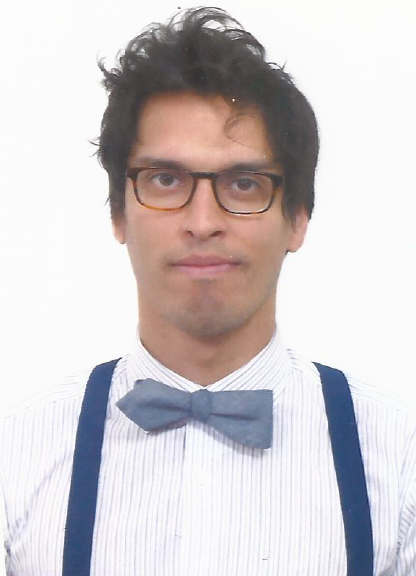
\includegraphics[width=0.2\textwidth]{1-introduction/img/georges-louis-joseph-labreche.jpg}  & \textbf{Georges L. J. Labrèche - Management Division}

\smallskip
\textit{Education}: BSc in Software Engineering with experience in technical leadership and project management in software development.

\smallskip
\textit{Responsibilities}: Acting as Systems Engineer \DIFaddbegin \DIFadd{/ Project Manager }\DIFaddend and managing overall implementation of the project \DIFaddbegin \DIFadd{until the Critical Design Review (CDR)}\DIFaddend . Establishing and overseeing product development cycle. Coordinating between different teams, project stakeholders, and documentation efforts.                          
\bigskip
\\

\DIFaddbegin 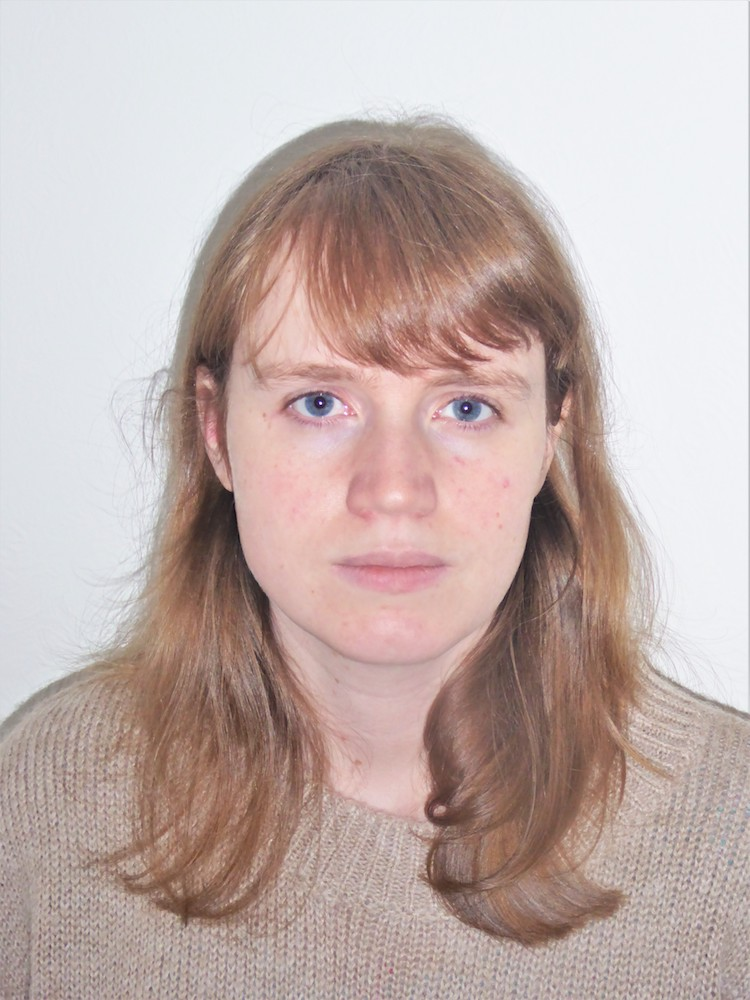
\includegraphics[width=0.2\textwidth]{1-introduction/img/natalie-lawton.jpg} & \textbf{\DIFadd{Natalie Lawton - Management and Electrical Division}}

\smallskip
\textit{\DIFadd{Education}}\DIFadd{: MEng in Aerospace Engineering. Previous experience in UAV avionic systems and emissions measurement techniques.
}

\smallskip
\textit{\DIFadd{Responsibilities}}\DIFadd{: Acting as Deputy Systems Engineer / Project Manager until the CDR. Assuming role of System Engineer / Project Manager after the CDR until end of project. Supporting designing and implementing cost-effective circuitry using analysis and computer-aided design; Reviewing and testing proposed designs; recommending modifications following prototype test results; assembling designed circuitry. 
}\bigskip
\\

\DIFaddend 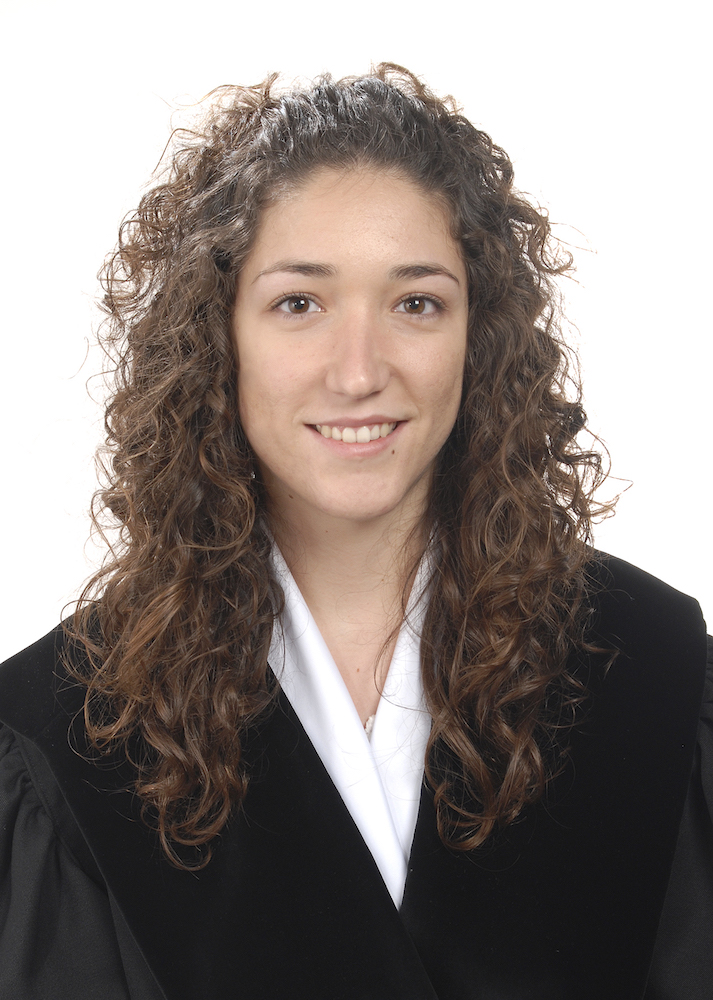
\includegraphics[width=0.2\textwidth]{1-introduction/img/agues-paszkowsky.jpg} & \textbf{Nuria Agües Paszkowsky - Scientific Division}

\smallskip
\textit{Education}: BSc in Aerospace Engineering.

\smallskip
\textit{Responsibilities}: Defining experiment parameters; data analysis; interpreting and documenting measurements; research on previous \DIFdelbegin \DIFdel{AirCore }\DIFdelend \DIFaddbegin \DIFadd{CAC }\DIFaddend experiments for comparative analysis purposes; contacting researchers or institutions working on similar projects; exploring potential partnership with researchers and institutions, evaluating the reliability of the proposed AAC sampling system; conducting measurements of collected samples; documenting and publishing findings. 
\bigskip
\\

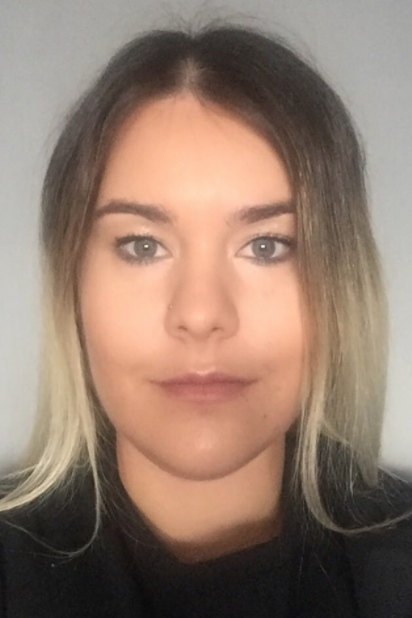
\includegraphics[width=0.2\textwidth]{1-introduction/img/kiki-blazaki.jpg} & \textbf{Kyriaki Blazaki - Scientific Division}

\smallskip
\textit{Education}: BSc in Physics.


\smallskip
\textit{Responsibilities}: Coordinating between the \DIFdelbegin \DIFdel{team }\DIFdelend \DIFaddbegin \DIFadd{Scientific Division }\DIFaddend and the Project Manager; defining experiment parameters; data analysis; interpreting and documenting measurements; research on previous \DIFdelbegin \DIFdel{AirCore }\DIFdelend \DIFaddbegin \DIFadd{CAC }\DIFaddend experiments for comparative analysis purposes; evaluating the reliability of the proposed AAC sampling system; conducting measurements of collected samples; documenting and publishing findings. 
\bigskip
\\

\DIFaddbegin 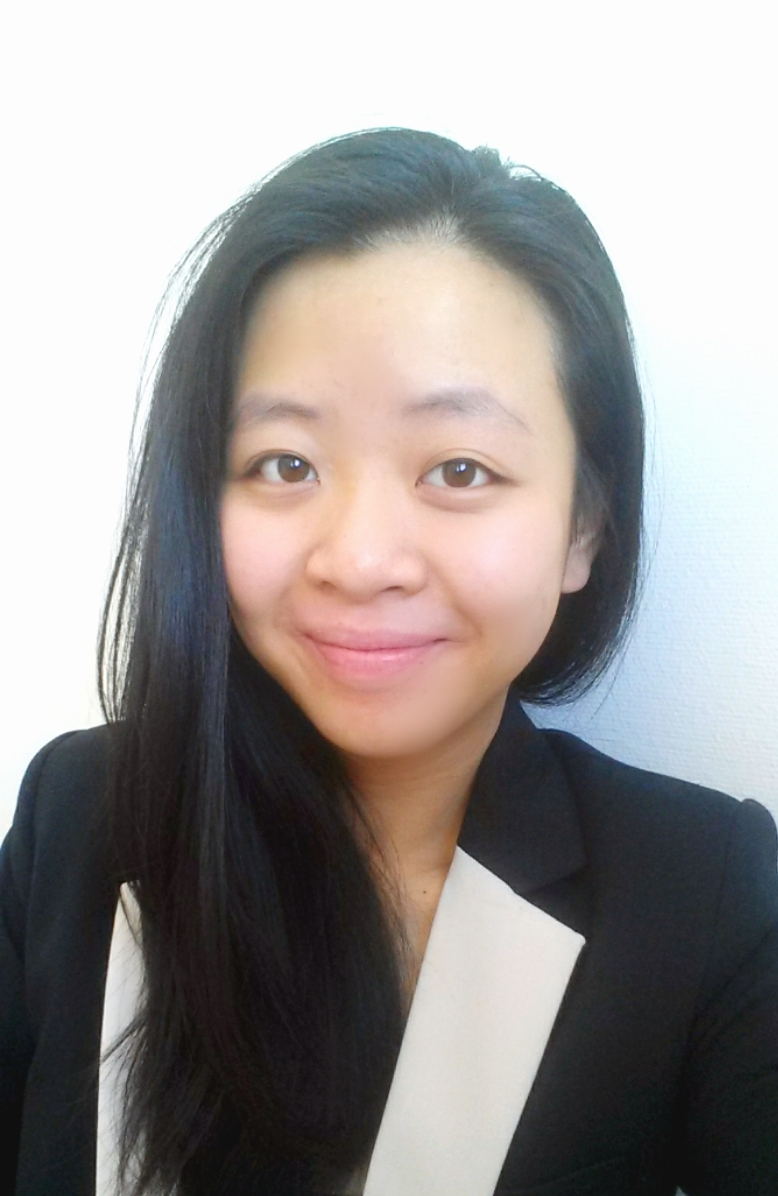
\includegraphics[width=0.2\textwidth]{1-introduction/img/emily-chen.jpeg} & \textbf{\DIFadd{Emily Chen - Mechanical Division}}

\smallskip
\textit{\DIFadd{Education}}\DIFadd{: MSc in Space Engineering (4th Year).
}


\smallskip
\textit{\DIFadd{Responsibilities}}\DIFadd{: Mechanical designing and assembly of CAC subsystem; analyzing the test results and changing the design as needed in collaboration with the team leader; integrating and assembling final design. 
}\bigskip
\\

\DIFaddend 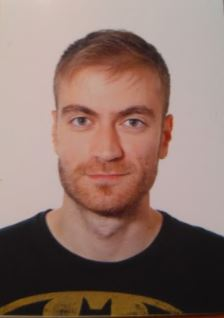
\includegraphics[width=0.2\textwidth]{1-introduction/img/jordi-coll-ortega.jpg} & \textbf{Jordi Coll Ortega - Mechanical Division}

\smallskip
\textit{Education}: BASc in Aerospace Vehicle Engineering.

\smallskip
\textit{Responsibilities}: Designing or redesigning cost-effective mechanical devices using analysis and computer-aided design; developing and testing prototypes of designed devices; analyzing the test results and changing the design as needed in collaboration with the team lead; integrating and assembling final design.
\bigskip
\\

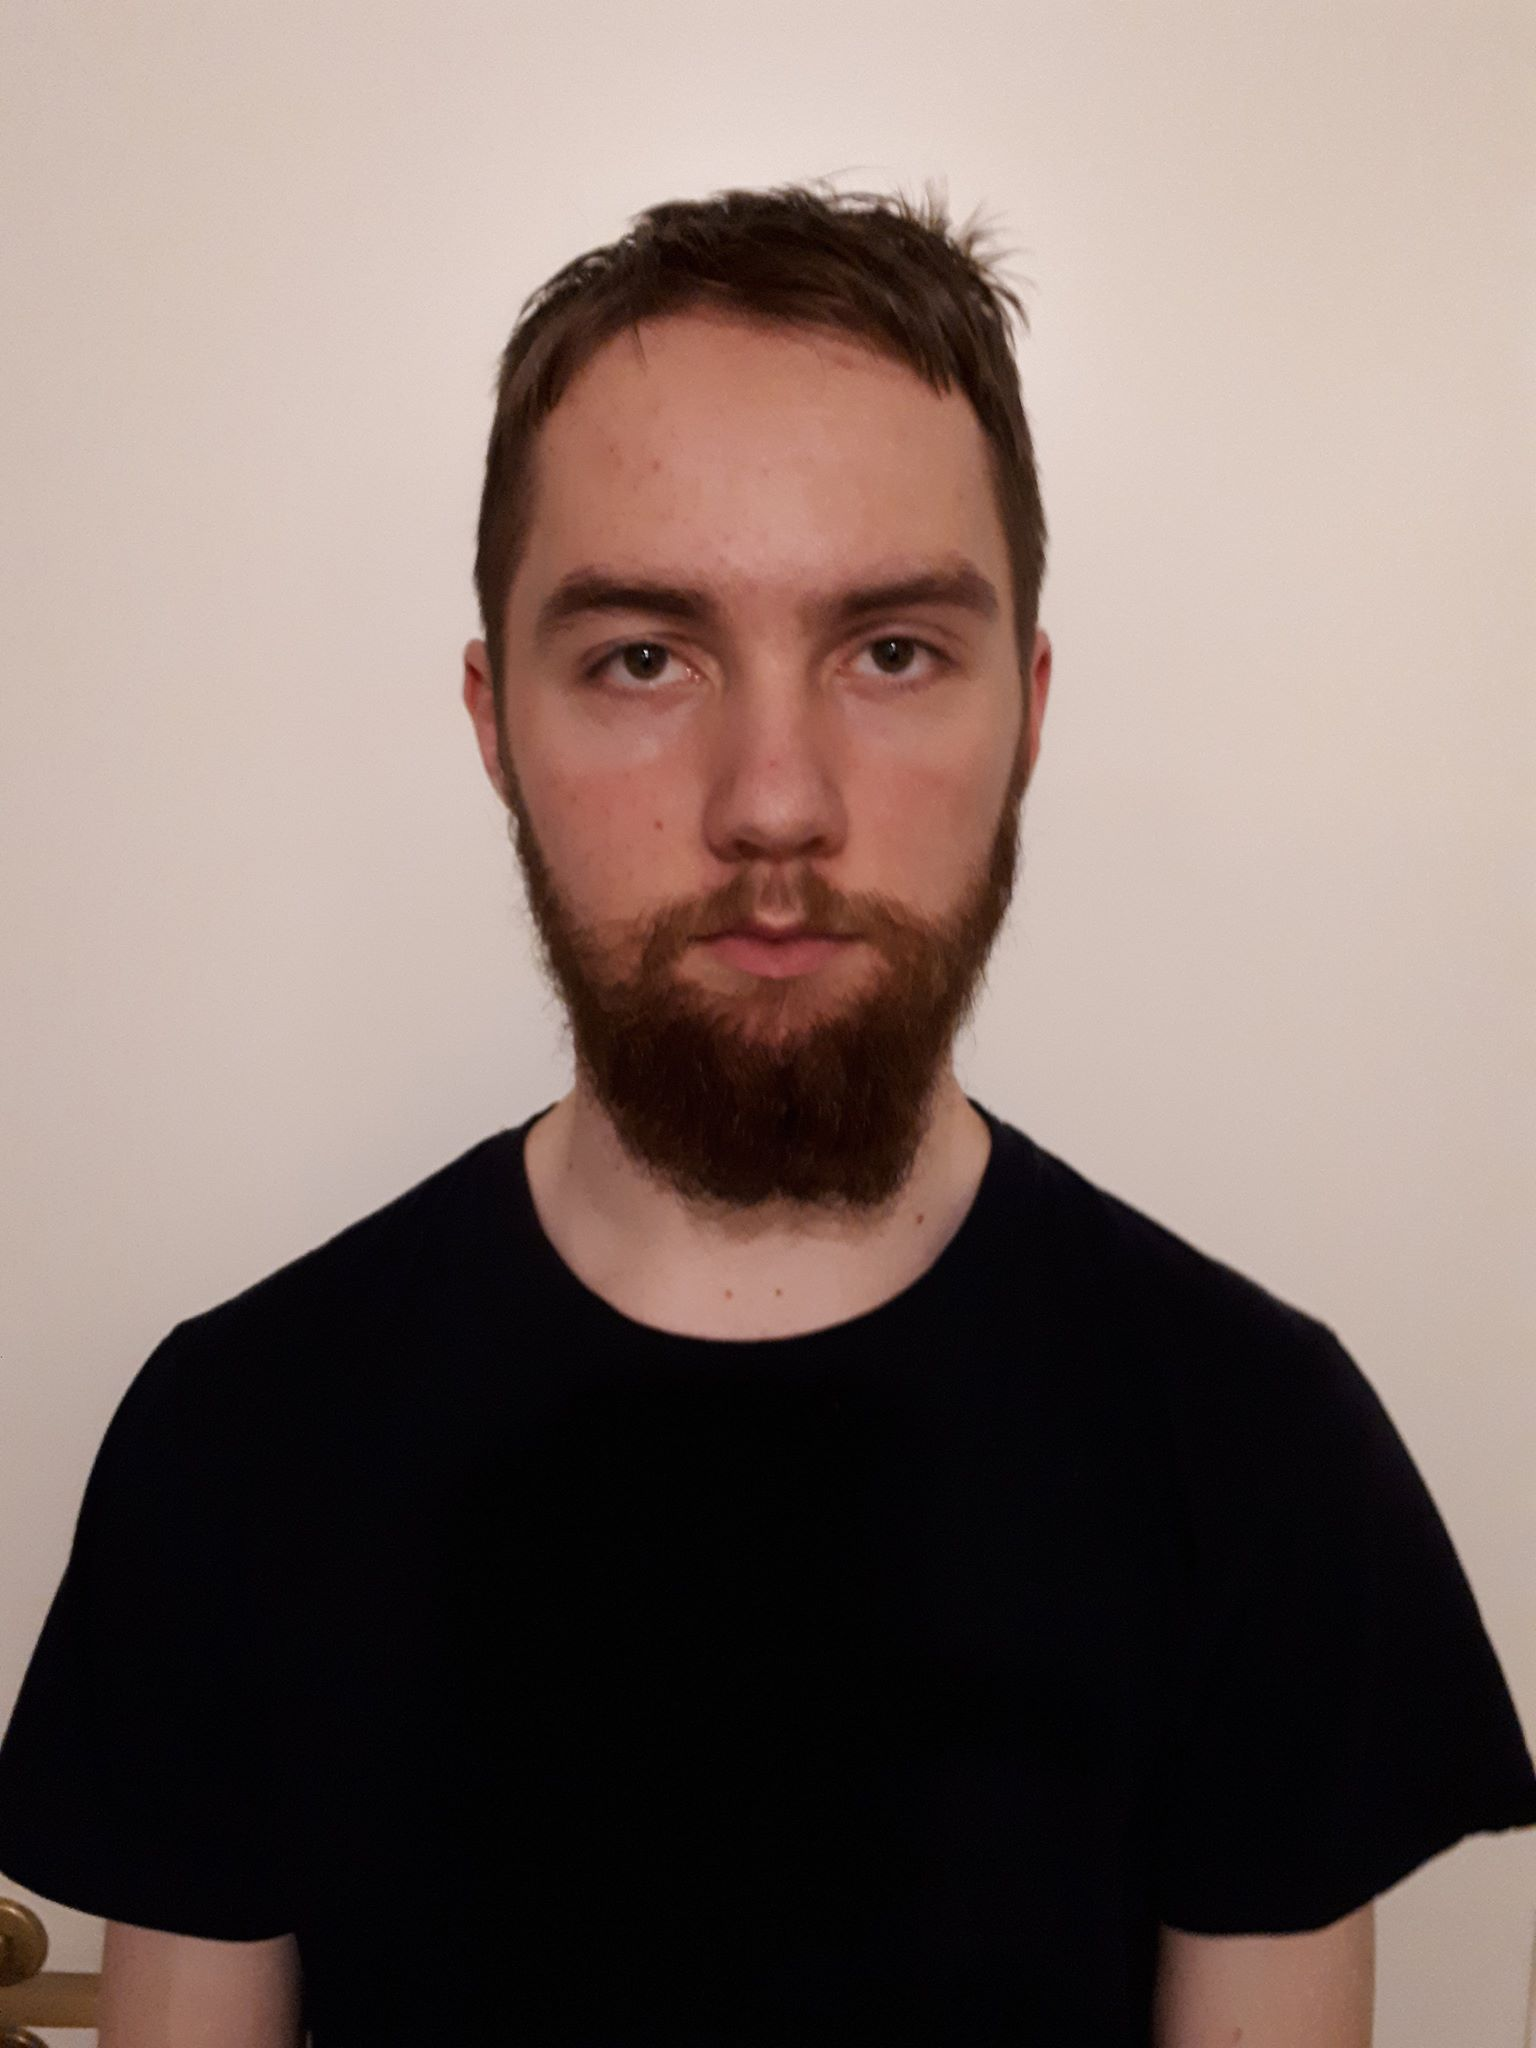
\includegraphics[width=0.2\textwidth]{1-introduction/img/gustav-dryssen.jpg} & \textbf{Gustav Dyrssen - Software Division}

\smallskip
\textit{Education}: MSc in Space Engineering (4th Year).

\smallskip
\textit{Responsibilities}: Leading quality assurance and testing efforts; Enforcing software testing best practices such as continuous integration testing and regression testing; reviewing requirements and specifications in order to foresee potential issues; provide input of functional requirements; advising on design; formalizing test cases; tracking defects and ensuring their resolution; facilitating code review sessions; supporting software implementation efforts.     
\bigskip
\\


\DIFdelbegin %DIFDELCMD < 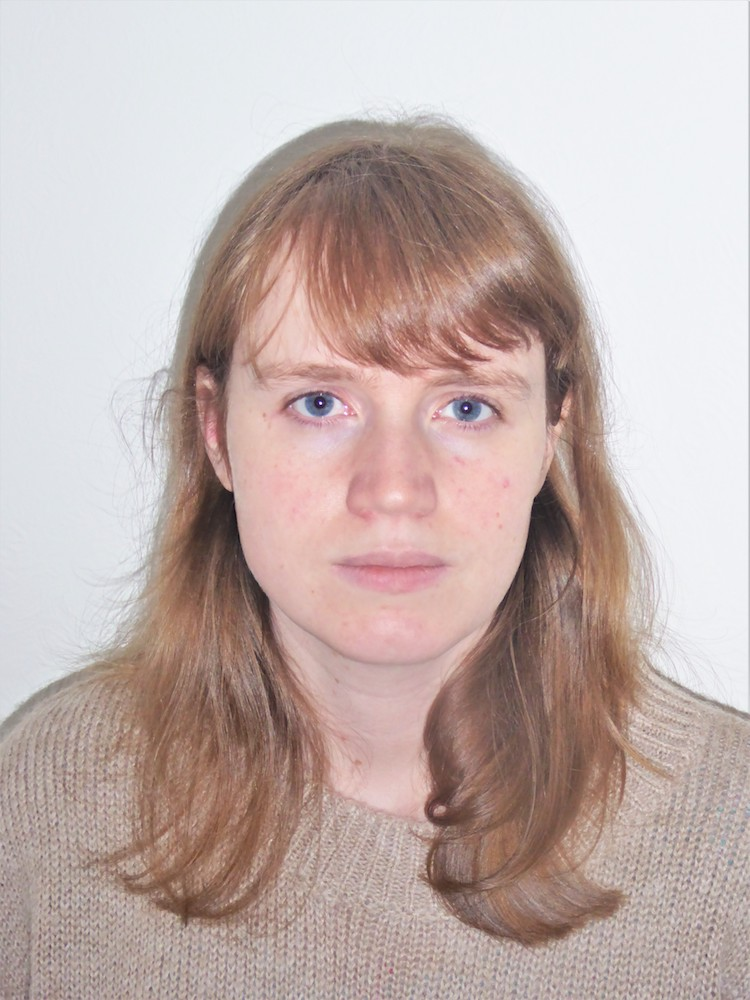
\includegraphics[width=0.2\textwidth]{1-introduction/img/natalie-lawton.jpg} %%%
\DIFdelend \DIFaddbegin 
\includegraphics[width=0.2\textwidth]{1-introduction/img/erik-fagerstrom.jpg} \DIFaddend & \textbf{\DIFdelbegin \DIFdel{Natalie Lawton }\DIFdelend \DIFaddbegin \DIFadd{Erik Fagerström }\DIFaddend - \DIFdelbegin \DIFdel{Electrical }\DIFdelend \DIFaddbegin \DIFadd{Thermal }\DIFaddend Division}

\smallskip
\textit{Education}: \DIFdelbegin \DIFdel{MEng in Aerospace Engineering . Previous experience in UAV avionic systems and emissions measurement techniques.
}\DIFdelend \DIFaddbegin \DIFadd{MSc in Space Engineering (4th Year).
}\DIFaddend 


\smallskip
\textit{Responsibilities}: \DIFdelbegin \DIFdel{Supporting designing and implementing cost-effective circuitry using analysis and computer-aided design; Reviewing and testing proposed designs; recommending modifications following prototype test results; assembling designed circuitry}\DIFdelend \DIFaddbegin \DIFadd{Coordinating between the Thermal Division and the Project Manager. Planning project thermal analysis and testing strategy. Thermal simulations of proposed designs and analyze results}\DIFaddend .
\bigskip
\\


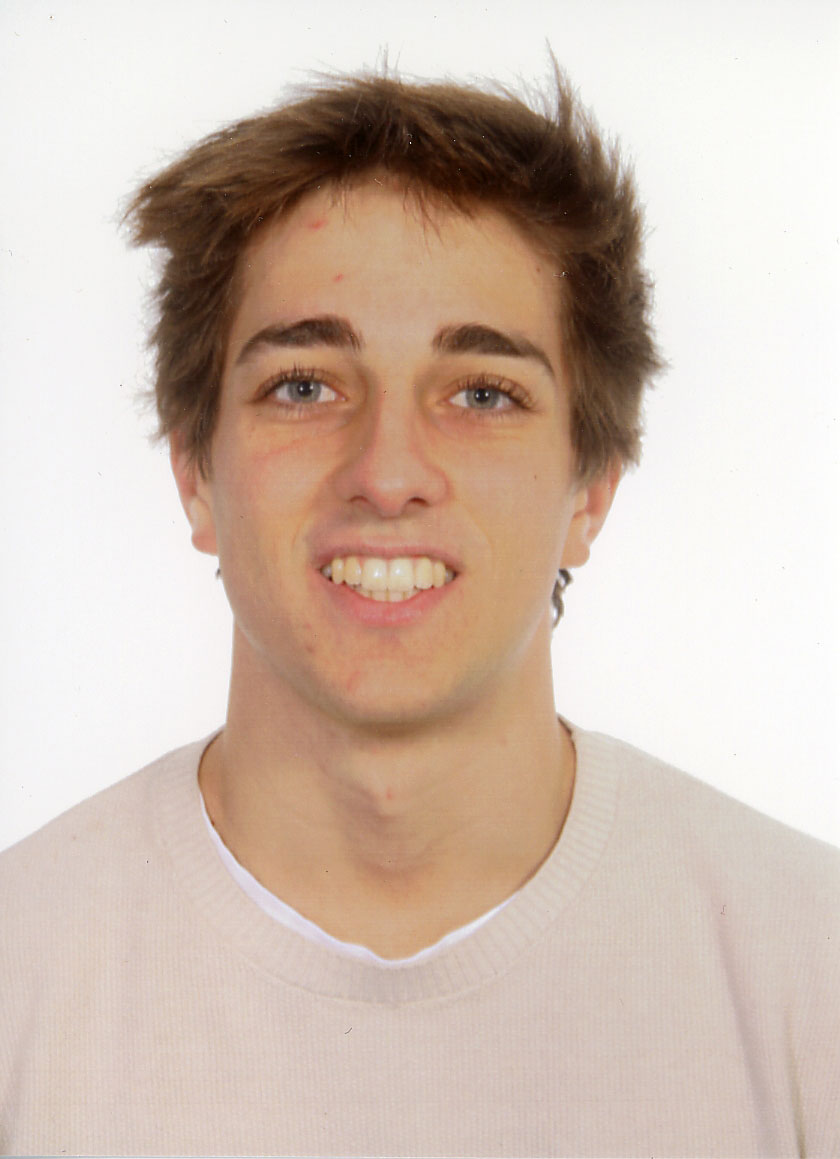
\includegraphics[width=0.2\textwidth]{1-introduction/img/pau-molas-roca.jpg} & \textbf{Pau Molas Roca - Mechanical Division}

\smallskip
\textit{Education}: BSc in Aerospace Technology Engineering, Mechanical experience.

\smallskip
\textit{Responsibilities}: Coordinating between the \DIFdelbegin \DIFdel{team }\DIFdelend \DIFaddbegin \DIFadd{Mechanical Division }\DIFaddend and the Project Manager; designing or redesigning cost-effective mechanical devices using analysis and computer-aided design; producing details of specifications and outline designs; overseeing the manufacturing process for the devices; identifying material and component suppliers; integrating and assembling final design.   \bigskip
\\


\DIFaddbegin 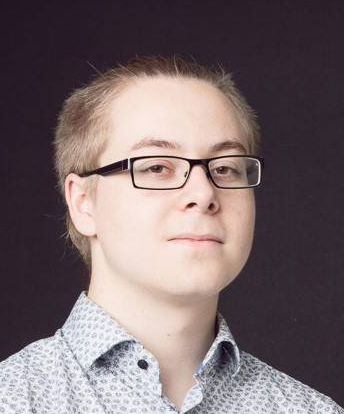
\includegraphics[width=0.2\textwidth]{1-introduction/img/emil-nordqvist.jpg} & \textbf{\DIFadd{Emil Nordqvist - Electrical Division}}

\smallskip
\textit{\DIFadd{Education}}\DIFadd{: MSc in Space Engineering (4th Year).
}

\smallskip
\textit{\DIFadd{Responsibilities}}\DIFadd{: Quality assurance of circuit design and implementation. Developing, testing, and evaluating theoretical designs.  }\bigskip
\\

\DIFaddend 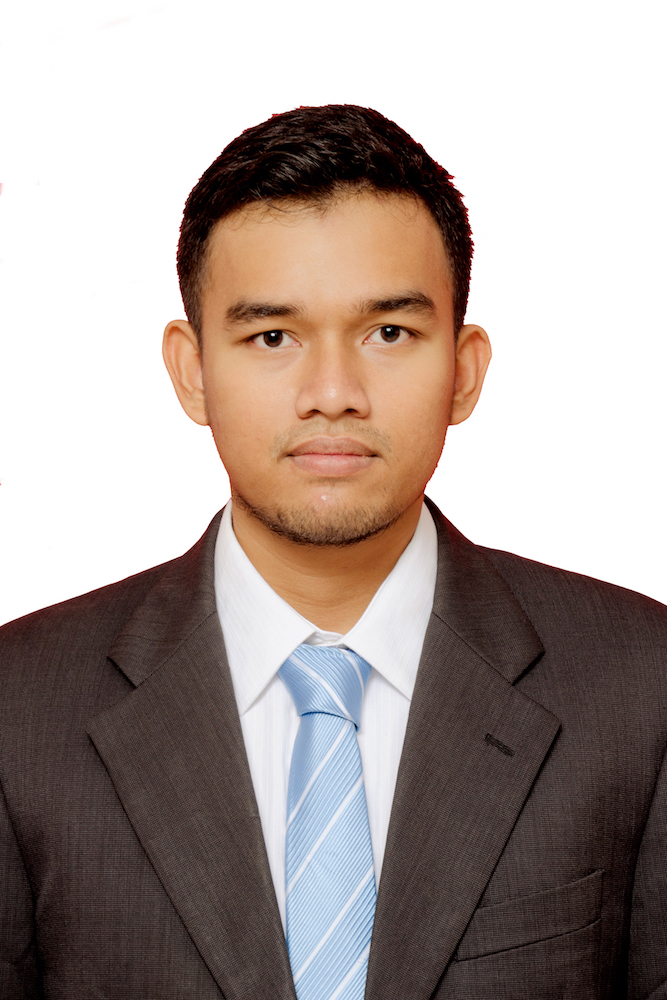
\includegraphics[width=0.2\textwidth]{1-introduction/img/muhammad-ansyar-rafi-putra.jpg} & \textbf{Muhammad Ansyar Rafi Putra - Software Division}

\smallskip
\textit{Education}: BSc in Aerospace Engineering.


\smallskip 
\textit{Responsibilities}: Coordinating between the \DIFdelbegin \DIFdel{team }\DIFdelend \DIFaddbegin \DIFadd{Software Division }\DIFaddend and the Project Manager; gathering software requirements; formalizing software specifications; drafting architecture design, detailed design; leading software implementation efforts.
\bigskip
\\

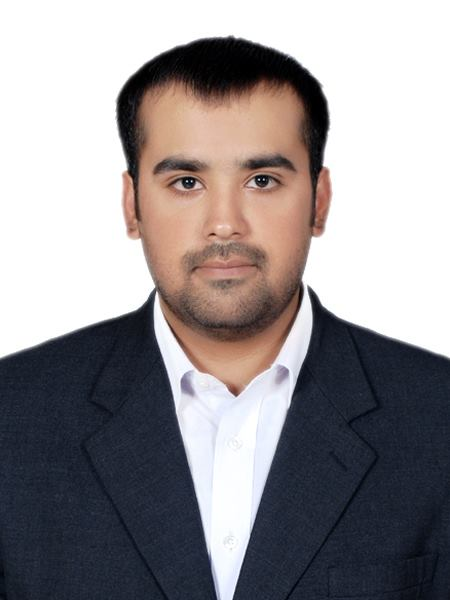
\includegraphics[width=0.2\textwidth]{1-introduction/img/hamad-saddiqi.jpg} & \textbf{Hamad Siddiqi - Electrical Division}

\smallskip
\textit{Education}: BSc in Electrical Engineering with experience in telecommunication industry and electronics.

\smallskip
\textit{Responsibilities}: Coordinating between the \DIFdelbegin \DIFdel{team }\DIFdelend \DIFaddbegin \DIFadd{Electrical Division }\DIFaddend and the Project Manager; designing and implementing cost-effective circuitry using analysis and computer-aided design; producing details of specifications and outline designs; developing, testing, and evaluating theoretical designs; identifying material as well as component suppliers. 
\bigskip
\\


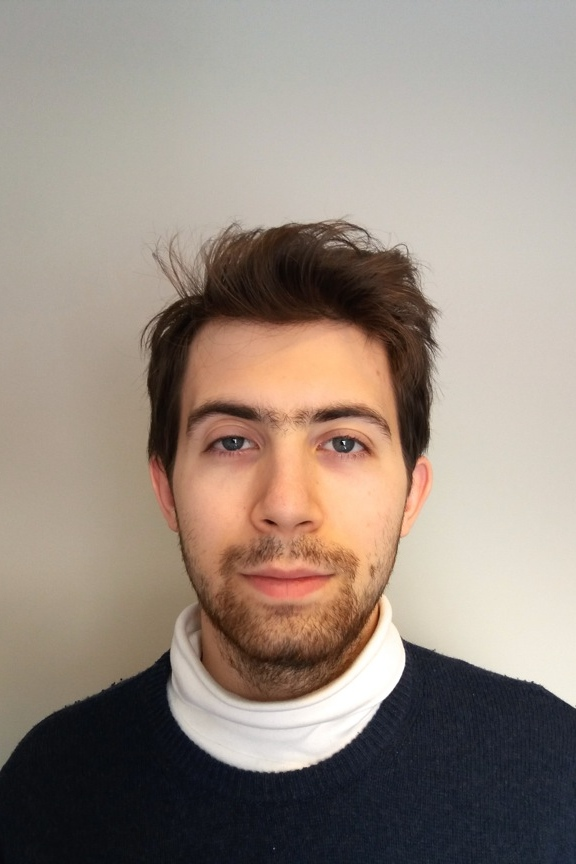
\includegraphics[width=0.2\textwidth]{1-introduction/img/ivan-zankov.jpg} & \textbf{Ivan Zankov - Thermal Division}

\smallskip
\textit{Education}: BEng in Mechanical Engineering.

\smallskip
\textit{Responsibilities}: Thermal analysis of proposed designs and \DIFdelbegin \DIFdel{Recommending modifications following thermal analysis results.                                                         
.                                                          
}\DIFdelend \DIFaddbegin \DIFadd{analysis result based recommendations.                                                         
}\DIFaddend 

\\
\label{tab:people}
\end{longtable}
\raggedbottom

\pagebreak
\section{Experiment Requirements and Constraints}
\DIFdelbegin %DIFDELCMD < 

%DIFDELCMD < %%%
\DIFdelend \subsection{Functional Requirements}

\DIFdelbegin %DIFDELCMD < \begin{enumerate}
%DIFDELCMD <     \item[F.1] %%%
\DIFdelend \DIFaddbegin \begin{enumerate}[label=F.\arabic*]
    \item \DIFaddend \st{The experiment \textit{shall} collect air samples.}\footnote{Unnecessary requirement that has been removed.\label{fn:unnecessary-requirement}}
    \DIFdelbegin %DIFDELCMD < \item[F.2] %%%
\item[\DIFdel{F.2}]%DIFAUXCMD
\DIFdelend \DIFaddbegin \item \DIFaddend The experiment \textit{shall} collect air samples by the CAC.
    \DIFdelbegin %DIFDELCMD < \item[F.3] %%%
\item[\DIFdel{F.3}]%DIFAUXCMD
\DIFdelend \DIFaddbegin \item \DIFaddend The experiment \textit{shall} collect air samples by the AAC.
    \DIFdelbegin %DIFDELCMD < \item[F.4] \st{The experiment's AAC System \textit{shall} be able to collect air samples during the ascent phase.}%%%
\item[\DIFdel{F.4}]%DIFAUXCMD
\DIFdel{\textsuperscript{\ref{fn:unnecessary-requirement}}
    }%DIFDELCMD < \item[F.5] \st{The experiment's AAC System \textit{shall} be able to collect air samples during the descent phase.}%%%
\item[\DIFdel{F.5}]%DIFAUXCMD
\DIFdel{\textsuperscript{\ref{fn:unnecessary-requirement}}
    }%DIFDELCMD < \item[F.6] %%%
\item[\DIFdel{F.6}]%DIFAUXCMD
\DIFdelend \DIFaddbegin \item \st{The experiment's AAC System \textit{shall} be able to collect air samples during the Ascent Phase.}\DIFadd{\textsuperscript{\ref{fn:unnecessary-requirement}}
    }\item \st{The experiment's AAC System \textit{shall} be able to collect air samples during the Descent Phase.}\DIFadd{\textsuperscript{\ref{fn:unnecessary-requirement}}
    }\item \DIFaddend The altitude from which a sampling bag will start sampling \textit{shall} be programmable.
    \DIFdelbegin %DIFDELCMD < \item[F.7] %%%
\item[\DIFdel{F.7}]%DIFAUXCMD
\DIFdelend \DIFaddbegin \item \DIFaddend The altitude from which a sampling bag will stop sampling \textit{shall} be programmable.
    \DIFdelbegin %DIFDELCMD < \item[F.8] %%%
\item[\DIFdel{F.8}]%DIFAUXCMD
\DIFdelend \DIFaddbegin \item \DIFaddend \st{The experiment \textit{shall} pump air into the AAC Sampling Bags.}\textsuperscript{\ref{fn:unnecessary-requirement}}
    \DIFdelbegin %DIFDELCMD < \item[F.9] %%%
\item[\DIFdel{F.9}]%DIFAUXCMD
\DIFdelend \DIFaddbegin \item \DIFaddend The experiment \textit{should} collect data on the air intake flow to the AAC.
    \DIFdelbegin %DIFDELCMD < \item[F.10] %%%
\item[\DIFdel{F.10}]%DIFAUXCMD
\DIFdelend \DIFaddbegin \item \DIFaddend The experiment \textit{shall} collect data on the air pressure.
    \DIFdelbegin %DIFDELCMD < \item[F.11] %%%
\item[\DIFdel{F.11}]%DIFAUXCMD
\DIFdelend \DIFaddbegin \item \DIFaddend The experiment \textit{shall} collect data on the temperature.
    \DIFdelbegin %DIFDELCMD < \item[F.12] %%%
\item[\DIFdel{F.12}]%DIFAUXCMD
\DIFdelend \DIFaddbegin \item \DIFaddend The experiment \textit{shall} collect data on the humidity.
    \DIFdelbegin %DIFDELCMD < \item[F.13] %%%
\item[\DIFdel{F.13}]%DIFAUXCMD
\DIFdelend \DIFaddbegin \item \DIFaddend \st{The experiment \textit{shall} measure the temperature inside the AAC Valve Box.}\textsuperscript{\ref{fn:unnecessary-requirement}}
    \DIFdelbegin %DIFDELCMD < \item[F.14] %%%
\item[\DIFdel{F.14}]%DIFAUXCMD
\DIFdelend \DIFaddbegin \item \DIFaddend \st{The experiment \textit{should} measure the humidity inside the AAC Valve Box.}\textsuperscript{\ref{fn:unnecessary-requirement}}
    \DIFdelbegin %DIFDELCMD < \item[F.15] %%%
\item[\DIFdel{F.15}]%DIFAUXCMD
\DIFdelend \DIFaddbegin \item \DIFaddend \st{The experiment \textit{shall} collect data on the time.}\footnote{Unverifiable requirement that has been removed.\label{fn:unverifiable-requirement}}
    \DIFdelbegin %DIFDELCMD < \item[F.16] %%%
\item[\DIFdel{F.16}]%DIFAUXCMD
\DIFdelend \DIFaddbegin \item \DIFaddend \st{The experiment \textit{shall} accept telecommand instructions to program AAC sampling altitudes for each sampling bag.}\textsuperscript{\ref{fn:unnecessary-requirement}}
    \DIFdelbegin %DIFDELCMD < \item[F.17] %%%
\item[\DIFdel{F.17}]%DIFAUXCMD
\DIFdelend \DIFaddbegin \item \DIFaddend \st{The experiment \textit{shall} accept telecommand instructions to open designated valves.}\textsuperscript{\ref{fn:unnecessary-requirement}}
    \DIFdelbegin %DIFDELCMD < \item[F.18] %%%
\item[\DIFdel{F.18}]%DIFAUXCMD
\DIFdelend \DIFaddbegin \item \DIFaddend \st{The experiment \textit{shall} accept telecommand instructions to close designated valves.}\textsuperscript{\ref{fn:unnecessary-requirement}}
    \DIFdelbegin %DIFDELCMD < \item[F.19] %%%
\item[\DIFdel{F.19}]%DIFAUXCMD
\DIFdelend \DIFaddbegin \item \DIFaddend \st{The experiment \textit{may} accept telecommand instructions to change the sampling rate of the ambient pressure sensor.}\textsuperscript{\ref{fn:unnecessary-requirement}}
    \DIFdelbegin %DIFDELCMD < \item[F.20] %%%
\item[\DIFdel{F.20}]%DIFAUXCMD
\DIFdelend \DIFaddbegin \item \DIFaddend \st{The experiment \textit{may} accept telecommand instructions to change the sampling rate of the ambient temperature sensor.}\textsuperscript{\ref{fn:unnecessary-requirement}}
    \DIFdelbegin %DIFDELCMD < \item[F.21] %%%
\item[\DIFdel{F.21}]%DIFAUXCMD
\DIFdelend \DIFaddbegin \item \DIFaddend \st{The experiment \textit{may} accept telecommand instructions to change the sampling rate of the AAC Valve Box temperature sensor.}\textsuperscript{\ref{fn:unnecessary-requirement}}
    \DIFdelbegin %DIFDELCMD < \item[F.22] %%%
\item[\DIFdel{F.22}]%DIFAUXCMD
\DIFdelend \DIFaddbegin \item \DIFaddend \st{The experiment \textit{may} accept telecommand instructions to turn on the air pump.}\textsuperscript{\ref{fn:unnecessary-requirement}}
    \DIFdelbegin %DIFDELCMD < \item[F.23] %%%
\item[\DIFdel{F.23}]%DIFAUXCMD
\DIFdelend \DIFaddbegin \item \DIFaddend \st{The experiment \textit{may} accept telecommand instructions to turn off the air pump.}\textsuperscript{\ref{fn:unnecessary-requirement}}
    \DIFdelbegin %DIFDELCMD < \item[F.24] %%%
\item[\DIFdel{F.24}]%DIFAUXCMD
\DIFdelend \DIFaddbegin \item \DIFaddend \st{The experiment \textit{may} accept telecommand instructions to turn on the Valve Heater.}\textsuperscript{\ref{fn:unnecessary-requirement}}
    \DIFdelbegin %DIFDELCMD < \item[F.25] %%%
\item[\DIFdel{F.25}]%DIFAUXCMD
\DIFdelend \DIFaddbegin \item \DIFaddend \st{The experiment \textit{may} accept telecommand instructions to turn off the Valve Heater.}\textsuperscript{\ref{fn:unnecessary-requirement}}
    \DIFdelbegin %DIFDELCMD < \item[F.26] %%%
\item[\DIFdel{F.26}]%DIFAUXCMD
\DIFdelend \DIFaddbegin \item \DIFaddend \st{The experiment \textit{may} accept telecommand instructions to turn on the Electronics Box Heater.}\textsuperscript{\ref{fn:unnecessary-requirement}}
    \DIFdelbegin %DIFDELCMD < \item[F.27] %%%
\item[\DIFdel{F.27}]%DIFAUXCMD
\DIFdelend \DIFaddbegin \item \DIFaddend \st{The experiment \textit{may} accept telecommand instructions to turn off the Electronics Box Heater.}\textsuperscript{\ref{fn:unnecessary-requirement}}
\end{enumerate}
\pagebreak
\subsection{Performance Requirements}

\begin{enumerate}[label=P.\arabic*]
    \item \DIFdelbegin %DIFDELCMD < \st{The telecommand data rate \textit{shall} be 10Kb/s.}%%%
\DIFdelend \DIFaddbegin \st{The telecommand data rate \textit{shall} be 10 Kb/s.}\DIFaddend \footnote{Moved to design requirements.\DIFdelbegin %DIFDELCMD < \label{fn:design-requirement}%%%
\DIFdelend \DIFaddbegin \label{designRequirement}\DIFaddend }
    \item \st{The default sampling rate of the ambient pressure sensor during Standby mode \textit{shall} be 0.1 Hz.}\footnote{Replaced by \ref{newsamplerate}\label{replaceSampleRate}}
    \item \st{The default sampling rate of the ambient pressure sensor during Normal operation-ascent mode \textit{shall} be 0.2 Hz.}\textsuperscript{\ref{replaceSampleRate}}
    \item \st{The default sampling rate of the ambient pressure sensor during Normal operation-descent mode \textit{shall} be 10 Hz.}\textsuperscript{\ref{replaceSampleRate}}
    %\item The default sampling rate of the ambient pressure sensor \textit{shall} be TBD.
    \item \st{The default sampling rate of the AAC Valve Box temperature sensor \textit{shall} be 1 Hz.}\textsuperscript{\ref{replaceSampleRate}}
    \item \st{The programmable sampling rate of the ambient pressure sensor \textit{shall} not be lesser than 0.1 Hz.}\textsuperscript{\ref{replaceSampleRate}}
    \item \st{The programmable sampling rate of the ambient pressure sensor \textit{shall} not be greater than 100 Hz.}\textsuperscript{\ref{replaceSampleRate}}
    \item \DIFdelbegin %DIFDELCMD < \st{The programmable sampling rate of the Electronics Box temperature sensor \textit{shall} not be lesser than 1Hz.}%%%
\DIFdelend \DIFaddbegin \st{The programmable sampling rate of the Electronics Box temperature sensor \textit{shall} not be lesser than 1 Hz.}\DIFaddend \textsuperscript{\ref{replaceSampleRate}}
    \item \DIFdelbegin %DIFDELCMD < \st{The programmable sampling rate of the Electronics Box temperature sensor \textit{shall} not be greater than 7Hz.}%%%
\DIFdelend \DIFaddbegin \st{The programmable sampling rate of the Electronics Box temperature sensor \textit{shall} not be greater than 7 Hz.}\DIFaddend \textsuperscript{\ref{replaceSampleRate}}
    \item \st{The programmable sampling rate of the AAC Valve Box temperature sensor \textit{shall} not be lesser than 1 Hz.}\textsuperscript{\ref{replaceSampleRate}}
    \item \st{The programmable sampling rate of the AAC Valve Box temperature sensor \textit{shall} not be greater than 7 Hz.}\textsuperscript{\ref{replaceSampleRate}}
    %\item The programmable sampling rate of the pressure sensor \textit{shall} not be lesser than .
    \item The accuracy of the ambient pressure measurements \textit{shall} be -1.5/+1.5 mbar for 25$\degree$C.
    \item The accuracy of temperature measurements \textit{shall} be +3.5/\DIFdelbegin \DIFdel{-2}\DIFdelend \DIFaddbegin \DIFadd{-3}\DIFaddend $\degree$C (max) for condition of -55$\degree$C to 150$\degree$C.
    \item The accuracy of the ambient humidity measurements \textit{shall} be ±3\%. \cite{Humiditysensor}
    \item \DIFdelbegin %DIFDELCMD < \st{The accuracy of the AAC Valve Box temperature measurements \textit{shall} be +3.5/-2°C(max).}%%%
\DIFdelend \DIFaddbegin \st{The accuracy of the AAC Valve Box temperature measurements \textit{shall} be +3.5/-2\mbox{%DIFAUXCMD
$\degree$
}%DIFAUXCMD
C(max).}\DIFaddend \footnote{Combined with P13\label{fn:combi-p13}}
    \item \DIFdelbegin \DIFdel{The air intake rate of the air pump }\textit{\DIFdel{shall}} %DIFAUXCMD
\DIFdel{be minimum 3L/min.
    }\DIFdelend \DIFaddbegin \st{The air intake rate of the air pump \textit{shall} be minimum 3 L/min.}\DIFadd{\textsuperscript{\ref{designRequirement}}
    }\DIFaddend \item \DIFdelbegin \DIFdel{The temperature of the Electronics Box }\textit{\DIFdel{shall}} %DIFAUXCMD
\DIFdel{be between 0\mbox{%DIFAUXCMD
$\degree$
}%DIFAUXCMD
C and 25\mbox{%DIFAUXCMD
$\degree$
}%DIFAUXCMD
C.
    }\DIFdelend \DIFaddbegin \st{The temperature of the Electronics Box \textit{shall} be between 0\mbox{%DIFAUXCMD
$\degree$
}%DIFAUXCMD
C and 25\mbox{%DIFAUXCMD
$\degree$
}%DIFAUXCMD
C.} \DIFadd{\textsuperscript{\ref{designRequirement}}
    }\DIFaddend \item \st{The temperature of the Electronics Box \textit{shall} not exceed 25$\degree$C.}\footnote{Combined with P17 \DIFaddbegin \DIFadd{and moved to design requirements.}\DIFaddend \label{fn:combi-p17}}
    \item \DIFdelbegin \DIFdel{The temperature of the AAC Valve Box }\textit{\DIFdel{shall}} %DIFAUXCMD
\DIFdel{be between 0\mbox{%DIFAUXCMD
$\degree$
}%DIFAUXCMD
C and 25\mbox{%DIFAUXCMD
$\degree$
}%DIFAUXCMD
C.
    }\DIFdelend \DIFaddbegin \st{The temperature of the AAC Valve Box \textit{shall} be between 0\mbox{%DIFAUXCMD
$\degree$
}%DIFAUXCMD
C and 25\mbox{%DIFAUXCMD
$\degree$
}%DIFAUXCMD
C.}\DIFadd{\textsuperscript{\ref{designRequirement}}
    }\DIFaddend \item \st{The temperature of the AAC Valve Box \textit{shall} not exceed 25$\degree$C.}\footnote{Combined with P19 \DIFaddbegin \DIFadd{and moved to design requirements.}\DIFaddend \label{fn:combi-p19}}
    \item \DIFdelbegin \DIFdel{The air sampling systems }\textit{\DIFdel{shall}} %DIFAUXCMD
\DIFdel{filter out all water molecules before filling the sampling containers.
    }\DIFdelend \DIFaddbegin \st{The air sampling systems \textit{shall} filter out all water molecules before filling the sampling containers.} \DIFadd{\textsuperscript{\ref{designRequirement}}
    }\DIFaddend \item \st{The CAC air sampling \textit{shall} filter out all water molecules before filling the tube.}\footnote{Combined with P21 \DIFaddbegin \DIFadd{and moved to design requirements.}\DIFaddend \label{fn:combi-p21}}
    \item The sensors sampling rate \textit{shall} be \DIFdelbegin \DIFdel{2Hz}\DIFdelend \DIFaddbegin \DIFadd{2 Hz}\DIFaddend .\label{newsamplerate}
    \item The temperature of the Pump \DIFdelbegin \DIFdel{Box }\DIFdelend \textit{shall} be between 5$\degree$C and \DIFdelbegin \DIFdel{25}\DIFdelend \DIFaddbegin \DIFadd{40}\DIFaddend $\degree$C. 
    \DIFaddbegin \item \DIFadd{The minimum volume of air in the bags for analysis }\textit{\DIFadd{shall}} \DIFadd{be 0.18 L at ground level.
 }\DIFaddend \end{enumerate} 
\pagebreak
\subsection{Design Requirements}

\begin{enumerate}[label=D.\arabic*]
    \item The experiment \textit{shall} operate in the temperature profile of the BEXUS flight.
    \item The experiment \textit{shall} operate in the vibration profile of the BEXUS flight.
    \item \st{The experiment \textit{shall} not disturb or harm the launch vehicle.}\textsuperscript{\ref{fn:unnecessary-requirement}}
    \item The experiment's communication system \textit{shall} be compatible with the gondola's E-link system.
    \item The experiment's power supply \textit{shall} be compatible with the gondola's provided power.
    \item \st{The experiment \textit{shall} not disturb other experiments on the gondola.}\textsuperscript{\ref{fn:unnecessary-requirement}}
    \item The total DC current draw \textit{should} be below 1.8 A.
    \item The total power consumption \textit{should} be below 374 Wh.
    \item \DIFdelbegin \DIFdel{The experiment }\textit{\DIFdel{shall}} %DIFAUXCMD
\DIFdel{be able to operate in low pressure conditions (10-15 mbar) up to 30 km altitude.
    }\DIFdelend \DIFaddbegin \st{The experiment \textit{shall} be able to operate in low pressure conditions (10-15 mbar) up to 30 km altitude.}\footnote{\DIFadd{Repeated in D18}\label{fn:repeat-d18}}
    \DIFaddend \item \st{The components of the experiment \textit{shall} operate within their temperature ranges.}\textsuperscript{\ref{fn:unnecessary-requirement}}
    \item \st{The OBC \textit{shall} be able to autonomously control the heaters.}\textsuperscript{\ref{fn:unnecessary-requirement}}
    \item \st{The ground station GC \textit{shall} be able to display some of the received data.}\textsuperscript{\ref{fn:unnecessary-requirement}}
    \item \st{The experiment \textit{shall} be able to survive and operate between -30\degree C and 60\degree C.}\textsuperscript{\ref{fn:unnecessary-requirement}}
    \item \st{The external components that are directly exposed to the outside environment \textit{shall} be able to operate at -70\degree C.}\textsuperscript{\ref{fn:unnecessary-requirement}}
    \item \st{The watchdog \textit{should} be able to reset the system.}\textsuperscript{\ref{fn:unnecessary-requirement}}
    \item The experiment \textit{shall} be able to autonomously turn itself off just before landing.
    \item The experiment box \textit{shall} be placed with at least one face exposed to the outside.
    \item The experiment \textit{shall} operate in the pressure profile of the BEXUS flight.
    \item The experiment \textit{shall} operate in the vertical \DIFdelbegin \DIFdel{accelerations profile of the BEXUS flight.
    }%DIFDELCMD < \item %%%
\item%DIFAUXCMD
\DIFdel{The experiment }\textit{\DIFdel{shall}} %DIFAUXCMD
\DIFdel{operate in the
    }\DIFdelend \DIFaddbegin \DIFadd{and }\DIFaddend horizontal accelerations profile of the BEXUS flight.
    \item \DIFaddbegin \st{The experiment \textit{shall} operate in the
    horizontal accelerations profile of the BEXUS flight.}\footnote{\DIFadd{Combined with D19}\label{fn:combi-d19}}
    \item \DIFaddend The experiment \textit{shall} be attached to the gondola's rails.
    \item The telecommand data rate \textit{shall} not be over \DIFdelbegin \DIFdel{10kb}\DIFdelend \DIFaddbegin \DIFadd{10 kb}\DIFaddend /s.
    \DIFaddbegin \item \DIFadd{The air intake rate of the air pump }\textit{\DIFadd{shall}} \DIFadd{be minimum 3 L/min at 24 km altitude.
    }\item \DIFadd{The temperature of the Brain }\textit{\DIFadd{shall}} \DIFadd{be between -10\mbox{%DIFAUXCMD
$\degree$
}%DIFAUXCMD
C and 25\mbox{%DIFAUXCMD
$\degree$
}%DIFAUXCMD
C.
    }\item \st{The temperature of the Brain level 2 \textit{shall} be between 0\mbox{%DIFAUXCMD
$\degree$
}%DIFAUXCMD
C and 25\mbox{%DIFAUXCMD
$\degree$
}%DIFAUXCMD
C.} \footnote{\DIFadd{Combined with D24}\label{fn:combi-d24}}
    \item \DIFadd{The air sampling systems }\textit{\DIFadd{shall}} \DIFadd{filter out all water molecules before filling the sampling bags.
    }\item \DIFadd{The total weight of the experiment }\textit{\DIFadd{shall}} \DIFadd{be less than 28 kg.
    }\item \DIFadd{The AAC box }\textit{\DIFadd{shall}} \DIFadd{be able to fit at least \mbox{%DIFAUXCMD
$6$
}%DIFAUXCMD
air sampling bags.
    }\item \DIFadd{The CAC box }\textit{\DIFadd{shall}} \DIFadd{take less than 3 minutes to be removed from the gondola without removing the whole experiment.
    }\item \DIFadd{The AAC }\textit{\DIFadd{shall}} \DIFadd{be re-usable for future balloon flights.
}\DIFaddend \end{enumerate}
\pagebreak
\pagebreak
\subsection{Operational Requirements}

\begin{enumerate}[label=O.\arabic*]
    \item \st{The TUBULAR Team \textit{shall} send telecommands from the ground station to the experiment before and during the flight.}\textsuperscript{\ref{fn:unnecessary-requirement}}
    \item \st{The TUBULAR Team \textit{shall} receive telemetry from the experiment during the flight.}\textsuperscript{\ref{fn:unnecessary-requirement}}
    \item \st{The experiment \textit{shall} change modes autonomously.}\textsuperscript{\ref{fn:unnecessary-requirement}}
    \item \st{The heating mechanism \textit{shall} work autonomously.}\textsuperscript{\ref{fn:unnecessary-requirement}}
    \item \st{The experiment \textit{shall} store data autonomously.}\textsuperscript{\ref{fn:unnecessary-requirement}}
    \item \st{The Air sampling control system \textit{shall} work autonomously.}\textsuperscript{\ref{fn:unnecessary-requirement}}
    \item \st{The valves in air sampling control system \textit{should} be controllable from the ground station.}\textsuperscript{\ref{fn:unnecessary-requirement}}
    \item \st{The experiment \textit{should} be able to handle a timeout or drop in the network connection.}\textsuperscript{\ref{fn:unnecessary-requirement}}
    \item \st{The heaters \textit{should} be controllable from the ground station.}\textsuperscript{\ref{fn:unnecessary-requirement}}
    \item \st{The watchdog\footnote{Explained in subsection 4.8. Software Design} \textit{should} be able to reset the system.}\textsuperscript{\ref{fn:unnecessary-requirement}}
    \item \st{The system \textit{should} be able to be reset with a command from the ground station.}\textsuperscript{\ref{fn:unnecessary-requirement}}
    \item \st{The experiment \textit{should} enter different modes with a telecommand from the ground station.}\textsuperscript{\ref{fn:unnecessary-requirement}}
    \item The experiment \textit{should} function automatically.
    \item The experiment's air sampling mechanisms \textit{shall} have a manual override.
\end{enumerate} 
\pagebreak
\subsection{Constraints}

\begin{enumerate}[label=C.\arabic*]
    \item Constraints specified in the BEXUS User Manual.
    \item \st{The person-hours allocated to project implementation is limited by university related factors such as exams, assignments, and lectures.}\textsuperscript{\ref{fn:unnecessary-requirement}}
    \item \st{Budget limited to TBD.}\textsuperscript{\ref{fn:unnecessary-requirement}}
    \item \DIFdelbegin %DIFDELCMD < \st{The dimensions show a minimum print area of 50 x 50 cm and 65cm height experiment box.}%%%
\DIFdelend \DIFaddbegin \st{The dimensions show a minimum print area of 50 x 50 cm and 65 cm height experiment box.}\DIFaddend \textsuperscript{\ref{fn:unnecessary-requirement}}
\end{enumerate}



\pagebreak
\section{Project Planning}
\DIFaddbegin 

\DIFaddend \subsection{Work Breakdown Structure}

The team is categorized into different groups of responsibilities with dedicated leaders who will report to and coordinate with the \DIFdelbegin \DIFdel{project manager}\DIFdelend \DIFaddbegin \DIFadd{Project Manager}\DIFaddend . Leadership may be organized on a rotational basis should the need arise. The formation of these \DIFdelbegin \DIFdel{subteams }\DIFdelend \DIFaddbegin \DIFadd{divisions }\DIFaddend constitute a work breakdown \DIFdelbegin \DIFdel{team }\DIFdelend structure in which \DIFdelbegin \DIFdel{a simplified version }\DIFdelend is illustrated in Figure \ref{fig:work-breakdown-structure}\DIFdelbegin \DIFdel{:
}\DIFdelend \DIFaddbegin \DIFadd{.
}\DIFaddend 


\DIFdelbegin %DIFDELCMD < \begin{figure}[H]
%DIFDELCMD <     %%%
\begin{align*}
        \DIFdelFL{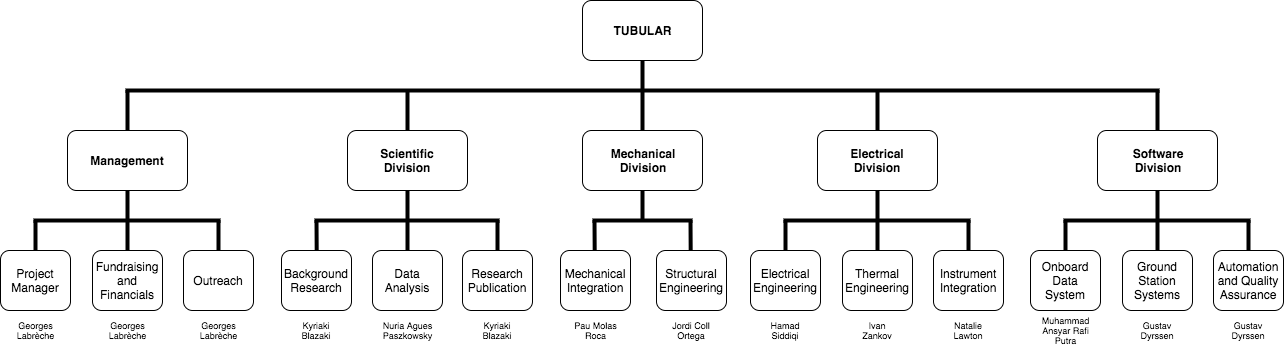
\includegraphics[width=16cm]{3-project-planning/img/work-breakdown-structure.png}
    }\end{align*}
    %DIFAUXCMD
%DIFDELCMD < \caption{%
{%DIFAUXCMD
\DIFdelFL{Work Breakdown Structure}}%DIFAUXCMD
%DIFDELCMD < \label{fig:work-breakdown-structure}
%DIFDELCMD < \end{figure}
%DIFDELCMD < 

%DIFDELCMD < %%%
\DIFdelend The interaction between the \DIFdelbegin \DIFdel{subteams }\DIFdelend \DIFaddbegin \DIFadd{divisions }\DIFaddend will be refined over the course of project implementation to acknowledge the interdisciplinary nature of the experiment around a Payload / Platform scheme.

The Management is composed of a Project Manager \DIFdelbegin \DIFdel{acting as the }\DIFdelend \DIFaddbegin \DIFadd{and a Deputy Project Manager, both acting as }\DIFaddend Systems Engineer and managing overall implementation of the project. The Project Manager is responsible for establishing and overseeing product development cycle; coordinating between different teams, project stakeholders, and documentation efforts; outreach and public relations; Fundraising; monitoring and reporting; system integration; and quality assurance. \DIFaddbegin \DIFadd{The Deputy Project Manager assists the Project Manager in all management duties in a manner that ensures replaceability when necessary.
}\DIFaddend 

The Scientific Division is responsible for defining experiment parameters; data analysis; interpreting and documenting measurements; researching previous \DIFdelbegin \DIFdel{AirCore }\DIFdelend \DIFaddbegin \DIFadd{CAC }\DIFaddend experiments for comparative analysis purposes; evaluating the reliability of the proposed AAC sampling system; conducting measurements of collected samples; documenting and publishing findings; defining experiment parameters; contacting researchers or institutions working on similar projects; exploring potential partnership with researchers and institutions; documenting and publishing findings.

The Mechanical Division is responsible for designing or redesigning cost-effective mechanical devices using analysis and computer-aided design; producing details of specifications and outline designs; overseeing the manufacturing process for the devices; identifying material and component suppliers; developing and testing prototypes of designed devices; analyzing test results and changing the design as needed; and integrating and assembling final design.

The Electrical Division is responsible for designing and implementing cost-effective circuitry using analysis and computer-aided design; producing details of specifications and outline designs; developing, testing, and evaluating theoretical designs; identifying material as well as component suppliers; reviewing and testing proposed designs; recommending modifications following prototype test results; and assembling designed circuitry.

The Software Division is responsible for gathering software requirements; formalizing software specifications; drafting architecture design; leading software implementation efforts; leading quality assurance and testing efforts; enforcing software testing best practices such as continuous integration testing and regression testing; reviewing requirements and specifications in order to foresee potential issues; providing input for functional requirements; advising on design; formalizing test cases; tracking defects and ensuring their resolution; facilitating code review sessions; and supporting software implementation efforts.
\DIFaddbegin 

\DIFadd{The Thermal Division is responsible for ensuring thermal regulation of the payload as per operational requirements of all experiment components; evaluating designs against thermal simulation and propose improvements; managing against mechanical design and electrical power limitations towards providing passive and active thermal control systems.
}

\begin{landscape}
\begin{figure}[p]
    \begin{align*}
        \DIFaddFL{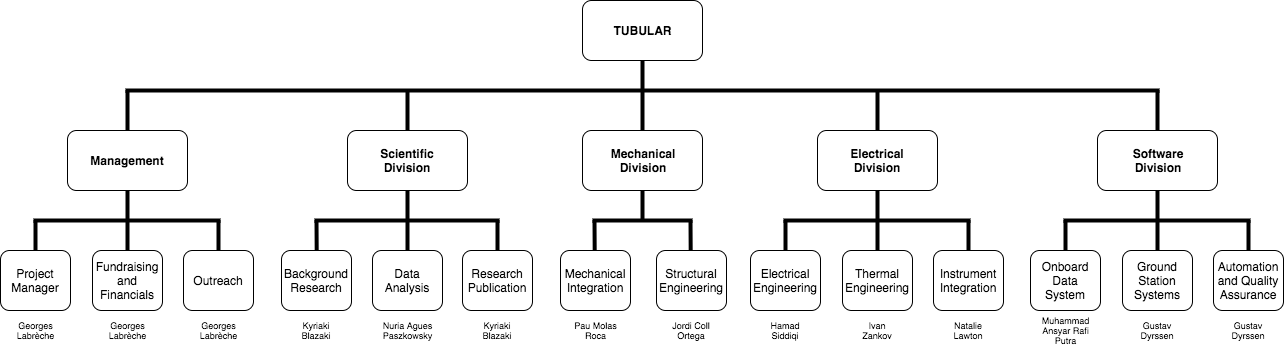
\includegraphics[width=24cm]{3-project-planning/img/work-breakdown-structure.png}
    }\end{align*}
    \caption{\DIFaddFL{Work Breakdown Structure}}\label{fig:work-breakdown-structure}
\end{figure}
\end{landscape}
\DIFaddend \pagebreak
\subsection{Schedule}

Scheduling of the project is presented in a Gantt Chart overview on Figure \ref{fig:schedule-gantt-chart}. Exam period constraints have been included in order to evaluate risks in person-day allocations to project implementation:

\begin{figure}[H]
    \begin{align*}
        \DIFdelbeginFL %DIFDELCMD < 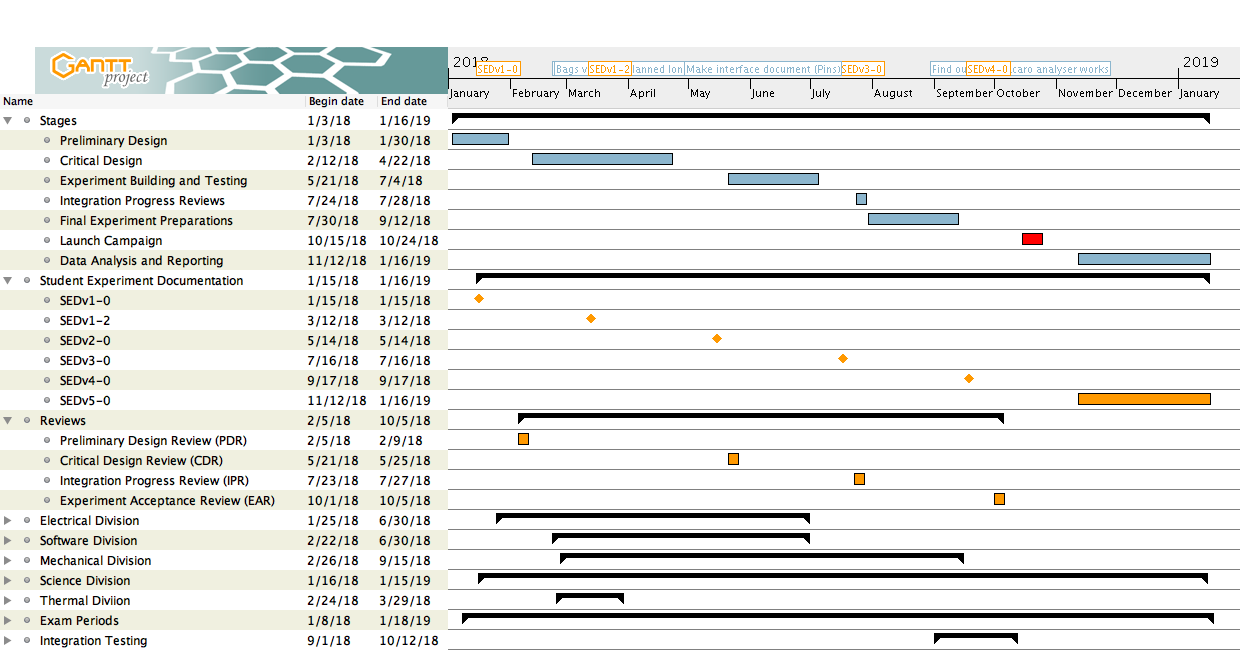
\includegraphics[width=1\linewidth]{3-project-planning/img/gantt-chart.png}
%DIFDELCMD <     %%%
\DIFdelendFL \DIFaddbeginFL 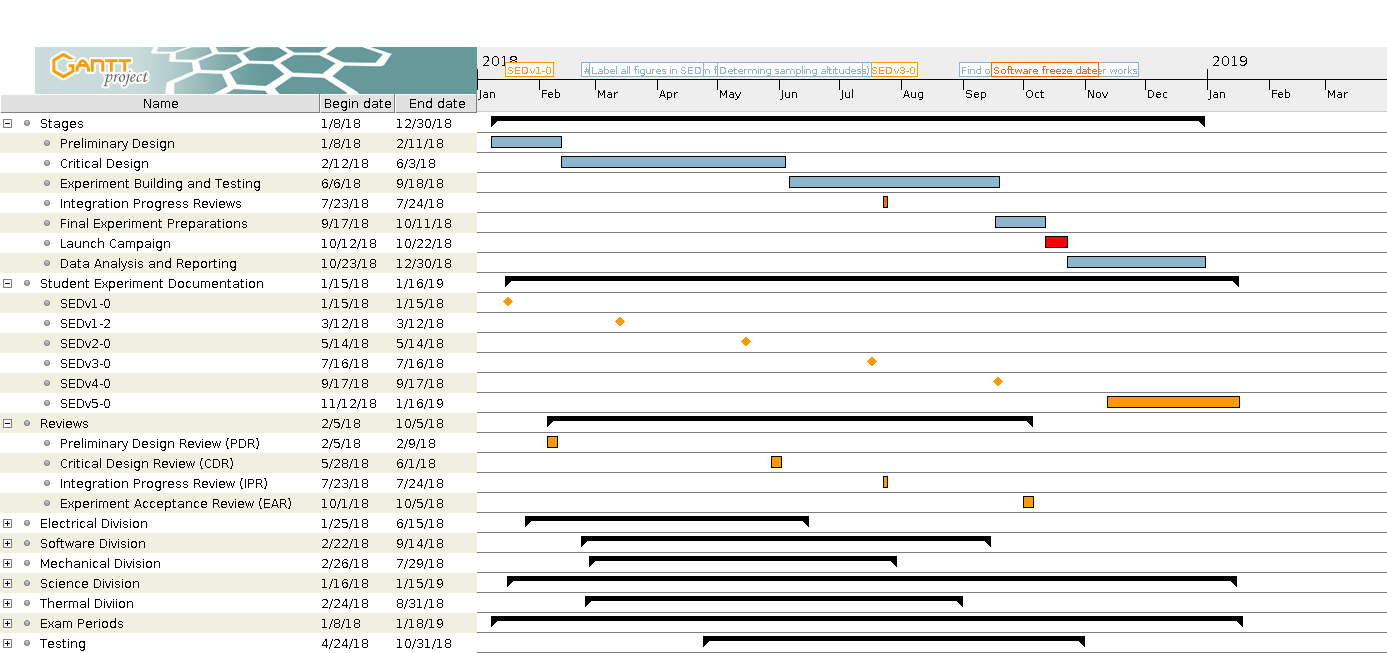
\includegraphics[width=1\linewidth]{3-project-planning/img/BEXUS-SED-GanttChart-Overview.png}
    \DIFaddendFL \end{align*}
    \caption{Project Schedule Gantt Chart}\label{fig:schedule-gantt-chart}
\end{figure}

Deadlines of the five Student Experiment Documentations (SED) versions have been estimated based on past REXUS/BEXUS Cycles. A complete Gantt Chart listing tasks for each division is shown in Appendix \ref{sec:appF}.
\pagebreak
\subsection{Resources}

\subsubsection{Manpower}
The TUBULAR \DIFdelbegin \DIFdel{team }\DIFdelend \DIFaddbegin \DIFadd{Team }\DIFaddend is categorized into divisions as summarized in Table \ref{tab:divisions-members}:

\begin{table}[H]
\centering
\DIFdelbeginFL %DIFDELCMD < \resizebox{\textwidth}{!}{%
%DIFDELCMD < \begin{tabular}{|l|l|l|l|l|l|}
%DIFDELCMD < \hline
%DIFDELCMD < \textbf{Management} & \textbf{Scientific}    & \textbf{Mechanical} & \textbf{Electrical} & \textbf{Thermal} & \textbf{Software}          \\ \hline
%DIFDELCMD < Georges Labrèche*    & Kyriaki Blazaki*        & Pau Molas Roca*      & Hamad Siddiqi*  & Ivan Zankov     & Muhammad Ansyar Rafi Putra* \\ \hline
%DIFDELCMD <                     & Nuria Agues Paszkowsky & Jordi Coll Ortega   & Natalie Lawton  &   & Gustav Dyrssen             \\ \hline
%DIFDELCMD < \end{tabular}%
%DIFDELCMD < }
%DIFDELCMD < %%%
\DIFdelendFL \DIFaddbeginFL \resizebox{\textwidth}{!}{%
\begin{tabular}{|l|l|l|l|l|l|}
\hline
\textbf{Management} & \textbf{Scientific}    & \textbf{Mechanical} & \textbf{Electrical} & \textbf{Thermal} & \textbf{Software}          \\ \hline
Georges L. J. Labrèche*    & Kyriaki Blazaki*        & Pau Molas Roca*      & Hamad Siddiqi*  & Erik Fragerström*    & Muhammad Ansyar Rafi Putra* \\ \hline
Natalie Lawton & Nuria Agues Paszkowsky & Jordi Coll Ortega   & Natalie Lawton  & Ivan Zankov  & Gustav Dyrssen             \\ \hline
 & & Emily Chen  & Emil Nordqvist  &  &              \\ \hline
\end{tabular}%
}
\DIFaddendFL \caption{Project Divisions and Members (Asterisks Denote Division Leaders)}
\label{tab:divisions-members}
\end{table}
\raggedbottom

The experience of TUBULAR \DIFdelbegin \DIFdel{team }\DIFdelend \DIFaddbegin \DIFadd{Team }\DIFaddend members are listed in Table \ref{tab:team-member-experience}:

% Please add the following required packages to your document preamble:
% \usepackage{graphicx}
\begin{table}[H]
\centering
\begin{tabular}{|l|m{11cm}|}
\hline
\textbf{Team Member} & \textbf{Project Related Experience} \\ \hline
Georges \DIFaddbeginFL \DIFaddFL{L. J. }\DIFaddendFL Labrèche & BSc in Software Engineering with experience in technical leadership and project management in software development.\\ \hline
Nuria Agues Paszkowsky & BSc in Aerospace Engineering.\\ \hline
Kyriaki Blazaki & BSc in Physics. \\ \hline
\DIFaddbeginFL \DIFaddFL{Emily Chen }& \DIFaddFL{MSc in Space Engineering (4th Year). }\\ \hline
\DIFaddendFL Jordi Coll Ortega &  BSc in Aerospace Vehicle Engineering. \\ \hline
Gustav Dyrssen &  MSc in Space Engineering (4th Year).\\ \hline
\DIFaddbeginFL \DIFaddFL{Erik Fagerström }& \DIFaddFL{MSc in Space Engineering (4th Year). }\\ \hline
\DIFaddendFL Natalie Lawton & MEng in Aerospace Engineering. Previous experience in UAV avionic systems and emissions measurement techniques. \\ \hline
Muhammad Ansyar Rafi Putra & BSc in Aerospace Engineering. \\ \hline
Pau Molas Roca & BSc in Aerospace Technology Engineering, Mechanical experience. \\ \hline
\DIFaddbeginFL \DIFaddFL{Emil Nordqvist }& \DIFaddFL{MSc in Space Engineering (4th Year). }\\ \hline
\DIFaddendFL Hamad Siddiqi & BSc in Electrical Engineering with experience in telecommunication industry and electronics.  \\ \hline
Ivan Zankov & BEng in Mechanical Engineering.\\ \hline
\end{tabular}
\caption{Project Related Experience of Team Members}
\label{tab:team-member-experience}
\end{table}
\raggedbottom

The initial projected effort to be contributed by each team member \DIFdelbegin \DIFdel{is of an average of }\DIFdelend \DIFaddbegin \DIFadd{was averaged at }\DIFaddend 1.5 hour per person per day corresponding to a team total of 15 hours per day. \DIFaddbegin \DIFadd{Since then, 3 new members have been included in the team thus increasing the projected daily effort to 19.5 hours per day. The period of these different effort capacities are listed in Table \ref{tab:daily-team-effort-per-period}:
}

\begin{table}[H]
\centering
\begin{tabular}{|c|c|c|}
\hline
\textbf{\DIFaddFL{From}} & \textbf{\DIFaddFL{To}} & \textbf{\DIFaddFL{Capacity (hours/day)}} \\ \hline
\DIFaddFL{08/01/2018 }& \DIFaddFL{18/03/2018 }& \DIFaddFL{15 }\\ \hline
\DIFaddFL{19/03/2018 }& \DIFaddFL{08/04/2018 }& \DIFaddFL{16.5 }\\ \hline
\DIFaddFL{09/04/2018 }& \DIFaddFL{09/05/2018 }& \DIFaddFL{18 }\\ \hline
\DIFaddFL{10/05/2018 }& \DIFaddFL{30/12/2018 }& \DIFaddFL{19.5 }\\ \hline
\end{tabular}
\caption{\DIFaddFL{Projected Daily Team Effort per Period}}
\label{tab:daily-team-effort-per-period}
\end{table}

\DIFaddend Taking into account all team members \DIFaddbegin \DIFadd{and the mid-project changes in team size}\DIFaddend , the efforts\DIFaddbegin \DIFadd{/capacity }\DIFaddend projected to be allocated to each stages of the project \DIFdelbegin \DIFdel{is }\DIFdelend \DIFaddbegin \DIFadd{during 2018 are }\DIFaddend summarized in Table \ref{tab:effort-allocation-stages}:

\begin{table}[H]
\centering
\DIFdelbeginFL %DIFDELCMD < \begin{tabular}{l|l|l|}
%DIFDELCMD < %%%
\DIFdelendFL \DIFaddbeginFL \begin{tabular}{lcc|c|c|c|c|}
\DIFaddendFL \hline
\DIFdelbeginFL %DIFDELCMD < \multicolumn{1}{|l|}{\textbf{Stage}} %%%
\DIFdelendFL \DIFaddbeginFL \multicolumn{1}{|c|}{\multirow{2}{*}{\textbf{Stage}}} \DIFaddendFL & \DIFdelbeginFL \textbf{\DIFdelFL{Duration (days)}} %DIFAUXCMD
\DIFdelendFL \DIFaddbeginFL \multicolumn{1}{c|}{\multirow{2}{*}{\textbf{\begin{tabular}[c]{@{}c@{}}Start\\ Date\end{tabular}}}} \DIFaddendFL & \DIFdelbeginFL \textbf{\DIFdelFL{Effort (hours)}} %DIFAUXCMD
\DIFdelendFL \DIFaddbeginFL \multirow{2}{*}{\textbf{\begin{tabular}[c]{@{}c@{}}End\\ Date\end{tabular}}} & \multirow{2}{*}{\textbf{\begin{tabular}[c]{@{}c@{}}Duration\\ (days)\end{tabular}}} & \multicolumn{3}{c|}{\textbf{Effort (hours)}} \DIFaddendFL \\ \DIFaddbeginFL \cline{5-7} 
\multicolumn{1}{|c|}{} & \multicolumn{1}{c|}{} &  &  & \textbf{\DIFaddFL{Capacity}} & \textbf{\DIFaddFL{Actual}} & \multicolumn{1}{l|}{\textbf{Diff. (\%)}} \\ \DIFaddendFL \hline
\multicolumn{1}{|l|}{Preliminary Design} & \DIFdelbeginFL \DIFdelFL{28 }\DIFdelendFL \DIFaddbeginFL \multicolumn{1}{c|}{08/01} \DIFaddendFL & \DIFdelbeginFL \DIFdelFL{420 }\DIFdelendFL \DIFaddbeginFL \DIFaddFL{11/02 }& \DIFaddFL{35 }& \DIFaddFL{525 }& \DIFaddFL{708 }& \DIFaddFL{+29.68 }\DIFaddendFL \\ \hline
\multicolumn{1}{|l|}{Critical Design} & \DIFdelbeginFL \DIFdelFL{70 }\DIFdelendFL \DIFaddbeginFL \multicolumn{1}{c|}{12/02} \DIFaddendFL & \DIFdelbeginFL \DIFdelFL{1050 }\DIFdelendFL \DIFaddbeginFL \DIFaddFL{03/06 }& \DIFaddFL{112 }& \DIFaddFL{1680 }& \textit{\DIFaddFL{2299}} & \textit{\DIFaddFL{+36.9}} \DIFaddendFL \\ \hline
\multicolumn{1}{|l|}{Experiment Building and Testing} & \DIFdelbeginFL \DIFdelFL{45 }\DIFdelendFL \DIFaddbeginFL \multicolumn{1}{c|}{04/06} \DIFaddendFL & \DIFdelbeginFL \DIFdelFL{675 }\DIFdelendFL \DIFaddbeginFL \DIFaddFL{16/09 }& \DIFaddFL{105 }& \DIFaddFL{2048 }& \DIFaddFL{- }& \DIFaddFL{- }\DIFaddendFL \\ \hline
\multicolumn{1}{|l|}{Final Experiment Preparations} & \DIFdelbeginFL \DIFdelFL{45 }\DIFdelendFL \DIFaddbeginFL \multicolumn{1}{c|}{17/09} \DIFaddendFL & \DIFdelbeginFL \DIFdelFL{675 }\DIFdelendFL \DIFaddbeginFL \DIFaddFL{11/10 }& \DIFaddFL{25 }& \DIFaddFL{488 }& \DIFaddFL{- }& \DIFaddFL{- }\DIFaddendFL \\ \hline
\multicolumn{1}{|l|}{Launch Campaign} & \DIFaddbeginFL \multicolumn{1}{c|}{12/10} & \DIFaddFL{22/}\DIFaddendFL 10 & \DIFdelbeginFL \DIFdelFL{150 }\DIFdelendFL \DIFaddbeginFL \DIFaddFL{10 }& \DIFaddFL{195 }& \DIFaddFL{- }& \DIFaddFL{- }\DIFaddendFL \\ \hline
\multicolumn{1}{|l|}{Data Analysis and Reporting} & \DIFdelbeginFL \DIFdelFL{66 }\DIFdelendFL \DIFaddbeginFL \multicolumn{1}{c|}{23/10} \DIFaddendFL & \DIFdelbeginFL \DIFdelFL{990 }\DIFdelendFL \DIFaddbeginFL \DIFaddFL{30/12 }& \DIFaddFL{69 }& \DIFaddFL{1346 }& \DIFaddFL{- }& \DIFaddFL{- }\DIFaddendFL \\ \hline
\DIFaddbeginFL \multicolumn{1}{r}{\textbf{}} & \multicolumn{1}{l}{} & \DIFaddendFL \multicolumn{1}{r|}{\textbf{Total:}} & \textbf{\DIFdelbeginFL \DIFdelFL{264}\DIFdelendFL \DIFaddbeginFL \DIFaddFL{353}\DIFaddendFL } & \textbf{\DIFdelbeginFL \DIFdelFL{3960}\DIFdelendFL \DIFaddbeginFL \DIFaddFL{6282}\DIFaddendFL } \DIFaddbeginFL & \textit{\DIFaddFL{1524*}} & \textit{\DIFaddFL{-118.51*}} \DIFaddendFL \\ \DIFdelbeginFL %DIFDELCMD < \cline{2-3} 
%DIFDELCMD < %%%
\DIFdelendFL \DIFaddbeginFL \cline{4-7} 
\DIFaddendFL \end{tabular}
\caption{Project Effort Allocation per Project Stages \DIFaddbeginFL \DIFaddFL{(Asterisks denote still ongoing stages)}\DIFaddendFL }
\label{tab:effort-allocation-stages}
\end{table}
\DIFdelbegin %DIFDELCMD < \raggedbottom
%DIFDELCMD < %%%
\DIFdelend 

All TUBULAR \DIFdelbegin \DIFdel{team }\DIFdelend \DIFaddbegin \DIFadd{Team }\DIFaddend members are based in Kiruna, Sweden, just 40 kilometers from Esrange Space Center. Furthermore, all team members are enrolled in LTU Master programmes in Kiruna and thus expected to remain in \DIFdelbegin \DIFdel{Kiruna }\DIFdelend \DIFaddbegin \DIFadd{LTU }\DIFaddend during the entire project period. Special attention will have to be made for planning \DIFaddbegin \DIFadd{tasks }\DIFaddend during the summer period where many team members are expected to travel abroad. \DIFdelbegin \DIFdel{An initial }\DIFdelend \DIFaddbegin \DIFadd{A }\DIFaddend timeline of team member availability  until January 2019 is available in Appendix \ref{sec:appD}. A significant risk can be observed during the summer months from June to August where most members will only be partially \DIFaddbegin \DIFadd{available }\DIFaddend and some completely unavailable. \DIFdelbegin \DIFdel{Team }\DIFdelend \DIFaddbegin \DIFadd{As such, team }\DIFaddend member availability and work commitments over the summer \DIFdelbegin \DIFdel{still need to be negotiated and finalized }\DIFdelend \DIFaddbegin \DIFadd{have been negotiated }\DIFaddend across team members in order to \DIFdelbegin \DIFdel{reduce incurred risks to the project}\DIFdelend \DIFaddbegin \DIFadd{guarantee that at least one member per division is present in Kiruna over the Summer with the exception of the Software Division which can work remotely}\DIFaddend . Furthermore, the Project Manager role will have to be assigned to \DIFdelbegin \DIFdel{another team member due to extended unavailability and partial availability}\DIFdelend \DIFaddbegin \DIFadd{the Deputy Project Manager due to an extended fulltime unavailability after the CDR}\DIFaddend .

As part of their respective Master programmes, \DIFdelbegin \DIFdel{all TUBULAR team }\DIFdelend \DIFaddbegin \DIFadd{most TUBULAR Team }\DIFaddend members are enrolled in a project course at LTU. The TUBULAR project acts as the course's project for \DIFdelbegin \DIFdel{all }\DIFdelend \DIFaddbegin \DIFadd{most }\DIFaddend team members from which they will obtain ECTS credits. This course is supervised by Dr. Thomas Kuhn, Associate Professor at LTU.

\pagebreak
\subsubsection{Budget}
\DIFdelbegin \DIFdel{LTU will provide financial assistance for part of the hardware expenses, approximately 250 EUR per team member. This brings the total budget to 2 500 EUR thus far. However, the total cost of the project is 8 376.65 EUR}\footnote{\DIFdel{The cost of some items have been estimated due to lack of direct quotes from vendors. A total error margin of 5\% has been included in the final budget to account for possible estimation errors.}}%DIFAUXCMD
\addtocounter{footnote}{-1}%DIFAUXCMD
\DIFdel{. In order to fill this budget gap, the following potential sources of funding are to be explored throughout the first stages of the project implementation:
}%DIFDELCMD < 

%DIFDELCMD < \begin{itemize}
\begin{itemize}%DIFAUXCMD
%DIFDELCMD <     \item %%%
\item%DIFAUXCMD
\DIFdel{The Swedish National Space Board, SNSB, will be reached out to during their next open call to researchers in Sweden to apply for funding for Space Research, including Earth Observation Research. }%DIFDELCMD < \item %%%
\item%DIFAUXCMD
\DIFdel{The Swedish Research Council typically opens calls for }%DIFDELCMD < \enquote{Proof of Concept Grant – Life science} %%%
\DIFdel{as well as }%DIFDELCMD < \enquote{Natural and Engineering Sciences} %%%
\DIFdel{research grants to which an application will be sent to during the upcoming 2018 calls. }%DIFDELCMD < \item %%%
\item%DIFAUXCMD
\DIFdel{Meteorological institutes, research initiatives, researchers, academic institutions, and institutional donors involved in climate change will be reached out to for contributions based on the interest of collaborating in the experiment. }%DIFDELCMD < \item %%%
\item%DIFAUXCMD
\DIFdel{Third-party providers of required equipment, components, and materials will be approached with an opportunity for these providers to sponsor the project through donation before considering the related expenses. 
Visibility of the experiment through the planned outreach programs will serve as a visibility incentive to encourage such contributions.
    }%DIFDELCMD < \item %%%
\item%DIFAUXCMD
\DIFdel{A small online crowdfunding campaign will be organized that will primarily target contributions from the team members' first and second degree contacts.
}
\end{itemize}%DIFAUXCMD
%DIFDELCMD < \end{itemize}
%DIFDELCMD < 

%DIFDELCMD < %%%
\DIFdelend \DIFaddbegin \label{sec:3.2.2}
\DIFadd{The project mass and cost budget is summarized in Table \ref{table:mass-and-cost-budget} for a total project mass of 24 Kg and cost of 30 600 EUR. A complete budget is available in Appendix \ref{sec:appO} and a detailed component mass and cost breakdown is available in Section \ref{sec:experiment-components} Experiment Components. }\DIFaddend The \DIFdelbegin \DIFdel{project budget is detailed in Table \ref{tab:budget-table}. The budget table does not include costs related to component redundancy and as such consist of the minimum cost to build the experiment. Not included in the total are components supplied by partners and potential sponsors (e. g. the CAC tube supplied by FMI). Funding from LTU covers 28}\DIFdelend \DIFaddbegin \DIFadd{component mass and cost breakdown does not include spare components accounted for in the total costs listed in Table \ref{table:mass-and-cost-budget}. Component loan and donations from sponsors account for 83}\DIFaddend \% of \DIFdelbegin \DIFdel{the total costs while it is projected that a SNSB grant will cover 31\%. The remaining costs are associated with the air sampling bags for which sponsorship will actively be sought from a manufacturer (at the time of writing, discussions with the manufacturer Restek Corporation are ongoing regarding sponsorship of air sampling bags). 
}\DIFdelend \DIFaddbegin \DIFadd{the project's total cost. LTU and SNSB funding accounts for the remaining 17\%. 
}\DIFaddend 


\DIFdelbegin %DIFDELCMD < \pagebreak
%DIFDELCMD < %%%
%DIF < \begin{longtable}[]
{|c|l|l|}
\hline
\multicolumn{2}{|l|}{\textbf{Expenses and Revenue per Department}} & Amount (\EUR{}) \\ \hline
\multicolumn{1}{|c|}{\multirow{5}{*}{\textbf{Electronics}}} & Components\footnote{Total cost for components is based upon Table \ref{tab:electrical-components}.} (excluding valves) & 450 \\
\multicolumn{1}{|c|}{} & Valves & 2000 \\
\multicolumn{1}{|c|}{} & Shipping Costs & 100 \\
\multicolumn{1}{|c|}{} & Tools and Equipment & 200 \\ \cline{2-3} 
\multicolumn{1}{|c|}{} & \textbf{Total Electronics Cost} & 2750 \\ \hline
\multicolumn{1}{|c|}{\multirow{6}{*}{\textbf{Mechanics}}} & Components\footnote{Total cost for mechanics is based upon Table \ref{tab:mechanical-components}.} & 450 \\
\multicolumn{1}{|c|}{} & Manufacturing & TBD \\
\multicolumn{1}{|c|}{} & Testing (Structural and Thermal) & TBD \\
%\multicolumn{1}{|c|}{} & Shipping Costs & TBD \\
\cline{2-3} 
\multicolumn{1}{|c|}{} & \textbf{Total Mechanics Cost} & TBD \\ \hline
\multicolumn{1}{|c|}{} & Project Visibility (badges, merch, website, publications, etc) & 250\\
\cline{2-3} 
\multicolumn{1}{|c|}{} & \textbf{Total Outreach} & TBD \\ \hline
\multicolumn{1}{l|}{} & \textbf{Total Costs} & TBD \\ \cline{2-3} 
\caption{Preliminary Budget Table}
\label{tab:budget-table}
\end{longtable}
\raggedbottom
\DIFdelend \DIFaddbegin \begin{table}[H]
\centering
\begin{tabular}{|m{3.5cm}|m{3.5cm}|m{3.5cm}|}
\hline
\DIFaddendFL 

\DIFaddbeginFL \textbf{\DIFaddFL{Category}} & \textbf{\DIFaddFL{Total Mass }[\DIFaddFL{g}]} & \textbf{\DIFaddFL{Total Price }[\DIFaddFL{EUR}]} \\ \hline
\DIFaddFL{Structure }& \DIFaddFL{11,119.67 }& \DIFaddFL{827.53 }\\ \hline
\DIFaddFL{Electronics Box }& \DIFaddFL{284.50 }& \DIFaddFL{713.50 }\\ \hline
\DIFaddFL{Cables and Sensors }& \DIFaddFL{1,070.52 }& \DIFaddFL{414.32 }\\ \hline
\DIFaddFL{CAC }& \DIFaddFL{5,899.00 }& \DIFaddFL{23,616.00 }\\ \hline
\DIFaddFL{AAC }& \DIFaddFL{3,857.00 }& \DIFaddFL{3,636.50 }\\ \hline
\DIFaddFL{Tools }& \DIFaddFL{- }& \DIFaddFL{200.00 }\\ \hline
\DIFaddFL{Travel }& \DIFaddFL{- }& \DIFaddFL{500.00 }\\ \hline
\DIFaddFL{Other }& \DIFaddFL{2,223.07 }& \DIFaddFL{692.23 }\\ \hline
{\textbf{\DIFaddFL{Total}}} & \textbf{\DIFaddFL{24,453.76}} & \textbf{\DIFaddFL{30,600.08}} \\ \hline
\end{tabular}
\caption{\DIFaddFL{Mass and Cost Budget}}
\label{table:mass-and-cost-budget}
\end{table}

\raggedbottom

\DIFadd{The project benefits from component donations from Restek, SMC Pneumatics, Teknolab Sorbent, and Lagers Masking Consulting as well as component loans from FMI. Furthermore, discounts were offered by Teknolab Sorbent and Bosch Rexroth. Euro value allocation of these sponsorships are presented in Table \ref{table:sponsroship-allocation}.
}

\DIFaddend \begin{table}[H]
\DIFdelbeginFL \begin{align*}
        \DIFdelFL{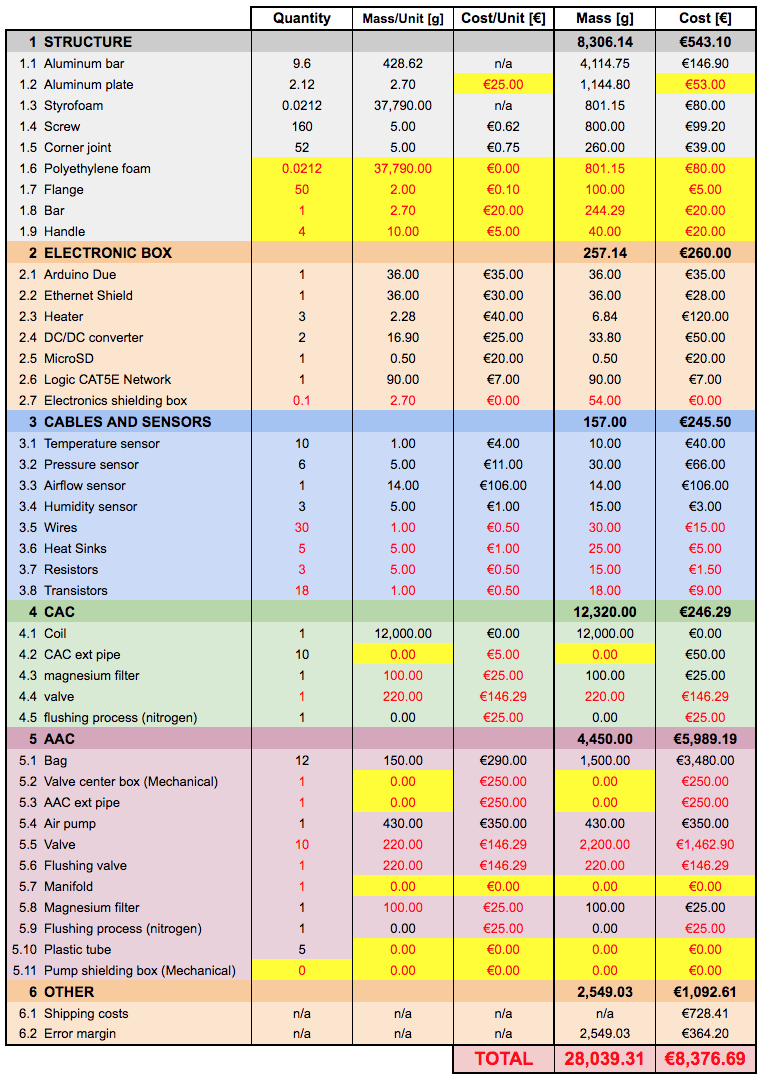
\includegraphics{3-project-planning/tables/budget-table.png}
    }\end{align*}
    %DIFAUXCMD
\DIFdelendFL \DIFaddbeginFL \centering
\begin{tabular}{l|m{0.12\textwidth}|l|r|r|r|c}
\hline
\multicolumn{1}{|l|}{\textbf{Sponsor}} & \multicolumn{1}{|c|}{\textbf{Type}} & \multicolumn{1}{c|}{\textbf{Value}} & \multicolumn{1}{c|}{\textbf{Allocated}} & \multicolumn{1}{c|}{\textbf{Unallocated}} & \multicolumn{1}{c|}{\textbf{\% Allocation}} & \multicolumn{1}{c|}{\textbf{Status}} \\ \hline
\multicolumn{1}{|l|}{LTU} & \DIFaddFL{Funds }& \DIFaddFL{2,500.00 }& \DIFaddFL{2,466.82 }& \DIFaddFL{33.18 }& \DIFaddFL{99 }& \multicolumn{1}{c|}{Received} \\ \hline
\multicolumn{1}{|l|}{SNSB} & \DIFaddFL{Funds }& \DIFaddFL{2,909.80 }& \DIFaddFL{2,840.26 }& \DIFaddFL{69.54 }& \DIFaddFL{98 }& \multicolumn{1}{c|}{Unconfirmed} \\ \hline
\multicolumn{1}{|l|}{FMI} & \DIFaddFL{Component loan }& \DIFaddFL{22,603.00 }& \DIFaddFL{22,603.00 }& \DIFaddFL{0.00 }& \DIFaddFL{100 }& \multicolumn{1}{c|}{Confirmed} \\ \hline
\multicolumn{1}{|l|}{Restek} & \DIFaddFL{Component donation }& \DIFaddFL{840.34 }& \DIFaddFL{750.00 }& \DIFaddFL{90.34 }& \DIFaddFL{89 }& \multicolumn{1}{c|}{Confirmed} \\ \hline
\multicolumn{1}{|l|}{Teknolab} & \DIFaddFL{Component donation }& \DIFaddFL{200.00 }& \DIFaddFL{200.00 }& \DIFaddFL{0.00 }& \DIFaddFL{100 }& \multicolumn{1}{c|}{Received} \\ \hline
\multicolumn{1}{|l|}{SMC} & \DIFaddFL{Component donation }& \DIFaddFL{1,440.00 }& \DIFaddFL{1,440.00 }& \DIFaddFL{0.00 }& \DIFaddFL{100 }& \multicolumn{1}{c|}{Confirmed} \\ \hline
\multicolumn{1}{|l|}{Parker} & \DIFaddFL{Component donation }& \DIFaddFL{300.00 }& \DIFaddFL{300.00 }& \DIFaddFL{0.00 }& \DIFaddFL{100 }& \multicolumn{1}{c|}{Confirmed} \\ \hline
 & \multicolumn{1}{l|}{\textbf{Total}} & \textbf{\DIFaddFL{30,793.13}} & \textbf{\DIFaddFL{30,600.08}} & \textbf{\DIFaddFL{193.05}} & \textbf{\DIFaddFL{98}} & \multicolumn{1}{l}{} \\ \cline{2-6}
\end{tabular}
\DIFaddendFL \caption{\DIFdelbeginFL \DIFdelFL{Project budget table. }\DIFdelendFL \DIFaddbeginFL \DIFaddFL{Allocation of Sponsorship Funds and Component Donation }\DIFaddendFL Values\DIFdelbeginFL \DIFdelFL{highlighted in yellow have yet to be determined/estimated}\DIFdelendFL . \DIFdelbeginFL \DIFdelFL{Number values }\DIFdelendFL \DIFaddbeginFL \DIFaddFL{Amounts }\DIFaddendFL in \DIFdelbeginFL \DIFdelFL{red have been estimated rather than determined by vendor quotes}\DIFdelendFL \DIFaddbeginFL \DIFaddFL{EUR}\DIFaddendFL .\DIFdelbeginFL \DIFdelFL{Shipping cost is estimated at 10\% of total cost. Total cost error margin is set to 5\% of projected total cost. Total mass error margin is set to 10\% of projected total mass.}\DIFdelendFL }
\DIFdelbeginFL %DIFDELCMD < \label{tab:budget-table}
%DIFDELCMD < %%%
\DIFdelendFL \DIFaddbeginFL \label{table:sponsroship-allocation}
\DIFaddendFL \end{table}


\subsubsection{External Support}

Partnership with \DIFdelbegin \DIFdel{the Finnish Meteorological Institute (FMI), and the Swedish Institute of Space Physics (IRF ) }\DIFdelend \DIFaddbegin \DIFadd{FMI, and IRF }\DIFaddend will provide the team with technical guidance in implementing the sampling system. FMI’s experience in implementing past \DIFdelbegin \DIFdel{AirCore }\DIFdelend \DIFaddbegin \DIFadd{CAC }\DIFaddend sample systems provide invaluable lessons learned towards conceptualizing, designing, and implementing the proposed AAC sampling system.

FMI is a key partner in the TUBULAR project, its scientific experts will advise and support the TUBULAR project by sharing knowledge, experience, and granting accessibility of equipment. As per the agreement shown in Appendix \ref{sec:appG}, FMI will provide the TUBULAR \DIFdelbegin \DIFdel{team }\DIFdelend \DIFaddbegin \DIFadd{Team }\DIFaddend with the AirCore stainless tube component of \DIFaddbegin \DIFadd{the }\DIFaddend CAC subsystem as well as the post-flight gas analyzer. This arrangement requires careful considerations on the placement of the experiment in order to minimize hardware damage risks. These contributions \DIFdelbegin \DIFdel{will }\DIFdelend result in significant cost savings regarding equipment and component procurement.

Daily access to LTU's Space Campus in Kiruna \DIFdelbegin \DIFdel{will expose }\DIFdelend \DIFaddbegin \DIFadd{exposes }\DIFaddend the team to scientific mentorship and expert guidance from both professors and researchers involved in the study of greenhouse gases and climate change. Dr Uwe Raffalski, \DIFdelbegin \DIFdel{Swedish institute of Space physics (IRF)}\DIFdelend \DIFaddbegin \DIFadd{IRF}\DIFaddend , Associate professor (Docent) is one of many researchers involved in climate study who is mentoring the team.
\pagebreak

\subsection{Outreach Approach}

The experiment as well as the \DIFaddbegin \DIFadd{REXUS/}\DIFaddend BEXUS programme and its partners will be promoted through the following activities:

\begin{itemize}
\item Research paper published in partnership with \DIFdelbegin \DIFdel{the Finnish Meteorological Institute (FMI ) }\DIFdelend \DIFaddbegin \DIFadd{FMI }\DIFaddend detailing the sampling methodology, measurement result, analysis, and findings.
\item Collected data will be licensed as open data to be freely available to everyone to use and republish as they wish, without restrictions from copyright, patents or other mechanisms of control.
\item A website will be launched that will summarize the experiment and provide regular updates. Backend web analytics included to gauge interest on the project through number of visitors and their origins \DIFaddbegin \DIFadd{(See Appendix \ref{sec:appE})}\DIFaddend .
\item Dedicated Facebook page used as publicly accessible logbook detailing challenges, progress, and status of the project. Open for comments and questions (See Figure \ref{fig:outreach-facebook} in Appendix \ref{sec:appE}).
\item Two Instagram accounts for short and frequent image and video focused updates. A primary Instagram account will be dedicated to project updates. A secondary account will reach out to a broader audience by focusing on space instruments in general and cross-reference TUBULAR related activities when relevant (See Figures \ref{fig:outreach-instagram}, \ref{fig:outreach-instagram-si-1}, and \ref{fig:outreach-instagram-si-2} in Appendix \ref{sec:appE}).
\item GitHub account to host all project software code under free and open source license (See \DIFdelbegin \DIFdel{Figures }\DIFdelend \DIFaddbegin \DIFadd{Figure }\DIFaddend \ref{fig:outreach-github} in Appendix \ref{sec:appE}). Other REXUS/BEXUS teams will be invited to host their code in this account in what will hopefully become a centralized GitHub account and code archive for present and future REXUS/BEXUS projects.
\item Reddit Ask Me Anything (AMA) thread to discuss the project with community of online enthusiasts.
\item\enquote{Show and Tell} trips to local high schools and universities. Team members will be responsible to organize such presentations through any of their travel opportunities abroad.
\item \DIFaddbegin \DIFadd{Articles and/or blogposts about the project in team members' alma mater websites.
}\item \DIFaddend In-booth presentation and poster display in the seminars or career events at different universities. 
\item A thoroughly documented and user-friendly manual on how to build replicate and launch CAC and AAC sampling systems will be produced and published.
\end{itemize}
\pagebreak
\subsection{Risk Register}
\textbf{Risk ID}
\begin{enumerate}[label={}]
    \item TC – \DIFdelbegin \DIFdel{technical}\DIFdelend \DIFaddbegin \DIFadd{Technical}\DIFaddend /\DIFdelbegin \DIFdel{implementation 
    }\DIFdelend \DIFaddbegin \DIFadd{Implementation 
    }\DIFaddend \item MS – \DIFdelbegin \DIFdel{mission }\DIFdelend \DIFaddbegin \DIFadd{Mission }\DIFaddend (operational performance) 
    \item SF – \DIFdelbegin \DIFdel{safety 
    }\DIFdelend \DIFaddbegin \DIFadd{Safety 
    }\DIFaddend \item VE – \DIFdelbegin \DIFdel{vehicle 
    }\DIFdelend \DIFaddbegin \DIFadd{Vehicle 
    }\DIFaddend \item PE – \DIFdelbegin \DIFdel{personnel 
    }\DIFdelend \DIFaddbegin \DIFadd{Personnel 
    }\DIFaddend \item EN – \DIFdelbegin \DIFdel{environmental 
    }\DIFdelend \DIFaddbegin \DIFadd{Environmental 
    }\DIFaddend \item OR - Outreach
    \item BG - Budget
\end{enumerate}

Adapt these to the experiment and add other categories. 
Consider risks to the experiment, to the vehicle and to personnel. 

\textbf{Probability (P)}
\begin{enumerate}[label=\Alph*]
    \item Minimum – Almost impossible to occur 
    \item Low – Small chance to occur 
    \item Medium – Reasonable chance to occur 
    \item High – Quite likely to occur 
    \item Maximum – Certain to occur, maybe more than once
\end{enumerate}

\textbf{Severity (S)}
\begin{enumerate}
    \item Negligible – Minimal or no impact 
    \item Significant – Leads to reduced experiment performance 
    \item Major – Leads to failure of subsystem or loss of flight data 
    \item Critical – Leads to experiment failure or creates minor health hazards 
    \item Catastrophic – Leads to termination of the \DIFaddbegin \DIFadd{REXUS/}\DIFaddend BEXUS programme, damage to the vehicle or injury to personnel 
\end{enumerate}

The rankings for probability (P) and severity (S) are combined to assess the overall risk classification, ranging from very low to very high and being coloured green, yellow, orange or red according to the SED guidelines.

\begin{landscape}
\DIFaddbegin 



\DIFaddend \begin{longtable}{|m{0.09\textwidth}| m{0.51\textwidth} |m{0.03\textwidth} |m{0.03\textwidth}|m{0.11\textwidth}| m{0.65\textwidth}|}

\hline
\textbf{ID} & \textbf{Risk (\& consequence if)} & \textbf{P} & \textbf{S} & \textbf{P * S} & \textbf{Action} \\ \hline
TC10 & Software fails to store data & B & \DIFdelbegin \DIFdel{4 }\DIFdelend \DIFaddbegin \DIFadd{3 }\DIFaddend & \cellcolor[HTML]{FCFF2F}Low & Acceptable Risk: Extensive testing will be done\DIFaddbegin \DIFadd{. Using telemetry, all data gathered from sensors will be sent to ground station. }\DIFaddend \\ \hline
TC20 & Failure of several sensors & B & \DIFdelbegin \DIFdel{3 }\DIFdelend \DIFaddbegin \DIFadd{4 }\DIFaddend & \cellcolor[HTML]{FCFF2F}Low & Acceptable Risk: Thermal test \DIFaddbegin \DIFadd{(Test Number 5) }\DIFaddend to approve the functionality of the experiment. \\ \hline
TC30 & Critical component is destroyed in testing & B & 1 & \cellcolor[HTML]{FCFF2F}Low & Acceptable risk: Spare components can be ordered but for expensive ones, they will be ordered and tested early in the project in case we need to order more. \\ \hline
TC40 & Electrical connections dislodges or short circuits because of vibration or shock & B & 3 & \cellcolor[HTML]{FCFF2F}Low & Unacceptable risk. \DIFaddbegin \DIFadd{D-sub connections will be screwed in place. It will be ensured that there are no loose connections and zip ties will be used to help keep wires in place. }\DIFaddend Careful soldering and extensive testing will be applied. \\ \hline
TC50 & Experiment electronics fail due to long exposure to cold or warm temperatures & B & 3 & \cellcolor[HTML]{FCFF2F}Low & Unacceptable Risk: Thermomechanical and thermoelectrical solutions will be simulated and tested in detail to help prevent this from happening. \\ \hline
TC60 & Software and electrical fail to control heaters causing temperature to drop or rise below or above operational range & B & 2 & \cellcolor[HTML]{34FF34}Very Low & Unacceptable risk: Tests will be performed prior to the flight to detect and minimize the risk of occurrence.The system will be monitored during flight and handled manually if necessary. \\ \hline
TC70 & Software fails to enter safe mode (may result in loss of data) & B & 3 & \cellcolor[HTML]{FCFF2F}Low & Acceptable Risk: Extensive testing will be done. \\ \hline
TC80 & On-board memory will be full (flight time longer than expected) & A & 2 & \cellcolor[HTML]{34FF34}Very Low & Acceptable Risk: The experiment shall go through testing and analysis to guarantee the onboard memory size is sufficient.\\ \hline
TC90 & Connection loss with ground station & A & 4 & \cellcolor[HTML]{34FF34}Very Low & Acceptable Risk: Experiment will be designed to operate autonomously. \\ \hline
TC100 & Software fails to control valves autonomously & B & 4 & \cellcolor[HTML]{FCFF2F}Low & Acceptable Risk: Extensive testing will be done. Telecommand will also be used to manually control the valves. \\ \hline
TC110 & Software fails to change modes autonomously & B & 4 & \cellcolor[HTML]{FCFF2F}Low & Acceptable Risk: Extensive testing will be done. Telecommand will also be used to manually change experiment modes. \\ \hline
TC120 & Complete software failure & B & 4 & \cellcolor[HTML]{FCFF2F}Low & Acceptable Risk: \DIFdelbegin \DIFdel{Watchdog timer will be applied to reset software if it freezes}\DIFdelend \DIFaddbegin \DIFadd{A long duration testing (bench test) will be performed to catch the failures early}\DIFaddend . \\ \hline
TC130 & Failure of fast \DIFdelbegin \DIFdel{opening }\DIFdelend \DIFaddbegin \DIFadd{recovery }\DIFaddend system & B & 2 & \cellcolor[HTML]{34FF34}Very Low & Acceptable risk: \DIFdelbegin \DIFdel{the box could also be opened but a little bit slower. }\DIFdelend \DIFaddbegin \DIFadd{Clear and simple instructions will be given to the recovery team. A test will take place before launch to ensure someone unfamiliar with the experiment can remove the CAC box. Test number: 12. }\DIFaddend \\ \hline
TC140 & The gas analyzer isn't properly calibrated and returns inaccurate results & B & 4 & \cellcolor[HTML]{FCFF2F}Low & Acceptable risk: Calibrate the gas analyzer before use.\\ \hline
\DIFaddbegin \DIFadd{TC150 }& \DIFadd{Partnership with FMI does not materialize, resulting in loss of access to CAC coiled tube. }& \DIFadd{B }& \DIFadd{2 }& \cellcolor[HTML]{34FF34}\DIFadd{Very Low }& \DIFadd{Acceptable Risk: Signed agreement has been obtained. AAC sample analysis results can be validated against available historical data from past FMI CAC flights. }\\ \hline 
\DIFaddend MS10 & Down link connection is lost prematurely & B & 2 & \cellcolor[HTML]{34FF34}Very Low & Acceptable Risk: Data will also be saved on SD card. \\ \hline
MS20 & Condensation on experiment PCBs which could causes short circuits & A & 3 & \cellcolor[HTML]{34FF34}Very Low & Acceptable risk: \DIFdelbegin \DIFdel{Circuit box }\DIFdelend \DIFaddbegin \DIFadd{The Brain }\DIFaddend will be sealed to prevent condensation. \\ \hline
MS30 & Temperature sensitive components that are essential to full the mission objective might be below their operating temperature. & C & 3 & \cellcolor[HTML]{FCFF2F}Low & Acceptable Risk: Safe mode to prevent the components to operate out of its operating temperature range. \\ \hline
MS40 & Experiment lands in water causing electronics failure & B & 1 & \cellcolor[HTML]{34FF34}Very Low & Acceptable risk: Check if SD card needs waterproof shell or is waterproof in itself. Also, all the necessary data will be downloaded during the flight. \\ \hline
MS50 & Interference from other experiments and/or balloon & A & 4 & \cellcolor[HTML]{34FF34}Very Low & Acceptable risk: no action. \\ \hline
MS60 & Balloon power failure & C & \DIFdelbegin \DIFdel{1 }\DIFdelend \DIFaddbegin \DIFadd{2 }\DIFaddend & \cellcolor[HTML]{34FF34}Very Low & Acceptable risk: Valves default state is closed so if all power is lost valves will automatically close preserving all samples collected up until that point. \\ \hline
MS70 & \DIFdelbegin \DIFdel{Bags }\DIFdelend \DIFaddbegin \DIFadd{Sampling bags }\DIFaddend disconnect & C & 3 & \cellcolor[HTML]{FCFF2F}Low & Acceptable Risk: The affected bags could not collect samples. A proper fixing of the flanges must be double checked.
\\ \hline
MS71 & \DIFdelbegin \DIFdel{Bags }\DIFdelend \DIFaddbegin \DIFadd{Sampling bags }\DIFaddend puncture & B & 3 & \cellcolor[HTML]{FCFF2F}Low & Acceptable Risk: The affected bags could not collect samples. Proper protection will be placed in order to avoid puncture from external elements. \\ \hline
MS72 & \DIFdelbegin \DIFdel{Bags}\DIFdelend \DIFaddbegin \DIFadd{Sampling bags}\DIFaddend ' hold time is typically 48h & C & 3 & \cellcolor[HTML]{FCFF2F}Low & Acceptable risk: Validation studies can demonstrate longer stability.  \\ \hline
MS80 & Pump failure & \DIFdelbegin \DIFdel{C }\DIFdelend \DIFaddbegin \DIFadd{B }\DIFaddend & 4 & \DIFdelbegin %DIFDELCMD < \cellcolor[HTML]{ffae42}%%%
\DIFdel{Medium }\DIFdelend \DIFaddbegin \cellcolor[HTML]{FCFF2F}\DIFadd{Low }\DIFaddend & Unacceptable risk: \DIFdelbegin \DIFdel{The bags would not be filled and thus the AAC system would fail. The pump will be properly }\DIFdelend \DIFaddbegin \DIFadd{A pump was }\DIFaddend chosen based on \DIFdelbegin \DIFdel{past research and extensively tested before the flight}\DIFdelend \DIFaddbegin \DIFadd{a previous similar experiment. The pump has also been tested in a low pressure chamber down to 10hPa and has successfully turned on and filled a sampling bag}\DIFaddend . \\ \hline
MS90 & Intake pipe blocked by external element & C & 3 & \cellcolor[HTML]{FCFF2F}Low & Unacceptable Risk: The bags would not be filled and thus the AAC system would fail. An air filter will be placed in both intake and outlet of the pipe to prevent this. \\ \hline
\DIFaddbegin \DIFadd{MS100 }& \DIFadd{Expansion/Contraction of insulation }& \DIFadd{B }& \DIFadd{2 }&\cellcolor[HTML]{34FF34}\DIFadd{Very Low }& \DIFadd{Acceptable Risk: The insulation selected has flown successfully on similar flights in the past. Test shall be done to see how it reacts in a low pressure environment. }\\ \hline
\DIFadd{MS110 }& \DIFadd{Sampling bags are over-filled resulting in bursting and loss of collected samples. }& \DIFadd{B }& \DIFadd{3 }& \cellcolor[HTML]{FCFF2F}\DIFadd{Low }& \DIFadd{Unacceptable Risk: Test will be performed at target ambient pressure levels to identify how long the pump needs to fill the sampling bags. Pressure sensors on board will monitor the in bag pressure during sampling and no bag will ever be over pressured. }\\ \hline 
\DIFaddend VE10 & SD-card is destroyed at impact & B & \DIFdelbegin \DIFdel{3 }\DIFdelend \DIFaddbegin \DIFadd{2 }\DIFaddend & \DIFdelbegin %DIFDELCMD < \cellcolor[HTML]{FCFF2F}%%%
\DIFdelend \DIFaddbegin \cellcolor[HTML]{34FF34}\DIFadd{Very }\DIFaddend Low & Acceptable Risk: All data will be transmitted to the ground. \DIFaddbegin \DIFadd{Most of the data is the gas stored in the AAC and CAC. }\DIFaddend \\ \hline
VE20 & Gondola Fixing Interface & B & 4 & \cellcolor[HTML]{FCFF2F}Low & Unacceptable Risk: The experiment box could detach from the gondola’s rails and the two boxes could detach one from the other. Proper fixing has been designed to prevent it. \\ \hline
VE30 & Structure damage due to bad landing & B & 3 & \cellcolor[HTML]{FCFF2F}Low & Acceptable Risk: Landing directly on a hard element could break the structure or the protective walls. Consistent design implemented to prevent it. \\ \hline
VE40 & Hard landing damages the CAC equipment & C & 3 & \cellcolor[HTML]{FCFF2F}Low & Acceptable risk:  Proper  protection will be placed in order to avoid damage from hard landing. \\ \hline
VE50 & Hard landing damages the AAC equipment & C & 3 & \cellcolor[HTML]{FCFF2F}Low & Acceptable risk:  Proper  protection will be placed in order to avoid puncture from hard landing. \\ \hline
EN10 & Vibrations & C & 1 & \cellcolor[HTML]{34FF34}Very Low & Acceptable risk: Vibrations do not affect the sampled air. \\ \hline
EN20 & The air samples must be protected from direct sunlight and stored above 0 \degree C to prevent condensation & \DIFdelbegin \DIFdel{D }\DIFdelend \DIFaddbegin \DIFadd{C }\DIFaddend & \DIFdelbegin \DIFdel{4 }\DIFdelend \DIFaddbegin \DIFadd{3 }\DIFaddend & \DIFdelbegin %DIFDELCMD < \cellcolor[HTML]{FF0800}%%%
\DIFdel{High risk }\DIFdelend \DIFaddbegin \cellcolor[HTML]{FCFF2F}\DIFadd{Low }\DIFaddend & \DIFdelbegin \DIFdel{Unacceptable risk: Further test regarding insulation performance and humidity levels in the bags will be done}\DIFdelend \DIFaddbegin \DIFadd{Acceptable risk: Stratospheric air is generally dry and water vapor concentrations are higher closer to the surface. In addition magnesium perchlorate dryers will be used to minimizing the risk of condensation}\DIFaddend .    \\ \hline 
PE10 & \DIFdelbegin \DIFdel{The Project Manager is no longer available to manage the project}\DIFdelend \DIFaddbegin \DIFadd{Change in Project Manager after the CDR introduces a gap of knowledge in management responsibilities}\DIFaddend . & E & 1 & \cellcolor[HTML]{FCFF2F}Low & Acceptable risk: \DIFdelbegin \DIFdel{The }\DIFdelend \DIFaddbegin \DIFadd{A }\DIFaddend Deputy Project Manager \DIFdelbegin \DIFdel{will take over as Project Manager . }\DIFdelend \DIFaddbegin \DIFadd{is selected at an early stage and is progressively handed over project management tasks and responsibilities until complete handover after the CDR. The previous Project Manager remotely assists the new Project Manager until the end of the project. The Deputy Project Manager is also part of the Electrical Division so a new team member has been included to that division in order compensate for the Deputy Project Manager's reduced bandwidth to work on Electrical Division tasks once she is appointed Project Manager.}\DIFaddend \\ \hline 
PE20 & Team members from the same division are unavailable during the same period over the summer. & C & \DIFdelbegin \DIFdel{4 }\DIFdelend \DIFaddbegin \DIFadd{3 }\DIFaddend & \DIFdelbegin %DIFDELCMD < \cellcolor[HTML]{ffae42}%%%
\DIFdel{Medium risk }\DIFdelend \DIFaddbegin \cellcolor[HTML]{FCFF2F}\DIFadd{Low }\DIFaddend & Unacceptable risk: Summer travel schedules \DIFdelbegin \DIFdel{to be }\DIFdelend \DIFaddbegin \DIFadd{have been }\DIFaddend coordinated among team members \DIFdelbegin \DIFdel{and approved by Project Manager}\DIFdelend \DIFaddbegin \DIFadd{so that there is at least one member from each division available during the summer}\DIFaddend . \\ \hline
% & & & & &\\ \hline

%\end{tabular}
\caption{Risk Register}
\label{tab:risk-register}
\end{longtable}
\raggedbottom
\end{landscape}

\pagebreak
\section{Experiment Design}
\subsection{Experiment Setup} \label{Experiment_Setup}

The experiment consists of \DIFdelbegin \DIFdel{AAC ten sampling bagssubsystem}\DIFdelend \DIFaddbegin \DIFadd{the AAC subsystem, with six sampling bags}\DIFaddend , and the CAC coiled tube subsystem. \DIFaddbegin \DIFadd{Shown in Figure }{\DIFadd{\ref{fig:3D_tubular_render}}}\DIFadd{, the CAC is fitted into the partition on the left, and the AAC into the partition to the right. }\DIFaddend The principal aim is to validate the AAC sampling method\DIFdelbegin \DIFdel{and to }\DIFdelend \DIFaddbegin \DIFadd{. To }\DIFaddend do so, it is necessary to sample during \DIFdelbegin \DIFdel{descent phase }\DIFdelend \DIFaddbegin \DIFadd{Descent Phase }\DIFaddend in order to compare the results with the ones obtained from the CAC. \DIFdelbegin \DIFdel{All }\DIFdelend \DIFaddbegin \DIFadd{This is because the CAC collects its air sample passively by pressure differentials in the descent. Flight }\DIFaddend speeds mentioned in this section have been obtained from the BEXUS manual as well as through analysis of past flights. \DIFaddbegin \DIFadd{Figure \ref{fig:block-diagram} shows a generic block diagram of the main subsystems interconnection.
}\DIFaddend 

\DIFaddbegin \begin{figure}[H]
    \begin{align*}
        \DIFaddFL{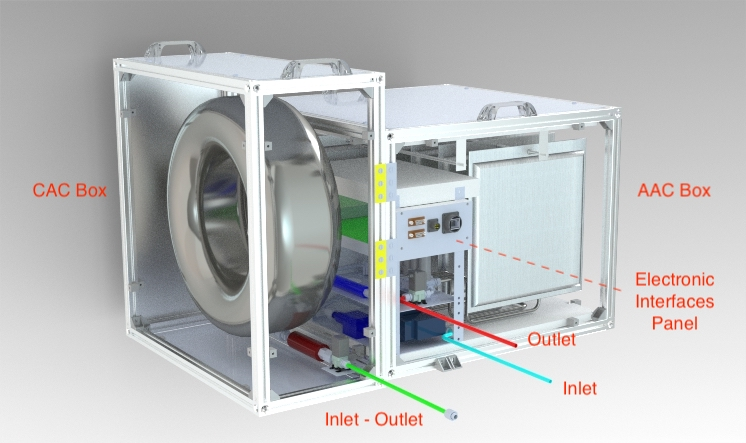
\includegraphics[width=1\linewidth]{4-experiment-design/img/Mechanical/v9_3D.jpg}
    }\end{align*}
    \caption{\DIFaddFL{Physical setup of the experiment.}}
    \label{fig:3D_tubular_render}
\end{figure}

\begin{figure}[H]
    \begin{align*}
        \DIFaddFL{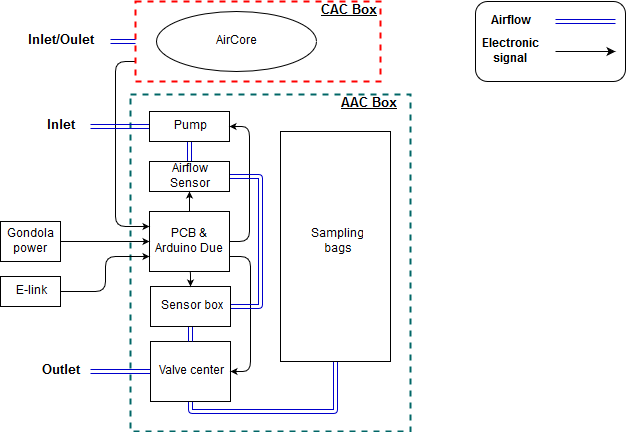
\includegraphics[width=1\linewidth]{4-experiment-design/img/Mechanical/Block-Diagram.png}
    }\end{align*}
    \caption{\DIFaddFL{Block diagram of the experiment.}\label{fig:block-diagram}}
\end{figure}

\DIFaddend The primary concern regarding the AAC air sampling subsystem \DIFdelbegin \DIFdel{is that after }\DIFdelend \DIFaddbegin \DIFadd{occurs after the }\DIFaddend cut-off \DIFaddbegin \DIFadd{when }\DIFaddend the gondola will tumble and fall at an average speed of 50 m/s for approximately \DIFdelbegin \DIFdel{2 }\DIFdelend \DIFaddbegin \DIFadd{two }\DIFaddend minutes \cite{BexusManual}. This \DIFdelbegin \DIFdel{falling }\DIFdelend \DIFaddbegin \DIFadd{descent }\DIFaddend speed is too \DIFdelbegin \DIFdel{fast }\DIFdelend \DIFaddbegin \DIFadd{large }\DIFaddend in order to sample air at the desired vertical resolution\DIFdelbegin \DIFdel{that is targeted to be 500m. This means that only }\DIFdelend \DIFaddbegin \DIFadd{, capped at 500 m. As such, sampling can only be done }\DIFaddend after the gondola \DIFdelbegin \DIFdel{is }\DIFdelend \DIFaddbegin \DIFadd{has }\DIFaddend stabilized at a descent \DIFdelbegin \DIFdel{rate }\DIFdelend \DIFaddbegin \DIFadd{speed  }\DIFaddend of 8 m/s \cite{BexusManual}\DIFdelbegin \DIFdel{the sampling can be done}\DIFdelend . The tumbling phase will \DIFdelbegin \DIFdel{span approximately for 6km and considering a floating phase at 25km, the sampling can be started from 19km }\DIFdelend \DIFaddbegin \DIFadd{vertically span for approximately 6 km. Considering a Float Phase altitude of 25 km, sampling during the Descent Phase will commence at approximately 19 km }\DIFaddend in altitude. \DIFdelbegin \DIFdel{Nevertheless, the main }\DIFdelend \DIFaddbegin \DIFadd{However, the primary }\DIFaddend region of interest \DIFdelbegin \DIFdel{is }\DIFdelend \DIFaddbegin \DIFadd{in terms of sampling is in }\DIFaddend the stratosphere, \DIFdelbegin \DIFdel{especially between 19km and 25km of altitude. It is for this reason that the team has decided to sample during ascent phase as well. Ten sampling bags will be filled up, six during ascent phase approximately between 18-24km, and four during descent phase below 19km. The desired vertical resolution is 500 m at a falling speed of 8 m/s which means that using bags with a volume of 3L, an air pump with at least 3L/min intake rate is necessary for the sampling bags}\DIFdelend \DIFaddbegin \DIFadd{particularly between 19 km and 25 km in altitude. Sampling will thus also occur during the Ascent Phase. Out of the six sampling bags present in the payload, two will be used during the Ascent Phase at 18 km and 21 km and four during the Descent Phase at 17.5 km, 16 km, 14 km and 12 km as seen in Table \ref{tab:sampling-altitudes}. Details regarding the sampling strategy can be found in Appendix \ref{sec:appH}}\DIFaddend .


\DIFaddbegin \begin{table}[H]
\centering
\begin{tabular}{|c|c|c|c|}
\hline
\multicolumn{1}{|l|}{} & \multicolumn{1}{l|}{\textbf{Sampling Altitudes}} & \multicolumn{1}{l|}{\textbf{Ambient Pressure}} & \multicolumn{1}{l|}{\textbf{Ambient Temperature}} \\ \hline
\multirow{2}{*}{\textbf{Ascent Phase}} & \DIFaddFL{18 km }& \DIFaddFL{75.0 hPa }& \DIFaddFL{216.7 K }\\ \cline{2-4} 
 & \DIFaddFL{21 km }& \DIFaddFL{46.8 hPa }& \DIFaddFL{217.6 K }\\ \hline
\multirow{4}{*}{\textbf{Descent Phase}} & \DIFaddFL{17.5 km }& \DIFaddFL{81.2 hPa }& \DIFaddFL{216.7 K }\\ \cline{2-4} 
 & \DIFaddFL{16 km }& \DIFaddFL{102.9 hPa }& \DIFaddFL{216.7 K }\\ \cline{2-4} 
 & \DIFaddFL{14 km }& \DIFaddFL{141.0 hPa }& \DIFaddFL{216.7 K }\\ \cline{2-4} 
 & \DIFaddFL{12 km }& \DIFaddFL{193.3 hPa }& \DIFaddFL{216.7 K }\\ \hline
\end{tabular}
\caption{\DIFaddFL{Sampling Altitudes as well as the Corresponding Ambient Pressures and Temperatures According to the 1976 US Standard Atmosphere}}
\label{tab:sampling-altitudes}
\end{table}

\DIFaddend The maximum pressure that the sampling bags can withstand has to be taken into account in order to avoid bursting. \DIFdelbegin \DIFdel{During ascent phase, due to the decreasing pressure , the bags with the air samples , }\DIFdelend \DIFaddbegin \DIFadd{Decreasing pressure during the Ascent Phase poses a risk to sampling bags which already contain samples as the gas inside }\DIFaddend will expand which may \DIFdelbegin \DIFdel{have risk of bursting. To }\DIFdelend \DIFaddbegin \DIFadd{cause the bag to burst. In order to }\DIFaddend avoid this, the \DIFdelbegin \DIFdel{bags should not be fully sampled. The providers recommend not to fill more than }\DIFdelend \DIFaddbegin \DIFadd{sampling bags will not be completely filled. Filling up to a maximum of }\DIFaddend 80\% \DIFdelbegin \DIFdel{(~2psi}\DIFdelend \DIFaddbegin \DIFadd{of the sampling bag's capacity (2 psi}\DIFaddend /0.14 bar) \DIFdelbegin \DIFdel{for }\DIFdelend \DIFaddbegin \DIFadd{is recommended by the manufacturers for the }\DIFaddend Multi-Layer Foil \DIFdelbegin \DIFdel{bags. The opposite applies for descent phase. The bags with the air samples, will be compressed, and }\DIFdelend \DIFaddbegin \DIFadd{sampling bags that are to be used. The inverse is also true for the Descent Phase where compression will occur. As such, the sampling bags should be fully filled during the Descent Phase }\DIFaddend in order to \DIFdelbegin \DIFdel{assure that the samples are enough for analysis, they should be fully filled. It has to be mentioned that it has been found from past research \mbox{%DIFAUXCMD
\cite{LISA} }\hspace{0pt}%DIFAUXCMD
that the same }\DIFdelend \DIFaddbegin \DIFadd{ensure that enough samples are collected for analysis. Past research has revealed that the selected sampling }\DIFaddend bags can withstand \DIFdelbegin \DIFdel{a difference in pressure between outside and inside of 310hPa at 30km }\DIFdelend \DIFaddbegin \DIFadd{pressure difference of 310 hPa at 30 km }\DIFaddend of altitude, which is equivalent to 0.31 bar \DIFdelbegin \DIFdel{. Therefore, future test will }\DIFdelend \DIFaddbegin \DIFadd{\mbox{%DIFAUXCMD
\cite{LISA}}\hspace{0pt}%DIFAUXCMD
. A series of tests listed in Table \ref{tab:sampling-system-test} will be conducted in order to }\DIFaddend confirm the maximum \DIFaddbegin \DIFadd{allowable }\DIFaddend pressure for the bags.


\DIFdelbegin \DIFdel{Depending on the altitude of sampling , the range }\DIFdelend \DIFaddbegin \DIFadd{Due to the difference in pressure between sea level and sampling altitudes, the volume }\DIFaddend of the sample \DIFdelbegin \DIFdel{size is between 0.2L and 0.8L, with 0.2L being the minimum amount }\DIFdelend \DIFaddbegin \DIFadd{taken will be considerably reduced when it reaches sea level. This shrinking has to be taken into account as the minimum volume that has to be present in the sampling bag at ground level in order to obtain results with the Picarro analyzer. A minimum amount is }\DIFaddend required for the \DIFdelbegin \DIFdel{chromatographer to analyze. }\DIFdelend \DIFaddbegin \DIFadd{analyzer to detect concentrations of the targeted trace gases. This minimum amount is 0.18 L at sea level and it has to be specially considered for the samples taken at higher altitudes. The samples taken at lower altitudes will be exposed to smaller changes in pressure, therefore their size will not be critically reduced. Table \ref{tab:minimum-volume} shows the minimum volume of air that needs to be sampled at different altitudes, in order the sample volume left at sea level pressure is at least 0.18L..  
}\DIFaddend 

%DIF >  Depending on the sampling altitude,there is a minimum volume of air that needs to be sampled in order the sample volume left at sea level pressure is at least 0.18 L. A sample volume of 0.18 L corresponds to the minimum amount required for the Picarro analyzer to detect concentrations of the targeted trace gases. 
\DIFaddbegin 

%DIF >  Please add the following required packages to your document preamble:
%DIF >  \usepackage{multirow}
\begin{table}[H]
\centering
\begin{tabular}{|l|l|l|l|l|}
\hline
 & \textbf{\begin{tabular}[c]{@{}l@{}}\DIFaddFL{Minimum }\\ \DIFaddFL{Sampling Volume}\end{tabular}} & \textbf{\begin{tabular}[c]{@{}l@{}}\DIFaddFL{Sampling }\\ \DIFaddFL{Altitudes}\end{tabular}} & \textbf{\begin{tabular}[c]{@{}l@{}}\DIFaddFL{Ambient }\\ \DIFaddFL{Pressure}\end{tabular}} & \textbf{\begin{tabular}[c]{@{}l@{}}\DIFaddFL{Ambient }\\ \DIFaddFL{Temperature}\end{tabular}} \\ \hline
\multirow{2}{*}{\textbf{Ascent Phase}} & \DIFaddFL{1.8 L }& \DIFaddFL{18 km }& \DIFaddFL{75.0 hPa }& \DIFaddFL{216.7 K }\\ \cline{2-5} 
 & \DIFaddFL{2.4 L }& \DIFaddFL{21 km }& \DIFaddFL{46.8 hPa }& \DIFaddFL{217.6 K }\\ \hline
\multirow{4}{*}{\textbf{Descent Phase}} & \DIFaddFL{1.7 L }& \DIFaddFL{17.5 km }& \DIFaddFL{81.2 hPa }& \DIFaddFL{216.7 K }\\ \cline{2-5} 
 & \DIFaddFL{1.3 L }& \DIFaddFL{16 km }& \DIFaddFL{102.9 hPa }& \DIFaddFL{216.7 K }\\ \cline{2-5} 
 & \DIFaddFL{1.0 L }& \DIFaddFL{14 km }& \DIFaddFL{141.0 hPa }& \DIFaddFL{216.7 K }\\ \cline{2-5} 
 & \DIFaddFL{0.7 L }& \DIFaddFL{12 km }& \DIFaddFL{193.3 hPa }& \DIFaddFL{216.7 K }\\ \hline
\end{tabular}
\caption{\DIFaddFL{Minimum Sampling Volume at Each Altitude to Obtain Enough Air to Perform a Proper Analysis (0.18 L at sea level), Appendix \ref{sec:appH}}}
\label{tab:minimum-volume}
\end{table}


\DIFaddend The AAC will need an air pump for sampling \DIFdelbegin \DIFdel{, }\DIFdelend due to low ambient pressure at stratospheric altitudes. The air pump is also needed in order to assure the intake flow rate and obtain a good resolution. \DIFdelbegin \DIFdel{A control }\DIFdelend \DIFaddbegin \DIFadd{An air pump with an intake rate of at least 3 L/min will be used to ensure that the vertical resolution of the sampling air remains under 500 m during the Ascent Phase's ascent speed of 5 m/s and the  Descent Phase's descent speed of 8 m/s. A flushing }\DIFaddend valve will be used to flush the \DIFdelbegin \DIFdel{pump after }\DIFdelend \DIFaddbegin \DIFadd{AAC system before }\DIFaddend each bag is filled and make sure that \DIFdelbegin \DIFdel{the next }\DIFdelend \DIFaddbegin \DIFadd{each }\DIFaddend bag will be filled with fresh air from the corresponding altitude. \DIFdelbegin \DIFdel{Each sampling bag will be assigned a 500 meter altitude sampling range from which to collect air samples. At an ascent speed of 5 m}\DIFdelend \DIFaddbegin \DIFadd{This filling}\DIFaddend /\DIFdelbegin \DIFdel{s }\DIFdelend \DIFaddbegin \DIFadd{flushing procedure occurs twice, the first time }\DIFaddend during the Ascent Phase \DIFdelbegin \DIFdel{and at a descent speed of 8 m/s }\DIFdelend \DIFaddbegin \DIFadd{for the first two sampling bags and the second time }\DIFaddend during the Descent Phase \DIFaddbegin \DIFadd{for the remaining four sampling bags}\DIFaddend .

Shortly after the launch, the CAC valve will be opened in order to allow \DIFdelbegin \DIFdel{flushing the inert }\DIFdelend \DIFaddbegin \DIFadd{the fill }\DIFaddend gas that is inside the tube \DIFaddbegin \DIFadd{to flush}\DIFaddend , while the AAC valves will be closed until reaching the sampling altitude. Flushing of the CAC tube happens passively through the progressive decrease in air pressure during the balloon's \DIFdelbegin \DIFdel{ascent phase. }\DIFdelend \DIFaddbegin \DIFadd{Ascent Phase and it will be emptied by the time it reaches the Float Phase. Filling of the CAC tube also happens passively through the progressive increase in air pressure during the balloon's Descent Phase. }\DIFaddend The CAC valve will remain open at all time during \DIFdelbegin \DIFdel{ascent, floating, and descent }\DIFdelend \DIFaddbegin \DIFadd{the Ascent, Float, and Descent }\DIFaddend phases. The \DIFdelbegin \DIFdel{tube will empty itself due to pressure gradient during the ascent phase and it will be filled passively during descent. The }\DIFdelend valve will close just \DIFdelbegin \DIFdel{after }\DIFdelend \DIFaddbegin \DIFadd{before }\DIFaddend hitting the ground in order to preserve the sample. 
\DIFdelbegin \DIFdel{The AAC will need an air pump for sampling, due to low ambient pressure. The air pump is also needed in order to assure the intake flow rate and obtain a good resolution.
}\DIFdelend 

\DIFdelbegin \DIFdel{After sampling for a given bag is complete, the pump will be flushed and prior to the subsequent sampling bag valve being opened. This process continues until the last sampling bag is filled.This procedure occurs twice, the first time during the Ascent Phase for the 6 first sampling bags and the second time during the descent phase for the remaining 4 sampling bags.
}%DIFDELCMD < 

%DIFDELCMD < %%%
\DIFdelend The ambient pressure will be measured by three pressure sensors located \DIFdelbegin \DIFdel{inside }\DIFdelend \DIFaddbegin \DIFadd{outside }\DIFaddend the experiment box. Only one of them is necessary for AAC and CAC, but \DIFdelbegin \DIFdel{three sensors will be used for redundancyreasons. The pressure inside the AirCore is assumed to be the same as the ambient pressure, therefore no sensor is needed. }\DIFdelend \DIFaddbegin \DIFadd{using three will provide redundancy. }\DIFaddend To measure the pressure inside the \DIFdelbegin \DIFdel{bags}\DIFdelend \DIFaddbegin \DIFadd{bag that is currently being filled}\DIFaddend , three more sensors will be allocated inside the \DIFdelbegin \DIFdel{valve center}\DIFdelend \DIFaddbegin \DIFadd{sensors box}\DIFaddend . To measure \DIFaddbegin \DIFadd{the }\DIFaddend ambient temperature in the \DIFdelbegin \DIFdel{AirCore}\DIFdelend \DIFaddbegin \DIFadd{CAC}\DIFaddend , three sensors will be allocated in the \DIFdelbegin \DIFdel{styrofoam whereas three more for the bags will be placed in the valve center}\DIFdelend \DIFaddbegin \DIFadd{CAC box (in the Styrofoam)}\DIFaddend . Temperature inside the \DIFdelbegin \DIFdel{bags/AirCore }\DIFdelend \DIFaddbegin \DIFadd{coil }\DIFaddend is assumed to quickly adjust to the ambient temperature \DIFaddbegin \DIFadd{inside the CAC box}\DIFaddend , therefore there will not be differentiation in \DIFdelbegin \DIFdel{between inside/outside temperature . }\DIFdelend \DIFaddbegin \DIFadd{temperature between the air inside the tube and the air surrounding the tube. For the bags three more temperature sensors will be placed in the bags' box (in the Styrofoam). To control the temperature for the Arduino, the pump and the valves in the Brain, one temperature sensor will be used for each of them. }\DIFaddend In total, there will be six pressure sensors and \DIFdelbegin \DIFdel{six }\DIFdelend \DIFaddbegin \DIFadd{nine }\DIFaddend temperature sensors. 

The sampling of the AAC will be triggered by the pressure reading from the sensors \DIFdelbegin \DIFdel{inside the valve center}\DIFdelend \DIFaddbegin \DIFadd{outside the experiment box}\DIFaddend . When the required pressure is reached, \DIFdelbegin \DIFdel{the valve }\DIFdelend \DIFaddbegin \DIFadd{Table \ref{tab:sampling-altitudes} the valve inside the manifold corresponding to the bag that is to be sampled, }\DIFaddend will open and the sampling will start. The closing of the valve depends on two conditions and it will be triggered when either one of the conditions is true. These conditions are: maximum sampling time or maximum pressure difference between inside/outside the bags. They are determined from past research \DIFdelbegin \DIFdel{but }\DIFdelend \DIFaddbegin \DIFadd{\mbox{%DIFAUXCMD
\cite{LISA}}\hspace{0pt}%DIFAUXCMD
. A first estimation of the maximum sampling time has already been made, from Test 18 shown in Table \ref{tab:pump-low-pressure-test}, but more tests }\DIFaddend in the future will \DIFdelbegin \DIFdel{be determined by testing}\DIFdelend \DIFaddbegin \DIFadd{determine the maximum pressure condition and confirm the maximum sampling times}\DIFaddend .

The \DIFdelbegin \DIFdel{emptying and }\DIFdelend \DIFaddbegin \DIFadd{CAC emptying as well as the AAC and CAC }\DIFaddend sampling sequence is represented in Figures \ref{fig:ascent} and \ref{fig:descent}. It should be kept in mind that the different pressures are what triggers the opening of the valves. 

\begin{figure}[H]
    \begin{align*}
        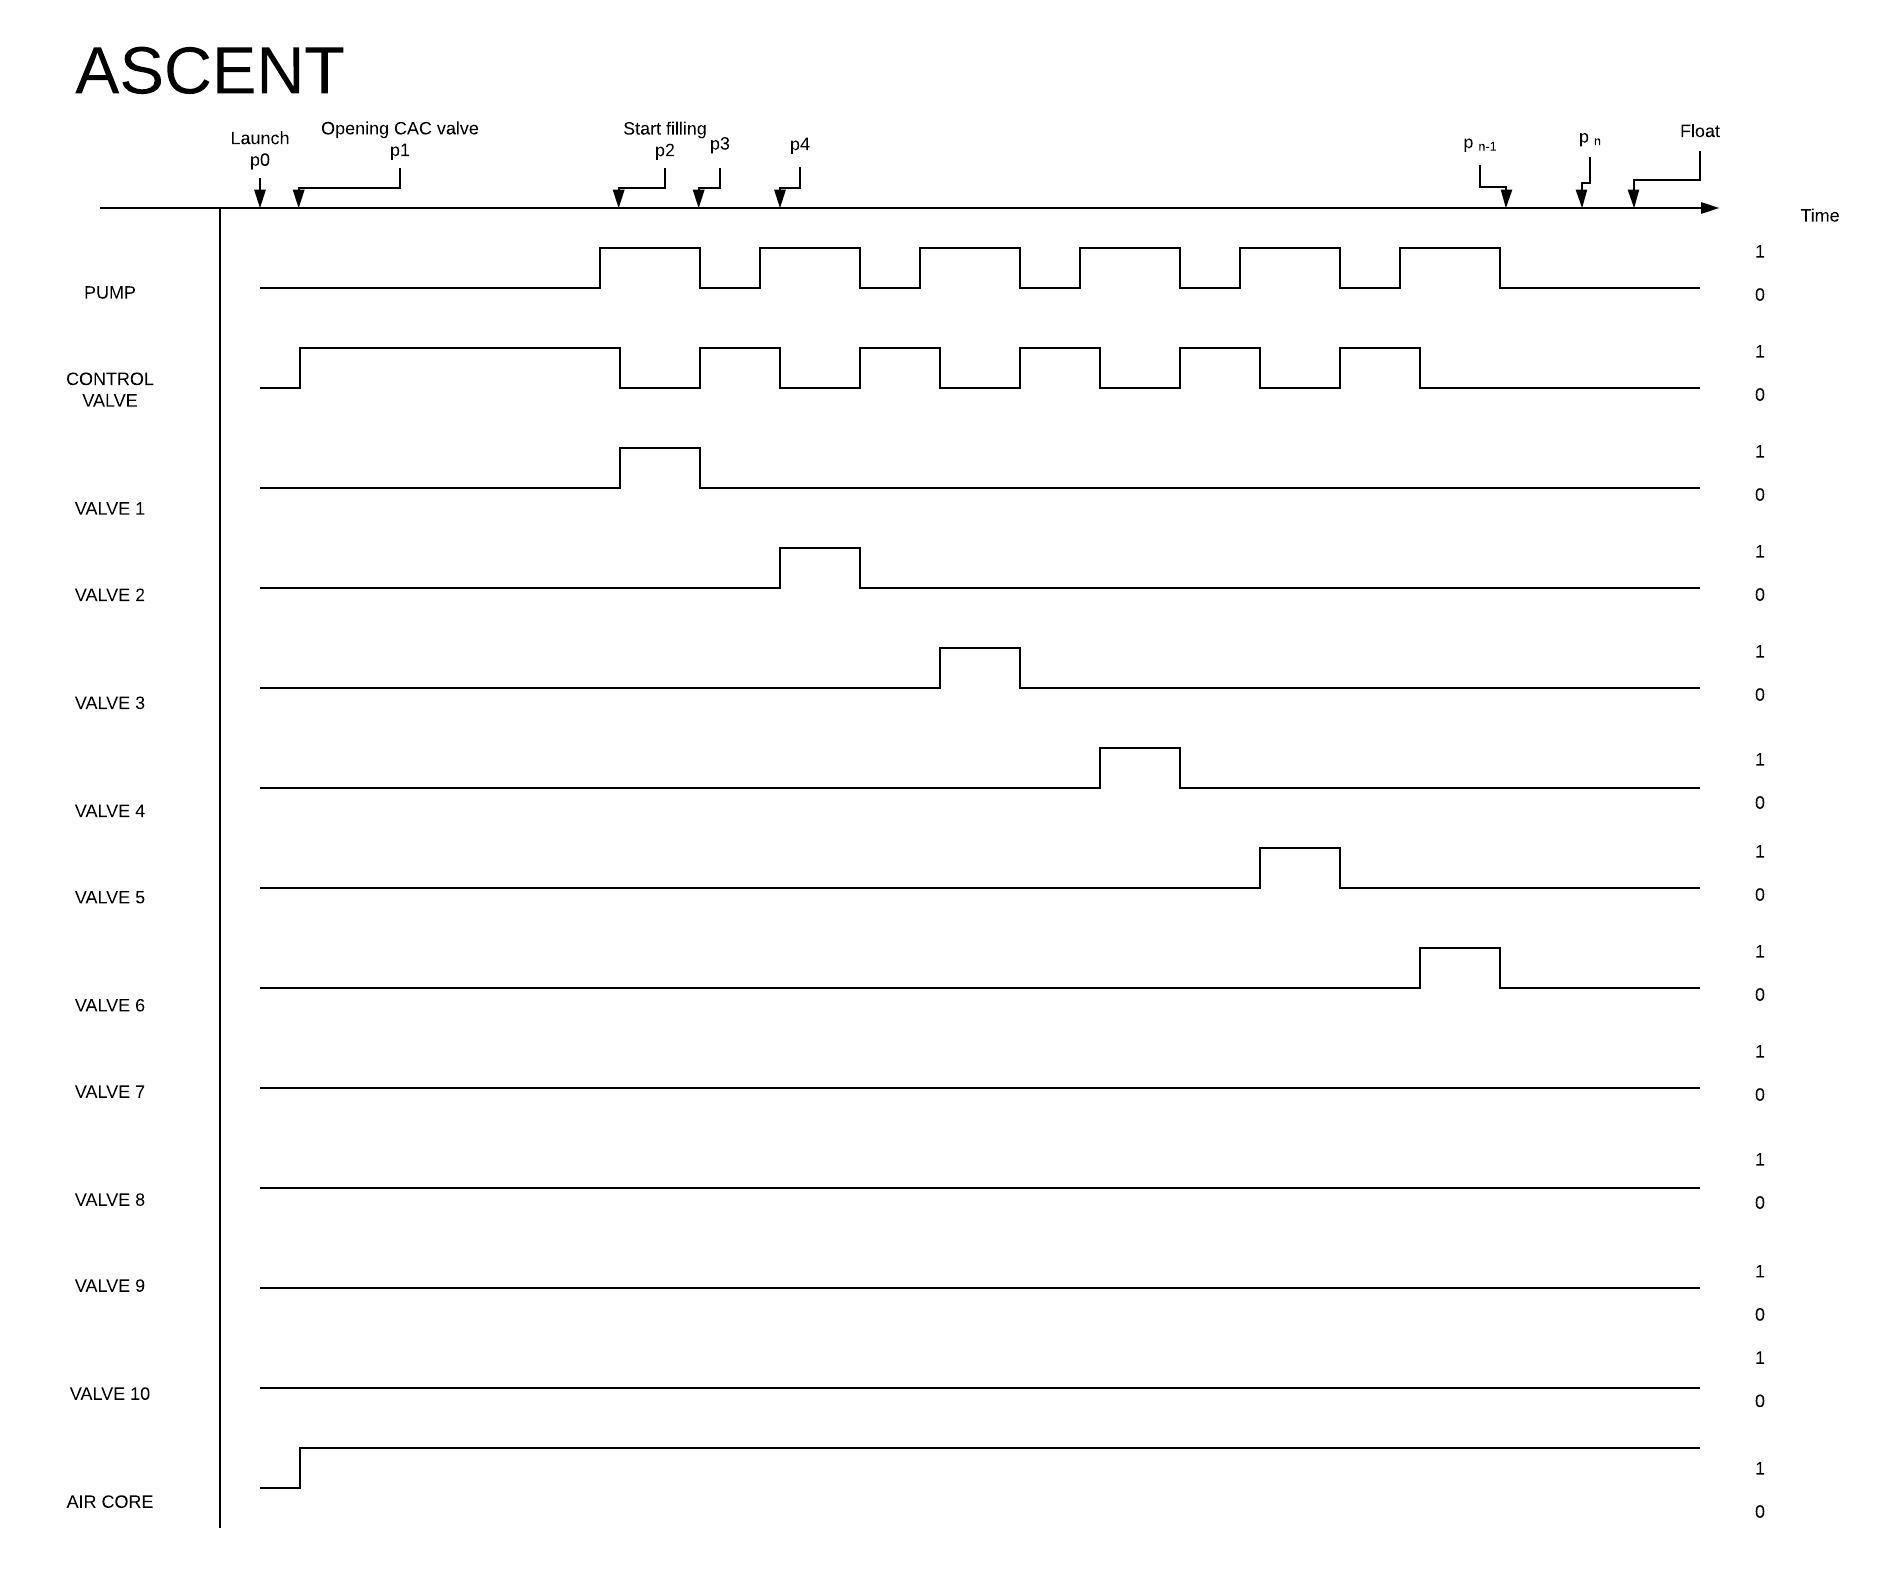
\includegraphics[width=1\linewidth]{4-experiment-design/img/ascent-phase.jpeg}
    \end{align*}
    \caption{The \DIFdelbeginFL \DIFdelFL{emptying }\DIFdelendFL \DIFaddbeginFL \DIFaddFL{Emptying }\DIFaddendFL and \DIFdelbeginFL \DIFdelFL{sampling sequence-Ascent }\DIFdelendFL \DIFaddbeginFL \DIFaddFL{Sampling Sequence-Ascent }\DIFaddendFL Phase\label{fig:ascent}}
\end{figure}

\begin{figure}[H]
    \begin{align*}
        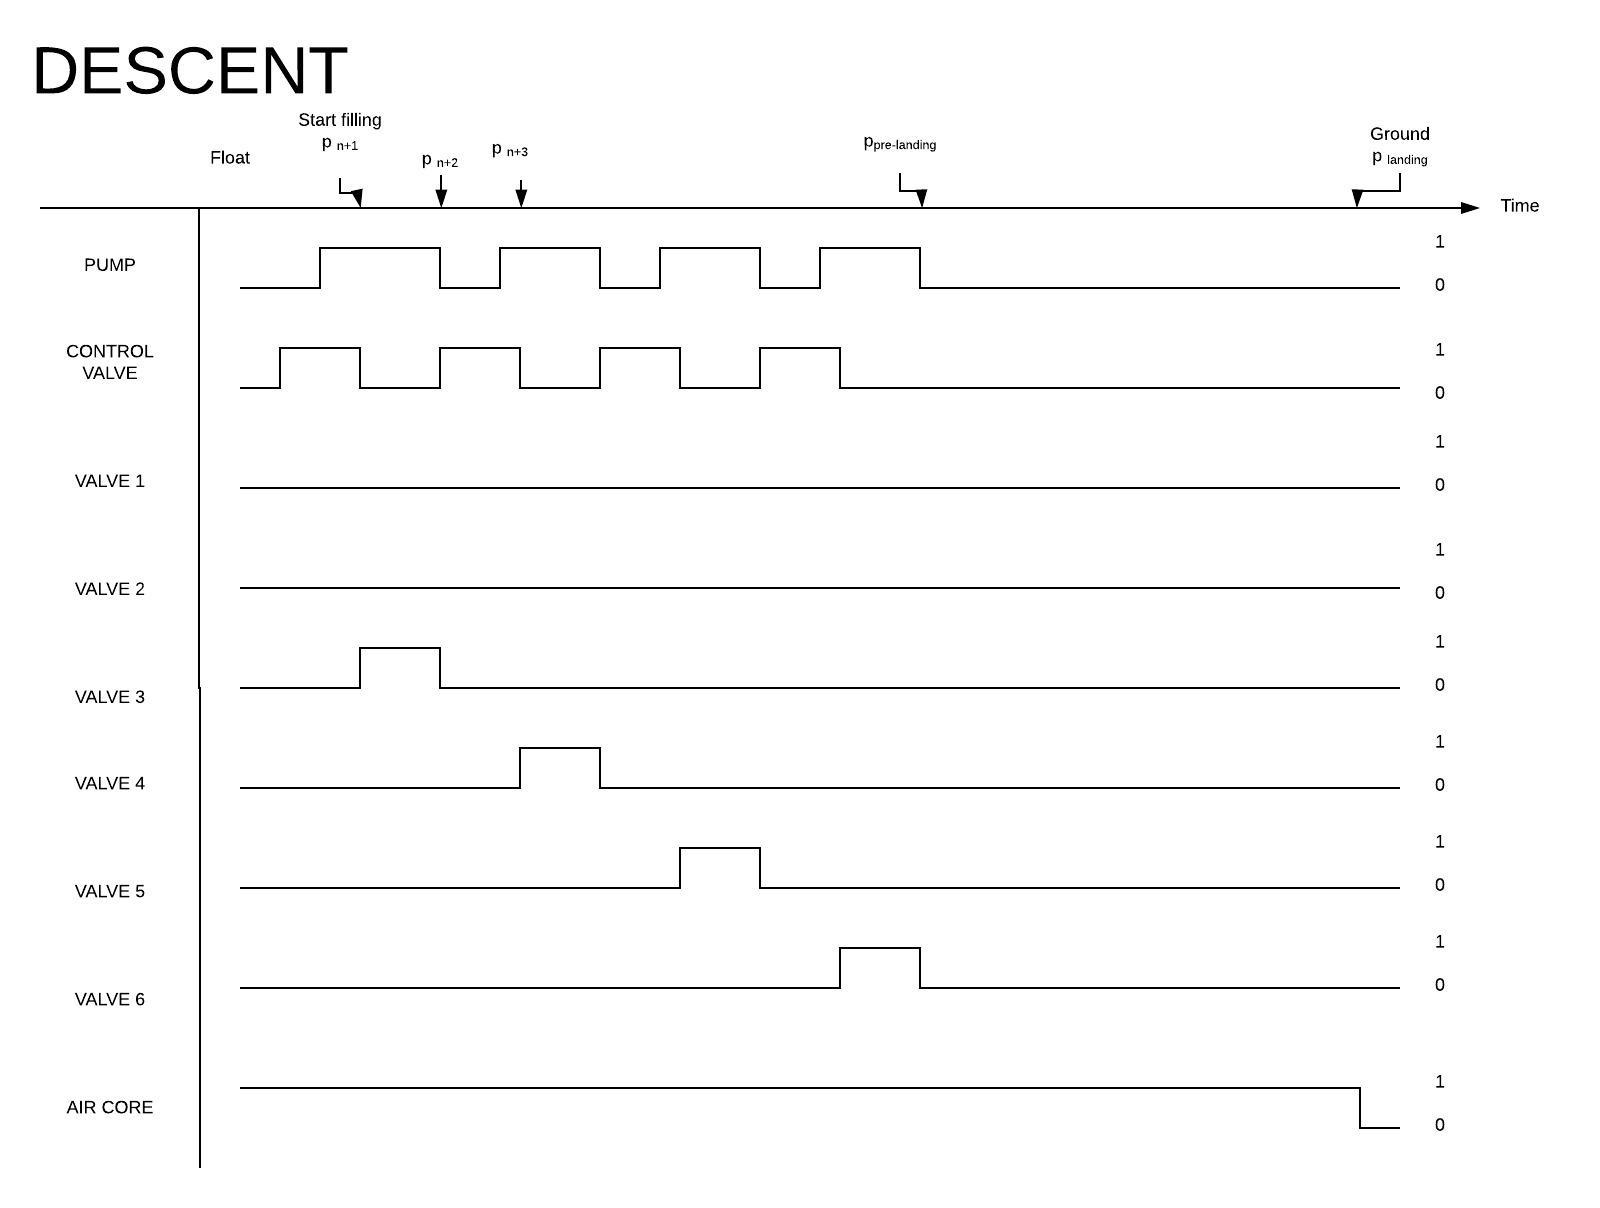
\includegraphics[width=1\linewidth]{4-experiment-design/img/descent-phase.jpeg}
    \end{align*}
    \caption{The \DIFdelbeginFL \DIFdelFL{emptying }\DIFdelendFL \DIFaddbeginFL \DIFaddFL{Emptying }\DIFaddendFL and \DIFdelbeginFL \DIFdelFL{sampling sequence-Descent }\DIFdelendFL \DIFaddbeginFL \DIFaddFL{Sampling Sequence-Descent }\DIFaddendFL Phase\label{fig:descent}}
\end{figure}

In the diagrams, 0 denotes closed/off and 1 denotes opened/on. \DIFaddbegin \DIFadd{The horizontal axis denotes the different pressure levels throughout the flight, with p\mbox{%DIFAUXCMD
$_0$
}%DIFAUXCMD
being the sea level pressure and p\mbox{%DIFAUXCMD
$_8$
}%DIFAUXCMD
being the pressure during Float Phase.
}\DIFaddend 

The \DIFdelbegin \DIFdel{general }\DIFdelend \DIFaddbegin \DIFadd{ambient pressure dependent }\DIFaddend timeline of the experiment is as follow:

\textbf{Ascent Phase:}\\
$p_0$ – $p_1$
\begin{itemize}
    \item CAC valve shall be closed.
    \item AAC valves shall be closed.
    \DIFdelbegin %DIFDELCMD < \item %%%
\item%DIFAUXCMD
\DIFdel{AAC' control valve shall be closed.
    }\DIFdelend \end{itemize}
$p_1$ – $p_2$
\begin{itemize}
    \item CAC valve shall be opened.
    \item \DIFdelbegin \DIFdel{AAC valves shall be closed.
    }%DIFDELCMD < \item %%%
\item%DIFAUXCMD
\DIFdelend CAC tube shall \DIFdelbegin \DIFdel{be flushed.
    }\DIFdelend \DIFaddbegin \DIFadd{start flushing.
    }\end{itemize}

\DIFadd{\mbox{%DIFAUXCMD
$p_2$
}%DIFAUXCMD
– \mbox{%DIFAUXCMD
$p_3$
}%DIFAUXCMD
}\begin{itemize}
    \DIFaddend \item AAC \DIFdelbegin \DIFdel{' control }\DIFdelend \DIFaddbegin \DIFadd{flushing }\DIFaddend valve shall be \DIFaddbegin \DIFadd{opened, allowing for the system to flush.
    }\item \DIFadd{CAC valve remains }\DIFaddend open.
    \end{itemize}
\DIFdelbegin \DIFdel{\mbox{%DIFAUXCMD
$p_2$
}%DIFAUXCMD
– }\DIFdelend $p_3$ \DIFaddbegin \DIFadd{– \mbox{%DIFAUXCMD
$p_4$
}%DIFAUXCMD
}\DIFaddend \begin{itemize}
    \item \DIFdelbegin \DIFdel{Sampling bags' control }\DIFdelend \DIFaddbegin \DIFadd{AAC flushing }\DIFaddend valve shall be closed.
    \item \DIFdelbegin \DIFdel{Sampling bag valve }\DIFdelend \DIFaddbegin \DIFadd{Valve }\DIFaddend 1 shall be opened, allowing for air to enter the first bag.
    \item CAC valve remains open.
    \end{itemize}
\DIFdelbegin \DIFdel{\mbox{%DIFAUXCMD
$p_3$
}%DIFAUXCMD
– }\DIFdelend $p_4$ \DIFaddbegin \DIFadd{– \mbox{%DIFAUXCMD
$p_5$
}%DIFAUXCMD
}\DIFaddend \begin{itemize}
    \item \DIFdelbegin \DIFdel{Sampling bag valve }\DIFdelend \DIFaddbegin \DIFadd{Valve }\DIFaddend 1 shall be closed\DIFaddbegin \DIFadd{.
    }\DIFaddend \item \DIFdelbegin \DIFdel{Sampling bags' control }\DIFdelend \DIFaddbegin \DIFadd{AAC flushing }\DIFaddend valve shall be \DIFaddbegin \DIFadd{closed.
    }\item \DIFadd{CAC valve remains open.
    }\end{itemize}
\DIFadd{\mbox{%DIFAUXCMD
$p_5$
}%DIFAUXCMD
- \mbox{%DIFAUXCMD
$p_6$
}%DIFAUXCMD
}\begin{itemize}
    \item \DIFadd{AAC flushing valve shall be }\DIFaddend opened, allowing the system to flush. 
    \DIFaddbegin \item \DIFadd{CAC valve remains open.
    }\DIFaddend \end{itemize}
\DIFdelbegin \DIFdel{\mbox{%DIFAUXCMD
$p_4$
}%DIFAUXCMD
}\DIFdelend \DIFaddbegin \DIFadd{\mbox{%DIFAUXCMD
$p_6$
}%DIFAUXCMD
}\DIFaddend - \DIFdelbegin \DIFdel{\mbox{%DIFAUXCMD
$p_{n-1}$
}%DIFAUXCMD
}\DIFdelend \DIFaddbegin \DIFadd{\mbox{%DIFAUXCMD
$p_7$
}%DIFAUXCMD
}\DIFaddend \begin{itemize}
    \item \DIFdelbegin \DIFdel{The above procedures shall repeat itself until the remaining five bags have collected air samples for their assigned altitudes.
    }\DIFdelend \DIFaddbegin \DIFadd{AAC flushing valve shall be closed.
    }\item \DIFadd{Valve 2 shall be opened, allowing for air to enter the second bag.
    }\item \DIFadd{CAC valve remains open.
    }\DIFaddend \end{itemize}
\DIFdelbegin \DIFdel{\mbox{%DIFAUXCMD
$p_{n-1}$
}%DIFAUXCMD
– \mbox{%DIFAUXCMD
$p_n$
}%DIFAUXCMD
}\DIFdelend \DIFaddbegin \DIFadd{\mbox{%DIFAUXCMD
$p_7$
}%DIFAUXCMD
- \mbox{%DIFAUXCMD
$p_8$
}%DIFAUXCMD
}\DIFaddend \begin{itemize}
    \item \DIFdelbegin \DIFdel{Sampling bag valve 6 }\DIFdelend \DIFaddbegin \DIFadd{Valve 2 }\DIFaddend shall be closed.
    \item \DIFdelbegin \DIFdel{Sampling bags' control }\DIFdelend \DIFaddbegin \DIFadd{AAC flushing }\DIFaddend valve shall be closed.
    \DIFaddbegin \item \DIFadd{CAC shall finish flushing.
    }\DIFaddend \end{itemize}    




\textbf{\\Float Phase:}\\
No action \DIFaddbegin \DIFadd{is }\DIFaddend taken other than continued telemetry.
 \DIFdelbegin \DIFdel{Air pump is off.}%DIFDELCMD < \\
%DIFDELCMD <  %%%
\DIFdelend 

\textbf{Descent Phase:}

\DIFdelbegin \DIFdel{Note: Before samplingstarts again, the system has to be flushed.
    }\DIFdelend \DIFaddbegin \DIFadd{\mbox{%DIFAUXCMD
$p_9$
}%DIFAUXCMD
– \mbox{%DIFAUXCMD
$p_{10}$
}%DIFAUXCMD
}\begin{itemize}
    \item \DIFadd{CAC shall start sampling. 
    }\item \DIFadd{AAC valves shall be closed.
}\end{itemize}
\DIFaddend 

\DIFdelbegin \DIFdel{\mbox{%DIFAUXCMD
$p_{n+1}$
}%DIFAUXCMD
}\DIFdelend \DIFaddbegin \DIFadd{\mbox{%DIFAUXCMD
$p_{10}$
}%DIFAUXCMD
}\DIFaddend – \DIFdelbegin \DIFdel{\mbox{%DIFAUXCMD
$p_{n+2}$
}%DIFAUXCMD
}\DIFdelend \DIFaddbegin \DIFadd{\mbox{%DIFAUXCMD
$p_{11}$
}%DIFAUXCMD
}\DIFaddend \begin{itemize}
    \item \DIFdelbegin \DIFdel{Sampling bags' control }\DIFdelend \DIFaddbegin \DIFadd{AAC flushing valve shall be opened allowing the system to flush.
    }\item \DIFadd{CAC valve remains open. 
}\end{itemize}

  
\DIFadd{\mbox{%DIFAUXCMD
$p_{11}$
}%DIFAUXCMD
– \mbox{%DIFAUXCMD
$p_{12}$
}%DIFAUXCMD
}\begin{itemize}
    \item \DIFadd{AAC flushing }\DIFaddend valve shall be closed.
    \item \DIFdelbegin \DIFdel{Sampling bagvalve 7 shall be opened}\DIFdelend \DIFaddbegin \DIFadd{Valve 3 shall be opened, allowing for air to enter the third bag.
    }\item \DIFadd{CAC valve remains open. 
}\end{itemize}

\DIFadd{\mbox{%DIFAUXCMD
$p_{12}$
}%DIFAUXCMD
– \mbox{%DIFAUXCMD
$p_{13}$
}%DIFAUXCMD
}\begin{itemize}
    \item \DIFadd{Valve 3 shall be closed.
    }\item \DIFadd{AAC flushing valve shall be closed.
    }\item \DIFadd{CAC valve remains open.
}\end{itemize}

\DIFadd{\mbox{%DIFAUXCMD
$p_{13}$
}%DIFAUXCMD
– \mbox{%DIFAUXCMD
$p_{14}$
}%DIFAUXCMD
}\begin{itemize}
    \item \DIFadd{AAC flushing valve shall be opened allowing the system to flush.
    }\item \DIFadd{CAC valve remains open.
}\end{itemize}

\DIFadd{\mbox{%DIFAUXCMD
$p_{14}$
}%DIFAUXCMD
– \mbox{%DIFAUXCMD
$p_{15}$
}%DIFAUXCMD
}\begin{itemize}
    \item \DIFadd{AAC flushing valve shall be closed.
    }\item \DIFadd{Valve 4 shall be opened}\DIFaddend , allowing for air to enter the \DIFdelbegin \DIFdel{first bag.
    }\DIFdelend \DIFaddbegin \DIFadd{fourth bag.
    }\item \DIFadd{CAC valve remains open.
}\DIFaddend \end{itemize}

\DIFdelbegin \DIFdel{\mbox{%DIFAUXCMD
$p_{n+2}$
}%DIFAUXCMD
}\DIFdelend \DIFaddbegin \DIFadd{\mbox{%DIFAUXCMD
$p_{15}$
}%DIFAUXCMD
}\DIFaddend – \DIFdelbegin \DIFdel{\mbox{%DIFAUXCMD
$p_{n+3}$
}%DIFAUXCMD
}\DIFdelend \DIFaddbegin \DIFadd{\mbox{%DIFAUXCMD
$p_{16}$
}%DIFAUXCMD
}\DIFaddend \begin{itemize}
    \item \DIFdelbegin \DIFdel{Sampling bag valve 7 }\DIFdelend \DIFaddbegin \DIFadd{Valve 4 shall be closed.
    }\item \DIFadd{AAC flushing valve }\DIFaddend shall be closed\DIFaddbegin \DIFadd{.
    }\DIFaddend \item \DIFdelbegin \DIFdel{Sampling bags' control valve }\DIFdelend \DIFaddbegin \DIFadd{CAC valve remains open.
}\end{itemize}

\DIFadd{\mbox{%DIFAUXCMD
$p_{16}$
}%DIFAUXCMD
– \mbox{%DIFAUXCMD
$p_{17}$
}%DIFAUXCMD
}\begin{itemize}
    \item \DIFadd{AAC flushing valve }\DIFaddend shall be opened, allowing the system to flush. 
    \DIFaddbegin \item \DIFadd{CAC remains open.
  }\DIFaddend \end{itemize}

\DIFdelbegin \DIFdel{In between, same procedure shall repeat itself until all the remaining bags have collected air samples for their assigned altitudes.
}\DIFdelend \DIFaddbegin \DIFadd{\mbox{%DIFAUXCMD
$p_{17}$
}%DIFAUXCMD
– \mbox{%DIFAUXCMD
$p_{18}$
}%DIFAUXCMD
}\begin{itemize}
    \item \DIFadd{AAC flushing valve shall be closed.
    }\item \DIFadd{Valve 5 shall be opened, allowing for air to enter the fifth bag. 
    }\item \DIFadd{CAC valve remains open.
}\end{itemize}
\DIFaddend 

\DIFaddbegin \DIFadd{\mbox{%DIFAUXCMD
$p_{18}$
}%DIFAUXCMD
– \mbox{%DIFAUXCMD
$p_{19}$
}%DIFAUXCMD
}\begin{itemize}
    \item \DIFadd{Valve 5 shall be closed.
    }\item \DIFadd{AAC flushing valve shall be closed.
    }\item \DIFadd{CAC valve remains open.
}\end{itemize}

\DIFadd{\mbox{%DIFAUXCMD
$p_{19}$
}%DIFAUXCMD
– \mbox{%DIFAUXCMD
$p_{20}$
}%DIFAUXCMD
}\begin{itemize}
     \item \DIFadd{AAC flushing valve shall be opened, allowing the system to flush. 
    }\item \DIFadd{CAC remains open.
   }\end{itemize}

\DIFadd{\mbox{%DIFAUXCMD
$p_{20}$
}%DIFAUXCMD
– \mbox{%DIFAUXCMD
$p_{21}$
}%DIFAUXCMD
}\begin{itemize}
    \item \DIFadd{AAC flushing valve shall be closed.
    }\item \DIFadd{Valve 6 shall be opened, allowing for air to enter the sixth bag.
}\end{itemize}

\DIFaddend $p_{pre-landing}$ 
\begin{itemize}
    \item \DIFdelbegin \DIFdel{System Sampling bag valve 10 }\DIFdelend \DIFaddbegin \DIFadd{Valve 6 }\DIFaddend shall be closed.
    \item \DIFdelbegin \DIFdel{Sampling bags' control }\DIFdelend \DIFaddbegin \DIFadd{AAC flushing }\DIFaddend valve shall be closed\DIFaddbegin \DIFadd{.
    }\DIFaddend \item CAC valve shall be opened.
\end{itemize}

\DIFdelbegin \DIFdel{\mbox{%DIFAUXCMD
$p_{landing}$
}%DIFAUXCMD
}\DIFdelend \DIFaddbegin \DIFadd{\mbox{%DIFAUXCMD
$p_{0-landing}$
}%DIFAUXCMD
}\DIFaddend \begin{itemize}
    \item CAC valve shall be closed.
\end{itemize}


Note: The AAC system's air pump is only on during sampling into the air sampling bags and flushing of the system.


\raggedbottom
\pagebreak
\subsection{Experiment Interfaces}

\subsubsection{Mechanical Interfaces}
\DIFaddbegin \label{sec:4.2.1}
\DIFaddend The experiment box will be fixed to the gondola rails by means of \DIFdelbegin \DIFdel{4 screws }\DIFdelend \DIFaddbegin \DIFadd{eight brackets, as seen in Figure \ref{fig:bracket}, }\DIFaddend interfacing the experiment outside structure with the hammer nuts in the rails. \DIFdelbegin \DIFdel{90-degree aluminum angles will be used to provide this interface.}\DIFdelend This method is secure as well as fast enough to provide an accessible and easy \DIFdelbegin \DIFdel{recuperation for the }\DIFdelend \DIFaddbegin \DIFadd{recovery for }\DIFaddend later analysis.

\DIFdelbegin \DIFdel{Lateral and top }\DIFdelend \DIFaddbegin \begin{figure}[H]
    \centering
    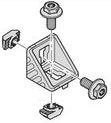
\includegraphics[width=0.2\textwidth]{4-experiment-design/img/Mechanical/bracket.jpg}
    \caption{\DIFaddFL{Bracket Component}}
    \label{fig:bracket}
\end{figure}

\DIFadd{A simple but reliable fixing interface between the two boxes of the experiment has been designed to ensure the fast recovery of the CAC box. The latter implies only unscrewing 12 bolts as well as unplugging a D-Sub connector. Once the CAC box is detached, the AAC Box will still remain perfectly fixed in the gondola. Table \ref{table:attaching-components} gathers up all the components required to fix the experiment to the gondola. 
}

\begin{table}[H]
\noindent\DIFaddFL{\makebox[\columnwidth]{%
\scalebox{0.8}{
\begin{tabular}{|c|c|c|c|c|c|}
\hline
Component & Interface & Amount & Dimensions & Weight/unit & Total weight \\ \hline
Bracket standard 20/20 slot 6/6 & AAC-Gondola & \mbox{%DIFAUXCMD
$8$
}%DIFAUXCMD
& \mbox{%DIFAUXCMD
$20x20x20\ mm$
}%DIFAUXCMD
& \mbox{%DIFAUXCMD
$5g$
}%DIFAUXCMD
& \mbox{%DIFAUXCMD
$40g$
}%DIFAUXCMD
\\ \hline
6-hole plate & AAC-CAC & \mbox{%DIFAUXCMD
$4$
}%DIFAUXCMD
& \mbox{%DIFAUXCMD
$1x60x40\ mm$
}%DIFAUXCMD
& \mbox{%DIFAUXCMD
$50g$
}%DIFAUXCMD
& \mbox{%DIFAUXCMD
$200g$
}%DIFAUXCMD
\\ \hline
T-nut slot 6 M4 & AAC-CAC, AAC-Gondola & \mbox{%DIFAUXCMD
$40$
}%DIFAUXCMD
& \mbox{%DIFAUXCMD
$4x5.9x11.5\ mm$
}%DIFAUXCMD
& \mbox{%DIFAUXCMD
$3g$
}%DIFAUXCMD
& \mbox{%DIFAUXCMD
$120g$
}%DIFAUXCMD
\\ \hline
bolt M4 & AAC-CAC, AAC-Gondola & \mbox{%DIFAUXCMD
$40$
}%DIFAUXCMD
& \mbox{%DIFAUXCMD
$8 mm $
}%DIFAUXCMD
length & \mbox{%DIFAUXCMD
$1g$
}%DIFAUXCMD
& \mbox{%DIFAUXCMD
$40g$
}%DIFAUXCMD
\\ \hline
washer M4 & AAC-CAC, AAC-Gondola & \mbox{%DIFAUXCMD
$24$
}%DIFAUXCMD
& \mbox{%DIFAUXCMD
$ID=4.3mm$
}%DIFAUXCMD
, \mbox{%DIFAUXCMD
$OD=9mm$
}%DIFAUXCMD
& \mbox{%DIFAUXCMD
$0.2g$
}%DIFAUXCMD
& \mbox{%DIFAUXCMD
$4.8g$
}%DIFAUXCMD
\\ \hline
\end{tabular}}}
}\caption{\DIFaddFL{Gondola-AAC and AAC-CAC Interfaces Attaching Components}}
\label{table:attaching-components}
\end{table}


\DIFadd{Top }\DIFaddend handles will be mounted to facilitate the experiment box manipulation when moving it in and out of the gondola. 
\DIFdelbegin %DIFDELCMD < 

%DIFDELCMD < %%%
\DIFdelend In order to collect reliable air samples, the experiment requires to be mounted at least with one side exposed to the outside. The later will reduce the pipe length used to collect clean air. Three tubes will extend from the experiment box face\DIFdelbegin \DIFdel{, see Figure \ref{fig:pipes_interface}}\DIFdelend . One for the CAC sampling and two, input and output, for the AAC sampling. The one-way selected method will provide a proper flushing of the pipe and thus ensure a reliable sampling as explained in \DIFdelbegin \DIFdel{section }\DIFdelend \DIFaddbegin \DIFadd{Section }\DIFaddend \ref{Experiment_Setup}.


\DIFdelbegin %DIFDELCMD < \begin{figure}[H]
%DIFDELCMD <     %%%
\begin{align*}
        \DIFdelFL{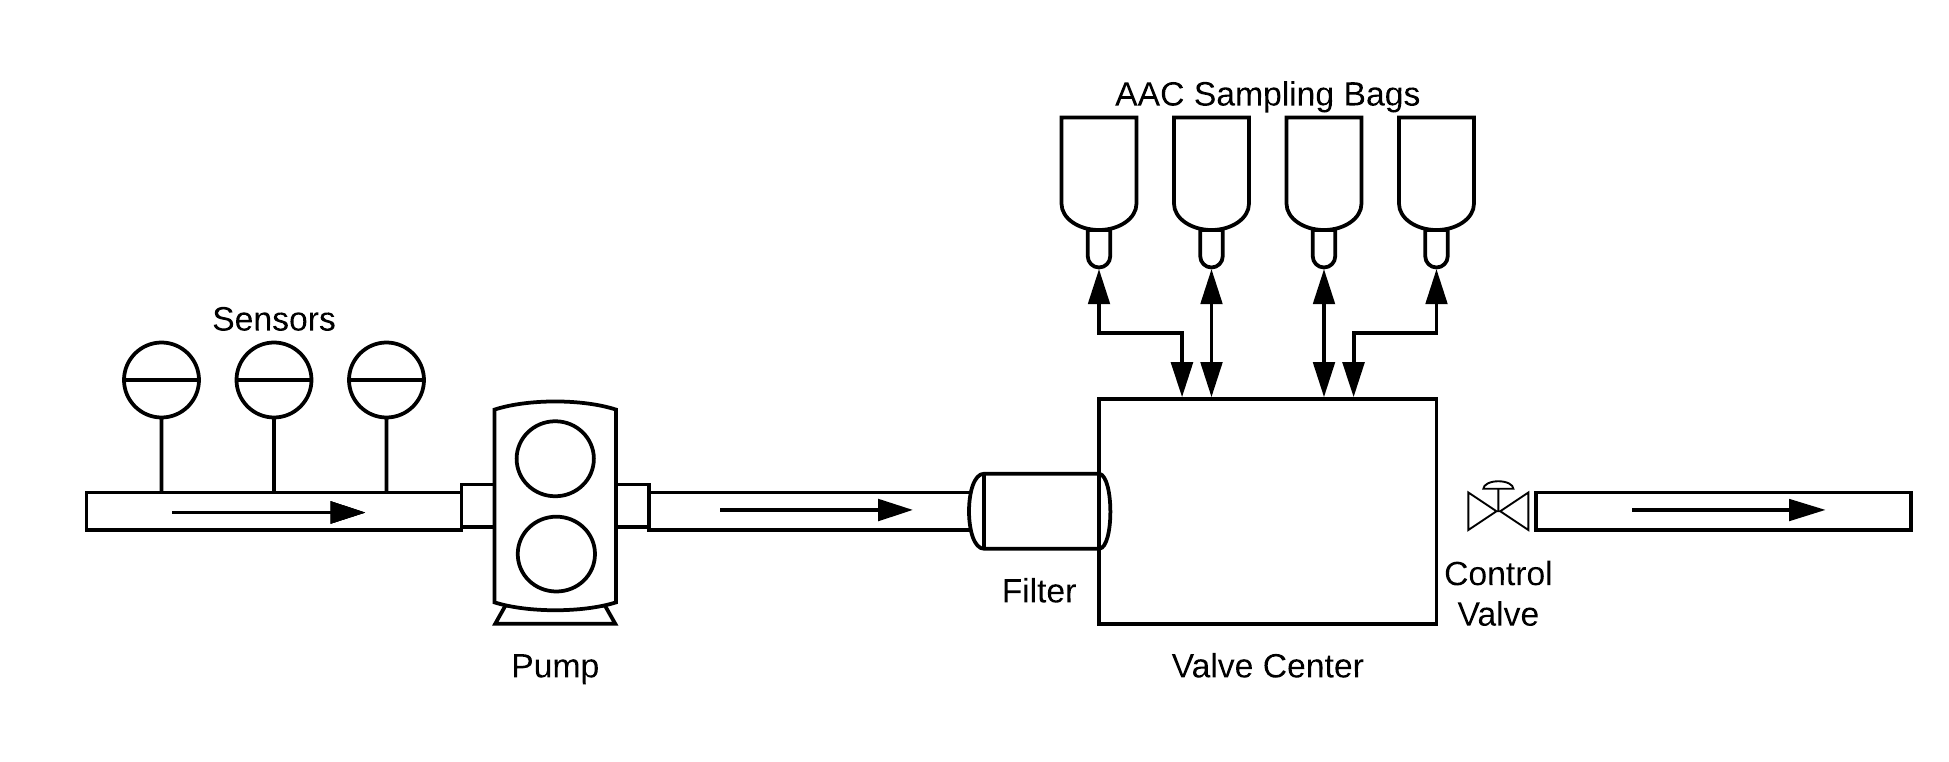
\includegraphics[width=0.7\textwidth]{4-experiment-design/img/Schematic_pipe.png}
    }\end{align*}
    %DIFAUXCMD
%DIFDELCMD < \caption{%
{%DIFAUXCMD
\DIFdelFL{Schematic of air sampler pipe.}}%DIFAUXCMD
%DIFDELCMD < \label{fig:pipes_interface}
%DIFDELCMD < \end{figure}
%DIFDELCMD < 

%DIFDELCMD < \bigskip
%DIFDELCMD < 

%DIFDELCMD < %%%
\DIFdelend \DIFaddbegin \pagebreak
\DIFaddend \subsubsection{Electrical Interfaces}
\DIFdelbegin %DIFDELCMD < \begin{centering}
%DIFDELCMD < %%%
\DIFdelend \DIFaddbegin \label{sec:4.2.2}

\DIFaddend The experiment will connect to the gondola electrically via a 4 pin, male, box mount receptacle MIL - C-26482P series 1 connector with an 8-4 insert arrangement (MS3112E8-4P) \cite{BexusManual}. It will connect to one 28.8 V/\DIFdelbegin \DIFdel{1mA }\DIFdelend \DIFaddbegin \DIFadd{1 mA }\DIFaddend battery pack which consists of eight SAFT LSH20 batteries in series where each has a \DIFdelbegin \DIFdel{5A }\DIFdelend \DIFaddbegin \DIFadd{5 A }\DIFaddend fuse\cite{BexusManual}. The expected maximum current is \DIFdelbegin \DIFdel{1.33A.
}%DIFDELCMD < \end{centering}
%DIFDELCMD < \bigskip
%DIFDELCMD < %%%
\DIFdelend \DIFaddbegin \DIFadd{1.1 A.
}\DIFaddend 

\DIFdelbegin %DIFDELCMD < \begin{centering}
%DIFDELCMD < %%%
\DIFdelend \DIFaddbegin \begin{figure}[H]
    \centering
    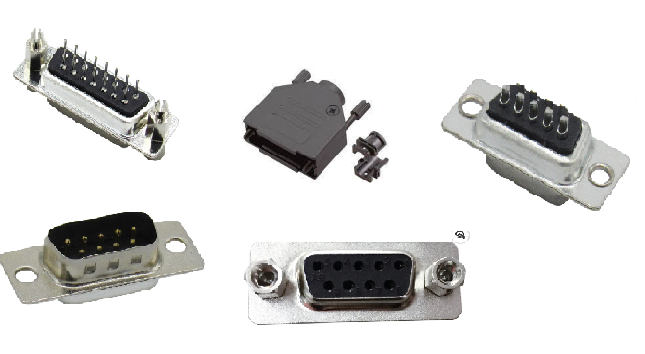
\includegraphics[width=0.4\textwidth]{4-experiment-design/img/connectors.png}
    \caption{\DIFaddFL{Connectors}}
    \label{fig:connectors}
\end{figure}

\DIFaddend The E-Link connection shall be made between the experiment and the E-Link system using a RJ45 connection which will be supplied by SSC and an Ethernet protocol. The Amphenol RJF21B connector will be mounted on either the front or the side of the experiment\cite{BexusManual}.  
\DIFdelbegin %DIFDELCMD < \end{centering}
%DIFDELCMD < \bigskip
%DIFDELCMD < %%%
\DIFdelend 

\DIFdelbegin %DIFDELCMD < \begin{centering}
%DIFDELCMD < %%%
\DIFdel{The }\DIFdelend \DIFaddbegin \DIFadd{The CAC and AAC will be connected together with a D-SUB 9-pin connector where power, ground and signals for the sensors in the CAC will be connected. A female connector will be located on the AAC wall and a male connector on the CAC wall.
}

\DIFadd{Another female D-SUB 9-pin connector will be located on the wall of the AAC in which the connections for the three ambient pressure sensors will be located. Connectors with different pin configuration are shown in Figure \ref{fig:connectors}.
}

\DIFadd{The }\DIFaddend expected data rate is \DIFdelbegin \DIFdel{2kbit}\DIFdelend \DIFaddbegin \DIFadd{1.58 kbits}\DIFaddend /s \DIFdelbegin \DIFdel{with 10kbit}\DIFdelend \DIFaddbegin \DIFadd{for downlink and 1.08 kbits}\DIFaddend /\DIFdelbegin \DIFdel{s peak downlink and 5kbit/}\DIFdelend s \DIFdelbegin \DIFdel{peak uplink.
}%DIFDELCMD < \end{centering}
%DIFDELCMD < %%%
\DIFdelend \DIFaddbegin \DIFadd{for uplink.
}\DIFaddend 

%\begin{figure}[H]
%    \begin{align*}
%        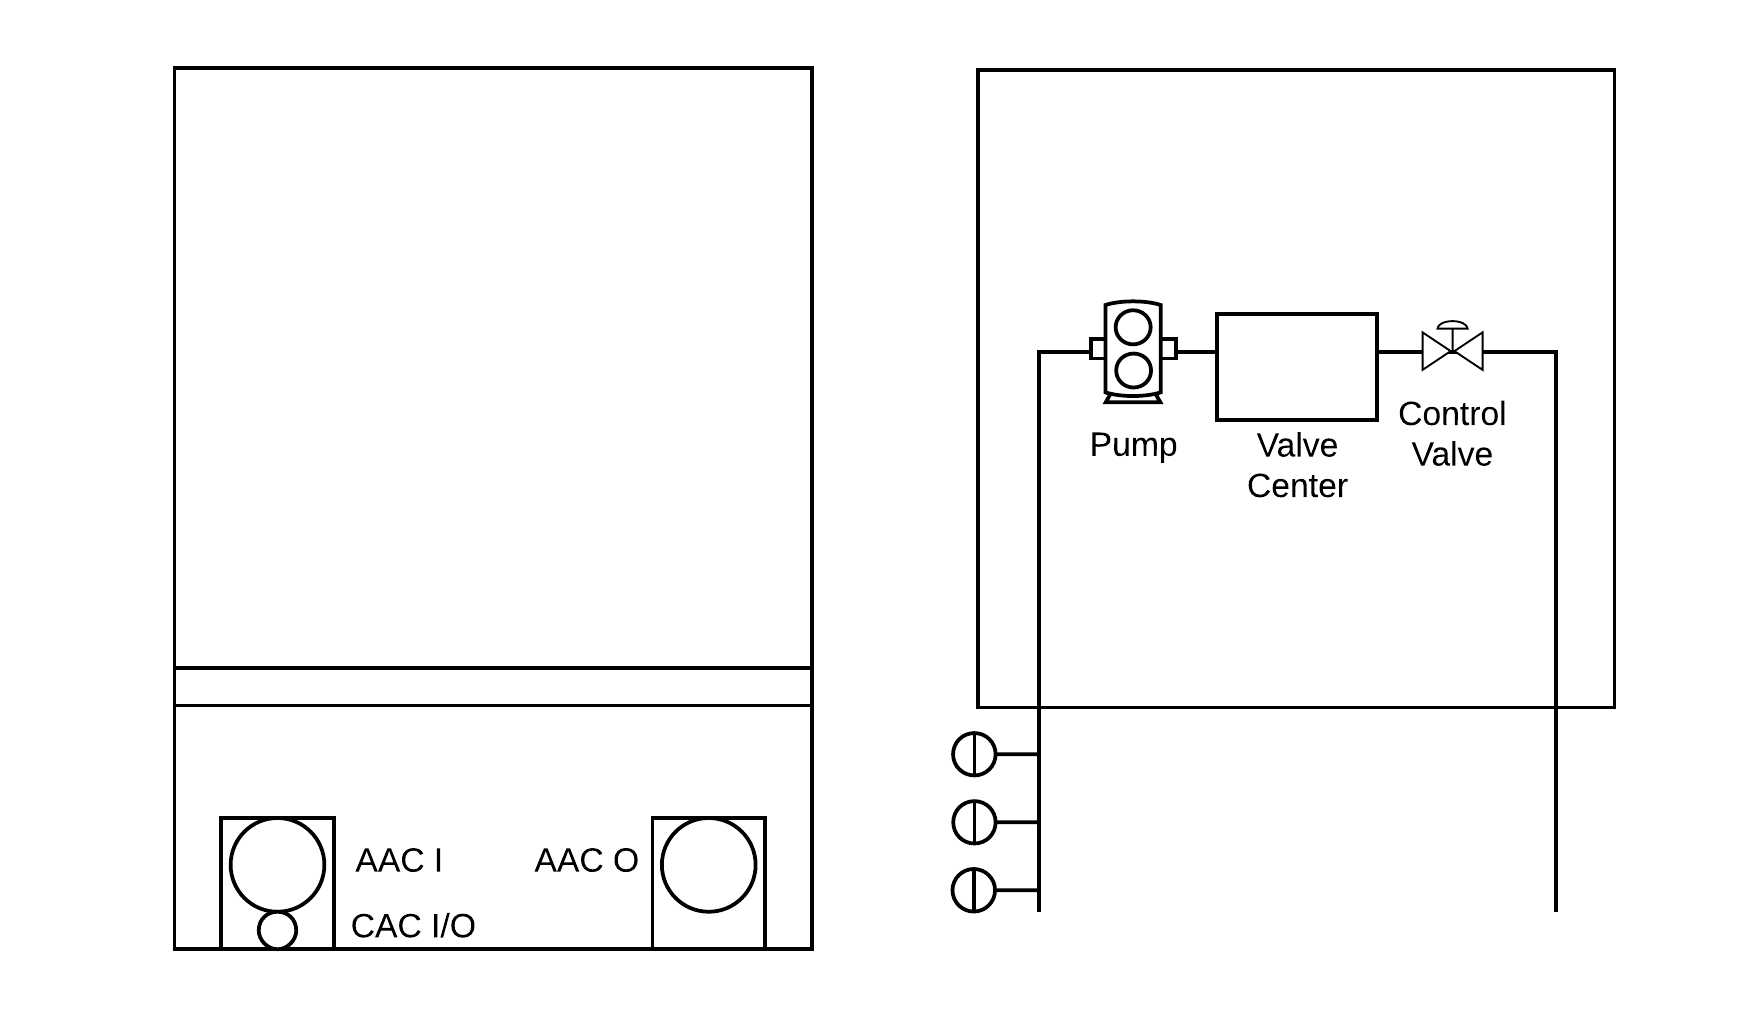
\includegraphics[width=0.7\textwidth]{4-experiment-design/img/Diagram_pipe.png}
%    \end{align*}
%    \caption{Diagram of the experiment box face exposed to the outside.}\label{fig:pipes_interface_1}
%\end{figure}

\iffalse
\subsubsection{Radio Frequencies (Optional)}
\begin{centering}
Not required.
\end{centering}
\bigskip

\subsubsection{Thermal (Optional)}
\begin{centering}
Not required.
\end{centering}
\bigskip
\fi


\raggedbottom
\begin{landscape}
\subsection{Experiment Components} \DIFaddbegin \label{components}
\label{sec:experiment-components}

\DIFadd{Component tables were generated from the project budget spreadsheet in Appendix \ref{sec:appO} using the scripts included in Appendix \ref{sec:appK}. Table headers are letter coded and correspond to the following:
}

\textbf{\DIFadd{A}} \DIFadd{- Components Name}\\
\textbf{\DIFadd{B}} \DIFadd{- Manufacturer}\\
\textbf{\DIFadd{C}} \DIFadd{- Manufacturer Code}\\
\textbf{\DIFadd{D}} \DIFadd{- Quantity}\\
\textbf{\DIFadd{E}} \DIFadd{- Total Cost }[\DIFadd{EUR}]\\
\textbf{\DIFadd{F}} \DIFadd{- Total Mass }[\DIFadd{g}]\\
\textbf{\DIFadd{G}} \DIFadd{- Note}\\
\textbf{\DIFadd{H}} \DIFadd{- Status}\\

\DIFaddend \subsubsection{Electrical Components}

Table \DIFdelbegin \DIFdel{\ref{tab:electrical-components} }\DIFdelend \DIFaddbegin \DIFadd{\ref{tab:components-table-electrical} }\DIFaddend shows all required electrical components with \DIFaddbegin \DIFadd{their total }\DIFaddend mass and price.\DIFaddbegin \\
\DIFaddend 

\DIFdelbegin %DIFDELCMD < \begin{longtable}{|m{0.03\textwidth}|m{0.3\textwidth}|m{0.25\textwidth}|m{0.05\textwidth}|m{0.1\textwidth}|m{0.3\textwidth}|m{0.15\textwidth}|m{0.08\textwidth}|}
%DIFDELCMD <     

%DIFDELCMD < %%%
\DIFdelend \DIFaddbegin \begin{longtable} {\DIFadd{|m}{\DIFadd{0.05\textwidth}}\DIFadd{|m}{\DIFadd{0.25\textwidth}}\DIFadd{|m}{\DIFadd{0.15\textwidth}}\DIFadd{|m}{\DIFadd{0.2\textwidth}}\DIFadd{|m}{\DIFadd{0.05\textwidth}}\DIFadd{|m}{\DIFadd{0.05\textwidth}}\DIFadd{|m}{\DIFadd{0.05\textwidth}}\DIFadd{|m}{\DIFadd{0.25\textwidth}}\DIFadd{|m}{\DIFadd{0.095\textwidth}}\DIFadd{|}} \DIFaddend \hline \textbf{ID} & \textbf{\DIFdelbegin \DIFdel{Components}\DIFdelend \DIFaddbegin \DIFadd{A}\DIFaddend } & \textbf{\DIFdelbegin \DIFdel{Specs (size,weight)}\DIFdelend \DIFaddbegin \DIFadd{B}\DIFaddend } & \textbf{\DIFdelbegin \DIFdel{No.}\DIFdelend \DIFaddbegin \DIFadd{C}\DIFaddend } & \textbf{\DIFdelbegin \DIFdel{Cost}\DIFdelend \DIFaddbegin \DIFadd{D}\DIFaddend } & \textbf{\DIFdelbegin \DIFdel{Note}\DIFdelend \DIFaddbegin \DIFadd{E}\DIFaddend } & \textbf{\DIFdelbegin \DIFdel{Availability}\DIFdelend \DIFaddbegin \DIFadd{F}\DIFaddend }  & \textbf{\DIFdelbegin \DIFdel{Status}\DIFdelend \DIFaddbegin \DIFadd{G}\DIFaddend }  \DIFaddbegin & \textbf{\DIFadd{H}} \DIFaddend \\ \hline \DIFdelbegin \DIFdel{1 }\DIFdelend \DIFaddbegin \DIFadd{E1 }\DIFaddend & Arduino Due & \DIFdelbegin \DIFdel{101.52 mm x 53.3 mm, 36 g }\DIFdelend \DIFaddbegin \DIFadd{Arduino }\DIFaddend & \DIFaddbegin \DIFadd{A000062 }& \DIFaddend 1 & \DIFaddbegin \DIFadd{36 }& \DIFaddend 35 \DIFdelbegin \DIFdel{Euro }\DIFdelend & Fast and has many analog, and digital pins & \DIFdelbegin \DIFdel{Easily ordered online }%DIFDELCMD < & %%%
\DIFdel{Ordered }\DIFdelend \DIFaddbegin \DIFadd{Received }\DIFaddend \\ \hline \DIFdelbegin \DIFdel{2 }\DIFdelend \DIFaddbegin \DIFadd{E2 }\DIFaddend & \DIFdelbegin \DIFdel{W5500 }\DIFdelend Ethernet Shield & \DIFdelbegin \DIFdel{36 g }\DIFdelend \DIFaddbegin \DIFadd{SEEED Studio }\DIFaddend & \DIFaddbegin \DIFadd{SKU 103030021 }& \DIFaddend 1 & \DIFdelbegin \DIFdel{28 Euro }\DIFdelend \DIFaddbegin \DIFadd{36 }\DIFaddend & \DIFdelbegin \DIFdel{Easily, connected }\DIFdelend \DIFaddbegin \DIFadd{30 }& \DIFadd{Can be mounted }\DIFaddend on  top  of the board & \DIFdelbegin \DIFdel{Easily ordered online }%DIFDELCMD < & %%%
\DIFdel{Ordered }\DIFdelend \DIFaddbegin \DIFadd{Received }\DIFaddend \\ \hline \DIFdelbegin \DIFdel{3 }\DIFdelend \DIFaddbegin \DIFadd{E3 }\DIFaddend & \DIFdelbegin \DIFdel{KNF }\DIFdelend \DIFaddbegin \DIFadd{Miniature diaphragm air pump }& \DIFadd{KNF }& \DIFadd{NMP }\DIFaddend 850.1.2 \DIFdelbegin \DIFdel{. KNDC B Miniature Diaphragm Pump }\DIFdelend \DIFaddbegin \DIFadd{KNDC-B }\DIFaddend & \DIFdelbegin \DIFdel{30 x 54.3 x 77.5 mm, 430g  }%DIFDELCMD < & %%%
\DIFdelend 1 & \DIFaddbegin \DIFadd{430 }& \DIFaddend 350 \DIFdelbegin \DIFdel{Euro }\DIFdelend &  \DIFdelbegin \DIFdel{Low power, small size }\DIFdelend & \DIFdelbegin \DIFdel{Easily ordered online }%DIFDELCMD < & %%%
\DIFdel{Ordered }\DIFdelend \DIFaddbegin \DIFadd{Received }\DIFaddend \\ \hline \DIFdelbegin \DIFdel{4 }\DIFdelend \DIFaddbegin \DIFadd{E4 }\DIFaddend & \DIFdelbegin \DIFdel{Barometric Pressure Sensor MS5607-02BA03 }\DIFdelend \DIFaddbegin \DIFadd{Pressure sensor }\DIFaddend & \DIFdelbegin \DIFdel{5.0 x 3.0 x 1.0 mm, 1g  }\DIFdelend \DIFaddbegin \DIFadd{SENSOR SOLUTIONS }\DIFaddend & \DIFdelbegin \DIFdel{3 }\DIFdelend \DIFaddbegin \DIFadd{MS560702BA03-50 }\DIFaddend & \DIFdelbegin \DIFdel{11 Euro }\DIFdelend \DIFaddbegin \DIFadd{7 }\DIFaddend & \DIFaddbegin \DIFadd{5 }& \DIFadd{1.9 }& \DIFaddend High  resolution,  large  measuring range & \DIFdelbegin \DIFdel{Easily ordered online }%DIFDELCMD < & %%%
\DIFdel{To be ordered online }\DIFdelend \DIFaddbegin \DIFadd{To Be Ordered }\DIFaddend \\ \hline \DIFdelbegin \DIFdel{5 }\DIFdelend \DIFaddbegin \DIFadd{E5 }\DIFaddend & \DIFdelbegin \DIFdel{Electromagnetically controlled valve }%DIFDELCMD < & %%%
\DIFdel{1-1}\DIFdelend \DIFaddbegin \DIFadd{Sampling Valve (inlet and outlet 1}\DIFaddend /\DIFdelbegin \DIFdel{4}\DIFdelend \DIFaddbegin \DIFadd{8}\DIFaddend " \DIFdelbegin \DIFdel{, 2640 g }\DIFdelend \DIFaddbegin \DIFadd{female) }\DIFaddend & \DIFdelbegin \DIFdel{12 }\DIFdelend \DIFaddbegin \DIFadd{SMC }\DIFaddend & \DIFdelbegin \DIFdel{1756 Euro }\DIFdelend \DIFaddbegin \DIFadd{VDW22UANXB }\DIFaddend & \DIFdelbegin \DIFdel{Cascaded/series of valves }\DIFdelend \DIFaddbegin \DIFadd{1 }\DIFaddend & \DIFdelbegin \DIFdel{Easily ordered online }\DIFdelend \DIFaddbegin \DIFadd{100 }\DIFaddend & \DIFdelbegin \DIFdel{One ordered for testing }\DIFdelend \DIFaddbegin \DIFadd{45 }&  & \DIFadd{To Be Ordered }\DIFaddend \\ \hline \DIFdelbegin \DIFdel{6 }\DIFdelend \DIFaddbegin \DIFadd{E6 }\DIFaddend & Airflow sensor \DIFdelbegin \DIFdel{AWM40000 Series }\DIFdelend & \DIFdelbegin \DIFdel{14 g }\DIFdelend \DIFaddbegin \DIFadd{Honeywell }\DIFaddend & \DIFaddbegin \DIFadd{AWM5102VN }& \DIFaddend 1 & \DIFdelbegin \DIFdel{106 Euro }\DIFdelend \DIFaddbegin \DIFadd{60 }\DIFaddend & \DIFdelbegin \DIFdel{good temperature range, high accuracy }\DIFdelend \DIFaddbegin \DIFadd{130 }\DIFaddend & \DIFdelbegin \DIFdel{Easily ordered online }\DIFdelend \DIFaddbegin \DIFadd{0-10 SLPM }\DIFaddend & To \DIFdelbegin \DIFdel{be ordered online }\DIFdelend \DIFaddbegin \DIFadd{Be Ordered }\DIFaddend \\ \hline \DIFdelbegin \DIFdel{7 }\DIFdelend \DIFaddbegin \DIFadd{E7 }\DIFaddend & \DIFdelbegin \DIFdel{Polyimide Thermofoil Heaters HK5161R78.4L12 }\DIFdelend \DIFaddbegin \DIFadd{Heater }\DIFaddend & \DIFdelbegin \DIFdel{12.7 x 101.6 mm, 6.84g }\DIFdelend \DIFaddbegin \DIFadd{Minco }\DIFaddend & \DIFdelbegin \DIFdel{1 }\DIFdelend \DIFaddbegin \DIFadd{HK5160R157L12 }\DIFaddend & \DIFdelbegin \DIFdel{40 Euro }\DIFdelend \DIFaddbegin \DIFadd{3 }\DIFaddend & \DIFaddbegin \DIFadd{4 }& \DIFadd{95 }& \DIFaddend Easy to mount, compact size & \DIFdelbegin \DIFdel{Easily ordered online }%DIFDELCMD < & %%%
\DIFdel{To be ordered online }\DIFdelend \DIFaddbegin \DIFadd{To Be Ordered }\DIFaddend \\ \hline \DIFdelbegin \DIFdel{8 }\DIFdelend \DIFaddbegin \DIFadd{E8 }\DIFaddend & \DIFdelbegin \DIFdel{Polyimide Thermofoil Heaters HK5160R157L12 }\DIFdelend \DIFaddbegin \DIFadd{Voltage regulator }\DIFaddend & \DIFdelbegin \DIFdel{12.7 x 50.8 mm, 6.84g }\DIFdelend \DIFaddbegin \DIFadd{On Semiconductor }\DIFaddend & \DIFaddbegin \DIFadd{MC7812BTG }& \DIFaddend 1 & \DIFdelbegin \DIFdel{40 Euro }\DIFdelend \DIFaddbegin \DIFadd{10 }\DIFaddend & \DIFdelbegin \DIFdel{Easy to mount, compact size }\DIFdelend \DIFaddbegin \DIFadd{0.5 }\DIFaddend & \DIFdelbegin \DIFdel{Easily ordered online }%DIFDELCMD < & %%%
\DIFdel{To be ordered online }\DIFdelend \DIFaddbegin \DIFadd{12 V, 1 A linear regulator }& \DIFadd{To Be Ordered }\DIFaddend \\ \hline \DIFdelbegin \DIFdel{9 }\DIFdelend \DIFaddbegin \DIFadd{E9 }\DIFaddend & Temperature sensor \DIFdelbegin \DIFdel{VSSOP-8, LM75A, Texas Instruments }\DIFdelend \DIFaddbegin & \DIFadd{Texas Instrument }\DIFaddend & \DIFdelbegin \DIFdel{5.3 x 3.4 x 1.4 mm }\DIFdelend \DIFaddbegin \DIFadd{LM75AIMM / NOPB }\DIFaddend & \DIFdelbegin \DIFdel{12 }\DIFdelend \DIFaddbegin \DIFadd{8 }\DIFaddend & \DIFdelbegin \DIFdel{4 Euro }\DIFdelend \DIFaddbegin \DIFadd{1 }\DIFaddend & \DIFaddbegin \DIFadd{1 }& \DIFaddend I2C  digital  output interface, temperature  range  down  to \DIFdelbegin \DIFdel{- 55 ℃ }\DIFdelend \DIFaddbegin \DIFadd{-55 °C }\DIFaddend & \DIFdelbegin \DIFdel{Easily ordered online }%DIFDELCMD < & %%%
\DIFdel{To be ordered online }\DIFdelend \DIFaddbegin \DIFadd{To Be Ordered }\DIFaddend \\ \hline \DIFdelbegin \DIFdel{10 }\DIFdelend \DIFaddbegin \DIFadd{E10 }\DIFaddend & \DIFdelbegin \DIFdel{DC-DC Converter TEN 5 Series, 6 W, 12 }\DIFdelend \DIFaddbegin \DIFadd{DC/DC converter 24 }\DIFaddend V & \DIFdelbegin \DIFdel{20.3 x 31.8 mm, 33.8 g }\DIFdelend \DIFaddbegin \DIFadd{Traco Power }\DIFaddend & \DIFdelbegin \DIFdel{3 }\DIFdelend \DIFaddbegin \DIFadd{S24SP24003PDFA }\DIFaddend & \DIFdelbegin \DIFdel{50 Euro }\DIFdelend \DIFaddbegin \DIFadd{2 }\DIFaddend & \DIFaddbegin \DIFadd{46 }& \DIFadd{49 }& \DIFaddend Provides required output voltage and power\DIFaddbegin \DIFadd{, 93\% efficiency }\DIFaddend & \DIFdelbegin \DIFdel{Easily ordered online }%DIFDELCMD < & %%%
\DIFdel{To be ordered online }\DIFdelend \DIFaddbegin \DIFadd{To Be Ordered }\DIFaddend \\ \hline \DIFdelbegin \DIFdel{11 }\DIFdelend \DIFaddbegin \DIFadd{E11 }\DIFaddend & \DIFaddbegin \DIFadd{Humidity sensor }& \DIFadd{Texas Instrument }& \DIFaddend HDC2010	 \DIFdelbegin \DIFdel{Low Power Humidity Digital Sensors }\DIFdelend & \DIFdelbegin \DIFdel{1.5 x 1.5 x 0.675 mm, 15g }\DIFdelend \DIFaddbegin \DIFadd{3 }\DIFaddend & \DIFdelbegin \DIFdel{1 }\DIFdelend \DIFaddbegin \DIFadd{5 }\DIFaddend & 3 \DIFdelbegin \DIFdel{Euro }\DIFdelend & I2C interface, good temperature range, high accuracy & \DIFdelbegin \DIFdel{Easily ordered online }%DIFDELCMD < & %%%
\DIFdel{To be ordered online }\DIFdelend \DIFaddbegin \DIFadd{To Be Ordered }\DIFaddend \\ \hline \DIFdelbegin \DIFdel{12 }\DIFdelend \DIFaddbegin \DIFadd{E12 }\DIFaddend & \DIFdelbegin \DIFdel{Industrial temperature microSD XCUHS-I 8GB }\DIFdelend \DIFaddbegin \DIFadd{MicroSD }\DIFaddend & \DIFdelbegin \DIFdel{15 x 11 x 1 mm, 0.5 g }\DIFdelend \DIFaddbegin \DIFadd{Kingston Technology }\DIFaddend & \DIFaddbegin \DIFadd{SDCIT/16GB }& \DIFaddend 1 & \DIFaddbegin \DIFadd{0.5 }& \DIFaddend 20 \DIFdelbegin \DIFdel{Euro }\DIFdelend & Small, good temperature range, sufficient storage & \DIFdelbegin \DIFdel{Easily ordered online }%DIFDELCMD < & %%%
\DIFdel{Ordered  }\DIFdelend \DIFaddbegin \DIFadd{Received }\DIFaddend \\ \hline \DIFdelbegin \DIFdel{13 }\DIFdelend \DIFaddbegin \DIFadd{E13 }\DIFaddend & Logic CAT5E Network \DIFdelbegin \DIFdel{(2m) }\DIFdelend & \DIFdelbegin \DIFdel{2 m, 90g }\DIFdelend \DIFaddbegin \DIFadd{Valueline }\DIFaddend & \DIFaddbegin \DIFadd{VLCT85000Y30 }& \DIFaddend 1 & \DIFaddbegin \DIFadd{90 }& \DIFaddend 7 \DIFdelbegin \DIFdel{Euro }\DIFdelend & \DIFdelbegin \DIFdel{Will be used for testing }\DIFdelend \DIFaddbegin \DIFadd{For testing and ground station }\DIFaddend & \DIFdelbegin \DIFdel{Easily ordered in the nearest store }%DIFDELCMD < & %%%
\DIFdel{To be bought }\DIFdelend \DIFaddbegin \DIFadd{To Be Ordered }\DIFaddend \\ \hline \DIFaddbegin \DIFadd{E14 }& \DIFadd{Resistors (33 Ohm) }\footnote{\DIFadd{See schematic in Figure \ref{fig:Schematic} for details on where individual resistors are placed.}} & \DIFadd{n/a }& \DIFadd{n/a }& \DIFaddend 14 & \DIFdelbegin \DIFdel{Electrical wires }\DIFdelend \DIFaddbegin \DIFadd{1 }\DIFaddend & \DIFdelbegin \DIFdel{30g }\DIFdelend \DIFaddbegin \DIFadd{0 }\DIFaddend &  \DIFdelbegin \DIFdel{30 }\DIFdelend & \DIFaddbegin \DIFadd{To Be Ordered }\\ \hline \DIFadd{E15 }& \DIFadd{Capacitors (0.1 uF and 10 uF) }& \DIFadd{n/a }& \DIFadd{n/a }& \DIFaddend 15 \DIFdelbegin \DIFdel{Eur }\DIFdelend & \DIFdelbegin \DIFdel{For use in testing and the final PCB board and circuitry }\DIFdelend \DIFaddbegin \DIFadd{1 }\DIFaddend & \DIFdelbegin \DIFdel{Easily ordered online }\DIFdelend \DIFaddbegin \DIFadd{0 }\DIFaddend &  \DIFdelbegin \DIFdel{To be ordered }\DIFdelend \DIFaddbegin & \DIFadd{To Be Ordered }\DIFaddend \\ \hline \DIFdelbegin \DIFdel{15 }\DIFdelend \DIFaddbegin \DIFadd{E16 }\DIFaddend & \DIFdelbegin \DIFdel{Heat sinks }\DIFdelend \DIFaddbegin \DIFadd{Mosfet for current control  }\DIFaddend & \DIFdelbegin \DIFdel{25g }\DIFdelend \DIFaddbegin \DIFadd{IR }\DIFaddend & \DIFdelbegin \DIFdel{5 }\DIFdelend \DIFaddbegin \DIFadd{IRLB8748PBF }\DIFaddend & \DIFdelbegin \DIFdel{5 Eur }\DIFdelend \DIFaddbegin \DIFadd{12 }\DIFaddend & \DIFdelbegin \DIFdel{For dissipating heat generated from components }\DIFdelend \DIFaddbegin \DIFadd{2 }\DIFaddend & \DIFdelbegin \DIFdel{Easily ordered online }\DIFdelend \DIFaddbegin \DIFadd{0.79 }\DIFaddend & \DIFdelbegin \DIFdel{To be ordered }\DIFdelend \DIFaddbegin \DIFadd{Cheap, good temperature range }& \DIFadd{To Be Ordered }\DIFaddend \\ \hline \DIFdelbegin \DIFdel{16 }\DIFdelend \DIFaddbegin \DIFadd{E17 }\DIFaddend & \DIFdelbegin \DIFdel{Resistors }\DIFdelend \DIFaddbegin \DIFadd{Diodes for DCDC converters }\DIFaddend & \DIFdelbegin \DIFdel{15g }\DIFdelend \DIFaddbegin \DIFadd{Diotec Semiconductor }\DIFaddend & \DIFaddbegin \DIFadd{1N5059 }& \DIFadd{2 }& \DIFadd{0.4 }& \DIFadd{0.11 }& \DIFadd{Cheap, good temperature range }& \DIFadd{To Be Ordered }\\ \hline \DIFadd{E18 }& \DIFadd{LED 3.3 V }& \DIFadd{Wurth Elektronik }& \DIFadd{151034GS03000 }& \DIFadd{14 }& \DIFadd{0.4 }& \DIFadd{0.52 }& \DIFadd{For monitoring, testing }& \DIFadd{To Be Ordered }\\ \hline \DIFadd{E19 }& \DIFadd{15-pin D-SUB Female connector with pins }& \DIFadd{RND Connect }& \DIFadd{RND 205-00779 }& \DIFadd{1 }& \DIFadd{11 }& \DIFadd{0.75 }& \DIFadd{For connecting distributed components }& \DIFadd{To Be Ordered }\\ \hline \DIFadd{E20 }& \DIFadd{9-pin D-SUB Female connector with pins }& \DIFadd{RND Connect }& \DIFadd{RND 205-00777 }& \DIFaddend 3 & \DIFdelbegin \DIFdel{1.5 Eur }\DIFdelend \DIFaddbegin \DIFadd{8.5 }\DIFaddend & \DIFdelbegin \DIFdel{For use in valve switching circuit }\DIFdelend \DIFaddbegin \DIFadd{0.68 }\DIFaddend & \DIFdelbegin \DIFdel{Easily ordered online }\DIFdelend \DIFaddbegin \DIFadd{For connecting distributed components }\DIFaddend & \DIFdelbegin \DIFdel{To be ordered }\DIFdelend \DIFaddbegin \DIFadd{To Be Ordered }\DIFaddend \\ \hline \DIFdelbegin \DIFdel{17 }\DIFdelend \DIFaddbegin \DIFadd{E21 }\DIFaddend & \DIFdelbegin \DIFdel{Transistors }\DIFdelend \DIFaddbegin \DIFadd{9 pin D-SUB Female connector with soldering cups }\DIFaddend & \DIFdelbegin \DIFdel{18g }\DIFdelend \DIFaddbegin \DIFadd{RND Connect }\DIFaddend & \DIFdelbegin \DIFdel{18 }\DIFdelend \DIFaddbegin \DIFadd{RND 205-00704 }\DIFaddend & \DIFaddbegin \DIFadd{2 }& \DIFaddend 9 \DIFdelbegin \DIFdel{Eur }\DIFdelend & \DIFdelbegin \DIFdel{For use in valve switching circuit }\DIFdelend \DIFaddbegin \DIFadd{0.56 }\DIFaddend & \DIFdelbegin \DIFdel{Easily ordered online }\DIFdelend \DIFaddbegin \DIFadd{For connecting distributed components }\DIFaddend & \DIFdelbegin \DIFdel{To be ordered }\DIFdelend \DIFaddbegin \DIFadd{To Be Ordered }\DIFaddend \\ \hline \DIFdelbegin %DIFDELCMD < 

%DIFDELCMD <     %%%
\DIFdelend \DIFaddbegin \DIFadd{E22 }& \DIFadd{9 pin D-SUB Male connector with soldering cups }& \DIFadd{RND Connect }& \DIFadd{RND 205-00700 }& \DIFadd{4 }& \DIFadd{9 }& \DIFadd{0.48 }& \DIFadd{For connecting distributed components }& \DIFadd{To Be Ordered }\\ \hline \DIFadd{E23 }& \DIFadd{15-pin D-SUB Male connector with soldering cups }& \DIFadd{RND Connect }& \DIFadd{RND 205-00701 }& \DIFadd{1 }& \DIFadd{11 }& \DIFadd{0.6 }& \DIFadd{For connecting distributed components }& \DIFadd{To Be Ordered }\\ \hline \DIFadd{E24 }& \DIFadd{9-pin D-SUB backing }& \DIFadd{Enchitech }& \DIFadd{MHDTZK-9-BK-K }& \DIFadd{4 }& \DIFadd{40 }& \DIFadd{2.9 }& \DIFadd{For connecting distributed components }& \DIFadd{To Be Ordered }\\ \hline \DIFadd{E25 }& \DIFadd{15-pin D-SUB backing }& \DIFadd{Enchitech }& \DIFadd{MHDTZK-15-BK-K }& \DIFadd{1 }& \DIFadd{66 }& \DIFadd{3.1 }& \DIFadd{For connecting distributed components }& \DIFadd{To Be Ordered }\\ \hline \DIFadd{E26 }& \DIFadd{Wall mounting bolts }& \DIFadd{RND Connect }& \DIFadd{RND 205-00786 }& \DIFadd{3 }& \DIFadd{2.5 }& \DIFadd{1 }& \DIFadd{For connecting distributed components }& \DIFadd{To Be Ordered }\\ \hline \DIFadd{E27 }& \DIFadd{D-SUB cable CAC to AAC }& \DIFadd{Maxxtro }& \DIFadd{n/a }& \DIFadd{1 }& \DIFadd{80 }& \DIFadd{3.8 }& \DIFadd{For connecting distributed components }& \DIFadd{To Be Ordered }\\ \hline \DIFadd{E28 }& \DIFadd{3.3 V Zener diode }& \DIFadd{RND Components }& \DIFadd{RND 1N746A }& \DIFadd{2 }& \DIFadd{0.5 }& \DIFadd{0.07 }& \DIFadd{Regulate indication LED voltage }& \DIFadd{To Be Ordered }\\ \hline \DIFadd{E29 }& \DIFadd{Male connector on PCB }& \DIFadd{Binder }& \DIFadd{Serie 768 }& \DIFadd{1 }& \DIFadd{5 }& \DIFadd{8.5 }&  & \DIFadd{To Be Ordered }\\ \hline \DIFadd{E30 }& \DIFadd{Female connector from wall }& \DIFadd{Binder }& \DIFadd{Serie 768 }& \DIFadd{1 }& \DIFadd{11 }& \DIFadd{12 }&  & \DIFadd{To Be Ordered }\\ \hline \DIFadd{E31 }& \DIFadd{Grounding contact }& \DIFadd{Vogt }& \DIFadd{DIN 46234 }& \DIFadd{4 }& \DIFadd{0.58 }& \DIFadd{8.6 }& \DIFadd{1 pack of 100 pcs }& \DIFadd{To Be Ordered }\\ \hline \DIFadd{E32 }& \DIFadd{Logic CAT5 E-link for inside box }& \DIFadd{Valueline }& \DIFadd{VLCP85121E015 }& \DIFadd{1 }& \DIFadd{10 }& \DIFadd{1.1 }& \DIFadd{To connect from wall to Arduino shield }& \DIFadd{To Be Ordered }\\ \hline \DIFadd{E33 }& \DIFadd{Signal wire }& \DIFadd{Alpha Wire }& \DIFadd{5854/7 YL005 }& \DIFadd{1 }& \DIFadd{230 }& \DIFadd{34 }& \DIFadd{Roll of 30 m. Half will be used approximately }& \DIFadd{To Be Ordered }\\ \hline \DIFadd{E34 }& \DIFadd{Flushing valve (inlet and outlet 1/8" female) }& \DIFadd{SMC }& \DIFadd{VDW22UANXB }& \DIFadd{1 }& \DIFadd{100 }& \DIFadd{45 }&  & \DIFadd{To Be Ordered }\\ \hline \DIFadd{E35 }& \DIFadd{Valves manifold (outlet 1/8" female) }& \DIFadd{SMC }& \DIFadd{VDW23-5G-1-H-Q }& \DIFadd{8 }& \DIFadd{100 }& \DIFadd{40 }&  & \DIFadd{To Be Ordered }\\ \hline \DIFadd{E36 }& \DIFadd{Power wire - Back }& \DIFadd{Alpha Wire }& \DIFadd{5856 BK005 }& \DIFadd{1 }& \DIFadd{370 }& \DIFadd{46 }& \DIFadd{Roll of 30 m. A fifth will be used approximately }& \DIFadd{To Be Ordered }\\ \hline \DIFadd{E37 }& \DIFadd{Electrical Tape for marking wires - White }& \DIFadd{Hellerman Tyton }& \DIFadd{HTAPE-FLEX15WH-15X10 }& \DIFadd{1 }& \DIFadd{34 }& \DIFadd{0.82 }& \DIFadd{Roll of 10 m. A forth will be used approximately }& \DIFadd{To Be Orderd }\\ \hline \DIFadd{E38 }& \DIFadd{Electrical Tape for marking wires - Black }& \DIFadd{Hellerman Tyton }& \DIFadd{HTAPE-FLEX15BK-15X10 }& \DIFadd{1 }& \DIFadd{33 }& \DIFadd{0.82 }& \DIFadd{Roll of 10 m. A forth will be used approximately }& \DIFadd{To Be Ordered }\\ \hline \DIFadd{E39 }& \DIFadd{Electrical Tape for marking wires - Green }& \DIFadd{Hellerman Tyton }& \DIFadd{HTAPE-FLEX15GN-15X10 }& \DIFadd{1 }& \DIFadd{34 }& \DIFadd{0.82 }& \DIFadd{Roll of 10 m. A forth will be used approximately }& \DIFadd{To Be Ordered }\\ \hline \DIFadd{E40 }& \DIFadd{Electrical Tape for marking wires - Violet }& \DIFadd{Hellerman Tyton }& \DIFadd{HTAPE-FLEX15VT-15X10 }& \DIFadd{1 }& \DIFadd{34 }& \DIFadd{0.82 }& \DIFadd{Roll of 10 m. A forth will be used approximately }& \DIFadd{To Be Orderd }\\ \hline \DIFadd{E41 }& \DIFadd{Electrical Tape for marking wires - Gray }& \DIFadd{Hellerman Tyton }& \DIFadd{HTAPE-FLEX15GY-15X10 }& \DIFadd{1 }& \DIFadd{34 }& \DIFadd{0.82 }& \DIFadd{Roll of 10 m. A forth will be used approximately }& \DIFadd{To Be Ordered }\\ \hline \DIFadd{E42 }& \DIFadd{Electrical Tape for marking wires - Brown }& \DIFadd{Hellerman Tyton }& \DIFadd{HTAPE-FLEX15BN-15X10 }& \DIFadd{1 }& \DIFadd{34 }& \DIFadd{0.82 }& \DIFadd{Roll of 10 m. A forth will be used approximately }& \DIFadd{To Be Ordered }\\ \hline \DIFadd{E43 }& \DIFadd{Electrical Tape for marking wires - Blue }& \DIFadd{Hellerman Tyton }& \DIFadd{HTAPE-FLEX15BU-15X10 }& \DIFadd{1 }& \DIFadd{34 }& \DIFadd{1.9 }& \DIFadd{Roll of 10 m. A forth will be used approximately }& \DIFadd{To Be Ordered }\\ \hline \DIFadd{E44 }& \DIFadd{Heat shrinking tube 2.5 x 1mm }& \DIFadd{RND Components }& \DIFadd{RND 465-00246 }& \DIFadd{1 }& \DIFadd{100 }& \DIFadd{6.2 }& \DIFadd{Roll of 15 m. A fifth will be used approximately }& \DIFadd{To Be Ordered }\\ \hline \DIFadd{E45 }& \DIFadd{25-pin D-SUB female connector with pins }& \DIFadd{RND Connect }& \DIFadd{RND 205-00781 }& \DIFadd{1 }& \DIFadd{14 }& \DIFadd{0.99 }& \DIFadd{For connecting distributed components }& \DIFadd{To Be Ordered }\\ \hline \DIFadd{E46 }& \DIFadd{25-pin D-SUB male connector with soldering cups }& \DIFadd{RND Connect }& \DIFadd{RND 205-00702 }& \DIFadd{1 }& \DIFadd{9 }& \DIFadd{0.85 }& \DIFadd{For connecting distributed components }& \DIFadd{To Be Ordered }\\ \hline \DIFadd{E47 }& \DIFadd{25-pin D-SUB backing }& \DIFadd{RND Connect }& \DIFadd{RND 205-00722 }& \DIFadd{1 }& \DIFadd{48 }& \DIFadd{6.2 }& \DIFadd{For connecting distributed components }& \DIFadd{To Be Ordered }\\ \hline \DIFadd{E48 }& \DIFadd{Power wire - Red }& \DIFadd{Alpha Wire }& \DIFadd{5856 RD005 }& \DIFadd{1 }& \DIFadd{370 }& \DIFadd{46 }& \DIFadd{Roll of 30 m. A fifth will be used approximately }& \DIFadd{To Be Ordered }\\ \hline \DIFadd{E49 }& \DIFadd{Potentiometer 1 kOhm }& \DIFadd{Bourns }& \DIFadd{M64Y102KB40 }& \DIFadd{2 }& \DIFadd{1 }& \DIFadd{1.8 }&  & \DIFadd{To Be Ordered }\\ \hline \DIFaddend \caption{\DIFaddbegin \DIFadd{Electrical Components }\DIFaddend Table\DIFdelbegin \DIFdel{showing all required electrical components}\DIFdelend } \DIFdelbegin %DIFDELCMD < \label{tab:electrical-components}
%DIFDELCMD < %%%
\DIFdelend \DIFaddbegin \label{tab:components-table-electrical} \DIFaddend \end{longtable} \raggedbottom

%DIF <  \begin{table}[H]
%DIF <      \begin{align*}
%DIF <          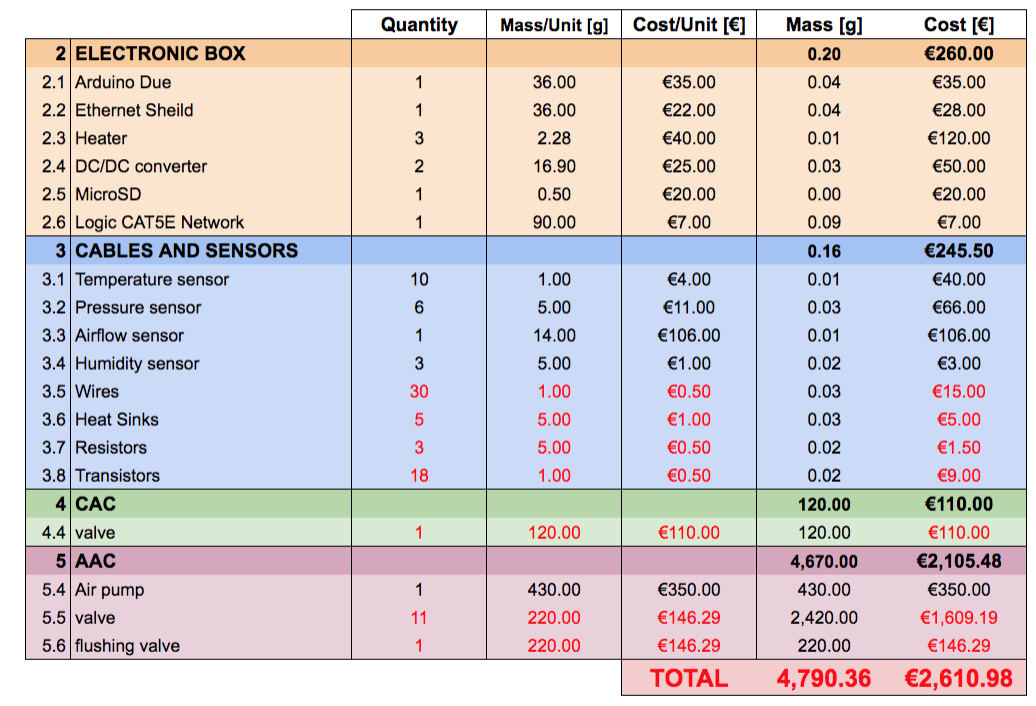
\includegraphics[height=10cm]{4-experiment-design/img/electrical-components-table.png}
%DIF <      \end{align*}
%DIF <      \caption{Table showing all required electrical components.}\label{tab:electrical-components}
%DIF <  \end{table}
\DIFdelbegin %DIFDELCMD < 

%DIFDELCMD < %%%
\DIFdelend \end{landscape}

\begin{landscape}

\subsubsection{Mechanical Components}

Table \DIFdelbegin \DIFdel{\ref{tab:mechanical-components} }\DIFdelend \DIFaddbegin \DIFadd{\ref{tab:components-table-mechanical} }\DIFaddend shows all required mechanical components with \DIFaddbegin \DIFadd{their total }\DIFaddend mass and price.\DIFdelbegin \DIFdel{Table cells highlighted in yellow denote values that have yet to be determined.
}\DIFdelend \DIFaddbegin \\
\DIFaddend 


\DIFdelbegin %DIFDELCMD < \begin{longtable}{|m{0.03\textwidth}|m{0.2\textwidth}|m{0.25\textwidth}|m{0.05\textwidth}|m{0.1\textwidth}|m{0.28\textwidth}|m{0.15\textwidth}|m{0.15\textwidth}|}
%DIFDELCMD <      

%DIFDELCMD <    
%DIFDELCMD < %%%
\DIFdelend \DIFaddbegin \begin{longtable} {\DIFadd{|m}{\DIFadd{0.05\textwidth}}\DIFadd{|m}{\DIFadd{0.25\textwidth}}\DIFadd{|m}{\DIFadd{0.15\textwidth}}\DIFadd{|m}{\DIFadd{0.2\textwidth}}\DIFadd{|m}{\DIFadd{0.05\textwidth}}\DIFadd{|m}{\DIFadd{0.05\textwidth}}\DIFadd{|m}{\DIFadd{0.05\textwidth}}\DIFadd{|m}{\DIFadd{0.25\textwidth}}\DIFadd{|m}{\DIFadd{0.095\textwidth}}\DIFadd{|}} \DIFaddend \hline \textbf{ID} & \textbf{\DIFdelbegin \DIFdel{Components}\DIFdelend \DIFaddbegin \DIFadd{A}\DIFaddend } & \textbf{\DIFdelbegin \DIFdel{Specs (size,weight)}\DIFdelend \DIFaddbegin \DIFadd{B}\DIFaddend } & \textbf{\DIFdelbegin \DIFdel{No.}\DIFdelend \DIFaddbegin \DIFadd{C}\DIFaddend } & \textbf{\DIFdelbegin \DIFdel{Cost}\DIFdelend \DIFaddbegin \DIFadd{D}\DIFaddend } & \textbf{\DIFdelbegin \DIFdel{Note}\DIFdelend \DIFaddbegin \DIFadd{E}\DIFaddend } & \textbf{\DIFdelbegin \DIFdel{Availability}\DIFdelend \DIFaddbegin \DIFadd{F}\DIFaddend }  & \textbf{\DIFdelbegin \DIFdel{Status}\DIFdelend \DIFaddbegin \DIFadd{G}\DIFaddend }  \DIFaddbegin & \textbf{\DIFadd{H}} \DIFaddend \\ \hline \DIFdelbegin \DIFdel{1 }\DIFdelend \DIFaddbegin \DIFadd{M1 }\DIFaddend & \DIFdelbegin \DIFdel{Aluminum Bar }\DIFdelend \DIFaddbegin \DIFadd{Strut profile 20x20 M6/M6, length: 460 mm }\DIFaddend & \DIFdelbegin \DIFdel{45cm }\DIFdelend \DIFaddbegin \DIFadd{Bosch - Rexroth }\DIFaddend & \DIFdelbegin \DIFdel{12 }\DIFdelend \DIFaddbegin \DIFadd{3842993231 }\DIFaddend & \DIFdelbegin \DIFdel{TBD}\footnote{\DIFdel{Budget in Table 3.3.2 has estimated values. TBD here until exact values are figured out. }%DIFDELCMD < \label{fn:mechcomp1}%%%
} %DIFAUXCMD
\addtocounter{footnote}{-1}%DIFAUXCMD
\DIFdelend \DIFaddbegin \DIFadd{16 }\DIFaddend & \DIFaddbegin \DIFadd{180 }& \DIFadd{7.8 }& \DIFaddend Railed geometry, Structural element & \DIFdelbegin \DIFdel{Online }%DIFDELCMD < & %%%
\DIFdel{To be ordered }\DIFdelend \DIFaddbegin \DIFadd{To Be Ordered }\DIFaddend \\ \hline \DIFdelbegin \DIFdel{2 }\DIFdelend \DIFaddbegin \DIFadd{M2 }\DIFaddend & \DIFdelbegin \DIFdel{Aluminum Bar }\DIFdelend \DIFaddbegin \DIFadd{Strut profile 20x20 M6/M6, length: 360 mm }\DIFaddend & \DIFdelbegin \DIFdel{40cm }\DIFdelend \DIFaddbegin \DIFadd{Bosch - Rexroth }\DIFaddend & \DIFdelbegin \DIFdel{8 }\DIFdelend \DIFaddbegin \DIFadd{3842993231 }\DIFaddend & \DIFdelbegin \DIFdel{TBD\textsuperscript{\ref{fn:mechcomp1}} }\DIFdelend \DIFaddbegin \DIFadd{4 }\DIFaddend & \DIFaddbegin \DIFadd{140 }& \DIFadd{7.3 }& \DIFaddend Railed geometry, Structural element & \DIFdelbegin \DIFdel{Online }%DIFDELCMD < & %%%
\DIFdel{To be ordered }\DIFdelend \DIFaddbegin \DIFadd{To Be Ordered }\DIFaddend \\ \hline \DIFdelbegin \DIFdel{3 }\DIFdelend \DIFaddbegin \DIFadd{M3 }\DIFaddend & \DIFdelbegin \DIFdel{Aluminum Bar }\DIFdelend \DIFaddbegin \DIFadd{Strut profile 20x20 M6/M6, length: 190 mm }\DIFaddend & \DIFdelbegin \DIFdel{25cm }\DIFdelend \DIFaddbegin \DIFadd{Bosch - Rexroth }\DIFaddend & \DIFaddbegin \DIFadd{3842993231 }& \DIFaddend 4 & \DIFdelbegin \DIFdel{TBD\textsuperscript{\ref{fn:mechcomp1}} }\DIFdelend \DIFaddbegin \DIFadd{76 }\DIFaddend & \DIFaddbegin \DIFadd{6.8 }& \DIFaddend Railed geometry, Structural element & \DIFdelbegin \DIFdel{Online }%DIFDELCMD < & %%%
\DIFdel{To be ordered }\DIFdelend \DIFaddbegin \DIFadd{To Be Ordered }\DIFaddend \\ \hline \DIFdelbegin \DIFdel{4 }\DIFdelend \DIFaddbegin \DIFadd{M4 }\DIFaddend & \DIFdelbegin \DIFdel{Aluminum Plate }\DIFdelend \DIFaddbegin \DIFadd{T-nut N6 M4 }\DIFaddend & \DIFdelbegin \DIFdel{50 x 40 x 0.2 cm }\DIFdelend \DIFaddbegin \DIFadd{Bosch - Rexroth }\DIFaddend & \DIFdelbegin \DIFdel{4 }\DIFdelend \DIFaddbegin \DIFadd{3842536599 }\DIFaddend & \DIFdelbegin \DIFdel{TBD\textsuperscript{\ref{fn:mechcomp1}} }\DIFdelend \DIFaddbegin \DIFadd{100 }\DIFaddend & \DIFaddbegin \DIFadd{3 }& \DIFadd{0.99 }& \DIFaddend Wall, Protective element & \DIFdelbegin \DIFdel{Store }%DIFDELCMD < & %%%
\DIFdel{To be ordered }\DIFdelend \DIFaddbegin \DIFadd{To Be Ordered }\DIFaddend \\ \hline \DIFdelbegin \DIFdel{5 }\DIFdelend \DIFaddbegin \DIFadd{M5 }\DIFaddend & \DIFdelbegin \DIFdel{Aluminum Plate }\DIFdelend \DIFaddbegin \DIFadd{Sliding block swivel-in N6 M4 }\DIFaddend & \DIFdelbegin \DIFdel{50 x 25 x 0.2 cm }\DIFdelend \DIFaddbegin \DIFadd{Bosch - Rexroth }\DIFaddend & \DIFdelbegin \DIFdel{4 }\DIFdelend \DIFaddbegin \DIFadd{3842536669 }\DIFaddend & \DIFdelbegin \DIFdel{TBD\textsuperscript{\ref{fn:mechcomp1}} }\DIFdelend \DIFaddbegin \DIFadd{100 }\DIFaddend & \DIFaddbegin \DIFadd{3 }& \DIFadd{0.96 }& \DIFaddend Wall, Protective element & \DIFdelbegin \DIFdel{Store }%DIFDELCMD < & %%%
\DIFdel{To be ordered }\DIFdelend \DIFaddbegin \DIFadd{To Be Ordered }\DIFaddend \\ \hline \DIFaddbegin \DIFadd{M6 }& \DIFadd{Bracket standard 20x20 N6/}\DIFaddend 6 & \DIFdelbegin \DIFdel{Aluminum Plate }\DIFdelend \DIFaddbegin \DIFadd{Bosch - Rexroth }\DIFaddend & \DIFdelbegin \DIFdel{50 x 50 x 0.2 cm }\DIFdelend \DIFaddbegin \DIFadd{3842523508 }\DIFaddend & \DIFdelbegin \DIFdel{2 }\DIFdelend \DIFaddbegin \DIFadd{100 }\DIFaddend & \DIFdelbegin \DIFdel{TBD\textsuperscript{\ref{fn:mechcomp1}} }\DIFdelend \DIFaddbegin \DIFadd{5 }\DIFaddend & \DIFaddbegin \DIFadd{0.6 }& \DIFaddend Wall, Protective element & \DIFdelbegin \DIFdel{Store }%DIFDELCMD < & %%%
\DIFdel{To be ordered }\DIFdelend \DIFaddbegin \DIFadd{To Be Ordered }\DIFaddend \\ \hline \DIFdelbegin \DIFdel{7 }\DIFdelend \DIFaddbegin \DIFadd{M7 }\DIFaddend & \DIFdelbegin \DIFdel{Aluminum Plate }\DIFdelend \DIFaddbegin \DIFadd{Variofix block S N6 20x20 }\DIFaddend & \DIFdelbegin \DIFdel{40 x 40 x 0.2 cm }\DIFdelend \DIFaddbegin \DIFadd{Bosch - Rexroth }\DIFaddend & \DIFdelbegin \DIFdel{2 }\DIFdelend \DIFaddbegin \DIFadd{3842548836 }\DIFaddend & \DIFdelbegin \DIFdel{TBD\textsuperscript{\ref{fn:mechcomp1}} }\DIFdelend \DIFaddbegin \DIFadd{70 }\DIFaddend & \DIFaddbegin \DIFadd{5 }& \DIFadd{0.82 }& \DIFaddend Wall, Protective element & \DIFdelbegin \DIFdel{Store }\DIFdelend \DIFaddbegin \DIFadd{To Be Ordered }\\ \hline \DIFadd{M8 }\DIFaddend & \DIFdelbegin \DIFdel{To be ordered }\DIFdelend \DIFaddbegin \DIFadd{Cubic connector 20/3 N6 }& \DIFadd{Bosch - Rexroth }& \DIFadd{3842523872 }& \DIFadd{16 }& \DIFadd{10 }& \DIFadd{2.6 }&  & \DIFadd{To Be Ordered }\DIFaddend \\ \hline \DIFaddbegin \DIFadd{M9 }& \DIFadd{Strap-shaped handle }& \DIFadd{Bosch - Rexroth }& \DIFadd{3842518738 }& \DIFadd{4 }& \DIFadd{20 }& \DIFadd{2.5 }&  & \DIFadd{To Be Ordered }\\ \hline \DIFadd{M10 }& \DIFadd{Retainer ring M4 }& \DIFadd{Bosch - Rexroth }& \DIFadd{3842542328 }& \DIFadd{100 }& \DIFadd{0.5 }& \DIFadd{0.072 }&  & \DIFadd{To Be Ordered }\\ \hline \DIFadd{M11 }& \DIFadd{DIN 7984 M4x8 bolts }& \DIFadd{n/a }& \DIFadd{n/a }& \DIFadd{150 }& \DIFadd{1 }& \DIFadd{0 }&  & \DIFadd{Received }\\ \hline \DIFadd{M12 }& \DIFadd{M6x16 bolts }& \DIFadd{n/a }& \DIFadd{n/a }& \DIFadd{48 }& \DIFadd{5 }& \DIFadd{0 }&  & \DIFadd{Received }\\ \hline \DIFadd{M13 }& \DIFadd{ISO 4762 bolts }& \DIFadd{n/a }& \DIFadd{n/a }& \DIFaddend 8 & \DIFdelbegin \DIFdel{Styrofoam }\DIFdelend \DIFaddbegin \DIFadd{2 }\DIFaddend & \DIFaddbegin \DIFadd{0 }&  & \DIFadd{Received }\\ \hline \DIFadd{M14 }& \DIFadd{Washers }& \DIFadd{n/a }& \DIFadd{n/a }& \DIFadd{20 }& \DIFadd{0.2 }& \DIFadd{0 }&  & \DIFadd{Received }\\ \hline \DIFadd{M15 }& \DIFadd{Aluminum sheets }& \DIFadd{Stena stål }& \DIFadd{204599 }& \DIFadd{1 }& \DIFadd{2500 }& \DIFadd{25 }&  & \DIFadd{To Be Ordered }\\ \hline \DIFadd{M16 }& \DIFadd{Styrofoam 250 SL-A-N }& \DIFadd{Isover }& \DIFadd{3542005000 }& \DIFadd{1 }& \DIFadd{1300 }& \DIFadd{110 }&  & \DIFadd{To Be Ordered }\\ \hline \DIFadd{M17 }& \DIFadd{Fixing bar for the bags }& \DIFadd{Eural }& \DIFadd{148-21-940 }& \DIFaddend 2 \DIFdelbegin \DIFdel{\mbox{%DIFAUXCMD
$m^2$
}%DIFAUXCMD
, 1cm thick }\DIFdelend & \DIFaddbegin \DIFadd{36 }& \DIFadd{5.7 }&  & \DIFadd{To Be Ordered }\\ \hline \DIFadd{M18 }& \DIFadd{Flat plate interface for fixing bar }& \DIFadd{Stena stål }& \DIFadd{n/a }& \DIFadd{4 }& \DIFadd{32 }& \DIFadd{2 }&  & \DIFadd{To Be Ordered }\\ \hline \DIFadd{M19 }& \DIFadd{CAC-AAC interface 6-hole plate }& \DIFadd{Stena stål }& \DIFadd{n/a }& \DIFadd{4 }& \DIFadd{50 }& \DIFadd{2 }&  & \DIFadd{To Be Ordered }\\ \hline \DIFadd{M20 }& \DIFadd{Aluminum sheets }& \DIFadd{Stena stål }& \DIFadd{204599 }& \DIFaddend 1 & \DIFdelbegin \DIFdel{TBD\textsuperscript{\ref{fn:mechcomp1}} }\DIFdelend \DIFaddbegin \DIFadd{100 }\DIFaddend & \DIFdelbegin \DIFdel{Wall, Protective element }\DIFdelend \DIFaddbegin \DIFadd{NaN }\DIFaddend &  \DIFdelbegin \DIFdel{Store }\DIFdelend & \DIFdelbegin \DIFdel{To be ordered }\DIFdelend \DIFaddbegin \DIFadd{To Be Ordered }\DIFaddend \\ \hline \DIFdelbegin \DIFdel{9 }\DIFdelend \DIFaddbegin \DIFadd{M21 }\DIFaddend & \DIFdelbegin \DIFdel{Polyethylene foam }\DIFdelend \DIFaddbegin \DIFadd{Stainless Steel 304, Equal Angle bar 2 m }\DIFaddend & \DIFaddbegin \DIFadd{Hardware warehouse }& \DIFadd{HW1200 }& \DIFadd{1 }& \DIFadd{380 }& \DIFadd{31 }&  & \DIFadd{To Be Ordered }\\ \hline \DIFadd{M22 }& \DIFadd{DIN 7984 M4x8 bolts }& \DIFadd{n/a }& \DIFadd{n/a }& \DIFadd{30 }& \DIFadd{1 }& \DIFadd{0 }&  & \DIFadd{Received }\\ \hline \DIFadd{M23 }& \DIFadd{DIN 7984 M4x30 bolts }& \DIFadd{n/a }& \DIFadd{n/a }& \DIFadd{4 }& \DIFaddend 2 \DIFdelbegin \DIFdel{\mbox{%DIFAUXCMD
$m^2$
}%DIFAUXCMD
, 1cm thick }\DIFdelend & \DIFaddbegin \DIFadd{0 }&  & \DIFadd{Received }\\ \hline \DIFadd{M24 }& \DIFadd{Nut M4 }& \DIFadd{n/a }& \DIFadd{n/a }& \DIFadd{34 }& \DIFaddend 1 & \DIFdelbegin \DIFdel{TBD\textsuperscript{\ref{fn:mechcomp1}} }\DIFdelend \DIFaddbegin \DIFadd{0 }\DIFaddend &  \DIFdelbegin \DIFdel{Wall, Thermal insulation }\DIFdelend & \DIFdelbegin \DIFdel{Store }\DIFdelend \DIFaddbegin \DIFadd{Received }\\ \hline \DIFadd{M25 }\DIFaddend & \DIFdelbegin \DIFdel{To be ordered }\DIFdelend \DIFaddbegin \DIFadd{Flat plate fixing interface }& \DIFadd{n/a }& \DIFadd{n/a }& \DIFadd{2 }& \DIFadd{1 }& \DIFadd{0 }&  & \DIFadd{To Be Ordered }\DIFaddend \\ \hline %DIF < 9 & Bag Valves & \textit{Swagelok} & 16 & TBD\textsuperscript{\ref{fn:mechcomp1}} & Interface bags with tubes & Online & To be ordered \\ \hline
\DIFdelbegin \DIFdel{10 }\DIFdelend \DIFaddbegin \DIFadd{M26 }\DIFaddend & \DIFdelbegin \DIFdel{Corner joint }\DIFdelend \DIFaddbegin \DIFadd{7mm Standoff/Spacer for PCB }\DIFaddend & \DIFaddbegin \DIFadd{ETTINGER }& \DIFadd{05.13.071  }& \DIFadd{5 }& \DIFadd{2 }& \DIFadd{0.4 }&  & \DIFadd{To Be Ordered }\\ \hline \DIFadd{M27 }& \DIFadd{Lock nut M3 (DIN985) for PCB }& \DIFadd{Clas ohlson }& \DIFadd{11-1936-3 }& \DIFadd{5 }& \DIFadd{1 }& \DIFaddend 0.2 \DIFdelbegin \DIFdel{x 0.2 cm }\DIFdelend &  \DIFdelbegin \DIFdel{52 }\DIFdelend & \DIFdelbegin \DIFdel{TBD\textsuperscript{\ref{fn:mechcomp1}} }\DIFdelend \DIFaddbegin \DIFadd{To Be Ordered }\\ \hline \DIFadd{M28 }\DIFaddend & \DIFdelbegin \DIFdel{Join structure bars,  90-degree angle }\DIFdelend \DIFaddbegin \DIFadd{M3 Cheese Head Screws (DIN 84) for PCB,  }\DIFaddend & \DIFdelbegin \DIFdel{Online }\DIFdelend \DIFaddbegin \DIFadd{Accu }\DIFaddend & \DIFdelbegin \DIFdel{To be ordered }\DIFdelend \DIFaddbegin \DIFadd{SFE-M3-4-A4 }& \DIFadd{5 }& \DIFadd{0.8 }& \DIFadd{0.7 }&  & \DIFadd{To Be Ordered }\DIFaddend \\ \hline %DIF < 11 & Electronics shielding box & 20 x 10 x 10 cm & 1 & TBD\textsuperscript{\ref{fn:mechcomp2}} & Electronics center & Store & To be built \\ \hline
%DIF < 11 & Coated box & 20 x 10 x 10 cm & 1 & TBD\textsuperscript{\ref{fn:mechcomp2}} & Valve center for AAC & Store & To be built \\ \hline
%DIF < 12 & Plastic Tube & 5 m & 1 & TBD\textsuperscript{\ref{fn:mechcomp2}} & Valves to bags & Store & To be ordered \\ \hline
%DIF < 13 & Air Filter & TBD\textsuperscript{\ref{fn:mechcomp2}} & 1 & TBD\textsuperscript{\ref{fn:mechcomp2}} & Main pipe protection & Store & To be built \\ \hline
\DIFdelbegin \DIFdel{11 }\DIFdelend \DIFaddbegin \DIFadd{M29 }\DIFaddend & \DIFdelbegin \DIFdel{Flange }\DIFdelend \DIFaddbegin \DIFadd{Coiled tube }\DIFaddend & \DIFdelbegin \DIFdel{Small }\DIFdelend \DIFaddbegin \DIFadd{FMI }\DIFaddend & \DIFdelbegin \DIFdel{50 }\DIFdelend \DIFaddbegin \DIFadd{n/a }\DIFaddend & \DIFdelbegin \DIFdel{TBD\textsuperscript{\ref{fn:mechcomp1}} }\DIFdelend \DIFaddbegin \DIFadd{1 }\DIFaddend & \DIFdelbegin \DIFdel{Join tubes with valves }\DIFdelend \DIFaddbegin \DIFadd{5000 }\DIFaddend & \DIFdelbegin \DIFdel{Store }\DIFdelend \DIFaddbegin \DIFadd{22000 }\DIFaddend &  \DIFdelbegin \DIFdel{To be ordered }\DIFdelend \DIFaddbegin & \DIFadd{To Be Delivered }\DIFaddend \\ \hline \DIFdelbegin \DIFdel{12 }\DIFdelend \DIFaddbegin \DIFadd{M30 }\DIFaddend & \DIFdelbegin \DIFdel{Bar }\DIFdelend \DIFaddbegin \DIFadd{Interface tube-screw male (OD 1/4" - ID 5/32" to male 1/4") }\DIFaddend & \DIFaddbegin \DIFadd{SMC }& \DIFadd{KFG2H0704-N02S }& \DIFadd{1 }& \DIFadd{19 }& \DIFadd{20 }&  & \DIFadd{To Be Ordered }\\ \hline \DIFadd{M31 }& \DIFadd{Interface tube-screw male (OD 1/4" - ID 5/32" to male 1/8") }& \DIFadd{SMC }& \DIFadd{KFG2H0704-N01S }& \DIFadd{1 }& \DIFadd{13 }& \DIFadd{20 }&  & \DIFadd{To Be Ordered }\\ \hline \DIFadd{M32 }& \DIFadd{Interface reducing adapters (female 1/4" NPT to male 1/8"  NPT) }& \DIFadd{Swagelok }& \DIFadd{SS-4-RA-2 }& \DIFadd{1 }& \DIFadd{35 }& \DIFadd{20 }&  & \DIFadd{To Be Ordered }\\ \hline \DIFadd{M33 }& \DIFadd{Interface attached to the coiled tube outlet, quick connector }& \DIFadd{Swagelok }& \DIFadd{SS-QC4-B-200 }& \DIFadd{1 }& \DIFadd{91 }& \DIFadd{48 }&  & \DIFadd{To Be Ordered }\\ \hline \DIFadd{M34 }& \DIFadd{Interface attached to the coiled tube inlet, quick connector }& \DIFadd{Swagelok }& \DIFadd{SS-QC4-B-400 }& \DIFadd{1 }& \DIFadd{68 }& \DIFadd{20 }&  & \DIFadd{To Be Ordered }\\ \hline \DIFadd{M35 }& \DIFadd{Interface quick connector stem with valve }& \DIFadd{Swagelok }& \DIFadd{SS-QC4-D-400 }& \DIFadd{1 }& \DIFadd{58 }& \DIFadd{35 }&  & \DIFadd{To Be Ordered }\\ \hline \DIFadd{M36 }& \DIFadd{Interface Female 1/4" Quick Coupling for T-Union }& \DIFadd{Swagelok }& \DIFadd{SS-QC4-B-4PF }& \DIFadd{8 }& \DIFaddend 45 \DIFdelbegin \DIFdel{x 0.8 cm }\DIFdelend & \DIFaddbegin \DIFadd{55 }&  & \DIFadd{To Be Ordered }\\ \hline \DIFadd{M37 }& \DIFadd{Testing / Backup seal valve }& \DIFadd{Parker }& \DIFadd{4M4F-V6LN-SS }& \DIFaddend 2 & \DIFdelbegin \DIFdel{TBD\textsuperscript{\ref{fn:mechcomp1}} }\DIFdelend \DIFaddbegin \DIFadd{1400 }\DIFaddend & \DIFdelbegin \DIFdel{Anchor point fro bags }\DIFdelend \DIFaddbegin \DIFadd{150 }\DIFaddend &  \DIFdelbegin \DIFdel{Store }\DIFdelend & \DIFdelbegin \DIFdel{To be ordered }\DIFdelend \DIFaddbegin \DIFadd{Received }\DIFaddend \\ \hline \DIFaddbegin \DIFadd{M38 }& \DIFadd{Magnesium filter with interface }& \DIFadd{FMI }& \DIFadd{n/a }& \DIFadd{1 }& \DIFadd{65 }& \DIFadd{150 }&  & \DIFadd{Ordered }\\ \hline \DIFadd{M39 }& \DIFadd{Testing Valve  }& \DIFadd{Axel Larsson }& \DIFadd{Lucifer 121K, 122K }& \DIFadd{1 }& \DIFadd{NaN }& \DIFadd{100 }&  & \DIFadd{Received }\\ \hline \DIFadd{M40 }& \DIFadd{Gas Sampling Bag, Multi-Layer Foil, 3L, 10"x10", 5pk }& \DIFadd{Restek }& \DIFadd{22951 }& \DIFadd{2 }& \DIFadd{25 }& \DIFadd{100 }&  & \DIFadd{To Be Ordered }\\ \hline \DIFadd{M41 }& \DIFadd{Interface tube-screw male (OD 1/4" - ID 5/32" to male 1/8") }& \DIFadd{SMC }& \DIFadd{KFG2H0704-N01S }& \DIFadd{12 }& \DIFaddend 13 & \DIFdelbegin \DIFdel{Handle }\DIFdelend \DIFaddbegin \DIFadd{20 }\DIFaddend &  \DIFdelbegin \DIFdel{TBD}\footnote{\DIFdel{Exact size depending on availability. }%DIFDELCMD < \label{fn:mechcomp2}%%%
} %DIFAUXCMD
\addtocounter{footnote}{-1}%DIFAUXCMD
\DIFdelend & \DIFaddbegin \DIFadd{To Be Ordered }\\ \hline \DIFadd{M42 }& \DIFadd{Straight Union  (OD 1/}\DIFaddend 4\DIFaddbegin \DIFadd{" - ID 5/32") }\DIFaddend & \DIFdelbegin \DIFdel{TBD\textsuperscript{\ref{fn:mechcomp1}} }\DIFdelend \DIFaddbegin \DIFadd{SMC }\DIFaddend & \DIFdelbegin \DIFdel{Experiment box manipulation }\DIFdelend \DIFaddbegin \DIFadd{KFG2H0704-00 }\DIFaddend & \DIFdelbegin \DIFdel{Store }\DIFdelend \DIFaddbegin \DIFadd{3 }\DIFaddend & \DIFdelbegin \DIFdel{To be ordered }\DIFdelend \DIFaddbegin \DIFadd{16 }& \DIFadd{20 }&  & \DIFadd{To Be Ordered }\DIFaddend \\ \hline \DIFaddbegin \DIFadd{M43 }& \DIFadd{Interface tube-screw female (OD 1/4" - ID 5/32" to female 1/4") }& \DIFadd{SMC }& \DIFadd{KFG2F0704-N02 }& \DIFadd{3 }& \DIFadd{28 }& \DIFadd{20 }&  & \DIFadd{To Be Ordered }\\ \hline \DIFadd{M44 }& \DIFadd{T-Union }& \DIFadd{Swagelok }& \DIFadd{SS-400-3 }& \DIFadd{8 }& \DIFadd{71 }& \DIFadd{33 }&  & \DIFadd{To Be Ordered }\\ \hline \DIFadd{M45 }& \DIFadd{Nut Ferrule set (50pcs) }& \DIFadd{Swagelok }& \DIFadd{SS-400-NFSET }& \DIFadd{16 }& \DIFadd{41 }& \DIFadd{2.3 }&  & \DIFadd{To Be Ordered }\\ \hline \DIFadd{M46 }& \DIFadd{Tubing, Sulfinert 304SS Welded/Drawn 20ft (OD 1/4" - ID 0,21") }& \DIFadd{Restek }& \DIFadd{29255 }& \DIFadd{1 }& \DIFadd{150 }& \DIFadd{350 }&  & \DIFadd{To Be Ordered }\\ \hline \DIFadd{M47 }& \DIFadd{Quick Coupling female 1/4" }& \DIFadd{Swagelok }& \DIFadd{SS-QC4-B-4PF }& \DIFadd{6 }& \DIFadd{45 }& \DIFadd{50 }&  & \DIFadd{To Be Ordered }\\ \hline \DIFadd{M48 }& \DIFadd{Cap }& \DIFadd{Swagelok }& \DIFadd{SS-200-C }& \DIFadd{2 }& \DIFadd{20 }& \DIFadd{10 }&  & \DIFadd{To Be Ordered }\\ \hline \DIFadd{M49 }& \DIFadd{Aluminum tube for sensors }& \DIFadd{n/a }& \DIFadd{n/a }& \DIFadd{1 }& \DIFadd{200 }& \DIFadd{- }& \DIFadd{Need to be custom ordered }& \DIFadd{To Be Ordered }\\ \hline \DIFadd{M50 }& \DIFadd{Magnesium filter tube with interface }& \DIFadd{FMI }& \DIFadd{- }& \DIFadd{1 }& \DIFadd{65 }& \DIFadd{150 }&  & \DIFadd{Ordered }\\ \hline \DIFadd{M51 }& \DIFadd{Manifold (inlet and outlet 1/8" female) }& \DIFadd{SMC }& \DIFadd{VV2DW2-H0801N-F-Q }& \DIFadd{1 }& \DIFadd{440 }& \DIFadd{140 }&  & \DIFadd{To Be Ordered }\\ \hline \DIFadd{M52 }& \DIFadd{Aluminum flat bar 258 mm long 20 mm wide t = 1 mm }& \DIFadd{n/a }& \DIFadd{n/a }& \DIFadd{4 }& \DIFaddend 14 & \DIFdelbegin \DIFdel{Screw }\DIFdelend \DIFaddbegin \DIFadd{4 }\DIFaddend &  \DIFdelbegin \DIFdel{TBD\textsuperscript{\ref{fn:mechcomp2}} }\DIFdelend & \DIFdelbegin \DIFdel{160 }\DIFdelend \DIFaddbegin \DIFadd{To Be Ordered }\\ \hline \DIFadd{M53 }\DIFaddend & \DIFdelbegin \DIFdel{TBD\textsuperscript{\ref{fn:mechcomp1}} }\DIFdelend \DIFaddbegin \DIFadd{Aluminum flat bar 146 mm long }\DIFaddend & \DIFdelbegin \DIFdel{Fixing elements }\DIFdelend \DIFaddbegin \DIFadd{n/a }\DIFaddend & \DIFdelbegin \DIFdel{Store }\DIFdelend \DIFaddbegin \DIFadd{n/a }\DIFaddend & \DIFdelbegin \DIFdel{To be ordered }\DIFdelend \DIFaddbegin \DIFadd{1 }& \DIFadd{7.8 }& \DIFadd{4 }&  & \DIFadd{To Be Ordered }\DIFaddend \\ \hline \DIFdelbegin %DIFDELCMD < 

%DIFDELCMD <     %%%
\DIFdelend \caption{\DIFaddbegin \DIFadd{Mechanical Components }\DIFaddend Table\DIFdelbegin \DIFdel{showing all required mechanical components}\DIFdelend } \DIFdelbegin %DIFDELCMD < \label{tab:mechanical-components}
%DIFDELCMD < %%%
\DIFdelend \DIFaddbegin \label{tab:components-table-mechanical} \DIFaddend \end{longtable} \raggedbottom

%DIF < \begin{table}[H]
%DIF < %    \begin{align*}
%DIF <         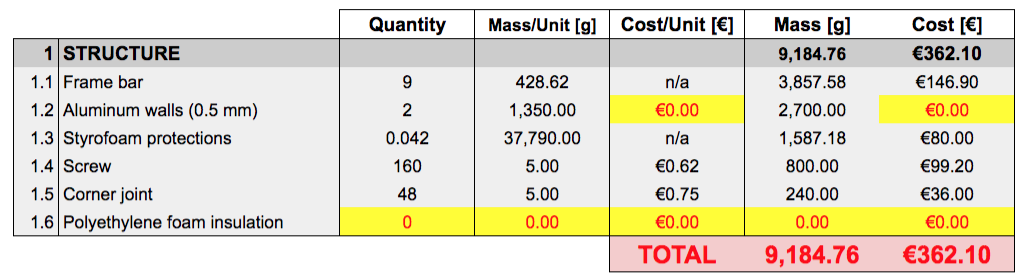
\includegraphics{4-experiment-design/img/mechanical-components-table.png}
%DIF <     \end{align*}
%DIF <     \caption{Table showing all required mechanical components.}\label{tab:mechanical-components}
%DIF < \end{table}
\DIFdelbegin %DIFDELCMD < 

%DIFDELCMD < %%%
\DIFdelend \DIFaddbegin \raggedbottom
\DIFaddend \end{landscape}

\DIFaddbegin \begin{landscape}
\DIFaddend \subsubsection{Other Components}
\DIFaddbegin \DIFadd{Table \ref{tab:component-table-other} shows other components which contribute to the mass and/or price.}\\
\DIFaddend 

\DIFdelbegin \DIFdel{Other components are included in the full budget previously presented in Table \ref{tab:budget-table}.}\DIFdelend \DIFaddbegin \begin{longtable} {\DIFadd{|m}{\DIFadd{0.05\textwidth}}\DIFadd{|m}{\DIFadd{0.25\textwidth}}\DIFadd{|m}{\DIFadd{0.15\textwidth}}\DIFadd{|m}{\DIFadd{0.2\textwidth}}\DIFadd{|m}{\DIFadd{0.05\textwidth}}\DIFadd{|m}{\DIFadd{0.05\textwidth}}\DIFadd{|m}{\DIFadd{0.05\textwidth}}\DIFadd{|m}{\DIFadd{0.25\textwidth}}\DIFadd{|m}{\DIFadd{0.095\textwidth}}\DIFadd{|}} \hline \textbf{\DIFadd{ID}} & \textbf{\DIFadd{A}} & \textbf{\DIFadd{B}} & \textbf{\DIFadd{C}} & \textbf{\DIFadd{D}} & \textbf{\DIFadd{E}} & \textbf{\DIFadd{F}}  & \textbf{\DIFadd{G}}  & \textbf{\DIFadd{H}} \\ \hline \DIFadd{O1 }& \DIFadd{Tubing Bender }& \DIFadd{Restek }& \DIFadd{23009 }& \DIFadd{1 }& \DIFadd{n/a }& \DIFadd{110 }&  & \DIFadd{To Be Ordered }\\ \hline \DIFadd{O2 }& \DIFadd{Ridgid Tubing Cutter for 1/8" or 1/4" metal tubing }& \DIFadd{Restek }& \DIFadd{23011 }& \DIFadd{1 }& \DIFadd{n/a }& \DIFadd{50 }&  & \DIFadd{To Be Ordered }\\ \hline \DIFadd{O3 }& \DIFadd{Tool, 1/8" and 1/4" Tubing Reamer }& \DIFadd{Restek }& \DIFadd{20134 }& \DIFadd{1 }& \DIFadd{n/a }& \DIFadd{45 }&  & \DIFadd{To Be Ordered }\\ \hline \DIFadd{O4 }& \DIFadd{Travel to FMI for sample bag testing }& \DIFadd{n/a }& \DIFadd{n/a }& \DIFadd{1 }& \DIFadd{n/a }& \DIFadd{250 }&  & \DIFadd{Completed }\\ \hline \DIFadd{O5 }& \DIFadd{Travel to FMI for integration testing }& \DIFadd{n/a }& \DIFadd{n/a }& \DIFadd{1 }& \DIFadd{n/a }& \DIFadd{250 }&  & \DIFadd{Planned }\\ \hline \DIFadd{O6 }& \DIFadd{Shipping costs }& \DIFadd{n/a }& \DIFadd{n/a }& \DIFadd{n/a }& \DIFadd{n/a }& \DIFadd{n/a }&  & \DIFadd{n/a }\\ \hline \DIFadd{O7 }& \DIFadd{Error margin }& \DIFadd{n/a }& \DIFadd{n/a }& \DIFadd{n/a }& \DIFadd{n/a }& \DIFadd{n/a }&  & \DIFadd{n/a }\\ \hline \caption{\DIFadd{Other Components Table}} \label{tab:component-table-other} \end{longtable} \raggedbottom
\DIFaddend 


\raggedbottom
\DIFaddbegin \end{landscape}
\DIFaddend \pagebreak
\subsection{Mechanical Design} \label{Mechanical_Design}

 \DIFaddbegin \begin{figure}[H]
     \centering
     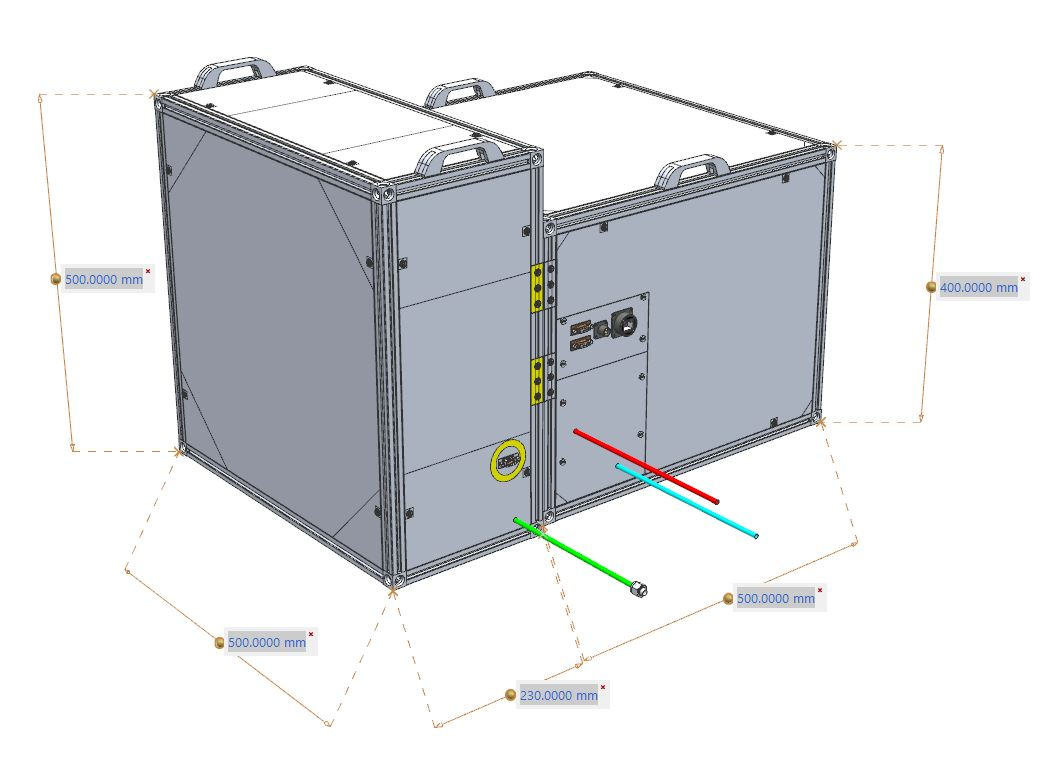
\includegraphics[width=1\textwidth]{4-experiment-design/img/Mechanical/tubular_dimensions.jpg}
     \caption{\DIFaddFL{General Dimensions of the Experiment.}}
     \label{dimensions}
\end{figure}

\begin{table}[H]
\noindent\DIFaddFL{\makebox[\columnwidth]{%
\scalebox{0.8}{
\begin{tabular}{c|c|c|c|}
\cline{2-4}
 & CAC & AAC & TOTAL \\ \hline
\multicolumn{1}{|c|}{Experiment mass {[}kg{]}} & 12.08 & 12.37 & 24.45 \\ \hline
\multicolumn{1}{|c|}{Experiment dimensions {[}m{]}} & \mbox{%DIFAUXCMD
$0.23\ x\ 0.5\ x\ 0.5$
}%DIFAUXCMD
& \mbox{%DIFAUXCMD
$0.5\ x\ 0.5\ x\ 0.4$
}%DIFAUXCMD
& \mbox{%DIFAUXCMD
$0.73\ x\ 0.5\ x\ 0.5$
}%DIFAUXCMD
\\ \hline
\multicolumn{1}{|c|}{Experiment footprint area {[}m^2{]}} & \mbox{%DIFAUXCMD
$0.115$
}%DIFAUXCMD
& \mbox{%DIFAUXCMD
$0.25$
}%DIFAUXCMD
& \mbox{%DIFAUXCMD
$0.365$
}%DIFAUXCMD
\\ \hline
\multicolumn{1}{|c|}{Experiment volume {[}m^3{]}} & \mbox{%DIFAUXCMD
$0.0575$
}%DIFAUXCMD
& \mbox{%DIFAUXCMD
$0.1$
}%DIFAUXCMD
& \mbox{%DIFAUXCMD
$0.1575$
}%DIFAUXCMD
\\ \hline
\multicolumn{1}{|c|}{Experiment expected COG position} & \begin{tabular}[c]{@{}l@{}}\mbox{%DIFAUXCMD
$X=23.51\ cm$
}%DIFAUXCMD
\\ \mbox{%DIFAUXCMD
$Y=10\ cm$
}%DIFAUXCMD
\\ \mbox{%DIFAUXCMD
$Z=22.57\ cm$
}%DIFAUXCMD
\end{tabular}  & \begin{tabular}[c]{@{}l@{}} \mbox{%DIFAUXCMD
$X=29.04\ cm$
}%DIFAUXCMD
\\ \mbox{%DIFAUXCMD
$Y=16.63\ cm$
}%DIFAUXCMD
\\  \mbox{%DIFAUXCMD
$Z=16.2\ cm$
}%DIFAUXCMD
\end{tabular} &\begin{tabular}[c]{@{}l@{}} \mbox{%DIFAUXCMD
$X=26.31\ cm$
}%DIFAUXCMD
\\ \mbox{%DIFAUXCMD
$Y=24.99\ cm$
}%DIFAUXCMD
\\  \mbox{%DIFAUXCMD
$Z=19.35\ cm$
}%DIFAUXCMD
\end{tabular} \\ \hline
\end{tabular}}}
}\caption{\DIFaddFL{Experiment Summary Table}}
\label{table:experiment-summary}
\end{table}


\DIFadd{As it is mentioned in Table \ref{table:experiment-summary}, the Center Of Gravity for the whole experiment appears to be located just on base of the third level of The Brain which coincides with the location of the electronics PCB. This outcome is quite advantageous in terms of stability for one of the most sensitive subsystems of the experiment in terms of shakes and loads. Notice that the values for the center of gravity are based on the reference axis shown in Figure \ref{COG}. Also, the table weights of the boxes and, therefore, the whole experiment, are increased by a \mbox{%DIFAUXCMD
$10\%$
}%DIFAUXCMD
of safety margin.
}

 \begin{figure}[H]
     \centering
     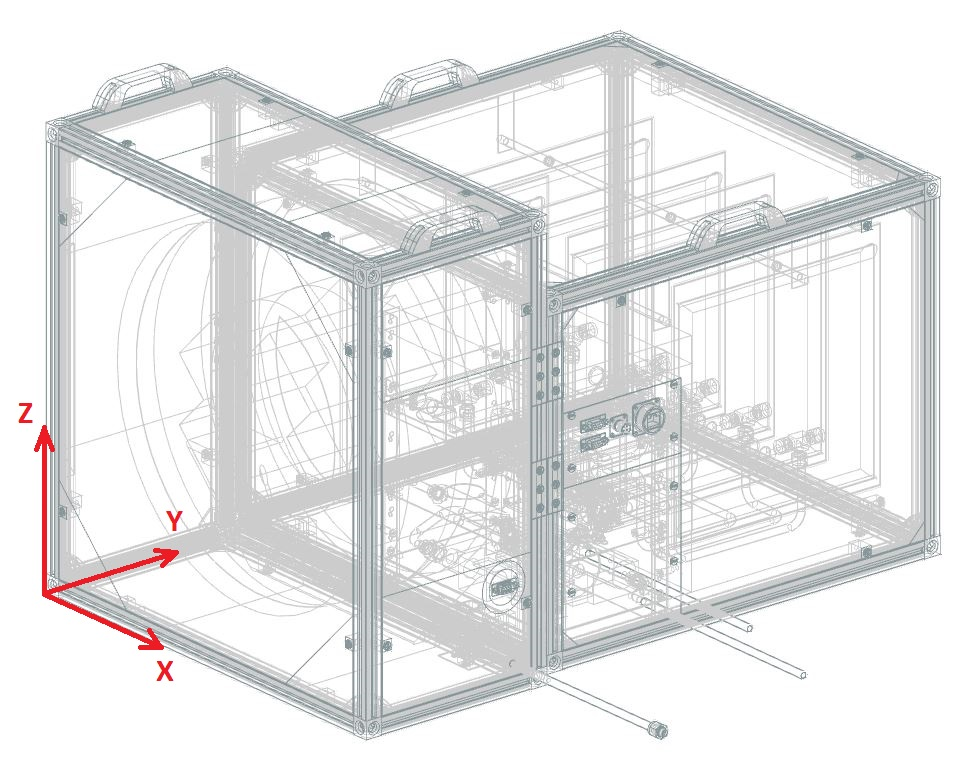
\includegraphics[width=0.7\textwidth]{4-experiment-design/img/Mechanical/COG.jpg}
     \caption{\DIFaddFL{Reference Axis for the Total Center of Gravity.}}
     \label{COG}
\end{figure}

\DIFaddend \subsubsection{Structure}
\DIFaddbegin \label{sec:4.4.1}
\DIFaddend 

The experiment consists \DIFdelbegin \DIFdel{on two cubic }\DIFdelend \DIFaddbegin \DIFadd{of two rectangular }\DIFaddend boxes, one stacked next to the other. The \DIFdelbegin \DIFdel{smallest box -in red in Figure \ref{overview}}\DIFdelend \DIFaddbegin \DIFadd{higher but narrower box }\DIFaddend - \DIFaddbegin \DIFadd{CAC box - }\DIFaddend allocates the heaviest element, the CAC. The main \DIFdelbegin \DIFdel{box-in grey in Figure \ref{overview}}\DIFdelend \DIFaddbegin \DIFadd{box }\DIFaddend - \DIFaddbegin \DIFadd{AAC box - }\DIFaddend contains the AAC system as well as the \DIFdelbegin \DIFdel{general Electronic Box }\DIFdelend \DIFaddbegin \DIFadd{central command unit: The Brain. The Brain contains the general Electronic box }\DIFaddend (EB) \DIFaddbegin \DIFadd{as well as the pneumatic sampling system}\DIFaddend . The frame of these two boxes will be made of aluminum bars which have a characteristic cross-section of 20x20 mm\DIFdelbegin \DIFdel{, see Figure \ref{cross-section}}\DIFdelend . The rails will allow an easy interface between bars and other elements.
\DIFdelbegin \DIFdel{Bars will be joined together by using 90-degree angles and corner cubes, see Figure \ref{3_bars_joined}.
}\DIFdelend 

%DIF < % Cross section of one aluminum bar
%DIF >  % Figure of 3 bars

 \DIFdelbegin %DIFDELCMD < \begin{figure}[!ht]
%DIFDELCMD <     %%%
\DIFdelendFL \DIFaddbeginFL \begin{figure}[H]
     \DIFaddendFL \centering
     \DIFdelbeginFL %DIFDELCMD < 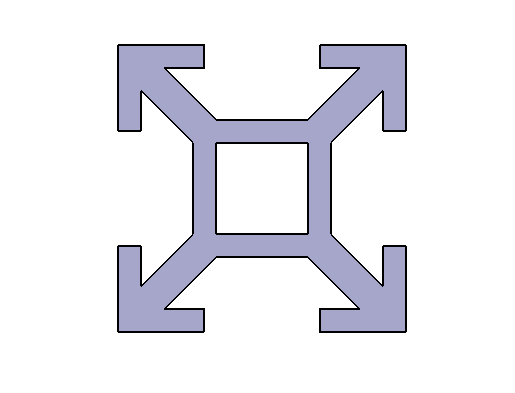
\includegraphics[width=0.5\textwidth]{4-experiment-design/img/1_cross_section.jpg}
%DIFDELCMD <     %%%
\DIFdelendFL \DIFaddbeginFL 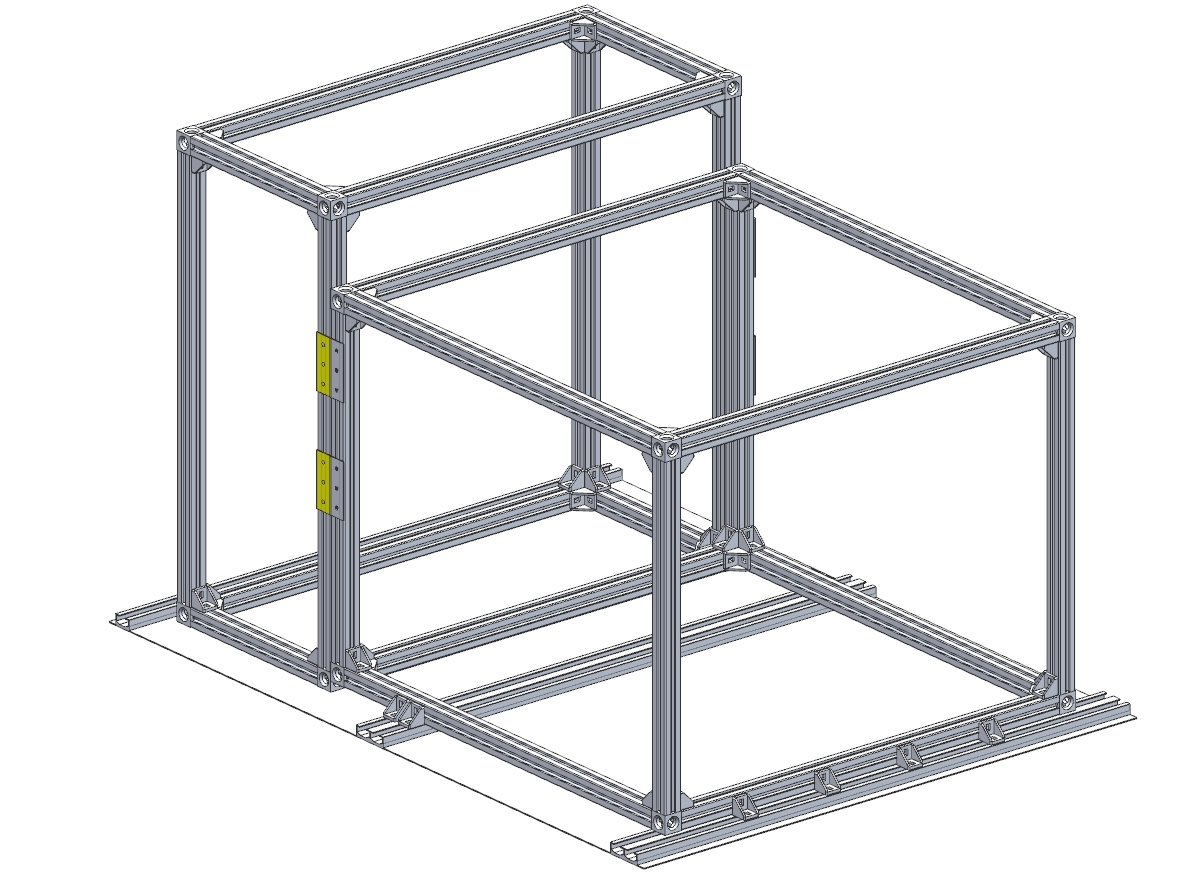
\includegraphics[width=0.9\textwidth]{4-experiment-design/img/Mechanical/structure_pic.jpg}
     \DIFaddendFL \caption{\DIFdelbeginFL \DIFdelFL{Cross section of the structural bars}\DIFdelendFL \DIFaddbeginFL \DIFaddFL{Structure Overview}\DIFaddendFL .}
     \DIFdelbeginFL %DIFDELCMD < \label{cross-section}
%DIFDELCMD < %%%
\DIFdelendFL \DIFaddbeginFL \label{structure}
\DIFaddendFL \end{figure}

%DIF <  Figure of 3 bars
\DIFdelbegin %DIFDELCMD < 

%DIFDELCMD < \begin{figure}[!ht]
%DIFDELCMD <     \centering
%DIFDELCMD <     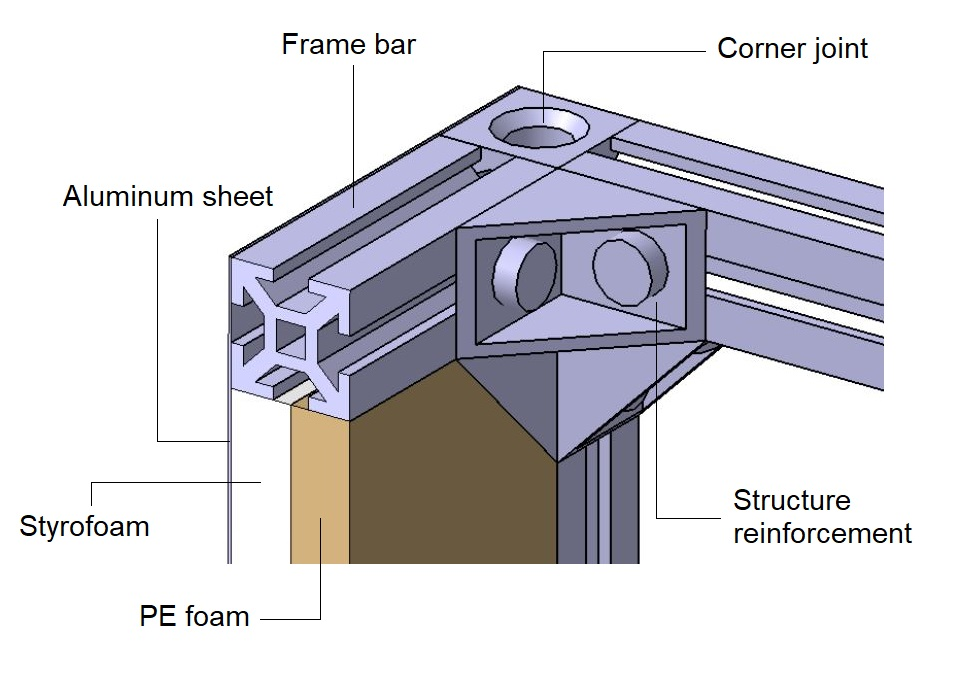
\includegraphics[width=0.8\textwidth]{4-experiment-design/img/structure_cut_name.jpg}
%DIFDELCMD <     %%%
%DIFDELCMD < \caption{%
{%DIFAUXCMD
\DIFdelFL{Interface between structural bars.}}
    %DIFAUXCMD
%DIFDELCMD < \label{3_bars_joined}
%DIFDELCMD < \end{figure}
%DIFDELCMD < 

%DIFDELCMD < %%%
\DIFdelend The frame is designed to withstand all vibrations and ensure a reliable stability of the entire system. \DIFdelbegin \DIFdel{Further tests }\DIFdelend \DIFaddbegin \DIFadd{Test 9 in Table \ref{tab:vibration-test} }\DIFaddend will help to confirm \DIFdelbegin \DIFdel{and update the design }\DIFdelend \DIFaddbegin \DIFadd{the frame can withstand these vibrations and updates to the design will be made }\DIFaddend if necessary. 

The \DIFaddbegin \DIFadd{frame of the structure, shown in Figure \ref{structure}, is built by the aforesaid aluminum strut profiles which are connected to each other with cubic connectors 20/3 that provide better strength and stability for the whole structure. These two components are connected by M6x16 normalized bolts aligned with the bars axis. At the same time, these nodes will be reinforced by three brackets (see Figure \ref{fig:bracket}) each.
}

\DIFadd{Table \ref{table:materials_prop} shows the main properties of the materials used to manufacture the main structural components.
}




\begin{longtable}{|m{0.12\textwidth}| m{0.2\textwidth} |m{0.12\textwidth} |m{0.11\textwidth}|m{0.11\textwidth}| m{0.11\textwidth} | m{0.12\textwidth}|}
\hline
\textbf{\DIFadd{Material}} & \textbf{\DIFadd{Application}} & \textbf{\DIFadd{Density}} & \textbf{\DIFadd{Tensile strength}} & \textbf{\DIFadd{Yield Strength}} & \textbf{\DIFadd{Modulus of elasticity}}  & \textbf{\DIFadd{Brinell hardness}} \\ \hline 
\DIFadd{Aluminium 5754 }& \DIFadd{Wall sheets,  brain structure plates, CAC-AAC join plate }& \DIFadd{\mbox{%DIFAUXCMD
$2.67 g/cm^3$
}%DIFAUXCMD
}& \DIFadd{\mbox{%DIFAUXCMD
$190 MPa$
}%DIFAUXCMD
}& \DIFadd{\mbox{%DIFAUXCMD
$80 MPa$
}%DIFAUXCMD
}& \DIFadd{\mbox{%DIFAUXCMD
$70 GPa$
}%DIFAUXCMD
}& \DIFadd{\mbox{%DIFAUXCMD
$77 HB$
}%DIFAUXCMD
}\\ \hline
\DIFadd{Aluminium 6105-T5 }& \DIFadd{Strut profiles }& \DIFadd{\mbox{%DIFAUXCMD
$2.7g/cm^3$
}%DIFAUXCMD
}& \DIFadd{\mbox{%DIFAUXCMD
$310 MPa$
}%DIFAUXCMD
}& \DIFadd{\mbox{%DIFAUXCMD
$275MPa$
}%DIFAUXCMD
}& \DIFadd{\mbox{%DIFAUXCMD
$69 GPa$
}%DIFAUXCMD
}& \DIFadd{\mbox{%DIFAUXCMD
$95HB$
}%DIFAUXCMD
}\\ \hline

\caption{\DIFadd{Main structural materials}}
\label{table:materials_prop}
\end{longtable}





\DIFadd{The }\DIFaddend two-box design will allow ease of access and manipulation of both the CAC and AAC subsystems, see Figure \DIFdelbegin \DIFdel{\ref{overview}}\DIFdelend \DIFaddbegin \DIFadd{\ref{fig:3D_tubular_render}}\DIFaddend . In addition, the AAC sampling system is designed to be re-usable for future handover to FMI, as such, it will be mountable on any standard balloon flight without having to introduce major design changes. The latter would \DIFdelbegin \DIFdel{imply to introduce }\DIFdelend \DIFaddbegin \DIFadd{mean to introducing }\DIFaddend a battery as a power unit, hence less bags could be carried (around \DIFdelbegin \DIFdel{6 }\DIFdelend \DIFaddbegin \DIFadd{five }\DIFaddend bags) in this potential future setup\DIFaddbegin \DIFadd{, see Figure \ref{battery_distribution}}\DIFaddend .

% Figure of the two structures
%\begin{figure}[!ht]
%    \centering
%    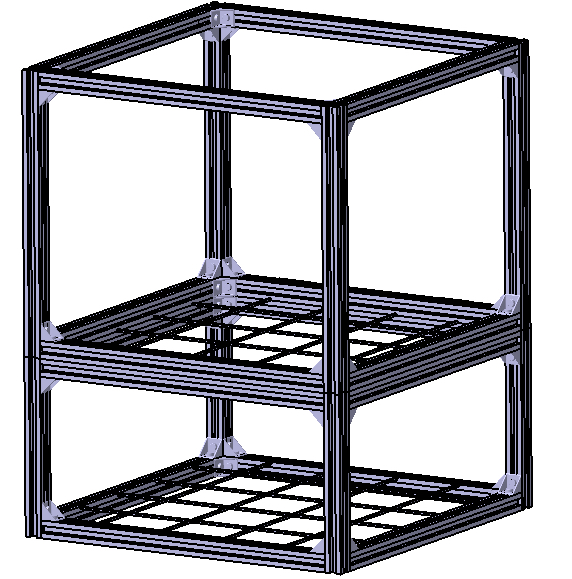
\includegraphics[width=0.7\textwidth, angle=90]{4-experiment-design/img/frame_structure.jpg}
%    \caption{Structure of the two-box design.}
%    \label{strucutre}
%\end{figure}



\DIFdelbegin %DIFDELCMD < \begin{figure}[!ht]
%DIFDELCMD <     \centering
%DIFDELCMD <     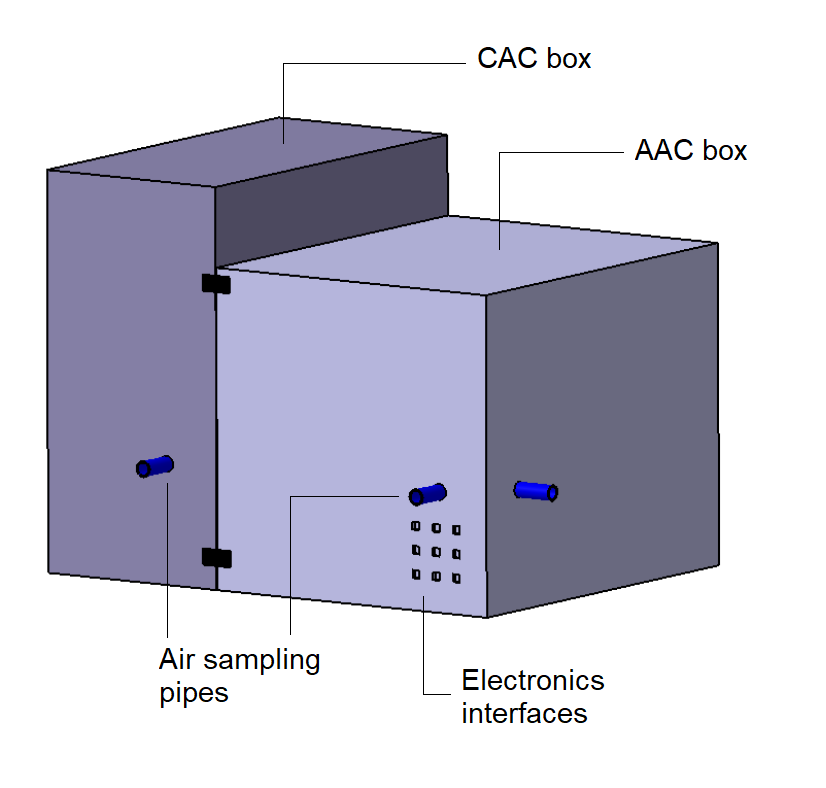
\includegraphics[width=0.7\textwidth]{4-experiment-design/img/overview_names.png}
%DIFDELCMD <     %%%
%DIFDELCMD < \caption{%
{%DIFAUXCMD
\DIFdelFL{General configuration of the experiment.}}
    %DIFAUXCMD
%DIFDELCMD < \label{overview}
%DIFDELCMD < \end{figure}
%DIFDELCMD < 

%DIFDELCMD < %%%
\DIFdelend \DIFaddbegin \pagebreak
\DIFaddend \subsubsection{CAC Subsystem}

The CAC subsystem is designed to fit a \DIFdelbegin \DIFdel{300-meter }\DIFdelend \DIFaddbegin \DIFadd{300 m stainless steel }\DIFaddend coiled tube, \DIFdelbegin \DIFdel{the }\DIFdelend \DIFaddbegin \DIFadd{a solenoid }\DIFaddend valve governing it\DIFdelbegin \DIFdel{and a temperature sensor. To determine its positioning }\DIFdelend \DIFaddbegin \DIFadd{, interfaces, an air filter and three temperature sensors. A schematic of this subsystem can be seen in Figure \ref{fig:CAC-schematic}. The CAC consists in a combination of a 200 m coiled tube of 1/8 in. and a 100 m coiled tube of 1/4 in. The outlet of the CAC is sealed with a quick connector provided by FMI. The inlet will be sealed in the same way but it will be open by means of another interfaced plugged to the quick connector. A filter is placed between this orifice and the solenoid valve. The filter will be custom made by FMI. The set up is a tube containing magnesium perchlorate powder with stone wool at both ends of the tube. It will ensure that no moisture will enter the coil during any testing or sampling. Another tube is attached to the solenoid valve that goes outside the box, thus having a direct outside outlet and inlet for the whole CAC system, as seen in Figure \ref{fig:CAC-cad-model}.
}

\smallskip
\DIFadd{The electronic components in the CAC box will be: three temperature sensors and the solenoid valve. In order to connect to these components, a male D-sub connector will be placed at a position on the wall of the box, where it is shortest distance to the EB in the AAC box (third level of The Brain). A female D-sub connector will also be placed on that wall of the AAC box. The connection between these plugs is made through a D-Sub wire. 
%DIF >  mechanical issues and gondola constraints 
}

\begin{figure}[H]
    \centering
    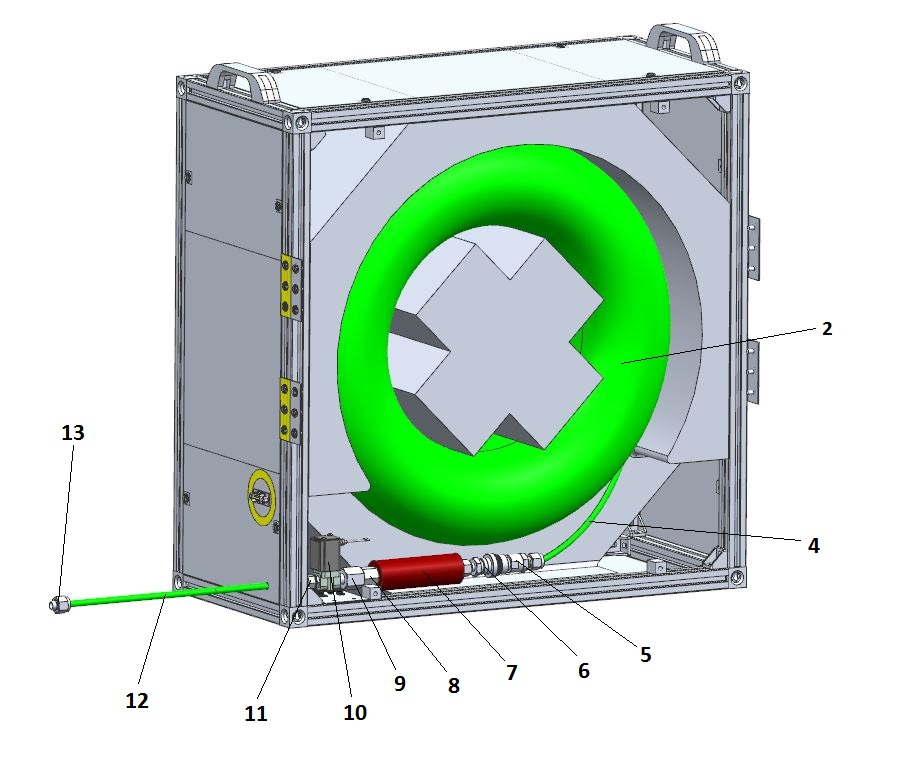
\includegraphics[width=0.8\textwidth]{4-experiment-design/img/Mechanical/CAC_interior_labels.jpg}
    \caption{\DIFaddFL{3D Model of the CAC Box. The Numbers Correspond to the Numbers in Figure \ref{fig:CAC-schematic}.}}
    \label{fig:CAC-cad-model}
\end{figure}

\begin{figure}[H]
    \centering
    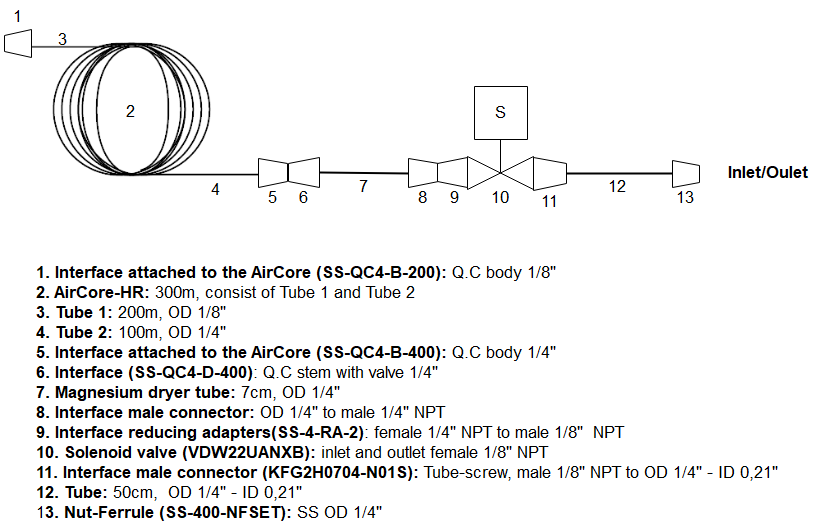
\includegraphics[width=1\textwidth]{4-experiment-design/img/CAC-schematic-v3.PNG}
    \caption{\DIFaddFL{Schematic of CAC}}
    \label{fig:CAC-schematic}
\end{figure}

\DIFadd{Since the CAC will be the heaviest component in the whole experiment, its positioning and orientation }\DIFaddend inside the gondola \DIFdelbegin \DIFdel{and the experiment box, some mechanical issues and gondola constraints }\DIFdelend \DIFaddbegin \DIFadd{will directly affect the stress analysis of the structure, hence it }\DIFaddend must be considered.

\smallskip
Firstly, it is possible to identify the interface to attach the experiment box to the gondola as one of the most critical points in terms of mechanics performance. In the worst case scenario, with a heavy experiment and without a proper study of the aforesaid interface, shear in the screws could be produced after a violent landing stress \DIFdelbegin \DIFdel{. Since the CAC will be the heaviest component in the whole experiment, its location and orientation will affect directly the stress analysis of the structure. }\DIFdelend \DIFaddbegin \DIFadd{or unexpected shaking. }\DIFaddend The larger the distance to the fixed points, the bigger the momentum produced by the component. Nevertheless, due to fast recovery implementation, the CAC tube will be placed vertically. Therefore, its dedicated box will be properly attached to the AAC box by means of \DIFdelbegin \DIFdel{4 }\DIFdelend \DIFaddbegin \DIFadd{four }\DIFaddend anchor points, \DIFdelbegin \DIFdel{in black in Figure \ref{overview}}\DIFdelend \DIFaddbegin \DIFadd{fast recovery fixing interface as seen in yellow in Figure \ref{dimensions}}\DIFaddend . The fast recovery then will only imply unscrewing \DIFdelbegin \DIFdel{4 screws and disconnecting a wire}\DIFdelend \DIFaddbegin \DIFadd{12 screws and unplugging a D-Sub connector}\DIFaddend . 


\DIFdelbegin %DIFDELCMD < \smallskip
%DIFDELCMD < %%%
\DIFdel{In order to command the valve, a wire will go out from the box and connected to the electronics interface panel located on an AAC box wall.
}%DIFDELCMD < 

%DIFDELCMD < \smallskip
%DIFDELCMD < %%%
\DIFdel{In addition, to avoid sample contamination with standstill air inside the gondola, the coil will have a direct outside inlet and outlet by means of an extension tube reaching further from the gondola’s limits, in blue in the red box in Figure \ref{overview}.
}%DIFDELCMD < 

%DIFDELCMD < %%%
\DIFdelend \DIFaddbegin \pagebreak
\DIFaddend \subsubsection{AAC Subsystem}\DIFaddbegin \label{sec:aac-analysis}
\DIFaddend 

The AAC Subsystem consists of \DIFdelbegin \DIFdel{10 three-liter }\DIFdelend \DIFaddbegin \DIFadd{six 3 L }\DIFaddend sampling bags. Each bag will have a dedicated valve in the Valve Center (VC) to allow emptying and filling processes as well as to close the bag when needed. The bags will be placed vertically and will have two anchor points: on the top through a  multiple anchor interface (see Figure \ref{anchor_bags}) and on the bottom by means of the tubes connecting them to the valves.

%% Several Figures of the top box with its inside elements: isometric, top view and front view.

\DIFdelbegin %DIFDELCMD < \begin{figure}[!ht]
%DIFDELCMD <     %%%
\DIFdelendFL \DIFaddbeginFL \begin{figure}[H]
    \DIFaddendFL \centering
    \DIFdelbeginFL %DIFDELCMD < 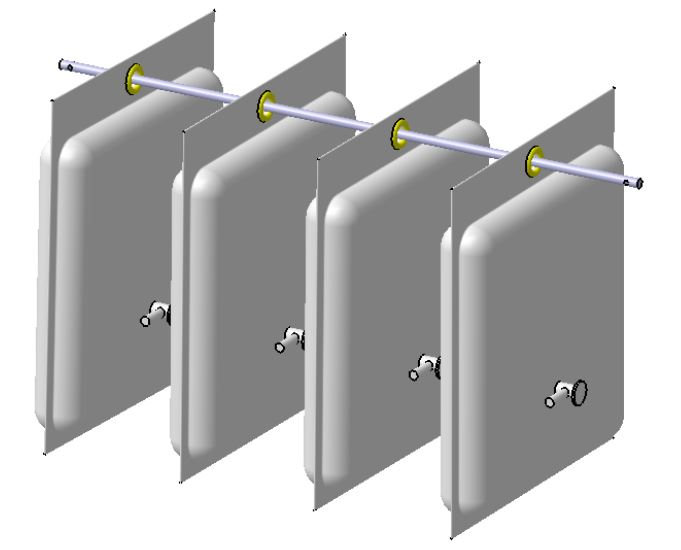
\includegraphics[width=0.7\textwidth]{4-experiment-design/img/bags_assembly.jpg}
%DIFDELCMD <     %%%
\DIFdelendFL \DIFaddbeginFL 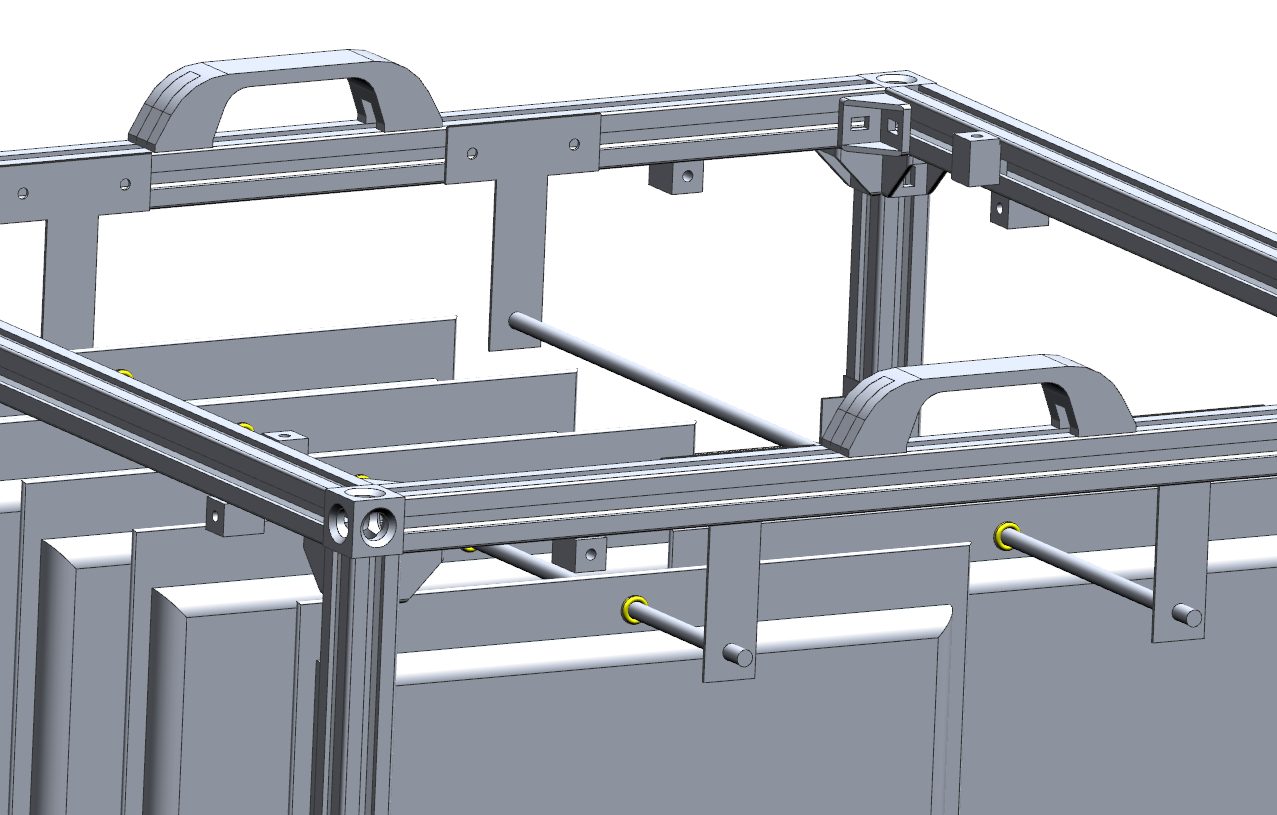
\includegraphics[width=0.7\textwidth]{4-experiment-design/img/Mechanical/Bags_Fixing_Interface.png}
    \DIFaddendFL \caption{Sampling \DIFdelbeginFL \DIFdelFL{bags }\DIFdelendFL \DIFaddbeginFL \DIFaddFL{Bags }\DIFaddendFL with \DIFdelbeginFL \DIFdelFL{fixing interface}\DIFdelendFL \DIFaddbeginFL \DIFaddFL{Fixing Interface and the AAC Box Handles}\DIFaddendFL .}
    \label{anchor_bags}
\end{figure}

\DIFdelbegin \subsubsection{\DIFdel{Electronics Box}}
%DIFAUXCMD
\addtocounter{subsubsection}{-1}%DIFAUXCMD
\DIFdelend \DIFaddbegin \DIFadd{Table \ref{table:bags-dimensions} shows how the dimensions of the bags change according to the sampled volume. This data has been obtained by testing and has been taken into account in order to determine the maximum number of bags that can be filled inside the box.
}\DIFaddend 

\DIFdelbegin \DIFdel{The OBC and its external elements will be allocated in a bottom }\DIFdelend \DIFaddbegin \begin{table}[H]
\noindent\DIFaddFL{\makebox[\columnwidth]{%
\scalebox{0.8}{
\begin{tabular}{|c|c|c|c|}
\hline
\textbf{Volume} & \textbf{Length (horizontal)}& \textbf{Height (vertical)} & \textbf{Width }\\ \hline
Empty & 26.4 cm & 28 cm & 0.5 cm \\ \hline
0.5 L & 26.4 cm & 27.5 cm & 1.5 cm \\ \hline
1 L & 26 cm & 27.5 cm & 2 cm \\ \hline
1.5 L & 25.5 cm & 26.5 cm & 4.5 cm \\ \hline
2 L & 25 cm & 25 cm & 5.5 cm \\ \hline
2.5 L & 24.5 cm & 23 cm & 7.5 cm \\ \hline
3 L & 24 cm & 22 cm & 10.5 cm \\ \hline
\end{tabular}}}
}\caption{\DIFaddFL{Dimensions of the Bags When Filled with Different Air Sample Volumes}}
\label{table:bags-dimensions}
\end{table}

\pagebreak
\underline{\DIFadd{Distribution}}

\DIFadd{The AAC box has been designed in order to be as compact as possible. Nonetheless, the latter was a challenging iterative process since the bags dimensions vary during the flight. The process led to a square base box that is able to fit six sampling bags together with a control center called The Brain that includes the pneumatic system and the electronic box. The distribution layout can be seen in Figures \ref{iso_aac} and \ref{lateral_aac}.
}

%DIF >  Figure: Top view to show the distribution of the AAC Box

\begin{figure}[H]
    \centering
    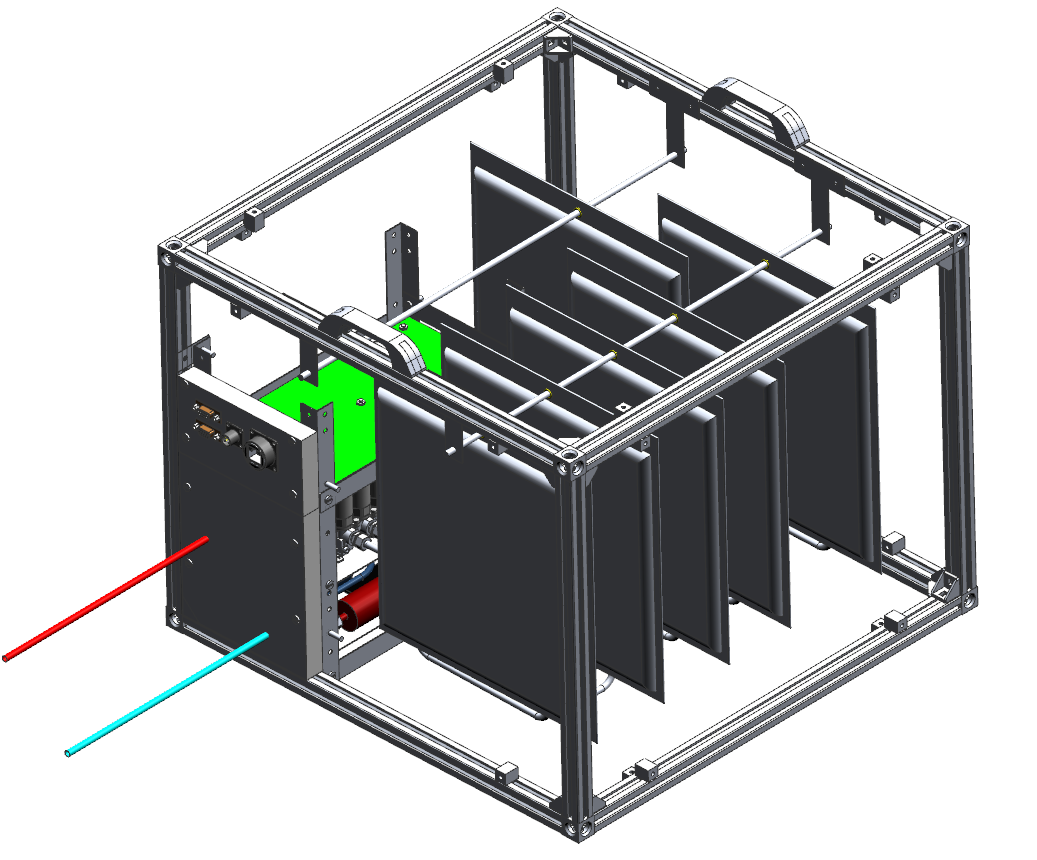
\includegraphics[width=0.8\textwidth]{4-experiment-design/img/Mechanical/AAC_isometric_view.png}
    \caption{\DIFaddFL{Isometric View of the AAC Box.}}
    \label{iso_aac}
\end{figure}


\begin{figure}[H]
    \centering
    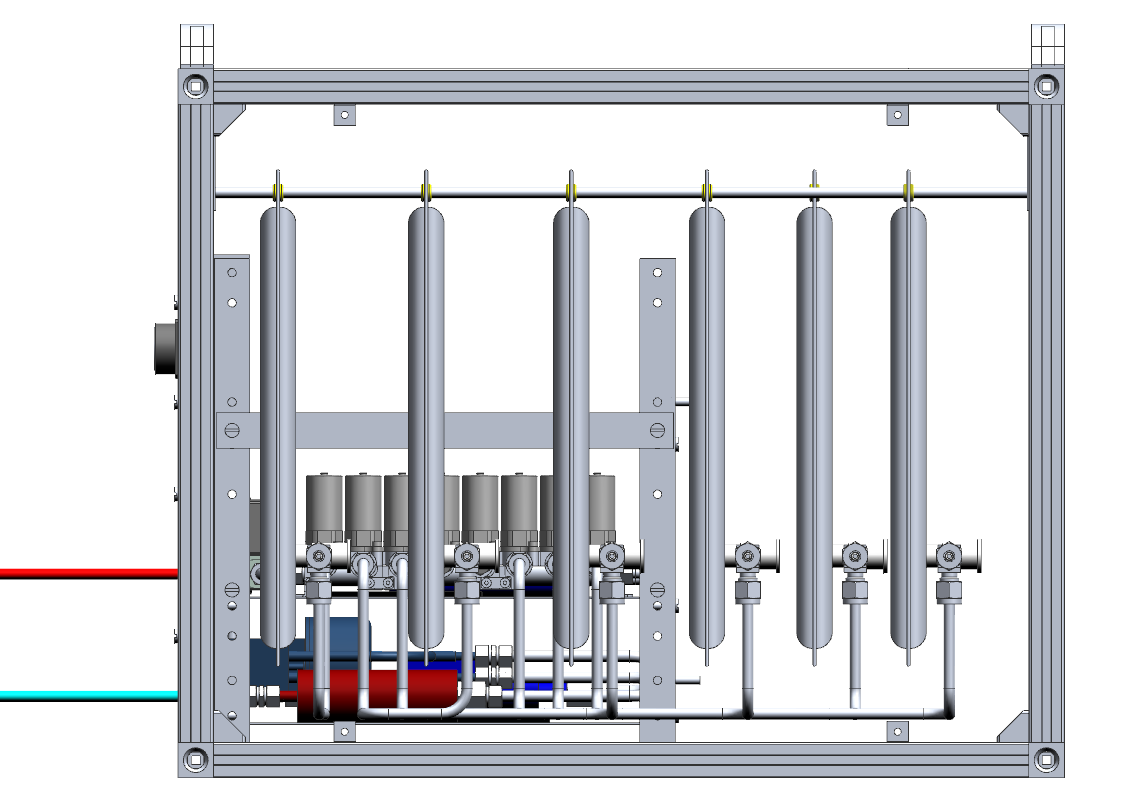
\includegraphics[width=0.8\textwidth]{4-experiment-design/img/Mechanical/AAC_lateral_view.png}
    \caption{\DIFaddFL{Lateral View of the AAC Box.}}
    \label{lateral_aac}
\end{figure}

\begin{figure}[H]
    \centering
    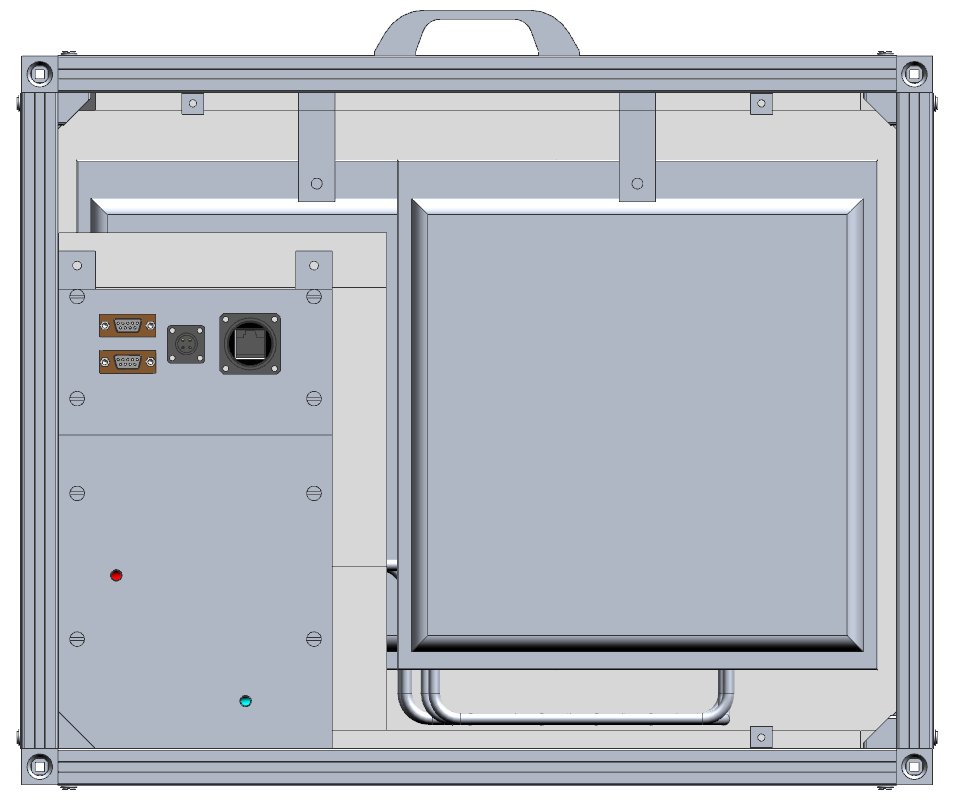
\includegraphics[width=0.8\textwidth]{4-experiment-design/img/Mechanical/AAC_front_view.png}
    \caption{\DIFaddFL{Front View of the AAC Box.}}
    \label{front_aac}
\end{figure}

\DIFadd{In order to reach to all the bags from the Valve Center, the tubes are brought to the base of the box. More detail on its positioning is included in the following section. 
}

\smallskip
\DIFadd{Since the AAC box is expected to be handed over to FMI, the design also takes into consideration the possibility to include a battery for power supply. This would be allocated next to the Brain. The latter would imply reducing the sampling bags down to five, see Figure \ref{battery_distribution}.
}

%DIF >  Figure with a a top view without the 6th bag and with a red box simulating the battery

\begin{figure}[H]
    \centering
    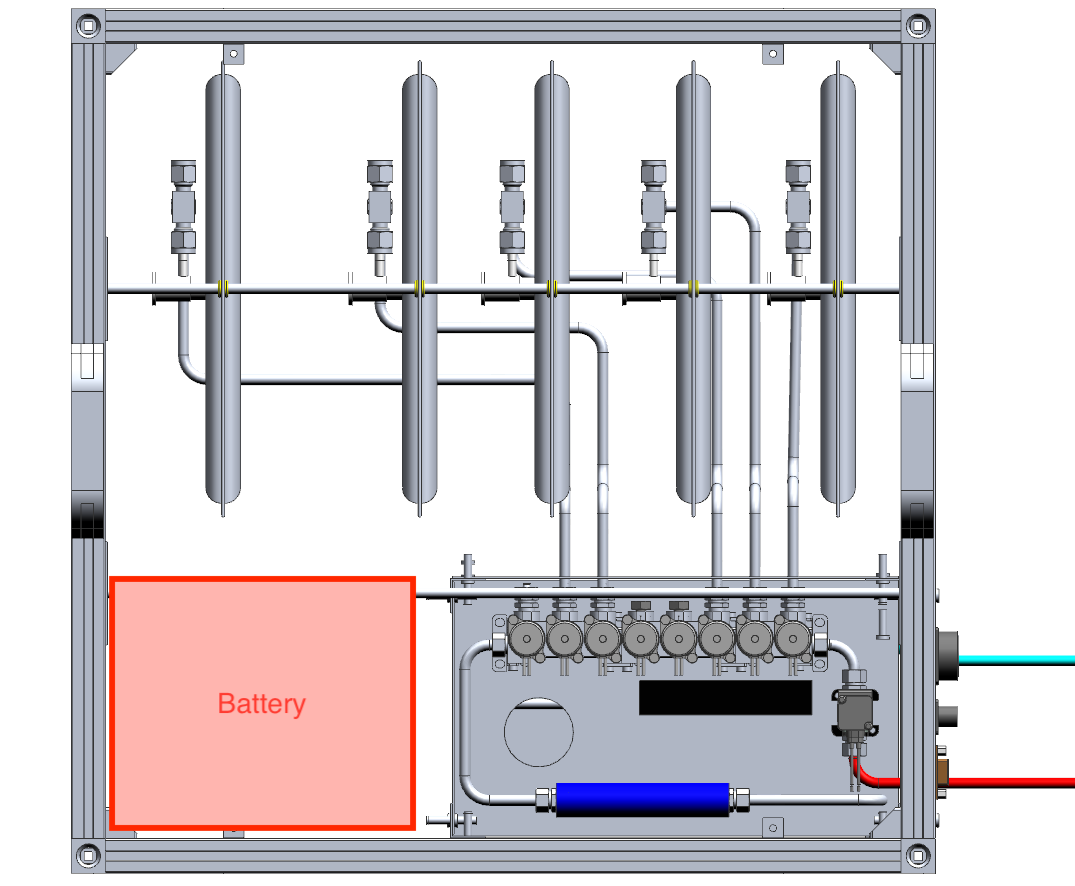
\includegraphics[width=0.8\textwidth]{4-experiment-design/img/Mechanical/Battery_Top_View.png}
    \caption{\DIFaddFL{Layout Including a Battery (in red)}}
    \label{battery_distribution}
\end{figure}


\pagebreak
\subsubsection{\DIFadd{The Brain}}

\DIFadd{The control unit, so called The Brain, is an essential part of the experiment. It is a three-level structure containing both the pneumatic system and the electronics of the experiment, seen in Figure \ref{brain_isometric_open}. Its design aimed to make it compact enough for both allow a proper thermal control and to fit into the space left next to the sampling bags. It is placed in a }\DIFaddend corner of the \DIFdelbegin \DIFdel{experiment box, inside AAC box, and on the opposite side of the CAC box }\DIFdelend \DIFaddbegin \DIFadd{AAC box}\DIFaddend . 
\DIFdelbegin \DIFdel{This will allow an easy access and manipulation }\DIFdelend \DIFaddbegin 

\DIFadd{Therefore, the Brain takes advantage of the vertical space inside the AAC box. It has three different levels: 
}

\begin{itemize}
    \item \DIFadd{Level 1: Pump
    }\item \DIFadd{Level 2: Valve Center
    }\item \DIFadd{Level 3: Electronics
}\end{itemize}


\begin{figure}[H]
    \centering
    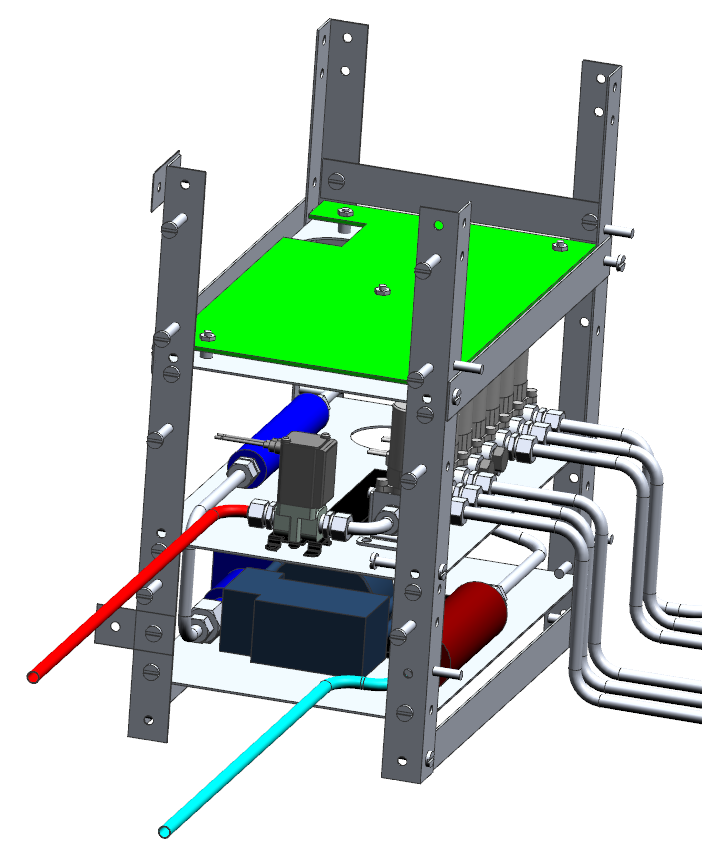
\includegraphics[width=0.8\textwidth]{4-experiment-design/img/Mechanical/Brain_Isometric_Open.png}
    \caption{\DIFaddFL{Isometric View of The Brain without walls.}}
    \label{brain_isometric_open}
\end{figure}

\DIFadd{Level 1 is the base of the AAC box and together with Level 2 contain the main pneumatic system. This is commanded by the electronics in the top level. This distribution allows easy access to the PCB from the top and provides the physical desired separation between electronics and pneumatic circuit. 
}

\DIFadd{The fact of having different levels implies the need of having dedicated holes to bring all the wires to the third level and the tube to the second level. This is shown in the dedicated section for each level which can be seen in Figure \ref{brain_lateral}.
}

\begin{figure}[H]
    \centering
    \includegraphics[width=0.8\textwidth]{4-experiment-design/img/Mechanical/Brain_Lateral.png}
    \caption{\DIFaddFL{Lateral View of The Brain.}}
    \label{brain_lateral}
\end{figure}

\smallskip
\DIFadd{The structure of the Brain provides versatility in terms of implementation and construction. It is made out of four aluminum 90-degree angle bars and five flat bars to join them together. The bars have custom-made holes that allow the 1 mm thick aluminum plate of each level to be fixed by means of two bolts on each column, one over and one below it. They allow the possibility to provide the anchor point for the lateral and top styrofoam shield }\DIFaddend as well as \DIFdelbegin \DIFdel{the required external interfaces, holes in Figure \ref{overview}.
The smallest side of the EB will have the outer connectionsinterfaces. Hence, the wall will have the necessary holes. The EB will be fixed to the AAC box structure bars in }\DIFdelend \DIFaddbegin \DIFadd{to fix the whole unit to the box structure bars. This is seen in Figure \ref{brain_structure}. 
}

\begin{figure}[H]
    \centering
    \includegraphics[width=0.8\textwidth]{4-experiment-design/img/Mechanical/Brain_Structure.png}
    \caption{\DIFaddFL{Structure of The Brain.}}
    \label{brain_structure}
\end{figure}

\smallskip
\DIFadd{The bulk dimensions of the brain are 260 mm long, 150mm wide and 290 mm high. If the shielding styrofoam walls are taken into account, the dimensions are 290 mm long, 180 mm wide and 300 mm high.
Therefore, accounting for the space the column bars take, each plate has a surface of 258 mm x 158 mm. The distance between levels is variable depending on the components dimensions. Level 1 has a height if 7 cm, Level 2 has a height of 9cm and Level }\DIFaddend 3 \DIFdelbegin \DIFdel{different points. }\DIFdelend \DIFaddbegin \DIFadd{has 8cm to the top styrofoam shielding. The Brain with styrofoam sheilding can be seen in Figure \ref{brain_isometric}.
}\DIFaddend 

%DIF < % Figure of the electronics box inside the coil, only bottom cube, isometric top view, explosion
\DIFaddbegin \begin{figure}[H]
    \centering
    \includegraphics[width=0.8\textwidth]{4-experiment-design/img/Mechanical/Brain_Isometric.png}
    \caption{\DIFaddFL{Isometric View of the Brain.}}
    \label{brain_isometric}
\end{figure}
\DIFaddend 

%DIF < \begin{figure}[!ht]
 %DIF <    \centering
  %DIF <   \includegraphics[width=0.7\textwidth]{4-experiment-design/img/explos_CAC.jpg}
   %DIF <  \caption{.}
    %DIF < \label{electronics_box}
%DIF < \end{figure}
\DIFaddbegin \smallskip
\DIFadd{In order to allocate the electrical interfaces required (E-Link, Power Supply and D-Sub Connectors) as well as to allow the tubes of the sampling system to reach the outside environment, the outside facing wall is divided in three pieces. Two small pieces are fixed to the Brain structure. The latter provides easiness of manipulation when having to open the box wall since the little pieces containing the interfaces and the tubes holes, will remain attached. The bottom piece covers Level 1 and 2 while the other, which contains the electrical connections, protects Level 3. These pieces have the same layout as the main wall. 
}\DIFaddend 


\pagebreak
\DIFdelbegin \subsubsection{\DIFdel{Valve Center}}
%DIFAUXCMD
\addtocounter{subsubsection}{-1}%DIFAUXCMD
\DIFdelend \DIFaddbegin \underline{\DIFadd{Level 1 - Pump}}
\DIFaddend 

\DIFdelbegin \DIFdel{The valve center consists of a coated box to which the AAC's 10 air sampling bags will be attached to. This box will serve as airflow chamber. 
It will be connected to a pipe from which outside air will be pumped and also enable pre-sample collection flushing.
The pump providing the airflow }\DIFdelend \DIFaddbegin \smallskip
\DIFadd{List of components of Level 1:
}

\begin{enumerate}[label=\Alph*.]
    \item \DIFadd{1 Magnesium filter (M48)
    }\item \DIFadd{1 Pump (E3)
    }\item \DIFadd{1 Airflow sensor (E6)
    }\item \DIFadd{1 Temperature sensor (E9)
    }\item \DIFadd{2 Heaters (E7)
    }\item \DIFadd{4 Tubes (M45)
    }\item \DIFadd{3 Straight union interfaces (M41)
    }\item \DIFadd{3 Female to tube interfaces (M42)
}\end{enumerate}


\begin{figure}[H]
    \centering
    \includegraphics[width=0.8\textwidth]{4-experiment-design/img/Mechanical/Level_1.png}
    \caption{\DIFaddFL{Isometric View of Level 1.}}
    \label{level_1}
\end{figure}

\smallskip
\DIFadd{The bottom level of The Brain is lying on the base wall styrofoam. It contains the beginning of the pneumatic sampling system. The inlet tube passes through the panel wall and interfaces with the filter. From here the system continues through the pump, airflow sensor and to Level 2.
The reason for having the pump in Level 1 is to have the minimum vibration transmitted to the other components. The pump will have two heaters close by that will be used to regulate its temperature. This can be seen in Figure \ref{level_1}
}


\pagebreak
\underline{\DIFadd{Level 2 - Valve Center}}


\DIFadd{List of components of Level 2:
}

\begin{enumerate}[label=\Alph*.]
    \item \DIFadd{1 Sensor Box (M49)
    }\item \DIFadd{3 Pressure sensors (E4)
    }\item \DIFadd{1 Humidity sensor (E11)
    }\item \DIFadd{1 Temperature sensor (E9)
    }\item \DIFadd{1 Heater (E7)
    }\item \DIFadd{1 Manifold (M50)
    }\item \DIFadd{8 Sampling valves (E36)
    }\item \DIFadd{1 Flushing valve (E37)
    }\item \DIFadd{12 Male to tube interfaces (M40)
    }\item \DIFadd{2 Caps (M47)
    }\item \DIFadd{12 Tubes (M45)
}\end{enumerate}


\begin{figure}[H]
    \centering
    \includegraphics[width=0.8\textwidth]{4-experiment-design/img/Mechanical/Level_2.png}
    \caption{\DIFaddFL{Isometric View of Level 2.}}
    \label{level_2}
\end{figure}

\smallskip
\DIFadd{This level of the Brain is responsible of the distribution of the air to the selected sampling bag. The manifold with 8 solenoid valves is the main component. From here, the tubes connect with the bags. A T-Union connection is used just before the bag valve. This interface allows the pre-flight flushing of the tubes connecting with the valves as explained previously. 
}

\smallskip
\DIFadd{The flushing valve is the responsible to ensure a proper flushing of the system before each sampling period. From the flushing valve, a the outlet tube (in red) reaches the outside environment. This can be seen in Figure \ref{level_2}.
}



\pagebreak
\underline{\DIFadd{Level 3 - Electronics}}


\DIFadd{List of components of Level 3:
}\begin{enumerate}[label=\Alph*.]
    \item \DIFadd{1 PCB
    }\item \DIFadd{2 D-Sub female connectors (E23)
    }\item \DIFadd{1 E-link socket (E35)
    }\item \DIFadd{1 Power socket (E33)
}\end{enumerate}


\begin{figure}[H]
    \centering
    \includegraphics[width=0.8\textwidth]{4-experiment-design/img/Mechanical/Level_3.png}
    \caption{\DIFaddFL{Isometric View of Level 3.}}
    \label{level_3}
\end{figure}

\smallskip
\DIFadd{The OBC and its external elements }\DIFaddend will be allocated \DIFdelbegin \DIFdel{on the inlet side and protected by an air filter. It will be allocated inside a shielding box}\DIFdelend \DIFaddbegin \DIFadd{in the third level of the Brain. The PCB will be fixed to the aluminum plate by means of 5 standoffs. As shown in Figure \ref{level_3}, it has a hole, as well as the level plate, to collect all the wires connecting with levels 1 and 2. This level has its own outside wall which contains the electrical interfaces. The latter allows to open the wall without having to remove all the sockets attached with screws and a female in the inside of the wall. The styrofoam shielding the Brain has a hole at this height to allow the temperature sensors wires to reach the inside of the AAC Box. All the electrical components connected to the PCB in Level 3 are summarized in Tables \ref{tab:list_of_components_CAC} and \ref{tab:list_of_components_AAC}.
}

\begin{table}[H]
\centering

\begin{tabular}{|l|l|l|}
\hline
\multicolumn{3}{|c|}{\textbf{CAC}}                                                                                      \\ \hline
\multicolumn{1}{|c|}{Area}                        & \multicolumn{1}{c|}{Electrical component} & \multicolumn{1}{c|}{\#} \\ \hline
\rowcolor[HTML]{FFCC67} 
\cellcolor[HTML]{FFCC67}                          & \DIFaddFL{Solenoid valve                            }& \DIFaddFL{1                       }\\ \cline{2-3} 
\rowcolor[HTML]{FFCC67} 
\multirow{-2}{*}{\cellcolor[HTML]{FFCC67}CAC} & \DIFaddFL{Temperature sensor                        }& \DIFaddFL{3                       }\\ \hline
\end{tabular}
\caption{\DIFaddFL{Connections to CAC Box}}
\label{tab:list_of_components_CAC}
\end{table}
\begin{table}[H]
\centering
\begin{tabular}{|l|l|l|}
\hline
\multicolumn{3}{|c|}{\textbf{AAC}}                                                  \\ \hline
\multicolumn{1}{|c|}{Area}                             & \DIFaddFL{Electrical component }& \DIFaddFL{\# }\\ \hline
\rowcolor[HTML]{FFCCC9} 
\cellcolor[HTML]{FFCCC9}                               & \DIFaddFL{Pump                  }& \DIFaddFL{1  }\\ \cline{2-3} 
\rowcolor[HTML]{FFCCC9} 
\cellcolor[HTML]{FFCCC9}                               & \DIFaddFL{Heater                }& \DIFaddFL{2  }\\ \cline{2-3} 
\rowcolor[HTML]{FFCCC9} 
\cellcolor[HTML]{FFCCC9}                               & \DIFaddFL{Airflow sensor        }& \DIFaddFL{1  }\\ \cline{2-3} 
\rowcolor[HTML]{FFCCC9} 
\multirow{-4}{*}{\cellcolor[HTML]{FFCCC9}Level 1}     & \DIFaddFL{Temperature sensor    }& \DIFaddFL{1  }\\ \hline
\rowcolor[HTML]{9AFF99} 
\cellcolor[HTML]{9AFF99}                               & \DIFaddFL{Humidity sensor       }& \DIFaddFL{1  }\\ \cline{2-3} 
\rowcolor[HTML]{9AFF99} 
\cellcolor[HTML]{9AFF99}     & \DIFaddFL{Pressure sensor       }& \DIFaddFL{3  }\\ 
   \cline{2-3} 
\rowcolor[HTML]{9AFF99} 
\cellcolor[HTML]{9AFF99}                               & \DIFaddFL{Solenoid valves       }& \DIFaddFL{9  }\\ \cline{2-3} 
\rowcolor[HTML]{9AFF99} 
\cellcolor[HTML]{9AFF99}                               & \DIFaddFL{Heater                }& \DIFaddFL{1  }\\ \cline{2-3} 
\rowcolor[HTML]{9AFF99} 
\multirow{-5}{*}{\cellcolor[HTML]{9AFF99}Level 2}  & \DIFaddFL{Temperature sensor    }& \DIFaddFL{1  }\\ \hline
\rowcolor[HTML]{96FFFB} 
\DIFaddFL{Sampling bags center                                         }& \DIFaddFL{Temperature sensor    }& \DIFaddFL{3  }\\ \hline
\end{tabular}
\caption{\DIFaddFL{Connections to AAC System}}
\label{tab:list_of_components_AAC}
\end{table}


\pagebreak
\underline{\DIFadd{Shielding and anchor points}}

\DIFadd{The most critical components in terms of required thermal control are inside the Brain. These are the pump (E3) and the valves (E36 and E37). In order to provide a passive thermal shielding}\DIFaddend , \DIFdelbegin \DIFdel{more detailed information in section \ref{Thermal_section}. The pipes used for both intake and outlet }\DIFdelend \DIFaddbegin \DIFadd{3cm thick removable styrofoam walls are placed in the three walls (top and laterals) facing the interior of the AAC box, see Figure \ref{brain_front}. The lateral walls are fixed by means of four bolts attached to the structure bars that penetrate inside the styrofoam. The top wall is fixed in place taking advantage of the structure columns which penetrate inside it. The larger lateral wall, where the tubes from the valves are, is divided in two pieces so it can be removed without having to disconnect the tubes. 
}

\smallskip
\DIFadd{The Brain is fixed to the structure of the AAC box by means of two anchor points. In order to keep it in its place, the structure bars penetrate 3 cm into the styrofoam base.
}

\begin{figure}[H]
    \centering
    \includegraphics[width=1\textwidth]{4-experiment-design/img/Mechanical/Panel_Front.png}
    \caption{\DIFaddFL{Front View of the Brain Where the Styrofoam Walls can be Identified.}}
    \label{brain_front}
\end{figure}


\pagebreak
\subsubsection{\DIFadd{Pneumatic System}}
\label{sec:4.4.5}

\DIFadd{In order to be able to collect separated samples of air, a pneumatic system has been developed. The schematics and components of this }\DIFaddend can be seen in \DIFdelbegin \DIFdel{blue in the grey box in Figure \ref{overview}. }\DIFdelend \DIFaddbegin \DIFadd{Figure \ref{pneumatic_system} . The circuit is formed by a total of 81 components located inside the Brain and the AAC Box. 
}\DIFaddend 


\DIFdelbegin %DIFDELCMD < \smallskip
%DIFDELCMD < %%%
\DIFdel{Both the pump box and }\DIFdelend \DIFaddbegin \DIFadd{The schematic for the pneumatic system can be seen in Figure \ref{pneumatic_system}. The air is sucked from the outside through the inlet tube (No.1), turquoise in Figure \ref{level_1_pneumatic_system_top_view}, and it goes through the filter (No.3) inside the pump (No.7). From here, it passes through the airflow sensor (No.11), which allows to monitor the flow rate, before changing to Level 2 (Figure \ref{level_2_pneumatic_system_top_view}). There, the sensor box (No.15) containing three pressure sensors and one humidity sensor, is the first component the air passes through before getting to the 8 stations manifold (No.19). It is in here where the air is directed to the desired bag (No.31) thanks to its dedicated solenoid valve (No.26). 
When flushing the circuitry before each sampling period, the flushing valve (No.23) is opened so }\DIFaddend the \DIFdelbegin \DIFdel{valve center will be allocated above the EB so all the command center is at the same place. 
Having them together will provide as well a proper cooling system monitored by several temperature sensors. %DIF < A sketch of the setup can be seen in Figure ....
}\DIFdelend \DIFaddbegin \DIFadd{outlet of the system is opened so new air runs through the main circuit. 
}\DIFaddend 

%DIF < % Figure of the valve center with the pipe and small tubes
\DIFaddbegin \begin{figure}[H]
    \centering
    \includegraphics[width=0.8\textwidth]{4-experiment-design/img/Mechanical/Pneumatic_System_Top_View_Level_1.png}
    \caption{\DIFaddFL{Pneumatic System top View of Level 1.}}
    \label{level_1_pneumatic_system_top_view}
\end{figure}
\DIFaddend 

%DIF < \begin{figure}[!ht]
%DIF <     \centering
%DIF <     \includegraphics[width=0.9\textwidth]{4-experiment-design/img/valve_collector.jpg}
%DIF <     \caption{Valve center with all the tubes to the sampling bags and to the outside environment.}
%DIF <     \label{valve_center_and_pipes}
%DIF < \end{figure}
\DIFaddbegin \begin{figure}[H]
    \centering
    \includegraphics[width=0.8\textwidth]{4-experiment-design/img/Mechanical/Pneumatic_System_Top_View_Level_2.png}
    \caption{\DIFaddFL{Pneumatic System top View of Level 2.}}
    \label{level_2_pneumatic_system_top_view}
\end{figure}
\DIFaddend 

%DIF < % Add figure with EB and external interface + VC + Pump Box + Pipes + fixing elements
%DIF >  Figure with the diagram

\DIFaddbegin \newpage
\begin{landscape}
\begin{figure}[H]
    \centering
    \includegraphics[width=1.5\textwidth]{4-experiment-design/img/Mechanical/AAC_Subsystem.png}
    \caption{\DIFaddFL{AAC Pneumatic System Diagram and Components.}}
    \label{pneumatic_system}
\end{figure}
\end{landscape}


\pagebreak
\DIFaddend \subsubsection{Protection}

In order to protect the components from all kind of external elements, the experiment box will be shielded with removable aluminum walls along with a thick layer of Styrofoam \DIFdelbegin \DIFdel{combined with Polyethylene foam }\DIFdelend attached to each wall. No internal space will be lost since the total foam thickness is the same as that of the structural bars \DIFdelbegin \DIFdel{. Isolating sheets will also be glued in the walls to reinforce the temperature shielding}\DIFdelend \DIFaddbegin \DIFadd{in the majority of the walls}\DIFaddend . 


The walls will \DIFdelbegin \DIFdel{properly }\DIFdelend protect both the CAC coiled tube and the AAC sampling bags from any external element, unexpected rapid movements, and a probable hard landing impact. %see in Figure \ref{walls}. 
\DIFdelbegin %DIFDELCMD < 

%DIFDELCMD < %%%
%DIF < % Cut: Figure CAC+EB, AAC+valve center, and walls + Styrofoam. Label all the parts
%DIFDELCMD < 

%DIFDELCMD < %%%
%DIF < \begin{figure}[!ht]
%DIF <     \centering
%DIF <     \includegraphics[width=0.2\textwidth]{4-experiment-design/img/tall_frontal.jpg}
%DIF <     \caption{Wall layers.}
%DIF <     \label{walls}
%DIF < \end{figure}
%DIFDELCMD < 

%DIFDELCMD < %%%
\DIFdel{The front walls, face of the experiment box exposed to the outside, will have several holes: to allow the tubes providing air flow to collect clean air from the outside, and to manipulate the electric connections.
}%DIFDELCMD < 

%DIFDELCMD < %%%
%DIF < The top lateral walls will have four holes to allow the introduction of the circular bars used as anchor points for the sampling bags, see Figure \ref{anchor_bags}.
%DIFDELCMD < 

%DIFDELCMD < %%%
\DIFdelend Bolts shall be used to attach all walls to the structure's railed bars. \DIFaddbegin \DIFadd{See Section \ref{sec:4.2.1} for detail on fixing points.
}\DIFaddend 

%% Figure front wall holes: isometric Include labels

%\begin{figure}[!ht]
%    \centering
%    \includegraphics[width=0.7\textwidth]{4-experiment-design/img/frontal_holes.jpg}
%    \caption{External view of the experiment.}
%    \label{front_wall_holes}
%\end{figure}

\DIFdelbegin \subsubsection{\DIFdel{Fixing Interface}}
%DIFAUXCMD
\addtocounter{subsubsection}{-1}%DIFAUXCMD
%DIFDELCMD < 

%DIFDELCMD < %%%
\DIFdel{The two experiment box subsystem structures will be joined together by four anchor points, in black in Figure \ref{overview}. On the front and back side, two flat plates with two bolts each will interface both structures. 
}%DIFDELCMD < 

%DIFDELCMD < %%%
\DIFdel{This method will allow for easy and fast recovery of the CAC box. 
 }%DIFDELCMD < 

%DIFDELCMD < %%%
%DIF < % Figure with the two boxes attached
%DIFDELCMD < 

%DIFDELCMD < %%%
\subsubsection{\DIFdel{Manipulation Interface}}
%DIFAUXCMD
\addtocounter{subsubsection}{-1}%DIFAUXCMD
%DIFDELCMD < 

%DIFDELCMD < %%%
\DIFdel{The two-box system will be fixed to the gondola rails by using four 90-degree angles, 2 per rail. All the anchor points to the gondola will be in the AAC box since the CAC box will be already attached to it. The latter also ensures that the AAC box will remain properly fixed in the gondola after the CAC fast recovery.
    }%DIFDELCMD < 

%DIFDELCMD < \smallskip
%DIFDELCMD < %%%
\DIFdel{In order to access the experiment once fixed in the gondola, the walls could be removed when necessary providing access in all three directions.
    They can be screwed in again once the manipulation is done.
}%DIFDELCMD < 

%DIFDELCMD < %%%
\DIFdel{Several handles will be placed to allow an easy and safe manipulation of both the CAC and the AAC boxes.
    }%DIFDELCMD < 

%DIFDELCMD < %%%
\subsubsection{\DIFdel{Mechanical Components}}
%DIFAUXCMD
\addtocounter{subsubsection}{-1}%DIFAUXCMD
%DIFDELCMD < 

%DIFDELCMD < %%%
\DIFdel{All the components used in the mechanical design can be found in Table \ref{tab:mechanical-components}.
    Spare elements are not included.
}%DIFDELCMD < 

%DIFDELCMD < %%%
\DIFdelend \raggedbottom
\pagebreak
\subsection{Electrical Design}

\DIFdelbegin \subsubsection{\DIFdel{Block Diagrams}}
%DIFAUXCMD
\addtocounter{subsubsection}{-1}%DIFAUXCMD
%DIFDELCMD < \begin{centering}
%DIFDELCMD < %%%
\DIFdel{The electronics design can be seen in Figure \ref{fig:electronics-block-diagram} and the interfaces this requires can be seen in Figure \ref{fig:eee-interface-diagram}. There will be four distinct areas, the Electronics box, the valve centre, the pump box and the CAC system. All connections to the outside of the box are located in the electronics box. These are the voltage regulators for the external power source and the Ethernet shield with an SD data storage which will connect to the Telemetry, Tracking, and Command (TT\&C). Additionally one pressure sensor, one heater and one temperature sensor will be placed in this area.
The CAC system area will contain three temperature sensorsto monitor its ambient temperature and one electronic valve to be closed before landing. In the AAC system area there will be eleven valves, one airflow sensor, one pressure sensor, five temperature and one humidity sensor and a heater. In the pump box there will be the miniature diaphragm air pump, one temperature sensor and one heater. 
}%DIFDELCMD < \end{centering}
%DIFDELCMD < \bigskip
%DIFDELCMD < %%%
\DIFdelend \DIFaddbegin \subsubsection{\DIFadd{Block Diagram}}
\label{sec:4.5.1}

\DIFadd{The electronics design can be seen in Figure \ref{fig:electronics-block-diagram} which shows the connections, grounding, voltages, and signals. 
}\DIFaddend 

\begin{figure}[H]
    \DIFdelbeginFL \begin{align*}
        \DIFdelFL{\includegraphics[width=16cm]{4-experiment-design/img/block-diagram-four-sections.png}
    }\end{align*}
    %DIFAUXCMD
%DIFDELCMD < \caption{%
{%DIFAUXCMD
\DIFdelFL{Block Diagram for all Electronic Components Showing the Signal and Power Connections}}%DIFAUXCMD
\DIFdelendFL \DIFaddbeginFL \begin{align*}
        \DIFaddFL{\includegraphics[width=16cm]{block-diagram-2.png}
    }\end{align*}
    \caption{\DIFaddFL{Block Diagram for all Electronic Components Showing the Connection, Signal and Power Connections}}\DIFaddendFL \label{fig:electronics-block-diagram}
\end{figure}

\DIFdelbegin %DIFDELCMD < \begin{figure}[H]
%DIFDELCMD <     %%%
\begin{align*}
        \DIFdelFL{\includegraphics[width=16cm]{4-experiment-design/img/interface-diagram-electric.png}
    }\end{align*}
    %DIFAUXCMD
%DIFDELCMD < \caption{%
{%DIFAUXCMD
\DIFdelFL{Block Diagram Showing the Interfaces Between All Electrical Components.}}%DIFAUXCMD
%DIFDELCMD < \label{fig:eee-interface-diagram}
%DIFDELCMD < \end{figure}
%DIFDELCMD < %%%
\DIFdelend \DIFaddbegin \DIFadd{Most of the electronics will be located in the Brain inside the AAC box. However, there will be six distinct areas:
}\DIFaddend 

\DIFdelbegin %DIFDELCMD < \begin{centering}
%DIFDELCMD < %%%
\DIFdel{Three }\DIFdelend \DIFaddbegin \begin{enumerate}
    \item \DIFadd{The Brain level 3, where the PCB is located with the Arudino and shield, two 24 V }\DIFaddend DC-DC\DIFdelbegin \DIFdel{converters will be used to step down the voltage from the 28.8V provided by the gondola down to: 
}%DIFDELCMD < \end{centering}
%DIFDELCMD < %%%
\DIFdelend \DIFaddbegin \DIFadd{, one 12 V voltage regulator, one temperature sensor, 11 MOSFETs and 14 LEDs.
    }\item \DIFadd{The Brain level 2, where the valve manifolds with six sampling valves}\footnote{\DIFadd{There will be eight valves connected mechanically in the manifold to ensure it is sealed but only six will be connected to the bags and electronics.}\label{fn:extravalve}}\DIFadd{, the flushing valve, one heater and one temperature sensor are located.
    }\item \DIFadd{The Brain level 1, where the pump, airflow sensor and sensor box containing 3 pressure sensors, 1 temperature sensor and 1 humidity sensor are located.
    }\item \DIFadd{The AAC box, where 3 ambient temperature sensors are located.
    }\item \DIFadd{The CAC box, where the CAC valve and 3 ambient temperature sensors are located.
    }\item \DIFadd{Outside of the experiment box, where 3 ambient pressure sensors are located.
}\end{enumerate}
\DIFaddend 

\DIFdelbegin %DIFDELCMD < \begin{centering}
%DIFDELCMD < %%%
\DIFdelend \DIFaddbegin \DIFadd{From the PCB, on level 3, five D-sub connectors will be used to connect to the other five areas. A 25 pin connector will be used for level 1, 15 pin connector will be used for level 2 and nine pin connectors will be used for the CAC box, AAC box sampling bags area, and the external pressure sensors. In addition there will be a connection to the gondola power and gondola E-link.
}

\DIFadd{All of the power distribution will take place on the PCB using two 24 V DC-DC converters in parallel with a forwarding diode which feed a 12 V voltage regulator. 
}\DIFaddend \begin{itemize}
  \item \DIFdelbegin \DIFdel{\mbox{%DIFAUXCMD
$28.8V \Longrightarrow 12V$
}%DIFAUXCMD
for the Arduino.  
  }\DIFdelend \DIFaddbegin \DIFadd{\mbox{%DIFAUXCMD
$28.8 \, V \Longrightarrow 24 \, V $
}%DIFAUXCMD
By DC-DC converters
  }\DIFaddend \item \DIFdelbegin \DIFdel{\mbox{%DIFAUXCMD
$28.8V \Longrightarrow 24V$
}%DIFAUXCMD
for the valves. }%DIFDELCMD < \item %%%
\item%DIFAUXCMD
\DIFdel{\mbox{%DIFAUXCMD
$28.8V \Longrightarrow 24V$
}%DIFAUXCMD
for the pump.
  }\DIFdelend \DIFaddbegin \DIFadd{\mbox{%DIFAUXCMD
$24 \, V \Longrightarrow 12 \, V$
}%DIFAUXCMD
By voltage regulator
  }\DIFaddend \end{itemize}
\DIFaddbegin \DIFadd{The heaters will not require the voltage to be stepped down and so will be powered directly from the gondola battery.
}

\DIFadd{The Arduino will control all of the sensors, valves, heaters and the pump from the PCB. Sensors will be directly connected to the Arduino. The valves, heaters and the pump will be connected via a switching circuit.
}\DIFaddend 

\DIFdelbegin %DIFDELCMD < \end{centering}
%DIFDELCMD < \bigskip
%DIFDELCMD < %%%
\DIFdelend \DIFaddbegin \DIFadd{The LEDs are used as visual indicators that display whether different parts of the circuit are alive or not. They give indications on the status of the valves, pump, heaters, DC-DC converters and Arduino. 
}\DIFaddend 

\DIFdelbegin %DIFDELCMD < \begin{centering}
%DIFDELCMD < %%%
\DIFdel{The heaters will not require the voltage to be stepped down and so will }\DIFdelend \DIFaddbegin \DIFadd{Grounding will be following a distributed single point grounding, with all ground connections meeting at a single star point to ensure there are no floating grounds. As not all components are connected via DC-DC converters the experiment will not be isolated from the gondola power supply therefore there will be a connection between the star point and the gondola ground. The star point will }\DIFaddend be \DIFdelbegin \DIFdel{powered directly from the gondola battery. }%DIFDELCMD < \end{centering}
%DIFDELCMD < \bigskip
%DIFDELCMD < %%%
\DIFdelend \DIFaddbegin \DIFadd{located on the main PCB board which will then be grounded to the experiment box. The grounding can be seen in Figure \ref{fig:electronics-block-diagram} where it is indicated by dashed lines labeled GND. 
}\DIFaddend 

\subsubsection{Miniature Diaphragm \DIFaddbegin \DIFadd{Air }\DIFaddend Pump}
The pump which has been selected is the \DIFdelbegin \DIFdel{KNF }\DIFdelend 850.1.2. KNDC B, Figure \ref{fig:pumppic}, which is manufactured by KNF. One of the reasons this pump has been selected is that it has successfully been flown on a similar flight in the past \DIFdelbegin \DIFdel{\mbox{%DIFAUXCMD
\cite{LISA}}\hspace{0pt}%DIFAUXCMD
. On this flight }\DIFdelend \DIFaddbegin \DIFadd{where }\DIFaddend it managed to pump \DIFdelbegin \DIFdel{180mL of air at 25km altitude }\DIFdelend \DIFaddbegin \DIFadd{enough air at 25 km altitude to have 180 mL remaining at sea level \mbox{%DIFAUXCMD
\cite{LISA}}\hspace{0pt}%DIFAUXCMD
}\DIFaddend . However, to ensure the pump will operate as intended\DIFdelbegin \DIFdel{several low pressure and low temperature tests will be completed. }%DIFDELCMD < 

%DIFDELCMD < %%%
\DIFdelend \DIFaddbegin \DIFadd{, several tests will still be carried out. These tests --- 4, 5, 18, 28 and 29, can be seen in Tables \ref{tab:vacuum-test}, \ref{tab:thermal-test}, \ref{tab:pump-low-pressure-test}, \ref{tab:pump-operation-test}, and \ref{tab:pump-current-pressure-test}. }\DIFaddend The pump has \DIFdelbegin \DIFdel{a maximum }\DIFdelend \DIFaddbegin \DIFadd{already passed three of these tests and their results can be seen in Section \ref{sec:test28result} for Test 28, Section \ref{subsection:pumplowpressuretest} for Test 18 and Section \ref{sec:test29result} for Test 29.
}

\DIFadd{At sea level conditions the pump was tested and found to have a }\DIFaddend flow rate of 8.0 \DIFdelbegin \DIFdel{LPM when at ambient pressure. This is in excess of the required flow rate as the flow rate will decrease as the altitude increases. As the pressure decreases the current required by the pump will increase until it hits a peak current draw of 340mA. However as }\DIFdelend \DIFaddbegin \DIFadd{L/min and a current draw of 250 mA. The peak current draw was recorded as 600 mA which lasts for less than one second and occurs when the pump is switched on. 
}

\DIFadd{From the results of Test 18, in Section \ref{subsection:pumplowpressuretest}, the flow rate is estimated to be 3.0 L/min at the lowest pressure that will be seen in flight. This is in line with requirement D23. The results found in Test 28, in Section \ref{sec:test28result}, appear to be inline with the information given by the manufacturer, }\DIFaddend seen in Figure \ref{fig:pumpflowcur}\DIFdelbegin \DIFdel{the peak current then decreases as the pressure continues to decrease. It is also worth noting that whilst the flow rate appears to decrease too much Figure \ref{fig:pumpflowcur} is assuming that this is the pressure differential. Our bags will not be at vacuum and they will not be pressurized therefore the expected flow rate performance is higher}\DIFdelend \DIFaddbegin \DIFadd{.  The highest continuous current draw expected from the pump is 185 mA when the experiment is at 12 km altitude and is expected to decrease as we increase in altitude. While it appears the pump increases in current draw at around 6 km there is no plan to sample below 12 km therefore the highest current draw can be taken from 12 km. As the pump has a peak current of 600 mA when it switches on, the mosfet and DC-DC power have been chosen to be able to withstand this demand}\DIFaddend . 

\begin{figure}[H]
    \begin{align*}
        \includegraphics[width=6cm]{4-experiment-design/img/pump-850-1-2-kndc-b.png}
    \end{align*}
    \caption{KNF 850.1.2. KNDC B Miniature Diaphragm Pump}\label{fig:pumppic}
\end{figure}


\begin{figure}[H]
    \begin{align*}
        \includegraphics[width=15cm]{4-experiment-design/img/pump-flow-rate-current-graph.png}
    \end{align*}
    \caption{KNF 850.1.2. KNDC B Flow Rate and Current Draw to Pressure Graph\DIFdelbeginFL \DIFdelFL{.}\DIFdelendFL }\label{fig:pumpflowcur}
\end{figure}


\subsubsection{Electromagnetically Controlled Valves}
Filling \DIFdelbegin \DIFdel{of the air }\DIFdelend \DIFaddbegin \DIFadd{the sampling }\DIFaddend bags will be controlled by \DIFdelbegin \DIFdel{the }\DIFdelend solenoid valves. \DIFdelbegin \DIFdel{For this purpose Parker solenoid valve 121K63, }\DIFdelend \DIFaddbegin \DIFadd{The solenoid valves which have been selected are model VDW23-5G-1-H-Q, seen in }\DIFaddend Figure \ref{fig:valve}, \DIFdelbegin \DIFdel{with the 24 VDC input, Figure \ref{fig:coil}, has been selected after careful consideration of the different options available in the market and keeping the experiment requirements in mind. The }\DIFdelend \DIFaddbegin \DIFadd{manufactured by SMC. These }\DIFaddend valves will be normally closed through out the experiment with zero power consumption and will \DIFdelbegin \DIFdel{be }\DIFdelend open, when given power, to fill up the \DIFdelbegin \DIFdel{air }\DIFdelend \DIFaddbegin \DIFadd{sampling }\DIFaddend bags at specific altitudes\DIFdelbegin \DIFdel{or to flush the tubes}\DIFdelend \DIFaddbegin \DIFadd{. In addition one valve will be on the CAC, in order to seal the coil at the end of the flight and another at the end of the AAC tubing, flushing valve, in order to flush the system.  The valves selected for these are model VDW22UANXB, Figure \ref{fig:valve}. The CAC valve will be opened shortly after take off and remain open the whole flight. This valve will be closed shortly before landing. The flushing valve will be opened before sampling in order to ensure the air in the tubes is from the correct altitude}\DIFaddend .

\begin{figure}[H]
    \begin{align*}
        \DIFdelbeginFL %DIFDELCMD < \includegraphics[width=6cm]{4-experiment-design/img/valve.png}
%DIFDELCMD <     %%%
\DIFdelendFL \DIFaddbeginFL \includegraphics[width=6cm]{4-experiment-design/img/valves.png}
    \DIFaddendFL \end{align*}
    \caption{\DIFdelbeginFL \DIFdelFL{Valve}\DIFdelendFL \DIFaddbeginFL \DIFaddFL{SMC Solenoid Valves, VDW22UANXB on the Left, VDW23-5G-1-H-Q on the Right}\DIFaddendFL }
    \label{fig:valve}
\end{figure}

\DIFdelbegin %DIFDELCMD < \begin{figure}[H]
%DIFDELCMD <     %%%
\begin{align*}
        \DIFdelFL{\includegraphics[width=2cm]{4-experiment-design/img/Coil.png}
    }\end{align*}
    %DIFAUXCMD
%DIFDELCMD < \caption{%
{%DIFAUXCMD
\DIFdelFL{Coil}}%DIFAUXCMD
%DIFDELCMD < \label{fig:coil}
%DIFDELCMD < \end{figure}
%DIFDELCMD < 

%DIFDELCMD < %%%
\DIFdelend The port size of the \DIFdelbegin \DIFdel{valve }\DIFdelend \DIFaddbegin \DIFadd{valves }\DIFaddend is 1/\DIFdelbegin \DIFdel{4}\DIFdelend \DIFaddbegin \DIFadd{8}\DIFaddend " which is compatible with the gas analyzer. The coil \DIFdelbegin \DIFdel{can withstand temperature from -40 }\DIFdelend \DIFaddbegin \DIFadd{inside can withstand temperatures from -20 }\DIFaddend to 50 °C which is suitable for flight operations at high altitudes. \DIFdelbegin \DIFdel{Although the valve }\DIFdelend \DIFaddbegin \DIFadd{These valves }\DIFaddend can operate under a maximum pressure drop of \DIFdelbegin \DIFdel{100 bar it also needs to }\DIFdelend \DIFaddbegin \DIFadd{133 Pa. Valves from the same series have been flown before to the stratosphere and provided successful results \mbox{%DIFAUXCMD
\cite{LISA} }\hspace{0pt}%DIFAUXCMD
however, the valves will }\DIFaddend be tested at \DIFdelbegin \DIFdel{intended low pressure values. For this purpose one valve with the motor and a shield, Figure \ref{fig:shield}, has already been ordered}\DIFdelend \DIFaddbegin \DIFadd{low temperature and pressure to check they still operate as intended. These planned tests can be seen in Test 4, Table \ref{tab:vacuum-test} and Test 5, Table \ref{tab:thermal-test}}\DIFaddend .

\DIFdelbegin %DIFDELCMD < \begin{figure}[H]
%DIFDELCMD <     %%%
\begin{align*}
        \DIFdelFL{\includegraphics[width=2cm]{4-experiment-design/img/Shield.png}
    }\end{align*}
    %DIFAUXCMD
%DIFDELCMD < \caption{%
{%DIFAUXCMD
\DIFdelFL{Shield}}%DIFAUXCMD
%DIFDELCMD < \label{fig:shield}
%DIFDELCMD < \end{figure}
%DIFDELCMD < 

%DIFDELCMD < \newpage
%DIFDELCMD < %%%
\DIFdelend \subsubsection{\DIFdelbegin \DIFdel{Valve Driving Circuit}\DIFdelend \DIFaddbegin \DIFadd{Switching Circuits}\DIFaddend }
The valves\DIFdelbegin \DIFdel{will be powered through a 50W DC-DC converter that will step down the 28.8V to 24V. They will also have a connection to the Arduino so that they can be controlled }\DIFdelend \DIFaddbegin \DIFadd{, pump and heaters will not be powered by the Arduino but they still need to be controlled by it}\DIFaddend . In order to allow this \DIFdelbegin \DIFdel{connection }\DIFdelend \DIFaddbegin \DIFadd{control a connection will be made for each component to the Arduino with }\DIFaddend a switching circuit\DIFdelbegin \DIFdel{has been devised using a power MOSFET and a BJT. This circuit is detailed in Figure \ref{fig:switchcir}}\DIFdelend . \DIFaddbegin \DIFadd{This switching circuit will use a eleven MOSFETs, model IRLB8748PBF, Figure \ref{fig:mosfet}, to control which components are turned on at which time.
}\DIFaddend 

\begin{figure}[H]
    \begin{align*}
        \DIFdelbeginFL %DIFDELCMD < \includegraphics[width=8cm]{4-experiment-design/img/switching-circuit-2.png}
%DIFDELCMD <     %%%
\DIFdelendFL \DIFaddbeginFL \includegraphics[width=10cm]{4-experiment-design/img/mosfet.png}
    \DIFaddendFL \end{align*}
    \caption{\DIFdelbeginFL \DIFdelFL{Schematic showing }\DIFdelendFL \DIFaddbeginFL \DIFaddFL{Figure Showing an Image of }\DIFaddendFL the \DIFdelbeginFL \DIFdelFL{switching circuit to drive }\DIFdelendFL \DIFaddbeginFL \DIFaddFL{30V,78A,75W MOSFET, Model Number IRLB8748PBF on }\DIFaddendFL the \DIFdelbeginFL \DIFdelFL{valves through }\DIFdelendFL \DIFaddbeginFL \DIFaddFL{Left and }\DIFaddendFL the \DIFdelbeginFL \DIFdelFL{Arduino}\DIFdelendFL \DIFaddbeginFL \DIFaddFL{Schematic for the Switching Circuit for One Heater on the Right.}\DIFaddendFL }\DIFdelbeginFL %DIFDELCMD < \label{fig:switchcir}
%DIFDELCMD < %%%
\DIFdelendFL \DIFaddbeginFL \label{fig:mosfet}
\DIFaddendFL \end{figure}

\DIFdelbegin \DIFdel{The power MOSFET will control the valves ON-OFF state whilst the BJT will connect }\DIFdelend \DIFaddbegin \subsubsection{\DIFadd{Schematic}}

\DIFadd{The schematics show all the components and how they are connected, the full schematics can be seen in Figure \ref{fig:Schematic}. There are four requirements for the the power distribution given below:
}

\begin{itemize}

    \item \DIFadd{\mbox{%DIFAUXCMD
$28.8 \, V$
}%DIFAUXCMD
for the heaters.  
    }

    \item \DIFadd{\mbox{%DIFAUXCMD
$28.8 \, V \Longrightarrow 24 \, V$
}%DIFAUXCMD
for the pump and valves.
    }

    \item \DIFadd{\mbox{%DIFAUXCMD
$24 \, V \Longrightarrow 12 \, V$
}%DIFAUXCMD
for the airflow sensor and Arduino due.
    }

    \item \DIFadd{\mbox{%DIFAUXCMD
$3.3 \, V$
}%DIFAUXCMD
for the temperature, pressure and humidity sensors. 
    }

\end{itemize}

\DIFadd{The voltage available from gondola power is 28.8 V, therefore the heaters have been connected }\DIFaddend directly to the \DIFdelbegin \DIFdel{Arduino and ensure that the valve is only turned on when a true signal is given. The power MOSFET will be on when the BJT is on. 
The BJT will be on when a signal of }\DIFdelend \DIFaddbegin \DIFadd{main power supply. For the rest of the components, two 24 V DC-DCs in parallel has been used to make sure if one of them fails then the other can take over. The circuitry can be seen in Figure \ref{fig:dc-dc-redun}. All the valves and the pump are then powered through the 24 V DC-DCs. To step down the voltage from 24 V to 12 V to power the airflow sensor and the Arduino, a voltage regulator has been used at the output of the DC-DCs. Finally, to power the temperature, humidity and pressure sensors, }\DIFaddend 3.3 \DIFdelbegin \DIFdel{V is given and off when a signal of 0V is given. Three resistors will also be used. }\DIFdelend \DIFaddbegin \DIFadd{V is required which is supplied by the Arduino board. 
}\DIFaddend 


%DIF <  The purpose of $R_{1}$ is to protect the Arudino and also to step up the current entering the BJT. The value has been chosen to ensure that enough current reaches the valve to turn it on. $R_{2}$ is an optional resistor which creates a voltage divider that further increases the current entering the BJT. Finally $R_{3}$ is for when the BJT is off to avoid creating a short circuit. 
\DIFaddbegin \begin{figure}[H]
    \begin{align*}
        \DIFaddFL{\includegraphics[width=16cm]{4-experiment-design/img/Schematics.png}
    }\end{align*}
    \caption{\DIFaddFL{Schematic for All of the Electronics on Board TUBULAR}}\label{fig:Schematic}
\end{figure}
\DIFaddend 

\DIFaddbegin \begin{figure}[H]
    \begin{align*}
        \DIFaddFL{\includegraphics[width=16cm]{4-experiment-design/img/DCDC-converter-redundancy.png}
    }\end{align*}
    \caption{\DIFaddFL{Schematic Showing the DC-DC Redundancy of Both 24 V DC-DC Converters and the 12 V Voltage Regulator}}\label{fig:dc-dc-redun}
\end{figure}


\subsubsection{\DIFadd{PCB Layout}}

\DIFadd{All electronic control circuits will be gathered on a single PCB on level 3 of the Brain. The PCB contains the Arduino due, switching circuits, indication LEDs, a temperature sensor, the power system and all necessary connectors. The connectors have been divided so that each connector's wires goes to the same level of the Brain to improve cable management. To further improve cable management the shared pins for I2C and SPI are connected to a single pin on each respective D-SUB connector and should be split up on the respective level. The PCB Layout can be seen in Figure \ref{fig:PCBLayout}.
}


\begin{figure}[H]
    \begin{align*}
        \DIFaddFL{\includegraphics[width=0.9\textwidth]{4-experiment-design/img/PCB_Prelim_2.jpg}
    }\end{align*}
    \caption{\DIFaddFL{PCB Layout}}\label{fig:PCBLayout}
\end{figure}



\DIFaddend \raggedbottom
\pagebreak
\subsection{Thermal Design} \label{Thermal_section}

\subsubsection{Thermal Environment}
\begin{centering}
The experiment will experience \DIFdelbegin \DIFdel{a wide range of temperatures }\DIFdelend \DIFaddbegin \DIFadd{wide temperature fluctuations }\DIFaddend during the flight and it must be able to continue to operate despite these changes. As seen in Figure \ref{fig:temperature-profile} the coldest point of the flight will be between \DIFdelbegin \DIFdel{15km and 20km }\DIFdelend \DIFaddbegin \DIFadd{10 km and 15 km }\DIFaddend where the air temperature can drop to $-80\degree$ C \DIFdelbegin \DIFdel{and }\DIFdelend \DIFaddbegin \DIFadd{outside. Past flights have recorded }\DIFaddend temperatures on the gondola \DIFdelbegin \DIFdel{have been recorded }\DIFdelend as low as $-40\degree$ C during the \DIFdelbegin \DIFdel{float phase in the past \mbox{%DIFAUXCMD
\cite{BexusManual}}\hspace{0pt}%DIFAUXCMD
. In addition }\DIFdelend \DIFaddbegin \DIFadd{Float Phase\mbox{%DIFAUXCMD
\cite{BexusManual}}\hspace{0pt}%DIFAUXCMD
. Sampling with the AAC will begin when the balloon has risen to 18 km during the Ascent Phase and will last until the Float Phase. Sampling will resume when the gondola has fallen to 19 km during the Descent Phase. This means the experiment will be above the coldest part of the atmosphere and the critical components will have time to achieve their operating temperature before sampling time commences. In addition, }\DIFaddend launching from Kiruna in late October means the temperature on the ground could be as low as \DIFdelbegin \DIFdel{\mbox{%DIFAUXCMD
$-15\degree$
}%DIFAUXCMD
}\DIFdelend \DIFaddbegin \DIFadd{\mbox{%DIFAUXCMD
$-10\degree$
}%DIFAUXCMD
}\DIFaddend C. 
As \DIFdelbegin \DIFdel{our lowest operating temperature component }\DIFdelend \DIFaddbegin \DIFadd{the component with the highest lower limit operating temperature }\DIFaddend must be at a minimum of \DIFdelbegin \DIFdel{\mbox{%DIFAUXCMD
$0\degree$
}%DIFAUXCMD
C this could mean heaters }\DIFdelend \DIFaddbegin \DIFadd{\mbox{%DIFAUXCMD
$5\degree$
}%DIFAUXCMD
C (E3 in Table \ref{tab:thermal-table}), heating }\DIFaddend may need to be switched on while the experiment is still on the ground.
\end{centering}

\begin{figure}[H]
    \begin{align*}
        \DIFdelbeginFL %DIFDELCMD < \includegraphics[height=5cm]{4-experiment-design/img/temperature-profile.png}
%DIFDELCMD <     %%%
\DIFdelendFL \DIFaddbeginFL \includegraphics[height=8cm]{4-experiment-design/img/temperature-profile.png}
    \DIFaddendFL \end{align*}
    \caption{Diagram \DIFdelbeginFL \DIFdelFL{showing }\DIFdelendFL \DIFaddbeginFL \DIFaddFL{Showing }\DIFaddendFL the \DIFdelbeginFL \DIFdelFL{temperature profile }\DIFdelendFL \DIFaddbeginFL \DIFaddFL{Temperature Profile }\DIFaddendFL of the \DIFdelbeginFL \DIFdelFL{atmosphere }\DIFdelendFL \DIFaddbeginFL \DIFaddFL{Atmosphere }\DIFaddendFL \cite{jacob}}\label{fig:temperature-profile}
\end{figure}

\DIFaddbegin \subsubsection{\DIFadd{The Critical Stages}}
\DIFadd{The flight will have the following critical stages:
}\begin{itemize}
    \item \DIFadd{Launch pad
    }\item \DIFadd{Early ascent
    }\item \DIFadd{Sampling ascent
    }\item \DIFadd{Float
    }\item \DIFadd{Descent before sampling
    }\item \DIFadd{Sampling descent
    }\item \DIFadd{Shut down
    }\item \DIFadd{Landed, waiting for recovery
}\end{itemize}
\DIFadd{These stages have been accounted for in further calculations and simulations.
}

\DIFaddend \subsubsection{Overall Design}
\DIFdelbegin %DIFDELCMD < \begin{centering}
%DIFDELCMD < %%%
\DIFdelend To protect the components against the cold\DIFdelbegin \DIFdel{two heaters will be included. One of these will be placed close to the Arduino, which is anticipated to be able to keep the controller area warm enough, and the second will be placed close to the valves to ensure they continue to operate as expected}\DIFdelend \DIFaddbegin \DIFadd{, thermal protection will need to be designed. Insulation and internal heating will both come into play in keeping all the components functional throughout the duration of the flight. The two components with the most critical thermal ranges are the pump and the valve manifold system (E3 and E5 in Table \ref{tab:thermal-table}). Thermal regulation is mainly focused on the AAC however, a thermal analysis of the CAC can be found in Appendix \ref{sec:appI} under Section \ref{sssec:CAC-trial-flight} where the  CAC box the valve is identified as the critical component in terms of thermal regulation (refer to component E5 in Table \ref{tab:thermal-table}). It will have a current through it throughout the flight heating it self up.
}

%DIF >  New for the SED v2
\DIFadd{The main protection against the cold environment in the stratosphere is a passive thermal design by means of  insulating layers added to the walls of the experiment. It will be comprised of two layers: one outer sheet of aluminum and a thicker sheet of Styrofoam. The main insulating factor is the 20 mm thick Styrofoam which will significantly reduce the heat exchange between the otherwise exposed experiment box, and will also provide shock absorption when the gondola lands after separating from the balloon.
}

\begin{figure}[H]
    \centering
    \includegraphics[width=0.5\linewidth]{4-experiment-design/img/Thermal/higlighted-heater-pump.JPG}
    \caption{\DIFaddFL{Highlight of the Heater On the Pump}}
    \label{fig:highlight-heater-on-pump}
\end{figure}

\DIFadd{An active thermal control system will also be included consisting of three heaters. Two heaters will regulate the pump's temperature as seen in Figure \ref{fig:highlight-heater-on-pump} and a single heater will regulate the valve manifold temperature}\DIFaddend . To control these heaters\DIFaddbegin \DIFadd{, }\DIFaddend two temperature sensors will also be \DIFdelbegin \DIFdel{onboard in similar locations}\DIFdelend \DIFaddbegin \DIFadd{on board in close proximity to the heaters}\DIFaddend . If the reading from one of the temperature sensors is lower than the predefined \DIFdelbegin \DIFdel{value }\DIFdelend \DIFaddbegin \DIFadd{threshold, }\DIFaddend then the heater will turn on \DIFaddbegin \DIFadd{to warm up the cooling component. If it is above the higher threshold the heater will turn off.
}

\DIFadd{Simulation in MATLAB (code can be found in Appendix \ref{sec:appJ}) where used to determine the uniform heat inside the experiment}\DIFaddend . \DIFdelbegin %DIFDELCMD < \end{centering}
%DIFDELCMD < %%%
\DIFdelend \DIFaddbegin \DIFadd{The ANSYS thermal modelling platform was used to the simulate the thermal conditions inside the Brain.
}\DIFaddend 

\DIFdelbegin %DIFDELCMD < \begin{centering}
%DIFDELCMD < %%%
\DIFdel{In addition to using electrical heaters the experiment will also be thermally insulated. The Styrofoam casing which will be used to protect the CAC from impact forces will also serve as insulation.
It is also planned to add additional insulation around the components.  
}%DIFDELCMD < \end{centering}
%DIFDELCMD < %%%
\DIFdelend \DIFaddbegin \DIFadd{Table }{\DIFadd{\ref{tab:thermal-table}}}\DIFadd{, below, covers the thermal ranges of the components listed in Section \ref{sec:experiment-components}:
}\DIFaddend 



\DIFdelbegin %DIFDELCMD < \begin{centering}
%DIFDELCMD < %%%
\DIFdel{It is also important to consider heating from the sun which could raise the temperature of the experimentconsiderably. Sufficient insulation should be included to ensure the inside of the box stays within the operating temperature range.
This will be investigated at a later date when a full CFD thermal analysis is completed.
}%DIFDELCMD < \end{centering}
%DIFDELCMD < \bigskip
%DIFDELCMD < %%%
\DIFdelend %DIF > Added this space to help us see all of the numbers. This "Track changes" sign blocks them every time!


\DIFdelbegin %DIFDELCMD < \pagebreak
%DIFDELCMD < 

%DIFDELCMD < \begin{longtable}{|m{1cm}|m{3.5cm}|m{1cm}|m{1cm}|m{1cm}|m{1cm}|}
%DIFDELCMD < %%%
\DIFdelend \DIFaddbegin \begin{longtable}{|m{1cm}|m{3.5cm}|m{1.3cm}|m{1.3cm}|m{1.4cm}|m{1.3cm}|m{1.3cm}|m{1.3cm}|}
\DIFaddend \hline
\multirow{2}{*}{\textbf{ID}} & \multirow{2}{*}{\textbf{Components}}                                 & \DIFdelbegin %DIFDELCMD < \multicolumn{2}{l|}{\textbf{Operating T (°C)}} %%%
\DIFdelend \DIFaddbegin \multicolumn{2}{l|}{\textbf{Operating (°C)}} \DIFaddend & \multicolumn{2}{l|}{\textbf{Survivable (°C)}} \DIFaddbegin & \multicolumn{2}{l|}{\textbf{Expected (°C)}} \DIFaddend \\ \DIFdelbegin %DIFDELCMD < \cline{3-6} 
%DIFDELCMD <                              %%%
\DIFdelend \DIFaddbegin \cline{3-8} \DIFaddend &   & Min.  & Max.  & Min.  & Max.  \DIFaddbegin &  \DIFadd{Min.   }&  \DIFadd{Max.            }\DIFaddend \\ \hline
\DIFdelbegin \DIFdel{1                            }\DIFdelend \DIFaddbegin \DIFadd{E1 }\DIFaddend & Arduino Due & -40 & 85 & -60 & 150 \DIFaddbegin & \DIFadd{-10 }& \DIFadd{26 }\DIFaddend \\ \hline
\DIFdelbegin \DIFdel{2                            }\DIFdelend \DIFaddbegin \DIFadd{E2 }\DIFaddend & \DIFdelbegin \DIFdel{Arduino Ethernet Shield 2                                            }\DIFdelend \DIFaddbegin \DIFadd{Ethernet Shield }\DIFaddend & -40 & 85 & -65 & 150 \DIFaddbegin & \DIFadd{-10 }& \DIFadd{26 }\DIFaddend \\ \hline
\DIFdelbegin \DIFdel{3                           }\DIFdelend \DIFaddbegin \DIFadd{E3 }\DIFaddend & \DIFdelbegin \DIFdel{KNF   850.1.2.KNDC   BMiniature Diaphragm Pump                                                            }\DIFdelend \DIFaddbegin \DIFadd{Miniature diaphragm air pump }\DIFaddend & 5 & \DIFdelbegin \DIFdel{50                      }\DIFdelend \DIFaddbegin \DIFadd{40 }\DIFaddend & \DIFdelbegin \DIFdel{-20                    }\DIFdelend \DIFaddbegin \DIFadd{-10 }\DIFaddend & \DIFdelbegin \DIFdel{100                      }\DIFdelend \DIFaddbegin \DIFadd{40 }& \DIFadd{0 }& \DIFadd{37.8 }\DIFaddend \\ \hline
\DIFdelbegin \DIFdel{4                            }\DIFdelend \DIFaddbegin \DIFadd{E4 }\DIFaddend & \DIFdelbegin \DIFdel{Barometric Pressure Sensor MS5607-02BA03                             }\DIFdelend \DIFaddbegin \DIFadd{Pressure Sensor }\DIFaddend & -40 & 85 & -40 & 125 \DIFaddbegin & \DIFadd{-10 }& \DIFadd{20 }\DIFaddend \\ \hline
\DIFdelbegin \DIFdel{5                          }\DIFdelend \DIFaddbegin \DIFadd{E5 }\DIFaddend & \DIFdelbegin \DIFdel{Electromagnetically controlled valve                                 }\DIFdelend \DIFaddbegin \DIFadd{Sampling Valve (inlet and outlet 1/8"" female) }\DIFaddend & \DIFdelbegin \DIFdel{-40                      }\DIFdelend \DIFaddbegin \DIFadd{-20 }\DIFaddend & 50 & \DIFdelbegin \DIFdel{-40                      }\DIFdelend \DIFaddbegin \DIFadd{-20}\footnote{\DIFadd{If survivable temperatures were not given, operating temperatures were used as survivable limits.}\label{fn:erik}} \DIFaddend & 50\DIFaddbegin \DIFadd{\textsuperscript{\ref{fn:erik}} }& \DIFadd{-15 }& \DIFadd{20 }\DIFaddend \\ \hline
\DIFdelbegin \DIFdel{6                            }\DIFdelend \DIFaddbegin \DIFadd{E6 }\DIFaddend & Airflow sensor \DIFdelbegin \DIFdel{AWM40000 Series                                       }\DIFdelend \DIFaddbegin \DIFadd{AWM43300V }\DIFaddend & \DIFaddbegin \DIFadd{-20 }& \DIFadd{70 }& \DIFadd{-20\textsuperscript{\ref{fn:erik}} }& \DIFadd{70\textsuperscript{\ref{fn:erik}} }& \DIFadd{-10 }& \DIFadd{26 }\\ \hline
\DIFadd{E7 }& \DIFadd{Heater (\mbox{%DIFAUXCMD
$12.7\times 50.8 mm$
}%DIFAUXCMD
) }& \DIFadd{-200 }& \DIFadd{200 }& \DIFadd{-200\textsuperscript{\ref{fn:erik}} }& \DIFadd{200\textsuperscript{\ref{fn:erik}} }& \DIFadd{-20 }& \DIFadd{36 }\\ \hline
\DIFadd{E8 }& \DIFadd{Voltage Regulator }& \DIFaddend -40 & 125 & -40\DIFaddbegin \DIFadd{\textsuperscript{\ref{fn:erik}} }\DIFaddend & 125\DIFaddbegin \DIFadd{\textsuperscript{\ref{fn:erik}} }& \DIFadd{-20 }& \DIFadd{20 }\DIFaddend \\ \hline
\DIFdelbegin \DIFdel{9                            }\DIFdelend \DIFaddbegin \DIFadd{E9 }\DIFaddend & Temperature \DIFdelbegin \DIFdel{sensor VSSOP-8, LM70, LM70CIMM-5/NOPB }\DIFdelend \DIFaddbegin \DIFadd{Sensor }\DIFaddend & -55 & \DIFdelbegin \DIFdel{150                   }\DIFdelend \DIFaddbegin \DIFadd{125 }\DIFaddend & -65 & 150 \DIFaddbegin & \DIFadd{-10 }& \DIFadd{20 }\DIFaddend \\ \hline
\DIFdelbegin \DIFdel{10                            }\DIFdelend \DIFaddbegin \DIFadd{E10 }\DIFaddend & \DIFdelbegin \DIFdel{DC-DC step converter                                                 }\DIFdelend \DIFaddbegin \DIFadd{DCDC 24 V }\DIFaddend & -40 & 85 & \DIFdelbegin \DIFdel{-50                      }\DIFdelend \DIFaddbegin \DIFadd{-55 }\DIFaddend & 125 \DIFaddbegin & \DIFadd{-31 }& \DIFadd{17 }\DIFaddend \\ \hline
\DIFdelbegin \DIFdel{11                           }\DIFdelend \DIFaddbegin \DIFadd{E11 }\DIFaddend & \DIFdelbegin \DIFdel{HDC2010 Low Power Humidity Digital Sensors                           }\DIFdelend \DIFaddbegin \DIFadd{Humidity Sensor }\DIFaddend & -40 & 85 & -40 & 125 \DIFaddbegin & \DIFadd{-10 }& \DIFadd{20 }\DIFaddend \\ \hline
\DIFdelbegin \DIFdel{12                           }\DIFdelend \DIFaddbegin \DIFadd{E12 }\DIFaddend & \DIFdelbegin \DIFdel{Industrial temperature microSD XCUHS-I 8GB                           }\DIFdelend \DIFaddbegin \DIFadd{Micro SD }\DIFaddend & \DIFaddbegin \DIFadd{-25 }& \DIFadd{85 }& \DIFadd{-200\textsuperscript{\ref{fn:erik}} }& \DIFadd{200\textsuperscript{\ref{fn:erik}} }& \DIFadd{-10 }& \DIFadd{26 }\\ \hline
%DIF >  E13 & Logic CAT5E & -20 & 75 & (-20)\textsuperscript{\ref{fn:erik}} & (75)\textsuperscript{\ref{fn:erik}} & TBD\textsuperscript{\ref{fn:ivan}} & TBD\textsuperscript{\ref{fn:ivan}} \\ \hline
%DIF >  E14 & Resistors (33, 150 and 100 ohm) & -55 & 155 & (-55)\textsuperscript{\ref{fn:erik}} & (155)\textsuperscript{\ref{fn:erik}} & TBD\textsuperscript{\ref{fn:ivan}} & TBD\textsuperscript{\ref{fn:ivan}} \\ \hline
%DIF >  E15 & Capacitors $(0.1 \mu$ F and $10 \mu$ F) & -30 & 85 & (-200)\textsuperscript{\ref{fn:erik}} & (200)\textsuperscript{\ref{fn:erik}} & TBD\textsuperscript{\ref{fn:ivan}} & TBD\textsuperscript{\ref{fn:ivan}} \\ \hline
\DIFadd{E16 }& \DIFadd{Mosfet for current control }& \DIFadd{-55 }& \DIFadd{175 }& \DIFadd{-55 }& \DIFadd{175 }& \DIFadd{-20 }& \DIFadd{-20 }\\ \hline
\DIFadd{E17 }& \DIFadd{Diodes for DCDC converters }& \DIFadd{-65 }& \DIFadd{175 }& \DIFadd{-65\textsuperscript{\ref{fn:erik}} }& \DIFadd{175\textsuperscript{\ref{fn:erik}} }& \DIFadd{-20 }& \DIFadd{20 }\\ \hline
\DIFadd{E18 }& \DIFadd{3.3V LED }& \DIFaddend -40 & 85 & -40\DIFaddbegin \DIFadd{\textsuperscript{\ref{fn:erik}} }\DIFaddend & 85\DIFaddbegin \DIFadd{\textsuperscript{\ref{fn:erik}} }& \DIFadd{-15 }& \DIFadd{20 }\DIFaddend \\ \hline 
\DIFaddbegin \DIFadd{E19 }& \DIFadd{15-pin D-SUB Female connector with pins }& \DIFadd{-55 }& \DIFadd{120 }& \DIFadd{-200\textsuperscript{\ref{fn:erik}} }& \DIFadd{200\textsuperscript{\ref{fn:erik}} }& \DIFadd{-15 }& \DIFadd{20 }\\ \hline
\DIFadd{E20 }& \DIFadd{9-pin D-SUB Female connector with pins }& \DIFadd{-55 }& \DIFadd{120  }& \DIFadd{-200\textsuperscript{\ref{fn:erik}} }& \DIFadd{200\textsuperscript{\ref{fn:erik}} }& \DIFadd{-15 }& \DIFadd{-20  }\\ \hline
\DIFadd{E21 }& \DIFadd{9-pin D-SUB Female connector with soldering cups }& \DIFadd{-55 }& \DIFadd{105 }& \DIFadd{-55\textsuperscript{\ref{fn:erik}} }& \DIFadd{105\textsuperscript{\ref{fn:erik}} }& \DIFadd{-34 }& \DIFadd{30  }\\ \hline
\DIFadd{E22 }& \DIFadd{9-pin D-SUB Male connector with soldering cups }& \DIFadd{-55 }& \DIFadd{105 }& \DIFadd{-55\textsuperscript{\ref{fn:erik}} }& \DIFadd{105\textsuperscript{\ref{fn:erik}} }& \DIFadd{-34 }& \DIFadd{30 }\\ \hline
\DIFadd{E23 }& \DIFadd{15-pin D-SUB Male connector with soldering cups }& \DIFadd{-55  }& \DIFadd{105 }& \DIFadd{-55\textsuperscript{\ref{fn:erik}} }& \DIFadd{105\textsuperscript{\ref{fn:erik}} }& \DIFadd{-10 }& \DIFadd{20 }\\ \hline
\DIFadd{E24 }& \DIFadd{9-pin D-SUB backing }& \DIFadd{-40 }& \DIFadd{120 }& \DIFadd{-40\textsuperscript{\ref{fn:erik}} }& \DIFadd{120 }& \DIFadd{-15 }& \DIFadd{20  }\\ \hline
\DIFadd{E25 }& \DIFadd{15-pin D-SUB backing }& \DIFadd{-40 }& \DIFadd{120 }& \DIFadd{-40\textsuperscript{\ref{fn:erik}} }& \DIFadd{120 }& \DIFadd{-15 }& \DIFadd{20  }\\ \hline
%DIF >  E26 & Wall mounting bolts & TBD\textsuperscript{\ref{fn:ivan}} & TBD\textsuperscript{\ref{fn:ivan}} & TBD\textsuperscript{\ref{fn:ivan}} & TBD\textsuperscript{\ref{fn:ivan}} & TBD\textsuperscript{\ref{fn:ivan}} & TBD\textsuperscript{\ref{fn:ivan}} \\ \hline
\DIFadd{E27 }& \DIFadd{D-SUB cable CAC to AAC }& \DIFadd{-40 }& \DIFadd{85 }& \DIFadd{-55 }& \DIFadd{125 }& \DIFadd{-40 }& \DIFadd{40 }\\ \hline
%DIF >  E28 & 3.3 Zener diode & TBD\textsuperscript{\ref{fn:ivan}} & 175 & TBD\textsuperscript{\ref{fn:ivan}} & (175)\textsuperscript{\ref{fn:erik}} & TBD\textsuperscript{\ref{fn:ivan}} & TBD\textsuperscript{\ref{fn:ivan}} \\ \hline
\DIFadd{E29 }& \DIFadd{Male connector on PCB }& \DIFadd{-40 }& \DIFadd{85 }& \DIFadd{-40\textsuperscript{\ref{fn:erik}} }& \DIFadd{85 }& \DIFadd{-15 }& \DIFadd{20 }\\ \hline
\DIFadd{E30 }& \DIFadd{Female connector from wall }& \DIFadd{-40 }& \DIFadd{85 }& \DIFadd{-40\textsuperscript{\ref{fn:erik}} }& \DIFadd{85 }& \DIFadd{- }& \DIFadd{- }\\ \hline
%DIF >  E31 & Grounding contact & -55 & 125 & (-55)\textsuperscript{\ref{fn:erik}} & (125)\textsuperscript{\ref{fn:erik}} & TBD\textsuperscript{\ref{fn:ivan}} & TBD\textsuperscript{\ref{fn:ivan}} \\ \hline
\DIFadd{E32 }& \DIFadd{Logic CAT5 E-link for inside box }&\DIFadd{-20 }& \DIFadd{75 }& \DIFadd{-20\textsuperscript{\ref{fn:erik}} }& \DIFadd{75\textsuperscript{\ref{fn:erik}} }& \DIFadd{-15 }& \DIFadd{20 }\\ \hline
\DIFadd{E33 }& \DIFadd{Signal Wires }& \DIFadd{-60 }& \DIFadd{200 }& \DIFadd{-60\textsuperscript{\ref{fn:erik}} }& \DIFadd{200\textsuperscript{\ref{fn:erik}} }& \DIFadd{- }& \DIFadd{- }\\ \hline
\DIFadd{E34 }& \DIFadd{Flushing valve (inlet and outlet 1/8"" female) }& \DIFadd{-10 }& \DIFadd{50 }& \DIFadd{-10\textsuperscript{\ref{fn:erik}} }& \DIFadd{50\textsuperscript{\ref{fn:erik}} }& \DIFadd{-27 }& \DIFadd{20 }\\ \hline
\DIFadd{E35 }& \DIFadd{Valves manifold (outlet 1/8"" female) }& \DIFadd{-10 }& \DIFadd{50 }& \DIFadd{-10\textsuperscript{\ref{fn:erik}} }& \DIFadd{50\textsuperscript{\ref{fn:erik}} }& \DIFadd{-15 }& \DIFadd{20 }\\ \hline
\DIFadd{E36 }& \DIFadd{Power wire black }& \DIFadd{-60 }& \DIFadd{200 }& \DIFadd{-60\textsuperscript{\ref{fn:erik}} }& \DIFadd{200\textsuperscript{\ref{fn:erik}} }& \DIFadd{- }& \DIFadd{- }\\ \hline
%DIF >  E37 & Electrical Tape for marking wires (White) & -10 & 90 & (-10)\textsuperscript{\ref{fn:erik}} & (90)\textsuperscript{\ref{fn:erik}} & TBD\textsuperscript{\ref{fn:ivan}} & TBD\textsuperscript{\ref{fn:ivan}} \\ \hline
%DIF >  E38 & Electrical Tape for marking wires (Black) & -10 & 90 & (-10)\textsuperscript{\ref{fn:erik}} & (90)\textsuperscript{\ref{fn:erik}} & TBD\textsuperscript{\ref{fn:ivan}} & TBD\textsuperscript{\ref{fn:ivan}} \\ \hline
%DIF >  E39 & Electrical Tape for marking wires (Green) & -10 & 90 & (-10)\textsuperscript{\ref{fn:erik}} & (90)\textsuperscript{\ref{fn:erik}} & TBD\textsuperscript{\ref{fn:ivan}} & TBD\textsuperscript{\ref{fn:ivan}} \\ \hline
%DIF >  E40 & Electrical Tape for marking wires (Violet) & -10 & 90 & (-10)\textsuperscript{\ref{fn:erik}} & (90)\textsuperscript{\ref{fn:erik}} & TBD\textsuperscript{\ref{fn:ivan}} & TBD\textsuperscript{\ref{fn:ivan}} \\ \hline
%DIF >  E41 & Electrical Tape for marking wires (Gray) & -10 & 90 & (-10)\textsuperscript{\ref{fn:erik}} & (90)\textsuperscript{\ref{fn:erik}} & TBD\textsuperscript{\ref{fn:ivan}} & TBD\textsuperscript{\ref{fn:ivan}} \\ \hline
%DIF >  E42 & Electrical Tape for marking wires (Brown) & -10 & 90 & (-10)\textsuperscript{\ref{fn:erik}} & (90)\textsuperscript{\ref{fn:erik}} & TBD\textsuperscript{\ref{fn:ivan}} & TBD\textsuperscript{\ref{fn:ivan}} \\ \hline
%DIF >  E43 & Electrical Tape for marking wires (Blue) & -10 & 90 & (-10)\textsuperscript{\ref{fn:erik}} & (90)\textsuperscript{\ref{fn:erik}} & TBD\textsuperscript{\ref{fn:ivan}} & TBD\textsuperscript{\ref{fn:ivan}} \\ \hline
%DIF >  E44 & Heat shrinking tube 2.5 x 1mm & -55 & 125 & (-55)\textsuperscript{\ref{fn:erik}} & (125)\textsuperscript{\ref{fn:erik}} & TBD\textsuperscript{\ref{fn:ivan}} & TBD\textsuperscript{\ref{fn:ivan}} \\ \hline
\DIFadd{E45 }& \DIFadd{25-pin D-SUB female connector with pins }& \DIFadd{-10 }& \DIFadd{90 }& \DIFadd{-10\textsuperscript{\ref{fn:erik}} }& \DIFadd{90\textsuperscript{\ref{fn:erik}} }& \DIFadd{-15 }& \DIFadd{20 }\\ \hline
\DIFadd{E46 }& \DIFadd{25-pin D-SUB male connector with soldering cups }& \DIFadd{-10 }& \DIFadd{90 }& \DIFadd{-10\textsuperscript{\ref{fn:erik}} }& \DIFadd{90\textsuperscript{\ref{fn:erik}} }& \DIFadd{-15 }& \DIFadd{20 }\\ \hline
\DIFadd{E47 }& \DIFadd{25-pin D-SUB backing }& \DIFadd{-10 }& \DIFadd{90 }& \DIFadd{-10\textsuperscript{\ref{fn:erik}} }& \DIFadd{90\textsuperscript{\ref{fn:erik}} }& \DIFadd{-15 }& \DIFadd{20 }\\ \hline
\DIFadd{E48 }& \DIFadd{Power wire red }& \DIFadd{-60 }& \DIFadd{200 }& \DIFadd{-60\textsuperscript{\ref{fn:erik}} }& \DIFadd{200
\textsuperscript{\ref{fn:erik}} }& \DIFadd{- }& \DIFadd{-  }\\ \hline
%DIF >  E49 & Potentiometer 1k ohm & -55 & 125 & (-55)\textsuperscript{\ref{fn:erik}} & (120)\textsuperscript{\ref{fn:erik}} & TBD\textsuperscript{\ref{fn:ivan}} & TBD\textsuperscript{\ref{fn:ivan}} \\ \hline
\DIFaddend 

\caption{\DIFdelbegin \DIFdel{Thermal }\DIFdelend Table \DIFaddbegin \DIFadd{of Component Temperature Ranges}\DIFaddend }
\label{tab:thermal-table}
\end{longtable}
\raggedbottom










\raggedbottom

\subsubsection{Internal Temperature}
\DIFdelbegin %DIFDELCMD < 

%DIFDELCMD < %%%
\DIFdelend As the current experiment model stands, an enclosed partition has been reserved in the lower \DIFdelbegin \DIFdel{front-right }\DIFdelend \DIFaddbegin \DIFadd{front left-hand }\DIFaddend corner of the AAC section of the \DIFdelbegin \DIFdel{TUBULAR }\DIFdelend experiment. This partition will house all of the electronic components not required to be situated in specified locations throughout the experiment setting, such as some of the sensors.

\DIFdelbegin \DIFdel{Inside this partition will be three separate insulated boxes. The first of these is the Electronics box which will occupy a space measuring 20 cm in length, 10 cm in width, and 20 cm in height, and will be insulated from inside to outside with polyethylene, polystyrene, and finally aluminum. The infrastructure within this enclosure shall be such that the electronics are fitted together to in turn be bound within another box of insulated material (likely made from PVC). 
}%DIFDELCMD < 

%DIFDELCMD < %%%
\DIFdel{Above the electronics box will be the second internal box, the pump box, where the pump will be situated and the third internal box, the valve centre, where the valves will be situated. The valves will be routed together by several tubes to form a compact structure aiding the thermal control over this area. 
}%DIFDELCMD < 

%DIFDELCMD < %%%
\DIFdel{One heater will be included in the electronics box with its main priority being keeping the Arduino Due board within operational temperatures whilst delivering the remaining heat to peripheral electronics. The other heater will be fitted between the pump and the entrances to the valve center and will keep its lateral neighbors within their respective operational temperature ranges.
}%DIFDELCMD < 

%DIFDELCMD < %%%
\DIFdel{The pump }\DIFdelend \DIFaddbegin \DIFadd{The pump }\DIFaddend has the most critical temperature range as it is \DIFdelbegin \DIFdel{the only }\DIFdelend \DIFaddbegin \DIFadd{a single point of failure }\DIFaddend component that cannot operate below freezing temperatures. It's data sheet states \DIFaddbegin \DIFadd{that }\DIFaddend it must always \DIFdelbegin \DIFdel{be no colder than }\DIFdelend \DIFaddbegin \DIFadd{operate above }\DIFaddend $5\degree$ C, or the EPDM diaphragm may not be able to expand and contract sufficiently to maintain the desired airflow of \DIFdelbegin \DIFdel{8L}\DIFdelend \DIFaddbegin \DIFadd{8 L}\DIFaddend /min. However\DIFaddbegin \DIFadd{, }\DIFaddend as this pump has been used successfully on \DIFdelbegin \DIFdel{flights before}\DIFdelend \DIFaddbegin \DIFadd{previous high altitude flights}\DIFaddend , \cite{LISA}, tests will be conducted on the pump to find its true performance at lower temperatures \DIFdelbegin \DIFdel{. The }\DIFdelend \DIFaddbegin \DIFadd{and low vacuum environment. The AAC }\DIFaddend valves are also crucial to the experiment's function, as they enable each and every sampling bag \DIFdelbegin \DIFdel{onboard }\DIFdelend \DIFaddbegin \DIFadd{on board }\DIFaddend to be used. For this reason, while the valves can operate down to \DIFdelbegin \DIFdel{\mbox{%DIFAUXCMD
$-43\degree$
}%DIFAUXCMD
}\DIFdelend \DIFaddbegin \DIFadd{\mbox{%DIFAUXCMD
$-20\degree$
}%DIFAUXCMD
}\DIFaddend C, it is desirable to be keep them above this limit whenever in use.

\DIFdelbegin \DIFdel{Given the thermal conductivity of EPDM (\mbox{%DIFAUXCMD
$0.2 W/(m.K)$
}%DIFAUXCMD
), }\DIFdelend \DIFaddbegin \DIFadd{As the most temperature-sensitive equipment will all be housed within the Brain, it is important to know what heat will be lost through the different heat transfer mechanisms as this will affect the amount of time the heaters will need to be active. This has been addressed through calculations and simulations to find required insulation. All calculations concerning heat transfer can be found in Appendix \ref{sec:appI}. As a worst-case scenario for heat distribution, it is assumed that }\textit{\DIFadd{all}} \DIFadd{of the power dissipated through resistance in the electrical components will reach the marked boundaries of the experiment's walls.
}

\DIFadd{Aluminum sheeting will be used as the outer layer of insulation for the experiment and Styrofoam brand foam will be used as the inner layer. Aluminum may have among the highest of thermal conductivities, but its arrangement around the Styrofoam, creating one large heat bridge with the inner layer, would provide a useful thermoregulatory mechanism \mbox{%DIFAUXCMD
\cite{EngTool}}\hspace{0pt}%DIFAUXCMD
. The high ratio between the absorptivity (0.3) and emissivity (0.09) of the material may be used to its advantage \mbox{%DIFAUXCMD
\cite{EngTool}}\hspace{0pt}%DIFAUXCMD
. Because the ratio for polished aluminum is higher than 1.0, the element will get hotter as it gets exposed to the radiation from the sun and the power-dissipating components \mbox{%DIFAUXCMD
\cite{RedRok}}\hspace{0pt}%DIFAUXCMD
. The low emissivity coefficient for the aluminum cover means it will not get significantly hotter than the surrounding ambient temperature, but its increased temperature may negate some of the heat being lost from the experiment's interior via some of the heat from the aluminum propagating into the experiment, reducing the net heat loss by a small amount. As conservation of power is imperative, the heaters should be used sparingly, and instead methods like the use of aluminum for shielding should be employed as passive heating. The aluminum layer will be 0.5 mm in thickness, while the Styrofoam layer beneath it would span 20 mm in thickness. The Styrofoam, in contrast to the aluminum has a low thermal conductivity even when compared to similar polymer structures \mbox{%DIFAUXCMD
\cite{EngTool}}\hspace{0pt}%DIFAUXCMD
. The Styrofoam would handle the bulk of the thermal resistance in keeping the experiment from losing the heat it would have obtained prior to being moved to the launchpad. The aluminum would come into play as the experiment rises into colder altitudes and encounters increased sun exposure. While the warmed aluminum will have little impact on the experiment's heat loss, this also means that the experiment's internal temperatures will be prevented from rising to the upper allowed operating limit of }\DIFaddend the \DIFdelbegin \DIFdel{pump's diaphragm experiences a minimal temperature drop across itself when one side is subject to the heater's temperature while the other end of }\DIFdelend \DIFaddbegin \DIFadd{experiment made possible because of }\DIFaddend the \DIFdelbegin \DIFdel{pump is leveled with the ambient temperature. Through calculation it was found that at an ambient temperature of \mbox{%DIFAUXCMD
$-50\degree$
}%DIFAUXCMD
C and a heater temperature at \mbox{%DIFAUXCMD
$10\degree$
}%DIFAUXCMD
C, the center of the pump, the far end of the diaphragm, measured \mbox{%DIFAUXCMD
$9.35\degree$
}%DIFAUXCMD
C. Reassessing the equation yielded the most energy-conserving temperaturethat would keep the pump's diaphragm above the minimum requirement to be \mbox{%DIFAUXCMD
$7\degree$
}%DIFAUXCMD
C. This held whether the temperature was as it could be on ground level (\mbox{%DIFAUXCMD
$-10\degree$
}%DIFAUXCMD
C), or in floating phase (\mbox{%DIFAUXCMD
$-50\degree$
}%DIFAUXCMD
C). }\DIFdelend \DIFaddbegin \DIFadd{aluminum's low absorptivity of sunlight.
}\DIFaddend 


\DIFdelbegin \DIFdel{Symbols used are the following:
}\DIFdelend \DIFaddbegin \subsubsection{\DIFadd{Calculations and Simulation Reports}}
\label{sec:4.6.5}
\DIFaddend 

\DIFdelbegin %DIFDELCMD < \begin{itemize}
\begin{itemize}%DIFAUXCMD
%DIFDELCMD <     \item %%%
\item%DIFAUXCMD
\DIFdel{\mbox{%DIFAUXCMD
$T_{inlet}$
}%DIFAUXCMD
}%DIFDELCMD < &%%%
\DIFdel{= Temperature at the pump inlet face
    }%DIFDELCMD < \item %%%
\item%DIFAUXCMD
\DIFdel{\mbox{%DIFAUXCMD
$T_{heated}$
}%DIFAUXCMD
}%DIFDELCMD < &%%%
\DIFdel{= Temperature at the pump's diaphragm face (directly heated)
    }%DIFDELCMD < \item %%%
\item%DIFAUXCMD
\DIFdel{\mbox{%DIFAUXCMD
$L_{inlet}$
}%DIFAUXCMD
}%DIFDELCMD < &%%%
\DIFdel{= Length of the pump inlet valve(s)
    }%DIFDELCMD < \item %%%
\item%DIFAUXCMD
\DIFdel{\mbox{%DIFAUXCMD
$L_{phragm}$
}%DIFAUXCMD
}%DIFDELCMD < &%%%
\DIFdel{= Length of the pump's diaphragm
    }%DIFDELCMD < \item %%%
\item%DIFAUXCMD
\DIFdel{\mbox{%DIFAUXCMD
$k_{PPS}$
}%DIFAUXCMD
}%DIFDELCMD < &%%%
\DIFdel{= Thermal conductivity of the pump's inlet valve(s) made of PPS
    }%DIFDELCMD < \item %%%
\item%DIFAUXCMD
\DIFdel{\mbox{%DIFAUXCMD
$k_{EPDM}$
}%DIFAUXCMD
}%DIFDELCMD < &%%%
\DIFdel{= Thermal conductivity of the pump's diaphragm made of EPDM
    }%DIFDELCMD < \item %%%
\item%DIFAUXCMD
\DIFdel{\mbox{%DIFAUXCMD
$k_{air}$
}%DIFAUXCMD
}%DIFDELCMD < &%%%
\DIFdel{= Thermal conductivity of the air entering the pump
    }%DIFDELCMD < \item %%%
\item%DIFAUXCMD
\DIFdel{\mbox{%DIFAUXCMD
$k_{phragm}$
}%DIFAUXCMD
}%DIFDELCMD < &%%%
\DIFdel{=  Averaged thermal conductivity of the pump's diaphragm (Assumed 4 parts air to 1 part EPDM)
    }%DIFDELCMD < \item %%%
\item%DIFAUXCMD
\DIFdel{\mbox{%DIFAUXCMD
$T_{med}$
}%DIFAUXCMD
}%DIFDELCMD < &%%%
\DIFdel{= Temperature halfway across the pump (start of the diaphragm)
}
\end{itemize}%DIFAUXCMD
%DIFDELCMD < \end{itemize}
%DIFDELCMD < 

%DIFDELCMD <  %%%
\begin{align*}
    \DIFdel{T_{inlet} }&\DIFdel{= 263 K}\\
    \DIFdel{T_{heated} }&\DIFdel{= 283 K}\\
    \DIFdel{L_{inlet} }&\DIFdel{= 0.038 m}\\
    \DIFdel{L_{phragm} }&\DIFdel{= 0.038 m}\\
    \DIFdel{k_{PPS} }&\DIFdel{= 2\frac{W}{m\cdot K}}\\
    \DIFdel{k_{EPDM} }&\DIFdel{= 0.2\frac{W}{m\cdot K}}\\
    \DIFdel{k_{air} }&\DIFdel{= 0.024\frac{W}{m\cdot K}}\\
    \DIFdel{k_{phragm} }&\DIFdel{=  \frac{(k_{EPDM}+4\cdotk_{air})}{5} = 0.06\frac{W}{m\cdotK}}\\
    \DIFdel{T_{med} }&\DIFdel{= \frac{( k_{phragm}\cdot   L_{inlet}\cdot T_{inlet}) + (k_{PPS}\cdot L_{phragm}\cdot T_{heated}) }{ (k_{phragm}\cdot L_{inlet}) + (k_{PPS} \cdot L_{phragm})} }\\
    \DIFdel{T_{med} }&\DIFdel{= \frac{ (0.06\cdot  0.038\cdot 263) + (2\cdot 0.038\cdot 283)}{(0.06\cdot 0.038) + (2\cdot 0.038)} }\\
    \DIFdel{T_{med} }&\DIFdel{= 282.35 K \longrightarrow 9.35\degree C
 }\end{align*}
%DIFAUXCMD
%DIFDELCMD < 

%DIFDELCMD < %%%
\DIFdel{Reworking the equation to fit the inlet face at the true ambient temperature of -50\mbox{%DIFAUXCMD
$\degree$
}%DIFAUXCMD
C and the reduced heater temperature of 7\mbox{%DIFAUXCMD
$\degree$
}%DIFAUXCMD
C gives the following:
}%DIFDELCMD < 

%DIFDELCMD < %%%
%DIF <  nice :) Also remove the * and it will number the equations. Also also to start a new line just write \\ at the end and it will make the next thing appear on a new line. Also also also using &= aligns all the equals signs and makes it look nice :D I leave these tips here so delete when you don't need them :)
%DIFDELCMD < 

%DIFDELCMD <  %%%
\begin{align*}
     \DIFdel{T_{inlet} }&\DIFdel{= 223 K}\\
    \DIFdel{T_{heated} }&\DIFdel{= 280 K}\\
    \DIFdel{T_{med} }&\DIFdel{= \frac{ (k_{phragm}\cdot L_{inlet}\cdot T_{inlet}) + (k_{PPS}\cdot L_{phragm}\cdot T_{heated}) }{ (k_{phragm}\cdot L_{inlet}) + (k_{PPS}\cdot L_{phragm})}}\\
    \DIFdel{T_{med} }&\DIFdel{= \frac{ (0.06\cdot 0.038\cdot 223) + (2\cdot 0.038\cdot 280)}{(0.06\cdot 0.038) + (2\cdot 0.038)}}\\
    \DIFdel{T_{med} }&\DIFdel{= 278.28 K \longrightarrow 5.28\degree C
 }\end{align*}
%DIFAUXCMD
%DIFDELCMD < 

%DIFDELCMD < \newpage
%DIFDELCMD < %%%
\subsubsection{\DIFdel{Box Analysis}}
%DIFAUXCMD
\addtocounter{subsubsection}{-1}%DIFAUXCMD
%DIFDELCMD < 

%DIFDELCMD < %%%
\DIFdel{For the box temperature to be properly estimated, the other two divisions within the component enclosure need to be taken into account. The manifold comprising the valve center is made of a compound of nylon (assumed to be nylon-6) and kynar.
It has also been assumed they are used equally in mass and distribution at this stage of the thermal estimation}\DIFdelend \DIFaddbegin \DIFadd{The temperature ranges can vary for the different stages but the most critical moment is during the Ascent Phase. While ascending, the main source of heat to maintain the pump and manifold's operating temperature is the heaters. During the Float and Descent Phases, heat originating from the sun will be enough to maintain these component's operational temperatures. According to the thermal analysis, the heaters would not be required during descent but there is power reserved in the worst case scenario that they need to be run during the Descent Phase.
All simulation equations and their details can be seen in Appendix \ref{sec:appI}}\DIFaddend . 

\DIFdelbegin \DIFdel{Symbols used are the following:
}\DIFdelend \DIFaddbegin \DIFadd{An estimate of the temperature in the Brain at the sampling times during the Ascent Phase is visualized in Figure \ref{fig:Air-in-brain-4-6}. The higher temperature is in the lower left corner where the pump is located. A cooler area exists around the middle of the right edge where the pipe from the manifold leads to the outside of the experiment. The legend in the Figure shows the temperature in Celsius.
}\DIFaddend 

\DIFdelbegin %DIFDELCMD < \begin{itemize}
\begin{itemize}%DIFAUXCMD
%DIFDELCMD <     \item %%%
\item%DIFAUXCMD
\DIFdel{\mbox{%DIFAUXCMD
$T_{outlet}$
}%DIFAUXCMD
}%DIFDELCMD < &%%%
\DIFdel{= Temperature at the manifold's outlet(s)
    }%DIFDELCMD < \item %%%
\item%DIFAUXCMD
\DIFdel{\mbox{%DIFAUXCMD
$T_{heated}$
}%DIFAUXCMD
}%DIFDELCMD < &%%%
\DIFdel{= Temperature of the pump at its diaphragm face
    }%DIFDELCMD < \item %%%
\item%DIFAUXCMD
\DIFdel{\mbox{%DIFAUXCMD
$L_{outhalf}$
}%DIFAUXCMD
}%DIFDELCMD < &%%%
\DIFdel{= Length of the outer half of the manifold
    }%DIFDELCMD < \item %%%
\item%DIFAUXCMD
\DIFdel{\mbox{%DIFAUXCMD
$L_{inhalf}$
}%DIFAUXCMD
}%DIFDELCMD < &%%%
\DIFdel{= Length of the inner half of the manifold }%DIFDELCMD < \item %%%
\item%DIFAUXCMD
\DIFdel{\mbox{%DIFAUXCMD
$k_{Nylon-6}$
}%DIFAUXCMD
}%DIFDELCMD < &%%%
\DIFdel{= Thermal conductivity of Nylon-6
    }%DIFDELCMD < \item %%%
\item%DIFAUXCMD
\DIFdel{\mbox{%DIFAUXCMD
$k_{Kynar}$
}%DIFAUXCMD
}%DIFDELCMD < &%%%
\DIFdel{= Thermal conductivity of Kynar
    }%DIFDELCMD < \item %%%
\item%DIFAUXCMD
\DIFdel{\mbox{%DIFAUXCMD
$k_{manifold}$
}%DIFAUXCMD
}%DIFDELCMD < &%%%
\DIFdel{= Averaged thermal conductivity of manifold
}
\end{itemize}%DIFAUXCMD
%DIFDELCMD < \end{itemize}
%DIFDELCMD < %%%
\DIFdelend \DIFaddbegin \begin{figure}[H]
    \centering
    \includegraphics[width=0.7\textwidth]{4-experiment-design/img/Thermal/air-sampling-with-box}
    \caption{\DIFaddFL{Cross Section of the Air in the Brain at the Time to Start Sample During Ascent}}
    \label{fig:Air-in-brain-4-6}
\end{figure}
\DIFaddend 

\DIFdelbegin \begin{align*}
    \DIFdel{T_{outlet} }&\DIFdel{= 263 K}\\
    \DIFdel{T_{heated} }&\DIFdel{= 283 K}\\
    \DIFdel{L_{outhalf}}& \DIFdel{= 0.038 m}\\
    \DIFdel{L_{inhalf} }&\DIFdel{= 0.038 m}\\
    \DIFdel{k_{Nylon-6} }&\DIFdel{= 0.24\frac{W}{m\cdot K}}\\
    \DIFdel{k_{Kynar} }&\DIFdel{= 0.162\frac{W}{m\cdot K}}\\
    \DIFdel{k_{manifold} }&\DIFdel{=  \frac{k_{Nylon-6}+k_{Kynar}}{2} = 0.201\frac{W}{m\cdot K}}\\
    \DIFdel{T_{med} }&\DIFdel{= \frac{ (k_{manifold}\cdot L_{inhalf}\cdot T_{heated}) + (k_{manifold}\cdot L_{outhalf}\cdot T_{outlet}) }{ (k_{manifold}\cdot L_{inhalf}) + (k_{manifold}\cdot L_{outhalf})}}\\
    \DIFdel{T_{med} }&\DIFdel{= \frac{ (0.201\cdot 0.040\cdot 223) + (0.201\cdot 0.040\cdot 280)}{(0.201\cdot 0.040) + (0.201\cdot 0.040)}}\\ 
    \DIFdel{T_{med} }&\DIFdel{= 251.59 K \longrightarrow -21.41\degree C
 }\end{align*}
 %DIFAUXCMD
%DIFDELCMD < 

%DIFDELCMD <  
%DIFDELCMD < \newpage
%DIFDELCMD < %%%
\DIFdel{Below, in Figure \ref{fig:enclosurebox} is a theoretical general arrangement of the components within the enclosure, seen from the front of the experiment inward.
}%DIFDELCMD < 

%DIFDELCMD <  %%%
\DIFdelend \DIFaddbegin \DIFadd{A MATLAB simulated test flight is presented in Figure \ref{fig:test-flight-AAC-4-6}. The blue line is the temperature of the uniform inside air temperature in the AAC experiment box. The BEXUS 25 flight data is the ambient temperature of the outside air.
}\DIFaddend \begin{figure}[H]
    \DIFdelbeginFL \begin{align*}
        \DIFdelFL{\includegraphics[height=8cm]{4-experiment-design/img/bexus-thermal-first.png}
    }\end{align*}
    %DIFAUXCMD
\DIFdelendFL \DIFaddbeginFL \centering
    \includegraphics[width=\textwidth]{4-experiment-design/img/Thermal/AAC-test-flight.jpg}
    \DIFaddendFL \caption{\DIFdelbeginFL \DIFdelFL{Diagram showing a general layout of the }\DIFdelendFL \DIFaddbeginFL \DIFaddFL{Simulated Test Flight }\DIFaddendFL AAC\DIFdelbeginFL \DIFdelFL{components}\DIFdelendFL }
    \DIFdelbeginFL %DIFDELCMD < \label{fig:enclosurebox}
%DIFDELCMD < %%%
\DIFdelendFL \DIFaddbeginFL \label{fig:test-flight-AAC-4-6}
\DIFaddendFL \end{figure}

\DIFdelbegin \DIFdel{A rough estimation of temperature gradients can thus be shown in Figure \ref{fig:boxanalysis}:
 }%DIFDELCMD < 

%DIFDELCMD <  %%%
\DIFdelend \DIFaddbegin \DIFadd{The following two figures in Figure \ref{fig:Pump-Valve-ascent-sample-4-6} are a visualization of the pump and the manifold at the time in which the AAC sampling begins during ascent. 
}\DIFaddend \begin{figure}[H]
    \DIFdelbeginFL \begin{align*}
        \DIFdelFL{\includegraphics[height=8cm]{4-experiment-design/img/bexus-thermal-second.png}
    }\end{align*}
    %DIFAUXCMD
\DIFdelendFL \DIFaddbeginFL \centering
    \subfloat{\includegraphics[width=0.45\linewidth]{4-experiment-design/img/Thermal/Pump-sampling-with-box}}
    \hifll
    \subfloat{\includegraphics[width=0.45\linewidth]{4-experiment-design/img/Thermal/valve-sampling-with-box}}
    \DIFaddendFL \caption{\DIFdelbeginFL \DIFdelFL{Diagram of }\DIFdelendFL \DIFaddbeginFL \DIFaddFL{Pump and Manifold at }\DIFaddendFL the \DIFdelbeginFL \DIFdelFL{previous layout now showing temperature contours}\DIFdelendFL \DIFaddbeginFL \DIFaddFL{Time to Sample During Descent}\DIFaddendFL }
    \DIFdelbeginFL %DIFDELCMD < \label{fig:boxanalysis}
%DIFDELCMD < %%%
\DIFdelendFL \DIFaddbeginFL \label{fig:Pump-Valve-ascent-sample-4-6}
\DIFaddendFL \end{figure}

\DIFaddbegin \DIFadd{During a worst case simulation that is shown in Figure \ref{fig:Pump-Valve-ascent-sample-4-6} the three heaters were used for 57.5 Wh in total together over the course of the simulation. Only the pump heaters might require more time if it is colder outside and there is dedicated 80 Wh in the power budget table, Table \ref{tab:power-design-table}. So there is a margin to keep the pump heaters on for a longer time if needed.
}

\DIFadd{Based on the calculations and thermal simulations, it can be concluded the thermal designed passive and active thermal control mechanisms detailed in this section will ensure that the AAC's pump and manifold will operate nominally during the entire flight flight. It has been concluded that the CAC has a sufficiently adequate thermal design to operate throughout the whole flight.
}\DIFaddend \pagebreak
\subsection{Power \DIFdelbegin \DIFdel{Design}\DIFdelend \DIFaddbegin \DIFadd{System}\DIFaddend }

\subsubsection{Power System Requirements}
\begin{centering}
The Gondola provides \DIFaddbegin \DIFadd{a }\DIFaddend 28.8 V\DIFaddbegin \DIFadd{, 374 Wh }\DIFaddend or 13 Ah battery with a recommended maximum current draw of 1.8 A \DIFaddbegin \DIFadd{. However, more typical values are 196 Wh or 7 Ah }\DIFaddend \cite{BexusManual}.The experiment must run on external power \DIFdelbegin \DIFdel{from 4 }\DIFdelend \DIFaddbegin \DIFadd{for four }\DIFaddend hours before launch during the countdown phase and for the entire flight duration, lasting approximately \DIFdelbegin \DIFdel{4 }\DIFdelend \DIFaddbegin \DIFadd{four }\DIFaddend hours. As a factor of safety\DIFaddbegin \DIFadd{, in case of unexpected delays, }\DIFaddend the experiment should be able to run for an additional \DIFdelbegin \DIFdel{2 hours. }\DIFdelend \DIFaddbegin \DIFadd{two hours. Therefore the experiment must be able to run on external power for a total of 10 hours. For this reason, all the calculations have been done using a 10 hour total time.
}\DIFaddend \end{centering}




\DIFdelbegin %DIFDELCMD < \begin{longtable}{|m{0.03\textwidth}| m{0.3\textwidth} |m{0.14\textwidth} |m{0.16\textwidth}|m{0.13\textwidth}| m{0.14\textwidth} |}
%DIFDELCMD < %%%
\DIFdelend \DIFaddbegin \begin{longtable}{|m{0.05\textwidth}| m{0.3\textwidth} |m{0.14\textwidth} |m{0.16\textwidth}|m{0.13\textwidth}| m{0.14\textwidth} |}
\DIFaddend \hline
\textbf{ID}             & \textbf{Component}                                                   & \textbf{Voltage {[}V{]}} & \textbf{Current {[}mA{]}} & \textbf{Power {[}W{]}} & \textbf{Total {[}Wh{]}} \\ \hline
\DIFdelbegin \DIFdel{1                       }\DIFdelend \DIFaddbegin \DIFadd{E1 }\DIFaddend & Arduino Due & 12& 30  & 0.36  & 36  \\ \hline
\DIFdelbegin \DIFdel{3                       }\DIFdelend \DIFaddbegin \DIFadd{E3 }\DIFaddend & \DIFdelbegin \DIFdel{KNF   850.1.2.KNDC   BMiniature Diaphragm }\DIFdelend \DIFaddbegin \DIFadd{Miniature Diaphragm air }\DIFaddend Pump & 24 & \DIFdelbegin \DIFdel{320                                         }\DIFdelend \DIFaddbegin \DIFadd{200 }\DIFaddend & 7.68 & 7.68 \\ \hline
\DIFdelbegin \DIFdel{4                       }\DIFdelend \DIFaddbegin \DIFadd{E4  }\DIFaddend & \DIFdelbegin \DIFdel{Barometric Pressure Sensor  MS5607-02BA03          }\DIFdelend \DIFaddbegin \DIFadd{Pressure Sensor  }\DIFaddend & 3.3 & 1.4 & \DIFdelbegin \DIFdel{0.00462                                   }\DIFdelend \DIFaddbegin \DIFadd{0.032 }\DIFaddend & \DIFdelbegin \DIFdel{0.1                                        }\DIFdelend \DIFaddbegin \DIFadd{0.32  }\DIFaddend \\ \hline
\DIFdelbegin \DIFdel{5                       }\DIFdelend \DIFaddbegin \DIFadd{E5  }\DIFaddend & \DIFdelbegin \DIFdel{Electromagnetically controlled valve              }\DIFdelend \DIFaddbegin \DIFadd{Solenoid Valves }\DIFaddend & 24 & \DIFdelbegin \DIFdel{458                                          }\DIFdelend \DIFaddbegin \DIFadd{125 }\DIFaddend & \DIFdelbegin \DIFdel{11                                        }\DIFdelend \DIFaddbegin \DIFadd{24  }\DIFaddend & \DIFdelbegin \DIFdel{75                                         }\DIFdelend \DIFaddbegin \DIFadd{39 }\DIFaddend \\ \hline
\DIFdelbegin \DIFdel{6                       }\DIFdelend \DIFaddbegin \DIFadd{E6 }\DIFaddend & Airflow sensor \DIFdelbegin \DIFdel{AWM40000 Series                    }\DIFdelend & \DIFdelbegin \DIFdel{10                                          }\DIFdelend \DIFaddbegin \DIFadd{12  }\DIFaddend & \DIFdelbegin \DIFdel{6                                            }\DIFdelend \DIFaddbegin \DIFadd{8.3   }\DIFaddend & \DIFdelbegin \DIFdel{0.060                                     }\DIFdelend \DIFaddbegin \DIFadd{0.1 }\DIFaddend & \DIFdelbegin \DIFdel{0.6                                        }\DIFdelend \DIFaddbegin \DIFadd{1 }\DIFaddend \\ \hline
\DIFdelbegin \DIFdel{7                       }\DIFdelend \DIFaddbegin 

\DIFadd{E7   }\DIFaddend &  \DIFdelbegin \DIFdel{Polyimide Thermofoil Heaters HK5161R78.4L12       }\DIFdelend \DIFaddbegin \DIFadd{Heaters }\DIFaddend & 28 & \DIFdelbegin \DIFdel{357                                          }\DIFdelend \DIFaddbegin \DIFadd{179  }\DIFaddend & \DIFdelbegin \DIFdel{10                                        }\DIFdelend \DIFaddbegin \DIFadd{15 }\DIFaddend & \DIFdelbegin \DIFdel{100                                        }\DIFdelend \DIFaddbegin \DIFadd{80 }\DIFaddend \\ \hline
\DIFdelbegin \DIFdel{8                       }\DIFdelend \DIFaddbegin \DIFadd{E9  }\DIFaddend & \DIFdelbegin \DIFdel{Polyimide Thermofoil Heaters HK5160R157L12        }\DIFdelend \DIFaddbegin \DIFadd{Temperature sensor }\DIFaddend & \DIFdelbegin \DIFdel{28                                          }\DIFdelend \DIFaddbegin \DIFadd{3.3 }\DIFaddend & \DIFdelbegin \DIFdel{179                                          }\DIFdelend \DIFaddbegin \DIFadd{0.28 }\DIFaddend & \DIFdelbegin \DIFdel{5                                         }\DIFdelend \DIFaddbegin \DIFadd{0.011  }\DIFaddend & \DIFdelbegin \DIFdel{50                                         }\DIFdelend \DIFaddbegin \DIFadd{0.11   }\DIFaddend \\ \hline
\DIFdelbegin \DIFdel{9                       }\DIFdelend \DIFaddbegin 

\DIFadd{E11 }\DIFaddend & \DIFdelbegin \DIFdel{Temperature sensor VSSOP-8, LM70, LM70CIMM-5/NOPB }\DIFdelend \DIFaddbegin \DIFadd{Humidity sensors }\DIFaddend & \DIFdelbegin \DIFdel{5.5                                         }\DIFdelend \DIFaddbegin \DIFadd{3.3  }\DIFaddend & \DIFdelbegin \DIFdel{0.49                                         }\DIFdelend \DIFaddbegin \DIFadd{0.0005   }\DIFaddend & \DIFdelbegin \DIFdel{0.002695                                  }\DIFdelend \DIFaddbegin \DIFadd{1.65\mbox{%DIFAUXCMD
$\times10^{-3}$
}%DIFAUXCMD
}\DIFaddend & \DIFdelbegin \DIFdel{0.054                                      }\DIFdelend \DIFaddbegin \DIFadd{0.01 }\DIFaddend \\
\hline
\DIFdelbegin \DIFdel{10                       }\DIFdelend \DIFaddbegin \DIFadd{E8  }\DIFaddend & \DIFdelbegin \DIFdel{DC-DC step converter                              }\DIFdelend \DIFaddbegin \DIFadd{Voltage Regulator   }\DIFaddend & \DIFdelbegin \DIFdel{28                                          }\DIFdelend \DIFaddbegin \DIFadd{24   }\DIFaddend & \DIFdelbegin \DIFdel{500 (output)                                 }\DIFdelend \DIFaddbegin \DIFadd{8 }\DIFaddend & \DIFdelbegin \DIFdel{0.09                                      }\DIFdelend \DIFaddbegin \DIFadd{0.028 }\DIFaddend & \DIFdelbegin \DIFdel{0.9                                        }\DIFdelend \DIFaddbegin \DIFadd{0.28 }\DIFaddend \\ \hline
\DIFdelbegin \DIFdel{11                      }\DIFdelend \DIFaddbegin 


\DIFadd{E10  }\DIFaddend & \DIFdelbegin \DIFdel{HDC2010 Low Power Humidity Digital Sensors        }\DIFdelend \DIFaddbegin \DIFadd{DC-DC step converter   }\DIFaddend & \DIFdelbegin \DIFdel{3.3                                         }\DIFdelend \DIFaddbegin \DIFadd{28   }\DIFaddend & \DIFdelbegin \DIFdel{0.0005                                       }\DIFdelend \DIFaddbegin \DIFadd{37 (2500 output) }\DIFaddend & \DIFdelbegin \DIFdel{1.65\mbox{%DIFAUXCMD
$\times10^{-6}$
}%DIFAUXCMD
}\DIFdelend \DIFaddbegin \DIFadd{2 (60 output) }\DIFaddend & \DIFdelbegin \DIFdel{16.5\mbox{%DIFAUXCMD
$\times10^{-6}$
}%DIFAUXCMD
}\DIFdelend \DIFaddbegin \DIFadd{11.69 }\DIFaddend \\ \hline
\multicolumn{1}{|c|}{-} & \textbf{Total}                                  & \multicolumn{1}{c|}{-}                      & \DIFdelbegin %DIFDELCMD < \multicolumn{1}{c|}{1811}                    %%%
\DIFdelend \DIFaddbegin \multicolumn{1}{c|}{1100}                    \DIFaddend & \DIFdelbegin %DIFDELCMD < \multicolumn{1}{c|}{44.77}                 %%%
\DIFdelend \DIFaddbegin \multicolumn{1}{c|}{32}                 \DIFaddend & \DIFdelbegin \DIFdel{270                                        }\DIFdelend \DIFaddbegin \DIFadd{172                                        }\DIFaddend \\ \hline
\multicolumn{1}{|c|}{-} & \textbf{Available from gondola}                 & \multicolumn{1}{c|}{-}                      & \multicolumn{1}{c|}{-}                       & \multicolumn{1}{c|}{-}                    & 374                                        \\ \hline

\caption{Power Design Table}
\label{tab:power-design-table}
\end{longtable}
\raggedbottom

%   $16.5\times10^{blah}$


\DIFdelbegin \subsubsection{\DIFdel{Power System Control and Regulation}}
%DIFAUXCMD
\addtocounter{subsubsection}{-1}%DIFAUXCMD
\DIFdel{The power on board will be split using three }\DIFdelend \DIFaddbegin \DIFadd{The estimated total power consumption 172 Wh, Table \ref{tab:power-design-table}, is within the limits of the available power. Other calculations for the average, peak, and minimum power values are 21 W, 32 W, and 16 W respectively. In addition the different expected current consumption for the average, peak, and minimum values are 0.64 A, 1.1 A, and 0.22 A respectively.
}

\DIFadd{The 24 V }\DIFaddend DC-DC \DIFdelbegin \DIFdel{converters. The pump and valves both have a high peakcurrent. Therefore it was decided to use two DC-DC }\DIFdelend converters \DIFdelbegin \DIFdel{to step down from 28.8V to 24V giving the pump its own dedicated DC-DC converter. This is as the pump and valves both have a high peak current draw. The Arduino will also have its own DC-DC converter stepping the voltage down from 28.8V to 12V. It is thought using three DC-DC converters will provide the best compromise between efficiency, cost and heating}\DIFdelend \DIFaddbegin \DIFadd{have 2.5 A output current and 60 W output power with the efficiency of 93\%. This fulfills the peak requirements for both power and current}\DIFaddend . \DIFaddbegin \DIFadd{Moreover, the dissipated power and current across the DC-DCs are calculated as 6 Wh and 37 mA respectively and have been added to the total power budget. 
}\DIFaddend 



\raggedbottom

\pagebreak
\subsection{Software Design}
\subsubsection{Purpose}
The purpose of the software is to \DIFdelbegin \DIFdel{automatically control }\DIFdelend \DIFaddbegin \DIFadd{automate control of }\DIFaddend the valves so that they will be opened/closed at the \DIFdelbegin \DIFdel{designated }\DIFdelend \DIFaddbegin \DIFadd{target }\DIFaddend altitude. Moreover, the software will store housekeeping data from sensors, pump\DIFaddbegin \DIFadd{, }\DIFaddend and valves states to the on-board memory storage device. \DIFdelbegin \DIFdel{To }\DIFdelend \DIFaddbegin \DIFadd{Logging sensor data is necessary in order to }\DIFaddend determine a vertical profile \DIFdelbegin \DIFdel{, the acquisition of sensor data is required. From Olivier's research:
}\DIFdelend \DIFaddbegin \DIFadd{of the analyzed samples:
}

\DIFaddend \begin{quote}
\DIFdelbegin \DIFdel{"}\DIFdelend In order to determine the vertical profiles of CO$_2$\DIFdelbegin \DIFdel{and }\DIFdelend \DIFaddbegin \DIFadd{, }\DIFaddend CH$_4$\DIFaddbegin \DIFadd{, and CO }\DIFaddend from the analysis of sampled air, measurements of several atmospheric parameters are needed \DIFdelbegin \DIFdel{(see Sect.2.3).}\DIFdelend \DIFaddbegin [\DIFadd{...}]\DIFadd{. }\DIFaddend The two most important parameters are the ambient pressure and the mean coil temperature. \DIFdelbegin \DIFdel{Those parameters are }\DIFdelend \DIFaddbegin \DIFadd{These parameters will be }\DIFaddend recorded by the AirCore-HR \DIFaddbegin \DIFadd{(High Resolution) }\DIFaddend electronic data package. Mean coil temperature is obtained by taking the mean of three temperatures recorded by independent probes located at different positions along the AirCore-HR\DIFdelbegin \DIFdel{".\mbox{%DIFAUXCMD
\cite{Olivier}
}\hspace{0pt}%DIFAUXCMD
}\DIFdelend \DIFaddbegin \DIFadd{.\mbox{%DIFAUXCMD
\cite{Membrive}
}\hspace{0pt}%DIFAUXCMD
}\DIFaddend \end{quote}
\DIFdelbegin \DIFdel{The next purpose is to transmit such }\DIFdelend \DIFaddbegin 

\DIFadd{Both the ambient pressure and the sampling container temperature are also essential for AAC sampling bags. The temperature data will be collected by the sensors near the sampling bags.
}

\DIFadd{The software shall also transmit }\DIFaddend data to the ground \DIFdelbegin \DIFdel{. It will allow the team to monitor the real-time condition }\DIFdelend \DIFaddbegin \DIFadd{so that the team can monitor the conditions }\DIFaddend of the experiment \DIFaddbegin \DIFadd{in real time}\DIFaddend . Telecommand is also needed to \DIFdelbegin \DIFdel{take over the experiment if the software automation fails, since this experiment is highly dependent on the software}\DIFdelend \DIFaddbegin \DIFadd{overwrite pre-programmed sampling scheduled in case of automation failure or to mitigate unexpected changes in the flight path and reached altitudes}\DIFaddend . It will also be used to test the system, especially valves and heaters.\par
\subsubsection{Design} \DIFaddbegin \label{sec:4.8.2}
\DIFaddend \begin{enumerate}[label=(\alph*)]
\item{Process Overview}\\
The software which run on \DIFdelbegin \DIFdel{Arduino Due }\DIFdelend \DIFaddbegin \DIFadd{the Arduino }\DIFaddend reads from the sensors through the \DIFaddbegin \DIFadd{analog, }\DIFaddend I2C\DIFdelbegin \DIFdel{interface}\DIFdelend \DIFaddbegin \DIFadd{, and SPI interfaces}\DIFaddend . The sensors provides temperature, pressure, airflow\DIFaddbegin \DIFadd{, }\DIFaddend and humidity data. The acquired data will be time-stamped and stored \DIFdelbegin \DIFdel{on }\DIFdelend \DIFaddbegin \DIFadd{in }\DIFaddend the on-board \DIFdelbegin \DIFdel{SDcard }\DIFdelend \DIFaddbegin \DIFadd{SD card }\DIFaddend and transmitted via the E-Link System to the ground station. Then according to the pressure/altitude, the software controls the valves which will allow the air to flow inside the tube and bags. Figure \ref{processOverview} visually explain the process flow.
\DIFaddbegin 

\DIFaddend \begin{figure}[H]
    \centering
    \DIFdelbeginFL %DIFDELCMD < \includegraphics[width=0.85\textwidth]{4-experiment-design/img/Process-overview-V0-1.png}
%DIFDELCMD <     %%%
\DIFdelendFL \DIFaddbeginFL \includegraphics[width=0.85\textwidth]{4-experiment-design/img/Process-overview-V0-2.png}
    \DIFaddendFL \caption{The \DIFdelbeginFL \DIFdelFL{process overview }\DIFdelendFL \DIFaddbeginFL \DIFaddFL{Process Overview }\DIFaddendFL of the \DIFdelbeginFL \DIFdelFL{experiment}\DIFdelendFL \DIFaddbeginFL \DIFaddFL{Experiment}\DIFaddendFL }
    \label{processOverview}
\end{figure}
\DIFaddbegin 

\DIFaddend \item{General and Safety related concepts}\\
\DIFdelbegin \DIFdel{Watchdog }\DIFdelend \DIFaddbegin \DIFadd{The watchdog }\DIFaddend timer, which is an electronic countdown timer that causes an interrupt when it reaches 0, will be used to avoid failure because of a freezing \DIFaddbegin \DIFadd{problem in the }\DIFaddend software. During normal operations, the software will \DIFdelbegin \DIFdel{regularly reset the the watchdog timer to prevent it from elapsing, }\DIFdelend \DIFaddbegin \DIFadd{set flags when done with their task. When all the flags have been set the watchdog gets reset. If any task fails to set the their flag before the watchdog elapses, the system resets, }\DIFaddend or \enquote{timing out}. Telecommands will also be used as backup in case the automation fails or otherwise become unresponsive. Telemetry will be utilized to transmit housekeeping data and the state of the valves to get \DIFdelbegin \DIFdel{conformation }\DIFdelend \DIFaddbegin \DIFadd{confirmation }\DIFaddend of operation. Rigorous testing will be performed during the development of the project and before the launch phase to insure that that the software is capable to control the experiment.
\DIFdelbegin %DIFDELCMD < \\
%DIFDELCMD < \\
%DIFDELCMD < %%%
\DIFdel{Watchdog has been suggested to be removed in Preliminary Design Review. However, it is still a good feature for automatic reset in case the software freeze/stuck. Therefore, the watchdog will be kept and shall be tested before Critical Design Review.
}\DIFdelend \item{Interfaces}\\
Table \ref{tab:comIntpro} demonstrates how the components will interact with the onboard computer (OBC). Components that use SPI, will share MISO, MOSI, and CLK pins on the Arduino board. Each of them will also be connected to general pins input output (GPIO) for slave select. Furthermore, components using I2C protocol, will share Serial Data pin (SDA) and Serial Clock pin (SCL).

\begin{table}[H]
\centering
\begin{tabular}{lll}
\DIFdelbeginFL \DIFdelFL{Components interacting }\DIFdelendFL \DIFaddbeginFL \textbf{\DIFaddFL{Components interacting}} \DIFaddendFL & \DIFdelbeginFL \DIFdelFL{Communication protocol }\DIFdelendFL \DIFaddbeginFL \textbf{\DIFaddFL{Communication protocol}} \DIFaddendFL & \DIFdelbeginFL \DIFdelFL{Interface                 }\DIFdelendFL \DIFaddbeginFL \textbf{\DIFaddFL{Interface}}                 \DIFaddendFL \\ \hline
Pressure \DIFdelbeginFL \DIFdelFL{Sensors-OBC   }\DIFdelendFL \DIFaddbeginFL \DIFaddFL{sensors-OBC   }\DIFaddendFL & \DIFdelbeginFL \DIFdelFL{I2C                    }\DIFdelendFL \DIFaddbeginFL \DIFaddFL{SPI                    }\DIFaddendFL & Arduino \DIFdelbeginFL \DIFdelFL{I2C }\DIFdelendFL \DIFaddbeginFL \DIFaddFL{SPI and Digital Pins }\DIFaddendFL \\
Temperature sensors-OBC        & I2C                    & Arduino I2C \\
Airflow sensor-OBC     & \DIFaddbeginFL \DIFaddFL{Analog                    }& \DIFaddFL{Arduino analog pin }\\
\DIFaddFL{Humidity sensor-OBC            }& \DIFaddendFL I2C                & Arduino I2C \\
Heaters-OBC            & Digital                & GPIO pins \\
Air pump-OBC           & Digital                & GPIO pins \\
Valve-OBC              & Digital                & GPIO pins                 \\
OBC-microSD Storage    & SPI                    & Arduino Ethernet shield   \\
OBC - E-Link           & Ethernet               & Ethernet port            
\end{tabular}%Tabular dude
\caption{Communication and \DIFdelbeginFL \DIFdelFL{interface protocols}\DIFdelendFL \DIFaddbeginFL \DIFaddFL{Interface Protocols}\DIFaddendFL }
\label{tab:comIntpro}
\end{table}

Every transmission to/from the ground will utilize the E-link connection. The data packet which will be used is Ethernet Packet with a header contains the address of destination, followed by the data, and at the end there is a frame check sequence (FCS). The up-linked data packet will have the same structure, with header followed by commands and ended with FCS.\DIFaddbegin \\
\\
\DIFadd{The protocol that has been chosen are UDP for telemetry and TCP for telecommand. The UDP is used to prevent software getting stuck waiting for handshake from the ground if the connection is temporarily lost.
}\DIFaddend \item{Data Acquisition and Storage}\\
Data will be stored on the SD memory card on the Arduino Ethernet Shield. It is estimated that for the entire flight, all the sensors will produce \DIFdelbegin \DIFdel{\mbox{%DIFAUXCMD
$650$
}%DIFAUXCMD
kilo bytes or \mbox{%DIFAUXCMD
$5.2$
}%DIFAUXCMD
mega bits }\DIFdelend \DIFaddbegin \DIFadd{\mbox{%DIFAUXCMD
$4.896$
}%DIFAUXCMD
MB }\DIFaddend of data. The sampling \DIFdelbegin \DIFdel{rates of the sensors are dependent on the modes (see Figure \ref{fig:modediag}). In standby mode, the sampling rate is \mbox{%DIFAUXCMD
$1$
}%DIFAUXCMD
per \mbox{%DIFAUXCMD
$10$
}%DIFAUXCMD
seconds, since this is not the essential part. The sampling rate is increased in the Normal Operation (ascent) mode to \mbox{%DIFAUXCMD
$1$
}%DIFAUXCMD
per seconds. Moreover, in the the descent phase of the experiment, the sampling rate will be increased significantly to \mbox{%DIFAUXCMD
$10$
}%DIFAUXCMD
per one }\DIFdelend \DIFaddbegin \DIFadd{rate will be fixed at 2 sampling per }\DIFaddend second.\\
\\
The data will be collected and presented as a matrix, where the first column is the time frame, the following columns are the sensors data. After the sensors data, there will also be housekeeping data, that keeps track of the valves, and heaters states. However, the size of the housekeeping data is not expected to surpass 20 bits per sampling.\\
\\
Data will be continuously down-linked \DIFaddbegin \DIFadd{two times per second }\DIFaddend and the total telemetry size is \DIFdelbegin \DIFdel{4.788 MB for 5 }\DIFdelend \DIFaddbegin \DIFadd{\mbox{%DIFAUXCMD
$7.128$
}%DIFAUXCMD
MB for 10 }\DIFaddend hours of flight. \DIFaddbegin \DIFadd{On the other hand, the telecommand size will vary based on how many subcommand is sent each time. If all of the subcommand are enabled, the total size is 128 bytes. Considering the telecommand will not be sent more than once per second, the telecommand data rate is 126 bytes/sec.
}\DIFaddend \item{Process Flow}\\
The process flow can be explained with the mode diagram in \DIFdelbegin \DIFdel{figure }\DIFdelend \DIFaddbegin \DIFadd{Figure }\DIFaddend \ref{fig:modediag}. The software will start with Standby Mode, in which the software will get samples from all sensors. \DIFaddbegin \DIFadd{The on-board memory card contains the default sampling schedule parameters (when the sampling will start and stop), which will be read by the software in Standby Mode. This will allow users to change the sampling schedule without changing the internal code. }\DIFaddend When the software \DIFdelbegin \DIFdel{got reading of }\DIFdelend \DIFaddbegin \DIFadd{receives }\DIFaddend pressure changes (decrease) \DIFaddbegin \DIFadd{readings}\DIFaddend , it will change to Normal - Ascent mode, where the software will \DIFdelbegin \DIFdel{empty the tube and bags }\DIFdelend \DIFaddbegin \DIFadd{trigger emptying of the CAC's tube }\DIFaddend by opening the valves. Then, at certain altitudes, air sampling will be conducted during \DIFdelbegin \DIFdel{ascending phase. During floating phase, there will be nothing }\DIFdelend \DIFaddbegin \DIFadd{Ascent Phase. During Float Phase, no sampling will be }\DIFaddend conducted. The software will go to Normal - Descent mode when it \DIFdelbegin \DIFdel{sense when }\DIFdelend \DIFaddbegin \DIFadd{detects }\DIFaddend the pressure reduction is considerably big \DIFdelbegin \DIFdel{, where }\DIFdelend \DIFaddbegin \DIFadd{at which point }\DIFaddend the software will sample the air by opening the valves for each bag in their designated altitude. The \DIFdelbegin \DIFdel{air sampling during descent phase will only be started after the gondola stabilize after cut-off. The software will know this by the reduction of pressure value readings. The }\DIFdelend experiment goes to SAFE mode \DIFdelbegin \DIFdel{about \mbox{%DIFAUXCMD
$500 \, m$
}%DIFAUXCMD
}\DIFdelend \DIFaddbegin \DIFadd{approximately 500 m }\DIFaddend before the landing, \DIFdelbegin \DIFdel{where }\DIFdelend \DIFaddbegin \DIFadd{and triggers }\DIFaddend all the valves \DIFdelbegin \DIFdel{will }\DIFdelend \DIFaddbegin \DIFadd{to }\DIFaddend be closed.
\DIFaddbegin 

\DIFaddend \begin{figure}[H]
    \begin{align*}
        \includegraphics[width=1\linewidth]{4-experiment-design/img/state-diagram-V1-2.png}
    \end{align*}
    \caption{Process \DIFdelbeginFL \DIFdelFL{diagram }\DIFdelendFL \DIFaddbeginFL \DIFaddFL{Diagram }\DIFaddendFL for the \DIFdelbeginFL \DIFdelFL{modes}\DIFdelendFL \DIFaddbeginFL \DIFaddFL{Modes}\DIFaddendFL }\label{fig:modediag}
\end{figure}
\item{Modularization and Pseudo Code}\\
\begin{figure}[H]
    \begin{align*}
        \includegraphics[width=1\linewidth]{4-experiment-design/img/sw_design.png}
    \end{align*}
    \caption{Onboard Software Design Tree}\label{fig:obtree}
\end{figure}
\DIFaddbegin 

\DIFaddend The software design is produced by using object oriented approach. The functionality of the experiment has been divided into several objects and their children. The design tree is shown in Figure \ref{fig:obtree}.\\
\\
The Telemetry object is responsible to format the sensor/housekeeping data, and to transmit it. MODE is responsible for controlling the four modes of software. INIT will initialize the necessary software programs. COMMANDS reads the telecommands and execute their commands. The AIR SAMPLING CONTROL object have the four children objects. The first child is responsible for controlling the pump. The second child contains the parameters for the valves and pump. The third child reads the data from the sensors, a fourth child is responsible for manipulating the valves.\\
\\
The SENSOR object have two children objects. One for sampling the sensors and another for recording and storing the housekeeping data. The HEATER object have three children objects. One for reading the temperature sensor data, another for deciding if the heaters should be turn on/off. And the third child for turning it on/off.\\ 
\\
\DIFaddbegin \DIFadd{The MONITOR object utilizes a watchdog timer that causes an interrupt when it reaches 0, underflow. The watchdog does not get fed directly from by the end of the different tasks. Instead the tasks sets a flag, if all the flags are set the watchdog gets reset and the countdown starts from the beginning. If the watchdog times out before all the flags are set the monitor object resets the board.}\\
\\
\DIFaddend Each of the objects interacts with each others fulfilling mutually exclusive interaction. It means that any shared variables can only be accessed by one object at time. This is important considering the program is be fully automatic and to prevent unnecessary data lost. The objects interface diagrams and their sequence diagrams can be found in Appendix \ref{sec:appB} and \ref{sec:appC}.
\end{enumerate}
%\begin{figure}[H]
%    \centering
%    \includegraphics[width=1\textwidth]{4-experiment-design/img/hood-diagram-v1-0.png}
%    \caption{Hierarchic Object-Oriented Design of the software}
%    \label{fig:hood}
%\end{figure}
\subsubsection{Implementation}\DIFaddbegin \label{sec:4.8.3}
\DIFaddend The C/C++ programming language is used when programming the platform. Software's as \DIFdelbegin \DIFdel{Arduino IDE will be }\DIFdelend \DIFaddbegin \DIFadd{PlatformIO IDE is }\DIFaddend used, other software will be used if necessary. \DIFdelbegin \DIFdel{A }\DIFdelend \DIFaddbegin \DIFadd{The software is functioning autonomously using }\DIFaddend real-time operating system\DIFdelbegin \DIFdel{is under consideration and might be implemented if its use is found warranted. }\DIFdelend \DIFaddbegin \DIFadd{. FreeRTOS is chosen as the real-time operating system, which provides feature to split functionality into several mutual exclusive tasks. Several libraries that are used:
}\begin{itemize}
    \item \DIFadd{FreeRTOS\_ARM.h (FreeRTOS specially port for ARM microprocessor like Due)
    }\item \DIFadd{ArduinoSTL.h (allows standard C++ functionality)
    }\item \DIFadd{Necessary Arduino libraries.
    }\item \DIFadd{Sensors libraries.
}\end{itemize}
\DIFaddend 


\raggedbottom
\pagebreak
\subsection{Ground Support Equipment}\DIFaddbegin \label{sec:4.9}
\DIFadd{The purpose of the ground station is to monitor in real-time the experiment and provide manual override capability in case the experiment failed functioning autonomously. The manual override is able to control all the valves, pump, and heaters. }\par
\DIFaddend One personal computer will be used to connect to the E-Link through the Ethernet port. A GUI \DIFdelbegin \DIFdel{will be }\DIFdelend \DIFaddbegin \DIFadd{is }\DIFaddend created to display the sensors data and \DIFdelbegin \DIFdel{a feature to change the parameters in the experiment. The GUI for the ground station shall be with MATLAB programming language and IDE}\DIFdelend \DIFaddbegin \DIFadd{valves, pump states during the experiment}\DIFaddend . \DIFaddbegin \DIFadd{MATLAB GUIDE is used for the development. }\DIFaddend \par
The \DIFdelbegin \DIFdel{data shall be recorded and stored on the computer. 
}%DIFDELCMD < \begin{figure}[H]
%DIFDELCMD <     \centering
%DIFDELCMD <     \includegraphics[width=0.6\textwidth]{4-experiment-design/img/gc-software-V1-2.png}
%DIFDELCMD <     %%%
%DIFDELCMD < \caption{%
{%DIFAUXCMD
\DIFdelFL{The ground control software design tree}}
    %DIFAUXCMD
%DIFDELCMD < \label{fig:gcModel}
%DIFDELCMD < \end{figure}
%DIFDELCMD < %%%
\DIFdel{Figure \ref{fig:gcModel} shows the preliminary }\DIFdelend design of the ground station \DIFdelbegin \DIFdel{. The RXTX object }\DIFdelend is responsible for receiving and transmitting data over the provided Ethernet connection. \DIFdelbegin \DIFdel{The READ object takes the input received from the user, and the DISPLAY object takes data received from the RXTX object and show the data to the user through the GUI. }\DIFdelend \DIFaddbegin \DIFadd{Using GUIDE to create a GUI and respective functions as a skeleton, the necessary  functionality to receive, transmit and display are built accordingly. The functions are defined for each GUI element.
}\begin{figure}[H]
    \centering
    \includegraphics[width=0.8\textwidth]{4-experiment-design/img/GS-GUI2.png}
    \caption{\DIFaddFL{GUI Design for Ground Station Version 1.5}}
    \label{fig:guiDesign}
\end{figure}
\DIFadd{Figure \ref{fig:guiDesign} shows current design of ground station GUI. Telemetry data will be shown in several tables based on the data type. The data shall be recorded and stored on the computer. The experiment status panel represents the real-time status of the experiments, the red indicator will change to green indicator if the pump or valves are open later on. On the bottom side, the telecommand control panel provides command generation for the experiment. On its right side, connection control panel has full control of the connections.
}\DIFaddend 


\raggedbottom
\raggedbottom
\pagebreak
\section{Experiment Verification and Testing}

\subsection{Verification Matrix}

The verification matrix is made following the standard of \textit{ECSS-E-10-02A}. \cite{ECSSSecretariat}

\textit{There are four established verification methods:}
\newline \textit{A - Verification by analysis or similarity}
\newline \textit{I - Verification by inspection}
\newline \textit{R - Verification by review-of-design}
%\newline \textit{S - Verification by similarity}
\newline \textit{T - Verification by testing}

\DIFdelbegin \DIFdel{Currently, no verification has yet transpired due to the hardware and software components potentially fitting the requirements still being sought and ordered and/or requested. As the project advances and the parts for each division arrive or are developed, the verification methods will be revised, and test numbers and status will be assigned.
}%DIFDELCMD < 

%DIFDELCMD < %%%
\DIFdelend \makeatletter
\renewcommand\@makefntext[1]{\leftskip=3em\hskip-1em\@makefnmark#1}
\makeatother

\DIFdelbegin %DIFDELCMD < \begin{longtable}[]{|m{0.06\textwidth}| m{0.48\textwidth} |m{0.13\textwidth} |m{0.1\textwidth}|m{0.1\textwidth}|}
%DIFDELCMD < %%%
\DIFdelend \DIFaddbegin \begin{longtable}[]{|m{0.06\textwidth}| m{0.48\textwidth} |m{0.13\textwidth} |m{0.1\textwidth}|m{0.15\textwidth}|}
\DIFaddend 

\hline
\DIFdelbegin \DIFdel{ID   }\DIFdelend \DIFaddbegin \textbf{\DIFadd{ID}}   \DIFaddend & \DIFdelbegin \DIFdel{Written requirement                                                                                                                                                     }\DIFdelend \DIFaddbegin \textbf{\DIFadd{Written requirement}}                                                                                                                                                     \DIFaddend & \DIFdelbegin \DIFdel{Verification }\DIFdelend \DIFaddbegin \textbf{\DIFadd{Verification}} \DIFaddend & \DIFdelbegin \DIFdel{Test number }\DIFdelend \DIFaddbegin \textbf{\DIFadd{Test number}} \DIFaddend & \DIFdelbegin \DIFdel{Status }\DIFdelend \DIFaddbegin \textbf{\DIFadd{Status}} \DIFaddend \\ \hline
F.1  & \st{The experiment \textit{shall} collect air samples.}\textsuperscript{\ref{fn:unnecessary-requirement}}     &- &- &\DIFaddbegin \DIFadd{- }\DIFaddend \\ \hline
F.2  & The experiment \textit{shall} collect air samples by the CAC.&  A, R & - & \DIFaddbegin \DIFadd{Pass by similarity \mbox{%DIFAUXCMD
\cite{AircoreFlights} }\hspace{0pt}%DIFAUXCMD
}\DIFaddend \\ \hline
F.3  & The experiment \textit{shall} collect air samples by the AAC. & A, T& 2, 16 & \DIFaddbegin \DIFadd{Analysis passed, see Section \ref{sec:aac-analysis}}\DIFaddend \\ \hline
F.4  & \DIFdelbegin %DIFDELCMD < \st{The experiment's AAC System \textit{shall} be able to collect air samples during the ascent phase.}%%%
\DIFdelend \DIFaddbegin \st{The experiment's AAC System \textit{shall} be able to collect air samples during the Ascent Phase.}\DIFaddend \textsuperscript{\ref{fn:unnecessary-requirement}} & - & -& \\ \hline
F.5  & \DIFdelbegin %DIFDELCMD < \st{The experiment's AAC System \textit{shall} be able to collect air samples during the descent phase.}%%%
\DIFdelend \DIFaddbegin \st{The experiment's AAC System \textit{shall} be able to collect air samples during the Descent Phase.}\DIFaddend \textsuperscript{\ref{fn:unnecessary-requirement}} & - & - & \\ \hline
F.6  & The altitude from which a sampling bag will start sampling \textit{shall} be programmable. & A,T&  10\DIFaddbegin \DIFadd{, 14  }\DIFaddend & \DIFaddbegin \DIFadd{Analysis passed, see Section \ref{sec:4.8.2}}\DIFaddend \\ \hline
F.7  & The altitude from which a sampling bag will stop sampling \textit{shall} be programmable.& A,T & 10  & \DIFaddbegin \DIFadd{Analysis passed, see Section \ref{sec:4.8.2}}\DIFaddend \\ \hline
F.8  &\st{The experiment \textit{shall} pump air into the AAC Sampling Bags.}\textsuperscript{\ref{fn:unnecessary-requirement}}  & - & -&\\ \hline
F.9  & The experiment \textit{should} collect data on the air intake flow to the AAC. & A, T & \DIFdelbegin \DIFdel{21            }\DIFdelend \DIFaddbegin \DIFadd{24, 31 }\DIFaddend & \DIFaddbegin \DIFadd{Pass by similarity}\footnote{\DIFadd{sensor libraries are available online and used by many users}\label{fn:sensor-libraries}}\DIFaddend \\ \hline
F.10 & The experiment \textit{shall} collect data on the air pressure. & A, T& \DIFdelbegin \DIFdel{21            }\DIFdelend \DIFaddbegin \DIFadd{24, 31 }\DIFaddend & \DIFaddbegin \DIFadd{Pass by similarity\textsuperscript{\ref{fn:sensor-libraries}}}\DIFaddend \\ \hline
F.11 & The experiment \textit{shall} collect data on the temperature. &  A, T& \DIFdelbegin \DIFdel{21            }\DIFdelend \DIFaddbegin \DIFadd{24, 31 }\DIFaddend & \DIFaddbegin \DIFadd{Pass by similarity\textsuperscript{\ref{fn:sensor-libraries}}}\DIFaddend \\ \hline
F.12 & The experiment \textit{shall} collect data on the humidity. & A, T & \DIFdelbegin \DIFdel{21            }\DIFdelend \DIFaddbegin \DIFadd{24, 31  }\DIFaddend & \DIFaddbegin \DIFadd{Pass by similarity\textsuperscript{\ref{fn:sensor-libraries}}}\DIFaddend \\ \hline
F.13 & \st{The experiment \textit{shall} measure the temperature inside the AAC Valve Box.} \textsuperscript{\ref{fn:unnecessary-requirement}}&- & -& \\ \hline
F.14 & \st{The experiment \textit{should} measure the humidity inside the AAC Valve Box.}\textsuperscript{\ref{fn:unnecessary-requirement}} & -&- & \\ \hline
F.15 & \st{The experiment \textit{shall} measure the time.} \textsuperscript{\ref{fn:unverifiable-requirement}}&- &-&\\ \hline
F.16 & \st{The experiment \textit{shall} accept telecommand instructions to programme AAC sampling altitudes for each sampling bag.}\textsuperscript{\ref{fn:unnecessary-requirement}} &- &- &\\ \hline
F.17 & \st{The experiment \textit{shall} accept telecommand instructions to open designated valves.}\textsuperscript{\ref{fn:unnecessary-requirement}} &- &- & \\ \hline
F.18 & \st{The experiment \textit{shall} accept telecommand instructions to close designated valves.}\textsuperscript{\ref{fn:unnecessary-requirement}} &- &- & \\ \hline
F.19 & \st{The experiment \textit{may} accept telecommand instructions to change the sampling rate of the ambient pressure sensor.}\textsuperscript{\ref{fn:unnecessary-requirement}} &- &- & \\ \hline
F.20 & \st{The experiment \textit{may} accept telecommand instructions to change the sampling rate of the Electronics Box temperature sensor.}\textsuperscript{\ref{fn:unnecessary-requirement}} &- &- & \\ \hline
F.21 & \st{The experiment \textit{may} accept telecommand instructions to change the sampling rate of the AAC Valve Box temperature sensor.}\textsuperscript{\ref{fn:unnecessary-requirement}}& -&-&\\ \hline
F.22 & \st{The experiment \textit{may} accept telecommand instructions to turn on the air pump.}\textsuperscript{\ref{fn:unnecessary-requirement}}                                                                                              &      -        & -            &        \\ \hline
F.23 & \st{The experiment \textit{may} accept telecommand instructions to turn off the air pump.}\textsuperscript{\ref{fn:unnecessary-requirement}}                                                                                             &      -       & -            &        \\ \hline
F.24 & \st{The experiment \textit{may} accept telecommand instructions to turn on the Valve Heater.}\textsuperscript{\ref{fn:unnecessary-requirement}}                                                                                          &      -        & -            &        \\ \hline
F.25 & \st{The experiment \textit{may} accept telecommand instructions to turn off the Valve Heater.}\textsuperscript{\ref{fn:unnecessary-requirement}}                                                                                         &      -        & -            &        \\ \hline
F.26 & \st{The experiment \textit{may} accept telecommand instructions to turn on the Electronics Box Heater.}\textsuperscript{\ref{fn:unnecessary-requirement}}                                                                                     &      -        & -            &        \\ \hline
F.27 & \st{The experiment \textit{may} accept telecommand instructions to turn off the Electronics Box Heater.}\textsuperscript{\ref{fn:unnecessary-requirement}}                                                                                    &      -        & -            &        \\ \hline
P.1  & \DIFdelbegin %DIFDELCMD < \st{The telecommand data rate \textit{shall} not be over 10Kb/s.}%%%
\DIFdelend \DIFaddbegin \st{The telecommand data rate \textit{shall} not be over 10 Kb/s.}\DIFaddend \textsuperscript{\DIFdelbegin \DIFdel{\ref{fn:design-requirement}}\DIFdelend \DIFaddbegin \DIFadd{\ref{designRequirement}}\DIFaddend }                                                                                                                           &        -      & -          &        \\ \hline
P.2  & \st{The default sampling rate of the ambient pressure sensor during Standby mode \textit{shall} be 0.1 Hz.}\footnote{Replaced by P.23\label{replaceSoftVeri}}                                                                       &      -  & -  &        \\ \hline
P.3  & \st{The default sampling rate of the ambient pressure sensor during Normal operation-ascent mode \textit{shall} be 0.2 Hz.}\textsuperscript{\ref{replaceSoftVeri}}                                                           &    -        & -        &        \\ \hline
P.4  & \st{The default sampling rate of the ambient pressure sensor during Normal operation-descent mode \textit{shall} be 10 Hz.}\textsuperscript{\ref{replaceSoftVeri}}                                                           &   -     & -    &        \\ \hline
P.5  & \st{The default sampling rate of the AAC Valve Box temperature sensor \textit{shall} be 1 Hz.}\textsuperscript{\ref{replaceSoftVeri}}                                                                                        &     -        &  -            &        \\ \hline
P.6  &\st{ The programmable sampling rate of the ambient pressure sensor \textit{shall} not be lesser than 0.1 Hz.}\textsuperscript{\ref{replaceSoftVeri}}                                                                          &      -    & -            &        \\ \hline
P.7  & \st{The programmable sampling rate of the ambient pressure sensor \textit{shall} not be greater than 100 Hz.}\textsuperscript{\ref{replaceSoftVeri}}                                                                         &       -     & -           &        \\ \hline
P.8  & \st{The programmable sampling rate of the Electronics Box temperature sensor \textit{shall} not be lesser than 1Hz.}\textsuperscript{\ref{replaceSoftVeri}}                                                                          &       -       & -            &        \\ \hline
P.9  & \st{The programmable sampling rate of the Electronics Box temperature sensor \textit{shall} not be greater than 7Hz. }\textsuperscript{\ref{replaceSoftVeri}}                                                                        &        -    & -        &        \\ \hline
P.10 & \st{The programmable sampling rate of the AAC Valve Box temperature sensor \textit{shall} not be lesser than 1 Hz. }\textsuperscript{\ref{replaceSoftVeri}}                                                                  & -    & -        &        \\ \hline
P.11 & \st{The programmable sampling rate of the AAC Valve Box temperature sensor \textit{shall} not be greater than 7 Hz. }\textsuperscript{\ref{replaceSoftVeri}}                                                                 &  -    &   -      &        \\ \hline
P.12 & The accuracy of the ambient pressure measurements \textit{shall} be -1.5/+1.5 mbar for 25$\degree$.                                                                              &        I      \DIFdelbegin \DIFdel{, T      }\DIFdelend &  \DIFdelbegin \DIFdel{5, 10           }\DIFdelend \DIFaddbegin \DIFadd{-          }\DIFaddend & \DIFaddbegin \DIFadd{Pass       }\DIFaddend \\ \hline
P.13 & The accuracy of the temperature measurements \textit{shall} be +3.5/\DIFdelbegin \DIFdel{-2}\DIFdelend \DIFaddbegin \DIFadd{-3}\DIFaddend $\degree$C(max) for condition of -55$\degree$C to 150$\degree$C.                                   &       I       \DIFdelbegin \DIFdel{, T       }\DIFdelend & \DIFdelbegin \DIFdel{5            }\DIFdelend \DIFaddbegin \DIFadd{-            }\DIFaddend &    \DIFaddbegin \DIFadd{Pass    }\DIFaddend \\ \hline
P.14 & The accuracy of the ambient humidity measurements \textit{shall} be +-3\%.                                                                                                         &       I         \DIFdelbegin \footnote{\DIFdel{The other elements still need to be found either in the store or online. }%DIFDELCMD < \label{fn:vm1}%%%
}        %DIFAUXCMD
\addtocounter{footnote}{-1}%DIFAUXCMD
\DIFdelend &  -           & \DIFaddbegin \DIFadd{Pass        }\DIFaddend \\ \hline
P.15 & \st{The accuracy of the AAC Valve Box temperature measurements \textit{shall} be +3.5/-2$\degree$C(max).}\textsuperscript{\ref{fn:combi-p13}}   & - &- & \DIFaddbegin \DIFadd{- }\DIFaddend \\ \hline
P.16 & \DIFdelbegin \DIFdel{The air intake rate of the air pump }\textit{\DIFdel{shall}} %DIFAUXCMD
\DIFdel{be 3L/min.                                                                                                                       }\DIFdelend \DIFaddbegin \st{The air intake rate of the air pump \textit{shall} be 3 L/min.} \DIFadd{\textsuperscript{\ref{designRequirement}}   }\DIFaddend & \DIFdelbegin \DIFdel{A, T \textsuperscript{\ref{fn:vm1}}       }\DIFdelend \DIFaddbegin \DIFadd{- }\DIFaddend &\DIFdelbegin \DIFdel{18            }\DIFdelend \DIFaddbegin \DIFadd{- }\DIFaddend & \DIFaddbegin \DIFadd{- }\DIFaddend \\ \hline
P.17 & \DIFdelbegin \DIFdel{The temperature of the Electronics Box }\textit{\DIFdel{shall}} %DIFAUXCMD
\DIFdel{be between 0\mbox{%DIFAUXCMD
$\degree$
}%DIFAUXCMD
C and 25\mbox{%DIFAUXCMD
$\degree$
}%DIFAUXCMD
C.                                                                                                   }\DIFdelend \DIFaddbegin \st{The temperature of the Electronics Box \textit{shall} be between 0\mbox{%DIFAUXCMD
$\degree$
}%DIFAUXCMD
C and 25\mbox{%DIFAUXCMD
$\degree$
}%DIFAUXCMD
C.} \DIFadd{\textsuperscript{\ref{designRequirement}}   }\DIFaddend & \DIFdelbegin \DIFdel{A, T       }\DIFdelend \DIFaddbegin \DIFadd{- }\DIFaddend &\DIFdelbegin \DIFdel{5           }\DIFdelend \DIFaddbegin \DIFadd{- }\DIFaddend & \DIFaddbegin \DIFadd{- }\DIFaddend \\ \hline
P.18 & \st{The temperature of the Electronics Box \textit{shall} not exceed 25$\degree$C.}\textsuperscript{\ref{fn:combi-p17}}   & - &- & \DIFaddbegin \DIFadd{- }\DIFaddend \\ \hline
P.19 & \DIFdelbegin \DIFdel{The temperature of the AAC Valve Box }\textit{\DIFdel{shall}} %DIFAUXCMD
\DIFdel{be between 0\mbox{%DIFAUXCMD
$\degree$
}%DIFAUXCMD
C and 25\mbox{%DIFAUXCMD
$\degree$
}%DIFAUXCMD
C.                                                                                                    }\DIFdelend \DIFaddbegin \st{The temperature of the AAC Valve Box \textit{shall} be between 0\mbox{%DIFAUXCMD
$\degree$
}%DIFAUXCMD
C and 25\mbox{%DIFAUXCMD
$\degree$
}%DIFAUXCMD
C.}\DIFadd{\textsuperscript{\ref{designRequirement}}   }\DIFaddend & \DIFdelbegin \DIFdel{A, T       }\DIFdelend \DIFaddbegin \DIFadd{- }\DIFaddend &\DIFdelbegin \DIFdel{5            }\DIFdelend \DIFaddbegin \DIFadd{- }\DIFaddend & \DIFaddbegin \DIFadd{- }\DIFaddend \\ \hline
P.20 & \st{The temperature of the AAC Valve Box \textit{shall} not exceed 25$\degree$C.}\textsuperscript{\ref{fn:combi-p19}}   & - &- & \DIFaddbegin \DIFadd{- }\DIFaddend \\ \hline
P.21 & \DIFdelbegin \DIFdel{The AAC air sampling }\textit{\DIFdel{shall}} %DIFAUXCMD
\DIFdel{filter out all water molecules before filling the sampling bags.                                                                             }\DIFdelend \DIFaddbegin \st{The AAC air sampling \textit{shall} filter out all water molecules before filling the sampling bags.}\DIFadd{\textsuperscript{\ref{designRequirement}}   }\DIFaddend & \DIFdelbegin \DIFdel{A, T      }\DIFdelend \DIFaddbegin \DIFadd{- }\DIFaddend &\DIFdelbegin \DIFdel{17            }\DIFdelend \DIFaddbegin \DIFadd{- }\DIFaddend & \DIFaddbegin \DIFadd{- }\DIFaddend \\ \hline
P.22 & \st{The CAC air sampling \textit{shall} filter out all water molecules before filling the tube.}\textsuperscript{\ref{fn:combi-p21}}                                                                                    &         -   & -           &        \\ \hline

P.23 & The sampling rate shall be 2Hz.                                                                                    &         A,T     & 10            &  \DIFaddbegin \DIFadd{Analysis passed, see Section \ref{sec:4.8.2}      }\DIFaddend \\ \hline
P.24 & The temperature of the Pump \DIFdelbegin \DIFdel{Box }\DIFdelend \textit{shall} be between 5$\degree$C and \DIFdelbegin \DIFdel{25}\DIFdelend \DIFaddbegin \DIFadd{40}\DIFaddend $\degree$C.                                                                                                    &       A, T       & 5           \DIFaddbegin & \DIFadd{Verification is ongoing.       }\\ \hline
\DIFadd{P.25 }& \DIFadd{The minimum volume of air in the sampling bags for analysis }\textit{\DIFadd{shall}} \DIFadd{be 0.18 L at ground level.                                                                                                    }&       \DIFadd{A, T       }& \DIFadd{16}\DIFaddend , \DIFdelbegin \DIFdel{23            }\DIFdelend \DIFaddbegin \DIFadd{17            }\DIFaddend &  \DIFaddbegin \DIFadd{Pass by similarity \mbox{%DIFAUXCMD
\cite{LISA}}\hspace{0pt}%DIFAUXCMD
. Analysis passed, see Section \ref{sec:appH}                        }\DIFaddend \\ \hline


D.1  & The experiment \textit{shall} operate in the temperature profile of the BEXUS vehicle flight and launch.                                                                         &       A, T       & 5            & \DIFaddbegin \DIFadd{Verification is ongoing.     }\DIFaddend \\ \hline
D.2  & The experiment \textit{shall} operate in the vibration profile of the BEXUS vehicle flight and launch.                                                                           &       A, T       & 9            &  \DIFaddbegin \DIFadd{Analysis passed, see Section \ref{sec:4.4.1}       }\DIFaddend \\ \hline
D.3  & \st{The experiment \textit{shall} not disturb or harm the launch vehicle.}\textsuperscript{\ref{fn:unnecessary-requirement}}                                                                                                             &      -      & -          &        \\ \hline
D.4  & The experiment's communication system \textit{shall} be compatible with the gondola's E-link system.                                                                             &      A, T        & 8            &    \DIFaddbegin \DIFadd{Analysis passed, see Section \ref{sec:4.8.2}    }\DIFaddend \\ \hline
D.5  & The experiment's power supply \textit{shall
} be compatible with the gondola's provided power.                                                                                    &      A       &  -           & \DIFaddbegin \DIFadd{Analysis passed, see Sections \ref{sec:4.2.2} and \ref{sec:4.5.1}      }\DIFaddend \\ \hline
D.6  & \st{The experiment \textit{shall} not disturb other experiments on the gondola.}\textsuperscript{\ref{fn:unnecessary-requirement}}                                                                                                       &      -      & -           &        \\ \hline
D.7  & The total DC current draw \textit{should} be below 1.8 A. &      A, T        & \DIFdelbegin \DIFdel{11            }\DIFdelend \DIFaddbegin \DIFadd{10, 19, 20, 29            }\DIFaddend & \DIFaddbegin \DIFadd{Analysis passed, see Table \ref{tab:power-design-table}        }\DIFaddend \\ \hline
D.8  & The total power consumption \textit{should} be below 374 Wh.& A \DIFdelbegin \DIFdel{,T       }\DIFdelend & \DIFdelbegin \DIFdel{11            }\DIFdelend \DIFaddbegin \DIFadd{- }\DIFaddend & \DIFaddbegin \DIFadd{Analysis passed, see Table \ref{tab:power-design-table} }\DIFaddend \\ \hline
D.9  & \DIFdelbegin \DIFdel{The experiment }\textit{\DIFdel{shall}} %DIFAUXCMD
\DIFdel{be able to operate in low pressure conditions (300mbar) up to 30 km altitude.                                                                                       }\DIFdelend \DIFaddbegin \st{The experiment \textit{shall} be able to operate in low pressure conditions (10-15 mbar) up to 30 km altitude.}\DIFadd{\textsuperscript{\ref{fn:repeat-d18}} }\DIFaddend &\DIFdelbegin \DIFdel{A, T        }\DIFdelend \DIFaddbegin \DIFadd{- }\DIFaddend &  \DIFdelbegin \DIFdel{4, 18           }\DIFdelend \DIFaddbegin \DIFadd{- }\DIFaddend &        \\ \hline
D.10 & \st{The components of the experiment \textit{shall} operate within their temperature ranges.}\textsuperscript{\ref{fn:unnecessary-requirement}}                                                                                          &       -     & -           &        \\  \hline
D.11 & \st{The OBC \textit{shall} be able to autonomously control the heaters.}\textsuperscript{\ref{fn:unnecessary-requirement}}                                                                                                               &        -    &  -            &        \\ \hline
D.12 & \st{The ground station GC \textit{shall} be able to display some of the received data.}\textsuperscript{\ref{fn:unnecessary-requirement}}                                                                                                &      -       & -           &        \\ \hline
D\DIFdelbegin \DIFdel{.14 }\DIFdelend \DIFaddbegin \DIFadd{.13 }\DIFaddend & \st{The experiment \textit{shall} be able to survive and operate between -30\degree C and 60\degree C.}\textsuperscript{\ref{fn:unnecessary-requirement}}                                                                                &      -      & -        &        \\ \hline
D\DIFdelbegin \DIFdel{.15 }\DIFdelend \DIFaddbegin \DIFadd{.14 }\DIFaddend & \st{The external components that are directly exposed to the outside environment \textit{shall} be able to operate in -70\degree C.}\textsuperscript{\ref{fn:unnecessary-requirement}}                                                   &    -        & -           &        \\ \hline
D\DIFdelbegin \DIFdel{.16 }\DIFdelend \DIFaddbegin \DIFadd{.15 }\DIFaddend & \DIFdelbegin \DIFdel{The watchdog }\textit{\DIFdel{should}} %DIFAUXCMD
\DIFdel{be able to reset the system.                                                                                                                        }\DIFdelend \DIFaddbegin \st{The watchdog \textit{should} be able to reset the system.}\DIFadd{\textsuperscript{\ref{fn:unnecessary-requirement}}  }\DIFaddend &  \DIFdelbegin \DIFdel{R, T      }\DIFdelend \DIFaddbegin \DIFadd{- }\DIFaddend & \DIFdelbegin \DIFdel{10            }\DIFdelend \DIFaddbegin \DIFadd{-  }\DIFaddend &        \\ 
 \hline
D\DIFdelbegin \DIFdel{.17 }\DIFdelend \DIFaddbegin \DIFadd{.16 }\DIFaddend & The experiment \textit{shall} be able to autonomously turn itself off just before landing.                                                                                       &       R, T      &  7, 10\DIFaddbegin \DIFadd{, 31           }\DIFaddend &    \DIFaddbegin \DIFadd{To be done    }\DIFaddend \\ \hline
D\DIFdelbegin \DIFdel{.18 }\DIFdelend \DIFaddbegin \DIFadd{.17 }\DIFaddend & The experiment box \textit{shall} be placed with at least one face exposed to the outside.                                                                                &     R, A         & -            &   \DIFaddbegin \DIFadd{Review of design passed, explained in Section \ref{sec:4.2.1}     
}\DIFaddend \\ \hline
\DIFaddbegin \DIFadd{D.18 }& \DIFadd{The  experiment }\textit{\DIFadd{shall}} \DIFadd{operate  in  the  pressure  profile  of  the BEXUS flight.                                                                              }&    \DIFadd{A, T         }& \DIFadd{4, 18, 30 }&  \DIFadd{Pump Passed Test 18     
}\\ \hline
\DIFadd{D.19 }& \DIFadd{The  experiment }\textit{\DIFadd{shall}} \DIFadd{operate  in  the  vertical  and  horizontal  acceleration  profile  of  the BEXUS flight.                                                                              }&    \DIFadd{A, T         }& \DIFadd{9, 25, 27            }&   \DIFadd{Analysis passed, see Section \ref{Experiment_Setup}    
}\\ \hline
\DIFadd{D.20 }& \st{The  experiment \textit{shall} operate  in  the  horizontal  accelerations  profile  of  the BEXUS flight. }\DIFadd{\textsuperscript{\ref{fn:combi-d19}}                                                                               }&     \DIFadd{-        }& \DIFadd{-            }&       
\\ \hline
\DIFadd{D.21 }& \DIFadd{The experiment }\textit{\DIFadd{shall}} \DIFadd{be attached to the gondola’s rails.                                                                                }&     \DIFadd{R         }& \DIFadd{-            }&  \DIFadd{Review of design passed, explained in Section \ref{sec:4.2.1}     
}\\ \hline
\DIFadd{D.22 }& \DIFadd{The telecommand data rate }\textit{\DIFadd{shall}} \DIFadd{not be over 10 kb/s.                                                                               }&     \DIFadd{A, R         }& \DIFadd{-            }&    \DIFadd{Analysis passed, see Section \ref{sec:4.8.2}.   
}\\  \hline

\DIFadd{D.23 }& \DIFadd{The air intake rate of the air pump }\textit{\DIFadd{shall}} \DIFadd{be 3 L/min at 24 km altitude.                                                                                                                        }&       \DIFadd{A, T        }& \DIFadd{4, 18            }&  \DIFadd{Initial Test passed, Test 4 required to confirm.      }\\ \hline

\DIFadd{D.24 }& \DIFadd{The temperature of the Brain }\textit{\DIFadd{shall}} \DIFadd{be between -10\mbox{%DIFAUXCMD
$\degree$
}%DIFAUXCMD
C and 25\mbox{%DIFAUXCMD
$\degree$
}%DIFAUXCMD
C.                                                                                                 }&       \DIFadd{A, T       }& \DIFadd{5           }& \DIFadd{Analysis passed, see Section \ref{sec:4.6.5}       }\\    \hline

\DIFadd{D.25 }& \st{The temperature of the Brain level 2 \textit{shall} be between 0\mbox{%DIFAUXCMD
$\degree$
}%DIFAUXCMD
C and 25\mbox{%DIFAUXCMD
$\degree$
}%DIFAUXCMD
C.}\DIFadd{\textsuperscript{\ref{fn:combi-d24}}                                                                                                     }&      \DIFadd{-       }& \DIFadd{-          }&     \\   \hline
\DIFadd{D.26 }& \DIFadd{The AAC air sampling }\textit{\DIFadd{shall}} \DIFadd{filter out all water molecules before filling the sampling bags.                                                                             }&        \DIFadd{A, T      }& \DIFadd{17            }&  \DIFadd{Analysis passed, see Section \ref{sec:4.4.5}        }\\
\hline
\DIFadd{D.27 }& \DIFadd{The total weight of the experiment }\textit{\DIFadd{shall}} \DIFadd{be less than 28 kg.
 }& \DIFadd{R, T }& \DIFadd{3 }& \DIFadd{Review of design passed, explained in Section \ref{sec:3.2.2} }\\\hline
 \DIFadd{D.28 }& \DIFadd{The AAC box }\textit{\DIFadd{shall}} \DIFadd{be able to fit at least 6 air sampling bags. }& \DIFadd{R }& \DIFadd{- }& \DIFadd{Review of design passed, explained in Section \ref{sec:4.4.5}}\\\hline
\DIFadd{D.29 }&  \DIFadd{The CAC box }\textit{\DIFadd{shall}} \DIFadd{take less than 3 minutes to be removed from the gondola without removing the whole experiment.
 }& \DIFadd{R, T }& \DIFadd{12 }& \DIFadd{Review of design passed, explained in Section \ref{sec:4.2.1}}\\\hline
 \DIFadd{D.30 }& \DIFadd{The AAC }\textit{\DIFadd{shall}} \DIFadd{be re-usable for future balloon flights.                                                                           }&        \DIFadd{R, T      }& \DIFadd{7, 16            }& \DIFadd{Review of design passed, explained in Section \ref{Mechanical_Design}      }\\
\hline
\DIFaddend O.1  & \st{The TUBULAR Team \textit{shall} send telecommands from the ground station to the experiment before and during the flight.}\textsuperscript{\ref{fn:unnecessary-requirement}}                                             &    -  & -            &        \\ \hline
O.2  & \st{The TUBULAR Team \textit{shall} receive telemetry from the experiment during the flight.}\textsuperscript{\ref{fn:unnecessary-requirement}}                                                                              &   -      & -            &        \\ \hline
O.3  & \st{The experiment \textit{shall} change modes autonomously.}\textsuperscript{\ref{fn:unnecessary-requirement}}                                                                                                              &        -      & -          &        \\ \hline
O.4  & \st{The heating mechanism \textit{shall} work autonomously.}\textsuperscript{\ref{fn:unnecessary-requirement}}                                                                                                               &        -      & -            &        \\ \hline
O.5  & \st{The experiment \textit{shall} store data autonomously.}\textsuperscript{\ref{fn:unnecessary-requirement}}                                                                                                                &       - & -            &        \\ \hline
O.6  & \st{The Air sampling control system \textit{shall} work autonomously.}\textsuperscript{\ref{fn:unnecessary-requirement}}                                                                                                     &       -     &  -          &        \\ \hline
O.7  & \st{The Air sampling control system \textit{shall} work autonomously.The valves in air sampling control system \textit{should} be controllable from the ground station.}\textsuperscript{\ref{fn:unnecessary-requirement}} &      -       &   -         &        \\ \hline
O.8  & \st{The experiment \textit{should} be able to handle a timeout or drop in the network connection.}\textsuperscript{\ref{fn:unnecessary-requirement}}                                                                         &    -         &  -  &        \\ \hline
O.9  & \st{The heaters \textit{should} be controllable from the ground station.}\textsuperscript{\ref{fn:unnecessary-requirement}}                                                                                                  &     -      &  -           &        \\ \hline
O.10 & \st{The watchdog\footnote{An electronic timer that is used to detect and recover from computer malfunctions} \textit{should} be able to reset the system.}\textsuperscript{\ref{fn:unnecessary-requirement}}               &    -        & -          &        \\ \hline
O.11 & \st{The system \textit{should} be able to be reset with a command from the ground station.}\textsuperscript{\ref{fn:unnecessary-requirement}}                                                                                &     -      & -            &        \\ \hline
O.12 & \st{The experiment \textit{should} enter different modes with a telecommand from the ground station.}\textsuperscript{\ref{fn:unnecessary-requirement}}                                                                      &      -        & -    &        \\ \hline
O.13 & The experiment \textit{should} function automatically.                                                           &      R, T        & \DIFaddbegin \DIFadd{7, }\DIFaddend 8, 10            &    \DIFaddbegin \DIFadd{Review of design passed, explained in Section \ref{sec:4.8.3}    }\DIFaddend \\ \hline
O.14 & The experiment's air sampling mechanisms \textit{shall} have a manual override.                                                           &      R, T        & 8, 10            &    \DIFaddbegin \DIFadd{Review of design passed, explained in Section \ref{sec:4.9}    }\DIFaddend \\ \hline
C.1  & Constraints specified in the BEXUS User Manual                                                                                                                          &       I       & -            & \DIFaddbegin \DIFadd{Verification is ongoing     }\DIFaddend \\ \hline
C.2  & \st{The person-hours allocated to project implementation is limited by university related factors such as exams, assignments, and lectures.} \textsuperscript{\ref{fn:unnecessary-requirement}}                                &      -        & -            &        \\ \hline
C.3  & \st{Budget limited to TBD.} \textsuperscript{\ref{fn:unnecessary-requirement}}                                                                                                                                                 &      -        & -            &        \\ \hline

\caption{Verification Matrix}
\label{tab:var-mat}
\end{longtable}
\raggedbottom
\pagebreak
\subsection{Test Plan}

\DIFaddbegin \subsubsection{\DIFadd{Test Priority}}
\DIFadd{As shown in Table \ref{tab:classification}, tests have been split into three different levels of priority, low, medium and high. The priority given to each test is dependent on several factors including complexity, amount of external help required and time taken.
}

\begin{table}[H]
\centering
\begin{tabular}{|p{0.1\linewidth}|p{0.1\linewidth}|p{0.7\linewidth}|}
\hline
\textbf{\DIFaddFL{Priority Level}} & \textbf{\DIFaddFL{Test Number}} & \textbf{\DIFaddFL{Classification}} \\ \hline
\DIFaddFL{High }& \DIFaddFL{4, 5, 7, 10, 17 }& \begin{itemize}
    \item \DIFaddFL{Requires the use of external facilities which must be booked in advance and could have limited availability.
    }\item \DIFaddFL{If a re-test is required the wait time could be in the order of weeks or months.
    }\item \DIFaddFL{Testing could potentially break a non-spare component with a long re-order time.
}\end{itemize}\\ \hline
\DIFaddFL{Medium }& \DIFaddFL{2, 8, 9, 12, 16, 18, 24, 27, 29, 30 }& \begin{itemize}
    \item \DIFaddFL{Requires internal cooperation or multiple parts of the experiment completed to a minimum standard.
    }\item \DIFaddFL{If a re-test is required the wait time could be in the order of days.
    }\item \DIFaddFL{Testing could potentially break a critical component that would require re-ordering or replacing.
}\end{itemize} \\ \hline
\DIFaddFL{Low }& \DIFaddFL{3, 13, 14, 15, 19, 20, 25, 28, 31 }& \begin{itemize}
    \item \DIFaddFL{Can be performed by a single department.
    }\item \DIFaddFL{If a re-test is required the wait time could be in the order of hours.
    }\item \DIFaddFL{Have low or no risk of breaking components.
}\end{itemize} \\ \hline
\end{tabular}
\caption{\DIFaddFL{Table Showing the Classification of the Tests}}
\label{tab:classification}
\end{table}

\raggedbottom

\subsubsection{\DIFadd{Planned Tests}}
\DIFaddend The planned tests are as follows:

\begin{enumerate}
    \item \DIFdelbegin \DIFdel{Valves test in Table \ref{tab:valves-test}.}\DIFdelend \DIFaddbegin \st{Valves test}\DIFadd{.}\footnote{\DIFadd{Has been combined with Tests 4, 5 and 24.}\label{fn:test-combined}}
    \DIFaddend \item Data collection test in Table \ref{tab:data-coll-test}.
    \item Weight verification in Table \ref{tab:weight-test}.
    \item Low pressure test in Table \ref{tab:vacuum-test}.
    \item Thermal test in Table \ref{tab:thermal-test}.
    \item \DIFdelbegin \DIFdel{Experiment assembly and disassembly test in Table \ref{tab:assemble-test}.}\DIFdelend \DIFaddbegin \st{Experiment assembly and disassembly test}\DIFadd{.}\footnote{\DIFadd{Unnecessary test.}\label{fn:test-removed}}
    \DIFaddend \item Bench test in Table \ref{tab:bench-test}.
    \item E-Link test in Table \ref{tab:e-link-test}.
    \item Vibration test in Table \ref{tab:vibration-test}.
    \item Software operation test in Table \ref{tab:software-op-test}.
    \item \DIFdelbegin \DIFdel{Power systems test in Table \ref{tab:electronics-test}.
    }\DIFdelend \DIFaddbegin \st{Power systems test.}\footnote{\DIFadd{Has been combined with Test 10.}\label{fn:test-combined10}}
    \DIFaddend \item Experiment removal test in Table \ref{tab:removal-test}.
    \item \DIFdelbegin \DIFdel{Ground station - OBC connection test in Table \ref{tab:software-connection-test}.
    }\DIFdelend \DIFaddbegin \st{Ground station - OBC connection test} \DIFadd{\textsuperscript{\ref{fn:test-combined10}}
    }\DIFaddend \item Ground station - OBC parameters reprogram test in Table \ref{tab:software-reprogram-test}
    \DIFdelbegin \DIFdel{.
    }\DIFdelend \item \DIFdelbegin \DIFdel{Ground station invalid commands test in Table \ref{tab:software-invalidcommand-test}.
    }\DIFdelend \DIFaddbegin \st{Ground station invalid commands test}\DIFadd{\textsuperscript{\ref{fn:test-removed}}
    }\DIFaddend \item Sampling test in Table \DIFdelbegin \DIFdel{\ref{tab:Sampling system-test}}\DIFdelend \DIFaddbegin \DIFadd{\ref{tab:sampling-system-test}}\DIFaddend .
    \item Samples' condensation test in Table \ref{tab:samples-condensation-test}.
    \item Pump low pressure test in Table \ref{tab:pump-low-pressure-test}.
    \item PCB operations test in Table \ref{tab:pcb-test}.
    \item Switching circuit testing and verification in Table \ref{tab:switching-test}.
    \item \DIFdelbegin \DIFdel{Arduino sensor operation test in Table \ref{tab:arduino-sensor-test}.
    }\DIFdelend \DIFaddbegin \st{Arduino sensor operation test.}\footnote{\DIFadd{Has been combined with Test 24.}\label{fn:test-combined24}}
    \DIFaddend \item \DIFdelbegin \DIFdel{Arduino, pump and valves operation test in Table \ref{tab:arduino-pump-valve-test}.}\DIFdelend \DIFaddbegin \st{Arduino, pump and valves operation test}\DIFadd{.\textsuperscript{\ref{fn:test-combined24}}
    }\DIFaddend \item \DIFdelbegin \DIFdel{Pump thermal test in Table \ref{tab:pump-thermal-test}.
    }\DIFdelend \DIFaddbegin \st{Pump thermal test.}\footnote{\DIFadd{Has been combined with Test 5.}\label{fn:test-combined5}}
    \DIFaddend \item Software and electronics integration testing in Table \ref{tab:soft-elec-integ-test}.
    \item Mechanical structural testing in Table \ref{tab:structural-test}.
    \item \DIFdelbegin \DIFdel{Insulating foam }\DIFdelend \DIFaddbegin \st{Insulating foam low pressure test.}\footnote{\DIFadd{Has been combined with Test 4.}\label{fn:test-combined4}}
    \item \DIFadd{Shock test in Table \ref{tab:shock-test}.
    }\item \DIFadd{Pump operation test in Table \ref{tab:pump-operation-test}.
    }\item \DIFadd{Pump current in }\DIFaddend low pressure test in Table \DIFdelbegin \DIFdel{\ref{tab:foam-test}}\DIFdelend \DIFaddbegin \DIFadd{\ref{tab:pump-current-pressure-test}}\DIFaddend .
    \item \DIFdelbegin \DIFdel{Mechanical interfaces }\DIFdelend \DIFaddbegin \DIFadd{Sampling bag bursting }\DIFaddend test in Table \DIFdelbegin \DIFdel{\ref{tab:mech-interface-test}.
    }\DIFdelend \DIFaddbegin \DIFadd{\ref{tab:bag-burst}.
    }\item \DIFadd{On-board software unit test in Table \ref{tab:onboard-software-unit-test}.
    %DIF >  \item  test in Table \ref{tab:}.
}\DIFaddend \end{enumerate}

\DIFdelbegin %DIFDELCMD < \renewcommand\thempfootnote{\arabic{mpfootnote}}
%DIFDELCMD < %%%
\DIFdelend \DIFaddbegin \subsubsection{\DIFadd{Test Descriptions}}
\DIFaddend 

\DIFdelbegin %DIFDELCMD < \begin{table}[H]
%DIFDELCMD < \centering
%DIFDELCMD < \begin{minipage}{\textwidth}
%DIFDELCMD < \begin{tabular}{|m{0.3\textwidth}| m{0.7\textwidth} |}
%DIFDELCMD < \hline
%DIFDELCMD < %%%
\textbf{\DIFdelFL{Test Number}} %DIFAUXCMD
%DIFDELCMD < & %%%
\DIFdelFL{1 }%DIFDELCMD < \\ \hline
%DIFDELCMD < %%%
\textbf{\DIFdelFL{Test Type}} %DIFAUXCMD
%DIFDELCMD < & %%%
\DIFdelFL{Calibration and Verification }%DIFDELCMD < \\ \hline
%DIFDELCMD < %%%
\textbf{\DIFdelFL{Test Facility}} %DIFAUXCMD
%DIFDELCMD < & %%%
\DIFdelFL{Kiruna Space Campus laboratory }%DIFDELCMD < \\ \hline
%DIFDELCMD < %%%
\textbf{\DIFdelFL{Tested Item}} %DIFAUXCMD
%DIFDELCMD < & %%%
\DIFdelFL{Valve system }%DIFDELCMD < \\ \hline
%DIFDELCMD < \multirow{2}{*}{\textbf{\begin{tabular}[c]{@{}l@{}}Test Level/ Procedure \\ and Duration\footnote[12]{All test procedure and duration's are subject to change. %DIFDELCMD < \label{fn:testing}%%%
}\end{tabular}}} & %%%
\DIFdelFL{Test procedure: Test valves work at different air pressures and temperatures. Check valves respond to commands as expected . Ensure valve series are properly connected and properly seal.
}%DIFDELCMD < \\ & %%%
\DIFdelFL{Test duration: 2 hours }%DIFDELCMD < \\ \hline
%DIFDELCMD < %%%
\textbf{\DIFdelFL{Test Campaign Duration}} %DIFAUXCMD
%DIFDELCMD < & %%%
\DIFdelFL{Recurrent test until and during the launch campaign }%DIFDELCMD < \\ \hline
%DIFDELCMD < %%%
\textbf{\DIFdelFL{Test Campaign Date}} %DIFAUXCMD
%DIFDELCMD < & %%%
\DIFdelFL{April }%DIFDELCMD < \\ \hline
%DIFDELCMD < %%%
\textbf{\DIFdelFL{Test Completed}} %DIFAUXCMD
%DIFDELCMD < & %%%
\DIFdelFL{NO }%DIFDELCMD < \\ \hline
%DIFDELCMD < \end{tabular}
%DIFDELCMD < %%%
%DIFDELCMD < \caption{%
{%DIFAUXCMD
\DIFdelFL{Test 1: Valves calibration and verification}}
%DIFAUXCMD
%DIFDELCMD < \label{tab:valves-test}
%DIFDELCMD < \end{minipage}
%DIFDELCMD < \end{table}
%DIFDELCMD < \raggedbottom
%DIFDELCMD < %%%
\DIFdelend \DIFaddbegin \DIFadd{If a non-destructive test is not proceeding as expected }\textit{\DIFadd{and}} \DIFadd{it is thought there is a risk to components it will be aborted. If a test is aborted for this reason an investigation must be completed to discover why it did not proceed as expected and the issue resolved before a re-test can occur.
}\DIFaddend 

\DIFaddbegin \DIFadd{All test procedure and duration's are subject to change.
}

%DIF > \renewcommand\thempfootnote{\arabic{mpfootnote}}

\begin{table}[H]
\centering
\begin{minipage}{\textwidth}
\begin{tabular}{|m{0.3\textwidth}| m{0.7\textwidth} |}
\hline
\textbf{Test Number} & 1 \\ \hline
\textbf{Test Type} & - \\ \hline
\textbf{Test Facility} & - \\ \hline
\textbf{Tested Item} & -\\ \hline
\multirow{2}{*}{\textbf{\begin{tabular}[c]{@{}l@{}}Test Level/ Procedure \\ and Duration\footnote[12]{All test procedure and duration's are subject to change. \label{fn:testing}}\end{tabular}}} & Test procedure: -\\ & Test duration: - \\ \hline
\textbf{Test Campaign Duration} & - \\ \hline
\textbf{Test Campaign Date} & - \\ \hline
\textbf{Test Completed} & - \\ \hline
\end{tabular}
\caption{Test 1: REMOVED - COMBINED INTO TESTS 4, 5 AND 24.}
\label{tab:valves-test}
\end{minipage}
\end{table}
\raggedbottom


% Test valves work at different air pressures and temperatures. Check valves respond to commands as expected. Ensure valve series are properly connected and properly sealed

% While connecting the valves, manifolds and tubes checks will be carried out to ensure the mechanical connections are working and all interfaces are correct. This shall be confirmed by ensuring the nuts are tight and that tugging on the components does not cause them to wiggle or come loose. It will be confirmed that all 
\DIFaddend \begin{table}[H]
\centering

\begin{tabular}{|m{0.3\textwidth}| m{0.7\textwidth} |}
\hline
\textbf{Test Number} & 2 \\ \hline
\textbf{Test Type} & Software \\ \hline
\textbf{Test Facility} & \DIFdelbeginFL \DIFdelFL{Kiruna Space Campus laboratory }\DIFdelendFL \DIFaddbeginFL \DIFaddFL{LTU, Kiruna }\DIFaddendFL \\ \hline
\textbf{Tested Item} & Arduino, sensors, valves and pump \\ \hline
\DIFdelbeginFL %DIFDELCMD < \multirow{2}{*}{\textbf{\begin{tabular}[c]{@{}l@{}}Test Level/ Procedure \\ and Duration\textsuperscript{\ref{fn:testing}}\end{tabular}}} %%%
\DIFdelendFL \DIFaddbeginFL \multirow{2}{*}{\textbf{\begin{tabular}[c]{@{}l@{}}Test Level/ Procedure \\ and Duration\end{tabular}}} \DIFaddendFL & Test procedure: Run software for full flight duration and ensure data collection proceeds as expected. Particularly watch for error handling and stack overflow. \\ & Test duration: 5 hours. Based on previous BEXUS flight duration's.\\ \hline
\textbf{Test Campaign Duration} & 2 days (1 day build-up, 1 day testing) \\ \hline
\textbf{Test Campaign Date} & June \\ \hline
\textbf{Test Completed} & NO \\ \hline
\end{tabular}
\caption{Test 2: Data \DIFdelbeginFL \DIFdelFL{collection test description}\DIFdelendFL \DIFaddbeginFL \DIFaddFL{Collection Test Description}\DIFaddendFL }
\label{tab:data-coll-test}
\end{table}
\raggedbottom

\begin{table}[H]
\centering

\begin{tabular}{|m{0.3\textwidth}| m{0.7\textwidth} |}
\hline
\textbf{Test Number} & 3 \\ \hline
\textbf{Test Type} & Weight Verification \\ \hline
\textbf{Test Facility} & \DIFdelbeginFL \DIFdelFL{Kiruna Space Campus laboratory }\DIFdelendFL \DIFaddbeginFL \DIFaddFL{LTU, Kiruna }\DIFaddendFL \\ \hline
\textbf{Tested Item} & The entire experiment \\ \hline
\DIFdelbeginFL %DIFDELCMD < \multirow{2}{*}{\textbf{\begin{tabular}[c]{@{}l@{}}Test Level/ Procedure \\ and Duration\textsuperscript{\ref{fn:testing}}\end{tabular}}} %%%
\DIFdelendFL \DIFaddbeginFL \multirow{2}{*}{\textbf{\begin{tabular}[c]{@{}l@{}}Test Level/ Procedure \\ and Duration\end{tabular}}} \DIFaddendFL & Test procedure: Use scales to measure the weight of the entire experiment. \\ & Test duration: 1 minute\\ \hline
\textbf{Test Campaign Duration} & 1 day \\ \hline
\textbf{Test Campaign Date} & \DIFdelbeginFL \DIFdelFL{July-August }\DIFdelendFL \DIFaddbeginFL \DIFaddFL{September }\DIFaddendFL \\ \hline
\textbf{Test Completed} & NO \\ \hline
\end{tabular}
\caption{Test 3: Weight \DIFdelbeginFL \DIFdelFL{verification description}\DIFdelendFL \DIFaddbeginFL \DIFaddFL{Verification Description}\DIFaddendFL }
\label{tab:weight-test}
\end{table}
\raggedbottom
\begin{table}[H]
\centering

\begin{tabular}{|m{0.3\textwidth}| m{0.7\textwidth} |}
\hline
\textbf{Test Number} & 4 \\ \hline
\textbf{Test Type} & Vacuum \\ \hline
\textbf{Test Facility} & \DIFdelbeginFL \DIFdelFL{Esrange Space Centre TBC }\DIFdelendFL \DIFaddbeginFL \DIFaddFL{IRF, Kiruna }\DIFaddendFL \\ \hline
\textbf{Tested Item} & \DIFdelbeginFL \DIFdelFL{The entire experiment }\DIFdelendFL \DIFaddbeginFL \DIFaddFL{Sampling System }\DIFaddendFL \\ \hline
\DIFdelbeginFL %DIFDELCMD < \multirow{2}{*}{\textbf{\begin{tabular}[c]{@{}l@{}}Test Level/ Procedure \\ and Duration\textsuperscript{\ref{fn:testing}}\end{tabular}}} %%%
\DIFdelendFL \DIFaddbeginFL \multirow{2}{*}{\textbf{\begin{tabular}[c]{@{}l@{}}Test Level/ Procedure \\ and Duration\end{tabular}}} \DIFaddendFL & Test procedure: Take \DIFdelbeginFL \DIFdelFL{experiment down to at least stratospheric pressures }\DIFdelendFL \DIFaddbeginFL \DIFaddFL{sampling system down to 20hPa }\DIFaddendFL and verify all systems work. \DIFaddbeginFL \DIFaddFL{If the size of the vacuum chamber is restrictive testing just the pump with the airflow and pressure sensors, one valve and one bag will suffice. }\DIFaddendFL Ensure valves and pump still perform as expected \DIFdelbeginFL \DIFdelFL{.}\DIFdelendFL \DIFaddbeginFL \DIFaddFL{by checking the flow rate with the airflow sensor and visually observing the bag inflating. In addition the insulating foam will be checked to ensure it does not deform when exposed to low pressures.}\DIFaddendFL \\ & Test duration: 5 hours \\ \hline
\textbf{Test Campaign Duration} & 1 week \\ \hline
\textbf{Test Campaign Date} & \DIFdelbeginFL \DIFdelFL{July-August }\DIFdelendFL \DIFaddbeginFL \DIFaddFL{July }\DIFaddendFL \\ \hline
\textbf{Test Completed} & NO \\ \hline
\end{tabular}
\caption{Test 4: Low \DIFdelbeginFL \DIFdelFL{pressure test description}\DIFdelendFL \DIFaddbeginFL \DIFaddFL{Pressure Test Description}\DIFaddendFL }
\label{tab:vacuum-test}
\end{table}


\raggedbottom
\begin{table}[H]
\centering

\begin{tabular}{|m{0.3\textwidth}| m{0.7\textwidth} |}
\hline
\textbf{Test Number} & 5 \\ \hline
\textbf{Test Type} & Thermal \\ \hline
\textbf{Test Facility} & Esrange Space Centre \DIFaddbeginFL \DIFaddFL{TBC }\DIFaddendFL \\ \hline
\textbf{Tested Item} & The entire experiment \\ \hline
\DIFdelbeginFL %DIFDELCMD < \multirow{2}{*}{\textbf{\begin{tabular}[c]{@{}l@{}}Test Level/ Procedure \\ and Duration\textsuperscript{\ref{fn:testing}}\end{tabular}}} %%%
\DIFdelendFL \DIFaddbeginFL \multirow{2}{*}{\textbf{\begin{tabular}[c]{@{}l@{}}Test Level/ Procedure \\ and Duration\end{tabular}}} \DIFaddendFL & Test procedure: Place experiment in thermal chamber and take the temperature down to at least $-40\degree$C but preferably $-80\degree$C and verify all systems still work.\\ & Test duration: 5 hours \\ \hline
\textbf{Test Campaign Duration} & 1 week \\ \hline
\textbf{Test Campaign Date} & \DIFdelbeginFL \DIFdelFL{July-August }\DIFdelendFL \DIFaddbeginFL \DIFaddFL{August-September }\DIFaddendFL \\ \hline
\textbf{Test Completed} & NO \\ \hline
\end{tabular}
\caption{Test 5: Thermal \DIFdelbeginFL \DIFdelFL{test description}\DIFdelendFL \DIFaddbeginFL \DIFaddFL{Test Description}\DIFaddendFL }
\label{tab:thermal-test}
\end{table}


\raggedbottom
\DIFdelbegin %DIFDELCMD < \begin{table}[H]
%DIFDELCMD < \centering
%DIFDELCMD < %%%
\DIFdelendFL %DIF > \begin{table}[H]
\centering

\begin{tabular}{|m{0.3\textwidth}| m{0.7\textwidth} |}
\hline
\textbf{Test Number} & 6 \\ \hline
\textbf{Test Type} & - \\ \hline
\textbf{Test Facility} & -\\ \hline
\textbf{Tested Item} & - \\ \hline
\multirow{2}{*}{\textbf{\begin{tabular}[c]{@{}l@{}}Test Level/ Procedure \\ and Duration\end{tabular}}} & Test procedure: -\\ & Test duration: - \\ \hline
\textbf{Test Campaign Duration} & - \\ \hline
\textbf{Test Campaign Date} & - \\ \hline
\textbf{Test Completed} & -\\ \hline
\end{tabular}
\caption{Test 6: REMOVED - UNNECESSARY TEST.}
\label{tab:assemble-test}
\end{table}


\raggedbottom

% \begin{table}[H]
% \centering

% \begin{tabular}{|m{0.3\textwidth}| m{0.7\textwidth} |}
% \hline
% \textbf{Test Number} & 6 \\ \hline
% \textbf{Test Type} & Assembly and disassembly \\ \hline
% \textbf{Test Facility} & Kiruna Space Campus \\ \hline
% \textbf{Tested Item} & The entire experiment \\ \hline
% \multirow{2}{*}{\textbf{\begin{tabular}[c]{@{}l@{}}Test Level/ Procedure \\ and Duration\textsuperscript{\ref{fn:testing}}\end{tabular}}} & Test procedure: All components are laid out and the experiment is assembled. A timer is used to determine how long is required to assemble the experiment. Once the experiment is assembled the procedure is reversed to find the disassemble and replace components.\\ & Test duration: 1 hour \\ \hline
% \textbf{Test Campaign Duration} & 2 days \\ \hline
% \textbf{Test Campaign Date} & August \\ \hline
% \textbf{Test Completed} & NO \\ \hline
% \end{tabular}
% \caption{Test 6: Assembly and disassembly test description}
% \label{tab:assemble-test}
% \end{table}


% \raggedbottom

\DIFdelbeginFL %DIFDELCMD < \begin{tabular}{|m{0.3\textwidth}| m{0.7\textwidth} |}
%DIFDELCMD < \hline
%DIFDELCMD < %%%
\textbf{\DIFdelFL{Test Number}} %DIFAUXCMD
%DIFDELCMD < & %%%
\DIFdelFL{6 }%DIFDELCMD < \\ \hline
%DIFDELCMD < %%%
\textbf{\DIFdelFL{Test Type}} %DIFAUXCMD
%DIFDELCMD < & %%%
\DIFdelFL{Assembly and disassembly }%DIFDELCMD < \\ \hline
%DIFDELCMD < %%%
\textbf{\DIFdelFL{Test Facility}} %DIFAUXCMD
%DIFDELCMD < & %%%
\DIFdelFL{Kiruna Space Campus }%DIFDELCMD < \\ \hline
%DIFDELCMD < %%%
\textbf{\DIFdelFL{Tested Item}} %DIFAUXCMD
%DIFDELCMD < & %%%
\DIFdelFL{The entire experiment }%DIFDELCMD < \\ \hline
%DIFDELCMD < \multirow{2}{*}{\textbf{\begin{tabular}[c]{@{}l@{}}Test Level/ Procedure \\ and Duration\textsuperscript{\ref{fn:testing}}\end{tabular}}} & %%%
\DIFdelFL{Test procedure: All components are laid out and the experiment is assembled. A timer is used to determine how long is required to assemble the experiment. Once the experiment is assembled the procedure is reversed to find the disassemble and replace components.}%DIFDELCMD < \\ & %%%
\DIFdelFL{Test duration: 1 hour }%DIFDELCMD < \\ \hline
%DIFDELCMD < %%%
\textbf{\DIFdelFL{Test Campaign Duration}} %DIFAUXCMD
%DIFDELCMD < & %%%
\DIFdelFL{2 days }%DIFDELCMD < \\ \hline
%DIFDELCMD < %%%
\textbf{\DIFdelFL{Test Campaign Date}} %DIFAUXCMD
%DIFDELCMD < & %%%
\DIFdelFL{July-August }%DIFDELCMD < \\ \hline
%DIFDELCMD < %%%
\textbf{\DIFdelFL{Test Completed}} %DIFAUXCMD
%DIFDELCMD < & %%%
\DIFdelFL{NO }%DIFDELCMD < \\ \hline
%DIFDELCMD < \end{tabular}
%DIFDELCMD < %%%
%DIFDELCMD < \caption{%
{%DIFAUXCMD
\DIFdelFL{Test 6: Assembly and disassembly test description}}
%DIFAUXCMD
%DIFDELCMD < \label{tab:assemble-test}
%DIFDELCMD < \end{table}
%DIFDELCMD < 

%DIFDELCMD < \raggedbottom
%DIFDELCMD < 

%DIFDELCMD < %%%
\DIFdelend \begin{table}[H]
\centering

\begin{tabular}{|m{0.3\textwidth}| m{0.7\textwidth} |}
\hline
\textbf{Test Number} & 7 \\ \hline
\textbf{Test Type} & Verification \\ \hline
\textbf{Test Facility} & \DIFdelbeginFL \DIFdelFL{Kiruna Space Campus }\DIFdelendFL \DIFaddbeginFL \DIFaddFL{LTU, Kiruna }\DIFaddendFL \\ \hline
\textbf{Tested Item} & The entire experiment \\ \hline
\DIFdelbeginFL %DIFDELCMD < \multirow{2}{*}{\textbf{\begin{tabular}[c]{@{}l@{}}Test Level/ Procedure \\ and Duration\textsuperscript{\ref{fn:testing}}\end{tabular}}} %%%
\DIFdelendFL \DIFaddbeginFL \multirow{2}{*}{\textbf{\begin{tabular}[c]{@{}l@{}}Test Level/ Procedure \\ and Duration\end{tabular}}} \DIFaddendFL & Test procedure: Assemble \DIFdelbeginFL \DIFdelFL{experiment and set up any desired monitoring sensors}\DIFdelendFL \DIFaddbeginFL \DIFaddFL{entire experiment and ensure all testing points and/or monitors are in place}\DIFaddendFL . Run through simulated countdown. Run through simulated launch and flight, include simulated e-link drop outs. Potentially run experiment for longer to simulate wait time before recovery. \\ & Test duration: 10 hours \\ \hline
\textbf{Test Campaign Duration} & 2 days (1 day build-up, 1 day testing) \\ \hline
\textbf{Test Campaign Date} & \DIFdelbeginFL \DIFdelFL{August-September }\DIFdelendFL \DIFaddbeginFL \DIFaddFL{September }\DIFaddendFL \\ \hline
\textbf{Test Completed} & NO \\ \hline
\end{tabular}
\caption{Test 7: Bench \DIFdelbeginFL \DIFdelFL{test description}\DIFdelendFL \DIFaddbeginFL \DIFaddFL{Test Description}\DIFaddendFL }
\label{tab:bench-test}
\end{table}


\raggedbottom
\begin{table}[H]
\centering

\begin{tabular}{|m{0.3\textwidth}| m{0.7\textwidth} |}
\hline
\textbf{Test Number} & 8 \\ \hline
\textbf{Test Type} & Verification \\ \hline
\textbf{Test Facility} & \DIFdelbeginFL \DIFdelFL{Kiruna Space Campus }\DIFdelendFL \DIFaddbeginFL \DIFaddFL{Esrange Space Centre TBC }\DIFaddendFL \\ \hline
\textbf{Tested Item} & The entire experiment \\ \hline
\DIFdelbeginFL %DIFDELCMD < \multirow{2}{*}{\textbf{\begin{tabular}[c]{@{}l@{}}Test Level/ Procedure \\ and Duration\textsuperscript{\ref{fn:testing}}\end{tabular}}} %%%
\DIFdelendFL \DIFaddbeginFL \multirow{2}{*}{\textbf{\begin{tabular}[c]{@{}l@{}}Test Level/ Procedure \\ and Duration\end{tabular}}} \DIFaddendFL & Test procedure: Assemble experiment and set up any desired monitoring sensors. Run through simulated countdown. Run through simulated launch and flight, include simulated \DIFdelbeginFL \DIFdelFL{e-link }\DIFdelendFL \DIFaddbeginFL \DIFaddFL{E-link }\DIFaddendFL drop outs. Potentially run experiment for longer to simulate wait time before recovery.\\ & Test duration: \DIFdelbeginFL \DIFdelFL{10 }\DIFdelendFL \DIFaddbeginFL \DIFaddFL{5 }\DIFaddendFL hours \\ \hline
\textbf{Test Campaign Duration} & 2 days \DIFdelbeginFL \DIFdelFL{(1 day build-up, 1 day testing) }\DIFdelendFL \\ \hline
\textbf{Test Campaign Date} & \DIFdelbeginFL \DIFdelFL{August-September }\DIFdelendFL \DIFaddbeginFL \DIFaddFL{October (during launch campaign) }\DIFaddendFL \\ \hline
\textbf{Test Completed} & NO \\ \hline
\end{tabular}
\caption{Test 8: E-link \DIFdelbeginFL \DIFdelFL{test description}\DIFdelendFL \DIFaddbeginFL \DIFaddFL{Test Description}\DIFaddendFL }
\label{tab:e-link-test}
\end{table}

\raggedbottom

\begin{table}[H]
\centering

\begin{tabular}{|m{0.3\textwidth}| m{0.7\textwidth} |}
\hline
\textbf{Test Number} & 9 \\ \hline
\textbf{Test Type} & Vibration \\ \hline
\textbf{Test Facility} & \DIFdelbeginFL \DIFdelFL{Kiruna Space Campus }\DIFdelendFL \DIFaddbeginFL \DIFaddFL{IRF/LTU, Kiruna }\DIFaddendFL \\ \hline
\textbf{Tested Item} & Entire experiment \\ \hline
\DIFdelbeginFL %DIFDELCMD < \multirow{2}{*}{\textbf{\begin{tabular}[c]{@{}l@{}}Test Level/ Procedure \\ and Duration\textsuperscript{\ref{fn:testing}}\end{tabular}}} %%%
\DIFdelendFL \DIFaddbeginFL \multirow{2}{*}{\textbf{\begin{tabular}[c]{@{}l@{}}Test Level/ Procedure \\ and Duration\end{tabular}}} \DIFaddendFL & Test procedure: \DIFdelbeginFL \DIFdelFL{Either use }\DIFdelendFL \DIFaddbeginFL \DIFaddFL{Use }\DIFaddendFL a shake table \DIFaddbeginFL \DIFaddFL{in the university facilities }\DIFaddendFL to test both random and sinusoidal vibrations\DIFdelbeginFL \DIFdelFL{or }\DIFdelendFL \DIFaddbeginFL \DIFaddFL{. The boxes will be tested individually and attached together. In order to inspect the response of the inside elements, the test will also be done without the walls. Backup plan in case the shake table is not available: }\DIFaddendFL mount the experiment on the back of a car/trailer and drive over bumpy or rough terrain. \DIFdelbeginFL \DIFdelFL{After }\DIFdelendFL \DIFaddbeginFL \DIFaddFL{Afterwards, }\DIFaddendFL check the experiment for functionality and structural integrity.\\ & Test duration: 2 hours \\ \hline
\textbf{Test Campaign Duration} & 1 week \\ \hline
\textbf{Test Campaign Date} & \DIFdelbeginFL \DIFdelFL{July-August }\DIFdelendFL \DIFaddbeginFL \DIFaddFL{September }\DIFaddendFL \\ \hline
\textbf{Test Completed} & NO \\ \hline
\end{tabular}
\caption{Test 9: Vibration \DIFdelbeginFL \DIFdelFL{test description}\DIFdelendFL \DIFaddbeginFL \DIFaddFL{Test Description}\DIFaddendFL }
\label{tab:vibration-test}
\end{table}

\raggedbottom
\begin{table}[H]
\centering

\begin{tabular}{|m{0.3\textwidth}| m{0.7\textwidth} |}
\hline
\textbf{Test Number} & 10 \\ \hline
\textbf{Test Type} & Software \DIFaddbeginFL \DIFaddFL{and Electronics }\DIFaddendFL \\ \hline
\textbf{Test Facility} & \DIFdelbeginFL \DIFdelFL{Kiruna Space Campus }\DIFdelendFL \DIFaddbeginFL \DIFaddFL{LTU, Kiruna }\DIFaddendFL \\ \hline
\textbf{Tested Item} & \DIFdelbeginFL \DIFdelFL{Ardunio, sensors, pump and valves }\DIFdelendFL \DIFaddbeginFL \DIFaddFL{Electronics and sampling systems }\DIFaddendFL \\ \hline
\DIFdelbeginFL %DIFDELCMD < \multirow{2}{*}{\textbf{\begin{tabular}[c]{@{}l@{}}Test Level/ Procedure \\ and Duration\textsuperscript{\ref{fn:testing}}\end{tabular}}} %%%
\DIFdelendFL \DIFaddbeginFL \multirow{2}{*}{\textbf{\begin{tabular}[c]{@{}l@{}}Test Level/ Procedure \\ and Duration\end{tabular}}} \DIFaddendFL & Test procedure: \DIFdelbeginFL \DIFdelFL{Ensure software }\DIFdelendFL \DIFaddbeginFL \DIFaddFL{First ensure communication between ground station and OBC work. Ensure software and electronics }\DIFaddendFL responds well to all possible commands \DIFdelbeginFL \DIFdelFL{including entering and exiting safe mode. }\DIFdelendFL \DIFaddbeginFL \DIFaddFL{for all phases of the flight. Check the electronic currents, voltages at the different stages.  }\DIFaddendFL Ensure experiment can be shut down manually. Perform simulated flight using previous BEXUS flight data.\\ & Test duration: 10 hours\\ \hline
\textbf{Test Campaign Duration} & 2 days \DIFdelbeginFL %DIFDELCMD < \\ \hline
%DIFDELCMD < %%%
\textbf{\DIFdelFL{Test Campaign Date}} %DIFAUXCMD
%DIFDELCMD < & %%%
\DIFdelFL{July-August }%DIFDELCMD < \\ \hline
%DIFDELCMD < %%%
\textbf{\DIFdelFL{Test Completed}} %DIFAUXCMD
%DIFDELCMD < & %%%
\DIFdelFL{NO }%DIFDELCMD < \\ \hline
%DIFDELCMD < \end{tabular}
%DIFDELCMD < %%%
%DIFDELCMD < \caption{%
{%DIFAUXCMD
\DIFdelFL{Test 10: Software operation test description}}
%DIFAUXCMD
%DIFDELCMD < \label{tab:software-op-test}
%DIFDELCMD < \end{table}
%DIFDELCMD < 

%DIFDELCMD < \raggedbottom
%DIFDELCMD < 

%DIFDELCMD < \begin{table}[H]
%DIFDELCMD < \centering
%DIFDELCMD < 

%DIFDELCMD < \begin{tabular}{|m{0.3\textwidth}| m{0.7\textwidth} |}
%DIFDELCMD < \hline
%DIFDELCMD < %%%
\textbf{\DIFdelFL{Test Number}} %DIFAUXCMD
%DIFDELCMD < & %%%
\DIFdelFL{11 }%DIFDELCMD < \\ \hline
%DIFDELCMD < %%%
\textbf{\DIFdelFL{Test Type}} %DIFAUXCMD
%DIFDELCMD < & %%%
\DIFdelFL{Electronics }%DIFDELCMD < \\ \hline
%DIFDELCMD < %%%
\textbf{\DIFdelFL{Test Facility}} %DIFAUXCMD
%DIFDELCMD < & %%%
\DIFdelFL{Kiruna Space Campus }%DIFDELCMD < \\ \hline
%DIFDELCMD < %%%
\textbf{\DIFdelFL{Tested Item}} %DIFAUXCMD
%DIFDELCMD < & %%%
\DIFdelFL{Electronic systems }%DIFDELCMD < \\ \hline
%DIFDELCMD < \multirow{2}{*}{\textbf{\begin{tabular}[c]{@{}l@{}}Test Level/ Procedure \\ and Duration\textsuperscript{\ref{fn:testing}}\end{tabular}}} & %%%
\DIFdelFL{Test procedure: Ensure all electronic connections function at all phases of the flight, simulate a full flight with all possible loading.}%DIFDELCMD < \\& %%%
\DIFdelFL{Test duration: 8 hours, to reproduce flight from pre-launch to post-landing. }%DIFDELCMD < \\ \hline
%DIFDELCMD < %%%
\textbf{\DIFdelFL{Test Campaign Duration}} %DIFAUXCMD
%DIFDELCMD < & %%%
\DIFdelFL{2 days }\DIFdelendFL (1 day \DIFdelbeginFL \DIFdelFL{build-up}\DIFdelendFL \DIFaddbeginFL \DIFaddFL{build up}\DIFaddendFL , 1 day \DIFdelbeginFL \DIFdelFL{testing}\DIFdelendFL \DIFaddbeginFL \DIFaddFL{test}\DIFaddendFL ) \\ \hline
\textbf{Test Campaign Date} & \DIFdelbeginFL \DIFdelFL{July-August }\DIFdelendFL \DIFaddbeginFL \DIFaddFL{August }\DIFaddendFL \\ \hline
\textbf{Test Completed} & NO \\ \hline
\end{tabular}
\caption{Test \DIFdelbeginFL \DIFdelFL{11}\DIFdelendFL \DIFaddbeginFL \DIFaddFL{10}\DIFaddendFL : \DIFaddbeginFL \DIFaddFL{Software and }\DIFaddendFL Electronics \DIFdelbeginFL \DIFdelFL{test description}\DIFdelendFL \DIFaddbeginFL \DIFaddFL{Operation Test Description}\DIFaddendFL }
\DIFdelbeginFL %DIFDELCMD < \label{tab:electronics-test}
%DIFDELCMD < %%%
\DIFdelendFL \DIFaddbeginFL \label{tab:software-op-test}
\DIFaddendFL \end{table}


\raggedbottom
%DIF > 
\begin{table}[H]
\centering

\begin{tabular}{|m{0.3\textwidth}| m{0.7\textwidth} |}
\hline
\textbf{Test Number} & 11 \\ \hline
\textbf{Test Type} & - \\ \hline
\textbf{Test Facility} & - \\ \hline
\textbf{Tested Item} & - \\ \hline
\multirow{2}{*}{\textbf{\begin{tabular}[c]{@{}l@{}}Test Level/ Procedure \\ and Duration\textsuperscript{\ref{fn:testing}}\end{tabular}}} & Test procedure: -\\& Test duration: -\\ \hline
\textbf{Test Campaign Duration} & - \\ \hline
\textbf{Test Campaign Date} & - \\ \hline
\textbf{Test Completed} & - \\ \hline
\end{tabular}
\caption{Test 11: REMOVED - COMBINED WITH 10}
\label{tab:electronics-test}
\end{table}

\raggedbottom
\begin{table}[H]
\centering

\begin{tabular}{|m{0.3\textwidth}| m{0.7\textwidth} |}
\hline
\textbf{Test Number} & 12 \\ \hline
\textbf{Test Type} & Verification \\ \hline
\textbf{Test Facility} & \DIFdelbeginFL \DIFdelFL{Kiruna Space Campus }\DIFdelendFL \DIFaddbeginFL \DIFaddFL{LTU, Kiruna }\DIFaddendFL \\ \hline
\textbf{Tested Item} & Entire experiment \\ \hline
\DIFdelbeginFL %DIFDELCMD < \multirow{2}{*}{\textbf{\begin{tabular}[c]{@{}l@{}}Test Level/ Procedure \\ and Duration\textsuperscript{\ref{fn:testing}}\end{tabular}}} %%%
\DIFdelendFL \DIFaddbeginFL \multirow{2}{*}{\textbf{\begin{tabular}[c]{@{}l@{}}Test Level/ Procedure \\ and Duration\end{tabular}}} \DIFaddendFL & Test procedure: Mount the experiment as it would be mounted in the gondola. Using \DIFdelbeginFL \DIFdelFL{a timer find the time required to remove the experiment, or part of the experiment, from the gondola. }\DIFdelendFL \DIFaddbeginFL \DIFaddFL{only the instructions that will be given to the recovery team a volunteer from outside of the team will remove the CAC box. A timer will be run to check how long it takes, this time should not exceed three minutes. The procedure should be simple and fast and the instructions clear. }\DIFaddendFL \\
 & \DIFdelbeginFL \DIFdelFL{Test duration: 1 hours }%DIFDELCMD < \\ \hline
%DIFDELCMD < %%%
\textbf{\DIFdelFL{Test Campaign Duration}} %DIFAUXCMD
%DIFDELCMD < & %%%
\DIFdelFL{1 day }%DIFDELCMD < \\ \hline
%DIFDELCMD < %%%
\textbf{\DIFdelFL{Test Campaign Date}} %DIFAUXCMD
%DIFDELCMD < & %%%
\DIFdelFL{July-August }%DIFDELCMD < \\ \hline
%DIFDELCMD < %%%
\textbf{\DIFdelFL{Test Completed}} %DIFAUXCMD
%DIFDELCMD < & %%%
\DIFdelFL{NO }%DIFDELCMD < \\ \hline
%DIFDELCMD < \end{tabular}
%DIFDELCMD < %%%
%DIFDELCMD < \caption{%
{%DIFAUXCMD
\DIFdelFL{Test 12: Experiment removal test description}}
%DIFAUXCMD
%DIFDELCMD < \label{tab:removal-test}
%DIFDELCMD < \end{table}
%DIFDELCMD < 

%DIFDELCMD < \raggedbottom
%DIFDELCMD < \begin{table}[H]
%DIFDELCMD < \centering
%DIFDELCMD < 

%DIFDELCMD < \begin{tabular}{|m{0.3\textwidth}| m{0.7\textwidth} |}
%DIFDELCMD < \hline
%DIFDELCMD < %%%
\textbf{\DIFdelFL{Test Number}} %DIFAUXCMD
%DIFDELCMD < & %%%
\DIFdelFL{13 }%DIFDELCMD < \\ \hline
%DIFDELCMD < %%%
\textbf{\DIFdelFL{Test Type}} %DIFAUXCMD
%DIFDELCMD < & %%%
\DIFdelFL{Software }%DIFDELCMD < \\ \hline
%DIFDELCMD < %%%
\textbf{\DIFdelFL{Test Facility}} %DIFAUXCMD
%DIFDELCMD < & %%%
\DIFdelFL{Kiruna Space Campus }%DIFDELCMD < \\ \hline
%DIFDELCMD < %%%
\textbf{\DIFdelFL{Tested Item}} %DIFAUXCMD
%DIFDELCMD < & %%%
\DIFdelFL{Ardunio, ground station }%DIFDELCMD < \\ \hline
%DIFDELCMD < \multirow{2}{*}{\textbf{\begin{tabular}[c]{@{}l@{}}Test Level/ Procedure \\ and Duration\textsuperscript{\ref{fn:testing}}\end{tabular}}} & %%%
\DIFdelFL{Test procedure : Ensure communication between ground station and OBC work. Perform simple data transfer.}%DIFDELCMD < \\ & %%%
\DIFdelendFL Test duration: \DIFdelbeginFL \DIFdelFL{15 }\DIFdelendFL \DIFaddbeginFL \DIFaddFL{5 }\DIFaddendFL minutes \\ \hline
\textbf{Test Campaign Duration} & 1 \DIFdelbeginFL \DIFdelFL{day }\DIFdelendFL \DIFaddbeginFL \DIFaddFL{hour}\DIFaddendFL \\ \hline
\textbf{Test Campaign Date} & \DIFdelbeginFL \DIFdelFL{May-June }\DIFdelendFL \DIFaddbeginFL \DIFaddFL{September }\DIFaddendFL \\ \hline
\textbf{Test Completed} & NO \\ \hline
\end{tabular}
\caption{Test \DIFdelbeginFL \DIFdelFL{13}\DIFdelendFL \DIFaddbeginFL \DIFaddFL{12}\DIFaddendFL : \DIFdelbeginFL \DIFdelFL{Ground station-OBC connection test description}\DIFdelendFL \DIFaddbeginFL \DIFaddFL{Experiment Removal Test Description}\DIFaddendFL }
\DIFdelbeginFL %DIFDELCMD < \label{tab:software-connection-test}
%DIFDELCMD < %%%
\DIFdelendFL \DIFaddbeginFL \label{tab:removal-test}
\DIFaddendFL \end{table}


\raggedbottom
%DIF > \begin{table}[H]
\centering

\begin{tabular}{|m{0.3\textwidth}| m{0.63\textwidth} |}
\hline
\textbf{Test Number} & 13 \\ \hline
\textbf{Test Type} & - \\ \hline
\textbf{Test Facility} & - \\ \hline
\textbf{Tested Item} & - \\ \hline
\multirow{2}{*}{\textbf{\begin{tabular}[c]{@{}l@{}}Test Level/ Procedure \\ and Duration\end{tabular}}} & Test procedure: -\\ & Test duration: -\\ \hline
\textbf{Test Campaign Duration} & - \\ \hline
\textbf{Test Campaign Date} & - \\ \hline
\textbf{Test Completed} & - \\ \hline
\end{tabular}
\caption{Test 13: REMOVED - COMBINED WITH 10.}
\label{tab:software-connection-test}
\end{table}


\raggedbottom

% \begin{table}[H]
% \centering

% \begin{tabular}{|m{0.3\textwidth}| m{0.7\textwidth} |}
% \hline
% \textbf{Test Number} & 13 \\ \hline
% \textbf{Test Type} & Software \\ \hline
% \textbf{Test Facility} & Kiruna Space Campus \\ \hline
% \textbf{Tested Item} & Ardunio, ground station \\ \hline
% \multirow{2}{*}{\textbf{\begin{tabular}[c]{@{}l@{}}Test Level/ Procedure \\ and Duration\end{tabular}}} & Test procedure: Ensure communication between ground station and OBC work. Perform simple data transfer.\\ & Test duration: 15 minutes\\ \hline
% \textbf{Test Campaign Duration} & 1 day \\ \hline
% \textbf{Test Campaign Date} & May-June \\ \hline
% \textbf{Test Completed} & NO \\ \hline
% \end{tabular}
% \caption{Test 13: Ground station-OBC connection test description}
% \label{tab:software-connection-test}
% \end{table}


% \raggedbottom
\begin{table}[H]
\centering

\begin{tabular}{|m{0.3\textwidth}| m{0.7\textwidth} |}
\hline
\textbf{Test Number} & 14 \\ \hline
\textbf{Test Type} & Software \\ \hline
\textbf{Test Facility} & \DIFdelbeginFL \DIFdelFL{Kiruna Space Campus }\DIFdelendFL \DIFaddbeginFL \DIFaddFL{LTU, Kiruna }\DIFaddendFL \\ \hline
\textbf{Tested Item} & Ardunio, ground station \\ \hline
\DIFdelbeginFL %DIFDELCMD < \multirow{2}{*}{\textbf{\begin{tabular}[c]{@{}l@{}}Test Level/ Procedure \\ and Duration\textsuperscript{\ref{fn:testing}}\end{tabular}}} %%%
\DIFdelendFL \DIFaddbeginFL \multirow{2}{*}{\textbf{\begin{tabular}[c]{@{}l@{}}Test Level/ Procedure \\ and Duration\end{tabular}}} \DIFaddendFL & Test procedure: Ensure ground station can reprogram some parameters on OBC. Perform parameter changes.\\ & Test duration: 15 minutes\\ \hline
\textbf{Test Campaign Duration} & 1 day \\ \hline
\textbf{Test Campaign Date} & May-June \\ \hline
\textbf{Test Completed} & NO \\ \hline
\end{tabular}
\caption{Test 14: Ground \DIFdelbeginFL \DIFdelFL{station-OBC parameters reprogram test description}\DIFdelendFL \DIFaddbeginFL \DIFaddFL{Station-OBC Parameters Reprogram Test Description}\DIFaddendFL }
\label{tab:software-reprogram-test}
\end{table}


\raggedbottom
\DIFdelbegin %DIFDELCMD < \begin{table}[H]
%DIFDELCMD < \centering
%DIFDELCMD < 

%DIFDELCMD < \begin{tabular}{|m{0.3\textwidth}| m{0.7\textwidth} |}
%DIFDELCMD < \hline
%DIFDELCMD < %%%
\textbf{\DIFdelFL{Test Number}} %DIFAUXCMD
%DIFDELCMD < & %%%
\DIFdelFL{15 }%DIFDELCMD < \\ \hline
%DIFDELCMD < %%%
\textbf{\DIFdelFL{Test Type}} %DIFAUXCMD
%DIFDELCMD < & %%%
\DIFdelFL{Software }%DIFDELCMD < \\ \hline
%DIFDELCMD < %%%
\textbf{\DIFdelFL{Test Facility}} %DIFAUXCMD
%DIFDELCMD < & %%%
\DIFdelFL{Kiruna Space Campus }%DIFDELCMD < \\ \hline
%DIFDELCMD < %%%
\textbf{\DIFdelFL{Tested Item}} %DIFAUXCMD
%DIFDELCMD < & %%%
\DIFdelFL{Ardunio, ground station }%DIFDELCMD < \\ \hline
%DIFDELCMD < \multirow{2}{*}{\textbf{\begin{tabular}[c]{@{}l@{}}Test Level/ Procedure \\ and Duration\textsuperscript{\ref{fn:testing}}\end{tabular}}} & %%%
\DIFdelFL{Test procedure: Ensure OBC still works perfectly even after receiving invalid commands. Perform invalid commands.}%DIFDELCMD < \\ & %%%
\DIFdelFL{Test duration: 30 minutes}%DIFDELCMD < \\ \hline
%DIFDELCMD < %%%
\textbf{\DIFdelFL{Test Campaign Duration}} %DIFAUXCMD
%DIFDELCMD < & %%%
\DIFdelFL{1 day }%DIFDELCMD < \\ \hline
%DIFDELCMD < %%%
\textbf{\DIFdelFL{Test Campaign Date}} %DIFAUXCMD
%DIFDELCMD < & %%%
\DIFdelFL{May-June }%DIFDELCMD < \\ \hline
%DIFDELCMD < %%%
\textbf{\DIFdelFL{Test Completed}} %DIFAUXCMD
%DIFDELCMD < & %%%
\DIFdelFL{NO }%DIFDELCMD < \\ \hline
%DIFDELCMD < \end{tabular}
%DIFDELCMD < %%%
%DIFDELCMD < \caption{%
{%DIFAUXCMD
\DIFdelFL{Test 15: Ground station-OBC invalid commands test description}}
%DIFAUXCMD
%DIFDELCMD < \label{tab:software-invalidcommand-test}
%DIFDELCMD < \end{table}
%DIFDELCMD < 

%DIFDELCMD < \raggedbottom
%DIFDELCMD < %%%
\DIFdelend %DIF > \begin{table}[H]
\centering

\begin{tabular}{|m{0.3\textwidth}| m{0.63\textwidth} |}
\hline
\textbf{Test Number} & 15 \\ \hline
\textbf{Test Type} & - \\ \hline
\textbf{Test Facility} & - \\ \hline
\textbf{Tested Item} & - \\ \hline
\multirow{2}{*}{\textbf{\begin{tabular}[c]{@{}l@{}}Test Level/ Procedure \\ and Duration\end{tabular}}} & Test procedure: -\\ & Test duration: -\\ \hline
\textbf{Test Campaign Duration} & - \\ \hline
\textbf{Test Campaign Date} & - \\ \hline
\textbf{Test Completed} & - \\ \hline
\end{tabular}
\caption{Test 15: REMOVED - UNNECESSARY TEST.}
\label{tab:software-invalidcommand-test}
\end{table}


\raggedbottom

% \begin{table}[H]
% \centering

% \begin{tabular}{|m{0.3\textwidth}| m{0.7\textwidth} |}
% \hline
% \textbf{Test Number} & 15 \\ \hline
% \textbf{Test Type} & Software \\ \hline
% \textbf{Test Facility} & Kiruna Space Campus \\ \hline
% \textbf{Tested Item} & Ardunio, ground station \\ \hline
% \multirow{2}{*}{\textbf{\begin{tabular}[c]{@{}l@{}}Test Level/ Procedure \\ and Duration\textsuperscript{\ref{fn:testing}}\end{tabular}}} & Test procedure: Ensure OBC still works perfectly even after receiving invalid commands. Perform invalid commands.\\ & Test duration: 30 minutes\\ \hline
% \textbf{Test Campaign Duration} & 1 day \\ \hline
% \textbf{Test Campaign Date} & June-July \\ \hline
% \textbf{Test Completed} & NO \\ \hline
% \end{tabular}
% \caption{Test 15: Ground station-OBC invalid commands test description}
% \label{tab:software-invalidcommand-test}
% \end{table}


% \raggedbottom
\renewcommand\thempfootnote{\arabic{mpfootnote}}

\begin{table}[H]
\centering
\begin{minipage}{\textwidth}
\begin{tabular}{|m{0.3\textwidth}| m{0.7\textwidth} |}
\hline
\textbf{Test Number} & 16 \\ \hline
\textbf{Test Type} & Verification \\ \hline
\textbf{Test Facility} & \DIFdelbeginFL \DIFdelFL{Kiruna Space Campus laboratory }\DIFdelendFL \DIFaddbeginFL \DIFaddFL{LTU, Kiruna }\DIFaddendFL \\ \hline
\textbf{Tested Item} & \DIFdelbeginFL \DIFdelFL{Valves, pump, bags, pressure and temperature sensors }\DIFdelendFL \DIFaddbeginFL \DIFaddFL{Sampling System }\DIFaddendFL \\ \hline
\DIFdelbeginFL %DIFDELCMD < \multirow{2}{*}{\textbf{\begin{tabular}[c]{@{}l@{}}Test Level/ Procedure \\ and Duration\footnote[12]{All test procedure and duration's are subject to change. %DIFDELCMD < \label{fn:testing}%%%
}\end{tabular}}} %%%
\DIFdelendFL \DIFaddbeginFL \multirow{2}{*}{\textbf{\begin{tabular}[c]{@{}l@{}}Test Level/ Procedure \\ and Duration\end{tabular}}} \DIFaddendFL & Test procedure: \DIFdelbeginFL \DIFdelFL{Test the filling of the bagsat different pressure and different airflow intake}\DIFdelendFL \DIFaddbeginFL \DIFaddFL{Once the sampling system has been connected, including the bags, lay or hang the system out on the bench. The valves will be opened and closed in series and the pump switched on and off using the Arduino to control them. The Arduino should be supplied simulated pressure sensor readings so that the system will run the sampling points as it would during flight. The bags will be monitored to check that they are inflating as expected. Airflow and static pressure readings that give the pressure from inside the bags will be used to verify that sampling is occurring properly}\DIFaddendFL . \\ & Test duration: \DIFdelbeginFL \DIFdelFL{2 }\DIFdelendFL \DIFaddbeginFL \DIFaddFL{3 }\DIFaddendFL hours. \\ \hline
\textbf{Test Campaign Duration} & 2 days (1 day build-up, 1 day testing)\\ \hline
\textbf{Test Campaign Date} & \DIFdelbeginFL \DIFdelFL{April }\DIFdelendFL \DIFaddbeginFL \DIFaddFL{July }\DIFaddendFL \\ \hline
\textbf{Test Completed} & NO \\ \hline
\end{tabular}
\caption{Test 16: Sampling \DIFdelbeginFL \DIFdelFL{system verification}\DIFdelendFL \DIFaddbeginFL \DIFaddFL{System Verification}\DIFaddendFL }
\DIFdelbeginFL %DIFDELCMD < \label{tab:Sampling system-test}
%DIFDELCMD < %%%
\DIFdelendFL \DIFaddbeginFL \label{tab:sampling-system-test}
\DIFaddendFL \end{minipage}
\end{table}
\raggedbottom
\DIFdelbegin %DIFDELCMD < \renewcommand\thempfootnote{\arabic{mpfootnote}}
%DIFDELCMD < %%%
\DIFdelend %DIF > \renewcommand\thempfootnote{\arabic{mpfootnote}}

\begin{table}[H]
\centering
\begin{minipage}{\textwidth}
\begin{tabular}{|m{0.3\textwidth}| m{0.7\textwidth} |}
\hline
\textbf{Test Number} & 17 \\ \hline
\textbf{Test Type} & Verification \\ \hline
\textbf{Test Facility} & \DIFdelbeginFL \DIFdelFL{Kiruna Space Campus  }\DIFdelendFL \DIFaddbeginFL \DIFaddFL{FMI  }\DIFaddendFL \\ \hline
\textbf{Tested Item} & \DIFdelbeginFL \DIFdelFL{Bags }\DIFdelendFL \DIFaddbeginFL \DIFaddFL{Sampling bags }\DIFaddendFL \\ \hline
\DIFdelbeginFL %DIFDELCMD < \multirow{2}{*}{\textbf{\begin{tabular}[c]{@{}l@{}}Test Level/ Procedure \\ and Duration\footnote[12]{All test procedure and duration's are subject to change. %DIFDELCMD < \label{fn:testing}%%%
}\end{tabular}}} %%%
\DIFdelendFL \DIFaddbeginFL \multirow{2}{*}{\textbf{\begin{tabular}[c]{@{}l@{}}Test Level/ Procedure \\ and Duration\end{tabular}}} \DIFaddendFL & Test procedure: \DIFdelbeginFL \DIFdelFL{Test the holding times of the bags }\DIFdelendFL \DIFaddbeginFL \DIFaddFL{All valves, bags and tubes must be connected. Then the entire system needs to be flushed the same way it will be for the flight. After flushing, the bags will then be filled with a gas of known concentration. The bags will then be left outside for 6, 14, 24 }\DIFaddendFL and \DIFdelbeginFL \DIFdelFL{potential condensation of the samples}\DIFdelendFL \DIFaddbeginFL \DIFaddFL{48 hours. Using 8 bags in total with two bags for each time duration. After each time duration two bags will be removed and analyzed using the Picarro analyzer. The concentration of gases found inside the bags will be compared to the initial concentration of the air placed in the bags. If the concentration changes then the sampling bags must be retrieved and analyzed before that amount of time has elapsed for the samples to be preserved}\DIFaddendFL . \\ & Test duration: 3 days. \\ \hline
\textbf{Test Campaign Duration} & \DIFdelbeginFL \DIFdelFL{3 }\DIFdelendFL \DIFaddbeginFL \DIFaddFL{5 }\DIFaddendFL days \\ \hline
\textbf{Test Campaign Date} & \DIFdelbeginFL \DIFdelFL{April }\DIFdelendFL \DIFaddbeginFL \DIFaddFL{7th-9th May AND 3rd-7th September }\DIFaddendFL \\ \hline
\textbf{Test Completed} & \DIFdelbeginFL \DIFdelFL{NO }\DIFdelendFL \DIFaddbeginFL \DIFaddFL{TO BE REPEATED}\DIFaddendFL \\ \hline
\end{tabular}
\caption{Test 17: \DIFaddbeginFL \DIFaddFL{Sampling }\DIFaddendFL Bags' \DIFdelbeginFL \DIFdelFL{holding times }\DIFdelendFL \DIFaddbeginFL \DIFaddFL{Holding Times }\DIFaddendFL and \DIFdelbeginFL \DIFdelFL{samples}\DIFdelendFL \DIFaddbeginFL \DIFaddFL{Samples}\DIFaddendFL ' \DIFdelbeginFL \DIFdelFL{condensation verification}\DIFdelendFL \DIFaddbeginFL \DIFaddFL{Condensation Verification}\DIFaddendFL }
\label{tab:samples-condensation-test}
\end{minipage}
\end{table}
\raggedbottom
\begin{table}[H]
\centering

\begin{tabular}{|m{0.3\textwidth}| m{0.7\textwidth} |}
\hline
\textbf{Test Number} & 18 \\ \hline
\textbf{Test Type} & Vacuum \\ \hline
\textbf{Test Facility} & \DIFdelbeginFL \DIFdelFL{Esrange Space Centre TBC }\DIFdelendFL \DIFaddbeginFL \DIFaddFL{IRF, Kiruna }\DIFaddendFL \\ \hline
\textbf{Tested Item} & Pump \\ \hline
\DIFdelbeginFL %DIFDELCMD < \multirow{2}{*}{\textbf{\begin{tabular}[c]{@{}l@{}}Test Level/ Procedure \\ and Duration\textsuperscript{\ref{fn:testing}}\end{tabular}}} %%%
\DIFdelendFL \DIFaddbeginFL \multirow{2}{*}{\textbf{\begin{tabular}[c]{@{}l@{}}Test Level/ Procedure \\ and Duration\end{tabular}}} \DIFaddendFL & Test procedure: Pump shall be placed in a low pressure testing chamber and  a bag with a known volume attached to its output. The pump shall then be run at several different pressures that will be encountered during flight. The time taken to fill the bag will be recorded and the flow rate extrapolated.\\ & Test duration: 1 day \\ \hline
\textbf{Test Campaign Duration} & 2 days (1 day build-up, 1 day testing) \\ \hline
\textbf{Test Campaign Date} & \DIFdelbeginFL \DIFdelFL{April }\DIFdelendFL \DIFaddbeginFL \DIFaddFL{1st - 2nd May }\DIFaddendFL \\ \hline
\textbf{Test Completed} & \DIFdelbeginFL \DIFdelFL{NO }\DIFdelendFL \DIFaddbeginFL \DIFaddFL{YES }\DIFaddendFL \\ \hline
\end{tabular}
\caption{Test 18: Pump \DIFdelbeginFL \DIFdelFL{low pressure test}\DIFdelendFL \DIFaddbeginFL \DIFaddFL{Low Pressure Test}\DIFaddendFL }
\label{tab:pump-low-pressure-test}
\end{table}


\raggedbottom
\begin{table}[H]
\centering

\begin{tabular}{|m{0.3\textwidth}| m{0.7\textwidth} |}
\hline
\textbf{Test Number} & 19 \\ \hline
\textbf{Test Type} & Electronics \\ \hline
\textbf{Test Facility} & \DIFdelbeginFL \DIFdelFL{Kiruna Space Campus }\DIFdelendFL \DIFaddbeginFL \DIFaddFL{LTU, Kiruna }\DIFaddendFL \\ \hline
\textbf{Tested Item} & Electronics PCB \\ \hline
\DIFdelbeginFL %DIFDELCMD < \multirow{2}{*}{\textbf{\begin{tabular}[c]{@{}l@{}}Test Level/ Procedure \\ and Duration\textsuperscript{\ref{fn:testing}}\end{tabular}}} %%%
\DIFdelendFL \DIFaddbeginFL \multirow{2}{*}{\textbf{\begin{tabular}[c]{@{}l@{}}Test Level/ Procedure \\ and Duration\end{tabular}}} \DIFaddendFL & Test procedure: As PCB board is soldered check using a multimeter for shorts. Check that the circuit operates as intended by checking the voltages \DIFaddbeginFL \DIFaddFL{and currents }\DIFaddendFL at test points using a multimeter. \\ & Test duration: 1 \DIFdelbeginFL \DIFdelFL{week }\DIFdelendFL \DIFaddbeginFL \DIFaddFL{hour }\DIFaddendFL \\ \hline
\textbf{Test Campaign Duration} & \DIFdelbeginFL \DIFdelFL{2 weeks }\DIFdelendFL \DIFaddbeginFL \DIFaddFL{recurrent }\DIFaddendFL \\ \hline
\textbf{Test Campaign Date} & June \DIFaddbeginFL \DIFaddFL{and July }\DIFaddendFL \\ \hline
\textbf{Test Completed} & NO \\ \hline
\end{tabular}
\caption{Test 19: PCB \DIFdelbeginFL \DIFdelFL{board operations check}\DIFdelendFL \DIFaddbeginFL \DIFaddFL{Board Operations Check}\DIFaddendFL .}
\label{tab:pcb-test}
\end{table}


\raggedbottom
\begin{table}[H]
\centering

\begin{tabular}{|m{0.3\textwidth}| m{0.7\textwidth} |}
\hline
\textbf{Test Number} & 20 \\ \hline
\textbf{Test Type} & Electronics \\ \hline
\textbf{Test Facility} & \DIFdelbeginFL \DIFdelFL{Kiruna Space Campus }\DIFdelendFL \DIFaddbeginFL \DIFaddFL{LTU, Kiruna }\DIFaddendFL \\ \hline
\textbf{Tested Item} & Valves, Arduino, Switching Circuit \\ \hline
\DIFdelbeginFL %DIFDELCMD < \multirow{2}{*}{\textbf{\begin{tabular}[c]{@{}l@{}}Test Level/ Procedure \\ and Duration\textsuperscript{\ref{fn:testing}}\end{tabular}}} %%%
\DIFdelendFL \DIFaddbeginFL \multirow{2}{*}{\textbf{\begin{tabular}[c]{@{}l@{}}Test Level/ Procedure \\ and Duration\end{tabular}}} \DIFaddendFL & Test procedure: \DIFdelbeginFL \DIFdelFL{Using }\DIFdelendFL \DIFaddbeginFL \DIFaddFL{Beginning on }\DIFaddendFL a bread board \DIFdelbeginFL \DIFdelFL{test }\DIFdelendFL the switching circuit \DIFdelbeginFL \DIFdelFL{proposed in Figure \ref{fig:switchcir}. Check that the resistor values chosen produce the expected current output. }\DIFdelendFL \DIFaddbeginFL \DIFaddFL{will be set up connecting one end to a 3.3 V supply and another to a 24 V supply. It will be checked that turning the 3.3 V supply on and off also turns the valve/heater/pump on and off. The current draws during switching will also be monitored to check that they are in line with what the DC-DC/gondola power that can be provided. Once the circuit is working in this configuration the 3.3V supply will be switched for the Arduino and the 24 V supply to the DC-DC and the test repeated. When the circuit is working on bread board it can then be soldered onto the PCB. As it is soldered onto the PCB each switch should be checked. Finally once all switches are soldered onto the PCB a check should be made on the whole switching system that it turns on and off all components on command. }\DIFaddendFL \\ & Test duration: \DIFdelbeginFL \DIFdelFL{1 hour }\DIFdelendFL \DIFaddbeginFL \DIFaddFL{Recurrent }\DIFaddendFL \\ \hline
\textbf{Test Campaign Duration} & 2 \DIFdelbeginFL \DIFdelFL{days }\DIFdelendFL \DIFaddbeginFL \DIFaddFL{months }\DIFaddendFL \\ \hline
\textbf{Test Campaign Date} & \DIFdelbeginFL \DIFdelFL{Recurrent test through April }%DIFDELCMD < & %%%
\DIFdelFL{May }\DIFdelendFL \DIFaddbeginFL \DIFaddFL{June and July }\DIFaddendFL \\ \hline
\textbf{Test Completed} & NO \\ \hline
\end{tabular}
\caption{Test 20: Switching \DIFdelbeginFL \DIFdelFL{circuit testing }\DIFdelendFL \DIFaddbeginFL \DIFaddFL{Circuit Testing }\DIFaddendFL and \DIFdelbeginFL \DIFdelFL{verification}\DIFdelendFL \DIFaddbeginFL \DIFaddFL{Verification}\DIFaddendFL .}
\label{tab:switching-test}
\end{table}


\raggedbottom
%DIF > \begin{table}[H]
\centering

\begin{tabular}{|m{0.3\textwidth}| m{0.7\textwidth} |}
\hline
\textbf{Test Number} & 21 \\ \hline
\textbf{Test Type} & - \\ \hline
\textbf{Test Facility} & - \\ \hline
\textbf{Tested Item} & - \\ \hline
\multirow{2}{*}{\textbf{\begin{tabular}[c]{@{}l@{}}Test Level/ Procedure \\ and Duration\end{tabular}}} & Test procedure: -\\ & Test duration:- \\ \hline
\textbf{Test Campaign Duration} &-\\ \hline
\textbf{Test Campaign Date} & -\\ \hline
\textbf{Test Completed} & - \\ \hline
\end{tabular}
\caption{Test 21: REMOVED - COMBINED INTO TEST 24}
\label{tab:arduino-sensor-test}
\end{table}


\raggedbottom

% \begin{table}[H]
% \centering

% \begin{tabular}{|m{0.3\textwidth}| m{0.7\textwidth} |}
% \hline
% \textbf{Test Number} & 21 \\ \hline
% \textbf{Test Type} & Operation and Verification \\ \hline
% \textbf{Test Facility} & Kiruna Space Campus \\ \hline
% \textbf{Tested Item} & Arduino and sensors \\ \hline
% \multirow{2}{*}{\textbf{\begin{tabular}[c]{@{}l@{}}Test Level/ Procedure \\ and Duration\textsuperscript{\ref{fn:testing}}\end{tabular}}} & Test procedure: Sensors will be connected to the arduino in turn and their operation tested. Once all sensors have been verified to work using a bread board all sensors will be connected as the will be in the final design and tested again.\\ & Test duration: 1 week \\ \hline
% \textbf{Test Campaign Duration} & 2 weeks \\ \hline
% \textbf{Test Campaign Date} & June \\ \hline
% \textbf{Test Completed} & NO \\ \hline
% \end{tabular}
% \caption{Test 21: Arduino sensor operation test}
% \label{tab:arduino-sensor-test}
% \end{table}


% \raggedbottom
%DIF > \begin{table}[H]
\centering

\begin{tabular}{|m{0.3\textwidth}| m{0.7\textwidth} |}
\hline
\textbf{Test Number} & 22 \\ \hline
\textbf{Test Type} & - \\ \hline
\textbf{Test Facility} & - \\ \hline
\textbf{Tested Item} & - \\ \hline
\multirow{2}{*}{\textbf{\begin{tabular}[c]{@{}l@{}}Test Level/ Procedure \\ and Duration\textsuperscript{\ref{fn:testing}}\end{tabular}}} & Test procedure: -\\ & Test duration:- \\ \hline
\textbf{Test Campaign Duration} & - \\ \hline
\textbf{Test Campaign Date} & - \\ \hline
\textbf{Test Completed} & - \\ \hline
\end{tabular}
\caption{Test 22: REMOVED - COMBINED INTO 24}
\label{tab:arduino-pump-valve-test}
\end{table}


\raggedbottom

% \begin{table}[H]
% \centering

% \begin{tabular}{|m{0.3\textwidth}| m{0.7\textwidth} |}
% \hline
% \textbf{Test Number} & 22 \\ \hline
% \textbf{Test Type} & Operation and Verification \\ \hline
% \textbf{Test Facility} & Kiruna Space Campus \\ \hline
% \textbf{Tested Item} & Arduino, valves and pump \\ \hline
% \multirow{2}{*}{\textbf{\begin{tabular}[c]{@{}l@{}}Test Level/ Procedure \\ and Duration\textsuperscript{\ref{fn:testing}}\end{tabular}}} & Test procedure: The arduino will be connected via a bread board to first one valve and then the system will be tested to see if it operates as expected. Then the pump will be connected and tested in the same way. Finally all valves and the pump will be connected as they will be in the final design and tested for operation.\\ & Test duration: 1 week \\ \hline
% \textbf{Test Campaign Duration} & 2 weeks \\ \hline
% \textbf{Test Campaign Date} & June \\ \hline
% \textbf{Test Completed} & NO \\ \hline
% \end{tabular}
% \caption{Test 22: Arduino, pump and valves operation test}
% \label{tab:arduino-pump-valve-test}
% \end{table}


% \raggedbottom
%DIF > \begin{table}[H]
\centering

\begin{tabular}{|m{0.3\textwidth}| m{0.63\textwidth} |}
\hline
\textbf{Test Number} & 23 \\ \hline
\textbf{Test Type} &- \\ \hline
\textbf{Test Facility} &- \\ \hline
\textbf{Tested Item} & - \\ \hline
\multirow{2}{*}{\textbf{\begin{tabular}[c]{@{}l@{}}Test Level/ Procedure \\ and Duration\end{tabular}}} & Test procedure: - \\ & Test duration:- \\ \hline
\textbf{Test Campaign Duration} & - \\ \hline
\textbf{Test Campaign Date} & - \\ \hline
\textbf{Test Completed} & -\\ \hline
\end{tabular}
\caption{Test 23: REMOVED - COMBINED WITH 5.}
\label{tab:pump-thermal-test}
\end{table}


\raggedbottom

% \begin{table}[H]
% \centering

% \begin{tabular}{|m{0.3\textwidth}| m{0.7\textwidth} |}
% \hline
% \textbf{Test Number} & 23 \\ \hline
% \textbf{Test Type} & Thermal \\ \hline
% \textbf{Test Facility} & Esrange Space Centre TBC \\ \hline
% \textbf{Tested Item} & Pump \\ \hline
% \multirow{2}{*}{\textbf{\begin{tabular}[c]{@{}l@{}}Test Level/ Procedure \\ and Duration\textsuperscript{\ref{fn:testing}}\end{tabular}}} & Test procedure: The pump will be placed in a temperature chamber and tested from +40 to at least -40 and its operation will be recorded. This test will happen once to simulate the operation of the pump during testing where it will cycle between on and off. The test will be repeated but this time the pump will be off for long enough that the internal temperature of the pump is the same as the ambient temperature of the chamber. Then it will be attempted to turn the pump on. This is to simulate the reaction of the pump to being off during the Float phase. \\ & Test duration: 2 days \\ \hline
% \textbf{Test Campaign Duration} & 1 weeks \\ \hline
% \textbf{Test Campaign Date} & August \\ \hline
% \textbf{Test Completed} & NO \\ \hline
% \end{tabular}
% \caption{Test 23: REMOVED - COMBINED WITH 5}
% \label{tab:pump-thermal-test}
% \end{table}


% \raggedbottom
\begin{table}[H]
\centering

\begin{tabular}{|m{0.3\textwidth}| m{0.7\textwidth} |}
\hline
\textbf{Test Number} & \DIFdelbeginFL \DIFdelFL{21 }\DIFdelendFL \DIFaddbeginFL \DIFaddFL{24 }\DIFaddendFL \\ \hline
\textbf{Test Type} & \DIFdelbeginFL \DIFdelFL{Operation and Verification }\DIFdelendFL \DIFaddbeginFL \DIFaddFL{Verification and integration }\DIFaddendFL \\ \hline
\textbf{Test Facility} & \DIFdelbeginFL \DIFdelFL{Kiruna Space Campus }\DIFdelendFL \DIFaddbeginFL \DIFaddFL{LTU, Kiruna }\DIFaddendFL \\ \hline
\textbf{Tested Item} & \DIFdelbeginFL \DIFdelFL{Arduino and sensors }\DIFdelendFL \DIFaddbeginFL \DIFaddFL{All electronics, ground station and Arduino }\DIFaddendFL \\ \hline
\DIFdelbeginFL %DIFDELCMD < \multirow{2}{*}{\textbf{\begin{tabular}[c]{@{}l@{}}Test Level/ Procedure \\ and Duration\textsuperscript{\ref{fn:testing}}\end{tabular}}} %%%
\DIFdelendFL \DIFaddbeginFL \multirow{2}{*}{\textbf{\begin{tabular}[c]{@{}l@{}}Test Level/ Procedure \\ and Duration\end{tabular}}} \DIFaddendFL & Test procedure: \DIFdelbeginFL \DIFdelFL{Sensors will be }\DIFdelendFL \DIFaddbeginFL \DIFaddFL{Once the electronics is at minimum in a breadboard state it will be tested with the software. This will begin with sensor checks. The Arduino will be }\DIFaddendFL connected to the \DIFdelbeginFL \DIFdelFL{arduino in turn and their operation tested. Once all sensors have been verified to work using a bread board all sensors will be connected as the will be in the final design and tested again. }\DIFdelendFL \DIFaddbeginFL \DIFaddFL{sensors and performance checked. Once the switching circuits have been completed for the valves, pump, and heaters the software which controls how these components turn on and off will be tested. If any of the responses from the electronics are not what was expected from the input from the software then the electronic connections will be checked and the software refined and the test will repeat. These tests will begin on bread board electronics and continue as the electronics are fixed into their final positions. In addition as the software will continue to be developed until 15th September these tests will repeat to ensure that performance continues to be as expected. }\DIFaddendFL \\ & Test duration: \DIFdelbeginFL \DIFdelFL{1 week }\DIFdelendFL \DIFaddbeginFL \DIFaddFL{Recurrent }\DIFaddendFL \\ \hline
\textbf{Test Campaign Duration} & \DIFdelbeginFL \DIFdelFL{2 weeks }\DIFdelendFL \DIFaddbeginFL \DIFaddFL{Until 15th September }\DIFaddendFL \\ \hline
\textbf{Test Campaign Date} & \DIFdelbeginFL \DIFdelFL{May }\DIFdelendFL \DIFaddbeginFL \DIFaddFL{Recurrent }\DIFaddendFL \\ \hline
\textbf{Test Completed} & NO \\ \hline
\end{tabular}
\caption{Test \DIFdelbeginFL \DIFdelFL{21}\DIFdelendFL \DIFaddbeginFL \DIFaddFL{24}\DIFaddendFL : \DIFdelbeginFL \DIFdelFL{Arduino sensor operation test}\DIFdelendFL \DIFaddbeginFL \DIFaddFL{Software and Electronics Integration Testing}\DIFaddendFL }
\DIFdelbeginFL %DIFDELCMD < \label{tab:arduino-sensor-test}
%DIFDELCMD < %%%
\DIFdelendFL \DIFaddbeginFL \label{tab:soft-elec-integ-test}
\DIFaddendFL \end{table}


\raggedbottom
\begin{table}[H]
\centering

\begin{tabular}{|m{0.3\textwidth}| m{0.7\textwidth} |}
\hline
\textbf{Test Number} & \DIFdelbeginFL \DIFdelFL{22 }\DIFdelendFL \DIFaddbeginFL \DIFaddFL{25 }\DIFaddendFL \\ \hline
\textbf{Test Type} & \DIFdelbeginFL \DIFdelFL{Operation and }\DIFdelendFL Verification \\ \hline
\textbf{Test Facility} &\DIFdelbeginFL \DIFdelFL{Kiruna Space Campus }\DIFdelendFL \DIFaddbeginFL \DIFaddFL{LTU, Kiruna }\DIFaddendFL \\ \hline
\textbf{Tested Item} & \DIFdelbeginFL \DIFdelFL{Arduino, valves and pump }\DIFdelendFL \DIFaddbeginFL \DIFaddFL{Mechanical box structure }\DIFaddendFL \\ \hline
\DIFdelbeginFL %DIFDELCMD < \multirow{2}{*}{\textbf{\begin{tabular}[c]{@{}l@{}}Test Level/ Procedure \\ and Duration\textsuperscript{\ref{fn:testing}}\end{tabular}}} %%%
\DIFdelendFL \DIFaddbeginFL \multirow{2}{*}{\textbf{\begin{tabular}[c]{@{}l@{}}Test Level/ Procedure \\ and Duration\end{tabular}}} \DIFaddendFL & Test procedure: The \DIFdelbeginFL \DIFdelFL{arduino will be connected via a bread board to first one valve and then the system will be tested to see if it operates as expected. Then the pump will be connected and tested in the same way. Finally all valves and the pump will be connected as they will be in the final design and tested for operation}\DIFdelendFL \DIFaddbeginFL \DIFaddFL{mechanical structure will be tested under different loads to ensure it can withstand the expected stresses and strains during flight regarding different g-loads. This test will consist in a non-destructive static stress test with progressive loads located at the top of the CAC and AAC boxes}\DIFaddendFL . \\ & Test duration: \DIFdelbeginFL \DIFdelFL{1 week }\DIFdelendFL \DIFaddbeginFL \DIFaddFL{2 days }\DIFaddendFL \\ \hline
\textbf{Test Campaign Duration} & \DIFdelbeginFL \DIFdelFL{2 }\DIFdelendFL \DIFaddbeginFL \DIFaddFL{1 }\DIFaddendFL weeks \\ \hline
\textbf{Test Campaign Date} & \DIFdelbeginFL \DIFdelFL{May }\DIFdelendFL \DIFaddbeginFL \DIFaddFL{August }\DIFaddendFL \\ \hline
\textbf{Test Completed} & NO \\ \hline
\end{tabular}
\caption{Test \DIFdelbeginFL \DIFdelFL{22}\DIFdelendFL \DIFaddbeginFL \DIFaddFL{25}\DIFaddendFL : \DIFdelbeginFL \DIFdelFL{Arduino, pump and valves operation test}\DIFdelendFL \DIFaddbeginFL \DIFaddFL{Structural Test}\DIFaddendFL }
\DIFdelbeginFL %DIFDELCMD < \label{tab:arduino-pump-valve-test}
%DIFDELCMD < %%%
\DIFdelendFL \DIFaddbeginFL \label{tab:structural-test}
\DIFaddendFL \end{table}


\raggedbottom
%DIF > \begin{table}[H]
\centering

\begin{tabular}{|m{0.3\textwidth}| m{0.7\textwidth} |}
\hline
\textbf{Test Number} & 26 \\ \hline
\textbf{Test Type} &- \\ \hline
\textbf{Test Facility} & - \\ \hline
\textbf{Tested Item} & - \\ \hline
\multirow{2}{*}{\textbf{\begin{tabular}[c]{@{}l@{}}Test Level/ Procedure \\ and Duration\end{tabular}}} & Test procedure: - \\ & Test duration:- \\ \hline
\textbf{Test Campaign Duration} & - \\ \hline
\textbf{Test Campaign Date} & - \\ \hline
\textbf{Test Completed} & - \\ \hline
\end{tabular}
\caption{Test 26: REMOVED - COMBINED WITH 4}
\label{tab:foam-test}
\end{table}


\raggedbottom

% \begin{table}[H]
% \centering

% \begin{tabular}{|m{0.3\textwidth}| m{0.7\textwidth} |}
% \hline
% \textbf{Test Number} & 26 \\ \hline
% \textbf{Test Type} & Vacuum \\ \hline
% \textbf{Test Facility} & Esrange Space Centre TBC \\ \hline
% \textbf{Tested Item} & Insulating foam \\ \hline
% \multirow{2}{*}{\textbf{\begin{tabular}[c]{@{}l@{}}Test Level/ Procedure \\ and Duration\end{tabular}}} & Test procedure: A sample of the insulating foam intended for use in the experiment box will be placed inside a low pressure chamber. The reaction of the foam to the low pressure and its behaviour upon returning to ambient pressure will be recorded. \\ & Test duration: 5 hours \\ \hline
% \textbf{Test Campaign Duration} & 2 days (1 day build up, 1 day test) \\ \hline
% \textbf{Test Campaign Date} & July \\ \hline
% \textbf{Test Completed} & NO \\ \hline
% \end{tabular}
% \caption{Test 26: Insulating foam low pressure test}
% \label{tab:foam-test}
% \end{table}


% \raggedbottom
\begin{table}[H]
\centering

\begin{tabular}{|m{0.3\textwidth}| m{0.7\textwidth} |}
\hline
\textbf{Test Number} & \DIFdelbeginFL \DIFdelFL{23 }\DIFdelendFL \DIFaddbeginFL \DIFaddFL{27 }\DIFaddendFL \\ \hline
\textbf{Test Type} & \DIFdelbeginFL \DIFdelFL{Thermal }\DIFdelendFL \DIFaddbeginFL \DIFaddFL{Mechanical }\DIFaddendFL \\ \hline
\textbf{Test Facility} & \DIFdelbeginFL \DIFdelFL{Esrange Space Centre TBC }\DIFdelendFL \DIFaddbeginFL \DIFaddFL{LTU, Kiruna }\DIFaddendFL \\ \hline
\textbf{Tested Item} & \DIFdelbeginFL \DIFdelFL{Pump }\DIFdelendFL \DIFaddbeginFL \DIFaddFL{Mechanical interfaces }\DIFaddendFL \\ \hline
\DIFdelbeginFL %DIFDELCMD < \multirow{2}{*}{\textbf{\begin{tabular}[c]{@{}l@{}}Test Level/ Procedure \\ and Duration\textsuperscript{\ref{fn:testing}}\end{tabular}}} %%%
\DIFdelendFL \DIFaddbeginFL \multirow{2}{*}{\textbf{\begin{tabular}[c]{@{}l@{}}Test Level/ Procedure \\ and Duration\end{tabular}}} \DIFaddendFL & Test procedure: The \DIFdelbeginFL \DIFdelFL{pump will be placed in a temperature chamber and tested from +40 to at least -40 and its operation will be recorded. This test will happen once to simulate the operation of the pump during testing where it will cycle between on and off. The test will be repeated but this time the pump will be off for long enough that the internal temperature of the pump is the same as the ambient temperature of the chamber. Then itwill be attempted to turn the pump on. This is to simulate the reaction of the pump to being off during the float phase}\DIFdelendFL \DIFaddbeginFL \DIFaddFL{mechanical interfaces will be tested under different loads to ensure they can withstand the expected stresses and strains during flight. This is done by dropping the whole box from a certain height were this is a mattress or soft surface underneath it}\DIFaddendFL . \DIFaddbeginFL \DIFaddFL{Maximum height 1 m. }\DIFaddendFL \\ & Test duration: 2 \DIFdelbeginFL \DIFdelFL{days }\DIFdelendFL \DIFaddbeginFL \DIFaddFL{hours }\DIFaddendFL \\ \hline
\textbf{Test Campaign Duration} & \DIFdelbeginFL \DIFdelFL{1 weeks }\DIFdelendFL \DIFaddbeginFL \DIFaddFL{2 days  }\DIFaddendFL \\ \hline
\textbf{Test Campaign Date} & \DIFdelbeginFL \DIFdelFL{April-May }\DIFdelendFL \DIFaddbeginFL \DIFaddFL{August }\DIFaddendFL \\ \hline
\textbf{Test Completed} & NO \\ \hline
\end{tabular}
\caption{Test \DIFdelbeginFL \DIFdelFL{23}\DIFdelendFL \DIFaddbeginFL \DIFaddFL{27}\DIFaddendFL : \DIFdelbeginFL \DIFdelFL{Pump thermal test}\DIFdelendFL \DIFaddbeginFL \DIFaddFL{Shock Test}\DIFaddendFL }
\DIFdelbeginFL %DIFDELCMD < \label{tab:pump-thermal-test}
%DIFDELCMD < %%%
\DIFdelendFL \DIFaddbeginFL \label{tab:shock-test}
\DIFaddendFL \end{table}

\raggedbottom
\DIFaddbegin 

\DIFaddend \begin{table}[H]
\centering

\begin{tabular}{|m{0.3\textwidth}| m{0.7\textwidth} |}
\hline
\textbf{Test Number} & \DIFdelbeginFL \DIFdelFL{24 }\DIFdelendFL \DIFaddbeginFL \DIFaddFL{28 }\DIFaddendFL \\ \hline
\textbf{Test Type} & \DIFdelbeginFL \DIFdelFL{Verification and integration }\DIFdelendFL \DIFaddbeginFL \DIFaddFL{Electrical }\DIFaddendFL \\ \hline
\textbf{Test Facility} & \DIFdelbeginFL \DIFdelFL{Kiruna Space Campus }\DIFdelendFL \DIFaddbeginFL \DIFaddFL{LTU, Kiruna}\DIFaddendFL \\ \hline
\textbf{Tested Item} & \DIFdelbeginFL \DIFdelFL{All electronics, groundstation and arduino }\DIFdelendFL \DIFaddbeginFL \DIFaddFL{Pump }\DIFaddendFL \\ \hline
\DIFdelbeginFL %DIFDELCMD < \multirow{2}{*}{\textbf{\begin{tabular}[c]{@{}l@{}}Test Level/ Procedure \\ and Duration\textsuperscript{\ref{fn:testing}}\end{tabular}}} %%%
\DIFdelendFL \DIFaddbeginFL \multirow{2}{*}{\textbf{\begin{tabular}[c]{@{}l@{}}Test Level/ Procedure \\ and Duration\end{tabular}}} \DIFaddendFL & Test procedure: \DIFdelbeginFL \DIFdelFL{After all individual parts and components have been tested and verified all the electronics shall be connected in their final positions and all software shall be run. This test will systematically go through all software commands and check that the electronics and software operates as expected}\DIFdelendFL \DIFaddbeginFL \DIFaddFL{The pump will be tested to check its current draw under normal, turn on, entrance covered and exit covered conditions}\DIFaddendFL . \\ & Test duration: 1 \DIFdelbeginFL \DIFdelFL{week }\DIFdelendFL \DIFaddbeginFL \DIFaddFL{hour }\DIFaddendFL \\ \hline
\textbf{Test Campaign Duration} & \DIFdelbeginFL \DIFdelFL{2 weeks }\DIFdelendFL \DIFaddbeginFL \DIFaddFL{1 day }\DIFaddendFL \\ \hline
\textbf{Test Campaign Date} & \DIFdelbeginFL \DIFdelFL{June-July }\DIFdelendFL \DIFaddbeginFL \DIFaddFL{24th April }\DIFaddendFL \\ \hline
\textbf{Test Completed} & \DIFdelbeginFL \DIFdelFL{NO }\DIFdelendFL \DIFaddbeginFL \DIFaddFL{YES }\DIFaddendFL \\ \hline
\end{tabular}
\caption{Test \DIFdelbeginFL \DIFdelFL{24}\DIFdelendFL \DIFaddbeginFL \DIFaddFL{28}\DIFaddendFL : \DIFdelbeginFL \DIFdelFL{Software and electronics integration testing}\DIFdelendFL \DIFaddbeginFL \DIFaddFL{Pump Operation Test}\DIFaddendFL }
\DIFdelbeginFL %DIFDELCMD < \label{tab:soft-elec-integ-test}
%DIFDELCMD < %%%
\DIFdelendFL \DIFaddbeginFL \label{tab:pump-operation-test}
\DIFaddendFL \end{table}


\raggedbottom
\DIFaddbegin 


\DIFaddend \begin{table}[H]
\centering

\begin{tabular}{|m{0.3\textwidth}| m{0.7\textwidth} |}
\hline
\textbf{Test Number} & \DIFdelbeginFL \DIFdelFL{25 }\DIFdelendFL \DIFaddbeginFL \DIFaddFL{29 }\DIFaddendFL \\ \hline
\textbf{Test Type} & \DIFdelbeginFL \DIFdelFL{Verification }\DIFdelendFL \DIFaddbeginFL \DIFaddFL{Electrical }\DIFaddendFL \\ \hline
\textbf{Test Facility} & \DIFdelbeginFL \DIFdelFL{Kiruna Space Campus }\DIFdelendFL \DIFaddbeginFL \DIFaddFL{IRF, Kiruna }\DIFaddendFL \\ \hline
\textbf{Tested Item} & \DIFdelbeginFL \DIFdelFL{Mechanical box structure }\DIFdelendFL \DIFaddbeginFL \DIFaddFL{Pump }\DIFaddendFL \\ \hline
\DIFdelbeginFL %DIFDELCMD < \multirow{2}{*}{\textbf{\begin{tabular}[c]{@{}l@{}}Test Level/ Procedure \\ and Duration\textsuperscript{\ref{fn:testing}}\end{tabular}}} %%%
\DIFdelendFL \DIFaddbeginFL \multirow{2}{*}{\textbf{\begin{tabular}[c]{@{}l@{}}Test Level/ Procedure \\ and Duration\end{tabular}}} \DIFaddendFL & Test procedure: The \DIFdelbeginFL \DIFdelFL{mechanical structure }\DIFdelendFL \DIFaddbeginFL \DIFaddFL{pump }\DIFaddendFL will be tested \DIFdelbeginFL \DIFdelFL{under different loads to ensure it can withstand the expected stresses and strains during flight}\DIFdelendFL \DIFaddbeginFL \DIFaddFL{to check its current draw as the outside air pressure is changed}\DIFaddendFL . \\ & Test duration: 2 \DIFdelbeginFL \DIFdelFL{days }\DIFdelendFL \DIFaddbeginFL \DIFaddFL{hours }\DIFaddendFL \\ \hline
\textbf{Test Campaign Duration} & 1 \DIFdelbeginFL \DIFdelFL{weeks }\DIFdelendFL \DIFaddbeginFL \DIFaddFL{day }\DIFaddendFL \\ \hline
\textbf{Test Campaign Date} & \DIFdelbeginFL \DIFdelFL{June-July }\DIFdelendFL \DIFaddbeginFL \DIFaddFL{4th May }\DIFaddendFL \\ \hline
\textbf{Test Completed} & \DIFdelbeginFL \DIFdelFL{NO }\DIFdelendFL \DIFaddbeginFL \DIFaddFL{YES }\DIFaddendFL \\ \hline
\end{tabular}
\caption{Test \DIFdelbeginFL \DIFdelFL{25}\DIFdelendFL \DIFaddbeginFL \DIFaddFL{29}\DIFaddendFL : \DIFdelbeginFL \DIFdelFL{Structural test}\DIFdelendFL \DIFaddbeginFL \DIFaddFL{Pump Current in Low Pressure Test}\DIFaddendFL }
\DIFdelbeginFL %DIFDELCMD < \label{tab:structural-test}
%DIFDELCMD < %%%
\DIFdelendFL \DIFaddbeginFL \label{tab:pump-current-pressure-test}
\DIFaddendFL \end{table}


\raggedbottom
\DIFaddbegin 


\DIFaddend \begin{table}[H]
\centering

\begin{tabular}{|m{0.3\textwidth}| m{0.7\textwidth} |}
\hline
\textbf{Test Number} & \DIFdelbeginFL \DIFdelFL{26 }\DIFdelendFL \DIFaddbeginFL \DIFaddFL{30 }\DIFaddendFL \\ \hline
\textbf{Test Type} & \DIFdelbeginFL \DIFdelFL{Vacuum }\DIFdelendFL \DIFaddbeginFL \DIFaddFL{Verification }\DIFaddendFL \\ \hline
\textbf{Test Facility} & \DIFdelbeginFL \DIFdelFL{Esrange Space Centre TBC }\DIFdelendFL \DIFaddbeginFL \DIFaddFL{IRF, Kiruna }\DIFaddendFL \\ \hline
\textbf{Tested Item} & \DIFdelbeginFL \DIFdelFL{Insulating foam }\DIFdelendFL \DIFaddbeginFL \DIFaddFL{Sampling Bags }\DIFaddendFL \\ \hline
\DIFdelbeginFL %DIFDELCMD < \multirow{2}{*}{\textbf{\begin{tabular}[c]{@{}l@{}}Test Level/ Procedure \\ and Duration\textsuperscript{\ref{fn:testing}}\end{tabular}}} %%%
\DIFdelendFL \DIFaddbeginFL \multirow{2}{*}{\textbf{\begin{tabular}[c]{@{}l@{}}Test Level/ Procedure \\ and Duration\end{tabular}}} \DIFaddendFL & \DIFdelbeginFL \DIFdelFL{Test procedure: A sample of the insulating foam intended for use in the experiemnet box will be placed inside a low pressure chamber . The reaction of the foam to the low pressure and its behaviour upon returning to ambient pressure will be recorded. }\DIFdelendFL \DIFaddbeginFL \DIFaddFL{Continuously pump air into the sampling bags until the sampling bags burst. If the tested sampling bag does not burst after 3 minutes of continuous pumping, remove the sampling bag from the pressure chamber and leave at rest to check if it will burst within 48 hours. If bursting occurs in the chamber while the sampling bag is being pump then observe and characterize its impact to assess whether a similar bursting risks damaging the sampling bag's surrounding in the experimental setup. If the bursting occurs during the 48 hours rest period then observe and characterize the damage/rupture on the sampling bag to assess whether a similar bursting risks damaging the sampling bag's surrounding in the experimental setup. }\DIFaddendFL \\ & Test duration: \DIFdelbeginFL \DIFdelFL{5 hours}\DIFdelendFL \DIFaddbeginFL \DIFaddFL{3 minutes to 48 hours. }\DIFaddendFL \\ \hline
\textbf{Test Campaign Duration} & \DIFdelbeginFL \DIFdelFL{2 days (1 day build up, 1 day test) }\DIFdelendFL \DIFaddbeginFL \DIFaddFL{3 days }\DIFaddendFL \\ \hline
\textbf{Test Campaign Date} & \DIFdelbeginFL \DIFdelFL{June-July }\DIFdelendFL \DIFaddbeginFL \DIFaddFL{1st, 2nd and 4th May }\DIFaddendFL \\ \hline
\textbf{Test Completed} & \DIFdelbeginFL \DIFdelFL{NO }\DIFdelendFL \DIFaddbeginFL \DIFaddFL{YES }\DIFaddendFL \\ \hline
\end{tabular}
\caption{Test \DIFdelbeginFL \DIFdelFL{24}\DIFdelendFL \DIFaddbeginFL \DIFaddFL{30}\DIFaddendFL : \DIFdelbeginFL \DIFdelFL{Insulating foam low pressure test}\DIFdelendFL \DIFaddbeginFL \DIFaddFL{Sampling Bag Bursting Test Description}\DIFaddendFL }
\DIFdelbeginFL %DIFDELCMD < \label{tab:foam-test}
%DIFDELCMD < %%%
\DIFdelendFL \DIFaddbeginFL \label{tab:bag-burst}
\DIFaddendFL \end{table}


\raggedbottom
\DIFaddbegin 

%DIF >  \begin{table}[H]
%DIF >  \centering

%DIF >  \begin{tabular}{|m{0.3\textwidth}| m{0.7\textwidth} |}
%DIF >  \hline
%DIF >  \textbf{Test Number} & 31 \\ \hline
%DIF >  \textbf{Test Type} & Verification \\ \hline
%DIF >  \textbf{Test Facility} & IRF / Kiruna Space Campus \\ \hline
%DIF >  \textbf{Tested Item} & Sampling Bags \\ \hline
%DIF >  \multirow{2}{*}{\textbf{\begin{tabular}[c]{@{}l@{}}Test Level/ Procedure \\ and Duration\textsuperscript{\ref{fn:testing}}\end{tabular}}} & Continuously pump air into the sampling bags at lowest and highest predicted air pressures until the sampling bags burst. If the tested sampling bag does not burst after 3 minutes of continuous pumping, remove the sampling bag from the pressure chamber and leave at rest to check if it will burst within 48 hours. If bursting occurs in the chamber while the sampling bag is being pump then observe and characterize its impact to assess whether a similar bursting risks damaging the sampling bag's surrounding in the experimental setup. If the bursting occurs during the 48 hours rest period then observe and characterize the damage/rupture on the sampling bag to assess whether a similar bursting risks damaging the sampling bag's surrounding in the experimental setup. \\ & Test duration: 3 minutes to 48 hours. \\ \hline
%DIF >  \textbf{Test Campaign Duration} & 3 days \\ \hline
%DIF >  \textbf{Test Campaign Date} & May \\ \hline
%DIF >  \textbf{Test Completed} & YES \\ \hline
%DIF >  \end{tabular}
%DIF >  \caption{Test 31: Bag bursting test description}
%DIF >  \label{tab:vacuum-test}
%DIF >  \end{table}


%DIF >  \raggedbottom
\DIFaddend \begin{table}[H]
\centering

\begin{tabular}{|m{0.3\textwidth}| m{0.7\textwidth} |}
\hline
\textbf{Test Number} & \DIFdelbeginFL \DIFdelFL{27 }\DIFdelendFL \DIFaddbeginFL \DIFaddFL{31 }\DIFaddendFL \\ \hline
\textbf{Test Type} & \DIFdelbeginFL \DIFdelFL{Mechanical }\DIFdelendFL \DIFaddbeginFL \DIFaddFL{Verification }\DIFaddendFL \\ \hline
\textbf{Test Facility} & \DIFdelbeginFL \DIFdelFL{Kiruna Space Campus }\DIFdelendFL \DIFaddbeginFL \DIFaddFL{LTU, Kiruna }\DIFaddendFL \\ \hline
\textbf{Tested Item} & \DIFdelbeginFL \DIFdelFL{Mechanical interfaces }\DIFdelendFL \DIFaddbeginFL \DIFaddFL{On-board software }\DIFaddendFL \\ \hline
\DIFdelbeginFL %DIFDELCMD < \multirow{2}{*}{\textbf{\begin{tabular}[c]{@{}l@{}}Test Level/ Procedure \\ and Duration\textsuperscript{\ref{fn:testing}}\end{tabular}}} %%%
\DIFdelendFL \DIFaddbeginFL \multirow{2}{*}{\textbf{\begin{tabular}[c]{@{}l@{}}Test Level/ Procedure \\ and Duration\end{tabular}}} \DIFaddendFL & Test procedure: \DIFdelbeginFL \DIFdelFL{The mechanical interfaces will be tested under different loads to ensure it can withstand the expected stresses and strains during flight}\DIFdelendFL \DIFaddbeginFL \DIFaddFL{Unit test cases are build to test the functionality of the software}\DIFaddendFL .\\ & Test duration: \DIFdelbeginFL \DIFdelFL{2 days }\DIFdelendFL \DIFaddbeginFL \DIFaddFL{Not Applicable. }\DIFaddendFL \\ \hline
\textbf{Test Campaign Duration} & \DIFdelbeginFL \DIFdelFL{1 weeks }\DIFdelendFL \DIFaddbeginFL \DIFaddFL{Until software freeze date. }\DIFaddendFL \\ \hline
\textbf{Test Campaign Date} & \DIFdelbeginFL \DIFdelFL{June-July }\DIFdelendFL \DIFaddbeginFL \DIFaddFL{May-September }\DIFaddendFL \\ \hline
\textbf{Test Completed} & \DIFdelbeginFL \DIFdelFL{NO }\DIFdelendFL \DIFaddbeginFL \DIFaddFL{Ongoing }\DIFaddendFL \\ \hline
\end{tabular}
\caption{Test \DIFdelbeginFL \DIFdelFL{25}\DIFdelendFL \DIFaddbeginFL \DIFaddFL{31}\DIFaddendFL : \DIFdelbeginFL \DIFdelFL{Mechanical interfaces test}\DIFdelendFL \DIFaddbeginFL \DIFaddFL{On-board Software Unit Test Description}\DIFaddendFL }
\DIFdelbeginFL %DIFDELCMD < \label{tab:mech-interface-test}
%DIFDELCMD < %%%
\DIFdelendFL \DIFaddbeginFL \label{tab:onboard-software-unit-test}
\DIFaddendFL \end{table}


\raggedbottom
%DIF > \begin{table}[H]
\centering

\begin{tabular}{|m{0.3\textwidth}| m{0.7\textwidth} |}
\hline
\textbf{Test Number} & XX \\ \hline
\textbf{Test Type} & Verification \\ \hline
\textbf{Test Facility} & Kiruna Space Campus \\ \hline
\textbf{Tested Item} & AAC \\ \hline
\multirow{2}{*}{\textbf{\begin{tabular}[c]{@{}l@{}}Test Level/ Procedure \\ and Duration\end{tabular}}} & Test procedure: Run the entire experiment on the ground independent from ground station and all systems tied to Esrange facilities. Simulate ambient pressure inputs from altitudes ranging from 5 km to 25 km to trigger air sampling during both ascending and descending phases.\\ & Test duration: 5 hours \\ \hline
\textbf{Test Campaign Duration} & 1 week \\ \hline
\textbf{Test Campaign Date} & July-August \\ \hline
\textbf{Test Completed} & NO \\ \hline
\end{tabular}
\caption{Test XX: ACC re-usability test description}
\label{tab:vacuum-test}
\end{table}


\raggedbottom

\pagebreak

\subsection{Test Results}
\DIFdelbegin \DIFdel{As testing has yet to be done, no test results exist currently.
As the project advances, }\DIFdelend \DIFaddbegin 

\subsubsection{\DIFadd{Test 28: Pump Operations}}
\label{sec:test28result}

\DIFadd{The pump was connected via crocodile connections to a power supply set to 24 V. The power supply was then switched on and the current was read off. This set-up can be seen in Figure \ref{fig:pump-testing}.
}

\DIFadd{It was found that when the power supply was switched on the current went up to 600 mA for less than one second. It then settled to 250 mA. By covering the air intake, simulating air intake from a lower pressure, the current drops to 200 mA. By covering the air output, simulating pushing air into a higher pressure, the current rises to 400 mA.
}

\DIFadd{Therefore the power for each of these conditions is 14.4 W at turn on, 6 W in normal use, 4.8 W when sucking from low pressure, 9.6 W when pushing to high pressure.
}


\begin{figure}[H]
    \begin{align*}
        \DIFaddFL{\includegraphics[width=1\linewidth]{5-experiment-verification-and-testing/img/pump-testing.png}
    }\end{align*}
    \caption{\DIFaddFL{Photo Showing the Set-up for the Pump Testing in the Laboratory}} \label{fig:pump-testing}
\end{figure}

\subsubsection{\DIFadd{Test 18: Pump Low Pressure}}\label{subsection:pumplowpressuretest}

\DIFadd{The pump was tested at low pressure using a small vacuum chamber that is capable of going down to \mbox{%DIFAUXCMD
\SI{1}{\hecto\pascal}}\hspace{0pt}%DIFAUXCMD
. For this test the chamber was only taken down to \mbox{%DIFAUXCMD
\SI{30}{\hecto\pascal} }\hspace{0pt}%DIFAUXCMD
as this is the expected pressure at 24 km, the highest altitude that will be sampled. The experiment set-up can be seen in Figure \ref{fig:pump-low-pressure-set-up}. The pump was connected to the power supply via two cables. It was also screwed into the base plate to prevent it from moving due to its own vibration during the test. A vacuum pump was connected to the chamber wall with a pressure sensor attached to monitor the pressure inside the chamber. 
}

\begin{figure}[H]
    \begin{align*}
        \DIFaddFL{\includegraphics[width=1\linewidth]{5-experiment-verification-and-testing/img/low-pressure-set-up.png}
    }\end{align*}
    \caption {\DIFaddFL{Photo Showing the Set up of the Vacuum Chamber, Power Supply and Vacuum Pump}}\label{fig:pump-low-pressure-set-up}
\end{figure}

\DIFadd{The glass top and cage were then placed on top of the sampling bag and pump and the air slowly removed. Figure \ref{fig:pump-low-pressure-progress} shows the test as it was in progress. 
}

\DIFadd{As the air was removed from the chamber a new problem became immediately obvious. Air that was inside the bag before the test was expanding as the pressure decreased until the bag reached around \mbox{%DIFAUXCMD
$75\%$
}%DIFAUXCMD
of its total volume. The air had been pushed out of the sampling bag before the test but this had not been completed thoroughly enough. Therefore care must be taken to ensure that there is no, or very very small amounts, of air inside the bag before it enters a low pressure environment. For subsequent tests the pump was used in reverse to suck any remaining air out of the bags. 
}

\begin{figure}[H]
    \begin{align*}
        \DIFaddFL{\includegraphics[width=6cm]{5-experiment-verification-and-testing/img/low-pressure-in-progress.png}
    }\end{align*}
    \caption {\DIFaddFL{Photo Showing the Pump and Sampling Bag in the Vacuum Chamber During the Test}} \label{fig:pump-low-pressure-progress}
\end{figure}

\DIFadd{Repeating the test and using the pump to suck out excess air from the bags the chamber was taken to around \mbox{%DIFAUXCMD
\SI{30}{\hecto\pascal}}\hspace{0pt}%DIFAUXCMD
. Once the chamber was at this pressure the pump was switched on and a stopwatch began. Once the bag stopped inflating the stopwatch was stopped. During this test there was also a drop in pressure to \mbox{%DIFAUXCMD
\SI{28}{\hecto\pascal} }\hspace{0pt}%DIFAUXCMD
and during a repeat there was a drop to \mbox{%DIFAUXCMD
\SI{25}{\hecto\pascal}}\hspace{0pt}%DIFAUXCMD
. This also occurred in later tests. This is not seen as a significant problem as during the flight this is exactly what will happen when testing during ascent. In addition the flow rate increases with increasing outside pressure therefore this is showing our worst case flow rate. It was found that the pump was able to successfully switch on and fill the bag at this altitude with a flow rate of approximately 3 L/min. 
}

\DIFadd{The test was repeated again at \mbox{%DIFAUXCMD
\SI{88}{\hecto\pascal}}\hspace{0pt}%DIFAUXCMD
, representing 17 km altitude and \mbox{%DIFAUXCMD
\SI{220}{\hecto\pascal}}\hspace{0pt}%DIFAUXCMD
, representing 11 km altitude. Here the flow rates were found to be 3.4 L/min and 4.9 L/min respectively. The results can also be seen in Table \ref{tab:pump-low-pressure-result} and Figure \ref{fig:pump-performance}. Note that the results should be considered an approximation due to the lack of equipment such as flow-meters that would have made this test more precise. 
}

\begin{table}[H]
\centering

\begin{tabular}{|l|l|l|l|l|l}
\cline{1-5}
\textbf{{\small \DIFaddFL{Altitude(km)}\par}} & \textbf{{\small \DIFaddFL{Pressure Start(hPa)}\par}} & \textbf{{\small \DIFaddFL{Pressure End(hPa) }\par}} & \textbf{{\small \DIFaddFL{Time(sec)}\par}} & \textbf{{\small \DIFaddFL{Flow Rate(L/min)}\par}} &  \\ \cline{1-5}
\DIFaddFL{24 }& \DIFaddFL{30 }& \DIFaddFL{23 }& \DIFaddFL{60 }& \DIFaddFL{3 }&  \\ \cline{1-5}
\DIFaddFL{17 }& \DIFaddFL{87 }& \DIFaddFL{80 }& \DIFaddFL{53 }& \DIFaddFL{3.4 }&  \\ \cline{1-5}
\DIFaddFL{11 }& \DIFaddFL{220 }& \DIFaddFL{190 }& \DIFaddFL{37 }& \DIFaddFL{4.9 }&  \\ \cline{1-5}
\end{tabular}
\caption{\DIFaddFL{Table Showing the Time Taken Until the 3 L Bag Stopped Expanding at Various Different Pressures.}}
\label{tab:pump-low-pressure-result}
\end{table}

\raggedbottom

\begin{figure}[H]
    \begin{align*}
        \DIFaddFL{\includegraphics[width=11cm]{5-experiment-verification-and-testing/img/pump-performance.jpg}
    }\end{align*}
    \caption {\DIFaddFL{Obtained Pump Performance at Low Pressure}} \label{fig:pump-performance}
\end{figure}

\subsubsection{\DIFadd{Test 30: Sampling Bag Bursting}}
\label{sec:test30result}

\DIFadd{A sampling bag was placed in a small vacuum chamber connected to the pump with the same set up as in Test 18, see Figures \ref{fig:pump-low-pressure-set-up} and \ref{fig:pump-low-pressure-progress}. The pump was run for 3 minutes with a full bag to see how the bag reacted. No changes were observed in the bag and no leaks appeared whilst it was in the testing chamber. Upon returning it to atmospheric levels it also appeared to be able to withstand the over pressure. The bag was then left, with the valve closed, on a table where it was handled a little during this time. Approximately 30 minutes after the test the bag made an audible popping noise and air leaked out. The damage that occurred to the bag during the burst can be seen in Figure \ref{fig:bag-burst-front} for the front of the bag and Figure \ref{fig:bag-burst-back} for the back of the bag.
}

\begin{figure}[H]
    \begin{align*}
        \DIFaddFL{\includegraphics[width=1\linewidth]{5-experiment-verification-and-testing/img/bag-burst-front.png}
    }\end{align*}
    \caption {\DIFaddFL{Photo Showing the Extent of Damage on the Front of the Bag Due to Bursting}} \label{fig:bag-burst-front}
\end{figure}

\begin{figure}[H]
    \begin{align*}
        \DIFaddFL{\includegraphics[width=1\linewidth]{5-experiment-verification-and-testing/img/bag-burst-back.png}
    }\end{align*}
    \caption {\DIFaddFL{Photo Showing the Extent of Damage on the Back of the Bag Due to Bursting}} \label{fig:bag-burst-back}
\end{figure}

\DIFadd{This kind of bag failure could occur if bags are overfilled, particularly during ascent.
}

\DIFadd{Next the system was set-up in the same way with a new bag. This time the pump was continuously run until failure occurred. This took around 6 minutes. The bag failed along the lower seam close to the valve and also at the valve connection. At the valve connection the bag ripped just above the valve. This time the burst was more energetic with the bottom of the bag moving outwards. Upon inspection the bottom of the bag was completely open and the part of the bag connected to the valve partially ripped open. In addition at the top of the bag small failures similar to those seen in Figure \ref{fig:bag-burst-front} were seen again. It is therefore thought that the bag was starting to fail at both the top and the bottom of the bag and but the bottom failed first.
}

\DIFadd{The damage can be seen in Figures \ref{fig:seam-break} and \ref{fig:valve-rip}. It should be noted that the white bag valve was pulled off after the test and before photos were taken.
}

\begin{figure}[H]
    \begin{align*}
        \DIFaddFL{\includegraphics[width=1\linewidth]{5-experiment-verification-and-testing/img/bag-seam-break.jpg}
    }\end{align*}
    \caption {\DIFaddFL{Photo Showing the Damage Sustained to the Bottom of the Bag After Bursting Due to Continuous Pumping}} \label{fig:seam-break}
\end{figure}

\begin{figure}[H]
    \begin{align*}
        \DIFaddFL{\includegraphics[width=1\linewidth]{5-experiment-verification-and-testing/img/bag-valve-break.jpg}
    }\end{align*}
    \caption {\DIFaddFL{Photo Showing Where the Bag Ripped Around the Valve}} \label{fig:valve-rip}
\end{figure}

\DIFadd{This kind of bag failure could occur if there is a software error that results in the pump not switching off or a valve not closing, or if there is a malfunction in one of the valves which means it fails to close.
}

\DIFadd{From the damage seen on the bags and from witnessing the burst it can be concluded that, as long as the bags are well secured to the valves at the bottom and through the metal ring at the top, bag bursting during flight would not cause damage to any other components on board. Even during the more energetic burst that occurs from continuous pumping the bag remained fixed to the valve connection and experienced no fragmentation. The consequences of a single bag burst would be limited to loss of data and a disturbance to audio frequencies. 
}

\subsubsection{\DIFadd{Test 29: Pump Current under Low Pressure}}
\label{sec:test29result}

\DIFadd{This test was set up in the same way as above in Test 18, see Figure \ref{fig:pump-low-pressure-set-up} and \ref{fig:pump-low-pressure-progress}. The addition to this test was a multimeter to read the current that the pump was drawing. The pump was tested once with the outlet attached to a bag and once with the outlet sealed. This provides the current when the pump is pumping into an ambient pressure and into a higher pressure.
}

\DIFadd{In general it was found for both cases that decreasing the pressure, or increasing the altitude, lead to a decrease in pump current draw. It was noted that there was an increase in current draw in between sea level conditions and 11 km altitude conditions. However as the lowest sampling point it intended to be at 11 km this should not be a problem for the experiment. The full results can be seen in Table \ref{tab:pumpcurrentpressure}. 
}

\begin{table}[H]
\centering

\begin{tabular}{|l|l|l|l|}
\hline
\textbf{\DIFaddFL{Altitude (km)}} & \textbf{\DIFaddFL{Pressure (hPa)}} & \textbf{\DIFaddFL{Into Bag Current (mA)}} & \textbf{\DIFaddFL{Into Seal Current (mA)}} \\ \hline
\DIFaddFL{20 }& \DIFaddFL{57 }& \DIFaddFL{140 }& \DIFaddFL{138 }\\ \hline
\DIFaddFL{18 }& \DIFaddFL{68 }& \DIFaddFL{150 }& \DIFaddFL{141 }\\ \hline
\DIFaddFL{16 }& \DIFaddFL{100 }& \DIFaddFL{161 }& \DIFaddFL{146 }\\ \hline
\DIFaddFL{12 }& \DIFaddFL{190 }& \DIFaddFL{185 }& \DIFaddFL{175 }\\ \hline
\DIFaddFL{9 }& \DIFaddFL{300 }& \DIFaddFL{- }& \DIFaddFL{200 }\\ \hline
\DIFaddFL{6 }& \DIFaddFL{500 }& \DIFaddFL{- }& \DIFaddFL{242 }\\ \hline
\DIFaddFL{0 }& \DIFaddFL{1013 }& \DIFaddFL{- }& \DIFaddFL{218 }\\ \hline
\end{tabular}
\caption{\DIFaddFL{Table Showing How the Current Draw of the Pump Changed With Outside Air Pressure for Two Different Conditions. The First Pumping Into a Sampling Bag and the Second Pumping Into a Sealed Tube}}
\label{tab:pumpcurrentpressure}
\end{table}

\DIFadd{A graphical representation of these results are shown in Figures \ref{fig:pumpcurpresbag} and \ref{fig:pumpcurpres}. From the table and figures it can be seen that the current draw is higher during the bag filling than during the sealed case. As the experiment will sample between 11 km and 24 km it can be concluded that the highest current draw will occur during the 11 km altitude sample and can be expected to be around 200 mA. 
}

\begin{figure}[H]
    \begin{align*}
        \DIFaddFL{\includegraphics[width=1\linewidth]{5-experiment-verification-and-testing/img/pump-cureent-pressure.png}
    }\end{align*}
    \caption {\DIFaddFL{Graph Showing the Expected Current Values when the Pump is Pumping Air into a Bag Based Upon the Results Obtained}} \label{fig:pumpcurpresbag}
\end{figure}


\begin{figure}[H]
    \begin{align*}
        \DIFaddFL{\includegraphics[width=1\linewidth]{5-experiment-verification-and-testing/img/pump-current-pressure.png}
    }\end{align*}
    \caption {\DIFaddFL{Graph Showing the Expected Current Values When the Pump is Pumping Air Into a Sealed Outlet Based Upon the Results Obtained and the Data Shown In Figure \ref{fig:pumpflowcur}}} \label{fig:pumpcurpres}
\end{figure}

\DIFadd{By looking at the data from both Test 18 and Test 29 a relationship can be seen between the outside air pressure, the flow rate of the pump and the current draw of the pump. 
}

\subsubsection{\DIFadd{Test 17: Sampling bags' holding times and samples' condensation verification}}
\label{sec:test17result}

\DIFadd{The main objective of this test was to flush eight 1 L sampling bags with nitrogen, the same way it will be done for the flight. After the flushing is done, fill them with a dry gas and leave them outside for 6, 14, 24 }\DIFaddend and \DIFdelbegin \DIFdel{all requirements are assigned verification methods, the testing environments can be set up}\DIFdelend \DIFaddbegin \DIFadd{48 hours. Then analyze two sampling bags after each time duration and see if the concentration of gases inside has changed. 
}

\DIFadd{A dry gas is a gas of high concentration of \mbox{%DIFAUXCMD
$CO$
}%DIFAUXCMD
and low \mbox{%DIFAUXCMD
$H_2O$
}%DIFAUXCMD
and its exact concentration can be known by comparison to the calibrating gas in the Picarro analyzer. Therefore, the concentration when sampling the bags is known and it can be compared with the concentration after analysis. If the sampling bags can hold the samples for 48 hours then when analyzing, the concentration of gases should not change. If condensation occurs that will be seen as an increase in water vapour concentration. 
}

\DIFadd{Note that the size of the sampling bags was not the same as the size that will be used during the experiment. The reasons were availability of 1 L sampling bags at FMI and a first assumption that the size would not affect the results. The sampling bags were exactly the same model/material.
}


\DIFadd{This test was realized at FMI in Sodankyl\"{a}. Eight Multi-Layer Foil bags of 1 L volume were connected to SMC valves as shown in Figure \ref{fig:bag-valve-quick-connector} and all together connected in series with stainless steel tubes as can be seen in Figure \ref{fig:bags-test-set-up}.
}

\begin{figure}[H]
    \begin{align*}
        \DIFaddFL{\includegraphics[width=1\linewidth]{5-experiment-verification-and-testing/img/bag-valve-quick-connector.jpg}
    }\end{align*}
    \caption {\DIFaddFL{1 L Sampling Bag With SMC Valve Attached to It. The Valve is at One of the Ends of the System so a Quick Connector is Connecting it to the Tube That Goes to the Nitrogen Bottle/Vacuum Pump}} \label{fig:bag-valve-quick-connector}
\end{figure}


\begin{figure}[H]
    \begin{align*}
        \DIFaddFL{\includegraphics[width=1\linewidth]{5-experiment-verification-and-testing/img/bags-test-set-up.jpg}
    }\end{align*}
    \caption {\DIFaddFL{Sampling Bags System Connected in Series}} \label{fig:bags-test-set-up}
\end{figure}

\DIFadd{Figure \ref{fig:bags-test-general-overview} shows a general overview of the experiment set up before the sampling bags were attached to the SMC valves. The picture shows the eight SMC valves hanging on a bar and red and black cables connecting them to the switches. It can also be seen a nitrogen bottle standing at the right side of the table and a vacuum pump under the table. Figure \ref{fig:nitrogen-vacuum-valve} shows the pressure sensor on the table, a flow-metre, a needle valve that adjusts the flow rate and a valve. This valve was used to control the filling and flushing of the sampling bags realized with nitrogen. The position shown in Figure \ref{fig:nitrogen-vacuum-valve} is for vacuuming, the pump is sucking the air from the sampling bags and the nitrogen tube is closed. The valve position for filling is the opposite, opening the nitrogen tube and closing the vacuum. There is also an intermediate position that closes both, nitrogen and vacuum. 
}



\begin{figure}[H]
    \begin{align*}
        \DIFaddFL{\includegraphics[width=1\linewidth]{5-experiment-verification-and-testing/img/bags-test-general-overview.jpg}
    }\end{align*}
    \caption {\DIFaddFL{General Overview of the test Set up Before the Sampling Bags Were Attached to the Valves}} \label{fig:bags-test-general-overview}
\end{figure}



\begin{figure}[H]
    \begin{align*}
        \DIFaddFL{\includegraphics[width=1\linewidth]{5-experiment-verification-and-testing/img/nitrogen-vacuum-valve.jpg}
    }\end{align*}
    \caption {\DIFaddFL{Valve that Controls Filling/Vacuum in of the Sampling Bags. Pressure Sensor, Flow-metre and Needle Valve}} \label{fig:nitrogen-vacuum-valve}
\end{figure}


\DIFadd{The procedure during the test was as follows: 
}\begin{itemize}
    \item \DIFadd{Set up all the connections between pump, nitrogen bottle, valves system in series. 
    }\item \DIFadd{Attach the sampling bags to the SMC valves. 
    }\item \DIFadd{Start flushing the tubes with nitrogen. For this all the sampling bags' valves are closed. 
    }\item \DIFadd{Adjust the flow rate of nitrogen at 500 ml/min. 
    }\item \DIFadd{Open sampling bags' manual valves (not to be confused with the SMC valves which are still all closed).
    }\item \DIFadd{Turn on valve 1. Fill sampling bag number 1 for 2 minutes. Turn off valve 1. Repeat it for the seven sampling bags left.  
    }\item \DIFadd{Change the valve seen in Figure \ref{fig:nitrogen-vacuum-valve} to vacuum position and empty the bags.
    }\item \DIFadd{Flush the tubes after all the sampling bags have been emptied. This is to remove as much air as possible that could be left inside the sampling bags.
    }\item \DIFadd{Repeat the flushing for two more times. 
    }\item \DIFadd{Change the nitrogen bottle for the dry gas bottle. 
    }\item \DIFadd{Flush the tubes with nitrogen. 
    }\item \DIFadd{Fill the eight sampling bags one by one. 
    }\item \DIFadd{Take the sampling bags outside as shown in Figure \ref{fig:bags-outside} to simulate the conditions at which they will be exposed after landing. 
}\end{itemize}

\begin{figure}[H]
    \begin{align*}
        \DIFaddFL{\includegraphics[width=1\linewidth]{5-experiment-verification-and-testing/img/bags-outside.jpg}
    }\end{align*}
    \caption {\DIFaddFL{Sampling Bags Left Outside Waiting to be Analyzed.}} \label{fig:bags-outside}
\end{figure}

\DIFadd{After each of the mentioned times, 6}\DIFaddend , \DIFaddbegin \DIFadd{14, 24 }\DIFaddend and \DIFdelbegin \DIFdel{the experiment components tested. }\DIFdelend \DIFaddbegin \DIFadd{48 hours, two sampling bags were taken inside the laboratory to be analyzed. The procedure to analyze was: 
}\begin{itemize}
    \item \DIFadd{Have the dry gas flowing through the Picarro analyzer for at least one hour before the analysis. This is to avoid having moisture inside the tubes and have stable measurements of concentrations.
    }\item \DIFadd{Flush the tubes in between the two sampling bags with dry gas. For that the dry gas has to be disconnected from the analyzer and moisture would get into the Picarro. To avoid this, calibrating gas is flowing through the analyzer while the tubes are being flushed.
    }\item \DIFadd{Connect the system formed by two sampling bags with one end to the dry gas bottle and the other to the Picarro inlet.
    }\item \DIFadd{Wait for one hour until the readings of dry gas concentrations are stable. 
    }\item \DIFadd{Open the valve of the first sampling bag. 
    }\item \DIFadd{Right after the first sampling bag is empty, close its valve and open the valve for the next one. 
    }\item \DIFadd{Keep the dry gas flowing for one more hour after analysis. 
}\end{itemize}

\DIFadd{After analyzing the sampling bags the obtained results are presented in Figure \ref{fig:test17-results}.
}

\begin{figure}[H]
    \begin{align*}
        \DIFaddFL{\includegraphics[width=1\linewidth]{5-experiment-verification-and-testing/img/test17-results.jpg}
    }\end{align*}
    \caption {\DIFaddFL{Obtained Variation in Concentration for (a) \mbox{%DIFAUXCMD
$CO_2$
}%DIFAUXCMD
in ppm, (b) \mbox{%DIFAUXCMD
$CO$
}%DIFAUXCMD
in ppb, (c) \mbox{%DIFAUXCMD
$CH_4$
}%DIFAUXCMD
in ppb and (d) \mbox{%DIFAUXCMD
$H_2O$
}%DIFAUXCMD
in ppb}} \label{fig:test17-results}
\end{figure}


\DIFadd{It should be mentioned that the results were not at all what was expected. If the sampling bags held the gases for 48 hours, the analyzed concentration should have been the same as the dry gas used to fill them or the variation should have been smaller. 
}

\DIFadd{A possible explanation for this results could be that the emptying of the sampling bags was not done rigorously enough and that some air/nitrogen was left inside which diluted in the dry gas and changed the concentrations. This effect is even increased due to the smaller size of the used sampling bags (1 L instead of 3 L). This would also explain why the results don't follow any pattern. 
}

\DIFadd{The general outcome of this test is that the team has realized that the flushing of the sampling bags is a very delicate process. This test will be repeated but using the set-up described in Section 4. This test has also been useful to decide that the flushing of the sampling bags should be done with dry gas instead of nitrogen in order to minimize the effects of the nitrogen diluting in the samples. 
}

%DIF >  Flushing with nitrogen may alter the results. 

\DIFaddend \pagebreak
\section{Launch Campaign Preparations}
\subsection{Input for the Campaign / Flight Requirements Plans}

The TUBULAR experiment consists of one box with two air sampling systems inside. It shall be positioned with at least one side exposed to the outside.

\subsubsection{Dimensions and Mass}

The data shown in Table \DIFdelbegin \DIFdel{\ref{dimensions_mass} }\DIFdelend \DIFaddbegin \DIFadd{\ref{tab:dim-mass-tab} }\DIFaddend below is based on the design presented in \DIFdelbegin \DIFdel{section \ref{Mechanical_Design}. The mass for the electronics is estimated to be 1.5 kg.  
}\DIFdelend \DIFaddbegin \DIFadd{Section \ref{Mechanical_Design}. %DIF > The mass for the electronics is estimated to be 1.5 kg.  
}\DIFaddend 

\DIFdelbegin %DIFDELCMD < \begin{table}[!ht]
%DIFDELCMD < \centering
%DIFDELCMD < \begin{tabular}{|l|l|}
%DIFDELCMD < \hline
%DIFDELCMD <  %%%
\DIFdelFL{Experiment mass  }%DIFDELCMD < & %%%
\DIFdelFL{\mbox{%DIFAUXCMD
$26.5$
}%DIFAUXCMD
\mbox{%DIFAUXCMD
$kg$
}%DIFAUXCMD
}\footnote[13]{\DIFdelFL{Initial estimation to be refined in future SED versions.}} %DIFAUXCMD
\addtocounter{footnote}{-1}%DIFAUXCMD
%DIFDELCMD < \\ \hline
%DIFDELCMD <  %%%
\DIFdelFL{Experiment dimensions }%DIFDELCMD < & %%%
\DIFdelFL{\mbox{%DIFAUXCMD
$0.25$
}%DIFAUXCMD
x \mbox{%DIFAUXCMD
$0.50$
}%DIFAUXCMD
x \mbox{%DIFAUXCMD
$0.50$
}%DIFAUXCMD
\mbox{%DIFAUXCMD
$m$
}%DIFAUXCMD
and \mbox{%DIFAUXCMD
$0.40$
}%DIFAUXCMD
x \mbox{%DIFAUXCMD
$0.50$
}%DIFAUXCMD
x \mbox{%DIFAUXCMD
$0.40$
}%DIFAUXCMD
\mbox{%DIFAUXCMD
$m$
}%DIFAUXCMD
}%DIFDELCMD < \\ \hline
%DIFDELCMD <  %%%
\DIFdelFL{Experiment footprint area }%DIFDELCMD < & %%%
\DIFdelFL{\mbox{%DIFAUXCMD
$0.325$
}%DIFAUXCMD
\mbox{%DIFAUXCMD
$m^2$
}%DIFAUXCMD
}%DIFDELCMD < \\ \hline
%DIFDELCMD <  %%%
\DIFdelFL{Experiment volume  }%DIFDELCMD < & %%%
\DIFdelFL{\mbox{%DIFAUXCMD
$0.1625$
}%DIFAUXCMD
\mbox{%DIFAUXCMD
$m^3$
}%DIFAUXCMD
}%DIFDELCMD < \\ \hline
%DIFDELCMD <  %%%
%DIF < Experiment expected CoG position &  Centered-bottom \\ \hline
%DIFDELCMD < \end{tabular}
%DIFDELCMD < %%%
\DIFdelendFL \DIFaddbeginFL \begin{table}[H]
\noindent\DIFaddFL{\makebox[\columnwidth]{%
\scalebox{0.8}{
\begin{tabular}{c|c|c|c|}
\cline{2-4}
 & CAC & AAC & TOTAL \\ \hline
\multicolumn{1}{|c|}{Experiment mass {[}kg{]}} & 12.08 & 12.37 & 24.45 \\ \hline
\multicolumn{1}{|c|}{Experiment dimensions {[}m{]}} & \mbox{%DIFAUXCMD
$0.23\ x\ 0.5\ x\ 0.5$
}%DIFAUXCMD
& \mbox{%DIFAUXCMD
$0.5\ x\ 0.5\ x\ 0.4$
}%DIFAUXCMD
& \mbox{%DIFAUXCMD
$0.73\ x\ 0.5\ x\ 0.5$
}%DIFAUXCMD
\\ \hline
\multicolumn{1}{|c|}{Experiment footprint area {[}m^2{]}} & \mbox{%DIFAUXCMD
$0.115$
}%DIFAUXCMD
& \mbox{%DIFAUXCMD
$0.25$
}%DIFAUXCMD
& \mbox{%DIFAUXCMD
$0.365$
}%DIFAUXCMD
\\ \hline
\multicolumn{1}{|c|}{Experiment volume {[}m^3{]}} & \mbox{%DIFAUXCMD
$0.0575$
}%DIFAUXCMD
& \mbox{%DIFAUXCMD
$0.1$
}%DIFAUXCMD
& \mbox{%DIFAUXCMD
$0.1575$
}%DIFAUXCMD
\\ \hline
\multicolumn{1}{|c|}{Experiment expected COG position} & \begin{tabular}[c]{@{}l@{}}\mbox{%DIFAUXCMD
$X=23.51\ cm$
}%DIFAUXCMD
\\ \mbox{%DIFAUXCMD
$Y=10\ cm$
}%DIFAUXCMD
\\ \mbox{%DIFAUXCMD
$Z=22.57\ cm$
}%DIFAUXCMD
\end{tabular}  & \begin{tabular}[c]{@{}l@{}} \mbox{%DIFAUXCMD
$X=29.04\ cm$
}%DIFAUXCMD
\\ \mbox{%DIFAUXCMD
$Y=16.63\ cm$
}%DIFAUXCMD
\\  \mbox{%DIFAUXCMD
$Z=16.2\ cm$
}%DIFAUXCMD
\end{tabular} &\begin{tabular}[c]{@{}l@{}} \mbox{%DIFAUXCMD
$X=26.31\ cm$
}%DIFAUXCMD
\\ \mbox{%DIFAUXCMD
$Y=24.99\ cm$
}%DIFAUXCMD
\\  \mbox{%DIFAUXCMD
$Z=19.35\ cm$
}%DIFAUXCMD
\end{tabular} \\ \hline
\end{tabular}}}
}\DIFaddendFL \caption{Experiment summary table.}
\DIFdelbeginFL %DIFDELCMD < \label{dimensions_mass}
%DIFDELCMD < %%%
\DIFdelendFL \DIFaddbeginFL \label{tab:dim-mass-tab}
\DIFaddendFL \end{table}
\DIFdelbegin \footnotetext[13]{\DIFdel{To be refined in future SED versions.}}
%DIFAUXCMD
%DIFDELCMD < \raggedbottom
%DIFDELCMD < %%%
\DIFdelend 


\subsubsection{Safety Risks}
Table \ref{tab:safrisk} contains the risks of all stages of the whole campaign and project.
\begin{table}[H]
\centering

\begin{tabular}{|m{0.12\textwidth}|m{0.4\textwidth}|m{0.4\textwidth}|}
\hline
\textbf{Risk}          & \textbf{Key Characteristics}                              & \textbf{Mitigation}                                                           \\ \hline
Flammable substances    & Styrofoam Brand Foam is oil based and is highly flammable & Extensive testing will be performed to make sure there is no heat/fire source \\ \hline
Sharp or cutting edges & Edges along the experiment                                & File down edges                                                               \\ \hline
\end{tabular}
\caption{Experiment \DIFdelbeginFL \DIFdelFL{safety risks}\DIFdelendFL \DIFaddbeginFL \DIFaddFL{Safety Risks}\DIFaddendFL }
\label{tab:safrisk}
\end{table}
\raggedbottom

\pagebreak
\subsubsection{Electrical Interfaces}

Please refer to Table \ref{tab:electrical-interface-table} for details on the electrical interfaces with the gondola.


\begin{table}[H]
\centering
\begin{tabular}{|c|c|c|}
\hline
\multicolumn{3}{|c|}{\textbf{BEXUS Electrical Interfaces}}                     \\ \hline
\multicolumn{3}{|c|}{\textbf{E-link Interface: Yes}}                           \\ \hline
\multirow{4}{*}{}    & Number of E-link interfaces               & 1           \\ \cline{2-3} 
                     & Data rate - Downlink                      & \DIFdelbeginFL \DIFdelFL{10 }\DIFdelendFL \DIFaddbeginFL \DIFaddFL{1.58 }\DIFaddendFL kbps     \\ \cline{2-3} 
                     & Data rate - Uplink                        & \DIFdelbeginFL \DIFdelFL{5 }\DIFdelendFL \DIFaddbeginFL \DIFaddFL{1.08 }\DIFaddendFL kbps      \\ \cline{2-3} 
                     & Interface type (RS232, Ethernet)          & Ethernet    \\ \hline
\multicolumn{3}{|c|}{\textbf{Power system: Gondola power required? Yes}}       \\ \hline
\multirow{2}{*}{}    & Peak power (or current) consumption:      & \DIFdelbeginFL \DIFdelFL{44.3}\DIFdelendFL \DIFaddbeginFL \DIFaddFL{32 }\DIFaddendFL W            \\ \cline{2-3} 
                     & Average power (or current consumption)    & \DIFdelbeginFL \DIFdelFL{26.9}\DIFdelendFL \DIFaddbeginFL \DIFaddFL{21 }\DIFaddendFL W            \\ \hline
\multicolumn{3}{|l|}{\textbf{Power system: Experiment includes batteries? No}} \\ \hline
\end{tabular}
\caption{Electrical Interface Table}
\label{tab:electrical-interface-table}
\end{table}
\raggedbottom

\subsubsection{Launch Site Requirements}
A laptop PC will be used to monitor the experiment. Therefore, a desk and a chair are needed for this station. A total of \DIFdelbegin \DIFdel{13 }\DIFdelend \DIFaddbegin \DIFadd{16 }\DIFaddend chairs need to be rented: \DIFdelbegin \DIFdel{10 }\DIFdelend \DIFaddbegin \DIFadd{13 }\DIFaddend chairs for all members of \DIFdelbegin \DIFdel{team TUBULAR }\DIFdelend \DIFaddbegin \DIFadd{the TUBULAR Team }\DIFaddend and an additional \DIFdelbegin \DIFdel{3 }\DIFdelend \DIFaddbegin \DIFadd{three }\DIFaddend for visiting collaborators from FMI. One power outlet and one Ethernet cable for E-link connection are also essential for the laptop PC.

\subsubsection{Flight Requirements}

Floating altitude is desired to be as high as possible in order to sample air from the stratosphere both in ascent and \DIFdelbegin \DIFdel{decent phase}\DIFdelend \DIFaddbegin \DIFadd{Decent Phase}\DIFaddend . The duration of the \DIFdelbegin \DIFdel{float phase }\DIFdelend \DIFaddbegin \DIFadd{Float Phase }\DIFaddend is not relevant for the experiment performance. 

\smallskip
No conditions for visibility are required for this experiment.

\smallskip
With respect to a swift recovery and transport for fast data analysis, a launch time in the early morning hours would be favorable.

\pagebreak
\subsubsection{Accommodation Requirements}

The experiment involves two \DIFdelbegin \DIFdel{cubic }\DIFdelend \DIFaddbegin \DIFadd{rectangular }\DIFaddend boxes inside the gondola environment. The only requirement is to allocate the box with at least one face exposed to the outside. The latter will also facilitate the fast experiment recovery for the later analysis of the collected samples. The design allows full adaptability regarding the interface with the gondola's rails, for more \DIFdelbegin \DIFdel{detail see section }\DIFdelend \DIFaddbegin \DIFadd{details see Section }\DIFaddend \ref{Mechanical_Design}. The current location of the experiment in Figure \ref{goldola_accommodation} is the one arranged with \DIFdelbegin \DIFdel{RXBX Coordinator }\DIFdelend \DIFaddbegin \DIFadd{REXUS/BEXUS Coordinators }\DIFaddend during the Training Week in Esrange.

\begin{figure}[!ht]
    \centering
    \includegraphics[width=0.7\textwidth]{6-launch-campaign-preparation/img/gondola_overview_sample.png}
    \caption{Example of \DIFdelbeginFL \DIFdelFL{experiment box accommodation inside }\DIFdelendFL \DIFaddbeginFL \DIFaddFL{Experiment Box Accommodation Inside }\DIFaddendFL the \DIFdelbeginFL \DIFdelFL{gondola.}\DIFdelendFL \DIFaddbeginFL \DIFaddFL{Gondola}\DIFaddendFL }
    \label{goldola_accommodation}
\end{figure}
\pagebreak
\subsection{Preparation and Test Activities at Esrange}\DIFaddbegin \label{prep_for_Esrange}
\DIFaddend The ground station laptop PC will need to be put in place and \DIFaddbegin \DIFadd{set up so it is }\DIFaddend operational. The communication through E-link with the experiment shall be tested. The air sampling \DIFdelbegin \DIFdel{itinerary }\DIFdelend \DIFaddbegin \DIFadd{schedule on the SD card }\DIFaddend has to be checked before flight.

\DIFdelbegin \DIFdel{What is more, in a preparation phase , short (15 }\DIFdelend \DIFaddbegin \DIFadd{In the preparation phase magnesium filters will be prepared. These are short (7 }\DIFaddend cm) lengths of stainless steel tubing \DIFdelbegin \DIFdel{, }\DIFdelend \DIFaddbegin \DIFadd{that }\DIFaddend will be filled with fresh magnesium perchlorate powder \cite{Karion}\DIFdelbegin \DIFdel{and }\DIFdelend \DIFaddbegin \DIFadd{. One }\DIFaddend will be attached to \DIFdelbegin \DIFdel{either end }\DIFdelend \DIFaddbegin \DIFadd{the inlet }\DIFaddend of the CAC tubing, to ensure that no moisture \DIFdelbegin \DIFdel{will enter }\DIFdelend \DIFaddbegin \DIFadd{enters }\DIFaddend the tubing during \DIFdelbegin \DIFdel{any }\DIFdelend testing or sampling. \DIFdelbegin %DIFDELCMD < 

%DIFDELCMD < %%%
\DIFdel{Magnesium }\DIFdelend \DIFaddbegin \DIFadd{The magnesium }\DIFaddend perchlorate powder will be \DIFaddbegin \DIFadd{loosely packed to make sure that the air flow is not blocked. Stone wool will be placed at both ends of the tube to prevent the powder escaping from the filter.
}

\DIFadd{The same set-up will be }\DIFaddend used for the AAC. As \DIFdelbegin \DIFdel{seen in Figure \ref{fig:pipes_interface} the filter, in front of the valve center, will be coated with magnesium perchlorate to prevent moisture from entering while sampling }\DIFdelend \DIFaddbegin \DIFadd{stratospheric air is dry the risk of moisture entering the system during sampling is very low however, the team decided to use one to reduce the risk of condensation in the samples after landing}\DIFaddend . 

\DIFdelbegin \DIFdel{Before the launch}\DIFdelend \DIFaddbegin \DIFadd{The day before the flight}\DIFaddend , both CAC and AAC \DIFdelbegin \DIFdel{will be filled with  an inert gas. All the bags will be manually emptied before flight. Flushing of the CAC }\DIFdelend \DIFaddbegin \DIFadd{have to go through some preparations. For the CAC, the coiled tube will be flushed and filled with a fill gas. A fill gas is air with a spike of a known gas, for example CO. During the flushing process the coiled tube and solenoid valve and the exit tube will be flushed separately. The magnesium perchlorate filter will not be flushed because it is not necessary. In the flushing process the quick connectors at outlet and inlet will be connected to the fill gas bottle and Picarro analyzer respectively. A fill gas will then flow through the coiled tube all the way to the Picarro. It will be flushed over night at a flow rate of 40 ml/min to ensure unknown gases inside the }\DIFaddend tube will be \DIFdelbegin \DIFdel{done passively through the progressive decrease in air pressure during the balloon's ascent phase. Nitrogen will be used as the inert gas . Nitrogen's triple bond is very strong and requires a lot of energy to break those bonds and participate in a reaction. That is why nitrogen is used, despite the fact that is not truly inert like most noble gases. }\DIFdelend \DIFaddbegin \DIFadd{removed. Meanwhile on other hand the solenoid valve and the exit tube will be flushed manually. The outlet and inlet will be sealed while the gas is still running through the CAC and therefore the CAC will be filled. Thereafter it will be attached to remaining components such as the magnesium perchlorate filter, solenoid valve and exit tube. At this stage the CAC is ready for the flight. 
}\DIFaddend 

\DIFaddbegin \DIFadd{A pre-launch checklist in Appendix \ref{sec:appL}, was made to assure that the flight preparations will be done thoroughly. 
}

\DIFadd{For the AAC all the bags will be cleaned by flushing them with a dry gas the night before the flight. The dry gas is extracted from the fill gas and has slightly different concentrations from the fill gas. The dry gas bottle, the vacuum pump and the AAC system, will all be connected as a system to the central valve. Using the AAC valves and the bags manual valve to control which bags are sealed and which are opened the process will go through each bag individually. The central valve's position will determine whether the dry gas or the vacuum is open. When the valve is open to dry gas the sampling bags are being filled and when it is open to vacuum they are being emptied. The flushing has to be done three times for each bag to ensure the bags are properly cleaned. A flow sensor will be placed close to the central valve, making sure that all bags will be filled with 3 L of dry gas. After the end of this procedure, when the bags are empty again, each bag will be sealed, by closing its valve, while the vacuum pump is open. It is anticipated this process will take around 4 hours to complete.
}

\DIFadd{Once the sampling bags have been cleaned and sealed, the system of tubes between the bags and the manifold have to be flushed with the dry gas as well. Again, only one tube will be flushed at a time, using the central valve, the T-union and the solenoid valve that matches the tube to control which tube is being flushed. The tubes have to be flushed until ten times their volume has passed through, this will be monitored with the air flow sensor. When flushing is complete the dry gas connection will be removed from the T-union and the T-union will be automatically closed (quick connector interface). The corresponding solenoid valve shall be closed at the same time the fill gas is disconnected. The dry gas is then connected to the next tube and the same procedure follows. After the flushing of all the tubes is complete, and the system is sealed, the pump will be started with the flushing valve open, to flush the AAC system. At the end, the pump will be shut off, the flushing valve will be closed, and the AAC will be ready for flight. Note that the manual valves of the sampling bags have to be opened before flight.    
}

\DIFadd{The pre-launch checklist in Appendix \ref{sec:appL} will again make sure that all the steps will be done correctly and in the right order. 
}

\DIFaddend In a laboratory phase, tests under monitored conditions will be done to evaluate the overall consistency of the CAC and the AAC. In particular, the CAC and the AAC shall be tested for leaks at the junctions and at the valves. 

\DIFdelbegin \DIFdel{Should a gas chromatograph be made available on site, pre-flight testing will be made to ensure sample concentration preservation. To do so, calibrated dry standard gases of two different values for both CO\mbox{%DIFAUXCMD
$_2$
}%DIFAUXCMD
and CH\mbox{%DIFAUXCMD
$_4$
}%DIFAUXCMD
will be used. One with high CO\mbox{%DIFAUXCMD
$_2$
}%DIFAUXCMD
and CH\mbox{%DIFAUXCMD
$_4$
}%DIFAUXCMD
concentrations, i.e high-concentration calibration standard, and one with lower concentrations, i.e low-concentration standard. Should a gas chromatograph not be available, this activity will be incorporated in the latter part of the Experiment Building and Testing stage.
}\DIFdelend \pagebreak
\subsection{Timeline for Countdown and Flight}
Table \ref{tab:countflight} is the estimated timeline during countdown and flight. It may undergo updates in future versions of the SED.

The desired altitudes in which air samples are to be collected with the \DIFdelbegin \DIFdel{air }\DIFdelend sampling bags are associated with specific air pressure values. Thus, the valve operations to sample air during the balloon ascent and \DIFdelbegin \DIFdel{descent phases }\DIFdelend \DIFaddbegin \DIFadd{Descent Phases }\DIFaddend are to be triggered by readings from the ambient pressure sensor. The time values presented in Table \ref{tab:countflight} merely serve as an indicative estimate of when the sampling will take place as sampling will not be programmed based on flight time.

\begin{table}[H]
\centering


\begin{tabular}{|l|l|l|}
\hline
\multicolumn{1}{|c|}{\textbf{Time}}       & \multicolumn{1}{c|}{\textbf{Altitude}}      & \multicolumn{1}{c|}{\textbf{Events}}                              \\ \hline
\multicolumn{1}{|c|}{T-45min}    & \multicolumn{1}{c|}{0}             & Experiment is switched on                                \\ \hline
\multicolumn{1}{|c|}{T-45min}    & \multicolumn{1}{c|}{0}             & Experiment goes to Standby mode                          \\ \hline
\multicolumn{1}{|c|}{T=0}        & \multicolumn{1}{c|}{0}             & Lift-off                                                 \\ \hline
\multicolumn{1}{|c|}{T+1s}       & \multicolumn{1}{c|}{$\sim$5 meter} & Experiment goes to Normal - Ascent mode                  \\ \hline
\multicolumn{1}{|c|}{T+15 min}   & \multicolumn{1}{c|}{1 km}          & Experiment starts to empty the CAC's tube\DIFdelbeginFL \DIFdelFL{and AAC's bags }\DIFdelendFL \\ \hline
T+45 min                         & 15 km                              & Experiment stops emptying the \DIFdelbeginFL \DIFdelFL{tube and bags              }\DIFdelendFL \DIFaddbeginFL \DIFaddFL{tubes              }\DIFaddendFL \\ \hline
\multicolumn{1}{|c|}{T+$\sim$1H} & \multicolumn{1}{c|}{$\sim$18 km}   & Take air samples with AAC until $\sim$24 km                       \\ \hline
T+$\sim$1.5H                     & $\sim$25 km                        & \DIFdelbeginFL \DIFdelFL{Floating phase                                           }\DIFdelendFL \DIFaddbeginFL \DIFaddFL{Float Phase                                           }\DIFaddendFL \\ \hline
T+$\sim$2.5H                     & $\sim$25 km                        & Cut-off                                                  \\ \hline
T+$\sim$2.6H                     & $\sim$25 km                        & Experiment goes to Normal - Descent mode                 \\ \hline
T+$\sim$2.75H                    & $\sim$20 km                        & Parachute is deployed                                    \\ \hline
T+$\sim$2.8H                     & $\sim$19 km                        & Take air samples with AAC and CAC until \DIFdelbeginFL \DIFdelFL{1 }\DIFdelendFL \DIFaddbeginFL \DIFaddFL{10 }\DIFaddendFL km above ground                 \\ \hline
T+3.5H                           & $\sim$\DIFdelbeginFL \DIFdelFL{1 }\DIFdelendFL \DIFaddbeginFL \DIFaddFL{10 }\DIFaddendFL km                         & Experiment goes to SAFE mode                             \\ \hline
\end{tabular}
\caption{Countdown and \DIFdelbeginFL \DIFdelFL{flight estimated timeline}\DIFdelendFL \DIFaddbeginFL \DIFaddFL{Flight Estimated Timeline}\DIFaddendFL }
\label{tab:countflight}
\end{table}
\raggedbottom
\pagebreak
\subsection{Post Flight Activities}

\DIFdelbegin \DIFdel{To ensure }\DIFdelend \DIFaddbegin \subsubsection{\DIFadd{CAC Recovery}}
\DIFadd{It is important that the CAC is recovered as quickly as possible. The experiment has been designed so that the recovery team can easily remove the AirCore in the CAC box from the gondola without having to remove the entire experiment. This is to facilitate possible transportation back to Esrange via helicopter.
}

\DIFadd{This quick recovery is important to }\DIFaddend minimize the length of time in which mixing of the gas occurs in the collected CAC \DIFdelbegin \DIFdel{samples, is necessary that the they  be analyzed as soon as possible }\DIFdelend \DIFaddbegin \DIFadd{sample. The sample should be analyzed within five to six hours }\DIFaddend after the experiment \DIFdelbegin \DIFdel{landing. Measurements will be made in partnership with the Finnish Meteorological Institute (FMI) thus it is necessary that the experiment can be transported to the measurement equipment provided by FMI. To make measurements at the landing site would be unfeasible due to the size of the gas analyzer hence measurements are to be made at the Esrange Space Centre. 
}%DIFDELCMD < 

%DIFDELCMD < %%%
\DIFdelend \DIFaddbegin \DIFadd{lands. At PDR it was discussed that the CAC box could be brought back to Esrange on the helicopter instead of the truck. This situation would be preferable for TUBULAR Team. 
}\DIFaddend The FMI team \DIFdelbegin \DIFdel{would begin their travel to Esrange as soon as the balloon landing site has been located. Once the experiment has been recovered to Esrange the samples will be analyzed by the FMI equipment and the preliminary results will be found. The disadvantages of this option are that additional time in between the gas collection and the analysismeans a loss of vertical resolution in the sample and the transportation of the equipment from Sodankylä to Esrange may result in calibration loss due to equipment vibrations caused by transportation. The ideal scenario for would be to have }\DIFdelend \DIFaddbegin \DIFadd{will arrive at Esrange one or two days before the launch with all the necessary equipment for pre-flight flushing and post-flight analysis. Having }\DIFaddend the FMI team \DIFdelbegin \DIFdel{be at Esrange the day before the launch despite the possibility of waiting time in case of short notice launch cancellations. This would give margins to react to unforeseen problems such as trouble on the road due to bad weather as well as missing equipment and/or tools. Furthermore, this would allow additional time }\DIFdelend \DIFaddbegin \DIFadd{at Esrange will give additional time for them }\DIFaddend to install and calibrate their lab equipment \DIFdelbegin \DIFdel{at Esrange prior to the launch.
}%DIFDELCMD < 

%DIFDELCMD < %%%
\DIFdel{Special consideration will be put into designing the experiment so that the recovery team can easily remove the experiment from its enclosure for possible transportation back to Esrangevia helicopter. 
Detailed instructions will be provided on operating the detachable mechanism that will be designed}\DIFdelend \DIFaddbegin \DIFadd{and also allow them to proceed faster with the analysis process as soon as the CAC is returned to Esrange}\DIFaddend . 
\DIFaddbegin 

\DIFadd{Detailed instructions are provided on how to remove the CAC box. }\DIFaddend In addition, instructions \DIFdelbegin \DIFdel{will be }\DIFdelend \DIFaddbegin \DIFadd{are }\DIFaddend provided to ensure that the system is completely shut down and the valves secured. Shutdown will be automated however\DIFaddbegin \DIFadd{, }\DIFaddend a manual shutdown mechanism will be included should the automation fail.

\DIFdelbegin \DIFdel{The analysis results that will then be used for the post flightmeeting. Further analysis will then be carried out to fully understand the data. Once a full analysisof }\DIFdelend \DIFaddbegin \subsubsubsection{Recovery Checklist}
\label{sec:recovery-checklist}

\begin{itemize}
    \item \DIFadd{Insert the three plastic plugs to the outlet of the three tubes. The plastic plugs will be provided to the recovery team. 
    }\item \DIFadd{Unplug the gondola power cord from the AAC box. Circled with YELLOW paint.
    }\item \DIFadd{Unplug the E-Link connection from the AAC box. Circled with YELLOW paint.
    }\item \DIFadd{Unplug the D-Sub connector from the CAC Box. Circled with YELLOW paint.
    }\item \DIFadd{Unscrew 6 screws in the outside face of the experiment. Painted in YELLOW.
    }\item \DIFadd{Unscrew 6 screws in the inside face of the experiment. Painted in YELLOW.
    }\item \DIFadd{Remove the CAC Box from the gondola. Handles located at the top of the box. 
}\end{itemize}

%DIF > The analysis results that will then be used for the post flight meeting. Further analysis will then be carried out to fully understand the data. Once a full analysis of the data has been completed there is the potential for publication of research findings.


\subsubsection{\DIFadd{Analysis Preparation}}

\DIFadd{To prevent ambient air moisture entering into the analyzer, the Picarro analyzer has to keep working during the flight. After the CAC has been flushed a calibrating gas will be connected to }\DIFaddend the \DIFdelbegin \DIFdel{data has been completed there is the potential for publication of research findings. }\DIFdelend \DIFaddbegin \DIFadd{analyzer and keep running through it until the CAC analysis. 
The reason this is done is because it is necessary that the readings of calibrating gas stabilize before starting the analysis and the presence of moisture makes this stabilization slower. Having the analyzer running during flight saves precious time as it makes possible to start the analysis as soon as the CAC is recovered. 
}\DIFaddend 



%DIF >  After completing the flushing of the CAC, the picarro analyzer has to keep working. For that reason a calibrating gas will be connected to the analyzer and running through it, until the analysis of the CAC, preventing ambient air moisture to enter into the analyzer.
%DIF >  It is necessary that the readings of the calibating gas running through the picarro analyzer have been stabilized before analyzing the CAC sample. This will distinguish where the collected air sample starts and where it stops. 
%DIF >  So, having the analyzer running during the flight will save precious time, and    Using a gas with known concentrations will make easy the distinguish between the collected samples and    By the time the CAC is recovered, the readings of the picarro will have stabilize and the analysis will start immediately.   
\DIFaddbegin 



\DIFaddend \pagebreak
\section{Data Analysis and Results}

\subsection{Data Analysis Plan}

\DIFdelbegin \DIFdel{After the flight the collected samples, from the CAC and }\DIFdelend \DIFaddbegin \subsubsection{\DIFadd{Picarro G2401}}

\DIFadd{The analyzer that will be used is the model Picarro G2401. It uses near-infrared Cavity Ring Down Spectroscopy (CRDS) technology and is capable of measuring four atmospheric trace gases simultaneously and continuously (\mbox{%DIFAUXCMD
$CO, CO_2, CH_4, H_2O$
}%DIFAUXCMD
).
}

\DIFadd{The CRDS technique's basic principle is shown in Figure \ref{fig:CRDS}. Light from a semiconductor diode laser is used. There is an optical cavity filled with the gas that has to be analyzed and the aim is to determine the decay time of the diode laser light. As it can be seen in Figure \ref{fig:CRDS}, }\DIFaddend the \DIFdelbegin \DIFdel{AAC, will be analyzed with a Picarro gas }\DIFdelend \DIFaddbegin \DIFadd{sample gas is introduced in a cavity with three high-reflectivity mirrors. When the laser is shut off, the light that was circulating in the cavity decays with a characteristic time which is measured. If the wavelength of the injected light does not match any absorption feature of any gas in the cavity, the decay time is dominated by mirror loss and it is very long. On the other side, when the wavelength of the injected light is resonant with an absorption feature of a species in the cavity, the decay time is short and decreases as the reciprocal of the species concentration.
}



\begin{figure}[H]
    \begin{align*}
        \DIFaddFL{\includegraphics[width=0.9\linewidth]{7-data-analysis-and-results/img/CRDS.png}
    }\end{align*}
    \caption{\DIFaddFL{Schematics of CRDS Analyzer Showing Optical Cavity and Sample Gas Flow \mbox{%DIFAUXCMD
\cite{Picarro}}\hspace{0pt}%DIFAUXCMD
}\label{fig:CRDS}}
\end{figure}


\DIFadd{Figure \ref{fig:Picarro-interfaces} shows the back of the analyzer with gas supply, electrical and computer connections. The analyzer can be configured to deliver data in different formats: digital or analogue. When the main power is turned on the analyzer will automatically start, including the Graphical User Interface (GUI). 
}

\begin{figure}[H]
    \begin{align*}
        \DIFaddFL{\includegraphics[width=0.9\linewidth]{7-data-analysis-and-results/img/Picarro-interfaces.png}
    }\end{align*}
    \caption{\DIFaddFL{Back of Picarro G2401 Analyzer Showing Gas Supply, Electrical and Computer Connections \mbox{%DIFAUXCMD
\cite{Picarrouserguide}}\hspace{0pt}%DIFAUXCMD
}\label{fig:Picarro-interfaces}}
\end{figure}


\DIFadd{Before the Picarro analyzer is ready for analysis, it is necessary to run a calibrating gas through it in order to remove moisture inside and to have stable measurements to compare with. Figure \ref{fig:picarro-connections} shows the Picarro set up at FMI in Sodankyl\"{a}. A three way valve controls which is the gas flowing into the }\DIFaddend analyzer. The \DIFdelbegin \DIFdel{end of the CAC that remains closed during sampling, will be opened first, and }\DIFdelend \DIFaddbegin \DIFadd{tube labelled as "AIRCORE" is the one to be connected to the sample, either sampling bags or CAC. The tube labelled as "PICARRO" is the one that goes to the Picarro's inlet and the third tube, without a label, is }\DIFaddend connected to the \DIFdelbegin \DIFdel{gas standard with the higher CO\mbox{%DIFAUXCMD
$_2$
}%DIFAUXCMD
and CH\mbox{%DIFAUXCMD
$_4$
}%DIFAUXCMD
concentrations . The reason for that, is to have a notable difference between the standard gas }\DIFdelend \DIFaddbegin \DIFadd{calibrating gas bottle.This set up allows easy changing between the samples, dry gas and fill gas with the calibrating gas without getting moisture inside.
}

\begin{figure}[H]
    \begin{align*}
        \DIFaddFL{\includegraphics[width=0.9\linewidth]{7-data-analysis-and-results/img/picarro-connections.jpeg}
    }\end{align*}
    \caption{\DIFaddFL{Picarro Set up Connections at FMI in Sodankyl\"{a} }\label{fig:picarro-connections}}
\end{figure}

\DIFadd{Figure \ref{fig:picarro-GUI} shows the Picarro GUI during analysis. From top to bottom: \mbox{%DIFAUXCMD
$CO_2$
}%DIFAUXCMD
ppm, \mbox{%DIFAUXCMD
$CO$
}%DIFAUXCMD
ppm, \mbox{%DIFAUXCMD
$CH_4$
}%DIFAUXCMD
ppm and cavity pressure. These options can be changed during analysis as it only means that those are the ones being displayed. Figure \ref{fig:picarro-GUI} was taken minutes after a change between dry gas-sample had been done so a change in the concentrations of \mbox{%DIFAUXCMD
$CO_2$
}%DIFAUXCMD
}\DIFaddend and \DIFdelbegin \DIFdel{the stratospheric air sample. }\DIFdelend \DIFaddbegin \DIFadd{\mbox{%DIFAUXCMD
$CH_4$
}%DIFAUXCMD
can be easily appreciated. 
The Picarro analyzer does not only give information about the displayed parameters, all the data is saved in a .dat file to be analyzed afterwards. The most relevant logged parameters are time, date, ambient pressure, cavity pressure, cavity temperature, \mbox{%DIFAUXCMD
$CO$
}%DIFAUXCMD
concentration, \mbox{%DIFAUXCMD
$CO_2$
}%DIFAUXCMD
, \mbox{%DIFAUXCMD
$CH_4$
}%DIFAUXCMD
and \mbox{%DIFAUXCMD
$H_2O$
}%DIFAUXCMD
normal and dry concentration. The dry concentration is a correction done automatically by the Picarro analyzer taking into account the moisture inside the analyzer. 
}

\begin{figure}[H]
    \begin{align*}
        \DIFaddFL{\includegraphics[width=0.9\linewidth]{7-data-analysis-and-results/img/picarro-GUI.jpeg}
    }\end{align*}
    \caption{\DIFaddFL{Picarro Graphical User Interface. From Top to Bottom: \mbox{%DIFAUXCMD
$CO_2$
}%DIFAUXCMD
ppm, \mbox{%DIFAUXCMD
$CO$
}%DIFAUXCMD
ppm, \mbox{%DIFAUXCMD
$CH_4$
}%DIFAUXCMD
ppm and Cavity Pressure  }\label{fig:picarro-GUI}}
\end{figure}


\subsubsection{\DIFadd{Analysis Strategy}}

\DIFadd{As it has been mentioned in the previous section, during the flight, calibrating gas will be flowing through the Picarro G2401. After the flight, the collected samples from the CAC and the AAC will be analyzed. As it is shown in Figure \ref{fig:aircore-analysis}, the end of the CAC tube that remains closed during sampling will be connected to the Picarro inlet. }\DIFaddend The other end of the CAC will be connected to the \DIFdelbegin \DIFdel{analyzer. }\DIFdelend \DIFaddbegin \DIFadd{fill gas that will act as a push gas. As soon as this connection is done, the valve shown in Figure \ref{fig:picarro-connections} will be switched from calibrating gas to "AIRCORE" position. Then the Picarro GUI will show a sudden drop/increase in concentrations similar to the one shown in Figure \ref{fig:picarro-GUI} due to the difference between the calibrating gas and the sample concentrations. Note that the magnesium perchlorate dryer shown in Figure \ref{fig:aircore-analysis} is removed during analysis.  
}

\begin{figure}[H]
    \begin{align*}
        \DIFaddFL{\includegraphics[width=0.9\linewidth]{7-data-analysis-and-results/img/aircore-analysis.png}
    }\end{align*}
    \caption{\DIFaddFL{Schematics of CAC Analysis System \mbox{%DIFAUXCMD
\cite{AircoreFlights} }\hspace{0pt}%DIFAUXCMD
}\label{fig:aircore-analysis}}
\end{figure}

\DIFaddend The analyzer pump \DIFdelbegin \DIFdel{will pull the sample }\DIFdelend \DIFaddbegin \DIFadd{and the push gas help the sample to go }\DIFaddend through the analyzer\DIFdelbegin \DIFdel{with both ends of the CAC open, so that the standard gaswill be pulled through after the sample finish, \mbox{%DIFAUXCMD
\cite{Karion}}\hspace{0pt}%DIFAUXCMD
, \mbox{%DIFAUXCMD
\cite{Olivier}}\hspace{0pt}%DIFAUXCMD
.  
}\DIFdelend \DIFaddbegin \DIFadd{. The analysis will be started from the side which contains the samples taken at higher altitudes to avoid losing resolution. The beginning and end of the sample analysis is detected due to changes in concentrations, at the beginning between calibrating gas/sample, and at the end, between sample/fill gas. Once the analysis is done, the sample taken with the CAC is stored in a sampler as seen in Figure \ref{fig:aircore-sampler}. This CAC sampler is at FMI and contains fifteen separate sections. All the valves are open when the sample is introduced. Once the analysis is finished and the whole sample is in the sampler, all the valves are closed at the same time, separating the samples for different altitudes and preventing further molecular diffusion.  
}


\begin{figure}[H]
    \begin{align*}
        \DIFaddFL{\includegraphics[width=0.9\linewidth]{7-data-analysis-and-results/img/aircore-sampler.jpeg}
    }\end{align*}
    \caption{\DIFaddFL{CAC Sampler with 15 Different Stages }\label{fig:aircore-sampler}}
\end{figure}


\DIFaddend After the sample has been analyzed, the time trace of analysis will be converted into a mole fraction profile as a function of atmospheric pressure, using the ideal gas law,
\begin{equation}
    PV = nRT <=> n = \frac{PV}{RT}
    \label{eq:idealgaslaw}
\end{equation}
where P is the ambient pressure, V is the inner volume of the CAC/AAC, n the fraction of moles, R is the universal gas constant in $J K^{-1} mol^{-1}$ and T the ambient temperature in Kelvin, \DIFdelbegin \DIFdel{\mbox{%DIFAUXCMD
\cite{Olivier}}\hspace{0pt}%DIFAUXCMD
}\DIFdelend \DIFaddbegin \DIFadd{\mbox{%DIFAUXCMD
\cite{Membrive}}\hspace{0pt}%DIFAUXCMD
}\DIFaddend . 
A constant unit of pressure in the atmosphere is represented by a unit of length in the CAC tube, due to the method that the CAC will sample the ambient air.
\DIFaddbegin 

\DIFaddend During the analysis the number of moles that will go through the analyzer will increase linearly with time. So, the number of moles at any time during the analysis will be
\begin{equation}
    n_i = n^{max}\frac{t_i}{\Delta t}
    \label{eq:ni}
\end{equation}
where $n^{max}$ is the maximum number of moles i.e when the CAC reaches the Earth's surface, and $\Delta t$ is the total time duration of the analysis between the top and bottom of the CAC sample.   
\DIFaddbegin 

\DIFaddend Finally, the vertical profiles will be obtained by using equations \ref{eq:idealgaslaw} and \ref{eq:ni}, and relate a specific pressure point with every Picarro measurement of the sample.   

The AAC sampling system will be analyzed, in the same manner as the CAC, using the same Picarro gas analyzer. \DIFdelbegin \DIFdel{The vertical profiles for CO\mbox{%DIFAUXCMD
$_2$
}%DIFAUXCMD
and CH\mbox{%DIFAUXCMD
$_4$
}%DIFAUXCMD
are going to be obtained using again , }\DIFdelend \DIFaddbegin \DIFadd{In the same way as for the CAC, the calibrating gas needs to be flowing through the analyzer until the moisture is minimum and the readings in concentrations are stable. Then a sampling bags system will be connected to the analyzer and a dry gas bottle, in a similar way as it was done in Test 17. The tubes connecting the sampling bags will be flushed with dry gas and when the concentrations given by the Picarro analyzer are stable, the air inside the sampling bags will go through the analyzer followed again by dry gas.  
}

\DIFadd{Watching at the Picarro GUI, it is easily recognizable when a sampling bag is being analyzed due to the difference in concentrations between its air and the dry gas. 
}

\DIFadd{Again, as for the CAC, }\DIFaddend equations \ref{eq:idealgaslaw} and \ref{eq:ni} \DIFaddbegin \DIFadd{are going to be used to relate a specific pressure point with every Picarro measurement of the sample}\DIFaddend . 


\DIFaddbegin \DIFadd{The basic working principle used by the chromatographer to obtain the concentrations is as follows:
}\begin{itemize}
    \item \DIFadd{Have calibrating gas - sample - calibrating gas flowing through the analyzer. (It could also be the case: calibrating gas - dry gas - sample - dry gas - calibrating gas but the principle is the same). 
    }\item \DIFadd{Identify in the GUI readings the different gases easily seen by sudden variations in the concentrations. 
    }\item \DIFadd{Compare the calibrating gas reading with the known real value. Do this before and after the sample. This difference corresponds to the drift given by the Picarro. 
    }\item \DIFadd{Interpolate the values of drift from before and after the sample to obtain the drift during the sample. 
    }\item \DIFadd{Correct the readings given by the Picarro analyzer due to drift and that is the real concentration value. 
}\end{itemize}

\DIFadd{NOTE: A calibrating gas is a gas that has been flowing through the Picarro analyzer multiple times and its concentration is known with accuracy. A calibrating gas has to flow before and after the samples in order to compare the readings given by the analyzer with the real value and obtain a corrected value for the samples. 
}


\DIFaddend \pagebreak
\subsection{Launch Campaign}
\DIFdelbegin \DIFdel{No launch campaign activities are currently defined.
This will be elaborated on in future SEDs. }\DIFdelend \DIFaddbegin \subsubsection{\DIFadd{Flight preparation activities during launch campaign}} %DIF > .... maybe some of this is currently in chapter 6
\DIFadd{The flight preparations can be found in Section \ref{prep_for_Esrange}.
}

\subsubsection{\DIFadd{Flight performance}}
\DIFadd{It is expected to receive a downlink from the gondola. All data received will be stored in the ground station computer. The estimated data across the E-link will be \mbox{%DIFAUXCMD
$7.128$
}%DIFAUXCMD
MB, while the stored data onboard SD card is estimated to be \mbox{%DIFAUXCMD
$6.552$
}%DIFAUXCMD
MB.
}

\subsubsection{\DIFadd{Recovery}}
\DIFadd{If our request for quick helicopter recovery of the CAC is granted, the retrieval team will be provided a checklist, in Section \ref{sec:recovery-checklist}, so they can pull out the CAC from the gondola while the AAC will be brought back with the rest of the gondola.
}

\subsubsection{\DIFadd{Post flight activities}}
\DIFadd{Once the gondola has been brought back, the samples collected by the CAC and AAC will be analyzed.
}

\DIFaddend \subsection{Results}

No results for now. More will come after the launch campaign in an updated version of the SED. 

\subsubsection{Expected Results}

After the analysis of the samples, the expected results are the vertical profiles of CO\DIFaddbegin \DIFadd{, CO}\DIFaddend $_2$\DIFaddbegin \DIFadd{, }\DIFaddend and CH$_4$. The profiles will \DIFdelbegin \DIFdel{be similar }\DIFdelend \DIFaddbegin \DIFadd{present a similar pattern }\DIFaddend to that of Figure \ref{fig:vertical-profile-karion}. The continuous profile (dashed line) belongs to the CAC while the discrete values (black dots) belongs to the AAC (\cite{Karion}). Both profiles are \DIFdelbegin \DIFdel{decreasing }\DIFdelend \DIFaddbegin \DIFadd{showing a decrease in concentration of CH\mbox{%DIFAUXCMD
$_2$
}%DIFAUXCMD
and CH\mbox{%DIFAUXCMD
$_4$
}%DIFAUXCMD
}\DIFaddend with increasing altitude.
\begin{figure}[H]
    \begin{align*}
        \includegraphics[width=1\linewidth]{7-data-analysis-and-results/img/ExpectedVerticalProfilesKarion.png}
    \end{align*}
    \caption{Pressure \DIFdelbeginFL \DIFdelFL{profiles }\DIFdelendFL \DIFaddbeginFL \DIFaddFL{Profiles }\DIFaddendFL for (left) CO$_2$ and (right) CH$_4$ by \DIFdelbeginFL \DIFdelFL{three different methods.}\DIFdelendFL \DIFaddbeginFL \DIFaddFL{Three Different Methods }\DIFaddendFL \cite{Karion}\label{fig:vertical-profile-karion}}
\end{figure}

The experiment's goal is to achieve the \DIFdelbegin \DIFdel{higher }\DIFdelend \DIFaddbegin \DIFadd{highest }\DIFaddend vertical resolution possible. Since the vertical resolution is determined by the length and the diameter of the tube \DIFdelbegin \DIFdel{\mbox{%DIFAUXCMD
\cite{Olivier}}\hspace{0pt}%DIFAUXCMD
, for the experiment a 300m }\DIFdelend \DIFaddbegin \DIFadd{\mbox{%DIFAUXCMD
\cite{Membrive}}\hspace{0pt}%DIFAUXCMD
, a 300 m }\DIFaddend long tube will be used, consisting of 2 smaller tubes. One of \DIFdelbegin \DIFdel{200m }\DIFdelend \DIFaddbegin \DIFadd{200 m }\DIFaddend length with \num{3e-3} m outside diameter and \num{1.3e-4} m wall thickness, and another one of \DIFdelbegin \DIFdel{100m }\DIFdelend \DIFaddbegin \DIFadd{100 m }\DIFaddend length with \num{6e-3} m outside diameter and \num{1.3e-4} m wall thickness. For achieving higher stratospheric resolution, the tube with the smaller diameter will be used to sample the higher altitudes and the one with the bigger diameter for the lower ones.
Figure \ref{fig:resolution-lenght} by Olivier Membrive \DIFdelbegin \DIFdel{\mbox{%DIFAUXCMD
\cite{Olivier} }\hspace{0pt}%DIFAUXCMD
}\DIFdelend \DIFaddbegin \DIFadd{\mbox{%DIFAUXCMD
\cite{Membrive} }\hspace{0pt}%DIFAUXCMD
}\DIFaddend compares the vertical resolution that can be expected with three different AirCores.
\DIFaddbegin 

\DIFaddend \begin{figure}[H]
    \begin{align*}
        \includegraphics[width=1\linewidth]{7-data-analysis-and-results/img/ResolutionVslength.png}
    \end{align*}
    \caption{Comparison of the \DIFdelbeginFL \DIFdelFL{vertical resolutions that }\DIFdelendFL \DIFaddbeginFL \DIFaddFL{Vertical Resolutions That }\DIFaddendFL can be \DIFdelbeginFL \DIFdelFL{expected }\DIFdelendFL \DIFaddbeginFL \DIFaddFL{Expected }\DIFaddendFL with \DIFdelbeginFL \DIFdelFL{different }\DIFdelendFL \DIFaddbeginFL \DIFaddFL{Different }\DIFaddendFL AirCores, \DIFdelbeginFL \DIFdelFL{after }\DIFdelendFL \DIFaddbeginFL \DIFaddFL{After }\DIFaddendFL 3h \DIFdelbeginFL \DIFdelFL{storage time before analysis.\mbox{%DIFAUXCMD
\cite{Olivier}}\hspace{0pt}%DIFAUXCMD
}\DIFdelendFL \DIFaddbeginFL \DIFaddFL{Storage Time Before Analysis \mbox{%DIFAUXCMD
\cite{Membrive}}\hspace{0pt}%DIFAUXCMD
}\DIFaddendFL \label{fig:resolution-lenght}}
\end{figure}

The \DIFaddbegin \DIFadd{High-Resolution }\DIFaddend AirCore-HR (red line),\DIFdelbegin \DIFdel{\mbox{%DIFAUXCMD
\cite{Olivier}}\hspace{0pt}%DIFAUXCMD
}\DIFdelend \DIFaddbegin \DIFadd{\mbox{%DIFAUXCMD
\cite{Membrive}}\hspace{0pt}%DIFAUXCMD
}\DIFaddend , is a combination of two tubes. One of \DIFdelbegin \DIFdel{200m }\DIFdelend \DIFaddbegin \DIFadd{200 m }\DIFaddend and one of \DIFdelbegin \DIFdel{100m}\DIFdelend \DIFaddbegin \DIFadd{100 m}\DIFaddend .

The NOAA 'original' CAC, \cite{Karion}, (black line) is a \DIFdelbegin \DIFdel{152m }\DIFdelend \DIFaddbegin \DIFadd{152 m }\DIFaddend long tube and the AirCore-GUF (designed and developed at Goethe University Frankfurt), (blue line) is a combination of three tubes, \DIFdelbegin \DIFdel{100m }\DIFdelend \DIFaddbegin \DIFadd{100 m }\DIFaddend long in total.

The longer AirCore, AirCore-HR, achieved a higher resolution throughout the whole sampled air. 

In addition, the vertical resolution depends on the the mixing inside the tube. 

The experiment takes into account two types of mixing. Molecular diffusion and the shear flow diffusion, known as Taylor dispersion. The effect of molecular diffusion is described by the root-mean-square of the distance of molecular travel, 
\begin{equation}
    X_{rms} = \sqrt{2Dt}
\end{equation}
where, D is the molecular diffusivity of the molecule in the surrounding gas, and t is the time over which travel occurs, \cite{Karion}.
For the tubing dimension that will be used in this experiment, the flow of air through the \DIFdelbegin \DIFdel{AirCore}\DIFdelend \DIFaddbegin \DIFadd{CAC}\DIFaddend , will be laminar. In such a flow, a parabolic velocity profile exists inside the tube, causing longitudinal mixing (Taylor dispersion). 
\DIFaddbegin 

\DIFaddend Before the experiment is recovered, only molecular diffusion will affect the sample, but during analysis both molecular diffusion and Taylor dispersion will affect the sample. Combining both of them, an effective diffusion coefficient can be calculated as,
 \begin{equation}
     D{eff} = D + \frac{a^2\overline{V^2}}{48D}
 \end{equation}
where D is the molecular diffusivity, a is the tube's inner radius, and $\overline{V}$ is the average velocity \DIFdelbegin \DIFdel{\mbox{%DIFAUXCMD
\cite{Olivier}}\hspace{0pt}%DIFAUXCMD
}\DIFdelend \DIFaddbegin \DIFadd{\mbox{%DIFAUXCMD
\cite{Membrive}}\hspace{0pt}%DIFAUXCMD
}\DIFaddend . The first term translates into the longitudinal direction, while the second one is the Taylor dispersion.

The exact flow rates are \DIFdelbegin \DIFdel{going }\DIFdelend to be decided at a later stage of the experiment.

Finally, storage time\DIFdelbegin \DIFdel{(}\DIFdelend \DIFaddbegin \DIFadd{, that is the }\DIFaddend time from the moment the tube is sealed until the end of the analysis\DIFdelbegin \DIFdel{) }\DIFdelend \DIFaddbegin \DIFadd{, }\DIFaddend is a key factor that affects the experiment's results in terms of resolution.
\DIFaddbegin 

\DIFaddend Figure \ref{fig:resolution-time} shows the effect of time delay between landing and analysis, on the expected vertical resolution. 
\begin{figure}[H]
    \begin{align*}
        \includegraphics[width=1\linewidth]{7-data-analysis-and-results/img/ResolutionVsTime.png}
    \end{align*}
    \caption{Expected \DIFdelbeginFL \DIFdelFL{vertical resolution }\DIFdelendFL \DIFaddbeginFL \DIFaddFL{Vertical Resolution }\DIFaddendFL of AirCore-HR, for a \DIFdelbeginFL \DIFdelFL{storage time }\DIFdelendFL \DIFaddbeginFL \DIFaddFL{Storage Time }\DIFaddendFL of 3h (black), 6h (blue), 12h (green), 24h (orange) and 1 week (red) \DIFdelbeginFL \DIFdelFL{. \mbox{%DIFAUXCMD
\cite{Olivier}}\hspace{0pt}%DIFAUXCMD
}\DIFdelendFL \DIFaddbeginFL \DIFaddFL{\mbox{%DIFAUXCMD
\cite{Membrive}}\hspace{0pt}%DIFAUXCMD
}\DIFaddendFL \label{fig:resolution-time}}
\end{figure}

It is clear that the sooner the samples are going to be analyzed, the better the results for the vertical resolution of the CAC sample. At an altitude of \DIFdelbegin \DIFdel{20km }\DIFdelend \DIFaddbegin \DIFadd{20 km }\DIFaddend the resolution decreases significantly from \DIFdelbegin \DIFdel{300m to 500m }\DIFdelend \DIFaddbegin \DIFadd{300 m to 500 m }\DIFaddend for 6h and 12h of delay, respectively, \DIFdelbegin \DIFdel{\mbox{%DIFAUXCMD
\cite{Olivier}}\hspace{0pt}%DIFAUXCMD
}\DIFdelend \DIFaddbegin \DIFadd{\mbox{%DIFAUXCMD
\cite{Membrive}}\hspace{0pt}%DIFAUXCMD
}\DIFaddend . But even after a week of storage, a vertical profile can still be achieved with lower resolution.

Based on past BEXUS projects, the time to experiment recovery is estimated at 12 to 24 hours\DIFaddbegin \DIFadd{, }\DIFaddend if not multiple days. As such, it is expected that the desired vertical resolution of gas analysis will favour AAC configuration over that of CAC due to mixing of gases in the latter configuration, resulting in poorer vertical resolution.

The \DIFdelbegin \DIFdel{targeted }\DIFdelend \DIFaddbegin \DIFadd{maximum }\DIFaddend vertical resolution for the AAC is \DIFdelbegin \DIFdel{500m}\DIFdelend \DIFaddbegin \DIFadd{capped at 500 m}\DIFaddend . This will be achieved assuring the airflow intake rate. For \DIFdelbegin \DIFdel{ascent phase}\DIFdelend \DIFaddbegin \DIFadd{Ascent Phase}\DIFaddend , a nominal speed of \DIFdelbegin \DIFdel{5m}\DIFdelend \DIFaddbegin \DIFadd{5 m}\DIFaddend /s is considered, which means that it will take 100 seconds to fill up a \DIFdelbegin \DIFdel{3L }\DIFdelend \DIFaddbegin \DIFadd{3 L }\DIFaddend sampling bag while ascending \DIFdelbegin \DIFdel{500m}\DIFdelend \DIFaddbegin \DIFadd{500 m}\DIFaddend , and therefore the airflow intake rate should be of approximately 1.8 L/min. For \DIFdelbegin \DIFdel{descent phase}\DIFdelend \DIFaddbegin \DIFadd{Descent Phase}\DIFaddend , the nominal speed is assumed to be \DIFdelbegin \DIFdel{8m}\DIFdelend \DIFaddbegin \DIFadd{8 m}\DIFaddend /s. While descending \DIFdelbegin \DIFdel{500m a 3L }\DIFdelend \DIFaddbegin \DIFadd{500 m a 3 L }\DIFaddend sampling bag will be filled in 62 seconds. \DIFdelbegin \DIFdel{But }\DIFdelend \DIFaddbegin \DIFadd{However, }\DIFaddend considering the fact that the pump will not have the same efficiency at higher altitudes, the sampling time may be longer and the airflow intake rate may be higher. The exact numbers will be included in the upcoming version of the SED.  

For a \DIFdelbegin \DIFdel{500m }\DIFdelend \DIFaddbegin \DIFadd{500 m }\DIFaddend of vertical displacement, the horizontal resolution of the AAC has been approximated based on past BEXUS flights data obtained from the BEXUS manual \cite{BexusManual}. The average horizontal resolution obtained for \DIFdelbegin \DIFdel{ascent phase }\DIFdelend \DIFaddbegin \DIFadd{Ascent Phase }\DIFaddend is 588m and for \DIFdelbegin \DIFdel{descent phase }\DIFdelend \DIFaddbegin \DIFadd{Descent Phase }\DIFaddend is 186.5 m. This means that the square area covered by the sample will be \DIFdelbegin \DIFdel{500m x 588m and 500m }\DIFdelend \DIFaddbegin \DIFadd{500 m x 588 m and 500 m }\DIFaddend x 186.5 m for ascent and \DIFdelbegin \DIFdel{descent phases }\DIFdelend \DIFaddbegin \DIFadd{Descent Phases }\DIFaddend respectively.

It is expected that the AAC will serve as model enabling a cost-effective large scale deployment scheme for regular high altitude greenhouse gas measurement. Unlike CAC, the design of AAC will not impose experimental restrictions based on the proximity of infrastructure for shipping and analysis. As such, a successful proof of concept of AAC sampling system will serve as a basis to enable reliable cost-effective measurements in remote areas.


 
\pagebreak
\subsection{Lessons Learned}
At \DIFdelbegin \DIFdel{this early stage of the experiment, }\DIFdelend \DIFaddbegin \DIFadd{the end of the design phase of the experiment }\DIFaddend and having already submitted an accepted \DIFdelbegin \DIFdel{experimental proposal}\DIFdelend \DIFaddbegin \DIFadd{preliminary design}\DIFaddend , the TUBULAR \DIFdelbegin \DIFdel{team }\DIFdelend \DIFaddbegin \DIFadd{Team }\DIFaddend has learned important lessons regarding document creation as well as learning how to build an idea into a project. \par
The TUBULAR \DIFdelbegin \DIFdel{team }\DIFdelend \DIFaddbegin \DIFadd{Team }\DIFaddend expects that the \DIFaddbegin \DIFadd{REXUS/}\DIFaddend BEXUS programme will be rewarding in terms of experience regarding balloon craft design and development, with real deadlines, published documents, and team work. This part of the document will be updated in later SEDs to reflect what the team members have learned.

\subsubsection{\DIFdelbegin \DIFdel{Science}\DIFdelend \DIFaddbegin \DIFadd{Management Division}\DIFaddend }
\DIFaddbegin 

\begin{itemize}
    \item \DIFadd{Coordination between multiple project stakeholders.
    }\item \DIFadd{Task definition, estimation, and management.
    }\item \DIFadd{Task integration.
    }\item \DIFadd{Conflict management and resolution.
    }\item \DIFadd{Communication flows.
    }\item \DIFadd{Funding research and outreach.
    }\item \DIFadd{Identifying team member strengths as well as weaknesses and assigning responsibilities accordingly without neglecting the opportunities to improve on weaknesses. 
    }\item \DIFadd{Do not assume cross-division communication will take place without organizing/planning it.
    }\item \DIFadd{Reviewing progress of assigned task should be continuous rather than waiting for their due dates.
    }\item \DIFadd{Agree on and clearly communicate to the team definition of }\enquote{Done} \DIFadd{when referring to tasks being completed.
    }\item \DIFadd{Agree on and clearly communicate to the team the definition of }\enquote{Final Version} \DIFadd{when referring to schematics, diagrams, and component lists.
    }\item \DIFadd{The lessons learned section of previous BEXUS SEDs is an invaluable resource that answers many BEXUS related recurring questions.
    }\item \DIFadd{If changes in management are required it is important that there is a sufficiently long change over period to allow a transfer of knowledge.
    }\item \DIFadd{Tasks that are not completed on time or were simply not worked on during the assigned time will impact projected deadlines and these situations must be planned for and mitigated against. An early red flag for this is if the reported team working hours tend to be lower than expected at which point one can expect to have to make up those hours up before a deadline. These concerns must continuously be communicated to the team.
    }\item \DIFadd{The REXUS/BEXUS programme is a significant investment in time and resources from all programme partners and as such the unique opportunity is not limited to participating students but to component manufacturers and suppliers as well. With this in mind, the team should not shy away from aggressively seeking funds or sponsorships from component manufacturers and suppliers as they stand to benefit from such a partnership to show case the robustness of their products. 
}\end{itemize}

\subsubsection{\DIFadd{Scientific Division}}
\DIFaddend After an extended research in trace gases and climate change, as well as in atmospheric sampling methods, the science team has gained so far: 
\begin{itemize}
    \item General knowledge in climate change.
    \item General knowledge in the different sampling methods of the atmosphere; its characteristics and applications.
    \item Study scientific papers in detail.
    \item Outreach to scientific community.
    \item Translating scientific concepts to technical teams.
    \DIFaddbegin \item \DIFadd{Knowledge of how to design the scientific requirements in such a way that are in the permitted limits of the budget while the technical requirements are fulfilled.   
    }\item \DIFadd{How to sufficiently distribute the tasks within the science team and keep good communication with the other departments. 
    }\item \DIFadd{Experience, that writing down the tasks that need to be done, and keep tracking on them is better rather than having them as goals.   
    }\item \DIFadd{Knowledge in data analysis procedure and how to extract the desired results from raw data.
}\DIFaddend \end{itemize}


\subsubsection{Electrical Division}
The electrical team has \DIFdelbegin \DIFdel{thus far }\DIFdelend enhanced its understanding of the electronics design as well as gained confidence in selecting appropriate components as per requirements. Some of the points team improved as their general understanding are listed below:  
\begin{itemize}

    \item Gained confidence in designing electronics circuitry.
    \item Familiarized with the selection of the electrical components. 
    \item By reading through large number of data sheets, team is now able to easily extract and understand technical details. 
    \item Learned and developed power calculation skills.
    \DIFaddbegin \item \DIFadd{Got experience of using the Eagle software and how to find and make the libraries, footprints, and schematics for the required components.
    }\item \DIFadd{How to test the components in the vacuum chamber.
    }\item \DIFadd{Learned about the different connectors, wires and how to place the components on the PCB so the actual design can fit into the experiment box.
    }\item \DIFadd{Discovered the cascading consequences of changing one component.
    }\item \DIFadd{Finding how having big sheets with a lot of information can be preferable to several sheets with less specification.
}\DIFaddend \end{itemize}


\subsubsection{Software Division}

\begin{itemize}
    \item Learned more about version control in the form of Git.
    \item Learned how to implement RTOS \DIFdelbegin \DIFdel{in an Arduinomicro-controller}\DIFdelend \DIFaddbegin \DIFadd{on Arduino}\DIFaddend .
    \item Learned how to translate experiment requirements to software design.
    \DIFaddbegin \item \DIFadd{Learned how to split functionality into several testable functions.
    }\item \DIFadd{Gained experience on software unit test.
    }\item \DIFadd{Learned how to design and create GUI using MATLAB.
    }\item \DIFadd{Learned how to use Git, a version control system for tracking changes in computer files and coordinating work on those files among multiple people.
}\DIFaddend \end{itemize}


\subsubsection{Mechanical Division}

\begin{itemize}
    \item Come up with real design solutions starting from conceptual problems.
    \item Make a proper use of both space and mass.
    \item Learn mechanical \textit{tricks} when designing. 
    \DIFdelbegin %DIFDELCMD < 

%DIFDELCMD <     %%%
%DIF <  \item Choose components depending of availability and required characteristics.
%DIFDELCMD < \end{itemize}
%DIFDELCMD < 

%DIFDELCMD < %%%
\subsubsection{\DIFdel{Management Division}}
%DIFAUXCMD
\addtocounter{subsubsection}{-1}%DIFAUXCMD
%DIFDELCMD < 

%DIFDELCMD < \begin{itemize}
%DIFDELCMD <     %%%
\DIFdelend \item \DIFdelbegin \DIFdel{Coordination between multiple project stakeholders}\DIFdelend \DIFaddbegin \DIFadd{Adapt the design to components availability and characteristics}\DIFaddend .
    \item \DIFdelbegin \DIFdel{Task definition, estimation, and management}\DIFdelend \DIFaddbegin \DIFadd{Select and contact with vendors.
    }\item \DIFadd{Implement a real pneumatic system. 
    }\item \DIFadd{Compute structural analysis. 
    }\item \DIFadd{Team collaboration with other departments, i.e. Electrical, Science, and Thermal}\DIFaddend .
    \item \DIFdelbegin \DIFdel{Task integration.
}\DIFdelend \DIFaddbegin \DIFadd{Design is trickier when it comes to implementation.
}\end{itemize}

\subsubsection{\DIFadd{Thermal Division}}
\begin{itemize}
    \DIFaddend \item \DIFdelbegin \DIFdel{Conflict management and resolution}\DIFdelend \DIFaddbegin \DIFadd{Learned how to do Steady-State and Transient thermal analysis in ANSYS}\DIFaddend .
    \item \DIFdelbegin \DIFdel{Communication flows}\DIFdelend \DIFaddbegin \DIFadd{Coordinate between other division to find a solution that works for everyone}\DIFaddend .
    \item \DIFdelbegin \DIFdel{Funding research and outreach.
    }\DIFdelend \DIFaddbegin \DIFadd{Do a thermal plan and structure up what needs to be done for a long period of time.
    }\item \DIFadd{How to improve and be more efficient when adjusting to sudden changes in design.
}\DIFaddend \end{itemize}
\pagebreak
\section{Abbreviations and References}

\subsection{Abbreviations}

%% My fight with this isn't over but for the sake of time I postpone fixing this.... T-T
% % abbreviations:
\newacronym{aac}{AAC}{Alternative Air Core}
\newacronym{ttc}{TT&C}{Telemetry, Tracking, and Command}
\newacronym{dlr}{DLR}{German Aerospace Centre}
 \newacronym{snsb}{SNSB}{Swedish National Space Board}
 \newacronym{esa}{ESA}{European Space Agency}
 \newacronym{ssc}{SSC}{Swedish Space Corporation}
 \newacronym{moraba}{MORABA}{Mobile Rocket Base}
 \newacronym{sed}{SED}{Student Experiment Documentation}
 \newacronym{irf}{IRF}{Swedish Institute of Space Physics}
 \newacronym{fmi}{FMI}{Finnish Meteorological Institute}
 \DIFaddbegin \newacronym{led}{LED}{Light Emitting Diode}
 \DIFaddend \newacronym{ltu}{LTU}{Lule\aa University of Technology}
 \newacronym{co2}{CO2}{Carbon Dioxide}
 \newacronym{cad}{CAD}{Computer Aided Design}
 \newacronym{cac}{CAC}{Conventional Air Core}
 \newacronym{tbd}{TBD}{To Be Decided}
 \newacronym{bex}{BEXUS}{Balloon Experiment for University Students}
 \newacronym{dc}{DC}{Direct Current}
 \newacronym{gc}{GC}{Ground Control Station}
 \newacronym{spi}{SPI}{Serial Peripheral Interface}
 \newacronym{zarm}{ZARM}{Zentrum f{\"u}r angewandte Raumfahrttechnologie und Mikrogravitation}
 \newacronym{cfd}{CFD}{Computational Fluid Dynamics}
 \newacronym{sd}{SD}{Secure Digital}
 \newacronym{obc}{OBC}{Onboard Computer}
 \newacronym{gpio}{GPIO}{General Pins Input Output}
 \newacronym{sdp}{SDP}{Serial Data Pin}
 \newacronym{scp}{SCP}{Serial Clock Pin}
 \newacronym{miso}{MISO}{Master Input Slave Output}
 \newacronym{mosi}{MOSI}{Master Output Slave Input}
 \newacronym{clk}{CLK}{Serial Clock}
 \newacronym{i2c}{I2C}{Inter Integrated Circuit}
 %\newacronym{most}{MOST}{??????????????????}
 \newacronym{fcs}{FCS}{Frame Check Sequence}
 \newacronym{gui}{GUI}{Graphical User Interface}
 \newacronym{ide}{IDE}{Integrated Development Environment}
 \newacronym{ch4}{CH4}{Methane}
 \newacronym{noaa}{NOAA}{National Oceanographic and Atmospheric Administration}
 \newacronym{guf}{GUF}{Goethe University Frankfurt}
 \newacronym{mb}{MB}{Mega Byte}
 \newacronym{i/o}{I/O}{Input/Ouput}
 \newacronym{hood}{HOOD}{Hierarchic Object-Oriented Design}
 \newacronym{cog}{CoG}{Center of Gravity}
 \newacronym{rtos}{RTOS}{Real-time operating system}
 \newacronym{}{ppm}{parts per million}
 \newacronym{}{ppb}{parts per billion}


%\glsaddall
%\printglossary[type=\acronymtype,title=Abbreviations,nonumberlist]
% %\printglossary
% %\printglossary[title=8.1 Abbreviations]
% \printglossaries
% %\printglossary[title=TitleName, toctitle=TOCname]

  
    \begin{longtable}{p{3cm} p{9cm}}
            AAC         & Alternative to the Air Coil\\
            \DIFaddbegin \DIFadd{ASC         }& \DIFadd{Air Sampling Control}\\
            \DIFadd{ANSYS       }& \DIFadd{ANalysis SYStem}\\
            \DIFaddend BEXUS       & Balloon Experiment for University Students\\
            CAC         & Conventional Air Coil\\
            CAD         & Computer Aided Design \\
            \DIFaddbegin \DIFadd{CDR         }& \DIFadd{Critical Design Review}\\
            \DIFaddend CFD         & Computational Fluid Dynamics\\
            CH$_{4}$    & Methane\\
            CLK         & Serial Clock\\
            CO          \DIFaddbegin & \DIFadd{Carbon Monoxide
            CO}\DIFaddend $_{2}$    & Carbon Dioxide\\
            COG         & Center of Gravity \\
            \DIFaddbegin \DIFadd{CRDS        }& \DIFadd{Cavity Ring Down Spectrometer}\\
            \DIFaddend DC          & Direct Current\\
            DFM         & Design for Manufacturability \\
            DLR         & Deutsches Zentrum f{\"u}r Luft- und Raumfahrt \\
            EB          & Electronic Box \\
            \DIFaddbegin \DIFadd{EBASS       }& \DIFadd{Esrange BAlloon Service System}\\
            \DIFadd{ECTS        }& \DIFadd{European Credit Transfer System}\\
            \DIFadd{EPDM        }& \DIFadd{Ethylene Propylene Diene Monomer}\\
            \DIFaddend ESA         & European Space Agency \\
            FCS         & Frame Check Sequence\\
            \DIFaddbegin \DIFadd{FEA         }& \DIFadd{Finite Element Analysis}\\
            \DIFaddend FMI         & \DIFdelbegin \DIFdel{Finish }\DIFdelend \DIFaddbegin \DIFadd{Finnish }\DIFaddend Meteorological Institute\\
            GC          & Ground Control Station\\
            GPIO        & \DIFdelbegin \DIFdel{Goethe University Frankfurt}\DIFdelend \DIFaddbegin \DIFadd{General Pins Input Output}\DIFaddend \\
            \DIFaddbegin \DIFadd{GPS         }& \DIFadd{Global Positioning System}\\
            \DIFaddend GUI         & Graphical User Interface\\
            \DIFaddbegin \DIFadd{H\mbox{%DIFAUXCMD
$_2$
}%DIFAUXCMD
0      }& \DIFadd{Water }\\
            \DIFaddend HOOD        & Hierarchic Object-Oriented Design\\
            I2C         & Inter-Integrated Circuit \\
            IDE         & Integrated Software Environment \\
            I/O         & Input/Output\\
            \DIFaddbegin \DIFadd{IR          }& \DIFadd{Infra-Red}\\
            \DIFaddend IRF         & Institutet för rymdfysik (Swedish Institute for Space Physics)\\
            \DIFaddbegin \DIFadd{LED         }& \DIFadd{Light Emitting Diode}\\
            \DIFaddend LTU         & Luleå University of Technology \\
            \DIFaddbegin \DIFadd{MATLAB      }& \DIFadd{MATrix LABoratory}\\
            \DIFaddend MB          & Mega Byte\\
            MISO        & Master Input Slave Output\\
            MORABA      & Mobile Rocket Base \\
            \DIFaddbegin \DIFadd{MOSFET      }& \DIFadd{Metal Oxide Semiconductor Field Effect Transistor
            }\DIFaddend MOSI        & Master Output Slave Input\\
            %MOST        &  ?\\
            MSc         & Master of Science \\
            \DIFdelbegin \DIFdel{N\mbox{%DIFAUXCMD
$_{2}$
}%DIFAUXCMD
O    }%DIFDELCMD < & %%%
\DIFdel{Nitrous Oxide }%DIFDELCMD < \\
%DIFDELCMD <             %%%
\DIFdelend NOAA        & National Oceanographic and Atmospheric Administration \\
            OBC         & Onboard Computer\\
            ppb         & parts per billion\\
            ppm         & parts per million\\
            \DIFaddbegin \DIFadd{PCB         }& \DIFadd{Printed Circuit Board}\\
            \DIFadd{PDR         }& \DIFadd{Preliminary Design Review}\\
            \DIFaddend REXUS       & Rocket Experiment for University Students \\
            RJ45        & Registered Jack 45 \\
            RTOS        & Real-time operating system\\
            SAFT        & Soci\'{e}t\'{e} des Accumulateurs Fixes et de Traction\\
            SCP         & Serial Clock Pin\\
            SD          & Secure Digital (Storage) \\
            SDP         & Serial Data Pin\\
            SED         & Student Experiment Documentation \\
            SNSB        & Swedish National Space Board \\
            SPI         & Serial Peripheral Interface\\
            SSC         & Swedish Space Corporation \\
            \DIFaddbegin \DIFadd{STP         }& \DIFadd{Standard Temperature Pressure}\\
            \DIFaddend TBC         & To Be Confirmed\\
            TBD         & To Be Determined \\
            \DIFaddbegin \DIFadd{TCP         }& \DIFadd{Transmission Control Protocol}\\
            \DIFaddend TT$\&$C     & Telemetry, Tracking, and Command\\
            \DIFaddbegin \DIFadd{UDP         }& \DIFadd{User Datagram Protocol}\\
            \DIFadd{VC          }& \DIFadd{Valve Center}\\ 
            \DIFaddend ZARM        & Zentrum f{\"u}r angewandte Raumfahrttechnologie und Mikrogravitation \\            
        \label{tab:abbrevi}
    \end{longtable}
    \raggedbottom
\pagebreak
\subsection{References}

\renewcommand{\refname}{}
\bibliography{refs}
\bibliographystyle{plain}
\pagebreak
\appendix

\section{\DIFdelbegin \DIFdel{APPENDIX }\DIFdelend \DIFaddbegin \DIFadd{Appendix }\DIFaddend A \DIFaddbegin \DIFadd{- Coiled Tube and Sampling Bag Example}\DIFaddend } \DIFdelbegin \subsection*{\DIFdel{A1 - CAC Coiled Tube}} %DIFAUXCMD
\DIFdelend \DIFaddbegin \label{sec:appA}
\subsection{\DIFadd{CAC Coiled Tube}} \DIFaddend \label{A}
\begin{figure}[H]
    \begin{align*}
        \includegraphics[width=0.6\linewidth]{appendix/img/cac-coil.png}
    \end{align*}
    \caption{CAC Coiled Tube}
    \label{fig:A1}
\end{figure}

\DIFdelbegin \subsection*{\DIFdel{A2 - Example Air Sampling Bag}} %DIFAUXCMD
\DIFdelend \DIFaddbegin \subsection{\DIFadd{Air Sampling Bag}} \DIFaddend \label{B}
\begin{figure}[H]
    \begin{align*}
        \DIFdelbeginFL %DIFDELCMD < \includegraphics[width=0.6\linewidth]{appendix/img/aac-bags.png}
%DIFDELCMD <     %%%
\DIFdelendFL \DIFaddbeginFL \includegraphics[height=0.4\linewidth]{appendix/img/Bag-we-use.jpg}
    \DIFaddendFL \end{align*}
    \caption{\DIFdelbeginFL \DIFdelFL{Example }\DIFdelendFL Air Sampling Bag}
    \label{fig:A2}
\end{figure}
%\appendix
\begin{landscape}
\section{\DIFdelbegin \DIFdel{APPENDIX }\DIFdelend \DIFaddbegin \DIFadd{Appendix }\DIFaddend B \DIFaddbegin \DIFadd{- Software Sequence Diagram}\DIFaddend } \label{sec:appB}

\DIFdelbegin \subsection*{\DIFdel{B1 Air Sampling Control Object Sequence diagrams}}
%DIFAUXCMD
\DIFdelend \DIFaddbegin \subsection{\DIFadd{Air Sampling Control Object Sequence diagrams}}
\DIFaddend \begin{figure}[H]
    \centering
    \includegraphics[height=0.75\textwidth]{appendix/img/ASC-seq-dia-v1-2-a.png}
    \caption{ASC \DIFdelbeginFL \DIFdelFL{object }\DIFdelendFL \DIFaddbeginFL \DIFaddFL{Object }\DIFaddendFL in \DIFdelbeginFL \DIFdelFL{normal mode }\DIFdelendFL \DIFaddbeginFL \DIFaddFL{Normal Mode }\DIFaddendFL -Ascent\DIFdelbeginFL \DIFdelFL{.}\DIFdelendFL }
    \label{ASCa}
\end{figure}

\begin{figure}[H]
    \centering
    \includegraphics[height=0.9\textwidth]{appendix/img/ASC-seq-dia-v1-2-b.png}
    \caption{ASC \DIFdelbeginFL \DIFdelFL{object }\DIFdelendFL \DIFaddbeginFL \DIFaddFL{Object }\DIFaddendFL in \DIFdelbeginFL \DIFdelFL{normal mode }\DIFdelendFL \DIFaddbeginFL \DIFaddFL{Normal Mode }\DIFaddendFL -Descent\DIFdelbeginFL \DIFdelFL{.}\DIFdelendFL }
    \label{ASCb}
\end{figure}
\begin{figure}[H]
    \centering
    \includegraphics[height=0.9\textwidth]{appendix/img/ASC-seq-dia-v1-2-c.png}
    \caption{ASC \DIFdelbeginFL \DIFdelFL{object }\DIFdelendFL \DIFaddbeginFL \DIFaddFL{Object }\DIFaddendFL in \DIFdelbeginFL \DIFdelFL{standby mode.}\DIFdelendFL \DIFaddbeginFL \DIFaddFL{Standby Mode}\DIFaddendFL }
    \label{ASCb}
\end{figure}
\DIFdelbegin \subsection*{\DIFdel{B2 Heating Object Sequence Diagrams}}
%DIFAUXCMD
\DIFdelend \DIFaddbegin \subsection{\DIFadd{Heating Object Sequence Diagrams}}
\DIFaddend \begin{figure}[H]
    \centering
    \DIFdelbeginFL %DIFDELCMD < \includegraphics[height=0.9\textwidth]{appendix/img/heater-seq-dia-a.png}
%DIFDELCMD <     %%%
\DIFdelendFL \DIFaddbeginFL \includegraphics[height=0.8\textwidth]{appendix/img/heater-seq-dia-a.png}
    \DIFaddendFL \caption{Heating \DIFdelbeginFL \DIFdelFL{object }\DIFdelendFL \DIFaddbeginFL \DIFaddFL{Object }\DIFaddendFL in \DIFdelbeginFL \DIFdelFL{standby mode.}\DIFdelendFL \DIFaddbeginFL \DIFaddFL{Standby Mode}\DIFaddendFL }
    \label{heatera}
\end{figure}
\begin{figure}[H]
    \centering
    \includegraphics[height=0.9\textwidth]{appendix/img/heater-seq-dia-b.png}
    \caption{Heating \DIFdelbeginFL \DIFdelFL{object }\DIFdelendFL \DIFaddbeginFL \DIFaddFL{Object }\DIFaddendFL in \DIFdelbeginFL \DIFdelFL{normal mode }\DIFdelendFL \DIFaddbeginFL \DIFaddFL{Normal Mode }\DIFaddendFL -Ascent\DIFdelbeginFL \DIFdelFL{.}\DIFdelendFL }
    \label{heaterb}
\end{figure}
\begin{figure}[H]
    \centering
    \includegraphics[height=0.9\textwidth]{appendix/img/heater-seq-dia-c.png}
    \caption{Heating \DIFdelbeginFL \DIFdelFL{object }\DIFdelendFL \DIFaddbeginFL \DIFaddFL{Object }\DIFaddendFL in \DIFdelbeginFL \DIFdelFL{normal mode }\DIFdelendFL \DIFaddbeginFL \DIFaddFL{Normal Mode }\DIFaddendFL -Descent\DIFdelbeginFL \DIFdelFL{.}\DIFdelendFL }
    \label{heaterc}
\end{figure}
\DIFdelbegin \subsection*{\DIFdel{B3 Sensor Object Sequence Diagrams}}
%DIFAUXCMD
\DIFdelend \DIFaddbegin \subsection{\DIFadd{Sensor Object Sequence Diagrams}}
\DIFaddend \begin{figure}[H]
    \centering
    \DIFdelbeginFL %DIFDELCMD < \includegraphics[height=0.9\textwidth]{appendix/img/sensor-seq-dia-a.png}
%DIFDELCMD <     %%%
\DIFdelendFL \DIFaddbeginFL \includegraphics[height=0.8\textwidth]{appendix/img/sensor-seq-dia-a.png}
    \DIFaddendFL \caption{Sensor \DIFdelbeginFL \DIFdelFL{object }\DIFdelendFL \DIFaddbeginFL \DIFaddFL{Object }\DIFaddendFL in \DIFdelbeginFL \DIFdelFL{standby mode}\DIFdelendFL \DIFaddbeginFL \DIFaddFL{Standby Mode}\DIFaddendFL }
    \label{sensora}
\end{figure}
\begin{figure}[H]
    \centering
    \includegraphics[height=0.9\textwidth]{appendix/img/sensor-seq-dia-b.png}
    \caption{Sensor \DIFdelbeginFL \DIFdelFL{object }\DIFdelendFL \DIFaddbeginFL \DIFaddFL{Object }\DIFaddendFL in \DIFdelbeginFL \DIFdelFL{normal }\DIFdelendFL \DIFaddbeginFL \DIFaddFL{Normal }\DIFaddendFL -Ascent \DIFdelbeginFL \DIFdelFL{mode}\DIFdelendFL \DIFaddbeginFL \DIFaddFL{Mode}\DIFaddendFL }
    \label{sensorb}
\end{figure}
\begin{figure}[H]
    \centering
    \includegraphics[height=0.9\textwidth]{appendix/img/sensor-dia-seq-c.png}
    \caption{Sensor \DIFdelbeginFL \DIFdelFL{object }\DIFdelendFL \DIFaddbeginFL \DIFaddFL{Object }\DIFaddendFL in \DIFdelbeginFL \DIFdelFL{normal }\DIFdelendFL \DIFaddbeginFL \DIFaddFL{Normal }\DIFaddendFL -Descent \DIFdelbeginFL \DIFdelFL{mode}\DIFdelendFL \DIFaddbeginFL \DIFaddFL{Mode}\DIFaddendFL }
    \label{sensorc}
\end{figure}
\end{landscape}
\section{\DIFdelbegin \DIFdel{APPENDIX }\DIFdelend \DIFaddbegin \DIFadd{Appendix }\DIFaddend C \DIFaddbegin \DIFadd{- Software Interface Diagram}\DIFaddend } \label{sec:appC}
\DIFdelbegin \subsection*{\DIFdel{C1 - Sensor Object Interface Diagram}} %DIFAUXCMD
\DIFdelend \DIFaddbegin \subsection{\DIFadd{Sensor Object Interface Diagram}} \DIFaddend %\label{}
\begin{figure}[H]
    \begin{align*}
        \includegraphics[width=1\linewidth]{appendix/img/sensor-interface.png}
    \end{align*}
    \caption{Sensor Object Interface Diagram}
    \label{fig:C1}
\end{figure}


\DIFdelbegin \subsection*{\DIFdel{C2 - Air Sampling Control Object Interface Diagram}} %DIFAUXCMD
\DIFdelend \DIFaddbegin \subsection{\DIFadd{Air Sampling Control Object Interface Diagram}} \DIFaddend %\label{}
\begin{figure}[H]
    \begin{align*}
        \includegraphics[width=1\linewidth]{appendix/img/asc-interface.png}
    \end{align*}
    \caption{Air Sampling Control Object Interface Diagram}
    \label{fig:C2}
\end{figure}


\DIFdelbegin \subsection*{\DIFdel{C3 - Heating Object Interface Diagram}} %DIFAUXCMD
\DIFdelend \DIFaddbegin \subsection{\DIFadd{Heating Object Interface Diagram}} \DIFaddend %\label{}
\begin{figure}[H]
    \begin{align*}
        \includegraphics[width=1\linewidth]{appendix/img/heating-interface.png}
    \end{align*}
    \caption{Heating Object Interface Diagram}
    \label{fig:C3}
\end{figure}
\begin{landscape}
\section{\DIFdelbegin \DIFdel{APPENDIX }\DIFdelend \DIFaddbegin \DIFadd{Appendix }\DIFaddend D \DIFaddbegin \DIFadd{- Team Availability}\DIFaddend } \label{sec:appD}

\DIFdelbegin \subsection*{\DIFdel{D1 - Team availability from February 2018 to July 2018}}
%DIFAUXCMD
\DIFdelend \DIFaddbegin \subsection{\DIFadd{Team availability from February 2018 to July 2018}}
\DIFaddend 

\begin{figure}[H]
    \begin{align*}
        \DIFdelbeginFL %DIFDELCMD < \includegraphics[width=1\linewidth]{appendix/img/team-availability/team-availability-feb18-jul18.png}
%DIFDELCMD <     %%%
\DIFdelendFL \DIFaddbeginFL \includegraphics[width=1\linewidth]{appendix/img/team-availability/teamavaliabilitytojuly.png}
    \DIFaddendFL \end{align*}
    \caption{Team \DIFdelbeginFL \DIFdelFL{availability from }\DIFdelendFL \DIFaddbeginFL \DIFaddFL{Availability From }\DIFaddendFL February 2018 to July \DIFdelbeginFL \DIFdelFL{2018.}\DIFdelendFL \DIFaddbeginFL \DIFaddFL{2018}\DIFaddendFL }
    \label{fig:team-availability-feb18-jul18}
\end{figure}

\end{landscape}

\pagebreak

\begin{landscape}

\DIFdelbegin \subsection*{\DIFdel{D2 - Team availability from August 2018 to January 2019}}
%DIFAUXCMD
\DIFdelend \DIFaddbegin \subsection{\DIFadd{Team availability from August 2018 to January 2019}}
\DIFaddend 

\begin{figure}[H]
    \begin{align*}
        \DIFdelbeginFL %DIFDELCMD < \includegraphics[width=1\linewidth]{appendix/img/team-availability/team-availability-aug18-jan19.png}
%DIFDELCMD <     %%%
\DIFdelendFL \DIFaddbeginFL \includegraphics[width=1\linewidth]{appendix/img/team-availability/teamavaliabilitytojan.png}
    \DIFaddendFL \end{align*}
    \caption{Team \DIFdelbeginFL \DIFdelFL{availability from }\DIFdelendFL \DIFaddbeginFL \DIFaddFL{Availability From }\DIFaddendFL August 2018 to January \DIFdelbeginFL \DIFdelFL{2019.}\DIFdelendFL \DIFaddbeginFL \DIFaddFL{2019}\DIFaddendFL }
    \label{fig:team-availability-aug18-jan19}
\end{figure}

\end{landscape}
\DIFaddbegin 


\pagebreak

\begin{landscape}

\subsection{\DIFadd{Graph Showing Team availability Over Summer}}
\DIFadd{Green squares with question marks indicate uncertainty over whether someone will be available in Kiruna at that time. 
}

\begin{figure}[H]
    \begin{align*}
        \DIFaddFL{\includegraphics[width=1\linewidth]{appendix/img/team-availability/summeravaliability.png}
    }\end{align*}
    \caption{\DIFaddFL{Graph Showing Team Avaliability Over the Summer Period}}
    \label{fig:team-availability-aug18-jan19}
\end{figure}

\end{landscape}
\DIFaddend \section{\DIFdelbegin \DIFdel{APPENDIX }\DIFdelend \DIFaddbegin \DIFadd{Appendix }\DIFaddend E \DIFaddbegin \DIFadd{- Outreach}\DIFaddend } \label{sec:appE}

\DIFdelbegin \subsection*{\DIFdel{E1 - Outreach on Project Website}}
%DIFAUXCMD
\DIFdelend \DIFaddbegin \subsection{\DIFadd{Outreach on Project Website}}
\DIFaddend 

\DIFaddbegin \DIFadd{To increase the projects out reach the TUBULAR Team created a project website. On the website there are descriptions of the project, a link to download the latest SED, information on the TUBULAR Team members and sponsors and a contact link. In addition the microblogging carried out by the TUBULAR Team is also displayed on the website.
}

\DIFaddend \begin{figure}[H]
    \begin{align*}
        \DIFdelbeginFL %DIFDELCMD < \includegraphics[width=1\linewidth]{appendix/img/outreach/outreach-website.png}
%DIFDELCMD <     %%%
\DIFdelendFL \DIFaddbeginFL \includegraphics[width=0.7\linewidth]{appendix/img/outreach/outreach-tubwebsite-front.PNG}
    \DIFaddendFL \end{align*}
    \caption{\DIFdelbeginFL \DIFdelFL{Outreach on project website (tubularbex.us).}\DIFdelendFL \DIFaddbeginFL \DIFaddFL{The Home Page of TUBULAR's Website}\DIFaddendFL }
    \DIFdelbeginFL %DIFDELCMD < \label{fig:outreach-website}
%DIFDELCMD < %%%
\DIFdelendFL \DIFaddbeginFL \label{fig:outreach-tubwebsite}
\DIFaddendFL \end{figure}
\DIFaddbegin \begin{figure}[H]
    \begin{align*}
        \DIFaddFL{\includegraphics[width=1\linewidth]{appendix/img/outreach/outreach-tubwebsite-inside.PNG}
    }\end{align*}
    \caption{\DIFaddFL{The Daily Microblogging Displayed on the Website}}
    \label{fig:outreach-microblog}
\end{figure}
\begin{figure}[H]
    \begin{align*}
        \DIFaddFL{\includegraphics[width=1\linewidth]{appendix/img/outreach/outreach-tubwebsite-timeline.PNG}
    }\end{align*}
    \caption{\DIFaddFL{The Timeline for This Project Available on the Website}}
    \label{fig:outreach-timeline}
\end{figure}
\begin{figure}[H]
    \begin{align*}
        \DIFaddFL{\includegraphics[width=0.8\linewidth]{appendix/img/outreach/outreach-tubwebsite-team.PNG}
    }\end{align*}
    \caption{\DIFaddFL{The Information of the Tubular's Team Members Available on the Website}}
    \label{fig:outreach-team}
\end{figure}
\begin{figure}[H]
    \begin{align*}
        \DIFaddFL{\includegraphics[width=1\linewidth]{appendix/img/outreach/outreach-tubwebsite-spons.PNG}
    }\end{align*}
    \caption{\DIFaddFL{The Sponsors In This Project Available on the Website}}
    \label{fig:outreach-spons}
\end{figure}
\DIFaddend 

\DIFdelbegin \subsection*{\DIFdel{E2 - Social Media Outreach on Facebook}}
%DIFAUXCMD
\DIFdelend \DIFaddbegin \newpage
\subsection{\DIFadd{Social Media Outreach on Facebook}}
\DIFaddend 

\DIFaddbegin \DIFadd{Another outreach avenue is Facebook. On Facebook the TUBULAR Team posts photos, short text updates and links to our blog posts. 
}

\DIFaddend \begin{figure}[H]
    \begin{align*}
        \includegraphics[width=0.7\linewidth]{appendix/img/outreach/outreach-facebook.png}
    \end{align*}
    \caption{\DIFaddbeginFL \DIFaddFL{Photos from }\DIFaddendFL Social \DIFdelbeginFL \DIFdelFL{media outreach }\DIFdelendFL \DIFaddbeginFL \DIFaddFL{Media Outreach }\DIFaddendFL on Facebook\DIFdelbeginFL \DIFdelFL{.}\DIFdelendFL }
    \label{fig:outreach-facebook}
\end{figure}

\DIFdelbegin \subsection*{\DIFdel{E3 - Social Media Outreach on Instagram}}
%DIFAUXCMD
\DIFdelend \DIFaddbegin \newpage
\subsection{\DIFadd{Social Media Outreach on Instagram}}
\DIFaddend 

\DIFaddbegin \DIFadd{On Instagram the TUBULAR Team posts regularly with updates on the project progress and what the TUBULAR Team has been up to.
}

\DIFaddend \begin{figure}[H]
    \begin{align*}
        \DIFdelbeginFL %DIFDELCMD < \includegraphics[width=1\linewidth]{appendix/img/outreach/outreach-instagram.png}
%DIFDELCMD <     %%%
\DIFdelendFL \DIFaddbeginFL \includegraphics[width=0.9\linewidth]{appendix/img/outreach/outreach-instagram.png}
    \DIFaddendFL \end{align*}
    \caption{\DIFaddbeginFL \DIFaddFL{Some of the }\DIFaddendFL Social \DIFdelbeginFL \DIFdelFL{media outreach }\DIFdelendFL \DIFaddbeginFL \DIFaddFL{Media Outreach }\DIFaddendFL on Instagram\DIFdelbeginFL \DIFdelFL{.}\DIFdelendFL }
    \label{fig:outreach-instagram}
\end{figure}
\DIFdelbegin %DIFDELCMD < 

%DIFDELCMD < %%%
\subsection*{\DIFdel{E4 - Social Media Outreach on Space Instrument Themed Instagram (1/2)}}
%DIFAUXCMD
%DIFDELCMD < 

%DIFDELCMD < %%%
\DIFdelend \DIFaddbegin \subsection{\DIFadd{Social Media Outreach on Space Instrument Themed Instagram (1/2)}}
\DIFaddend \begin{figure}[H]
    \begin{align*}
        \includegraphics[width=1\linewidth]{appendix/img/outreach/outreach-instagram-space-instruments-1.png}
    \end{align*}
    \caption{\DIFaddbeginFL \DIFaddFL{Some of the }\DIFaddendFL Social \DIFdelbeginFL \DIFdelFL{media outreach }\DIFdelendFL \DIFaddbeginFL \DIFaddFL{Media Outreach }\DIFaddendFL on \DIFdelbeginFL \DIFdelFL{space instrument themed }\DIFdelendFL \DIFaddbeginFL \DIFaddFL{Space Instrument Themed }\DIFaddendFL Instagram\DIFdelbeginFL \DIFdelFL{(1/2).}\DIFdelendFL }
    \label{fig:outreach-instagram-si-1}
\end{figure}

\DIFdelbegin \subsection*{\DIFdel{E5 - Social Media Outreach on Space Instrument Themed Instagram (2/2)}}
%DIFAUXCMD
\DIFdelend \DIFaddbegin \newpage
\subsection{\DIFadd{Social Media Outreach on Space Instrument Themed Instagram}}
\DIFaddend 

\DIFaddbegin \DIFadd{The Space Instrument Instagram is run by the TUBULAR Team as an educational outreach.
}

\DIFaddend \begin{figure}[H]
    \begin{align*}
        \includegraphics[width=1\linewidth]{appendix/img/outreach/outreach-instagram-space-instruments-2.png}
    \end{align*}
    \caption{\DIFaddbeginFL \DIFaddFL{An Example of One of the Posts on the }\DIFaddendFL Social \DIFdelbeginFL \DIFdelFL{media outreach }\DIFdelendFL \DIFaddbeginFL \DIFaddFL{Media Outreach }\DIFaddendFL on \DIFdelbeginFL \DIFdelFL{space instrument themed }\DIFdelendFL \DIFaddbeginFL \DIFaddFL{Space Instrument Themed }\DIFaddendFL Instagram\DIFdelbeginFL \DIFdelFL{(2/2).}\DIFdelendFL }
    \label{fig:outreach-instagram-si-2}
\end{figure}

\DIFdelbegin \subsection*{\DIFdel{E6 - Outreach with Open Source Code Hosted on a REXUS/BEXUS GitHub Repository}}
%DIFAUXCMD
\DIFdelend \DIFaddbegin \newpage
\subsection{\DIFadd{Outreach with Open Source Code Hosted on a REXUS/BEXUS GitHub Repository}}
\DIFaddend 

\DIFaddbegin \DIFadd{The TUBULAR Team has opened a GitHub Repository to share all the code used in the TUBULAR project. It was created with an open invite to all other REXUS/BEXUS teams to view, use and contribute to.
}\DIFaddend \begin{figure}[H]
    \begin{align*}
        \includegraphics[width=1\linewidth]{appendix/img/outreach/outreach-github.png}
    \end{align*}
    \caption{\DIFdelbeginFL \DIFdelFL{Outreach with open source code hosted }\DIFdelendFL \DIFaddbeginFL \DIFaddFL{The Open Source Code Hosted }\DIFaddendFL on a REXUS/BEXUS GitHub \DIFdelbeginFL \DIFdelFL{repository.}\DIFdelendFL \DIFaddbeginFL \DIFaddFL{Repository}\DIFaddendFL }
    \label{fig:outreach-github}
\end{figure}

\DIFdelbegin \section{\DIFdel{APPENDIX F}} %DIFAUXCMD
\addtocounter{section}{-1}%DIFAUXCMD
%DIFDELCMD < \label{sec:appF}
%DIFDELCMD < %%%
\DIFdelend \DIFaddbegin \newpage
\subsection{\DIFadd{Outreach with Team Patch}}
\DIFaddend 

\DIFdelbegin \subsection*{\DIFdel{F1 - Gantt Chart (1/2)}}
%DIFAUXCMD
\DIFdelend \DIFaddbegin \DIFadd{The team also had patches made of the TUBULAR logo and 150 patches have been ordered. Around 70 of these have already been bought by the team for themselves and to give to friends and family. It is intended that the remaining 80 will be sold for a small profit at university.
}\DIFaddend 

\begin{figure}[H]
    \begin{align*}
        \DIFdelbeginFL %DIFDELCMD < \includegraphics[width=1\linewidth]{appendix/img/gantt-chart/gantt-chart-1.png}
%DIFDELCMD <     %%%
\DIFdelendFL \DIFaddbeginFL \includegraphics[width=0.7\textwidth]{appendix/img/outreach/outreach-patch.png}
    \DIFaddendFL \end{align*}
    \DIFaddbeginFL \caption{\DIFaddFL{A Photo of the Patch in Production Sent by the Company Making it}}
    \label{fig:outreach-patch}
\end{figure}

\section{\DIFadd{Appendix F - Gantt Chart}} \label{sec:appF}
\subsection{\DIFadd{Gantt Chart (1/2)}}
\begin{figure}[H]
    \begin{align*}
        \DIFaddFL{\includegraphics[width=1\textwidth, height=0.80\textheight]{appendix/img/gantt-chart/BEXUS-SED-GanttChart-Complete-1.png}
    }\end{align*}
    \DIFaddendFL \caption{Gantt Chart (1/2)}
    \label{fig:gantt-chart-1}
\end{figure}

\DIFdelbegin \subsection*{\DIFdel{F2 - Gantt Chart (2/2)}}
%DIFAUXCMD
\DIFdelend \DIFaddbegin \subsection{\DIFadd{Gantt Chart (2/2)}}
\DIFaddend 

\begin{figure}[H]
    \begin{align*}
        \DIFdelbeginFL %DIFDELCMD < \includegraphics[width=1\linewidth]{appendix/img/gantt-chart/gantt-chart-2.png}
%DIFDELCMD <     %%%
\DIFdelendFL \DIFaddbeginFL \includegraphics[width=1\textwidth, height=0.85\textheight]{appendix/img/gantt-chart/BEXUS-SED-GanttChart-Complete-2.png}
    \DIFaddendFL \end{align*}
    \caption{Gantt Chart (2/2)}
    \label{fig:gantt-chart-2}
\end{figure}



\DIFdelbegin %DIFDELCMD < \includepdf[scale=0.8,pages={1},pagecommand=\section{APPENDIX G}%DIFDELCMD < \label{sec:appG}%%%
]{appendix/pdf/equipement-loan-agreement.pdf}
%DIFDELCMD < %%%
\DIFdelend \DIFaddbegin \includepdf[scale=0.8,pages={1},pagecommand=\section{Appendix G - Equipment Loan Agreement}\label{sec:appG}]{appendix/pdf/equipement-loan-agreement.pdf}
\DIFaddend \includepdf[scale=0.8,pages={2,3}]{appendix/pdf/equipement-loan-agreement.pdf}

\DIFaddbegin \section{\DIFadd{Appendix H - Air Sampling Model for BEXUS Flight}}\label{sec:appH}


\subsection{\DIFadd{Introduction}}

%DIF >  que es aixo? simulation software for ascent and Descent Phases

\subsubsection{\DIFadd{Objectives}}

\DIFadd{The purpose of this is to theoretically simulate the experiment; its preparation, the sampling methodology, and the expected results.
}

\subsubsection{\DIFadd{Justification}}
%DIF >  why?
%DIF >  The air sample volume is limited, how it should be distributed over the altitude?
%DIF >  How many bags do we need?
%DIF >  When we will open and close each bag?
%DIF >  How big the bags should be?
%DIF >  many parameter changing over the altitude and time: gondola velocity, air pressure and density (required sampling volume), pump efficiency (sampling time)
%DIF >  parameter to control: bags resolution (Tubular number??)

\DIFadd{This theoretical model will give an estimation of the time needed to fill the bags in order to achieve the best resolution, the required volume of the samples at the different altitudes, to make sure that there is enough sample left for analysis, the sampling altitudes and the number of the bags.  
}

\subsubsection{\DIFadd{Methodology}}
%DIF >  how?
%DIF >  context study, critical scenarios identification, equations, matlab simulation, verification with empirical measures.

\DIFadd{For this purpose, a mathematical model was created using MATLAB. In order to make sure that this model is reliable, it is going to be tested for the atmospheric conditions in the Arctic, and then compared with the 1976 US Standard atmosphere model that is used for this region. What is more, the model will be compared with past BEXUS flight data. The goal of the model is to be as close as possible with these past data. 
After the tests, and making sure that the mathematical model is accurate, it will be adjusted with the TUBULAR's experiment requirements. In this way, the TUBULAR Team will get a general picture of the experiment's layout. Hence, the results of the experiment will be more or less expected, and in the case of complications, the mathematical model will be used as a reference of understanding what went wrong.
}


\subsection{\DIFadd{Scientific and Empirical Background}}

\subsubsection{\DIFadd{Study of Previous BEXUS Flights}}
\DIFadd{This section has been elaborated based on the flight data files located in the previous BEXUS flights folders in the REXUS/BEXUS teamsite. This data was recorded by the Esrange Balloon Service System (EBASS).
}

\smallskip
\DIFadd{This unit is responsible of the piloting of the balloon is done by Esrange. It provides the communication link between the gondola and the ground station. The EBASS airborne unit, receives the data from the on board sensors, and then it sends them to the EBASS ground unit. It is also responsible for the payload control, providing functions like the altitude control, by valve and ballast release or the flight termination. What is more, EBASS keeps track of the filght trajectory with an on-board GPS system.
}

\smallskip
\DIFadd{Tables \ref{table:pre-flight} and \ref{table:post-flight} below gather some general information before and after the BEXUS flights. The pre-flight and the post-flight data are more or less in agreement in estimating for example, the ascent/descent time, the cut-off altitude and the float time. Knowing those information and that the estimations are close enough to the real data, will help the TUBULAR Team to define the experiment's parameters with higher accuracy. 
}

\smallskip
\DIFadd{It is worth mentioning that the ascent speed in Table \ref{table:post-flight} is lower than the predicted \mbox{%DIFAUXCMD
$5\sim 6 m/s$
}%DIFAUXCMD
which is mentioned in the BEXUS manual. That is because it is the average velocity value of all the data points.  
}

\begin{table}[H]

\noindent\DIFaddFL{\makebox[\columnwidth]{%
\scalebox{0.8}{
\begin{tabular}{c|c|c|c|c|c|c|}
\cline{2-7}
\multicolumn{1}{l|}{} & \textbf{BEXUS 20} & \textbf{BEXUS 21} & \textbf{BEXUS 22} & \textbf{BEXUS 23} & \textbf{BEXUS 24} & \textbf{BEXUS 25} \\ \hline
\multicolumn{1}{|c|}{Main Balloon} & Zodiac 12SF & Zodiac 12SF & Zodiac 35SF & Zodiac 35SF & Zodiac 12SF & Zodiac 12SF \\ \hline
\multicolumn{1}{|c|}{Balloon mass {[}kg{]}} & 101.4 & 101.4 & - & - & 101.4 & 101.4 \\ \hline
\multicolumn{1}{|c|}{Parachute {[\mbox{%DIFAUXCMD
$m^2$
}%DIFAUXCMD
]}} & 80 & 80 & 80 & 80 & 80 & 80 \\ \hline
\multicolumn{1}{|c|}{Vehicle mass - Launch {[}kg{]}} & 256.8 & 287.8 & - & - & 300.6 & 321.15 \\ \hline
\multicolumn{1}{|c|}{Vehicle mass - Descent {[}kg{]}} & 155.4 & 186.4 & 189.58 & 181.5 & 199.2 & 219.75 \\ \hline
\multicolumn{1}{|c|}{Float altitude estimation {[}km{]}} & 28.2 & 27.5 & - & - & 27 & 26.6 \\ \hline
\multicolumn{1}{|c|}{Float pressure estimation {[}mbar{]}} & 15.38 & 17.11 & - & - & 18.5 & 19.6 \\ \hline
\multicolumn{1}{|c|}{Float temperature estimation {[}\degree C{]}} & - 48 & - 48 & - & - & - 49.5 & - 49.9 \\ \hline
\multicolumn{1}{|c|}{Estimated ascent time} & 1h 33min & 1h 31min & - & - & 1h 29min & 1h 27min \\ \hline
\end{tabular}}}
}\caption{\DIFaddFL{Pre-flight Information Available in Previous BEXUS Campaigns}}
\label{table:pre-flight}
\end{table}


\begin{table}[H]

\noindent\DIFaddFL{\makebox[\columnwidth]{%
\scalebox{0.8}{
\begin{tabular}{c|c|c|c|c|c|c|}
\cline{2-7}
 & \textbf{BEXUS 20} & \textbf{BEXUS 21} & \textbf{BEXUS 22} & \textbf{BEXUS 23} & \textbf{BEXUS 24} & \textbf{BEXUS 25} \\ \hline
\multicolumn{1}{|c|}{Ascent time} & 1h 37min & 1h 37min & 1h 51min & 1h 51min & 1h 55min & 3h 45min \\ \hline
\multicolumn{1}{|c|}{Average ascent speed [m/s]} & 4.78 & 4.59 & 4.52 & 4.79 & 3.79 & 1.86 \\ \hline
\multicolumn{1}{|c|}{Floating altitude [km]} & 28 & 27 & 32 & 32 & 26.5 & 25.8 \\ \hline
\multicolumn{1}{|c|}{Floating time} & 2h 10min & 1h 46min & 2h 34min & 2h 42min & 2h 9min & 2h 36min \\ \hline
\multicolumn{1}{|c|}{Cut-off altitude [km]} & 27.7 & 20.5 & 28 & 32 & 25.7 & 25.2 \\ \hline
\multicolumn{1}{|c|}{Ending altitude [m]} & 648 & 723 & 3380 & 1630 & 1050 & - \\ \hline
\multicolumn{1}{|c|}{Descent time} & 36 min & 31 min & 29 min & 31 min & 30 min & - \\ \hline
\end{tabular}}}
}\caption{\DIFaddFL{Post-flight Information Regarding the Flight Profile for Previous BEXUS Campaings}} \label{table:post-flight}
\end{table}

\DIFadd{In order to find out how many bags it is possible to sample during ascent and Descent Phase it is important to know the time duration of each phase i.e Ascent, Floating and Descent. For that reason, Figure \ref{fig:trajectories} provides some sights on how previous BEXUS flights perform and what we can expect from BEXUS 26.
}

\begin{figure}[H]
    \begin{align*}
    \DIFaddFL{\noindent\makebox[\textwidth]{%
        \includegraphics[width=1.2\textwidth]{appendix/img/flighttrajectory.png}}
    }\end{align*}
    \caption{\DIFaddFL{Altitude Over Flight Time for BEXUS Flights 20,21,22,23,24 and 25}}\label{fig:trajectories}
\end{figure}

%DIF > \subsubsubsection{Gondola Dynamics}
\textbf{\DIFadd{Gondola Dynamics}}

\DIFadd{The velocity of the gondola at each phase can give us information about its dynamics. For example, the data from the BEXUS flight 22 was chosen for analysis in order to get an idea of the velocity values and fluctuations throughout the flight. The obtained diagrams, with some marked points showing the time it takes for the gondola to reach a certain altitude, or the velocity of the gondola at a specific altitude, are shown below.   
}

\begin{figure}[H]
    \begin{align*}
    \DIFaddFL{\noindent\makebox[\textwidth]{%
        \includegraphics[width=1.2\textwidth]{appendix/img/altitudevelocity.png}}
    }\end{align*}
    \caption{\DIFaddFL{Altitude Profile }[\DIFaddFL{up}] \DIFaddFL{and Vertical Velocity Profile }[\DIFaddFL{down}] \DIFaddFL{Over the Flight Time During BEXUS 22 Flight}}\label{fig:altitudevelocity}
\end{figure}

\DIFadd{Figure \ref{fig:velocity} below, illustrates the velocity changes throughout the different phases.It works like a combination of both graphics form previous Figure \ref{fig:altitudevelocity}, however it provides a better representation of the velocity values at each phase. Especially during the Descent Phase, which is the most determinant for the air sampling process.
}

\smallskip
\DIFadd{For each altitude, there are two velocity values, one for the Ascent and one for the Descent Phase. Constant and positive velocities indicate the Ascent Phase. During Ascent Phase the velocity is 6 m/s and almost constant, in agreement with the ascent speed value in the BEXUS manual. A zero velocity value indicates the Float Phase. Then the velocity becomes negative which indicates the Descent Phase. Once again, the velocity value close to the ground is 8 m/s as mentioned in the BEXUS manual\mbox{%DIFAUXCMD
\cite{BexusManual}}\hspace{0pt}%DIFAUXCMD
.
}

\begin{figure}[H]
    \begin{align*}
    \DIFaddFL{\noindent\makebox[\textwidth]{%
        \includegraphics[width=1.2\textwidth]{appendix/img/velocity.png}}
    }\end{align*}
    \caption{\DIFaddFL{Vertical Velocity of the Gondola Over the Altitude During BEXUS 22 Flight}}\label{fig:velocity}
\end{figure}

  

\bigskip
\underline{\DIFadd{Atmospheric Conditions}}

\smallskip
\DIFadd{In order to see how the atmospheric conditions change during a BEXUS flight, the data from the BEXUS flight 22 was chosen for analysis. Figure \ref{fig:atmosphericconditions} below shows which kind of information is available for different parameters such as the temperature, the pressure and the air density with altitude.
}

\begin{figure}[H]
    \begin{align*}
    \DIFaddFL{\noindent\makebox[\textwidth]{%
        \includegraphics[width=1.3\textwidth]{appendix/img/atmospheric_variables.png}}
    }\end{align*}
    \caption{\DIFaddFL{Variations in Temperature, Pressure and Air Density During the Ascent and Descent Phase  for BEXUS Flight 22}}\label{fig:atmosphericconditions}
\end{figure}


\subsubsection{\DIFadd{Trace Gases Distribution}}\label{tracegases}

\DIFadd{Atmospheric greenhouse gases are mostly concentrated in the upper troposphere and lower stratosphere. The Arctic region is of significant importance since there is where the maximum concentration of greenhouse gases is found due to meridional circulation (temperature differences) that pushes the gases from the equatorial to higher latitudes. Figures \ref{fig:carbondistribution} and \ref{fig:methanedistribution} are showing the concentration over latitude of two of the main greenhouse gases, \mbox{%DIFAUXCMD
$CO_2$
}%DIFAUXCMD
and \mbox{%DIFAUXCMD
$CH_4$
}%DIFAUXCMD
respectively.
}

\begin{figure}[H]
    \begin{align*}
    \DIFaddFL{\noindent\makebox[\textwidth]{%
        \includegraphics[width=0.8\textwidth]{appendix/img/carbondistribution.png}}
    }\end{align*}
    \caption{\DIFaddFL{Global Distribution of Atmospheric Carbon Dioxide\mbox{%DIFAUXCMD
\cite{latitude}}\hspace{0pt}%DIFAUXCMD
}}\label{fig:carbondistribution}
\end{figure}

\begin{figure}[H]
    \begin{align*}
    \DIFaddFL{\noindent\makebox[\textwidth]{%
        \includegraphics[width=0.8\textwidth]{appendix/img/methanedistribution.png}}
    }\end{align*}
    \caption{\DIFaddFL{Global Distribution of Atmospheric Methane\mbox{%DIFAUXCMD
\cite{latitude}}\hspace{0pt}%DIFAUXCMD
}}\label{fig:methanedistribution}
\end{figure}


\DIFadd{The same applies for the vertical distribution of atmospheric greenhouse gases. The favoured altitudes for higher concentrations are the upper troposphere and the lower stratosphere due to gravity waves and the vertical wind, which carry the trace gases at higher altitudes. What is more, \mbox{%DIFAUXCMD
$CO_2$
}%DIFAUXCMD
has longer lifetime in the troposphere and stratosphere, where it has essentially no sources or sinks since it is basically chemically inert in the free troposphere.
}

\smallskip
\DIFadd{Figure \ref{fig:verticalco2} shows the global distribution of carbon dioxide in the upper troposphere-stratosphere, at 50-60}\degree \DIFadd{N for the time period 2000-2010. 
}

\smallskip
\DIFadd{Figure \ref{fig:seasonal} shows the global distribution of the seasonal cycle of the monthly mean \mbox{%DIFAUXCMD
$CO_2$
}%DIFAUXCMD
(in ppmv) in the upper troposphere and the lower stratosphere for the even months of 2010 and the altitude range from 5-45 \mbox{%DIFAUXCMD
$Km$
}%DIFAUXCMD
. 
}

\begin{figure}[H]
    \begin{align*}
    \DIFaddFL{\makebox[\textwidth]{%
        \includegraphics[width=0.4\textwidth]{appendix/img/verticaldistributionco2.png}}
    }\end{align*}
    \caption{\DIFaddFL{Global Distribution of \mbox{%DIFAUXCMD
$CO_2$
}%DIFAUXCMD
in the Upper Troposphere-Stratosphere\mbox{%DIFAUXCMD
\cite{CO2distribution}}\hspace{0pt}%DIFAUXCMD
}}\label{fig:verticalco2}
\end{figure}

\begin{figure}[H]
    \begin{align*}
    \DIFaddFL{\noindent\makebox[\textwidth]{%
        \includegraphics[width=1.2\textwidth]{appendix/img/monthlymeanc02.png}}
    }\end{align*}
    \caption{\DIFaddFL{Global Distribution of the Seasonal Cycle of the Monthly Mean \mbox{%DIFAUXCMD
$CO_2$
}%DIFAUXCMD
(in ppmv) in the Upper Troposphere and the Lower Stratosphere for the Even Months of 2010\mbox{%DIFAUXCMD
\cite{CO2distribution}}\hspace{0pt}%DIFAUXCMD
}}\label{fig:seasonal}
\end{figure}

\DIFadd{Figures \ref{fig:verticalco2}, and \ref{fig:seasonal}, indicate that the higher \mbox{%DIFAUXCMD
$CO_2$
}%DIFAUXCMD
concentrations are found between 5 and 25 \mbox{%DIFAUXCMD
$km$
}%DIFAUXCMD
with peaks around 10 to 15 \mbox{%DIFAUXCMD
$km$
}%DIFAUXCMD
(figure \ref{fig:verticalco2}) and 20 \mbox{%DIFAUXCMD
$km$
}%DIFAUXCMD
for October (figure \ref{fig:seasonal}).
}

\smallskip
\DIFadd{Figures \ref{fig:profile-olivier-membrive} and \ref{fig:profile-lisa} focus more on the region near the Arctic Circle. These figures represent vertical profiles distribution of \mbox{%DIFAUXCMD
$CO$
}%DIFAUXCMD
, \mbox{%DIFAUXCMD
$CO_2$
}%DIFAUXCMD
and \mbox{%DIFAUXCMD
$CH_4$
}%DIFAUXCMD
extracted from past research papers \mbox{%DIFAUXCMD
\cite{LISA} }\hspace{0pt}%DIFAUXCMD
\mbox{%DIFAUXCMD
\cite{Membrive}}\hspace{0pt}%DIFAUXCMD
. The range of altitudes that will be compared is the one between 10 and 25 km. Since Figure \ref{fig:profile-olivier-membrive} vertical axis is in pressure, the equivalent pressures for these altitudes will be from approximately 200 hPa to 20 hPa. 
}

\begin{itemize}
    \item \DIFadd{\mbox{%DIFAUXCMD
$CH_4$
}%DIFAUXCMD
distribution: There is a good agreement between both researches that the concentration around 10 km of altitude is about 1800 ppb and then it starts decreasing gradually with altitude. This decrease seems to be faster above 17 km (~70 hPa) which would make this the region of major interest. 
    }\item \DIFadd{\mbox{%DIFAUXCMD
$CO_2$
}%DIFAUXCMD
distribution: The concentration around 10 km is approximately 390-400 ppm in both researches. The biggest variation in concentration can be found between 10-17 km. The concentration of \mbox{%DIFAUXCMD
$CO_2$
}%DIFAUXCMD
seems to have an increase and then decrease again so this would be the most interesting range to sample. 
    }\item \DIFadd{\mbox{%DIFAUXCMD
$CO$
}%DIFAUXCMD
distribution: Only one research with CO profiles has been presented here so it cannot be compared with other researches. Analysing the only CO profile, it seems that the largest variation lays on the range 10-15 km, which should be the area of interest. 
}\end{itemize}

\DIFadd{Based on the vertical distribution profiles obtained from past researches, seems that our experiment should focus on sampling between 10-15 km for \mbox{%DIFAUXCMD
$CO$
}%DIFAUXCMD
and \mbox{%DIFAUXCMD
$CO_2$
}%DIFAUXCMD
but above 17 km for \mbox{%DIFAUXCMD
$CH_4$
}%DIFAUXCMD
. 
}\begin{figure}[H]
    \begin{align*}
    \DIFaddFL{\noindent\makebox[\textwidth]{%
        \includegraphics[width=1.1\textwidth]{appendix/img/profile-olivier-membrive.png}}
    }\end{align*}
    \caption{\DIFaddFL{Vertical Profiles in Black for \mbox{%DIFAUXCMD
$CO_2$
}%DIFAUXCMD
and \mbox{%DIFAUXCMD
$CH_4$
}%DIFAUXCMD
. The Green Lines are High Resolution Forecasts \mbox{%DIFAUXCMD
\cite{Membrive}}\hspace{0pt}%DIFAUXCMD
}}\label{fig:profile-olivier-membrive}
\end{figure}

\begin{figure}[H]
    \begin{align*}
    \DIFaddFL{\noindent\makebox[\textwidth]{%
        \includegraphics[width=1\textwidth]{appendix/img/profile-lisa.png}}
    }\end{align*}
    \caption{\DIFaddFL{Vertical Profiles Comparison of AirCore and LISA Measurements of \mbox{%DIFAUXCMD
$CO_2$
}%DIFAUXCMD
, \mbox{%DIFAUXCMD
$CH_4$
}%DIFAUXCMD
and CO Mole Fractions  \mbox{%DIFAUXCMD
\cite{LISA}}\hspace{0pt}%DIFAUXCMD
}}\label{fig:profile-lisa}
\end{figure}


\subsection{\DIFadd{Sampling Flowrate}}
%DIF >  \subsubsection{Pressure-Drop Flowrate}

%DIF > Air viscosity at ambient temperature (25ºC) and atmospheric pressure (1 atm = 101325 Pa) is about $10^-5$. This value decreases with the temperature and also with the pressure, which means that it is negligible in Artic conditions provided by Esrange location and specially in high altitudes. 

\subsubsection{\DIFadd{Pump Efficiency}}

\DIFadd{For the air sampling process, the micro diaphragm gas pum }\emph{\DIFadd{850 1.2 KNDC B}} \DIFadd{from KNF company will be used.
}

\DIFadd{By now, the TUBULAR Team has already tested this pump in vacuum conditions in IRF facilities in Kiruna. Since the set of sensors required to obtain extra data such as the air flow rate, the pressure inside the bags and so on is not ready, the corresponding data is missing in Table \ref{tab:pump-flowrate-efficiency}. However, it has been proved that the pump is operative down to \mbox{%DIFAUXCMD
$20 mbar$
}%DIFAUXCMD
.
}

\begin{table}[H]

\noindent\DIFaddFL{\makebox[\columnwidth]{%
\scalebox{0.8}{
\begin{tabular}{|c|c|c|c|c|c|c|c|}
\hline
\textbf{Altitude} & \textbf{Pressure} & \textbf{Datasheet Flowrate} & \textbf{Datasheet Efficiency} & \textbf{Empirical Flowrate} & \textbf{Empirical Efficiency} \\ \hline
0\ km & 1013 mbar & 8 L/min & 100 \% &  &  \\ \hline
0.5\ km & 925 mbar & 7 L/min & 87.5 \% &  &  \\ \hline
1.5\ km & 850 mbar & 6 L/min & 75 \% &  &  \\ \hline
2.3\ km & 760 mbar & 5 L/min & 62.5 \% &  &  \\ \hline
3.1\ km & 680 mbar & 4 L/min & 50 \% &  &  \\ \hline
4.6\ km & 560 mbar & 3 L/min & 37.5 \% &  &  \\ \hline
6.4\ km & 450 mbar & 2 L/min & 25 \% &  &  \\ \hline
8.3\ km & 320 mbar & 1 L/min & 12.5 \% &  &  \\ \hline
10.7\ km & 230 mbar & 0 L/min & 0 \% & 4.865 L/min &  \\ \hline
12\ km & 194 mbar & 0 L/min & 0 \% &  &  \\ \hline
17\ km & 88 mbar & 0 L/min & 0 \% & 3.4 L/min &  \\ \hline
20\ km & 55.29 mbar & 0 L/min & 0 \% &  &  \\ \hline
24\ km & 30 mbar & 0 L/min & 0 \% & 3 L/min &  \\ \hline
30\ km & 11.97 mbar & 0 L/min & 0 \% &  &  \\ \hline

\end{tabular}}}
}

\caption{\DIFaddFL{Pump Flowrate/Efficiency According to the Datasheet and Tests}}
\label{tab:pump-flowrate-efficiency}
\end{table}

\subsection{\DIFadd{Sampling Strategy Tests}}

\subsubsection{\DIFadd{Past Research Sampling Strategy Test}}
\DIFadd{Some of the most important parameters to be determined in this experiment are vertical resolution, sample size, sampling time and sampling flow rate amongst others. The difficulty in determining them lies on the fact that they are all interrelated. For example, the vertical resolution depends on the vertical speed and the effective sampling time. The amount of air samples that can be collected in each sampling bag is a function of the sampling time and the sampling flow rate. This is the reason why testing the pump's performance will be helpful to make a decision.
}

\smallskip
\DIFadd{The test that will be realized is based on previous research \mbox{%DIFAUXCMD
\cite{LISA}}\hspace{0pt}%DIFAUXCMD
. The tested elements will be the pump, one sampling bag, the outlet valve and the electronics necessary to record data (pressure and temperature sensors, datalogger and batteries). The simplified version of the experiment is placed in a vessel where the pressure can be regulated by a vacuum pump in order to simulate the desired atmospheric pressures.
}

\smallskip
\DIFadd{The procedure for the test will be as follows: reach the desired pressure in the chamber and then start sampling air for 153 seconds. Repeat this process for three different pressures: 31.5 hPa, 60.8 hPa and 117.7 hPa. The data for pressure and temperature is logged at 3 Hz. The result of this measurements is represented in Figure \ref{fig:sampling-time-volume}. 
}

\begin{figure}[H]
    \begin{align*}
    \DIFaddFL{\noindent\makebox[\textwidth]{%
        \includegraphics[width=0.7\textwidth]{appendix/img/sampling-time-volume.png}}
    }\end{align*}
    \caption{\DIFaddFL{Sampling Time (s) - Sampled Volume (L at STP)  \mbox{%DIFAUXCMD
\cite{LISA}}\hspace{0pt}%DIFAUXCMD
}}\label{fig:sampling-time-volume}
\end{figure}

\DIFadd{As it can be seen in Figure \ref{fig:sampling-time-volume}, there is a linear increase of the volume that corresponds to the first twenty seconds when the bag is expanding to its full size. Until then the pressure readings are constant but after that point is reached, the pressure inside the sampling bag starts to increase due to air compression. All the data points are calculated using the data logged from the sensors and the ideal gas law.
}

\smallskip
\DIFadd{The next step is to use a non-linear least squares method to obtain an empirical model of the parameter named a(t) which is relating the volume at STP with the chamber pressure by the equation \mbox{%DIFAUXCMD
$V_{STP}=a(t)\cdot p_a$
}%DIFAUXCMD
. The model is only valid for \mbox{%DIFAUXCMD
$t>19.7$
}%DIFAUXCMD
seconds which means that the sampling bag has reached total expansion. The fitted values for a(t) are represented in Figure \ref{fig:least-squares-a-fitting}. Once a(t) is obtained, Figure \ref{fig:vessel-p-volume} can be represented just to see the relationship between the vessel pressure and the sampled volume. Three arbitrary sampling times are chosen for this representation and an horizontal line represents the maximum pressure that the sampling bag can withstand. This implies another procedure during the test: fill the bag until the sealing breaks and calculate the differential pressure that was achieved between the inside and the outside.  
}

\begin{figure}[H]
    \begin{align*}
    \DIFaddFL{\noindent\makebox[\textwidth]{%
        \includegraphics[width=0.7\textwidth]{appendix/img/least-squares-a-fitting.png}}
    }\end{align*}
    \caption{\DIFaddFL{Sampling Time (s) - a (L/hPa)  \mbox{%DIFAUXCMD
\cite{LISA}}\hspace{0pt}%DIFAUXCMD
}}\label{fig:least-squares-a-fitting}
\end{figure}



\begin{figure}[H]
    \begin{align*}
    \DIFaddFL{\noindent\makebox[\textwidth]{%
        \includegraphics[width=0.7\textwidth]{appendix/img/vessel-p-volume.png}}
    }\end{align*}
    \caption{\DIFaddFL{Vessel Pressure (hPa) - Sampled Volume (L at STP) \mbox{%DIFAUXCMD
\cite{LISA}}\hspace{0pt}%DIFAUXCMD
}}\label{fig:vessel-p-volume}
\end{figure}

\DIFadd{The objective of the above explained test and the calculations that follow will be to obtain an empirical model that gives the sampled air volume as a function of time at any pressure level. This will be the tool to calculate vertical resolutions and expected sample size and it should be a graphic looking like the one in Figure \ref{fig:sampled-volume-atm-p}.
}


\begin{figure}[H]
    \begin{align*}
    \DIFaddFL{\noindent\makebox[\textwidth]{%
        \includegraphics[width=0.7\textwidth]{appendix/img/sampled-volume-atm-p.png}}
    }\end{align*}
    \caption{\DIFaddFL{Sampled Volume (L at STP) - Atmospheric Pressure (hPa) \mbox{%DIFAUXCMD
\cite{LISA}}\hspace{0pt}%DIFAUXCMD
}}\label{fig:sampled-volume-atm-p}
\end{figure}

\subsubsection{\DIFadd{Test Results}}
\DIFadd{The above described test is Test 18 in Table \ref{tab:pump-low-pressure-test} the results of which can be found in Section  \ref{subsection:pumplowpressuretest} 
}

%DIF >  \subsection{Heat transfer}

\subsection{\DIFadd{Discussion of the Results}}

\subsubsection{\DIFadd{Computational Methods vs. Flight Measurements}}
%DIF >  Kalman filter (empiric data vs. mathematical model) Error estimation

\bigskip
\underline\subsubsubsection{Atmospheric Model}

%DIF > The International Standard Atmosphere (ISA) and the US Standard Atmosphere 1976 are pretty much in agreement with some differences in the temperature distribution at higher altitudes.
%DIF > In the International Standard Atmosphere model, air is assumed to be dry, clean and to have constant composition. The function limitation of this is that does not take into account humidity effects or differences in pressure due to wind.

\smallskip
\DIFadd{In this section, the data from the past BEXUS flights is compared with the 1976 US Standard Atmosphere, for validation reasons. Figure \ref{fig:pressure22} compares the changes in pressure over altitude for the BEXUS flights with the atmospheric model. It can be seen that the flights data-sets are in good agreement with the atmospheric model. 
}

\begin{figure}[H]
    \begin{align*}
    \DIFaddFL{\noindent\makebox[\textwidth]{%
        \includegraphics[width=1.3\textwidth]{appendix/img/pressureB22_USSA.png}}
    }\end{align*}
    \caption{\DIFaddFL{Comparative of Pressure Variation Over the Altitude During Different BEXUS Flights with the US Standard Atmosphere (1976)}}\label{fig:pressure22}
\end{figure}

\DIFadd{Figure \ref{fig:temperature22} below shows the changes in temperature over altitude, for all the BEXUS flights with the atmospheric model. It can be seen that there is a quite large deviation of the temperature above \mbox{%DIFAUXCMD
$20 km$
}%DIFAUXCMD
of altitude between the BEXUS flights and the US Standard Atmosphere 1976 model. This is not arbitrary since it appears in all flights. But it is not surprising either, because most of the atmospheric models fail to precisely predict the temperatures at higher altitudes.
}

\begin{figure}[H]
    \begin{align*}
    \DIFaddFL{\noindent\makebox[\textwidth]{%
        \includegraphics[width=1.2\textwidth]{appendix/img/allBX_z_T2.jpg}}
    }\end{align*}
    \caption{\DIFaddFL{Comparative of Temperature Variation Over the Altitude During Different BEXUS Flights with the US Standard Atmosphere (1976)}}\label{fig:temperature22}
\end{figure}


\bigskip
\underlinesection{Descent Curve}

\smallskip
\DIFadd{Again, in this section, the trajectories of past BEXUS flights, were compared with the mathematical model for validation reasons as shown in Figure \ref{fig:bexustrajectories}. Overall, BEXUS flights 20, 23 and 24 are in good agreement with the mathematical model. Some deviations exist between the mathematical model and the BEXUS flights 21 and 22 mostly in the last \mbox{%DIFAUXCMD
$5 km$
}%DIFAUXCMD
of the flight.    
}

\begin{figure}[H]
\noindent\DIFaddFL{\makebox[\textwidth]{%
  \begin{subfigure}{0.45\textwidth}
    \centering\includegraphics[width=1.1\textwidth]{appendix/img/bexus20mathmodel.png}
  \end{subfigure}
    \hfill
  \begin{subfigure}{0.45\textwidth}
    \centering\includegraphics[width=1.1\textwidth]{appendix/img/bexus21mathmodel.png}
  \end{subfigure}}
  }\noindent\DIFaddFL{\makebox[\textwidth]{%
  \begin{subfigure}{0.45\textwidth}
    \centering\includegraphics[width=1.1\textwidth]{appendix/img/bexus22mathmodel.png}
  \end{subfigure}
    \hfill
  \begin{subfigure}{0.45\textwidth}
    \centering\includegraphics[width=1.1\textwidth]{appendix/img/bexus23mathmodel.png}
  \end{subfigure}}
  }\centering
  \begin{subfigure}{0.45\textwidth}
    \centering\includegraphics[width=1.1\textwidth]{appendix/img/bexus24mathmodel.png}
  \end{subfigure}
  \caption{\DIFaddFL{Comparative of the Altitude Over Time During the BEXUS Flights 20, 21, 22, 23, 24 with the Mathematical Model}}\label{fig:bexustrajectories}
  \end{figure}

 
 
\bigskip
\underlinesection{Velocity Profile}

\smallskip
\DIFadd{Here, the mathematical model was compared with the velocity profiles during the flights. It can be seen that the mathematical model in general follows the velocity profile with some minor deviations during Descent Phase, which means that the estimation is quite reliable.
}

\begin{figure}[H]
\noindent\DIFaddFL{\makebox[\textwidth]{%
  \begin{subfigure}{0.45\textwidth}
    \centering\includegraphics[width=8cm]{appendix/img/velocity20mathmodel.png}
  \end{subfigure}
  \hfill
  \begin{subfigure}{0.45\textwidth}
    \centering\includegraphics[width=8cm]{appendix/img/velocity21mathmodel.png}
  \end{subfigure}}
  }\noindent\DIFaddFL{\makebox[\textwidth]{%
  \begin{subfigure}{0.45\textwidth}
    \centering\includegraphics[width=8cm]{appendix/img/velocity22mathmodel.png}
  \end{subfigure}
  \hfill
  \begin{subfigure}{0.45\textwidth}
    \centering\includegraphics[width=8cm]{appendix/img/velocity23mathmodel.png}
  \end{subfigure}}
  }\centering
  \begin{subfigure}{0.45\textwidth}
    \centering\includegraphics[width=8cm]{appendix/img/velocity24mathmodel.png}
  \end{subfigure}
  \caption{\DIFaddFL{Comparative of the Velocity Over Altitude During the BEXUS Flights 20, 21, 22, 23, 24 with the Mathematical Model}}
  \end{figure}



\subsubsection{\DIFadd{Mass Effects in the Descent Curve}}

\DIFadd{Figure \ref{fig:masseffects}, shows how the descent time changes with different gondola mass values, after the cut-off phase. The heavier the payload, the sooner it will land. For example, if the gondola weights \mbox{%DIFAUXCMD
$250 kg$
}%DIFAUXCMD
, it will land in approximately \mbox{%DIFAUXCMD
$25$
}%DIFAUXCMD
minutes after the cutoff, while it would take approximately \mbox{%DIFAUXCMD
$40$
}%DIFAUXCMD
minutes to land if it weights \mbox{%DIFAUXCMD
$100 kg$
}%DIFAUXCMD
.   
}

\begin{figure}[H]
    \begin{align*}
    \DIFaddFL{\noindent\makebox[\textwidth]{%
        \includegraphics[width=1\textwidth]{appendix/img/masseffectsdescentcurve.png}}
    }\end{align*}
    \caption{\DIFaddFL{Mass Effects}}\label{fig:masseffects}
\end{figure}


\subsubsection{\DIFadd{Discrete Sampling Volumes}}

\DIFadd{Figure \ref{fig:samplingvolume} supports the TUBULAR Team's decision to use a pump if sampling at high altitudes is meant, even though there is a single point failure risk. At \mbox{%DIFAUXCMD
$20 km$
}%DIFAUXCMD
of altitude, the minimum amount of air that would be needed to be sampled, in order to ensure that there is enough left for analysis at ground, would be almost \mbox{%DIFAUXCMD
$3 L$
}%DIFAUXCMD
. Considering the low pressure at this high altitude, and the time it would be needed to fill the bag, it would be impossible to fulfill the experiment's objectives without using a pump. Moreover, without a pump, sampling at altitudes higher than \mbox{%DIFAUXCMD
$22 km$
}%DIFAUXCMD
, and also during Ascent Phase, would be impossible.
}

\begin{figure}[H]
    \begin{align*}
    \DIFaddFL{\noindent\makebox[\textwidth]{%
        \includegraphics[width=1.2\textwidth]{appendix/img/new-data-points-13May.png}}
    }\end{align*}
    \caption{\DIFaddFL{Minimum Sampling Volume at Each Altitude to Obtain Enough Air to Perform a Proper Analysis (180 mL at sea level)}}\label{fig:samplingvolume}
\end{figure}


\subsubsection{\DIFadd{Limitations of the Bag Sampling Method}}

\bigskip
\underlinesection{Roof Altitude Effect}

\smallskip
\DIFadd{Since the pump's flow rate at high altitudes is not known yet, for a hypothetical study case, an ideal and continuous flow rate was used (\mbox{%DIFAUXCMD
$1 L/min$
}%DIFAUXCMD
). The obtained diagrams below, show that even if the sampling starts at \mbox{%DIFAUXCMD
$26 km$
}%DIFAUXCMD
, or at \mbox{%DIFAUXCMD
$30 km$
}%DIFAUXCMD
, or at \mbox{%DIFAUXCMD
$40 km$
}%DIFAUXCMD
, the number of filled bags would still be the same. This happens, due to the low pressure conditions at such altitudes which not allow a faster filling of a bag, and specially the low air density which forces to sample much more volume of air. Of course, the number of bags that can be filled, depends on the pump's efficiency at high altitudes.  So, the altitude of the gondola's cut-off over about \mbox{%DIFAUXCMD
$26 km$
}%DIFAUXCMD
would not affect the experiment's outcome. 
}

\begin{figure}[H]
\noindent\DIFaddFL{\makebox[\textwidth]{%
  \begin{subfigure}{0.45\textwidth}
    \centering\includegraphics[width=1.2\textwidth]{appendix/img/samplevolume26km.png}
    \caption{Starting of Sampling at 26 \mbox{%DIFAUXCMD
$km$
}%DIFAUXCMD
}
  \end{subfigure}
  \hfill
  \begin{subfigure}{0.45\textwidth}
    \centering\includegraphics[width=1.2\textwidth]{appendix/img/samplevolume30km.png}
    \caption{Starting of Sampling at 30 \mbox{%DIFAUXCMD
$km$
}%DIFAUXCMD
}
  \end{subfigure}}
  }\centering
  \begin{subfigure}{0.45\textwidth}
    \centering\includegraphics[width=1.2\textwidth]{appendix/img/samplevolume40km.png}
    \caption{\DIFaddFL{Starting of Sampling at 40 \mbox{%DIFAUXCMD
$km$
}%DIFAUXCMD
}}
  \end{subfigure}
  \caption{\DIFaddFL{Bag's Sampling System Limitations}}\label{fig:limits}
\end{figure}


\bigskip
\underlinesection{One Single Pump}

\smallskip
\DIFadd{Since the experiment uses a single pump, it is not possible to sample more than one bags at the same time. For the above hypothetical case, the maximum number of filled bags was five, considering continuous sampling. However, this is not the case when it comes to real life. Before sampling a bag, the system has to be flushed. Then, the sampling of a bag begins. After filling one bag, the system has to be flushed again before starting sampling a second bag. In that case, filling five bags, according to the hypothetical scenario, would be practically impossible.
}


\newpage
\subsection{\DIFadd{Conclusions}}
%DIF > \subsection{Reliability of the Simulation}
%DIF >  strong points:
%DIF >  weak points: Trace Gases Distribution

\subsubsection{\DIFadd{Sampling Strategy}}

\DIFadd{After testing the pump at low pressure environment, an overall idea about the performance of the pump at high altitudes is now known and an approximation of the sampling strategy is possible.   
The total weight of the gondola is not known yet, but the balloon is expected to reach 25-27 km altitude, following the trajectory of the BEXUS 24 flight as shown in figure \ref{fig:bexustrajectories}. 
This serves the objectives of the TUBULAR experiment since, as indicated in Section \ref{tracegases} the altitudes with higher differences in trace gases concentrations, are between 10 and 25 km. These are the altitudes where the sampling will be done. Sampling six bags in total, is enough to fulfil the objectives of the experiment and it is also feasible. Two bags will be sampled during Ascent Phase and four during Descent Phase. The ascent speed of the gondola, as shown in Figure \ref{fig:altitudevelocity}, is estimated to be 6 m/s. A velocity of this rate, makes sampling of two bags possible while achieving a good resolution. It is important to mention here that the two bags that will be sampled during Ascent Phase, shall not be fully filled, since their volume will increase with decreasing pressure and may burst. For that reason, only about 80\% of their volume will be filled. On the other hand, during Descent Phase the four remaining bags shall be filled with the full 3 L. Since their volume will decrease with increasing pressure it has to be made sure that there will be enough sample left for analysis. 
}

\DIFadd{The sampling of the first bag will start at 18 km of altitude. The sampling time is estimated to be 44s with an achieved resolution of 262m. The second bag will be sampled at 21 km of altitude, and it will take 47 s to fill the desired volume of air, with a resolution of 279 m. Before sampling, flushing of the AAC system for 1min is taking into account. During that, the gondola will cover a distance of 360 m. 
}

\DIFadd{During Descent Phase, the sampling of the third will start from 17.5 km. The sampling time is estimated to be 52.94 sec with a resolution of 423.53 m. Bag no 4 will be sampled at 16 km for 50.0 s and resolution of 400 m. The fifth bag will be sampled at 14 km for 47.37 s and resolution of 378.95 m. The sample of the last bag will start at 12 km for 40.91 s sampling time and 327.27 m resolution. Again, one minute of flushing is taken into account, in between the sampling of each bag.
}

\DIFadd{The flow rates of the pump, at each sampling altitude were taken from Figure \ref{fig:pump-performance}.
}




%DIF > Figure \ref{fig:samplingvolume} shows the minimum amount of air that needs to be sampled at each altitude in order to have enough left for analysis on ground. At 17 km the volume needed is approximately 2.5L. So, it would take 150 seconds and 900m to sample the first bag. Starting the sampling of the second bag at 18km, it would take 156sec and 936m to fill it with the minimum volume of air, approximately 2.6L. For the third bag, starting the sampling from 20 km it would take 168 second and 1.008 km to sample 2.8 L of air. The last bag would need 300 second and 1.8km to sample almost 5 L of air, starting from 22 km. In total, with one minute of flushing before each sampling of a bag, is 1014 seconds or 28 minutes.
%DIF > ---------------------------------------------
\subsubsection{\DIFadd{Discusion of the Results}}
\DIFadd{Overall, the mathematical model is in good agreement with the data from the past BEXUS flights as well as, with the atmospheric model used for the Arctic region.
Making this document, helped the TUBULAR Team to cross-check some theoretical values, important for the layout and the planning of the experiment. Tables \ref{table:pre-flight} and \ref{table:post-flight} show that the estimated data before each flight are pretty close with the real data obtained by the flights which will help the TUBULAR Team to define the experiment's parameters with higher accuracy. 
In order to make a sampling plan, it is important to know the duration time of each phase. Figure \ref{fig:trajectories}, shows the trajectories of the different BEXUS flights, giving the TUBULAR Team a general idea of what the trajectory of the flight can look like and how the duration of each phase changes regarding the maximum altitude that the gondola reaches.
}

\DIFadd{The velocity profile, Figure \ref{fig:velocity}, is of high importance since the velocity during ascent and Descent Phase, will determine the resolution of the samples. In general, the velocity values are in agreement with the BEXUS manual, with an ascent speed of 6 m/s and a descent speed, fluctuating after cutoff, before stabilizing at 8 m/s at the last kilometers of the flight. Another important thing that has to be mentioned here, is the TUBULAR Team's decision to sample during Ascent Phase too and not only during Descent Phase. As seen in figure \ref{fig:velocity} the gondola is turbulent after the cutoff with velocities up to 83 m/s, and needs more or less 6 km before stabilizing its velocity as figure \ref{fig:altitudevelocity} indicates. Hence, the altitudes that the gondola will be turbulent, will be covered by sampling during Ascent Phase. This will not affect the comparison with the CAC that will be sampled during Descent Phase only, since the horizontal displacement of the gondola is much smaller than the vertical. 
}

\DIFadd{Atmospheric conditions play a crucial role for the TUBULAR experiment. The TUBULAR Team should know, the different pressures at each altitude, since the pressure is the parameter that will trigger the sampling of the bags. What is more, the pressure will determine the performance of the pump and it is crucial to know under what pressures the pump needs to be tested depending on the sample altitude. The temperature is of high importance too and the trickier to predict especially at high altitudes. The TUBULAR Team should be able to keep the temperature of the pump within its working temperature range in order to assure that the pump will start working. To do so, the air temperature must be known at each altitude which will help the TUBULAR Team to come up with a good thermal plan. 
}

\DIFadd{The sampling altitude range will not be chosen randomly. The idea is to find the altitude range, where the trace gases show the bigger differences in concentration. In Section \ref{tracegases}, were presented some theoretical trace gases concentration values as well as, some results from past research papers. According to them, the more interesting area to sample is between 10 and 25 km of altitude. The TUBULAR Team, plans to sample between 17 and 22 km during Ascent Phase and 17 to 10 km during Descent Phase. 
}

\DIFadd{Additionally, the sampling software revealed some limitations of the sampling system and also which parameters should be taken into account for the experiment's layout and which not. 
The weight of the gondola, will affect the maximum altitude that the balloon will reach, and the time needed for the gondola to land, but it doesn't contribute to the decision of how many bags will be used.
}

\DIFadd{The decision of the TUBULAR Team to use a pump was questioned at the beginning, as a single point failure risk. However, this decision is justified by the need of sampling during Ascent Phase, ohterwise the sampling would not be possile.  Figure \ref{fig:samplingvolume}, supports the use of a pump because without a pump, sampling at 22 km of altitude, would be impossible considering the low pressure and the time it would take to fill a bag. 
}

\DIFadd{Note that even with the pump, some limitations still exist. The sampling of the bags cannot be continuous since the system has to be flushed before sampling a bag. Furthermore, the flow rate of the pump will be lower at high altitudes than it is on the ground, due to pressure differences. Figure \ref{fig:limits} points out that even with an ideal flow rate of 1 L/min and sampling continuously, it is not possible to sample more than five bags, because it takes a lot of time to sample a bag at high altitude atmospheric conditions. Additionally, it makes clear why the maximum altitude that the gondola will reach, does not affect the experiment's outcome. As the gondola ascents, the pressure gets lower and takes more time to sample a bag. So, sampling more bags would not be possible even if the balloon reaches a higher altitude. The same applies for the Descent Phase and the cutoff altitude. 
}

\DIFadd{Concluding, whilst at the beginning, the idea was to sample a total of sixteen bags in order to have more samples to compare with the continuous vertical profile obtained by the CAC, this document justifies that this is not feasible. Taking into account all the different parameters, it made clear which of them are important and which are not. Parameters like the gondola's velocity, the pressure at different altitudes, and the pump's flow rate, will determine the outcome of the TUBULAR experiment, the number of the bags that will be used, as well as the sampling altitudes. Parameters like the gondola's weight or the maximum altitude that the balloon will reach, does not affect the experiment's outcome and have a secondary role.
}


\DIFadd{Note that after the pump tests, the sampling altitudes may change.   
}







\newpage
\newpage
\section{\DIFadd{Appendix I - Experiment Thermal Analysis}} \label{sec:appI}
\subsection{\DIFadd{Thermal equations}}

\subsubsection{\DIFadd{Variables and Tables}}
\begin{table}[H]
    \centering
    \begin{tabular}{|c|c|c|c|}
        \hline
        \textbf{\DIFaddFL{Variable}} & \textbf{\DIFaddFL{Description}} & \textbf{\DIFaddFL{Unit}} & \textbf{\DIFaddFL{Value}} \\ \hline
        \DIFaddFL{\mbox{%DIFAUXCMD
$\alpha_{Al}$
}%DIFAUXCMD
}& \DIFaddFL{Absorption of aluminum }& \DIFaddFL{- }& \DIFaddFL{0.3 }\\ \hline
        \DIFaddFL{S }& \DIFaddFL{Solar constant }& \DIFaddFL{\mbox{%DIFAUXCMD
$\frac{W}{m^2}$
}%DIFAUXCMD
}& \DIFaddFL{1362 }\\ \hline
        \DIFaddFL{\mbox{%DIFAUXCMD
$A_{Sun}$
}%DIFAUXCMD
}& \DIFaddFL{Area affected by the sun }& \DIFaddFL{\mbox{%DIFAUXCMD
$m^2$
}%DIFAUXCMD
}& \DIFaddFL{0.28 }\\ \hline
        \DIFaddFL{Albedo }& \DIFaddFL{Albedo coefficient }& \DIFaddFL{- }& \DIFaddFL{0.15 }\\ \hline
        \DIFaddFL{\mbox{%DIFAUXCMD
$A_{Albedo}$
}%DIFAUXCMD
}& \DIFaddFL{Area affected by the albedo }& \DIFaddFL{\mbox{%DIFAUXCMD
$m^2$
}%DIFAUXCMD
}& \DIFaddFL{0.65 }\\ \hline
        \DIFaddFL{\mbox{%DIFAUXCMD
$\varepsilon_{Earth}$
}%DIFAUXCMD
}& \DIFaddFL{Emissivity of Earth }& \DIFaddFL{- }& \DIFaddFL{0.95 }\\ \hline
        \DIFaddFL{\mbox{%DIFAUXCMD
$A_{IR}$
}%DIFAUXCMD
}& \DIFaddFL{Area affected by the IR flux }& \DIFaddFL{\mbox{%DIFAUXCMD
$m^2$
}%DIFAUXCMD
}& \DIFaddFL{0.65 }\\ \hline
        \DIFaddFL{\mbox{%DIFAUXCMD
$IR_{25km}$
}%DIFAUXCMD
}& \DIFaddFL{Earth IR flux at 25 km }& \DIFaddFL{\mbox{%DIFAUXCMD
$\frac{W}{m^2}$
}%DIFAUXCMD
}& \DIFaddFL{220 }\\ \hline
        \DIFaddFL{P }& \DIFaddFL{Dissipated power from electronics }& \DIFaddFL{W }& \DIFaddFL{varies }\\ \hline
        \DIFaddFL{h }& \DIFaddFL{Convection heat transfer constant }& \DIFaddFL{\mbox{%DIFAUXCMD
$\frac{W}{m^2 \cdot K}$
}%DIFAUXCMD
}& \DIFaddFL{18 }\\ \hline
        \DIFaddFL{K }& \DIFaddFL{Scaling factor for convection }& \DIFaddFL{- }& \DIFaddFL{varies }\\ \hline
        \DIFaddFL{\mbox{%DIFAUXCMD
$A_{Convection}$
}%DIFAUXCMD
}& \DIFaddFL{Area affected by the convection }& \DIFaddFL{\mbox{%DIFAUXCMD
$m^2$
}%DIFAUXCMD
}& \DIFaddFL{1.3 }\\ \hline
        \DIFaddFL{\mbox{%DIFAUXCMD
$\sigma$
}%DIFAUXCMD
}& \DIFaddFL{Stefan-Boltzmann constant }& \DIFaddFL{\mbox{%DIFAUXCMD
$\frac{W}{m^2 \cdot K^4}$
}%DIFAUXCMD
}& \DIFaddFL{\mbox{%DIFAUXCMD
$5.67051 \cdot 10^{-8}$
}%DIFAUXCMD
}\\ \hline
        \DIFaddFL{\mbox{%DIFAUXCMD
$A_{Radiation}$
}%DIFAUXCMD
}& \DIFaddFL{Radiating area }& \DIFaddFL{\mbox{%DIFAUXCMD
$m^2$
}%DIFAUXCMD
}& \DIFaddFL{1.3}\\ \hline
        \DIFaddFL{\mbox{%DIFAUXCMD
$\varepsilon_{Al}$
}%DIFAUXCMD
}& \DIFaddFL{Emissivity of aluminum }& \DIFaddFL{- }& \DIFaddFL{0.09 }\\ \hline
        \DIFaddFL{\mbox{%DIFAUXCMD
$T_{Out}$
}%DIFAUXCMD
}& \DIFaddFL{Temperature wall outside }& \DIFaddFL{\mbox{%DIFAUXCMD
$K$
}%DIFAUXCMD
}& \DIFaddFL{varies }\\ \hline
        \DIFaddFL{\mbox{%DIFAUXCMD
$T_{Inside}$
}%DIFAUXCMD
}& \DIFaddFL{average uniform temperature inside }& \DIFaddFL{\mbox{%DIFAUXCMD
$K$
}%DIFAUXCMD
}& \DIFaddFL{varies }\\ \hline
        \DIFaddFL{\mbox{%DIFAUXCMD
$T_{Ambient}$
}%DIFAUXCMD
}& \DIFaddFL{Ambient temperature outside }& \DIFaddFL{\mbox{%DIFAUXCMD
$K$
}%DIFAUXCMD
}& \DIFaddFL{varies }\\ \hline
        \DIFaddFL{\mbox{%DIFAUXCMD
$T_{Ground}$
}%DIFAUXCMD
}& \DIFaddFL{Temperature of the ground }& \DIFaddFL{\mbox{%DIFAUXCMD
$K$
}%DIFAUXCMD
}& \DIFaddFL{273 }\\ \hline
        \DIFaddFL{\mbox{%DIFAUXCMD
$k_{Al}$
}%DIFAUXCMD
}& \DIFaddFL{Thermal conductivity of aluminum }& \DIFaddFL{\mbox{%DIFAUXCMD
$\frac{W}{m\cdot K}$
}%DIFAUXCMD
}& \DIFaddFL{205 }\\ \hline
        \DIFaddFL{\mbox{%DIFAUXCMD
$k_{PS}$
}%DIFAUXCMD
}& \DIFaddFL{Thermal conductivity of polystyrene foam }& \DIFaddFL{\mbox{%DIFAUXCMD
$\frac{W}{m\cdot K}$
}%DIFAUXCMD
}& \DIFaddFL{0.03 }\\ \hline
        \DIFaddFL{\mbox{%DIFAUXCMD
$L_{Al}$
}%DIFAUXCMD
}& \DIFaddFL{Thickness of aluminum sheeting }& \DIFaddFL{\mbox{%DIFAUXCMD
$m$
}%DIFAUXCMD
}& \DIFaddFL{0.0005 }\\ \hline
        \DIFaddFL{\mbox{%DIFAUXCMD
$L_{PS}$
}%DIFAUXCMD
}& \DIFaddFL{Thickness of polystyrene foam }& \DIFaddFL{\mbox{%DIFAUXCMD
$m$
}%DIFAUXCMD
}& \DIFaddFL{varies }\\ \hline
        \DIFaddFL{\mbox{%DIFAUXCMD
$P_{Ground}$
}%DIFAUXCMD
}& \DIFaddFL{Pressure at ground }& \DIFaddFL{\mbox{%DIFAUXCMD
$Pa$
}%DIFAUXCMD
}& \DIFaddFL{\mbox{%DIFAUXCMD
$101.33 \cdot 10^3$
}%DIFAUXCMD
}\\ \hline
        \DIFaddFL{\mbox{%DIFAUXCMD
$P_{25km}$
}%DIFAUXCMD
}& \DIFaddFL{Pressure at \mbox{%DIFAUXCMD
$25 km$
}%DIFAUXCMD
}& \DIFaddFL{\mbox{%DIFAUXCMD
$Pa$
}%DIFAUXCMD
}& \DIFaddFL{\mbox{%DIFAUXCMD
$2.8 \cdot 10^3$
}%DIFAUXCMD
}\\ \hline
    \end{tabular}
    \caption{\DIFaddFL{Variables Used in Thermal Calculation}}
    \label{tab:thermal-variables}
\end{table}

\begin{table}[H]
\centering

\begin{tabular}{ll}
\hline
\multicolumn{1}{|l|}{\textbf{Wall part}}              & \multicolumn{1}{l|}{\textbf{Thickness (m)}} \\ \hline
\multicolumn{1}{|l|}{Aluminum sheet}         & \multicolumn{1}{l|}{0.0005}        \\ \hline
                                             &                                    \\ \cline{1-1}
\multicolumn{1}{|l|}{AAC (Styrofoam)}        &                                    \\ \hline
\multicolumn{1}{|l|}{Vertical}               & \multicolumn{1}{l|}{0.02}          \\ \hline
\multicolumn{1}{|l|}{Horizontal}             & \multicolumn{1}{l|}{0.02}          \\ \hline
\multicolumn{1}{|l|}{Top/Bottom}             & \multicolumn{1}{l|}{0.03}          \\ \hline
                                             &                                    \\ \cline{1-1}
\multicolumn{1}{|l|}{CAC (Styrofoam)}        &                                    \\ \hline
\multicolumn{1}{|l|}{Horizontal towards AAC} & \multicolumn{1}{l|}{0.02}          \\ \hline
\multicolumn{1}{|l|}{All other walls}        & \multicolumn{1}{l|}{0.05}          \\ \hline
\end{tabular}
\caption{\DIFaddFL{The Different Wall Thicknesses Used for AAC and CAC}}
\label{tab:Wall-thickness-AAC-CAC}
\end{table}

%DIF > \begin{table}[H]
%DIF > \centering
%DIF > \caption{Dissipated power at the different stages.}
%DIF > \label{tab:dissipated-power-thermal}
%DIF > \begin{tabular}{|l|l|l|}
%DIF > \hline
%DIF > \multirow{2}{*}{Critical stage} & \multicolumn{2}{l|}{Dissipated power (W)} \\ \cline{2-3} 
%DIF >                                 & Worst case       & Average case       \\ \hline
%DIF > Launch pad                      & 7.589            & 5.083              \\ \hline
%DIF > Early ascent                    & 11.499           & 8.993              \\ \hline
%DIF > Sampling ascent                 & 13.499           & 13.397             \\ \hline
%DIF > Float                           & 11.499           & 8.993              \\ \hline
%DIF > Sampling descent                & 13.499           & 13.397             \\ \hline
%DIF > Shutdown descent                & 2.167            & 2167               \\ \hline
%DIF > Landed                          & 0                & 0                  \\ \hline
%DIF > \end{tabular}
%DIF > \end{table}
%DIF > The difference in dissipated power is depending if heaters need to be on or not.


\subsection{\DIFadd{Thermal calculations in MATLAB}}
\DIFadd{For the MATLAB calculations a few assumptions were made, they are as follows.
}\begin{itemize}
    \item \DIFadd{Taking the average of MATLAB calculations for calculations with or without sun.
    }\item \DIFadd{Calculate the average temperature on the outside wall of the experiment.
    }\item \DIFadd{Assuming the inner temperature at the bags section is uniform.
    }\item \DIFadd{The pipes letting cold air in have not been taken into account in MATLAB.
    }\item \DIFadd{Assume no interference between the two experiment boxes.
    }\item \DIFadd{All conduction is uniform from the inside.
    }\item \DIFadd{Assume steady flow through the walls from conduction.
    }\item \DIFadd{Assume radiation and convection from/on 6 walls not 5.
}\end{itemize}

\subsubsection{\DIFadd{Solar flux and Albedo}}
\DIFadd{The albedo is the reflected solar flux from earth so it can be put into the same equation as the solar flux. It is assumed that the sun hit two sides of the experiment at a \mbox{%DIFAUXCMD
$45\degree$
}%DIFAUXCMD
angle at all time over 10 km. In the mid of October at the time for launch the sun will hit the experiment with a maximum inclination of \mbox{%DIFAUXCMD
$15\degree$
}%DIFAUXCMD
from the horizon.
}\begin{equation*}
    \DIFadd{Q_{Sun+Albedo} = \alpha_{Al}\cdot S \cdot cos(15) \cdot (A_{Sun} \cdot cos(45) + Albedo \cdot A_{Albedo})
}\end{equation*}

\subsubsection{\DIFadd{Conduction}}
\DIFadd{For calculating the outer walls temperature, the assumption of steady flow through walls is used.
}\begin{equation*}
    \DIFadd{Q_{Conduction} = }[\DIFadd{\text{Steady flow through wall}}] \DIFadd{= \text{Dissipated power} = P
}\end{equation*}

\subsubsection{\DIFadd{Earth IR flux}}
\DIFadd{The earth IR flux is the flux that comes from earth as a black body radiating. It is calculated from finding the IR flux at the ground then scale it to the altitude the experiment will fly at. The following equations were found from \mbox{%DIFAUXCMD
\cite{BalloonAscent}}\hspace{0pt}%DIFAUXCMD
.
}\begin{gather*}
    \DIFadd{IR_{Ground} = \varepsilon_{earth} \cdot \sigma \cdot T_{ground}^4 }\\
    \DIFadd{\tau_{atmIR} = 1.716 - 0.5\cdot \Bigg[e^{-0.65\frac{P_{25km}}{P_{ground}}} + e^{-0.95\frac{P_{25km}}{P_{ground}}}\Bigg] }\\
    \DIFadd{IR_{25km} = \tau_{atmIR} \cdot IR_{Ground}
}\end{gather*}
\DIFadd{After the IR has been calculated for the floating altitude it is put into the following equation. 
}\begin{equation*}
    \DIFadd{Q_{IR} = \varepsilon_{earth} \cdot A_{IR} \cdot IR_{25km}
}\end{equation*}

\subsubsection{\DIFadd{Radiation}}
\DIFadd{It is assumed that the experiment will experience radiation from all 6 sides. In reality it will experience radiation from 5 sides because the CAC box will be in contact with one of the AAC box's sides. It was decided to leave it at 6 for the calculations in order to compensate for having no holes to let cold air in to the pump.
}\begin{equation*}
    \DIFadd{Q_{Radiation} = \sigma \cdot \varepsilon_{Al} \cdot A_{Radiation} \cdot (T_{Out}^4 - T_{Ambient}^4 )
}\end{equation*}

\subsubsection{\DIFadd{Convection}}
\DIFadd{At an altitude of 25 km there is far lower air density than at sea level. Therefore, it gives that a scaling factor \mbox{%DIFAUXCMD
$K$
}%DIFAUXCMD
has to be taken into account when calculating the convection and K can be seen in Table \ref{tab:heat-loss} for different altitudes.
}\begin{equation*}
    \DIFadd{Q_{Convection} = h \cdot K \cdot A_{Convection} \cdot (T_{Out} - T_{Ambient})
}\end{equation*}

\DIFadd{The equation for approximating the heat transfer coefficient for air is outlined as:
}\begin{equation*}
\DIFadd{h = 10.45 - v + 10\cdot\sqrt{v}
}\end{equation*}
\DIFadd{Where \mbox{%DIFAUXCMD
$v$
}%DIFAUXCMD
is the velocity of the fluid medium.
}

\DIFadd{As the balloon is expected to rise at approximately \mbox{%DIFAUXCMD
$5 m/s$
}%DIFAUXCMD
for the duration of the Ascent Phase, the starting value for the convective heat transfer coefficient \mbox{%DIFAUXCMD
$h$
}%DIFAUXCMD
is expected to be \mbox{%DIFAUXCMD
$27.811$
}%DIFAUXCMD
, assuming negligible wind currents perpendicular to the direction of ascent. %DIF > I will probably move this paragraph to our Thermal Design section, since this is important information.
}

\DIFadd{The equations used to obtain the value of \mbox{%DIFAUXCMD
$K$
}%DIFAUXCMD
are listed below:
}

\begin{equation*}
\DIFadd{F(T_{sea}, T_{alt}) = \big(\frac{k_{alt}}{k_{sea}}\big)^{1-n}\times \Big[\Big(\frac{\beta_{alt}}{\beta_{sea}}\Big)\times \Big(\frac{\mu_{sea}}{\mu_{alt}}\Big)\times \Big(\frac{c_{p-alt}}{c_{p-sea}}\Big)\times \Big(\frac{\rho(T_{alt})}{\rho(T_{sea})}\Big)^{2}\Big]^{n}
}\end{equation*}

\DIFadd{Where:
}\begin{itemize}
    \item \DIFadd{\mbox{%DIFAUXCMD
$n$
}%DIFAUXCMD
is an exponent value dependent on the turbulence of the fluid medium (\mbox{%DIFAUXCMD
$\frac{1}{4}$
}%DIFAUXCMD
for laminar flow and \mbox{%DIFAUXCMD
$\frac{1}{3}$
}%DIFAUXCMD
for turbulent flow)
    }\item \DIFadd{\mbox{%DIFAUXCMD
$k$
}%DIFAUXCMD
is the thermal conductivity of the air
    }\item \DIFadd{\mbox{%DIFAUXCMD
$\beta$
}%DIFAUXCMD
is the thermal expansion coefficient for air
    }\item \DIFadd{\mbox{%DIFAUXCMD
$\mu$
}%DIFAUXCMD
is the dynamic viscosity of the air
    }\item \DIFadd{\mbox{%DIFAUXCMD
$c_{p}$
}%DIFAUXCMD
is the specific heat capacity of the air at constant pressure
    }\item \DIFadd{\mbox{%DIFAUXCMD
$\rho(T)$
}%DIFAUXCMD
is the density of the air as a function of only temperature difference (i.e. for constant pressure)
    }\item \DIFadd{"sea" denotes the current variable is represented by its value found at sea level
    }\item \DIFadd{"alt" denotes the current variable is represented by its value found at a specified altitude
}\end{itemize}


\DIFadd{The values for \mbox{%DIFAUXCMD
$F$
}%DIFAUXCMD
from this equation were then applied to its respective position in the following equation to determine the ratio between the convective heat transfer coefficient \mbox{%DIFAUXCMD
$h$
}%DIFAUXCMD
at sea level (assumed to have negligible differences for Esrange ground level) and the same coefficient at a specified altitude:
}

\begin{equation*}
\DIFadd{K = \Big(\frac{\rho(P_{alt})}{\rho(P_{sea})}\Big)^{2n}\times \Big(\frac{\Delta T_{air}}{\Delta T_{sea}}\Big)^{n}\times F(T_{sea}, T_{alt})
}\end{equation*}

\DIFadd{Where:
}\begin{itemize}
    \item \DIFadd{\mbox{%DIFAUXCMD
$\rho(T)$
}%DIFAUXCMD
is the density of the air as a function of only temperature difference (i.e. for constant pressure)
    }\item \DIFadd{\mbox{%DIFAUXCMD
$\delta T$
}%DIFAUXCMD
is the difference between the temperature of the ambient air and the surface in question
}\end{itemize} \\


%DIF > Table for convective and radiative heat loss will go here.

\DIFadd{Table \ref{tab:heat-loss} combines the previously listed convection and radiation formulae integrated into the MATLAB scripts to determine the convective and radiative heat loss in the worst case for (highest) power dissipation during each stage of the experiment. Additional information on the thermodynamics of the atmosphere was obtained from }\textit{\DIFadd{Engineering Toolbox}} \DIFadd{\mbox{%DIFAUXCMD
\cite{EngTool} }\hspace{0pt}%DIFAUXCMD
}\\





\begin{longtable}{|m{2.5cm}|m{1.6cm}|m{1cm}|m{1.2cm}|m{1.2cm}|m{1cm}|m{1.5cm}|m{1.5cm}|}
\hline

\textbf{\DIFadd{Altitude}} & \textbf{\DIFadd{Case}} & \textbf{\DIFadd{\mbox{%DIFAUXCMD
$T_{amb}$
}%DIFAUXCMD
}} & \textbf{\DIFadd{\mbox{%DIFAUXCMD
$K$
}%DIFAUXCMD
}} & \textbf{\DIFadd{\mbox{%DIFAUXCMD
$h_{alt}$
}%DIFAUXCMD
}} & \textbf{\DIFadd{\mbox{%DIFAUXCMD
$T_{out}$
}%DIFAUXCMD
}} & \textbf{\DIFadd{\mbox{%DIFAUXCMD
$Q_{conv}$
}%DIFAUXCMD
}} & \textbf{\DIFadd{\mbox{%DIFAUXCMD
$Q_{rad}$
}%DIFAUXCMD
}} \\ \hline
\multirow{3}{*}{\begin{tabular}[c]{@{}l@{}}Hangar\\ (Preparations)\end{tabular}} & \DIFadd{Cold }& \DIFadd{283 }& \DIFadd{1 }& \DIFadd{10.45 }& \DIFadd{20.3 }& \DIFadd{139.409 }& \DIFadd{6.516 }\\
 & \DIFadd{Expected }& \DIFadd{288 }& \DIFadd{1 }& \DIFadd{10.45 }& \DIFadd{25.2 }& \DIFadd{139.081 }& \DIFadd{6.844 }\\
 & \DIFadd{Warm }& \DIFadd{293 }& \DIFadd{1 }& \DIFadd{10.45 }& \DIFadd{30.2 }& \DIFadd{138.743 }& \DIFadd{7.182 }\\ \hline
\multirow{3}{*}{\begin{tabular}[c]{@{}l@{}}Ground\\ (Stationary)\end{tabular}} & \DIFadd{Cold }& \DIFadd{263 }& \DIFadd{1 }& \DIFadd{18 }& \DIFadd{-0.8 }& \DIFadd{215.705 }& \DIFadd{4.690 }\\
 & \DIFadd{Expected }& \DIFadd{273 }& \DIFadd{1 }& \DIFadd{18 }& \DIFadd{9.2 }& \DIFadd{215.171 }& \DIFadd{5.222 }\\
 & \DIFadd{Warm }& \DIFadd{283 }& \DIFadd{1 }& \DIFadd{18 }& \DIFadd{19.2 }& \DIFadd{214.600 }& \DIFadd{5.790 }\\ \hline
\multirow{3}{*}{\begin{tabular}[c]{@{}l@{}}Ground\\ (Launched)\end{tabular}} & \DIFadd{Cold }& \DIFadd{263 }& \DIFadd{1 }& \DIFadd{28.945 }& \DIFadd{-4.2 }& \DIFadd{217.528 }& \DIFadd{2.884 }\\
 & \DIFadd{Expected }& \DIFadd{273 }& \DIFadd{1 }& \DIFadd{28.945 }& \DIFadd{5.8 }& \DIFadd{217.195 }& \DIFadd{3.217 }\\
 & \DIFadd{Warm }& \DIFadd{283 }& \DIFadd{1 }& \DIFadd{28.945 }& \DIFadd{15.8 }&  \DIFadd{216.837 }& \DIFadd{3.573 }\\ \hline
\multirow{3}{*}{5 km} & \DIFadd{Cold }& \DIFadd{228 }& \DIFadd{0.7868 }& \DIFadd{22.774 }& \DIFadd{-37.6 }& \DIFadd{217.979 }& \DIFadd{2.430 }\\
 & \DIFadd{Expected }& \DIFadd{263 }& \DIFadd{0.8468 }& \DIFadd{24.511 }& \DIFadd{-3.2 }&  \DIFadd{216.990 }& \DIFadd{3.417 }\\
 & \DIFadd{Warm }& \DIFadd{273 }& \DIFadd{0.8507 }& \DIFadd{24.624 }& \DIFadd{6.3 }& \DIFadd{216.615 }& \DIFadd{3.792 }\\ \hline
\multirow{3}{*}{10 km} & \DIFadd{Cold }& \DIFadd{193 }& \DIFadd{0.4882 }& \DIFadd{14.131 }& \DIFadd{-68.1 }& \DIFadd{217.916 }& \DIFadd{2.480 }\\
 & \DIFadd{Expected }& \DIFadd{223 }& \DIFadd{0.5286 }& \DIFadd{15.300 }& \DIFadd{-39.1 }& \DIFadd{216.940 }& \DIFadd{3.453 }\\
 & \DIFadd{Warm }& \DIFadd{238 }& \DIFadd{0.5421 }& \DIFadd{15.691 }& \DIFadd{-24.4 }& \DIFadd{216.336 }& \DIFadd{4.055 }\\ \hline
\multirow{3}{*}{15 km} & \DIFadd{Cold }& \DIFadd{193 }& \DIFadd{0.3300 }& \DIFadd{9.552 }& \DIFadd{-61.9 }& \DIFadd{224.325 }& \DIFadd{3.961 }\\
 & \DIFadd{Expected }& \DIFadd{233 }& \DIFadd{0.3680 }& \DIFadd{10.652 }& \DIFadd{-23.9 }& \DIFadd{222.309 }& \DIFadd{5.972 }\\
 & \DIFadd{Warm }& \DIFadd{253 }& \DIFadd{0.3825 }& \DIFadd{11.071 }& \DIFadd{-4.6 }& \DIFadd{221.050 }& \DIFadd{7.226 }\\ \hline
\multirow{3}{*}{20 km} & \DIFadd{Cold }& \DIFadd{213 }& \DIFadd{0.2401 }& \DIFadd{6.950 }& \DIFadd{-35.6 }& \DIFadd{220.777 }& \DIFadd{7.430 }\\
 & \DIFadd{Expected }& \DIFadd{243 }& \DIFadd{0.2563 }& \DIFadd{7.419 }& \DIFadd{-7.4 }& \DIFadd{218.297 }& \DIFadd{9.899 }\\
 & \DIFadd{Warm }& \DIFadd{268 }& \DIFadd{0.2687 }& \DIFadd{7.778 }& \DIFadd{16.4 }& \DIFadd{215.906 }& \DIFadd{12.282 }\\ \hline
\multirow{3}{*}{25 km} & \DIFadd{Cold }& \DIFadd{223 }& \DIFadd{0.1683 }& \DIFadd{4.871 }& \DIFadd{-16.0 }& \DIFadd{215.482 }& \DIFadd{12.549 }\\
 & \DIFadd{Expected }& \DIFadd{253 }& \DIFadd{0.1792 }& \DIFadd{5.187 }& \DIFadd{11.4 }& \DIFadd{211.791 }& \DIFadd{16.226 }\\
 & \DIFadd{Warm }& \DIFadd{273 }& \DIFadd{0.1847 }& \DIFadd{5.346 }& \DIFadd{30.1 }& \DIFadd{208.893 }& \DIFadd{19.112 }\\ \hline
\multirow{3}{*}{\begin{tabular}[c]{@{}l@{}}Float\\ Phase\end{tabular}} & \DIFadd{Cold }& \DIFadd{223 }& \DIFadd{0.1683 }& \DIFadd{3.029 }& \DIFadd{-1.7 }& \DIFadd{190.087 }& \DIFadd{19.521 }\\
 & \DIFadd{Expected }& \DIFadd{253 }& \DIFadd{0.1792 }& \DIFadd{3.226 }& \DIFadd{24.1 }& \DIFadd{185.077 }& \DIFadd{24.530 }\\
 & \DIFadd{Warm }& \DIFadd{273 }& \DIFadd{0.1847 }& \DIFadd{3.325 }& \DIFadd{41.9 }& \DIFadd{181.196 }& \DIFadd{28.402 }\\ \hline
 \multirow{3}{*}{25 km} & \DIFadd{Cold }& \DIFadd{223 }& \DIFadd{0.1683 }& \DIFadd{5.173 }& \DIFadd{-20.3 }& \DIFadd{199.514 }& \DIFadd{10.633 }\\
 & \DIFadd{Expected }& \DIFadd{253 }& \DIFadd{0.1792 }& \DIFadd{5.508 }& \DIFadd{7.4 }& \DIFadd{196.295 }& \DIFadd{13.838 }\\
 & \DIFadd{Warm }& \DIFadd{273 }& \DIFadd{0.1847 }& \DIFadd{5.677 }& \DIFadd{26.3 }& \DIFadd{193.765 }& \DIFadd{16.356 }\\ \hline
 \multirow{3}{*}{20 km} & \DIFadd{Cold }& \DIFadd{213 }& \DIFadd{0.2401 }& \DIFadd{7.379 }& \DIFadd{-36.9 }& \DIFadd{221.276 }& \DIFadd{6.948 }\\
 & \DIFadd{Expected }& \DIFadd{243 }& \DIFadd{0.2563 }& \DIFadd{7.877 }& \DIFadd{-8.6 }& \DIFadd{218.934 }& \DIFadd{9.280 }\\
 & \DIFadd{Warm }& \DIFadd{268 }& \DIFadd{0.2687 }& \DIFadd{8.258 }& \DIFadd{15.2 }& \DIFadd{216.672 }& \DIFadd{11.534 }\\ \hline
 \multirow{3}{*}{15 km} & \DIFadd{Cold }& \DIFadd{193 }& \DIFadd{0.3300 }& \DIFadd{10.142 }& \DIFadd{-63.6 }& \DIFadd{216.808 }& \DIFadd{3.561 }\\
 & \DIFadd{Expected }& \DIFadd{233 }& \DIFadd{0.3680 }& \DIFadd{11.310 }& \DIFadd{-25.4 }& \DIFadd{214.974 }& \DIFadd{5.389 }\\
 & \DIFadd{Warm }& \DIFadd{253 }& \DIFadd{0.3825 }& \DIFadd{11.756 }& \DIFadd{-6.0 }& \DIFadd{213.829 }& \DIFadd{6.530 }\\ \hline
 \multirow{3}{*}{10 km} & \DIFadd{Cold }& \DIFadd{193 }& \DIFadd{0.4882 }& \DIFadd{15.004 }& \DIFadd{-68.8 }& \DIFadd{218.074 }& \DIFadd{2.326 }\\
 & \DIFadd{Expected }& \DIFadd{223 }& \DIFadd{0.5286 }& \DIFadd{16.246 }& \DIFadd{-39.7 }& \DIFadd{217.155 }& \DIFadd{3.242 }\\
 & \DIFadd{Warm }& \DIFadd{238 }& \DIFadd{0.5421 }& \DIFadd{16.661 }& \DIFadd{-25.0 }& \DIFadd{216.586 }& \DIFadd{3.809 }\\ \hline
 \multirow{3}{*}{5 km} & \DIFadd{Cold }& \DIFadd{228 }& \DIFadd{0.7868 }& \DIFadd{24.182 }& \DIFadd{-38.1 }& \DIFadd{218.127 }& \DIFadd{2.284 }\\
 & \DIFadd{Expected }& \DIFadd{263 }& \DIFadd{0.8468 }& \DIFadd{26.026 }& \DIFadd{-3.6 }& \DIFadd{217.195 }& \DIFadd{3.214 }\\
 & \DIFadd{Warm }& \DIFadd{273 }& \DIFadd{0.8507 }& \DIFadd{26.145 }& \DIFadd{6.4 }& \DIFadd{216.841 }& \DIFadd{3.567 }\\ \hline
 \multirow{3}{*}{\begin{tabular}[c]{@{}l@{}}Ground\\ (Landed)\end{tabular}} & \DIFadd{Cold }& \DIFadd{263 }& \DIFadd{1 }& \DIFadd{30.734 }& \DIFadd{-4.6 }& \DIFadd{217.700 }& \DIFadd{2.713 }\\
 & \DIFadd{Expected }& \DIFadd{273 }& \DIFadd{1 }& \DIFadd{30.734 }& \DIFadd{5.4 }& \DIFadd{217.386 }& \DIFadd{3.027 }\\
 & \DIFadd{Warm }& \DIFadd{283 }& \DIFadd{1 }& \DIFadd{30.734 }& \DIFadd{15.4 }& \DIFadd{217.049 }& \DIFadd{3.363 }\\ \hline
 \multirow{3}{*}{\begin{tabular}[c]{@{}l@{}}Ground\\ (Stationary)\end{tabular}} & \DIFadd{Cold }& \DIFadd{263 }& \DIFadd{1 }& \DIFadd{18 }& \DIFadd{-4.8 }& \DIFadd{207.753 }& \DIFadd{2.586 }\\
 & \DIFadd{Expected }& \DIFadd{273 }& \DIFadd{1 }& \DIFadd{18 }& \DIFadd{5.2 }& \DIFadd{207.453 }& \DIFadd{2.885 }\\
 & \DIFadd{Warm }& \DIFadd{283 }& \DIFadd{1 }& \DIFadd{18 }& \DIFadd{15.2 }& \DIFadd{207.132 }& \DIFadd{3.205 }\\ \hline
\caption{\DIFadd{Table of Predicted Heat Loss}}
\label{tab:heat-loss}
\end{longtable}

\raggedbottom


\subsubsection{\DIFadd{Thermal equation}}
\DIFadd{If there is no sun on the experiment.
}\begin{gather*}
    \DIFadd{Q_{IR} + Q_{Conduction} = Q_{Radiation} + Q_{Convection} }\\
    \DIFadd{\updownarrow }\\
    \DIFadd{\varepsilon_{earth} \cdot A_{IR} \cdot IR_{25km} + P }\\ \DIFadd{= \sigma \cdot \varepsilon_{Al} \cdot A_{Radiation} \cdot (T_{Out}^4 - T_{Ambient}^4 ) + h \cdot K \cdot A_{Convection} \cdot (T_{Out} - T_{Ambient})
}\end{gather*}
\DIFadd{If there is sun on the experiment it is the same but adding \mbox{%DIFAUXCMD
$Q_{Sun+Albedo}$
}%DIFAUXCMD
.
}\begin{gather*}
    \DIFadd{Q_{IR} + Q_{Conduction} + Q_{Sun+Albedo} = Q_{Radiation} + Q_{Convection} }\\
    \DIFadd{\updownarrow }\\
    \DIFadd{\varepsilon_{earth} \cdot A_{IR} \cdot IR_{25km} + P + \alpha_{Al}\cdot S \cdot cos(15) \cdot (A_{Sun} \cdot cos(45) + Albedo \cdot A_{Albedo}) }\\ \DIFadd{= \sigma \cdot \varepsilon_{Al} \cdot A_{Radiation} \cdot (T_{Out}^4 - T_{Ambient}^4 ) + h \cdot K \cdot A_{Convection} \cdot (T_{Out} - T_{Ambient})
}\end{gather*}
\DIFadd{From those equations \mbox{%DIFAUXCMD
$T_{Out}$
}%DIFAUXCMD
can be calculated and it is the average temperature on the aluminum sheets facing the outside air.
After \mbox{%DIFAUXCMD
$T_{Out}$
}%DIFAUXCMD
have been found the inner temperature can be calculated by using heat transfer through the wall.
}\begin{gather*}
    \DIFadd{P = \frac{T_{Inside} - T_{Outside}}{A \cdot (\frac{L_{Al}}{k_{Al}} + \frac{L_{PS}}{k_{PS}})} }\\
     \DIFadd{\updownarrow }\\
    \DIFadd{T_{Inside} = P \cdot A \cdot (\frac{L_{Al}}{k_{Al}} + \frac{L_{PS}}{k_{PS}}) + T_{Outside}
}\end{gather*}
\DIFadd{\mbox{%DIFAUXCMD
$T_{Inside}$
}%DIFAUXCMD
is then assumed to be the uniform air temperature in the experiment.
}



\subsubsection{\DIFadd{Trial run with BEXUS 25 air temperature data for altitudes}}
\DIFadd{The air temperature data varying over altitude from old BEXUS flight could be found on the REXUS/BEXUS website. To do a simulated test flight for the calculations done in MATLAB, to see how it would be for a real flight it was calculated and plotted in with data from BEXUS 25 flight. 
Because of there being approx 42000 data points it had to be scaled down and only every \mbox{%DIFAUXCMD
$25^{th}$
}%DIFAUXCMD
data point was used to save time and there was not much detail loss by taking every \mbox{%DIFAUXCMD
$25^{th}$
}%DIFAUXCMD
. In Figure \ref{fig:thermal-testflight-AAC} the TUBULAR test flight is the uniform temperature on the inside with a insulation consisting as specified in Table \ref{tab:Wall-thickness-AAC-CAC}.
}

\begin{figure}[H]
    \begin{align*}
        \DIFaddFL{\includegraphics[width=1\linewidth]{appendix/img/Thermal/AAC-test-flight.jpg}
    }\end{align*}
    \caption{\DIFaddFL{Simulated Test Flight of TUBULAR AAC Box with Data From BEXUS 25}}
    \label{fig:thermal-testflight-AAC}
\end{figure}
\DIFadd{When the data was found it was checked in ANSYS to determine and add heaters to control the most critical parts of the model.
}

\subsubsection{\DIFadd{Trial flight for the CAC}} \label{sssec:CAC-trial-flight}
\DIFadd{The CAC box does not require as much thermal design as the AAC box. The only part to consider is the valve, which has a lower limit of the operating temperature of \mbox{%DIFAUXCMD
$-20\degree C$
}%DIFAUXCMD
. It will not be a problem because the valve will open a little before launch and have a current throughout the whole flight heating it self up. If the thermal analysis is proven wrong by a test, showing that it is not sufficient to use only self heating, a heater can be applied at a later date. The passive thermal design for the CAC box will consist of aluminum sheets and Styrofoam as specified in \ref{tab:Wall-thickness-AAC-CAC}.
}\begin{figure}[H]
    \begin{align*}
        \DIFaddFL{\includegraphics[width=1\linewidth]{appendix/img/Thermal/CAC-test-flight.jpg}
    }\end{align*}
    \caption{\DIFaddFL{Simulated Test Flight of TUBULAR CAC Box with Data From BEXUS 25}}
    \label{fig:thermal-testflight-CAC}
\end{figure}

\subsubsection{\DIFadd{MATLAB Conclusion}}
\DIFadd{By running the MATLAB script, the hottest and coldest case for \mbox{%DIFAUXCMD
$0.02 m$
}%DIFAUXCMD
on the wall and \mbox{%DIFAUXCMD
$0.03 m$
}%DIFAUXCMD
on the top and bottom of the Styrofoam could be found for ascent and descent sampling. The thermal conductivity of Styrofoam is \mbox{%DIFAUXCMD
$k=0.03$
}%DIFAUXCMD
. In Table \ref{tab:temperature-sampling-ascent-descent} it is shown the hottest and coldest case of temperature on the inside when samples should be taken. The hottest and coldest cases are taken from Figure \ref{fig:thermal-testflight-AAC}.
}


\begin{table}[H]
\centering
\begin{tabular}{l|l|l|l|l|}
\cline{2-5}
\multirow{2}{*}{}               & \multicolumn{2}{l|}{\textbf{Ascent}} & \multicolumn{2}{l|}{\textbf{Descent}} \\ \cline{2-5} 
                                & \DIFaddFL{Coldest      }& \DIFaddFL{Hottest      }& \DIFaddFL{Coldest       }& \DIFaddFL{Hottest      }\\ \hline
\multicolumn{1}{|l|}{AAC}       & \DIFaddFL{-11.39       }& \DIFaddFL{16.41        }& \DIFaddFL{-30.28        }& \DIFaddFL{-4.393       }\\ \hline
\multicolumn{1}{|l|}{Outer air} & \DIFaddFL{-38.22       }& \DIFaddFL{-15.9        }& \DIFaddFL{-44.41        }& \DIFaddFL{-38.18       }\\ \hline
\end{tabular}
\caption{\DIFaddFL{The Sampling Temperature Ranges for Ascent and Descent for the AAC Box}}
\label{tab:temperature-sampling-ascent-descent}
\end{table}


\subsection{\DIFadd{Thermal Simulations in ANSYS}}
\DIFadd{In ANSYS, FEA simulations were done using both Steady-State Thermal and Transient Thermal analysis.
Because of the limitations in ANSYS student license a simplified model has been used, which can be seen in Figure \ref{fig:Ansys-CAD-model}. It is in a lower corner of the experiment showing the Brain and has three walls to the sampling bags and the air is uniform on the inside. The uniform inside air can be taken from the data from the test flight in Figure (\ref{fig:thermal-testflight-AAC}). These simulations were done to see what temperature the pump and manifolds will be as they are the most critical components.
}

\begin{figure}[H]
    \begin{align*}
        \DIFaddFL{\includegraphics[width=0.5\linewidth]{appendix/img/Thermal/CAD-ansys.JPG}
    }\end{align*}
    \caption{\DIFaddFL{The CAD Model Used for ANSYS Simulations}}
    \label{fig:Ansys-CAD-model}
\end{figure}

\DIFadd{The CAD model is as seen in the figure \ref{fig:Ansys-CAD-model}. The side exterior walls are \mbox{%DIFAUXCMD
$0.02 m$
}%DIFAUXCMD
, the interior walls of the Brain to the bags are \mbox{%DIFAUXCMD
$0.03 m$
}%DIFAUXCMD
and the top and bottom wall consist of \mbox{%DIFAUXCMD
$0.03 m$
}%DIFAUXCMD
Styrofoam as well. The outer parts of the pipes are set to stainless steel with a constant temperature (the same as the ambient outside). The tubes closest to the pump and the one going from pump to the manifold were set to air to simulate and be able to vary depending on the temperature outside and the pump heating up from the heater.
}

\DIFadd{A transient thermal analysis was also performed by simulating a test flight with data from BEXUS 25 using results from MATLAB. It was performed so the thickness of the wall could be verified to see if it was good enough and whether adding heaters was required. By being flexible with adding heaters, moving them around, changing their strength and their on time, it is possible to enable the pump and the manifold to operate in their required temperature ranges.
}

\begin{figure}[H]
    \begin{align*}
        \DIFaddFL{\includegraphics[width=0.5\linewidth]{appendix/img/Thermal/Air-inside-AAC-sampling-ascent.JPG}
    }\end{align*}
    \caption{\DIFaddFL{Cross Section of the Air in the Brain at the Time to Sample During Ascent}}
    \label{fig:Ansys-CAD-model}
\end{figure}

\begin{figure}[H]
    \centering
    \subfloat{\includegraphics[width=0.5\linewidth]{appendix/img/Thermal/Pump-sampling-ascent.JPG}}
    \hifll
    \subfloat{\includegraphics[height=0.2\linewidth]{appendix/img/Thermal/Valve-manifold-sampling-ascent.JPG}}
    \caption{\DIFaddFL{Pump and Manifold at the Time to Sample During Ascent}}
    \label{fig:Pump-Valve-ascent-sample}
\end{figure}

\begin{figure}[H]
    \centering
    \subfloat{\includegraphics[width=0.5\linewidth]{appendix/img/Thermal/Pump-sampling-descent.JPG}}
    \hifll
    \subfloat{\includegraphics[height=0.20\linewidth]{appendix/img/Thermal/Valve-manifold-sampling-descent.JPG}}
    \caption{\DIFaddFL{Pump and Manifold at the Time to Sample During Descent}}
    \label{fig:Pump-Valve-ascent-sample-descent}
\end{figure}

\begin{figure}[H]
    \centering
    \subfloat{\includegraphics[width=0.43\linewidth]{appendix/img/Thermal/Critical-lowest-pump.JPG}}
    \hifll
    \subfloat{\includegraphics[width=0.45\linewidth]{appendix/img/Thermal/Critical-lowest-valve.JPG}}
    \caption{\DIFaddFL{Pump and Manifold at the Coldest Part of Ascent}}
    \label{fig:Pump-Valve-ascent-critical-lowest}
\end{figure}

\subsection{\DIFadd{Result}}
\DIFadd{The main objective from performing first the MATLAB calculations and then the ANSYS simulations has been to iterate and find the wall thickness of Styrofoam between the Brain and the inside of the AAC box. The next objective was to iterate the design with adding heaters to find the required amount and find approximately how long they need to run. By running a transient thermal analysis for the test flight there was the possibility to simulate heaters that will be on and off to determine how strong they need to be.
}

\DIFadd{The results from the ANSYS simulations assumed a worst case scenario. It was to be expected that the results were not fully accurate, and instead were slightly warmer in reality. Figures \ref{fig:Pump-Valve-ascent-sample} and \ref{fig:Pump-Valve-ascent-sample-descent} show that the temperature of the pump is above \mbox{%DIFAUXCMD
$5\degree C$
}%DIFAUXCMD
and the manifold is above \mbox{%DIFAUXCMD
$-20\degree C$
}%DIFAUXCMD
. It is only during a portion of the Ascent Phase, just prior to the start of sampling that the heater should be on in order for the pump to be above \mbox{%DIFAUXCMD
$5\degree C$
}%DIFAUXCMD
, and it shall only be needed to be on during this Phase.
}

\DIFadd{The insulation for the AAC will be as specified in Table \ref{tab:Wall-thickness-AAC-CAC}. For the three inner walls between the Brain and the bags there will be a \mbox{%DIFAUXCMD
$0.03 m$
}%DIFAUXCMD
wall of Styrofoam. By using two \mbox{%DIFAUXCMD
$5\,W$
}%DIFAUXCMD
heaters for the pump, one on top and one on bottom side and a 5 W heater for the manifold. The thermal simulations predict that they will be within the operating limits with a satisfactory margin. For the heater controller, it will be set that if the pump is below \mbox{%DIFAUXCMD
$15\degree\,C$
}%DIFAUXCMD
it will turn on. As for the manifold, the heater will be set to turn on if the manifold is below \mbox{%DIFAUXCMD
$-5 \degree\,C$
}%DIFAUXCMD
.
}\newpage
\section{\DIFadd{Appendix J - Thermal Analysis MATLAB Code}} \label{sec:appJ}
\subsection{\DIFadd{Convection MATLAB Code}}

\lstinputlisting[language=Matlab]{appendix/code/thermal/convecTUBULAR_2.m}
%DIF > \inputminted{matlab}{appendix/code/convecTUBULAR_1.m}

\DIFadd{The resulting \mbox{%DIFAUXCMD
$h-ratio$
}%DIFAUXCMD
is then applied to the value of K in the main script written below:
}

\subsection{\DIFadd{Main Thermal MATLAB Code}}


\lstinputlisting[language=Matlab]{appendix/code/thermal/TUBULAR_v_1_5.m}
%DIF > \inputminted{matlab}{appendix/code/TUBULAR_v_1_4.m}

%DIF > The code will be uppdated but nice you have a way of get it into the SED looks good ^^
%DIF > Shall make it look pretty during the weekend only ;) 
\newpage
\section{\DIFadd{Appendix K - Budget Allocation and LaTeX Component Table Generator Google Script Code}} \label{sec:appK}
\subsection{\DIFadd{Budget Allocation Code}}

\lstinputlisting[language=Matlab]{appendix/code/budget/BudgetAllocationCalculator.gs}

\newpage
\subsection{\DIFadd{Latex Component Table Generator}}

\lstinputlisting[language=Matlab]{appendix/code/budget/LatexComponentTableGenerator.gs}

\newpage
\newpage
\section{\DIFadd{Appendix L - Pre-Launch Checklist}} \label{sec:appL}

%DIF > \begin{landscape}




\begin{longtable} {\DIFadd{|m}{\DIFadd{0.1\textwidth}}\DIFadd{|m}{\DIFadd{0.8\textwidth}}\DIFadd{|m}{\DIFadd{0.1\textwidth}}\DIFadd{|}}
\hline
\textbf{\DIFadd{ID}} & \textbf{\DIFadd{ITEM}} & \textbf{\DIFadd{CHECK}} \\
\hline
\multicolumn{2}{|l|}{ \textbf{SCIENCE} } & \\
\hline
& \textbf{\DIFadd{CAC}} & \\
\hline
\DIFadd{S1 }& \DIFadd{Connect picarro to quick connector stem at No 6. }& \\
\hline
\DIFadd{S2 }& \DIFadd{Attach quick connector stem to quick connector body No 1. }& \\
\hline
\DIFadd{S3 }& \DIFadd{Start flushing the CAC with a fill gas at a flow rate of 40ml/min, the night before the flight. }& \\
\hline
\DIFadd{S4 }& \DIFadd{Leave it flushing over night. }& \\
\hline
\DIFadd{S5 }& \DIFadd{Detach the quick connector stem at No 1. }& \\
\hline
\DIFadd{S6 }& \DIFadd{Detach the quick connector stem at No 6. }& \\
\hline
\DIFadd{S6 }& \DIFadd{Disconnect the picarro analyser. }& \\
\hline
\DIFadd{S7 }& \DIFadd{Fill the dryer tube with magnesium perchlorate powder (~2gr), YY hr before flight. DO NOT PACK IT TOO DENSE. IT HAS TO BE LOOSELY PACKED. }& \\
\hline
\DIFadd{S8 }& \DIFadd{Connect the dryer tube (No 7.) to No 6. }& \\
\hline
\DIFadd{S9 }& \DIFadd{Connect parts 7 to 13. }& \\
\hline
\DIFadd{S10 }& \DIFadd{Close solenoid valve no 10. }& \\
\hline
\DIFadd{S11 }& \DIFadd{Connect quick connector stem No 6. to No 5. }& \\
\hline
\DIFadd{S12 }& \DIFadd{Place the CAC in its box. }& \\
\hline
& \textbf{\DIFadd{AAC BAGS}} & \\
\hline
\DIFadd{S15 }& \DIFadd{Connect the vacuum pump, the dry gas bottle, and one bag with a central valve. }& \\
\hline
\DIFadd{S16 }& \DIFadd{Connect a flow rate sensor close to the central valve. (valve that controls vacuum or filling bags). }& \\
\hline
\DIFadd{S17 }& \DIFadd{Open bag's manual valve. }& \\
\hline
\DIFadd{S18 }& \DIFadd{Turn the central valve in the position where the vacuum pump is closed but the dry gas can go through. }& \\
\hline
\DIFadd{S19 }& \DIFadd{Start filling the bag with 3 L of dry gas with a flow rate lower than 3 L/min (we can start with 1.5 L/min). }& \\
\hline
\DIFadd{S20 }& \DIFadd{As soon as the bag is full, turn the central valve in the position where the vacuum pump is open (active) and the dry gas is blocked, allowing the bag to empty. }& \\
\hline
\DIFadd{S21 }& \DIFadd{Turn the central valve in the position where the vacuum pump is closed but the dry gas can go through. }& \\
\hline
\DIFadd{S22 }& \DIFadd{Increase the flow rate to 3 L/min. }& \\
\hline
\DIFadd{S23 }& \DIFadd{As soon as the bag is full, turn the central valve in the position where the vacuum pump is open (active) and the dry gas is blocked, allowing the bag to empty. }& \\
\hline
\DIFadd{S24 }& \DIFadd{Again, turn the central valve in the position where the vacuum pump is closed but the dry gas can go through. }& \\
\hline
\DIFadd{S25 }& \DIFadd{As soon as the bag is full again, turn the central valve in the position where the vacuum pump is open (active) and the dry gas is blocked, allowing the bag to empty. }& \\
\hline
\DIFadd{S26 }& \DIFadd{Repeat one more time. Total 3 times. }& \\
\hline
\DIFadd{S27 }& \DIFadd{Close bag's manual valve. }& \\
\hline
\DIFadd{S28 }& \DIFadd{Remove bag. }& \\
\hline
\DIFadd{S29 }& \DIFadd{Connect the second bag. }& \\
\hline
\DIFadd{S30 }& \DIFadd{Repeat the filling-emptying procedure 3 times, as before. }& \\
\hline
\DIFadd{S31 }& \DIFadd{Repeat for all bags. }& \\
\hline
\DIFadd{S32 }& \DIFadd{At the end of this process, all the bags have to be placed inside the AAC box connecting them to the respective T-Union interface by means of a nut ferrule }& \\
\hline
\DIFadd{S33 }& \DIFadd{The manual valves of the bags shall be opened before the flight }& \\
\hline
& \textbf{\DIFadd{AAC TUBES}} & \\
\hline
\DIFadd{S34 }& \DIFadd{Open flushing valve (23). }& \\
\hline
\DIFadd{S35 }& \DIFadd{Open the 1st tube valve (28) that is connected to the first bag (31). }& \\
\hline
\DIFadd{S36 }& \DIFadd{Open the respective solenoid valve (26) in manifold (19). }& \\
\hline
\DIFadd{S37 }& \DIFadd{Connect dry gas bottle at tube valve T-union (29). }& \\
\hline
\DIFadd{S38 }& \DIFadd{Start flushing. Amount: 10 times the tube's volume for as long as it's necessary (and a little bit longer). }& \\
\hline
\DIFadd{S39 }& \DIFadd{Disconnect dry gas bottle. }& \\
\hline
\DIFadd{S40 }& \DIFadd{Close tube valve 1 (28). }& \\
\hline
\DIFadd{S41 }& \DIFadd{Close solenoid valve (26) in manifold (19). }& \\
\hline
\DIFadd{S42 }& \DIFadd{Open the 2nd tube valve (28). }& \\
\hline
\DIFadd{S43 }& \DIFadd{Open the respective solenoid valve (26) in manifold (19). }& \\
\hline
\DIFadd{S44 }& \DIFadd{Connect dry gas bottle at tube valve T-union (29). }& \\
\hline
\DIFadd{S45 }& \DIFadd{Start flushing. Amount: 10 times the tube's volume for as long as it's necessary (and a little bit longer). }& \\
\hline
\DIFadd{S46 }& \DIFadd{Disconnect dry gas bottle. }& \\
\hline
\DIFadd{S47 }& \DIFadd{Close the 2nd tube valve (28). }& \\
\hline
\DIFadd{S48 }& \DIFadd{Close the solenoid valve 2 (26) in manifold (19). }& \\
\hline
\DIFadd{S49 }& \DIFadd{Open tube valve 3 (28). }& \\
\hline
\DIFadd{S50 }& \DIFadd{Open solenoid valve 3 (26) in manifold (19). }& \\
\hline
\DIFadd{S51 }& \DIFadd{Connect dry gas bottle at tube valve T-union (29). }& \\
\hline
\DIFadd{S52 }& \DIFadd{Start flushing. Amount: 10 times the tube's volume for as long as it's necessary (and a little bit longer). }& \\
\hline
\DIFadd{S53 }& \DIFadd{Disconnect dry gas bottle. }& \\
\hline
\DIFadd{S54 }& \DIFadd{Close tube valve 3 (28). }& \\
\hline
\DIFadd{S55 }& \DIFadd{Close solenoid valve 3 (26) in manifold (19). }& \\
\hline
\DIFadd{S56 }& \DIFadd{Open tube valve 4 (28). }& \\
\hline
\DIFadd{S57 }& \DIFadd{Open solenoid valve 4 (26) in manifold (19). }& \\
\hline
\DIFadd{S58 }& \DIFadd{Connect dry gas bottle at tube valve T-union (29). }& \\
\hline
\DIFadd{S59 }& \DIFadd{Start flushing. Amount: 10 times the tube's volume for as long as it's necessary (and a little bit longer). }& \\
\hline
\DIFadd{S60 }& \DIFadd{Disconnect dry gas bottle. }& \\
\hline
\DIFadd{S61 }& \DIFadd{Close tube valve 4 (28). }& \\
\hline
\DIFadd{S62 }& \DIFadd{Close solenoid valve 4 (26) in manifold (19). }& \\
\hline
\DIFadd{S63 }& \DIFadd{Open tube valve 5 (28). }& \\
\hline
\DIFadd{S64 }& \DIFadd{Open solenoid valve 5 (26) in manifold (19). }& \\
\hline
\DIFadd{S65 }& \DIFadd{Connect dry gas bottle at tube valve T-union (29). }& \\
\hline
\DIFadd{S66 }& \DIFadd{Start flushing. Amount: 10 times the tube's volume for as long as it's necessary (and a little bit longer). }& \\
\hline
\DIFadd{S67 }& \DIFadd{Disconnect dry gas bottle. }& \\
\hline
\DIFadd{S68 }& \DIFadd{Close tube valve 5 (28). }& \\
\hline
\DIFadd{S69 }& \DIFadd{Close solenoid valve 5 (26) in manifold (19). }& \\
\hline
\DIFadd{S70 }& \DIFadd{Open tube valve 6 (28). }& \\
\hline
\DIFadd{S71 }& \DIFadd{Open solenoid valve 6 (28) in manifold (19). }& \\
\hline
\DIFadd{S72 }& \DIFadd{Connect dry gas bottle at tube valve T-union (29). }& \\
\hline
\DIFadd{S73 }& \DIFadd{Start flushing. Amount: 10 times the tube's volume for as long as it's necessary (and a little bit longer). }& \\
\hline
\DIFadd{S74 }& \DIFadd{Disconnect dry gas bottle. }& \\
\hline
\DIFadd{S75 }& \DIFadd{Close tube valve 6 (28). }& \\
\hline
\DIFadd{S76 }& \DIFadd{Close solenoid valve 6 (26) in manifold (19). }& \\
\hline
\DIFadd{S77 }& \DIFadd{Start pump (7) to flush the system for YY time. }& \\
\hline
\DIFadd{S78 }& \DIFadd{Stop the pump. }& \\
\hline
\DIFadd{S79 }& \DIFadd{Close flushing valve (23). }& \\
\hline
\DIFadd{S80 }& \DIFadd{All the valves must be closed. }& \\
\hline
\DIFadd{S81 }& \DIFadd{Fill the dryer tube (3) with 25 gr of magnesium perchlorate. (DO NOT PACK TOO DENSE. IT HAS TO BE LOOSELY PACKED). }& \\
\hline
\DIFadd{S82 }& \DIFadd{Connect the dryer as shown in the schematic. }& \\
\hline
\multicolumn{2}{|l|}{ \textbf{ELECTRICAL} } & \\
\hline
\DIFadd{E1 }& \DIFadd{Verify all electrical components are working: }& \\
\hline
\DIFadd{E2 }& \DIFadd{Sensors }& \\
\hline
\DIFadd{E3 }& \DIFadd{Valves }& \\
\hline
\DIFadd{E4 }& \DIFadd{Pump }& \\
\hline
\DIFadd{E5 }& \DIFadd{Heaters }& \\
\hline
\DIFadd{E6 }& \DIFadd{Check all connections and fix any loose connections (particularly the connection between the boxes.) }& \\
\hline
\DIFadd{E7 }& \DIFadd{Check LED display is showing all parts are alive }& \\
\hline
\DIFadd{E8 }& \DIFadd{Check connection with the gondola (e-link and power) }& \\
\hline
\DIFadd{E9 }& \DIFadd{Check all pcb boards and sensors are secure }& \\
\hline
\DIFadd{E10 }& \DIFadd{Verify again that components are working and check LED display is still showing all parts are alive }& \\
\hline
\multicolumn{2}{|l|}{ \textbf{SOFTWARE} } & \\
\hline
\DIFadd{SW1 }& \DIFadd{The ground station laptop PC will need to be put in place and operational. }& \\
\hline
\DIFadd{SW2 }& \DIFadd{The correct version of the onboard software have been uploaded to the OBC. }& \\
\hline
\DIFadd{SW3 }& \DIFadd{The communication through E-link with the experiment shall be tested. }& \\
\hline
\DIFadd{SW4 }& \DIFadd{The air sampling itinerary is checked. }& \\
\hline
\multicolumn{2}{|l|}{ \textbf{MECHANICAL} } & \\
\hline
\DIFadd{M1 }& \DIFadd{Check that all the screws in the frame structure are propely fixed. }& \\
\hline
\DIFadd{M2 }& \DIFadd{Check that the handles of both boxes are properly fixed. }& \\
\hline
& \textbf{\DIFadd{AAC BOX}} & \\
\hline
\DIFadd{M3 }& \DIFadd{Check that The Brain is propely attached ot the structure of the AAC Box. }& \\
\hline
\DIFadd{M4 }& \DIFadd{Check that all the pneumatic connections are set (interfaces, valves, bags). }& \\
\hline
\DIFadd{M5 }& \DIFadd{Check that the bags are properly fixed with the circular bar. }& \\
\hline
\DIFadd{M6 }& \DIFadd{Check that the electronic interfaces panel is properly fixed to The Brain structure. }& \\
\hline
\DIFadd{M7 }& \DIFadd{Close all the open walls and check that they are all properly fixed and closed. }& \\
\hline
& \textbf{\DIFadd{CAC BOX}} & \\
\hline
\DIFadd{M8 }& \DIFadd{Check that the AirCore is properly placed. }& \\
\hline
\DIFadd{M9 }& \DIFadd{Check that all the pneumatic connections are set (interfaces, valves) }& \\
\hline
\DIFadd{M10 }& \DIFadd{Close all the open walls and check that they are all properly fixed and closed. }& \\
\hline
& \textbf{\DIFadd{GONDOLA}} & \\
\hline
\DIFadd{M11 }& \DIFadd{Introduce both boxes inside the gondola. }& \\
\hline
\DIFadd{M12 }& \DIFadd{Attach both boxes one to the other. }& \\
\hline
\DIFadd{M13 }& \DIFadd{Fix the experiment box to the gondola rails. }& \\
\hline
\DIFadd{M14 }& \DIFadd{Check that the electronic connectors are properly fixed to both electronic panels (D-sub, power, E-link) }& \\
\hline

\end{longtable}


\newpage
%DIF > \raggedbottom
%DIF > \end{landscape}


%DIF >  Additional Technical Information
\newpage
\section{\DIFadd{Appendix M - Additional Technical Information}}\label{sec:appM}

\subsection{\DIFadd{Manufacturing Drafts}}

\DIFadd{The following drafts are to be used to manufacture the mechanical components
of the experiment.
}


%DIF >  \includepdf[scale=0.8,pages={1},pagecommand=\section{Appendix G - Equipment Loan Agreement}\label{sec:appG}]{appendix/pdf/equipement-loan-agreement.pdf}
%DIF >  \includepdf[scale=0.8,pages={2,3}]{appendix/pdf/equipement-loan-agreement.pdf}

\includepdf[scale=1,pages={1,2,3,4,5,6,7,8,9,10,11,12,13,14,15,16,17,18,19,20,21,22,23,24,25}]{appendix/pdf/manufacturing-drafts.pdf}




\newpage


\newpage
\section{\DIFadd{Appendix N - Center of Gravity computation}}



\DIFadd{The Center of Gravity of the experiment has been calculated considering all the components' mass listed in Section \ref{components}.
}


\subsection{\DIFadd{Code}}

\lstinputlisting[language=Matlab]{appendix/code/centerofgravity/TUBULAR_COG.m}








\newpage

\begin{landscape}
\section{\DIFadd{Appendix O - Budget Spreadsheets}}
\label{sec:appO}

\subsection{\DIFadd{Structure}}

\begin{figure}[H]
    \begin{align*}
        \DIFaddFL{\includegraphics[width=1\linewidth]{appendix/img/budget/1-budget-spreadsheet-structure.png}
    }\end{align*}
    \caption{\DIFaddFL{Budget Table for Structure Components}}
    \label{fig:budget-table-for-structure-components}
\end{figure}
\end{landscape}

\begin{landscape}
\subsection{\DIFadd{Electronics Box}}
\begin{figure}[H]
    \begin{align*}
        \DIFaddFL{\includegraphics[width=1\linewidth]{appendix/img/budget/2-budget-spreadsheet-electronics-box.png}
    }\end{align*}
    \caption{\DIFaddFL{Budget Table for Electronics Box Components}}
    \label{fig:budget-table-for-electronics-box-components}
\end{figure}
\end{landscape}

\begin{landscape}
\subsection{\DIFadd{Cables and Sensors}}
\begin{figure}[H]
    \begin{align*}
        \DIFaddFL{\includegraphics[width=\linewidth,height=0.8\textheight]{appendix/img/budget/3-budget-spreadsheet-cables-and-sensors.png}
    }\end{align*}
    \caption{\DIFaddFL{Budget Table for Cables and Sensors Components}}
    \label{fig:budget-table-for-cables-and-sensors-components}
\end{figure}
\end{landscape}


\begin{landscape}
\subsection{\DIFadd{CAC}}
\begin{figure}[H]
    \begin{align*}
        \DIFaddFL{\includegraphics[width=1\linewidth]{appendix/img/budget/4-budget-spreadsheet-cac.png}
    }\end{align*}
    \caption{\DIFaddFL{Budget Table for CAC Components}}
    \label{fig:budget-table-for-structure-components}
\end{figure}
\end{landscape}


\begin{landscape}
\subsection{\DIFadd{AAC}}
\begin{figure}[H]
    \begin{align*}
        \DIFaddFL{\includegraphics[width=1\linewidth]{appendix/img/budget/5-budget-spreadsheet-aac.png}
    }\end{align*}
    \caption{\DIFaddFL{Budget Table for AAC Components}}
    \label{fig:budget-table-for-aac-components}
\end{figure}
\end{landscape}

\begin{landscape}
\subsection{\DIFadd{Tools, Travel, and Other}}
\begin{figure}[H]
    \begin{align*}
        \DIFaddFL{\includegraphics[width=1\linewidth]{appendix/img/budget/6-budget-spreadsheet-tools-travel-other.png}
    }\end{align*}
    \caption{\DIFaddFL{Budget Table for Tools, Travel, and Other Components}}
    \label{fig:budget-table-for-tools-travel-other-components}
\end{figure}
\end{landscape}
%DIF > \newpage
\section{Appendix P - Pneumatic System Interfaces}
\label{sec:appP}



\subsection{Male to tube interface}


\begin{figure}[H]
    \centering
    \includegraphics[width=1\textwidth]{appendix/img/interfaces/Interface_Male_Tube.png}
    \caption{SMC component: KFG2H0704-N02S}
    \label{fig:male_interface}
\end{figure}


\subsection{Female to tube interface}

\begin{figure}[H]
    \centering
    \includegraphics[width=1\textwidth]{appendix/img/interfaces/Interface_Female_Tube.png}
    \caption{SMC component: KFG2F0704-N02}
    \label{fig:FEmale_interface}
\end{figure}



\subsection{Tube to tube interface}


\begin{figure}[H]
    \centering
    \includegraphics[width=1\textwidth]{appendix/img/interfaces/Interface_Tube_Tube.png}
    \caption{Straight Union - KFG2H0704-N02S}
    \label{fig:STRAIGHT_interface}
\end{figure}


\subsection{T-Union interface}


\begin{figure}[H]
    \centering
    \includegraphics[width=1\textwidth]{appendix/img/interfaces/Interface_T_Union.png}
    \caption{Male interface - KFG2H0704-N02S}
    \label{fig:T_interface}
\end{figure}




\newpage

\DIFaddend % \glossarystyle{list}
% \printglossaries
% \printglossary[title=Abbreviations,toctitle=Acronyms]
%\addcontentsline{toc}{section}{Bibliography} 
%\bibliography{refs}
%\bibliographystyle{plain}

\restoregeometry
%DIF < }


\end{document}